\documentclass[twoside]{book}

% Packages required by doxygen
\usepackage{fixltx2e}
\usepackage{calc}
\usepackage{doxygen}
\usepackage[export]{adjustbox} % also loads graphicx
\usepackage{graphicx}
\usepackage[utf8]{inputenc}
\usepackage{makeidx}
\usepackage{multicol}
\usepackage{multirow}
\PassOptionsToPackage{warn}{textcomp}
\usepackage{textcomp}
\usepackage[nointegrals]{wasysym}
\usepackage[table]{xcolor}

% Font selection
\usepackage[T1]{fontenc}
\usepackage[scaled=.90]{helvet}
\usepackage{courier}
\usepackage{amssymb}
\usepackage{sectsty}
\renewcommand{\familydefault}{\sfdefault}
\allsectionsfont{%
  \fontseries{bc}\selectfont%
  \color{darkgray}%
}
\renewcommand{\DoxyLabelFont}{%
  \fontseries{bc}\selectfont%
  \color{darkgray}%
}
\newcommand{\+}{\discretionary{\mbox{\scriptsize$\hookleftarrow$}}{}{}}

% Page & text layout
\usepackage{geometry}
\geometry{%
  a4paper,%
  top=2.5cm,%
  bottom=2.5cm,%
  left=2.5cm,%
  right=2.5cm%
}
\tolerance=750
\hfuzz=15pt
\hbadness=750
\setlength{\emergencystretch}{15pt}
\setlength{\parindent}{0cm}
\setlength{\parskip}{3ex plus 2ex minus 2ex}
\makeatletter
\renewcommand{\paragraph}{%
  \@startsection{paragraph}{4}{0ex}{-1.0ex}{1.0ex}{%
    \normalfont\normalsize\bfseries\SS@parafont%
  }%
}
\renewcommand{\subparagraph}{%
  \@startsection{subparagraph}{5}{0ex}{-1.0ex}{1.0ex}{%
    \normalfont\normalsize\bfseries\SS@subparafont%
  }%
}
\makeatother

% Headers & footers
\usepackage{fancyhdr}
\pagestyle{fancyplain}
\fancyhead[LE]{\fancyplain{}{\bfseries\thepage}}
\fancyhead[CE]{\fancyplain{}{}}
\fancyhead[RE]{\fancyplain{}{\bfseries\leftmark}}
\fancyhead[LO]{\fancyplain{}{\bfseries\rightmark}}
\fancyhead[CO]{\fancyplain{}{}}
\fancyhead[RO]{\fancyplain{}{\bfseries\thepage}}
\fancyfoot[LE]{\fancyplain{}{}}
\fancyfoot[CE]{\fancyplain{}{}}
\fancyfoot[RE]{\fancyplain{}{\bfseries\scriptsize Generated by Doxygen }}
\fancyfoot[LO]{\fancyplain{}{\bfseries\scriptsize Generated by Doxygen }}
\fancyfoot[CO]{\fancyplain{}{}}
\fancyfoot[RO]{\fancyplain{}{}}
\renewcommand{\footrulewidth}{0.4pt}
\renewcommand{\chaptermark}[1]{%
  \markboth{#1}{}%
}
\renewcommand{\sectionmark}[1]{%
  \markright{\thesection\ #1}%
}

% Indices & bibliography
\usepackage{natbib}
\usepackage[titles]{tocloft}
\setcounter{tocdepth}{3}
\setcounter{secnumdepth}{5}
\makeindex

% Hyperlinks (required, but should be loaded last)
\usepackage{ifpdf}
\ifpdf
  \usepackage[pdftex,pagebackref=true]{hyperref}
\else
  \usepackage[ps2pdf,pagebackref=true]{hyperref}
\fi
\hypersetup{%
  colorlinks=true,%
  linkcolor=blue,%
  citecolor=blue,%
  unicode%
}

% Custom commands
\newcommand{\clearemptydoublepage}{%
  \newpage{\pagestyle{empty}\cleardoublepage}%
}

\usepackage{caption}
\captionsetup{labelsep=space,justification=centering,font={bf},singlelinecheck=off,skip=4pt,position=top}

%===== C O N T E N T S =====

\begin{document}

% Titlepage & ToC
\hypersetup{pageanchor=false,
             bookmarksnumbered=true,
             pdfencoding=unicode
            }
\pagenumbering{alph}
\begin{titlepage}
\vspace*{7cm}
\begin{center}%
{\Large Simple simplex }\\
\vspace*{1cm}
{\large Generated by Doxygen 1.8.13}\\
\end{center}
\end{titlepage}
\clearemptydoublepage
\pagenumbering{roman}
\tableofcontents
\clearemptydoublepage
\pagenumbering{arabic}
\hypersetup{pageanchor=true}

%--- Begin generated contents ---
\chapter{Simplex method calculator}
\label{index}\hypertarget{index}{}\hypertarget{index_credit}{}\section{Other peoples work\+: A big T\+H\+A\+N\+K\+S to them}\label{index_credit}
icon\+: Tetrahedron by Alexander Skowalsky from the Noun Project

php-\/crud-\/api\+: Maurits van der Schee, git\+: \href{https://github.com/mevdschee/php-crud-api.git,}{\tt https\+://github.\+com/mevdschee/php-\/crud-\/api.\+git,} link\+: \href{https://github.com/mevdschee/php-crud-api}{\tt https\+://github.\+com/mevdschee/php-\/crud-\/api})

~\newline
~\newline




 

\hypertarget{index_intro_sec}{}\section{Introduction}\label{index_intro_sec}
This applications purpose is to make learning and teaching of simplex method easier.

The app is totally plugin based. The plugins has to be copied in a subfolder of the \textquotesingle{}plugins\textquotesingle{} folder. The folder depends on the cathegory of the plugin. (See \hyperlink{index_plugins_sec}{Plugins section})

~\newline
~\newline




 

 \hypertarget{index_install_sec}{}\section{Installiation}\label{index_install_sec}
Just unzip and run!

~\newline
~\newline




 

\hypertarget{index_plugins_sec}{}\section{Plugins}\label{index_plugins_sec}
Each cathegory of plugins implements an interface. The interface defines only what methods has to exist. The app doesn\textquotesingle{}t care about how the plugin provides the functionallity, or even provides or not. If the methods existed, they would be loaded. Each interface has its own folder in which the plugin are wanted! In each folder has to be plugin whose filename must include the word \char`\"{}default\char`\"{}!

~\newline
~\newline
~\newline




\hypertarget{index_exercise_load_plugins}{}\subsection{exercise\+\_\+load\+\_\+plugins\+: Load exercise from external source}\label{index_exercise_load_plugins}

\begin{DoxyItemize}
\item Folder name\+: exercise\+\_\+load\+\_\+plugins
\item Default plugin\+: D\+UE Feladatbank (D\+UE Exercise Bank)
\item Default plugin filename\+:
\begin{DoxyItemize}
\item linux\+: Exercise\+\_\+\+Load\+\_\+\+Plugin\+\_\+default.\+so
\item windows\+: Exercise\+\_\+\+Load\+\_\+\+Plugin\+\_\+default1.\+dll
\end{DoxyItemize}
\end{DoxyItemize}\hypertarget{index_default_plugin}{}\subsubsection{D\+U\+E Feladatbank (\+D\+U\+E Exercise Bank)}\label{index_default_plugin}
Exercises could be loaded from a couple of sources. Files (X\+ML, excel worksheet, C\+SV, etc.), (various) databases, etc. This plugin uses the exercise bank of the Univerity of Dunaújváros. This exercise bank is a pair of My\+S\+QL database and P\+HP A\+PI. It is not for public use, therefor the U\+RL has been changed in the source code to nonworking example stuff.

~\newline
 

\hypertarget{index_gui_plugins}{}\subsection{Gui plugins\+: G\+U\+Is}\label{index_gui_plugins}

\begin{DoxyItemize}
\item Folder name\+: gui\+\_\+plugins
\item Default plugin\+: Korcsolya (Skate)
\item Default plugin filename\+:
\begin{DoxyItemize}
\item linux\+: korcsolya\+\_\+default.\+so
\item windows\+: korcsolya\+\_\+default1.\+dll
\end{DoxyItemize}
\end{DoxyItemize}

~\newline
 

\hypertarget{index_picture_loader_default}{}\subsection{Picture Loader Plugins}\label{index_picture_loader_default}

\begin{DoxyItemize}
\item Folder name\+: picture\+\_\+load\+\_\+plugins
\item Default plugin\+: Elmélet (Theoretics)
\item Default plugin filename\+:
\begin{DoxyItemize}
\item linux\+: picture\+\_\+loader\+\_\+default.\+so
\item windows\+: picture\+\_\+loader\+\_\+default1.\+dll
\end{DoxyItemize}
\end{DoxyItemize}

These plugins load graphics. The default plugin loads process diagrams about the simplex algorithm.

~\newline
 

\hypertarget{index_pivot_selector_plugins}{}\subsection{Pivot Element Selector Plugins}\label{index_pivot_selector_plugins}
~\newline




\hypertarget{index_result_reporter_plugins}{}\subsection{Result Reporter Plugins}\label{index_result_reporter_plugins}
~\newline




 
\chapter{Namespace Index}
\section{Namespace List}
Here is a list of all namespaces with brief descriptions\+:\begin{DoxyCompactList}
\item\contentsline{section}{\hyperlink{namespaceUi}{Ui} }{\pageref{namespaceUi}}{}
\end{DoxyCompactList}

\chapter{Hierarchical Index}
\section{Class Hierarchy}
This inheritance list is sorted roughly, but not completely, alphabetically\+:\begin{DoxyCompactList}
\item \contentsline{section}{Exercise\+\_\+\+Load\+\_\+\+Plugin\+\_\+\+Interface}{\pageref{classExercise__Load__Plugin__Interface}}{}
\begin{DoxyCompactList}
\item \contentsline{section}{Exercise\+\_\+\+Load\+\_\+\+Plugin}{\pageref{classExercise__Load__Plugin}}{}
\end{DoxyCompactList}
\item \contentsline{section}{Mainwindow\+\_\+\+Gui\+\_\+\+Plugin\+\_\+\+Interface}{\pageref{classMainwindow__Gui__Plugin__Interface}}{}
\begin{DoxyCompactList}
\item \contentsline{section}{Mainvindow\+\_\+gui\+\_\+plugin}{\pageref{classMainvindow__gui__plugin}}{}
\item \contentsline{section}{Mainvindow\+\_\+gui\+\_\+plugin\+\_\+for\+\_\+fules}{\pageref{classMainvindow__gui__plugin__for__fules}}{}
\end{DoxyCompactList}
\item \contentsline{section}{Picture\+\_\+\+Load\+\_\+\+Plugin\+\_\+\+Interface}{\pageref{classPicture__Load__Plugin__Interface}}{}
\begin{DoxyCompactList}
\item \contentsline{section}{Picture\+\_\+\+Loader}{\pageref{classPicture__Loader}}{}
\end{DoxyCompactList}
\item \contentsline{section}{Pivot\+\_\+\+Selector\+\_\+\+Plugin\+\_\+\+Interface}{\pageref{classPivot__Selector__Plugin__Interface}}{}
\begin{DoxyCompactList}
\item \contentsline{section}{Pivot\+\_\+selector\+\_\+by\+\_\+hand}{\pageref{classPivot__selector__by__hand}}{}
\item \contentsline{section}{Pivot\+\_\+selector\+\_\+minmax}{\pageref{classPivot__selector__minmax}}{}
\item \contentsline{section}{Pivot\+\_\+selector\+\_\+sormax}{\pageref{classPivot__selector__sormax}}{}
\end{DoxyCompactList}
\item Q\+Dialog\begin{DoxyCompactList}
\item \contentsline{section}{Db\+\_\+loader}{\pageref{classDb__loader}}{}
\item \contentsline{section}{Exercise\+\_\+\+Load\+\_\+\+Plugin}{\pageref{classExercise__Load__Plugin}}{}
\item \contentsline{section}{Nevjegy}{\pageref{classNevjegy}}{}
\item \contentsline{section}{picture\+\_\+loader\+\_\+dialog}{\pageref{classpicture__loader__dialog}}{}
\item \contentsline{section}{Pivot\+\_\+\+Selector\+\_\+\+By\+\_\+\+Hand\+\_\+\+Dialog}{\pageref{classPivot__Selector__By__Hand__Dialog}}{}
\item \contentsline{section}{Result\+\_\+\+Reporter\+\_\+\+Default}{\pageref{classResult__Reporter__Default}}{}
\item \contentsline{section}{result\+\_\+reporter\+\_\+dialog}{\pageref{classresult__reporter__dialog}}{}
\item \contentsline{section}{result\+\_\+reporter\+\_\+dialog}{\pageref{classresult__reporter__dialog}}{}
\item \contentsline{section}{Result\+\_\+\+Reporter\+\_\+\+Minimal}{\pageref{classResult__Reporter__Minimal}}{}
\item \contentsline{section}{Settings}{\pageref{classSettings}}{}
\end{DoxyCompactList}
\item Q\+Item\+Delegate\begin{DoxyCompactList}
\item \contentsline{section}{Non\+\_\+numeric\+\_\+\+Delegate}{\pageref{classNon__numeric__Delegate}}{}
\item \contentsline{section}{Non\+\_\+numeric\+\_\+\+Delegate\+\_\+in\+\_\+fules}{\pageref{classNon__numeric__Delegate__in__fules}}{}
\end{DoxyCompactList}
\item Q\+Main\+Window\begin{DoxyCompactList}
\item \contentsline{section}{Main\+Window}{\pageref{classMainWindow}}{}
\end{DoxyCompactList}
\item Q\+Object\begin{DoxyCompactList}
\item \contentsline{section}{Combobox\+Item}{\pageref{classComboboxItem}}{}
\item \contentsline{section}{Combobox\+Item}{\pageref{classComboboxItem}}{}
\item \contentsline{section}{exercise\+\_\+load\+\_\+plugin\+\_\+loader}{\pageref{classexercise__load__plugin__loader}}{}
\item \contentsline{section}{gui\+\_\+plugin\+\_\+loader}{\pageref{classgui__plugin__loader}}{}
\item \contentsline{section}{picture\+\_\+load\+\_\+plugin\+\_\+loader}{\pageref{classpicture__load__plugin__loader}}{}
\item \contentsline{section}{Pivot\+\_\+selector\+\_\+minmax}{\pageref{classPivot__selector__minmax}}{}
\item \contentsline{section}{Pivot\+\_\+\+Selector\+\_\+\+Plugin\+\_\+\+Loader}{\pageref{classPivot__Selector__Plugin__Loader}}{}
\item \contentsline{section}{Pivot\+\_\+selector\+\_\+sormax}{\pageref{classPivot__selector__sormax}}{}
\item \contentsline{section}{pivoter}{\pageref{classpivoter}}{}
\item \contentsline{section}{Result\+\_\+\+Report\+\_\+plugin\+\_\+\+Loader}{\pageref{classResult__Report__plugin__Loader}}{}
\item \contentsline{section}{Start\+App}{\pageref{classStartApp}}{}
\end{DoxyCompactList}
\item Q\+Styled\+Item\+Delegate\begin{DoxyCompactList}
\item \contentsline{section}{Delegate\+\_\+for\+\_\+numbers}{\pageref{classDelegate__for__numbers}}{}
\item \contentsline{section}{Delegate\+\_\+for\+\_\+numbers\+\_\+in\+\_\+fules}{\pageref{classDelegate__for__numbers__in__fules}}{}
\end{DoxyCompactList}
\item Q\+Widget\begin{DoxyCompactList}
\item \contentsline{section}{Mainvindow\+\_\+gui\+\_\+plugin}{\pageref{classMainvindow__gui__plugin}}{}
\item \contentsline{section}{Mainvindow\+\_\+gui\+\_\+plugin\+\_\+for\+\_\+fules}{\pageref{classMainvindow__gui__plugin__for__fules}}{}
\item \contentsline{section}{Picture\+\_\+\+Loader}{\pageref{classPicture__Loader}}{}
\item \contentsline{section}{Pivot\+\_\+selector\+\_\+by\+\_\+hand}{\pageref{classPivot__selector__by__hand}}{}
\item \contentsline{section}{Simplex\+\_\+method\+\_\+calculator}{\pageref{classSimplex__method__calculator}}{}
\end{DoxyCompactList}
\item \contentsline{section}{Result\+\_\+\+Report\+\_\+\+Plugin\+\_\+\+Interface}{\pageref{classResult__Report__Plugin__Interface}}{}
\begin{DoxyCompactList}
\item \contentsline{section}{Result\+\_\+\+Reporter\+\_\+\+Default}{\pageref{classResult__Reporter__Default}}{}
\item \contentsline{section}{Result\+\_\+\+Reporter\+\_\+\+Minimal}{\pageref{classResult__Reporter__Minimal}}{}
\end{DoxyCompactList}
\end{DoxyCompactList}

\chapter{Class Index}
\section{Class List}
Here are the classes, structs, unions and interfaces with brief descriptions\+:\begin{DoxyCompactList}
\item\contentsline{section}{\hyperlink{classComboboxItem}{Combobox\+Item} }{\pageref{classComboboxItem}}{}
\item\contentsline{section}{\hyperlink{classDb__loader}{Db\+\_\+loader} }{\pageref{classDb__loader}}{}
\item\contentsline{section}{\hyperlink{classDelegate__for__numbers}{Delegate\+\_\+for\+\_\+numbers} }{\pageref{classDelegate__for__numbers}}{}
\item\contentsline{section}{\hyperlink{classDelegate__for__numbers__in__fules}{Delegate\+\_\+for\+\_\+numbers\+\_\+in\+\_\+fules} }{\pageref{classDelegate__for__numbers__in__fules}}{}
\item\contentsline{section}{\hyperlink{classExercise__Load__Plugin}{Exercise\+\_\+\+Load\+\_\+\+Plugin} }{\pageref{classExercise__Load__Plugin}}{}
\item\contentsline{section}{\hyperlink{classExercise__Load__Plugin__Interface}{Exercise\+\_\+\+Load\+\_\+\+Plugin\+\_\+\+Interface} }{\pageref{classExercise__Load__Plugin__Interface}}{}
\item\contentsline{section}{\hyperlink{classexercise__load__plugin__loader}{exercise\+\_\+load\+\_\+plugin\+\_\+loader} }{\pageref{classexercise__load__plugin__loader}}{}
\item\contentsline{section}{\hyperlink{classgui__plugin__loader}{gui\+\_\+plugin\+\_\+loader} }{\pageref{classgui__plugin__loader}}{}
\item\contentsline{section}{\hyperlink{classMainvindow__gui__plugin}{Mainvindow\+\_\+gui\+\_\+plugin} }{\pageref{classMainvindow__gui__plugin}}{}
\item\contentsline{section}{\hyperlink{classMainvindow__gui__plugin__for__fules}{Mainvindow\+\_\+gui\+\_\+plugin\+\_\+for\+\_\+fules} }{\pageref{classMainvindow__gui__plugin__for__fules}}{}
\item\contentsline{section}{\hyperlink{classMainWindow}{Main\+Window} }{\pageref{classMainWindow}}{}
\item\contentsline{section}{\hyperlink{classMainwindow__Gui__Plugin__Interface}{Mainwindow\+\_\+\+Gui\+\_\+\+Plugin\+\_\+\+Interface} }{\pageref{classMainwindow__Gui__Plugin__Interface}}{}
\item\contentsline{section}{\hyperlink{classNevjegy}{Nevjegy} }{\pageref{classNevjegy}}{}
\item\contentsline{section}{\hyperlink{classNon__numeric__Delegate}{Non\+\_\+numeric\+\_\+\+Delegate} }{\pageref{classNon__numeric__Delegate}}{}
\item\contentsline{section}{\hyperlink{classNon__numeric__Delegate__in__fules}{Non\+\_\+numeric\+\_\+\+Delegate\+\_\+in\+\_\+fules} }{\pageref{classNon__numeric__Delegate__in__fules}}{}
\item\contentsline{section}{\hyperlink{classPicture__Load__Plugin__Interface}{Picture\+\_\+\+Load\+\_\+\+Plugin\+\_\+\+Interface} }{\pageref{classPicture__Load__Plugin__Interface}}{}
\item\contentsline{section}{\hyperlink{classpicture__load__plugin__loader}{picture\+\_\+load\+\_\+plugin\+\_\+loader} }{\pageref{classpicture__load__plugin__loader}}{}
\item\contentsline{section}{\hyperlink{classPicture__Loader}{Picture\+\_\+\+Loader} }{\pageref{classPicture__Loader}}{}
\item\contentsline{section}{\hyperlink{classpicture__loader__dialog}{picture\+\_\+loader\+\_\+dialog} }{\pageref{classpicture__loader__dialog}}{}
\item\contentsline{section}{\hyperlink{classPivot__selector__by__hand}{Pivot\+\_\+selector\+\_\+by\+\_\+hand} }{\pageref{classPivot__selector__by__hand}}{}
\item\contentsline{section}{\hyperlink{classPivot__Selector__By__Hand__Dialog}{Pivot\+\_\+\+Selector\+\_\+\+By\+\_\+\+Hand\+\_\+\+Dialog} }{\pageref{classPivot__Selector__By__Hand__Dialog}}{}
\item\contentsline{section}{\hyperlink{classPivot__selector__minmax}{Pivot\+\_\+selector\+\_\+minmax} }{\pageref{classPivot__selector__minmax}}{}
\item\contentsline{section}{\hyperlink{classPivot__Selector__Plugin__Interface}{Pivot\+\_\+\+Selector\+\_\+\+Plugin\+\_\+\+Interface} }{\pageref{classPivot__Selector__Plugin__Interface}}{}
\item\contentsline{section}{\hyperlink{classPivot__Selector__Plugin__Loader}{Pivot\+\_\+\+Selector\+\_\+\+Plugin\+\_\+\+Loader} }{\pageref{classPivot__Selector__Plugin__Loader}}{}
\item\contentsline{section}{\hyperlink{classPivot__selector__sormax}{Pivot\+\_\+selector\+\_\+sormax} }{\pageref{classPivot__selector__sormax}}{}
\item\contentsline{section}{\hyperlink{classpivoter}{pivoter} }{\pageref{classpivoter}}{}
\item\contentsline{section}{\hyperlink{classResult__Report__Plugin__Interface}{Result\+\_\+\+Report\+\_\+\+Plugin\+\_\+\+Interface} }{\pageref{classResult__Report__Plugin__Interface}}{}
\item\contentsline{section}{\hyperlink{classResult__Report__plugin__Loader}{Result\+\_\+\+Report\+\_\+plugin\+\_\+\+Loader} }{\pageref{classResult__Report__plugin__Loader}}{}
\item\contentsline{section}{\hyperlink{classResult__Reporter__Default}{Result\+\_\+\+Reporter\+\_\+\+Default} }{\pageref{classResult__Reporter__Default}}{}
\item\contentsline{section}{\hyperlink{classresult__reporter__dialog}{result\+\_\+reporter\+\_\+dialog} }{\pageref{classresult__reporter__dialog}}{}
\item\contentsline{section}{\hyperlink{classResult__Reporter__Minimal}{Result\+\_\+\+Reporter\+\_\+\+Minimal} }{\pageref{classResult__Reporter__Minimal}}{}
\item\contentsline{section}{\hyperlink{classSettings}{Settings} }{\pageref{classSettings}}{}
\item\contentsline{section}{\hyperlink{classSimplex__method__calculator}{Simplex\+\_\+method\+\_\+calculator} }{\pageref{classSimplex__method__calculator}}{}
\item\contentsline{section}{\hyperlink{classStartApp}{Start\+App} \\*Starter class of applicaton }{\pageref{classStartApp}}{}
\end{DoxyCompactList}

\chapter{File Index}
\section{File List}
Here is a list of all files with brief descriptions\+:\begin{DoxyCompactList}
\item\contentsline{section}{Exercise\+\_\+\+Load\+\_\+\+Plugin/\hyperlink{Exercise__Load__Plugin_2comboboxitem_8cpp}{comboboxitem.\+cpp} }{\pageref{Exercise__Load__Plugin_2comboboxitem_8cpp}}{}
\item\contentsline{section}{Exercise\+\_\+\+Load\+\_\+\+Plugin/\hyperlink{Exercise__Load__Plugin_2comboboxitem_8h}{comboboxitem.\+h} }{\pageref{Exercise__Load__Plugin_2comboboxitem_8h}}{}
\item\contentsline{section}{Exercise\+\_\+\+Load\+\_\+\+Plugin/\hyperlink{db__loader_8cpp}{db\+\_\+loader.\+cpp} }{\pageref{db__loader_8cpp}}{}
\item\contentsline{section}{Exercise\+\_\+\+Load\+\_\+\+Plugin/\hyperlink{db__loader_8h}{db\+\_\+loader.\+h} }{\pageref{db__loader_8h}}{}
\item\contentsline{section}{Exercise\+\_\+\+Load\+\_\+\+Plugin/\hyperlink{Exercise__Load__Plugin_2excercise__load__plugin__interface_8h}{excercise\+\_\+load\+\_\+plugin\+\_\+interface.\+h} }{\pageref{Exercise__Load__Plugin_2excercise__load__plugin__interface_8h}}{}
\item\contentsline{section}{Exercise\+\_\+\+Load\+\_\+\+Plugin/\hyperlink{exercise__load__plugin_8cpp}{exercise\+\_\+load\+\_\+plugin.\+cpp} }{\pageref{exercise__load__plugin_8cpp}}{}
\item\contentsline{section}{Exercise\+\_\+\+Load\+\_\+\+Plugin/\hyperlink{exercise__load__plugin_8h}{exercise\+\_\+load\+\_\+plugin.\+h} }{\pageref{exercise__load__plugin_8h}}{}
\item\contentsline{section}{fules/\hyperlink{delegate__for__numbers__in__fules_8cpp}{delegate\+\_\+for\+\_\+numbers\+\_\+in\+\_\+fules.\+cpp} }{\pageref{delegate__for__numbers__in__fules_8cpp}}{}
\item\contentsline{section}{fules/\hyperlink{delegate__for__numbers__in__fules_8h}{delegate\+\_\+for\+\_\+numbers\+\_\+in\+\_\+fules.\+h} }{\pageref{delegate__for__numbers__in__fules_8h}}{}
\item\contentsline{section}{fules/\hyperlink{mainvindow__gui__plugin__for__fules_8cpp}{mainvindow\+\_\+gui\+\_\+plugin\+\_\+for\+\_\+fules.\+cpp} }{\pageref{mainvindow__gui__plugin__for__fules_8cpp}}{}
\item\contentsline{section}{fules/\hyperlink{mainvindow__gui__plugin__for__fules_8h}{mainvindow\+\_\+gui\+\_\+plugin\+\_\+for\+\_\+fules.\+h} }{\pageref{mainvindow__gui__plugin__for__fules_8h}}{}
\item\contentsline{section}{fules/\hyperlink{fules_2mainwindow__gui__plugin__interface_8h}{mainwindow\+\_\+gui\+\_\+plugin\+\_\+interface.\+h} }{\pageref{fules_2mainwindow__gui__plugin__interface_8h}}{}
\item\contentsline{section}{fules/\hyperlink{non__numeric__delegate__in__fules_8cpp}{non\+\_\+numeric\+\_\+delegate\+\_\+in\+\_\+fules.\+cpp} }{\pageref{non__numeric__delegate__in__fules_8cpp}}{}
\item\contentsline{section}{fules/\hyperlink{non__numeric__delegate__in__fules_8h}{non\+\_\+numeric\+\_\+delegate\+\_\+in\+\_\+fules.\+h} }{\pageref{non__numeric__delegate__in__fules_8h}}{}
\item\contentsline{section}{Korcsolya/\hyperlink{mainvindow__gui__plugin_8cpp}{mainvindow\+\_\+gui\+\_\+plugin.\+cpp} }{\pageref{mainvindow__gui__plugin_8cpp}}{}
\item\contentsline{section}{Korcsolya/\hyperlink{mainvindow__gui__plugin_8h}{mainvindow\+\_\+gui\+\_\+plugin.\+h} }{\pageref{mainvindow__gui__plugin_8h}}{}
\item\contentsline{section}{Korcsolya/\hyperlink{Korcsolya_2mainwindow__gui__plugin__interface_8h}{mainwindow\+\_\+gui\+\_\+plugin\+\_\+interface.\+h} }{\pageref{Korcsolya_2mainwindow__gui__plugin__interface_8h}}{}
\item\contentsline{section}{picture\+\_\+loader/\hyperlink{picture__loader_2picture__load__plugin__interface_8h}{picture\+\_\+load\+\_\+plugin\+\_\+interface.\+h} }{\pageref{picture__loader_2picture__load__plugin__interface_8h}}{}
\item\contentsline{section}{picture\+\_\+loader/\hyperlink{picture__loader_8cpp}{picture\+\_\+loader.\+cpp} }{\pageref{picture__loader_8cpp}}{}
\item\contentsline{section}{picture\+\_\+loader/\hyperlink{picture__loader_8h}{picture\+\_\+loader.\+h} }{\pageref{picture__loader_8h}}{}
\item\contentsline{section}{picture\+\_\+loader/\hyperlink{picture__loader__dialog_8cpp}{picture\+\_\+loader\+\_\+dialog.\+cpp} }{\pageref{picture__loader__dialog_8cpp}}{}
\item\contentsline{section}{picture\+\_\+loader/\hyperlink{picture__loader__dialog_8h}{picture\+\_\+loader\+\_\+dialog.\+h} }{\pageref{picture__loader__dialog_8h}}{}
\item\contentsline{section}{pivot\+\_\+selector\+\_\+by\+\_\+hand/\hyperlink{pivot__selector__by__hand_8cpp}{pivot\+\_\+selector\+\_\+by\+\_\+hand.\+cpp} }{\pageref{pivot__selector__by__hand_8cpp}}{}
\item\contentsline{section}{pivot\+\_\+selector\+\_\+by\+\_\+hand/\hyperlink{pivot__selector__by__hand_8h}{pivot\+\_\+selector\+\_\+by\+\_\+hand.\+h} }{\pageref{pivot__selector__by__hand_8h}}{}
\item\contentsline{section}{pivot\+\_\+selector\+\_\+by\+\_\+hand/\hyperlink{pivot__selector__by__hand__dialog_8cpp}{pivot\+\_\+selector\+\_\+by\+\_\+hand\+\_\+dialog.\+cpp} }{\pageref{pivot__selector__by__hand__dialog_8cpp}}{}
\item\contentsline{section}{pivot\+\_\+selector\+\_\+by\+\_\+hand/\hyperlink{pivot__selector__by__hand__dialog_8h}{pivot\+\_\+selector\+\_\+by\+\_\+hand\+\_\+dialog.\+h} }{\pageref{pivot__selector__by__hand__dialog_8h}}{}
\item\contentsline{section}{pivot\+\_\+selector\+\_\+by\+\_\+hand/\hyperlink{pivot__selector__by__hand_2pivot__selector__plugin__interface_8h}{pivot\+\_\+selector\+\_\+plugin\+\_\+interface.\+h} }{\pageref{pivot__selector__by__hand_2pivot__selector__plugin__interface_8h}}{}
\item\contentsline{section}{pivot\+\_\+selector\+\_\+maxoszlop/\hyperlink{pivot__selector__maxoszlop_8cpp}{pivot\+\_\+selector\+\_\+maxoszlop.\+cpp} }{\pageref{pivot__selector__maxoszlop_8cpp}}{}
\item\contentsline{section}{pivot\+\_\+selector\+\_\+maxoszlop/\hyperlink{pivot__selector__maxoszlop_8h}{pivot\+\_\+selector\+\_\+maxoszlop.\+h} }{\pageref{pivot__selector__maxoszlop_8h}}{}
\item\contentsline{section}{pivot\+\_\+selector\+\_\+maxoszlop/\hyperlink{pivot__selector__maxoszlop_2pivot__selector__plugin__interface_8h}{pivot\+\_\+selector\+\_\+plugin\+\_\+interface.\+h} }{\pageref{pivot__selector__maxoszlop_2pivot__selector__plugin__interface_8h}}{}
\item\contentsline{section}{pivot\+\_\+selector\+\_\+minmax/\hyperlink{pivot__selector__minmax_8cpp}{pivot\+\_\+selector\+\_\+minmax.\+cpp} }{\pageref{pivot__selector__minmax_8cpp}}{}
\item\contentsline{section}{pivot\+\_\+selector\+\_\+minmax/\hyperlink{pivot__selector__minmax_8h}{pivot\+\_\+selector\+\_\+minmax.\+h} }{\pageref{pivot__selector__minmax_8h}}{}
\item\contentsline{section}{pivot\+\_\+selector\+\_\+minmax/\hyperlink{pivot__selector__minmax_2pivot__selector__plugin__interface_8h}{pivot\+\_\+selector\+\_\+plugin\+\_\+interface.\+h} }{\pageref{pivot__selector__minmax_2pivot__selector__plugin__interface_8h}}{}
\item\contentsline{section}{Result\+\_\+\+Reporter\+\_\+minimal/\hyperlink{Result__Reporter__minimal_2result__report__plugin__interface_8h}{result\+\_\+report\+\_\+plugin\+\_\+interface.\+h} }{\pageref{Result__Reporter__minimal_2result__report__plugin__interface_8h}}{}
\item\contentsline{section}{Result\+\_\+\+Reporter\+\_\+minimal/\hyperlink{Result__Reporter__minimal_2result__reporter__dialog_8cpp}{result\+\_\+reporter\+\_\+dialog.\+cpp} }{\pageref{Result__Reporter__minimal_2result__reporter__dialog_8cpp}}{}
\item\contentsline{section}{Result\+\_\+\+Reporter\+\_\+minimal/\hyperlink{Result__Reporter__minimal_2result__reporter__dialog_8h}{result\+\_\+reporter\+\_\+dialog.\+h} }{\pageref{Result__Reporter__minimal_2result__reporter__dialog_8h}}{}
\item\contentsline{section}{Result\+\_\+\+Reporter\+\_\+minimal/\hyperlink{result__reporter__minimal_8cpp}{result\+\_\+reporter\+\_\+minimal.\+cpp} }{\pageref{result__reporter__minimal_8cpp}}{}
\item\contentsline{section}{Result\+\_\+\+Reporter\+\_\+minimal/\hyperlink{result__reporter__minimal_8h}{result\+\_\+reporter\+\_\+minimal.\+h} }{\pageref{result__reporter__minimal_8h}}{}
\item\contentsline{section}{Result\+\_\+\+Reporter\+\_\+no1/\hyperlink{Result__Reporter__no1_2result__report__plugin__interface_8h}{result\+\_\+report\+\_\+plugin\+\_\+interface.\+h} }{\pageref{Result__Reporter__no1_2result__report__plugin__interface_8h}}{}
\item\contentsline{section}{Result\+\_\+\+Reporter\+\_\+no1/\hyperlink{result__reporter__default_8cpp}{result\+\_\+reporter\+\_\+default.\+cpp} }{\pageref{result__reporter__default_8cpp}}{}
\item\contentsline{section}{Result\+\_\+\+Reporter\+\_\+no1/\hyperlink{result__reporter__default_8h}{result\+\_\+reporter\+\_\+default.\+h} }{\pageref{result__reporter__default_8h}}{}
\item\contentsline{section}{Result\+\_\+\+Reporter\+\_\+no1/\hyperlink{Result__Reporter__no1_2result__reporter__dialog_8cpp}{result\+\_\+reporter\+\_\+dialog.\+cpp} }{\pageref{Result__Reporter__no1_2result__reporter__dialog_8cpp}}{}
\item\contentsline{section}{Result\+\_\+\+Reporter\+\_\+no1/\hyperlink{Result__Reporter__no1_2result__reporter__dialog_8h}{result\+\_\+reporter\+\_\+dialog.\+h} }{\pageref{Result__Reporter__no1_2result__reporter__dialog_8h}}{}
\item\contentsline{section}{simplex\+\_\+app/\hyperlink{simplex__app_2comboboxitem_8cpp}{comboboxitem.\+cpp} }{\pageref{simplex__app_2comboboxitem_8cpp}}{}
\item\contentsline{section}{simplex\+\_\+app/\hyperlink{simplex__app_2comboboxitem_8h}{comboboxitem.\+h} }{\pageref{simplex__app_2comboboxitem_8h}}{}
\item\contentsline{section}{simplex\+\_\+app/\hyperlink{delegate__for__numbers_8cpp}{delegate\+\_\+for\+\_\+numbers.\+cpp} }{\pageref{delegate__for__numbers_8cpp}}{}
\item\contentsline{section}{simplex\+\_\+app/\hyperlink{delegate__for__numbers_8h}{delegate\+\_\+for\+\_\+numbers.\+h} }{\pageref{delegate__for__numbers_8h}}{}
\item\contentsline{section}{simplex\+\_\+app/\hyperlink{simplex__app_2excercise__load__plugin__interface_8h}{excercise\+\_\+load\+\_\+plugin\+\_\+interface.\+h} }{\pageref{simplex__app_2excercise__load__plugin__interface_8h}}{}
\item\contentsline{section}{simplex\+\_\+app/\hyperlink{exercise__load__plugin__loader_8cpp}{exercise\+\_\+load\+\_\+plugin\+\_\+loader.\+cpp} }{\pageref{exercise__load__plugin__loader_8cpp}}{}
\item\contentsline{section}{simplex\+\_\+app/\hyperlink{exercise__load__plugin__loader_8h}{exercise\+\_\+load\+\_\+plugin\+\_\+loader.\+h} }{\pageref{exercise__load__plugin__loader_8h}}{}
\item\contentsline{section}{simplex\+\_\+app/\hyperlink{gui__plugin__loader_8cpp}{gui\+\_\+plugin\+\_\+loader.\+cpp} }{\pageref{gui__plugin__loader_8cpp}}{}
\item\contentsline{section}{simplex\+\_\+app/\hyperlink{gui__plugin__loader_8h}{gui\+\_\+plugin\+\_\+loader.\+h} }{\pageref{gui__plugin__loader_8h}}{}
\item\contentsline{section}{simplex\+\_\+app/\hyperlink{main_8cpp}{main.\+cpp} }{\pageref{main_8cpp}}{}
\item\contentsline{section}{simplex\+\_\+app/\hyperlink{mainwindow_8cpp}{mainwindow.\+cpp} }{\pageref{mainwindow_8cpp}}{}
\item\contentsline{section}{simplex\+\_\+app/\hyperlink{mainwindow_8h}{mainwindow.\+h} }{\pageref{mainwindow_8h}}{}
\item\contentsline{section}{simplex\+\_\+app/\hyperlink{simplex__app_2mainwindow__gui__plugin__interface_8h}{mainwindow\+\_\+gui\+\_\+plugin\+\_\+interface.\+h} }{\pageref{simplex__app_2mainwindow__gui__plugin__interface_8h}}{}
\item\contentsline{section}{simplex\+\_\+app/\hyperlink{nevjegy_8cpp}{nevjegy.\+cpp} }{\pageref{nevjegy_8cpp}}{}
\item\contentsline{section}{simplex\+\_\+app/\hyperlink{nevjegy_8h}{nevjegy.\+h} }{\pageref{nevjegy_8h}}{}
\item\contentsline{section}{simplex\+\_\+app/\hyperlink{non__numeric__delegate_8cpp}{non\+\_\+numeric\+\_\+delegate.\+cpp} }{\pageref{non__numeric__delegate_8cpp}}{}
\item\contentsline{section}{simplex\+\_\+app/\hyperlink{non__numeric__delegate_8h}{non\+\_\+numeric\+\_\+delegate.\+h} }{\pageref{non__numeric__delegate_8h}}{}
\item\contentsline{section}{simplex\+\_\+app/\hyperlink{simplex__app_2picture__load__plugin__interface_8h}{picture\+\_\+load\+\_\+plugin\+\_\+interface.\+h} }{\pageref{simplex__app_2picture__load__plugin__interface_8h}}{}
\item\contentsline{section}{simplex\+\_\+app/\hyperlink{picture__load__plugin__loader_8cpp}{picture\+\_\+load\+\_\+plugin\+\_\+loader.\+cpp} }{\pageref{picture__load__plugin__loader_8cpp}}{}
\item\contentsline{section}{simplex\+\_\+app/\hyperlink{picture__load__plugin__loader_8h}{picture\+\_\+load\+\_\+plugin\+\_\+loader.\+h} }{\pageref{picture__load__plugin__loader_8h}}{}
\item\contentsline{section}{simplex\+\_\+app/\hyperlink{simplex__app_2pivot__selector__plugin__interface_8h}{pivot\+\_\+selector\+\_\+plugin\+\_\+interface.\+h} }{\pageref{simplex__app_2pivot__selector__plugin__interface_8h}}{}
\item\contentsline{section}{simplex\+\_\+app/\hyperlink{pivot__selector__plugin__loader_8cpp}{pivot\+\_\+selector\+\_\+plugin\+\_\+loader.\+cpp} }{\pageref{pivot__selector__plugin__loader_8cpp}}{}
\item\contentsline{section}{simplex\+\_\+app/\hyperlink{pivot__selector__plugin__loader_8h}{pivot\+\_\+selector\+\_\+plugin\+\_\+loader.\+h} }{\pageref{pivot__selector__plugin__loader_8h}}{}
\item\contentsline{section}{simplex\+\_\+app/\hyperlink{pivoter_8cpp}{pivoter.\+cpp} }{\pageref{pivoter_8cpp}}{}
\item\contentsline{section}{simplex\+\_\+app/\hyperlink{pivoter_8h}{pivoter.\+h} }{\pageref{pivoter_8h}}{}
\item\contentsline{section}{simplex\+\_\+app/\hyperlink{simplex__app_2result__report__plugin__interface_8h}{result\+\_\+report\+\_\+plugin\+\_\+interface.\+h} }{\pageref{simplex__app_2result__report__plugin__interface_8h}}{}
\item\contentsline{section}{simplex\+\_\+app/\hyperlink{result__report__plugin__loader_8cpp}{result\+\_\+report\+\_\+plugin\+\_\+loader.\+cpp} }{\pageref{result__report__plugin__loader_8cpp}}{}
\item\contentsline{section}{simplex\+\_\+app/\hyperlink{result__report__plugin__loader_8h}{result\+\_\+report\+\_\+plugin\+\_\+loader.\+h} }{\pageref{result__report__plugin__loader_8h}}{}
\item\contentsline{section}{simplex\+\_\+app/\hyperlink{settings_8cpp}{settings.\+cpp} }{\pageref{settings_8cpp}}{}
\item\contentsline{section}{simplex\+\_\+app/\hyperlink{settings_8h}{settings.\+h} }{\pageref{settings_8h}}{}
\item\contentsline{section}{simplex\+\_\+app/\hyperlink{simplex__method__calculator_8cpp}{simplex\+\_\+method\+\_\+calculator.\+cpp} }{\pageref{simplex__method__calculator_8cpp}}{}
\item\contentsline{section}{simplex\+\_\+app/\hyperlink{simplex__method__calculator_8h}{simplex\+\_\+method\+\_\+calculator.\+h} }{\pageref{simplex__method__calculator_8h}}{}
\item\contentsline{section}{simplex\+\_\+app/\hyperlink{startapp_8cpp}{startapp.\+cpp} }{\pageref{startapp_8cpp}}{}
\item\contentsline{section}{simplex\+\_\+app/\hyperlink{startapp_8h}{startapp.\+h} }{\pageref{startapp_8h}}{}
\end{DoxyCompactList}

\chapter{Namespace Documentation}
\hypertarget{namespaceUi}{}\section{Ui Namespace Reference}
\label{namespaceUi}\index{Ui@{Ui}}

\chapter{Class Documentation}
\hypertarget{classComboboxItem}{}\section{Combobox\+Item Class Reference}
\label{classComboboxItem}\index{Combobox\+Item@{Combobox\+Item}}


{\ttfamily \#include $<$comboboxitem.\+h$>$}



Inherits Q\+Object, and Q\+Object.

\subsection*{Public Member Functions}
\begin{DoxyCompactItemize}
\item 
\hyperlink{classComboboxItem_a1a7c361fa2b24b605e4b556c29929c20}{Combobox\+Item} (Q\+Object $\ast$parent=nullptr, int=0, int=0, int=0, const Q\+String \&=\char`\"{}nincs\char`\"{})
\item 
\hyperlink{classComboboxItem_ae3518d9f36610c9693b680b3d3f45681}{Combobox\+Item} (Q\+Object $\ast$parent=0, int=0, int=0, int=0, Q\+String=\char`\"{}nincs\char`\"{})
\end{DoxyCompactItemize}
\subsection*{Public Attributes}
\begin{DoxyCompactItemize}
\item 
int \hyperlink{classComboboxItem_af3201016f4c607111881691f44d10d4f}{id}
\item 
int \hyperlink{classComboboxItem_ab16f8c38febd0f7f3a0ba647acfa4d45}{t}
\item 
int \hyperlink{classComboboxItem_adecde5389a40dc89b0f83a8936c3635f}{k}
\item 
Q\+String \hyperlink{classComboboxItem_a515e46e92e92c520e7d1b38f168b7126}{m}
\end{DoxyCompactItemize}


\subsection{Detailed Description}


Definition at line 6 of file comboboxitem.\+h.



\subsection{Constructor \& Destructor Documentation}
\mbox{\Hypertarget{classComboboxItem_a1a7c361fa2b24b605e4b556c29929c20}\label{classComboboxItem_a1a7c361fa2b24b605e4b556c29929c20}} 
\index{Combobox\+Item@{Combobox\+Item}!Combobox\+Item@{Combobox\+Item}}
\index{Combobox\+Item@{Combobox\+Item}!Combobox\+Item@{Combobox\+Item}}
\subsubsection{\texorpdfstring{Combobox\+Item()}{ComboboxItem()}\hspace{0.1cm}{\footnotesize\ttfamily [1/2]}}
{\footnotesize\ttfamily Combobox\+Item\+::\+Combobox\+Item (\begin{DoxyParamCaption}\item[{Q\+Object $\ast$}]{parent = {\ttfamily nullptr},  }\item[{int}]{id = {\ttfamily 0},  }\item[{int}]{termteny = {\ttfamily 0},  }\item[{int}]{korlfelt = {\ttfamily 0},  }\item[{const Q\+String \&}]{megjegyzes = {\ttfamily \char`\"{}nincs\char`\"{}} }\end{DoxyParamCaption})\hspace{0.3cm}{\ttfamily [explicit]}}



Definition at line 3 of file comboboxitem.\+cpp.

\mbox{\Hypertarget{classComboboxItem_ae3518d9f36610c9693b680b3d3f45681}\label{classComboboxItem_ae3518d9f36610c9693b680b3d3f45681}} 
\index{Combobox\+Item@{Combobox\+Item}!Combobox\+Item@{Combobox\+Item}}
\index{Combobox\+Item@{Combobox\+Item}!Combobox\+Item@{Combobox\+Item}}
\subsubsection{\texorpdfstring{Combobox\+Item()}{ComboboxItem()}\hspace{0.1cm}{\footnotesize\ttfamily [2/2]}}
{\footnotesize\ttfamily Combobox\+Item\+::\+Combobox\+Item (\begin{DoxyParamCaption}\item[{Q\+Object $\ast$}]{parent = {\ttfamily 0},  }\item[{int}]{id = {\ttfamily 0},  }\item[{int}]{termteny = {\ttfamily 0},  }\item[{int}]{korlfelt = {\ttfamily 0},  }\item[{Q\+String}]{megjegyzes = {\ttfamily \char`\"{}nincs\char`\"{}} }\end{DoxyParamCaption})\hspace{0.3cm}{\ttfamily [explicit]}}



Definition at line 3 of file comboboxitem.\+cpp.



\subsection{Member Data Documentation}
\mbox{\Hypertarget{classComboboxItem_af3201016f4c607111881691f44d10d4f}\label{classComboboxItem_af3201016f4c607111881691f44d10d4f}} 
\index{Combobox\+Item@{Combobox\+Item}!id@{id}}
\index{id@{id}!Combobox\+Item@{Combobox\+Item}}
\subsubsection{\texorpdfstring{id}{id}}
{\footnotesize\ttfamily int Combobox\+Item\+::id}



Definition at line 11 of file comboboxitem.\+h.

\mbox{\Hypertarget{classComboboxItem_adecde5389a40dc89b0f83a8936c3635f}\label{classComboboxItem_adecde5389a40dc89b0f83a8936c3635f}} 
\index{Combobox\+Item@{Combobox\+Item}!k@{k}}
\index{k@{k}!Combobox\+Item@{Combobox\+Item}}
\subsubsection{\texorpdfstring{k}{k}}
{\footnotesize\ttfamily int Combobox\+Item\+::k}



Definition at line 13 of file comboboxitem.\+h.

\mbox{\Hypertarget{classComboboxItem_a515e46e92e92c520e7d1b38f168b7126}\label{classComboboxItem_a515e46e92e92c520e7d1b38f168b7126}} 
\index{Combobox\+Item@{Combobox\+Item}!m@{m}}
\index{m@{m}!Combobox\+Item@{Combobox\+Item}}
\subsubsection{\texorpdfstring{m}{m}}
{\footnotesize\ttfamily Q\+String Combobox\+Item\+::m}



Definition at line 14 of file comboboxitem.\+h.

\mbox{\Hypertarget{classComboboxItem_ab16f8c38febd0f7f3a0ba647acfa4d45}\label{classComboboxItem_ab16f8c38febd0f7f3a0ba647acfa4d45}} 
\index{Combobox\+Item@{Combobox\+Item}!t@{t}}
\index{t@{t}!Combobox\+Item@{Combobox\+Item}}
\subsubsection{\texorpdfstring{t}{t}}
{\footnotesize\ttfamily int Combobox\+Item\+::t}



Definition at line 12 of file comboboxitem.\+h.



The documentation for this class was generated from the following files\+:\begin{DoxyCompactItemize}
\item 
Exercise\+\_\+\+Load\+\_\+\+Plugin/\hyperlink{Exercise__Load__Plugin_2comboboxitem_8h}{comboboxitem.\+h}\item 
Exercise\+\_\+\+Load\+\_\+\+Plugin/\hyperlink{Exercise__Load__Plugin_2comboboxitem_8cpp}{comboboxitem.\+cpp}\end{DoxyCompactItemize}

\hypertarget{classDb__loader}{}\section{Db\+\_\+loader Class Reference}
\label{classDb__loader}\index{Db\+\_\+loader@{Db\+\_\+loader}}


{\ttfamily \#include $<$db\+\_\+loader.\+h$>$}



Inherits Q\+Dialog.

\subsection*{Signals}
\begin{DoxyCompactItemize}
\item 
void \hyperlink{classDb__loader_ac2b4287582e909c978a7ef903080a791}{elfogadva} (Q\+Standard\+Item\+Model $\ast$\hyperlink{classDb__loader_ae2bf960f9be242be7b72496bd28fb2b3}{exercise})
\end{DoxyCompactItemize}
\subsection*{Public Member Functions}
\begin{DoxyCompactItemize}
\item 
\hyperlink{classDb__loader_a3a0062be83bea07369d7b6ab0fc77444}{Db\+\_\+loader} (Q\+Standard\+Item\+Model $\ast$\hyperlink{classDb__loader_ae2bf960f9be242be7b72496bd28fb2b3}{exercise}, Q\+String const \&\hyperlink{classDb__loader_a2f830277361852656d3883ed25a9637d}{baseurl}, Q\+Widget $\ast$parent=nullptr)
\item 
\hyperlink{classDb__loader_a4e14668e7c5243ad9369914343201003}{$\sim$\+Db\+\_\+loader} ()
\end{DoxyCompactItemize}
\subsection*{Private Slots}
\begin{DoxyCompactItemize}
\item 
void \hyperlink{classDb__loader_af4abb62f67a8c249ddd84a78966acd8b}{on\+\_\+combo\+Box\+\_\+activated} (const Q\+String \&arg1)
\item 
void \hyperlink{classDb__loader_a3d308bb09c20a83faa4da10aae8bca27}{keszvan} ()
\item 
void \hyperlink{classDb__loader_a089a424b1719bfbf4068b10bd1070614}{keszvan\+\_\+elem} ()
\item 
void \hyperlink{classDb__loader_a29a8fa0c0dbc868c7ef0836b27d078f3}{on\+\_\+button\+Box\+\_\+accepted} ()
\end{DoxyCompactItemize}
\subsection*{Private Member Functions}
\begin{DoxyCompactItemize}
\item 
void \hyperlink{classDb__loader_aebf68b20ad5c3c7bac822b7c41f4e4ff}{on\+\_\+hibavan} ()
\end{DoxyCompactItemize}
\subsection*{Private Attributes}
\begin{DoxyCompactItemize}
\item 
Ui\+::\+Db\+\_\+loader $\ast$ \hyperlink{classDb__loader_a7bc8f5be142eb2ad90de8682268224ae}{ui}
\item 
Q\+Standard\+Item\+Model $\ast$ \hyperlink{classDb__loader_ae2bf960f9be242be7b72496bd28fb2b3}{exercise}
\item 
Q\+Network\+Access\+Manager $\ast$ \hyperlink{classDb__loader_af15e4654bb9e65eefdbcdfa9ac4fe816}{network\+\_\+manager}
\item 
Q\+String \hyperlink{classDb__loader_a2f830277361852656d3883ed25a9637d}{baseurl}
\item 
Q\+Network\+Request \hyperlink{classDb__loader_a3bf15a8ed1216c614b030610cebabaeb}{req}
\item 
Q\+Network\+Reply $\ast$ \hyperlink{classDb__loader_aa845f4b8ed46a42205b214db633ff141}{reply}
\item 
Q\+Network\+Reply $\ast$ \hyperlink{classDb__loader_abe12d8b3b8b23aeb4c70dc8cb103b33e}{reply2} \{\}
\end{DoxyCompactItemize}


\subsection{Detailed Description}


Definition at line 12 of file db\+\_\+loader.\+h.



\subsection{Constructor \& Destructor Documentation}
\mbox{\Hypertarget{classDb__loader_a3a0062be83bea07369d7b6ab0fc77444}\label{classDb__loader_a3a0062be83bea07369d7b6ab0fc77444}} 
\index{Db\+\_\+loader@{Db\+\_\+loader}!Db\+\_\+loader@{Db\+\_\+loader}}
\index{Db\+\_\+loader@{Db\+\_\+loader}!Db\+\_\+loader@{Db\+\_\+loader}}
\subsubsection{\texorpdfstring{Db\+\_\+loader()}{Db\_loader()}}
{\footnotesize\ttfamily Db\+\_\+loader\+::\+Db\+\_\+loader (\begin{DoxyParamCaption}\item[{Q\+Standard\+Item\+Model $\ast$}]{exercise,  }\item[{Q\+String const \&}]{baseurl = {\ttfamily \char`\"{}http\+://server.realm/api.php/\char`\"{}},  }\item[{Q\+Widget $\ast$}]{parent = {\ttfamily nullptr} }\end{DoxyParamCaption})\hspace{0.3cm}{\ttfamily [explicit]}}



Definition at line 12 of file db\+\_\+loader.\+cpp.

Here is the call graph for this function\+:\nopagebreak
\begin{figure}[H]
\begin{center}
\leavevmode
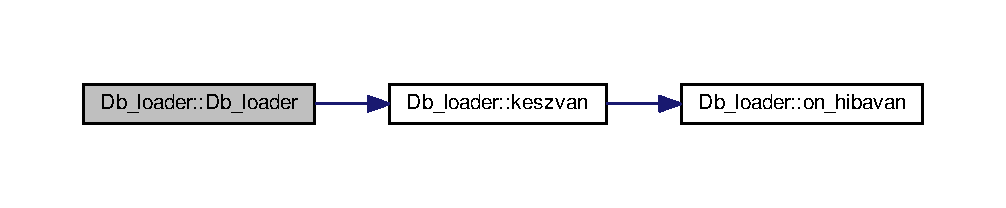
\includegraphics[width=350pt]{classDb__loader_a3a0062be83bea07369d7b6ab0fc77444_cgraph}
\end{center}
\end{figure}
\mbox{\Hypertarget{classDb__loader_a4e14668e7c5243ad9369914343201003}\label{classDb__loader_a4e14668e7c5243ad9369914343201003}} 
\index{Db\+\_\+loader@{Db\+\_\+loader}!````~Db\+\_\+loader@{$\sim$\+Db\+\_\+loader}}
\index{````~Db\+\_\+loader@{$\sim$\+Db\+\_\+loader}!Db\+\_\+loader@{Db\+\_\+loader}}
\subsubsection{\texorpdfstring{$\sim$\+Db\+\_\+loader()}{~Db\_loader()}}
{\footnotesize\ttfamily Db\+\_\+loader\+::$\sim$\+Db\+\_\+loader (\begin{DoxyParamCaption}{ }\end{DoxyParamCaption})}



Definition at line 41 of file db\+\_\+loader.\+cpp.



\subsection{Member Function Documentation}
\mbox{\Hypertarget{classDb__loader_ac2b4287582e909c978a7ef903080a791}\label{classDb__loader_ac2b4287582e909c978a7ef903080a791}} 
\index{Db\+\_\+loader@{Db\+\_\+loader}!elfogadva@{elfogadva}}
\index{elfogadva@{elfogadva}!Db\+\_\+loader@{Db\+\_\+loader}}
\subsubsection{\texorpdfstring{elfogadva}{elfogadva}}
{\footnotesize\ttfamily void Db\+\_\+loader\+::elfogadva (\begin{DoxyParamCaption}\item[{Q\+Standard\+Item\+Model $\ast$}]{exercise }\end{DoxyParamCaption})\hspace{0.3cm}{\ttfamily [signal]}}

Here is the caller graph for this function\+:\nopagebreak
\begin{figure}[H]
\begin{center}
\leavevmode
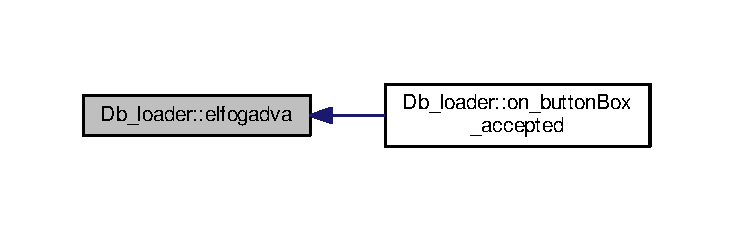
\includegraphics[width=350pt]{classDb__loader_ac2b4287582e909c978a7ef903080a791_icgraph}
\end{center}
\end{figure}
\mbox{\Hypertarget{classDb__loader_a3d308bb09c20a83faa4da10aae8bca27}\label{classDb__loader_a3d308bb09c20a83faa4da10aae8bca27}} 
\index{Db\+\_\+loader@{Db\+\_\+loader}!keszvan@{keszvan}}
\index{keszvan@{keszvan}!Db\+\_\+loader@{Db\+\_\+loader}}
\subsubsection{\texorpdfstring{keszvan}{keszvan}}
{\footnotesize\ttfamily void Db\+\_\+loader\+::keszvan (\begin{DoxyParamCaption}{ }\end{DoxyParamCaption})\hspace{0.3cm}{\ttfamily [private]}, {\ttfamily [slot]}}



Definition at line 58 of file db\+\_\+loader.\+cpp.

Here is the call graph for this function\+:\nopagebreak
\begin{figure}[H]
\begin{center}
\leavevmode
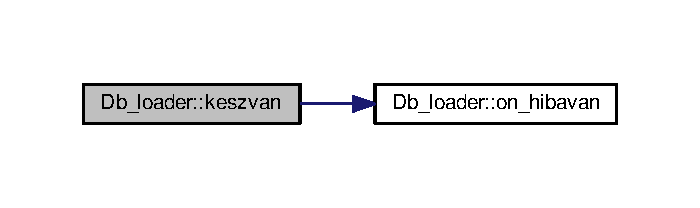
\includegraphics[width=336pt]{classDb__loader_a3d308bb09c20a83faa4da10aae8bca27_cgraph}
\end{center}
\end{figure}
Here is the caller graph for this function\+:\nopagebreak
\begin{figure}[H]
\begin{center}
\leavevmode
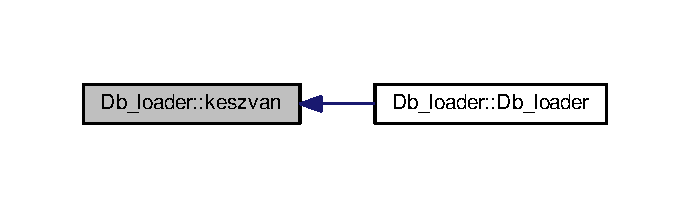
\includegraphics[width=331pt]{classDb__loader_a3d308bb09c20a83faa4da10aae8bca27_icgraph}
\end{center}
\end{figure}
\mbox{\Hypertarget{classDb__loader_a089a424b1719bfbf4068b10bd1070614}\label{classDb__loader_a089a424b1719bfbf4068b10bd1070614}} 
\index{Db\+\_\+loader@{Db\+\_\+loader}!keszvan\+\_\+elem@{keszvan\+\_\+elem}}
\index{keszvan\+\_\+elem@{keszvan\+\_\+elem}!Db\+\_\+loader@{Db\+\_\+loader}}
\subsubsection{\texorpdfstring{keszvan\+\_\+elem}{keszvan\_elem}}
{\footnotesize\ttfamily void Db\+\_\+loader\+::keszvan\+\_\+elem (\begin{DoxyParamCaption}{ }\end{DoxyParamCaption})\hspace{0.3cm}{\ttfamily [private]}, {\ttfamily [slot]}}



Definition at line 100 of file db\+\_\+loader.\+cpp.

Here is the call graph for this function\+:\nopagebreak
\begin{figure}[H]
\begin{center}
\leavevmode
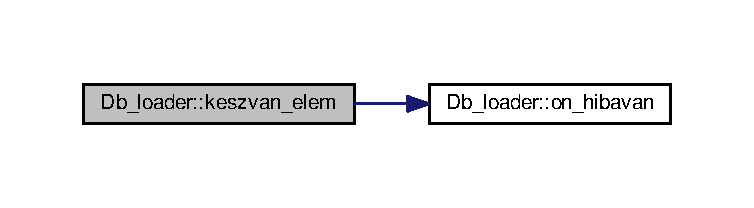
\includegraphics[width=350pt]{classDb__loader_a089a424b1719bfbf4068b10bd1070614_cgraph}
\end{center}
\end{figure}
Here is the caller graph for this function\+:\nopagebreak
\begin{figure}[H]
\begin{center}
\leavevmode
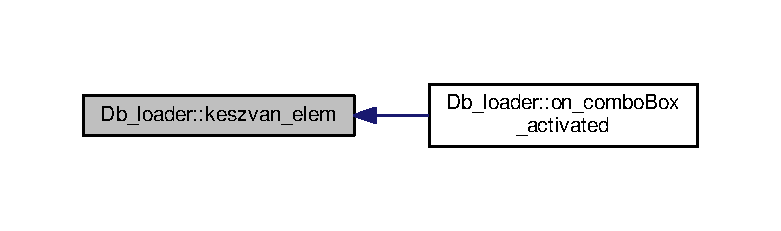
\includegraphics[width=350pt]{classDb__loader_a089a424b1719bfbf4068b10bd1070614_icgraph}
\end{center}
\end{figure}
\mbox{\Hypertarget{classDb__loader_a29a8fa0c0dbc868c7ef0836b27d078f3}\label{classDb__loader_a29a8fa0c0dbc868c7ef0836b27d078f3}} 
\index{Db\+\_\+loader@{Db\+\_\+loader}!on\+\_\+button\+Box\+\_\+accepted@{on\+\_\+button\+Box\+\_\+accepted}}
\index{on\+\_\+button\+Box\+\_\+accepted@{on\+\_\+button\+Box\+\_\+accepted}!Db\+\_\+loader@{Db\+\_\+loader}}
\subsubsection{\texorpdfstring{on\+\_\+button\+Box\+\_\+accepted}{on\_buttonBox\_accepted}}
{\footnotesize\ttfamily void Db\+\_\+loader\+::on\+\_\+button\+Box\+\_\+accepted (\begin{DoxyParamCaption}{ }\end{DoxyParamCaption})\hspace{0.3cm}{\ttfamily [private]}, {\ttfamily [slot]}}



Definition at line 141 of file db\+\_\+loader.\+cpp.

\mbox{\Hypertarget{classDb__loader_af4abb62f67a8c249ddd84a78966acd8b}\label{classDb__loader_af4abb62f67a8c249ddd84a78966acd8b}} 
\index{Db\+\_\+loader@{Db\+\_\+loader}!on\+\_\+combo\+Box\+\_\+activated@{on\+\_\+combo\+Box\+\_\+activated}}
\index{on\+\_\+combo\+Box\+\_\+activated@{on\+\_\+combo\+Box\+\_\+activated}!Db\+\_\+loader@{Db\+\_\+loader}}
\subsubsection{\texorpdfstring{on\+\_\+combo\+Box\+\_\+activated}{on\_comboBox\_activated}}
{\footnotesize\ttfamily void Db\+\_\+loader\+::on\+\_\+combo\+Box\+\_\+activated (\begin{DoxyParamCaption}\item[{const Q\+String \&}]{arg1 }\end{DoxyParamCaption})\hspace{0.3cm}{\ttfamily [private]}, {\ttfamily [slot]}}



Definition at line 46 of file db\+\_\+loader.\+cpp.

Here is the call graph for this function\+:\nopagebreak
\begin{figure}[H]
\begin{center}
\leavevmode
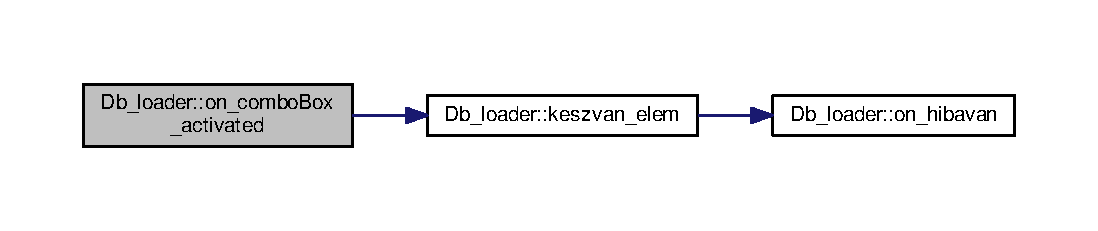
\includegraphics[width=350pt]{classDb__loader_af4abb62f67a8c249ddd84a78966acd8b_cgraph}
\end{center}
\end{figure}
\mbox{\Hypertarget{classDb__loader_aebf68b20ad5c3c7bac822b7c41f4e4ff}\label{classDb__loader_aebf68b20ad5c3c7bac822b7c41f4e4ff}} 
\index{Db\+\_\+loader@{Db\+\_\+loader}!on\+\_\+hibavan@{on\+\_\+hibavan}}
\index{on\+\_\+hibavan@{on\+\_\+hibavan}!Db\+\_\+loader@{Db\+\_\+loader}}
\subsubsection{\texorpdfstring{on\+\_\+hibavan()}{on\_hibavan()}}
{\footnotesize\ttfamily void Db\+\_\+loader\+::on\+\_\+hibavan (\begin{DoxyParamCaption}{ }\end{DoxyParamCaption})\hspace{0.3cm}{\ttfamily [private]}}



Definition at line 93 of file db\+\_\+loader.\+cpp.

Here is the caller graph for this function\+:\nopagebreak
\begin{figure}[H]
\begin{center}
\leavevmode
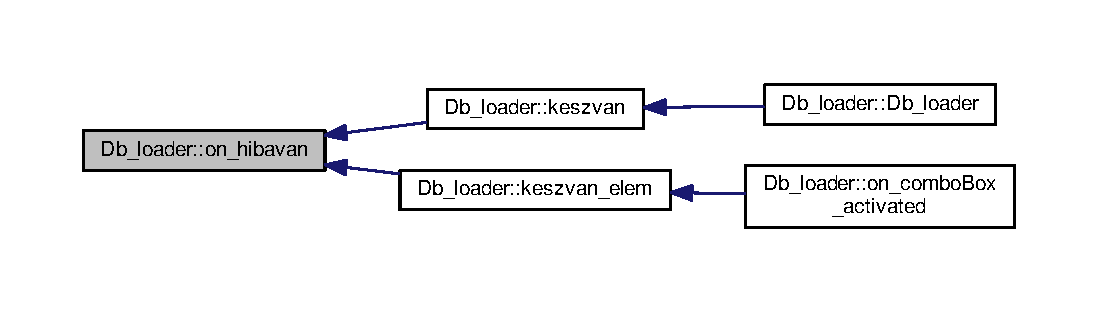
\includegraphics[width=350pt]{classDb__loader_aebf68b20ad5c3c7bac822b7c41f4e4ff_icgraph}
\end{center}
\end{figure}


\subsection{Member Data Documentation}
\mbox{\Hypertarget{classDb__loader_a2f830277361852656d3883ed25a9637d}\label{classDb__loader_a2f830277361852656d3883ed25a9637d}} 
\index{Db\+\_\+loader@{Db\+\_\+loader}!baseurl@{baseurl}}
\index{baseurl@{baseurl}!Db\+\_\+loader@{Db\+\_\+loader}}
\subsubsection{\texorpdfstring{baseurl}{baseurl}}
{\footnotesize\ttfamily Q\+String Db\+\_\+loader\+::baseurl\hspace{0.3cm}{\ttfamily [private]}}



Definition at line 37 of file db\+\_\+loader.\+h.

\mbox{\Hypertarget{classDb__loader_ae2bf960f9be242be7b72496bd28fb2b3}\label{classDb__loader_ae2bf960f9be242be7b72496bd28fb2b3}} 
\index{Db\+\_\+loader@{Db\+\_\+loader}!exercise@{exercise}}
\index{exercise@{exercise}!Db\+\_\+loader@{Db\+\_\+loader}}
\subsubsection{\texorpdfstring{exercise}{exercise}}
{\footnotesize\ttfamily Q\+Standard\+Item\+Model$\ast$ Db\+\_\+loader\+::exercise\hspace{0.3cm}{\ttfamily [private]}}



Definition at line 35 of file db\+\_\+loader.\+h.

\mbox{\Hypertarget{classDb__loader_af15e4654bb9e65eefdbcdfa9ac4fe816}\label{classDb__loader_af15e4654bb9e65eefdbcdfa9ac4fe816}} 
\index{Db\+\_\+loader@{Db\+\_\+loader}!network\+\_\+manager@{network\+\_\+manager}}
\index{network\+\_\+manager@{network\+\_\+manager}!Db\+\_\+loader@{Db\+\_\+loader}}
\subsubsection{\texorpdfstring{network\+\_\+manager}{network\_manager}}
{\footnotesize\ttfamily Q\+Network\+Access\+Manager$\ast$ Db\+\_\+loader\+::network\+\_\+manager\hspace{0.3cm}{\ttfamily [private]}}



Definition at line 36 of file db\+\_\+loader.\+h.

\mbox{\Hypertarget{classDb__loader_aa845f4b8ed46a42205b214db633ff141}\label{classDb__loader_aa845f4b8ed46a42205b214db633ff141}} 
\index{Db\+\_\+loader@{Db\+\_\+loader}!reply@{reply}}
\index{reply@{reply}!Db\+\_\+loader@{Db\+\_\+loader}}
\subsubsection{\texorpdfstring{reply}{reply}}
{\footnotesize\ttfamily Q\+Network\+Reply$\ast$ Db\+\_\+loader\+::reply\hspace{0.3cm}{\ttfamily [private]}}



Definition at line 39 of file db\+\_\+loader.\+h.

\mbox{\Hypertarget{classDb__loader_abe12d8b3b8b23aeb4c70dc8cb103b33e}\label{classDb__loader_abe12d8b3b8b23aeb4c70dc8cb103b33e}} 
\index{Db\+\_\+loader@{Db\+\_\+loader}!reply2@{reply2}}
\index{reply2@{reply2}!Db\+\_\+loader@{Db\+\_\+loader}}
\subsubsection{\texorpdfstring{reply2}{reply2}}
{\footnotesize\ttfamily Q\+Network\+Reply$\ast$ Db\+\_\+loader\+::reply2 \{\}\hspace{0.3cm}{\ttfamily [private]}}



Definition at line 40 of file db\+\_\+loader.\+h.

\mbox{\Hypertarget{classDb__loader_a3bf15a8ed1216c614b030610cebabaeb}\label{classDb__loader_a3bf15a8ed1216c614b030610cebabaeb}} 
\index{Db\+\_\+loader@{Db\+\_\+loader}!req@{req}}
\index{req@{req}!Db\+\_\+loader@{Db\+\_\+loader}}
\subsubsection{\texorpdfstring{req}{req}}
{\footnotesize\ttfamily Q\+Network\+Request Db\+\_\+loader\+::req\hspace{0.3cm}{\ttfamily [private]}}



Definition at line 38 of file db\+\_\+loader.\+h.

\mbox{\Hypertarget{classDb__loader_a7bc8f5be142eb2ad90de8682268224ae}\label{classDb__loader_a7bc8f5be142eb2ad90de8682268224ae}} 
\index{Db\+\_\+loader@{Db\+\_\+loader}!ui@{ui}}
\index{ui@{ui}!Db\+\_\+loader@{Db\+\_\+loader}}
\subsubsection{\texorpdfstring{ui}{ui}}
{\footnotesize\ttfamily Ui\+::\+Db\+\_\+loader$\ast$ Db\+\_\+loader\+::ui\hspace{0.3cm}{\ttfamily [private]}}



Definition at line 34 of file db\+\_\+loader.\+h.



The documentation for this class was generated from the following files\+:\begin{DoxyCompactItemize}
\item 
Exercise\+\_\+\+Load\+\_\+\+Plugin/\hyperlink{db__loader_8h}{db\+\_\+loader.\+h}\item 
Exercise\+\_\+\+Load\+\_\+\+Plugin/\hyperlink{db__loader_8cpp}{db\+\_\+loader.\+cpp}\end{DoxyCompactItemize}

\hypertarget{classDelegate__for__numbers}{}\section{Delegate\+\_\+for\+\_\+numbers Class Reference}
\label{classDelegate__for__numbers}\index{Delegate\+\_\+for\+\_\+numbers@{Delegate\+\_\+for\+\_\+numbers}}


{\ttfamily \#include $<$delegate\+\_\+for\+\_\+numbers.\+h$>$}



Inherits Q\+Styled\+Item\+Delegate.

\subsection*{Public Member Functions}
\begin{DoxyCompactItemize}
\item 
\hyperlink{classDelegate__for__numbers_a16e922f8dcb025c5587eb072b189ec9d}{Delegate\+\_\+for\+\_\+numbers} (Q\+Object $\ast$parent=nullptr)
\item 
Q\+Widget $\ast$ \hyperlink{classDelegate__for__numbers_a4b9f325ef5ff87188af3228bf8d29372}{create\+Editor} (Q\+Widget $\ast$parent, const Q\+Style\+Option\+View\+Item \&option, const Q\+Model\+Index \&index) const Q\+\_\+\+D\+E\+C\+L\+\_\+\+O\+V\+E\+R\+R\+I\+DE
\item 
void \hyperlink{classDelegate__for__numbers_a182eaf8c7d3306a22415315fe53577d3}{set\+Editor\+Data} (Q\+Widget $\ast$editor, const Q\+Model\+Index \&index) const Q\+\_\+\+D\+E\+C\+L\+\_\+\+O\+V\+E\+R\+R\+I\+DE
\begin{DoxyCompactList}\small\item\em \mbox{[}1\mbox{]} \end{DoxyCompactList}\item 
void \hyperlink{classDelegate__for__numbers_a99f27c00eea2aa04248cb3410a9557de}{set\+Model\+Data} (Q\+Widget $\ast$editor, Q\+Abstract\+Item\+Model $\ast$model, const Q\+Model\+Index \&index) const Q\+\_\+\+D\+E\+C\+L\+\_\+\+O\+V\+E\+R\+R\+I\+DE
\begin{DoxyCompactList}\small\item\em \mbox{[}2\mbox{]} \end{DoxyCompactList}\item 
void \hyperlink{classDelegate__for__numbers_aa8c3d2a65f804ee47df6b938f834c9ca}{update\+Editor\+Geometry} (Q\+Widget $\ast$editor, const Q\+Style\+Option\+View\+Item \&option, const Q\+Model\+Index \&index) const Q\+\_\+\+D\+E\+C\+L\+\_\+\+O\+V\+E\+R\+R\+I\+DE
\begin{DoxyCompactList}\small\item\em \mbox{[}3\mbox{]} \end{DoxyCompactList}\end{DoxyCompactItemize}


\subsection{Detailed Description}


Definition at line 5 of file delegate\+\_\+for\+\_\+numbers.\+h.



\subsection{Constructor \& Destructor Documentation}
\mbox{\Hypertarget{classDelegate__for__numbers_a16e922f8dcb025c5587eb072b189ec9d}\label{classDelegate__for__numbers_a16e922f8dcb025c5587eb072b189ec9d}} 
\index{Delegate\+\_\+for\+\_\+numbers@{Delegate\+\_\+for\+\_\+numbers}!Delegate\+\_\+for\+\_\+numbers@{Delegate\+\_\+for\+\_\+numbers}}
\index{Delegate\+\_\+for\+\_\+numbers@{Delegate\+\_\+for\+\_\+numbers}!Delegate\+\_\+for\+\_\+numbers@{Delegate\+\_\+for\+\_\+numbers}}
\subsubsection{\texorpdfstring{Delegate\+\_\+for\+\_\+numbers()}{Delegate\_for\_numbers()}}
{\footnotesize\ttfamily Delegate\+\_\+for\+\_\+numbers\+::\+Delegate\+\_\+for\+\_\+numbers (\begin{DoxyParamCaption}\item[{Q\+Object $\ast$}]{parent = {\ttfamily nullptr} }\end{DoxyParamCaption})}



Definition at line 4 of file delegate\+\_\+for\+\_\+numbers.\+cpp.



\subsection{Member Function Documentation}
\mbox{\Hypertarget{classDelegate__for__numbers_a4b9f325ef5ff87188af3228bf8d29372}\label{classDelegate__for__numbers_a4b9f325ef5ff87188af3228bf8d29372}} 
\index{Delegate\+\_\+for\+\_\+numbers@{Delegate\+\_\+for\+\_\+numbers}!create\+Editor@{create\+Editor}}
\index{create\+Editor@{create\+Editor}!Delegate\+\_\+for\+\_\+numbers@{Delegate\+\_\+for\+\_\+numbers}}
\subsubsection{\texorpdfstring{create\+Editor()}{createEditor()}}
{\footnotesize\ttfamily Q\+Widget $\ast$ Delegate\+\_\+for\+\_\+numbers\+::create\+Editor (\begin{DoxyParamCaption}\item[{Q\+Widget $\ast$}]{parent,  }\item[{const Q\+Style\+Option\+View\+Item \&}]{option,  }\item[{const Q\+Model\+Index \&}]{index }\end{DoxyParamCaption}) const}



Definition at line 8 of file delegate\+\_\+for\+\_\+numbers.\+cpp.

\mbox{\Hypertarget{classDelegate__for__numbers_a182eaf8c7d3306a22415315fe53577d3}\label{classDelegate__for__numbers_a182eaf8c7d3306a22415315fe53577d3}} 
\index{Delegate\+\_\+for\+\_\+numbers@{Delegate\+\_\+for\+\_\+numbers}!set\+Editor\+Data@{set\+Editor\+Data}}
\index{set\+Editor\+Data@{set\+Editor\+Data}!Delegate\+\_\+for\+\_\+numbers@{Delegate\+\_\+for\+\_\+numbers}}
\subsubsection{\texorpdfstring{set\+Editor\+Data()}{setEditorData()}}
{\footnotesize\ttfamily void Delegate\+\_\+for\+\_\+numbers\+::set\+Editor\+Data (\begin{DoxyParamCaption}\item[{Q\+Widget $\ast$}]{editor,  }\item[{const Q\+Model\+Index \&}]{index }\end{DoxyParamCaption}) const}



\mbox{[}1\mbox{]} 

\mbox{[}2\mbox{]} 

Definition at line 24 of file delegate\+\_\+for\+\_\+numbers.\+cpp.

\mbox{\Hypertarget{classDelegate__for__numbers_a99f27c00eea2aa04248cb3410a9557de}\label{classDelegate__for__numbers_a99f27c00eea2aa04248cb3410a9557de}} 
\index{Delegate\+\_\+for\+\_\+numbers@{Delegate\+\_\+for\+\_\+numbers}!set\+Model\+Data@{set\+Model\+Data}}
\index{set\+Model\+Data@{set\+Model\+Data}!Delegate\+\_\+for\+\_\+numbers@{Delegate\+\_\+for\+\_\+numbers}}
\subsubsection{\texorpdfstring{set\+Model\+Data()}{setModelData()}}
{\footnotesize\ttfamily void Delegate\+\_\+for\+\_\+numbers\+::set\+Model\+Data (\begin{DoxyParamCaption}\item[{Q\+Widget $\ast$}]{editor,  }\item[{Q\+Abstract\+Item\+Model $\ast$}]{model,  }\item[{const Q\+Model\+Index \&}]{index }\end{DoxyParamCaption}) const}



\mbox{[}2\mbox{]} 

\mbox{[}3\mbox{]} 

Definition at line 35 of file delegate\+\_\+for\+\_\+numbers.\+cpp.

\mbox{\Hypertarget{classDelegate__for__numbers_aa8c3d2a65f804ee47df6b938f834c9ca}\label{classDelegate__for__numbers_aa8c3d2a65f804ee47df6b938f834c9ca}} 
\index{Delegate\+\_\+for\+\_\+numbers@{Delegate\+\_\+for\+\_\+numbers}!update\+Editor\+Geometry@{update\+Editor\+Geometry}}
\index{update\+Editor\+Geometry@{update\+Editor\+Geometry}!Delegate\+\_\+for\+\_\+numbers@{Delegate\+\_\+for\+\_\+numbers}}
\subsubsection{\texorpdfstring{update\+Editor\+Geometry()}{updateEditorGeometry()}}
{\footnotesize\ttfamily void Delegate\+\_\+for\+\_\+numbers\+::update\+Editor\+Geometry (\begin{DoxyParamCaption}\item[{Q\+Widget $\ast$}]{editor,  }\item[{const Q\+Style\+Option\+View\+Item \&}]{option,  }\item[{const Q\+Model\+Index \&}]{index }\end{DoxyParamCaption}) const}



\mbox{[}3\mbox{]} 

\mbox{[}4\mbox{]} 

Definition at line 47 of file delegate\+\_\+for\+\_\+numbers.\+cpp.



The documentation for this class was generated from the following files\+:\begin{DoxyCompactItemize}
\item 
simplex\+\_\+app/\hyperlink{delegate__for__numbers_8h}{delegate\+\_\+for\+\_\+numbers.\+h}\item 
simplex\+\_\+app/\hyperlink{delegate__for__numbers_8cpp}{delegate\+\_\+for\+\_\+numbers.\+cpp}\end{DoxyCompactItemize}

\hypertarget{classDelegate__for__numbers__in__fules}{}\section{Delegate\+\_\+for\+\_\+numbers\+\_\+in\+\_\+fules Class Reference}
\label{classDelegate__for__numbers__in__fules}\index{Delegate\+\_\+for\+\_\+numbers\+\_\+in\+\_\+fules@{Delegate\+\_\+for\+\_\+numbers\+\_\+in\+\_\+fules}}


{\ttfamily \#include $<$delegate\+\_\+for\+\_\+numbers\+\_\+in\+\_\+fules.\+h$>$}



Inherits Q\+Styled\+Item\+Delegate.

\subsection*{Public Member Functions}
\begin{DoxyCompactItemize}
\item 
\hyperlink{classDelegate__for__numbers__in__fules_a063ab9cc8f84dc63285f863f6b447562}{Delegate\+\_\+for\+\_\+numbers\+\_\+in\+\_\+fules} (Q\+Object $\ast$parent=nullptr)
\item 
Q\+Widget $\ast$ \hyperlink{classDelegate__for__numbers__in__fules_a08e0cd3a839dbef91678350bf25dd163}{create\+Editor} (Q\+Widget $\ast$parent, const Q\+Style\+Option\+View\+Item \&option, const Q\+Model\+Index \&index) const Q\+\_\+\+D\+E\+C\+L\+\_\+\+O\+V\+E\+R\+R\+I\+DE
\item 
void \hyperlink{classDelegate__for__numbers__in__fules_a8ed7d13b0ce16e8c830de737d5354725}{set\+Editor\+Data} (Q\+Widget $\ast$editor, const Q\+Model\+Index \&index) const Q\+\_\+\+D\+E\+C\+L\+\_\+\+O\+V\+E\+R\+R\+I\+DE
\begin{DoxyCompactList}\small\item\em \mbox{[}1\mbox{]} \end{DoxyCompactList}\item 
void \hyperlink{classDelegate__for__numbers__in__fules_a0f0422051323d15ae95017008aa1bac1}{set\+Model\+Data} (Q\+Widget $\ast$editor, Q\+Abstract\+Item\+Model $\ast$model, const Q\+Model\+Index \&index) const Q\+\_\+\+D\+E\+C\+L\+\_\+\+O\+V\+E\+R\+R\+I\+DE
\begin{DoxyCompactList}\small\item\em \mbox{[}2\mbox{]} \end{DoxyCompactList}\item 
void \hyperlink{classDelegate__for__numbers__in__fules_a2c2d5f81ed07f0992f692e6858d13aaf}{update\+Editor\+Geometry} (Q\+Widget $\ast$editor, const Q\+Style\+Option\+View\+Item \&option, const Q\+Model\+Index \&index) const Q\+\_\+\+D\+E\+C\+L\+\_\+\+O\+V\+E\+R\+R\+I\+DE
\begin{DoxyCompactList}\small\item\em \mbox{[}3\mbox{]} \end{DoxyCompactList}\end{DoxyCompactItemize}


\subsection{Detailed Description}


Definition at line 5 of file delegate\+\_\+for\+\_\+numbers\+\_\+in\+\_\+fules.\+h.



\subsection{Constructor \& Destructor Documentation}
\mbox{\Hypertarget{classDelegate__for__numbers__in__fules_a063ab9cc8f84dc63285f863f6b447562}\label{classDelegate__for__numbers__in__fules_a063ab9cc8f84dc63285f863f6b447562}} 
\index{Delegate\+\_\+for\+\_\+numbers\+\_\+in\+\_\+fules@{Delegate\+\_\+for\+\_\+numbers\+\_\+in\+\_\+fules}!Delegate\+\_\+for\+\_\+numbers\+\_\+in\+\_\+fules@{Delegate\+\_\+for\+\_\+numbers\+\_\+in\+\_\+fules}}
\index{Delegate\+\_\+for\+\_\+numbers\+\_\+in\+\_\+fules@{Delegate\+\_\+for\+\_\+numbers\+\_\+in\+\_\+fules}!Delegate\+\_\+for\+\_\+numbers\+\_\+in\+\_\+fules@{Delegate\+\_\+for\+\_\+numbers\+\_\+in\+\_\+fules}}
\subsubsection{\texorpdfstring{Delegate\+\_\+for\+\_\+numbers\+\_\+in\+\_\+fules()}{Delegate\_for\_numbers\_in\_fules()}}
{\footnotesize\ttfamily Delegate\+\_\+for\+\_\+numbers\+\_\+in\+\_\+fules\+::\+Delegate\+\_\+for\+\_\+numbers\+\_\+in\+\_\+fules (\begin{DoxyParamCaption}\item[{Q\+Object $\ast$}]{parent = {\ttfamily nullptr} }\end{DoxyParamCaption})}



Definition at line 4 of file delegate\+\_\+for\+\_\+numbers\+\_\+in\+\_\+fules.\+cpp.



\subsection{Member Function Documentation}
\mbox{\Hypertarget{classDelegate__for__numbers__in__fules_a08e0cd3a839dbef91678350bf25dd163}\label{classDelegate__for__numbers__in__fules_a08e0cd3a839dbef91678350bf25dd163}} 
\index{Delegate\+\_\+for\+\_\+numbers\+\_\+in\+\_\+fules@{Delegate\+\_\+for\+\_\+numbers\+\_\+in\+\_\+fules}!create\+Editor@{create\+Editor}}
\index{create\+Editor@{create\+Editor}!Delegate\+\_\+for\+\_\+numbers\+\_\+in\+\_\+fules@{Delegate\+\_\+for\+\_\+numbers\+\_\+in\+\_\+fules}}
\subsubsection{\texorpdfstring{create\+Editor()}{createEditor()}}
{\footnotesize\ttfamily Q\+Widget $\ast$ Delegate\+\_\+for\+\_\+numbers\+\_\+in\+\_\+fules\+::create\+Editor (\begin{DoxyParamCaption}\item[{Q\+Widget $\ast$}]{parent,  }\item[{const Q\+Style\+Option\+View\+Item \&}]{option,  }\item[{const Q\+Model\+Index \&}]{index }\end{DoxyParamCaption}) const}



Definition at line 8 of file delegate\+\_\+for\+\_\+numbers\+\_\+in\+\_\+fules.\+cpp.

\mbox{\Hypertarget{classDelegate__for__numbers__in__fules_a8ed7d13b0ce16e8c830de737d5354725}\label{classDelegate__for__numbers__in__fules_a8ed7d13b0ce16e8c830de737d5354725}} 
\index{Delegate\+\_\+for\+\_\+numbers\+\_\+in\+\_\+fules@{Delegate\+\_\+for\+\_\+numbers\+\_\+in\+\_\+fules}!set\+Editor\+Data@{set\+Editor\+Data}}
\index{set\+Editor\+Data@{set\+Editor\+Data}!Delegate\+\_\+for\+\_\+numbers\+\_\+in\+\_\+fules@{Delegate\+\_\+for\+\_\+numbers\+\_\+in\+\_\+fules}}
\subsubsection{\texorpdfstring{set\+Editor\+Data()}{setEditorData()}}
{\footnotesize\ttfamily void Delegate\+\_\+for\+\_\+numbers\+\_\+in\+\_\+fules\+::set\+Editor\+Data (\begin{DoxyParamCaption}\item[{Q\+Widget $\ast$}]{editor,  }\item[{const Q\+Model\+Index \&}]{index }\end{DoxyParamCaption}) const}



\mbox{[}1\mbox{]} 

\mbox{[}2\mbox{]} 

Definition at line 24 of file delegate\+\_\+for\+\_\+numbers\+\_\+in\+\_\+fules.\+cpp.

\mbox{\Hypertarget{classDelegate__for__numbers__in__fules_a0f0422051323d15ae95017008aa1bac1}\label{classDelegate__for__numbers__in__fules_a0f0422051323d15ae95017008aa1bac1}} 
\index{Delegate\+\_\+for\+\_\+numbers\+\_\+in\+\_\+fules@{Delegate\+\_\+for\+\_\+numbers\+\_\+in\+\_\+fules}!set\+Model\+Data@{set\+Model\+Data}}
\index{set\+Model\+Data@{set\+Model\+Data}!Delegate\+\_\+for\+\_\+numbers\+\_\+in\+\_\+fules@{Delegate\+\_\+for\+\_\+numbers\+\_\+in\+\_\+fules}}
\subsubsection{\texorpdfstring{set\+Model\+Data()}{setModelData()}}
{\footnotesize\ttfamily void Delegate\+\_\+for\+\_\+numbers\+\_\+in\+\_\+fules\+::set\+Model\+Data (\begin{DoxyParamCaption}\item[{Q\+Widget $\ast$}]{editor,  }\item[{Q\+Abstract\+Item\+Model $\ast$}]{model,  }\item[{const Q\+Model\+Index \&}]{index }\end{DoxyParamCaption}) const}



\mbox{[}2\mbox{]} 

\mbox{[}3\mbox{]} 

Definition at line 35 of file delegate\+\_\+for\+\_\+numbers\+\_\+in\+\_\+fules.\+cpp.

\mbox{\Hypertarget{classDelegate__for__numbers__in__fules_a2c2d5f81ed07f0992f692e6858d13aaf}\label{classDelegate__for__numbers__in__fules_a2c2d5f81ed07f0992f692e6858d13aaf}} 
\index{Delegate\+\_\+for\+\_\+numbers\+\_\+in\+\_\+fules@{Delegate\+\_\+for\+\_\+numbers\+\_\+in\+\_\+fules}!update\+Editor\+Geometry@{update\+Editor\+Geometry}}
\index{update\+Editor\+Geometry@{update\+Editor\+Geometry}!Delegate\+\_\+for\+\_\+numbers\+\_\+in\+\_\+fules@{Delegate\+\_\+for\+\_\+numbers\+\_\+in\+\_\+fules}}
\subsubsection{\texorpdfstring{update\+Editor\+Geometry()}{updateEditorGeometry()}}
{\footnotesize\ttfamily void Delegate\+\_\+for\+\_\+numbers\+\_\+in\+\_\+fules\+::update\+Editor\+Geometry (\begin{DoxyParamCaption}\item[{Q\+Widget $\ast$}]{editor,  }\item[{const Q\+Style\+Option\+View\+Item \&}]{option,  }\item[{const Q\+Model\+Index \&}]{index }\end{DoxyParamCaption}) const}



\mbox{[}3\mbox{]} 

\mbox{[}4\mbox{]} 

Definition at line 47 of file delegate\+\_\+for\+\_\+numbers\+\_\+in\+\_\+fules.\+cpp.



The documentation for this class was generated from the following files\+:\begin{DoxyCompactItemize}
\item 
fules/\hyperlink{delegate__for__numbers__in__fules_8h}{delegate\+\_\+for\+\_\+numbers\+\_\+in\+\_\+fules.\+h}\item 
fules/\hyperlink{delegate__for__numbers__in__fules_8cpp}{delegate\+\_\+for\+\_\+numbers\+\_\+in\+\_\+fules.\+cpp}\end{DoxyCompactItemize}

\hypertarget{classExercise__Load__Plugin}{}\section{Exercise\+\_\+\+Load\+\_\+\+Plugin Class Reference}
\label{classExercise__Load__Plugin}\index{Exercise\+\_\+\+Load\+\_\+\+Plugin@{Exercise\+\_\+\+Load\+\_\+\+Plugin}}


{\ttfamily \#include $<$exercise\+\_\+load\+\_\+plugin.\+h$>$}



Inheritance diagram for Exercise\+\_\+\+Load\+\_\+\+Plugin\+:\nopagebreak
\begin{figure}[H]
\begin{center}
\leavevmode
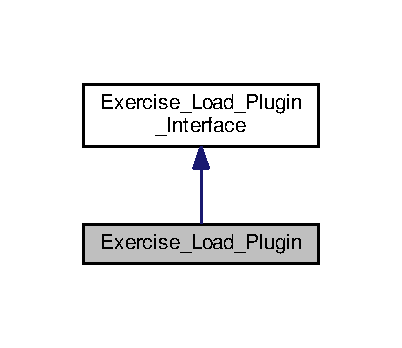
\includegraphics[width=193pt]{classExercise__Load__Plugin__inherit__graph}
\end{center}
\end{figure}


Collaboration diagram for Exercise\+\_\+\+Load\+\_\+\+Plugin\+:\nopagebreak
\begin{figure}[H]
\begin{center}
\leavevmode
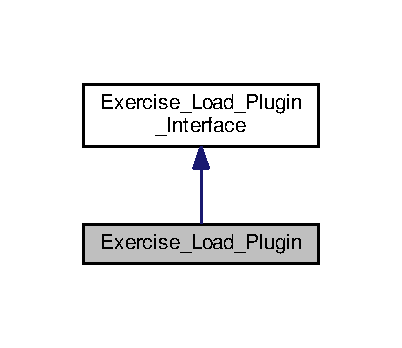
\includegraphics[width=193pt]{classExercise__Load__Plugin__coll__graph}
\end{center}
\end{figure}
\subsection*{Public Slots}
\begin{DoxyCompactItemize}
\item 
void \hyperlink{classExercise__Load__Plugin_af4de0753b05095fed82d7955a0e32cf8}{do\+\_\+elfogadva} (Q\+Standard\+Item\+Model $\ast$\hyperlink{classExercise__Load__Plugin_ab2c84c55120579b1fdb135eb73694837}{exercise})
\end{DoxyCompactItemize}
\subsection*{Signals}
\begin{DoxyCompactItemize}
\item 
void \hyperlink{classExercise__Load__Plugin_a81e0284dc19303bfb0408cf14247ea9c}{do\+\_\+post\+\_\+exercise} (Q\+Standard\+Item\+Model $\ast$) Q\+\_\+\+D\+E\+C\+L\+\_\+\+F\+I\+N\+AL
\end{DoxyCompactItemize}
\subsection*{Public Member Functions}
\begin{DoxyCompactItemize}
\item 
\hyperlink{classExercise__Load__Plugin_a23574d3050cd6fd13c7387b76deb22fd}{Exercise\+\_\+\+Load\+\_\+\+Plugin} (Q\+Widget $\ast$parent=nullptr)
\item 
void \hyperlink{classExercise__Load__Plugin_ad0c7c810dd492a014e17d40cdfe3d35d}{post\+\_\+exercise} (Q\+Standard\+Item\+Model $\ast$\hyperlink{classExercise__Load__Plugin_ab2c84c55120579b1fdb135eb73694837}{exercise}) Q\+\_\+\+D\+E\+C\+L\+\_\+\+O\+V\+E\+R\+R\+I\+DE
\end{DoxyCompactItemize}
\subsection*{Private Member Functions}
\begin{DoxyCompactItemize}
\item 
Q\+String \hyperlink{classExercise__Load__Plugin_af6226d33bef2f1f526a8f37ec33e431c}{Name} () const override
\item 
Q\+Standard\+Item\+Model $\ast$ \hyperlink{classExercise__Load__Plugin_ab2c84c55120579b1fdb135eb73694837}{exercise} ()
\end{DoxyCompactItemize}


\subsection{Detailed Description}


Definition at line 8 of file exercise\+\_\+load\+\_\+plugin.\+h.



\subsection{Constructor \& Destructor Documentation}
\mbox{\Hypertarget{classExercise__Load__Plugin_a23574d3050cd6fd13c7387b76deb22fd}\label{classExercise__Load__Plugin_a23574d3050cd6fd13c7387b76deb22fd}} 
\index{Exercise\+\_\+\+Load\+\_\+\+Plugin@{Exercise\+\_\+\+Load\+\_\+\+Plugin}!Exercise\+\_\+\+Load\+\_\+\+Plugin@{Exercise\+\_\+\+Load\+\_\+\+Plugin}}
\index{Exercise\+\_\+\+Load\+\_\+\+Plugin@{Exercise\+\_\+\+Load\+\_\+\+Plugin}!Exercise\+\_\+\+Load\+\_\+\+Plugin@{Exercise\+\_\+\+Load\+\_\+\+Plugin}}
\subsubsection{\texorpdfstring{Exercise\+\_\+\+Load\+\_\+\+Plugin()}{Exercise\_Load\_Plugin()}}
{\footnotesize\ttfamily Exercise\+\_\+\+Load\+\_\+\+Plugin\+::\+Exercise\+\_\+\+Load\+\_\+\+Plugin (\begin{DoxyParamCaption}\item[{Q\+Widget $\ast$}]{parent = {\ttfamily nullptr} }\end{DoxyParamCaption})\hspace{0.3cm}{\ttfamily [explicit]}}



Definition at line 4 of file exercise\+\_\+load\+\_\+plugin.\+cpp.



\subsection{Member Function Documentation}
\mbox{\Hypertarget{classExercise__Load__Plugin_af4de0753b05095fed82d7955a0e32cf8}\label{classExercise__Load__Plugin_af4de0753b05095fed82d7955a0e32cf8}} 
\index{Exercise\+\_\+\+Load\+\_\+\+Plugin@{Exercise\+\_\+\+Load\+\_\+\+Plugin}!do\+\_\+elfogadva@{do\+\_\+elfogadva}}
\index{do\+\_\+elfogadva@{do\+\_\+elfogadva}!Exercise\+\_\+\+Load\+\_\+\+Plugin@{Exercise\+\_\+\+Load\+\_\+\+Plugin}}
\subsubsection{\texorpdfstring{do\+\_\+elfogadva}{do\_elfogadva}}
{\footnotesize\ttfamily void Exercise\+\_\+\+Load\+\_\+\+Plugin\+::do\+\_\+elfogadva (\begin{DoxyParamCaption}\item[{Q\+Standard\+Item\+Model $\ast$}]{exercise }\end{DoxyParamCaption})\hspace{0.3cm}{\ttfamily [slot]}}



Definition at line 23 of file exercise\+\_\+load\+\_\+plugin.\+cpp.

Here is the caller graph for this function\+:\nopagebreak
\begin{figure}[H]
\begin{center}
\leavevmode
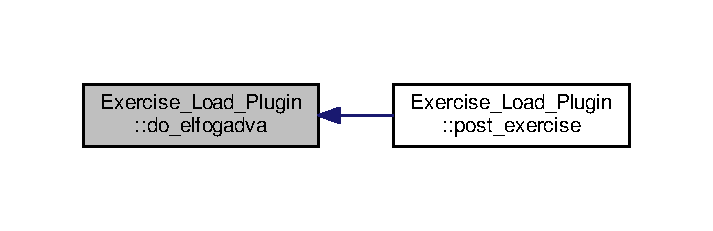
\includegraphics[width=342pt]{classExercise__Load__Plugin_af4de0753b05095fed82d7955a0e32cf8_icgraph}
\end{center}
\end{figure}
\mbox{\Hypertarget{classExercise__Load__Plugin_a81e0284dc19303bfb0408cf14247ea9c}\label{classExercise__Load__Plugin_a81e0284dc19303bfb0408cf14247ea9c}} 
\index{Exercise\+\_\+\+Load\+\_\+\+Plugin@{Exercise\+\_\+\+Load\+\_\+\+Plugin}!do\+\_\+post\+\_\+exercise@{do\+\_\+post\+\_\+exercise}}
\index{do\+\_\+post\+\_\+exercise@{do\+\_\+post\+\_\+exercise}!Exercise\+\_\+\+Load\+\_\+\+Plugin@{Exercise\+\_\+\+Load\+\_\+\+Plugin}}
\subsubsection{\texorpdfstring{do\+\_\+post\+\_\+exercise}{do\_post\_exercise}}
{\footnotesize\ttfamily void Exercise\+\_\+\+Load\+\_\+\+Plugin\+::do\+\_\+post\+\_\+exercise (\begin{DoxyParamCaption}\item[{Q\+Standard\+Item\+Model $\ast$}]{ }\end{DoxyParamCaption})\hspace{0.3cm}{\ttfamily [signal]}}

Here is the caller graph for this function\+:\nopagebreak
\begin{figure}[H]
\begin{center}
\leavevmode
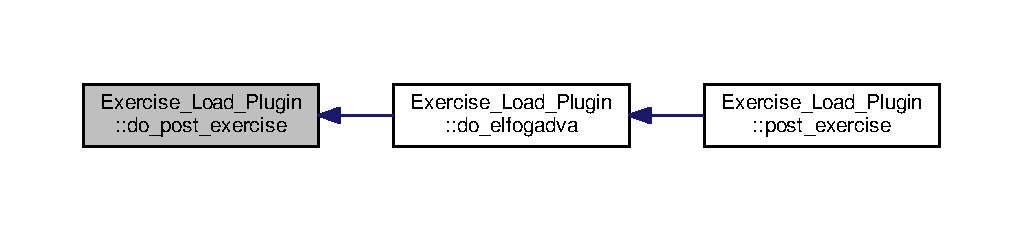
\includegraphics[width=350pt]{classExercise__Load__Plugin_a81e0284dc19303bfb0408cf14247ea9c_icgraph}
\end{center}
\end{figure}
\mbox{\Hypertarget{classExercise__Load__Plugin_ab2c84c55120579b1fdb135eb73694837}\label{classExercise__Load__Plugin_ab2c84c55120579b1fdb135eb73694837}} 
\index{Exercise\+\_\+\+Load\+\_\+\+Plugin@{Exercise\+\_\+\+Load\+\_\+\+Plugin}!exercise@{exercise}}
\index{exercise@{exercise}!Exercise\+\_\+\+Load\+\_\+\+Plugin@{Exercise\+\_\+\+Load\+\_\+\+Plugin}}
\subsubsection{\texorpdfstring{exercise()}{exercise()}}
{\footnotesize\ttfamily Q\+Standard\+Item\+Model$\ast$ Exercise\+\_\+\+Load\+\_\+\+Plugin\+::exercise (\begin{DoxyParamCaption}{ }\end{DoxyParamCaption})\hspace{0.3cm}{\ttfamily [private]}}

\mbox{\Hypertarget{classExercise__Load__Plugin_af6226d33bef2f1f526a8f37ec33e431c}\label{classExercise__Load__Plugin_af6226d33bef2f1f526a8f37ec33e431c}} 
\index{Exercise\+\_\+\+Load\+\_\+\+Plugin@{Exercise\+\_\+\+Load\+\_\+\+Plugin}!Name@{Name}}
\index{Name@{Name}!Exercise\+\_\+\+Load\+\_\+\+Plugin@{Exercise\+\_\+\+Load\+\_\+\+Plugin}}
\subsubsection{\texorpdfstring{Name()}{Name()}}
{\footnotesize\ttfamily Q\+String Exercise\+\_\+\+Load\+\_\+\+Plugin\+::\+Name (\begin{DoxyParamCaption}{ }\end{DoxyParamCaption}) const\hspace{0.3cm}{\ttfamily [override]}, {\ttfamily [private]}, {\ttfamily [virtual]}}



Implements \hyperlink{classExercise__Load__Plugin__Interface_ab6899b947c3890e73b8a64b3c76c60de}{Exercise\+\_\+\+Load\+\_\+\+Plugin\+\_\+\+Interface}.



Definition at line 9 of file exercise\+\_\+load\+\_\+plugin.\+cpp.

\mbox{\Hypertarget{classExercise__Load__Plugin_ad0c7c810dd492a014e17d40cdfe3d35d}\label{classExercise__Load__Plugin_ad0c7c810dd492a014e17d40cdfe3d35d}} 
\index{Exercise\+\_\+\+Load\+\_\+\+Plugin@{Exercise\+\_\+\+Load\+\_\+\+Plugin}!post\+\_\+exercise@{post\+\_\+exercise}}
\index{post\+\_\+exercise@{post\+\_\+exercise}!Exercise\+\_\+\+Load\+\_\+\+Plugin@{Exercise\+\_\+\+Load\+\_\+\+Plugin}}
\subsubsection{\texorpdfstring{post\+\_\+exercise()}{post\_exercise()}}
{\footnotesize\ttfamily void Exercise\+\_\+\+Load\+\_\+\+Plugin\+::post\+\_\+exercise (\begin{DoxyParamCaption}\item[{Q\+Standard\+Item\+Model $\ast$}]{exercise }\end{DoxyParamCaption})\hspace{0.3cm}{\ttfamily [virtual]}}



Implements \hyperlink{classExercise__Load__Plugin__Interface_abb9fef00080e48c6ce458b7476db97d9}{Exercise\+\_\+\+Load\+\_\+\+Plugin\+\_\+\+Interface}.



Definition at line 14 of file exercise\+\_\+load\+\_\+plugin.\+cpp.

Here is the call graph for this function\+:\nopagebreak
\begin{figure}[H]
\begin{center}
\leavevmode
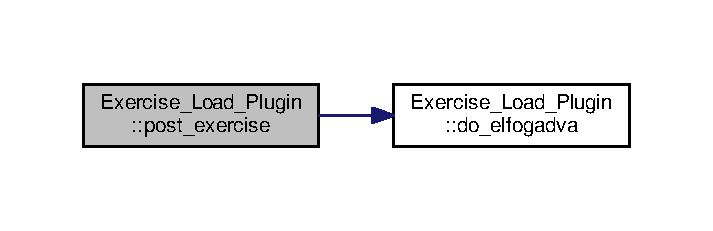
\includegraphics[width=342pt]{classExercise__Load__Plugin_ad0c7c810dd492a014e17d40cdfe3d35d_cgraph}
\end{center}
\end{figure}


The documentation for this class was generated from the following files\+:\begin{DoxyCompactItemize}
\item 
Exercise\+\_\+\+Load\+\_\+\+Plugin/\hyperlink{exercise__load__plugin_8h}{exercise\+\_\+load\+\_\+plugin.\+h}\item 
Exercise\+\_\+\+Load\+\_\+\+Plugin/\hyperlink{exercise__load__plugin_8cpp}{exercise\+\_\+load\+\_\+plugin.\+cpp}\end{DoxyCompactItemize}

\hypertarget{classExercise__Load__Plugin__Interface}{}\section{Exercise\+\_\+\+Load\+\_\+\+Plugin\+\_\+\+Interface Class Reference}
\label{classExercise__Load__Plugin__Interface}\index{Exercise\+\_\+\+Load\+\_\+\+Plugin\+\_\+\+Interface@{Exercise\+\_\+\+Load\+\_\+\+Plugin\+\_\+\+Interface}}


{\ttfamily \#include $<$excercise\+\_\+load\+\_\+plugin\+\_\+interface.\+h$>$}



Inheritance diagram for Exercise\+\_\+\+Load\+\_\+\+Plugin\+\_\+\+Interface\+:\nopagebreak
\begin{figure}[H]
\begin{center}
\leavevmode
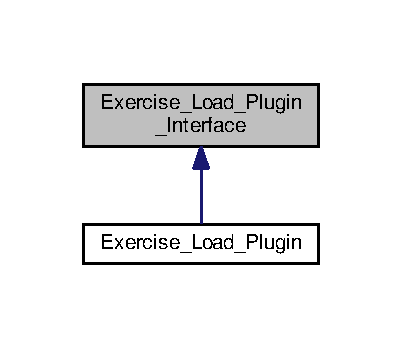
\includegraphics[width=193pt]{classExercise__Load__Plugin__Interface__inherit__graph}
\end{center}
\end{figure}
\subsection*{Signals}
\begin{DoxyCompactItemize}
\item 
virtual void \hyperlink{classExercise__Load__Plugin__Interface_a1672d1247efd8051607500adb4547ea1}{do\+\_\+post\+\_\+exercise} (Q\+Standard\+Item\+Model $\ast$)=0
\item 
virtual void \hyperlink{classExercise__Load__Plugin__Interface_a1672d1247efd8051607500adb4547ea1}{do\+\_\+post\+\_\+exercise} (Q\+Standard\+Item\+Model $\ast$)=0
\end{DoxyCompactItemize}
\subsection*{Public Member Functions}
\begin{DoxyCompactItemize}
\item 
virtual void \hyperlink{classExercise__Load__Plugin__Interface_abb9fef00080e48c6ce458b7476db97d9}{post\+\_\+exercise} (Q\+Standard\+Item\+Model $\ast$)=0
\item 
virtual Q\+String \hyperlink{classExercise__Load__Plugin__Interface_ab6899b947c3890e73b8a64b3c76c60de}{Name} () const =0
\item 
virtual void \hyperlink{classExercise__Load__Plugin__Interface_abb9fef00080e48c6ce458b7476db97d9}{post\+\_\+exercise} (Q\+Standard\+Item\+Model $\ast$)=0
\item 
virtual Q\+String \hyperlink{classExercise__Load__Plugin__Interface_ab6899b947c3890e73b8a64b3c76c60de}{Name} () const =0
\end{DoxyCompactItemize}


\subsection{Detailed Description}


Definition at line 7 of file excercise\+\_\+load\+\_\+plugin\+\_\+interface.\+h.



\subsection{Member Function Documentation}
\mbox{\Hypertarget{classExercise__Load__Plugin__Interface_a1672d1247efd8051607500adb4547ea1}\label{classExercise__Load__Plugin__Interface_a1672d1247efd8051607500adb4547ea1}} 
\index{Exercise\+\_\+\+Load\+\_\+\+Plugin\+\_\+\+Interface@{Exercise\+\_\+\+Load\+\_\+\+Plugin\+\_\+\+Interface}!do\+\_\+post\+\_\+exercise@{do\+\_\+post\+\_\+exercise}}
\index{do\+\_\+post\+\_\+exercise@{do\+\_\+post\+\_\+exercise}!Exercise\+\_\+\+Load\+\_\+\+Plugin\+\_\+\+Interface@{Exercise\+\_\+\+Load\+\_\+\+Plugin\+\_\+\+Interface}}
\subsubsection{\texorpdfstring{do\+\_\+post\+\_\+exercise}{do\_post\_exercise}\hspace{0.1cm}{\footnotesize\ttfamily [1/2]}}
{\footnotesize\ttfamily virtual void Exercise\+\_\+\+Load\+\_\+\+Plugin\+\_\+\+Interface\+::do\+\_\+post\+\_\+exercise (\begin{DoxyParamCaption}\item[{Q\+Standard\+Item\+Model $\ast$}]{ }\end{DoxyParamCaption})\hspace{0.3cm}{\ttfamily [pure virtual]}, {\ttfamily [signal]}}

\mbox{\Hypertarget{classExercise__Load__Plugin__Interface_a1672d1247efd8051607500adb4547ea1}\label{classExercise__Load__Plugin__Interface_a1672d1247efd8051607500adb4547ea1}} 
\index{Exercise\+\_\+\+Load\+\_\+\+Plugin\+\_\+\+Interface@{Exercise\+\_\+\+Load\+\_\+\+Plugin\+\_\+\+Interface}!do\+\_\+post\+\_\+exercise@{do\+\_\+post\+\_\+exercise}}
\index{do\+\_\+post\+\_\+exercise@{do\+\_\+post\+\_\+exercise}!Exercise\+\_\+\+Load\+\_\+\+Plugin\+\_\+\+Interface@{Exercise\+\_\+\+Load\+\_\+\+Plugin\+\_\+\+Interface}}
\subsubsection{\texorpdfstring{do\+\_\+post\+\_\+exercise}{do\_post\_exercise}\hspace{0.1cm}{\footnotesize\ttfamily [2/2]}}
{\footnotesize\ttfamily virtual void Exercise\+\_\+\+Load\+\_\+\+Plugin\+\_\+\+Interface\+::do\+\_\+post\+\_\+exercise (\begin{DoxyParamCaption}\item[{Q\+Standard\+Item\+Model $\ast$}]{ }\end{DoxyParamCaption})\hspace{0.3cm}{\ttfamily [pure virtual]}, {\ttfamily [signal]}}

\mbox{\Hypertarget{classExercise__Load__Plugin__Interface_ab6899b947c3890e73b8a64b3c76c60de}\label{classExercise__Load__Plugin__Interface_ab6899b947c3890e73b8a64b3c76c60de}} 
\index{Exercise\+\_\+\+Load\+\_\+\+Plugin\+\_\+\+Interface@{Exercise\+\_\+\+Load\+\_\+\+Plugin\+\_\+\+Interface}!Name@{Name}}
\index{Name@{Name}!Exercise\+\_\+\+Load\+\_\+\+Plugin\+\_\+\+Interface@{Exercise\+\_\+\+Load\+\_\+\+Plugin\+\_\+\+Interface}}
\subsubsection{\texorpdfstring{Name()}{Name()}\hspace{0.1cm}{\footnotesize\ttfamily [1/2]}}
{\footnotesize\ttfamily virtual Q\+String Exercise\+\_\+\+Load\+\_\+\+Plugin\+\_\+\+Interface\+::\+Name (\begin{DoxyParamCaption}{ }\end{DoxyParamCaption}) const\hspace{0.3cm}{\ttfamily [pure virtual]}}



Implemented in \hyperlink{classExercise__Load__Plugin_af6226d33bef2f1f526a8f37ec33e431c}{Exercise\+\_\+\+Load\+\_\+\+Plugin}.

Here is the caller graph for this function\+:\nopagebreak
\begin{figure}[H]
\begin{center}
\leavevmode
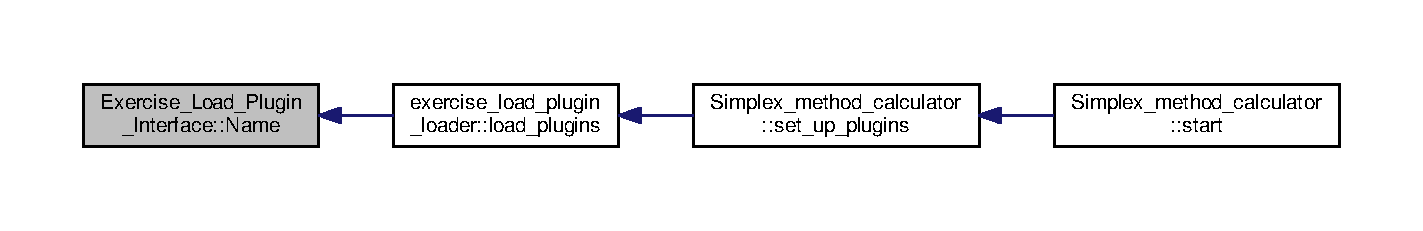
\includegraphics[width=350pt]{classExercise__Load__Plugin__Interface_ab6899b947c3890e73b8a64b3c76c60de_icgraph}
\end{center}
\end{figure}
\mbox{\Hypertarget{classExercise__Load__Plugin__Interface_ab6899b947c3890e73b8a64b3c76c60de}\label{classExercise__Load__Plugin__Interface_ab6899b947c3890e73b8a64b3c76c60de}} 
\index{Exercise\+\_\+\+Load\+\_\+\+Plugin\+\_\+\+Interface@{Exercise\+\_\+\+Load\+\_\+\+Plugin\+\_\+\+Interface}!Name@{Name}}
\index{Name@{Name}!Exercise\+\_\+\+Load\+\_\+\+Plugin\+\_\+\+Interface@{Exercise\+\_\+\+Load\+\_\+\+Plugin\+\_\+\+Interface}}
\subsubsection{\texorpdfstring{Name()}{Name()}\hspace{0.1cm}{\footnotesize\ttfamily [2/2]}}
{\footnotesize\ttfamily virtual Q\+String Exercise\+\_\+\+Load\+\_\+\+Plugin\+\_\+\+Interface\+::\+Name (\begin{DoxyParamCaption}{ }\end{DoxyParamCaption}) const\hspace{0.3cm}{\ttfamily [pure virtual]}}



Implemented in \hyperlink{classExercise__Load__Plugin_af6226d33bef2f1f526a8f37ec33e431c}{Exercise\+\_\+\+Load\+\_\+\+Plugin}.

\mbox{\Hypertarget{classExercise__Load__Plugin__Interface_abb9fef00080e48c6ce458b7476db97d9}\label{classExercise__Load__Plugin__Interface_abb9fef00080e48c6ce458b7476db97d9}} 
\index{Exercise\+\_\+\+Load\+\_\+\+Plugin\+\_\+\+Interface@{Exercise\+\_\+\+Load\+\_\+\+Plugin\+\_\+\+Interface}!post\+\_\+exercise@{post\+\_\+exercise}}
\index{post\+\_\+exercise@{post\+\_\+exercise}!Exercise\+\_\+\+Load\+\_\+\+Plugin\+\_\+\+Interface@{Exercise\+\_\+\+Load\+\_\+\+Plugin\+\_\+\+Interface}}
\subsubsection{\texorpdfstring{post\+\_\+exercise()}{post\_exercise()}\hspace{0.1cm}{\footnotesize\ttfamily [1/2]}}
{\footnotesize\ttfamily virtual void Exercise\+\_\+\+Load\+\_\+\+Plugin\+\_\+\+Interface\+::post\+\_\+exercise (\begin{DoxyParamCaption}\item[{Q\+Standard\+Item\+Model $\ast$}]{ }\end{DoxyParamCaption})\hspace{0.3cm}{\ttfamily [pure virtual]}}



Implemented in \hyperlink{classExercise__Load__Plugin_ad0c7c810dd492a014e17d40cdfe3d35d}{Exercise\+\_\+\+Load\+\_\+\+Plugin}.

Here is the caller graph for this function\+:\nopagebreak
\begin{figure}[H]
\begin{center}
\leavevmode
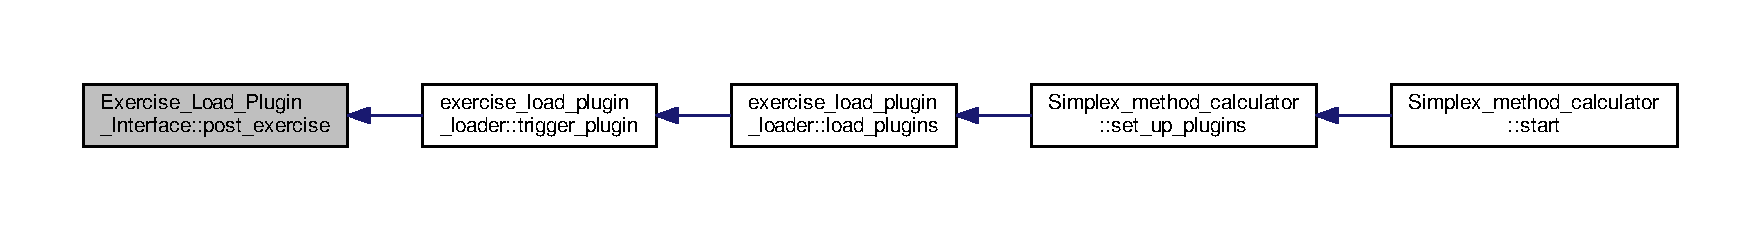
\includegraphics[width=350pt]{classExercise__Load__Plugin__Interface_abb9fef00080e48c6ce458b7476db97d9_icgraph}
\end{center}
\end{figure}
\mbox{\Hypertarget{classExercise__Load__Plugin__Interface_abb9fef00080e48c6ce458b7476db97d9}\label{classExercise__Load__Plugin__Interface_abb9fef00080e48c6ce458b7476db97d9}} 
\index{Exercise\+\_\+\+Load\+\_\+\+Plugin\+\_\+\+Interface@{Exercise\+\_\+\+Load\+\_\+\+Plugin\+\_\+\+Interface}!post\+\_\+exercise@{post\+\_\+exercise}}
\index{post\+\_\+exercise@{post\+\_\+exercise}!Exercise\+\_\+\+Load\+\_\+\+Plugin\+\_\+\+Interface@{Exercise\+\_\+\+Load\+\_\+\+Plugin\+\_\+\+Interface}}
\subsubsection{\texorpdfstring{post\+\_\+exercise()}{post\_exercise()}\hspace{0.1cm}{\footnotesize\ttfamily [2/2]}}
{\footnotesize\ttfamily virtual void Exercise\+\_\+\+Load\+\_\+\+Plugin\+\_\+\+Interface\+::post\+\_\+exercise (\begin{DoxyParamCaption}\item[{Q\+Standard\+Item\+Model $\ast$}]{ }\end{DoxyParamCaption})\hspace{0.3cm}{\ttfamily [pure virtual]}}



Implemented in \hyperlink{classExercise__Load__Plugin_ad0c7c810dd492a014e17d40cdfe3d35d}{Exercise\+\_\+\+Load\+\_\+\+Plugin}.



The documentation for this class was generated from the following file\+:\begin{DoxyCompactItemize}
\item 
Exercise\+\_\+\+Load\+\_\+\+Plugin/\hyperlink{Exercise__Load__Plugin_2excercise__load__plugin__interface_8h}{excercise\+\_\+load\+\_\+plugin\+\_\+interface.\+h}\end{DoxyCompactItemize}

\hypertarget{classexercise__load__plugin__loader}{}\section{exercise\+\_\+load\+\_\+plugin\+\_\+loader Class Reference}
\label{classexercise__load__plugin__loader}\index{exercise\+\_\+load\+\_\+plugin\+\_\+loader@{exercise\+\_\+load\+\_\+plugin\+\_\+loader}}


{\ttfamily \#include $<$exercise\+\_\+load\+\_\+plugin\+\_\+loader.\+h$>$}



Inherits Q\+Object.



Collaboration diagram for exercise\+\_\+load\+\_\+plugin\+\_\+loader\+:\nopagebreak
\begin{figure}[H]
\begin{center}
\leavevmode
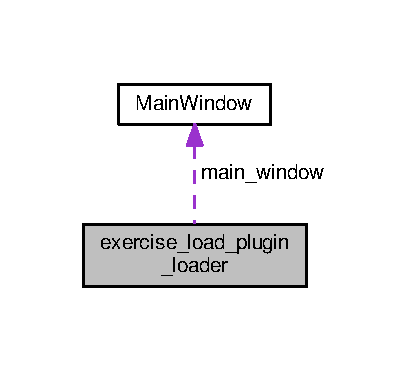
\includegraphics[width=197pt]{classexercise__load__plugin__loader__coll__graph}
\end{center}
\end{figure}
\subsection*{Public Slots}
\begin{DoxyCompactItemize}
\item 
void \hyperlink{classexercise__load__plugin__loader_a43ae5461bec5ad5a7afdb25a4ae2b021}{trigger\+\_\+plugin} (Q\+Action $\ast$menu\+\_\+action)
\end{DoxyCompactItemize}
\subsection*{Public Member Functions}
\begin{DoxyCompactItemize}
\item 
\hyperlink{classexercise__load__plugin__loader_a1c0b6c3d02cae87b2ef013267f6c1c95}{exercise\+\_\+load\+\_\+plugin\+\_\+loader} (Q\+Object $\ast$parent=nullptr, \hyperlink{classMainWindow}{Main\+Window} $\ast$w=nullptr)
\item 
void \hyperlink{classexercise__load__plugin__loader_a1a388b6c581a2fb5870f16913181284e}{load\+\_\+plugins} (Q\+Dir root\+\_\+dir)
\end{DoxyCompactItemize}
\subsection*{Private Attributes}
\begin{DoxyCompactItemize}
\item 
Q\+Object $\ast$ \hyperlink{classexercise__load__plugin__loader_adba0ee3eb5d4ed08e25b302a0cd33afa}{parent\+\_\+}
\item 
\hyperlink{classMainWindow}{Main\+Window} $\ast$ \hyperlink{classexercise__load__plugin__loader_a94b804f5276c83ac1877a161d012df6d}{main\+\_\+window}
\end{DoxyCompactItemize}


\subsection{Detailed Description}


Definition at line 14 of file exercise\+\_\+load\+\_\+plugin\+\_\+loader.\+h.



\subsection{Constructor \& Destructor Documentation}
\mbox{\Hypertarget{classexercise__load__plugin__loader_a1c0b6c3d02cae87b2ef013267f6c1c95}\label{classexercise__load__plugin__loader_a1c0b6c3d02cae87b2ef013267f6c1c95}} 
\index{exercise\+\_\+load\+\_\+plugin\+\_\+loader@{exercise\+\_\+load\+\_\+plugin\+\_\+loader}!exercise\+\_\+load\+\_\+plugin\+\_\+loader@{exercise\+\_\+load\+\_\+plugin\+\_\+loader}}
\index{exercise\+\_\+load\+\_\+plugin\+\_\+loader@{exercise\+\_\+load\+\_\+plugin\+\_\+loader}!exercise\+\_\+load\+\_\+plugin\+\_\+loader@{exercise\+\_\+load\+\_\+plugin\+\_\+loader}}
\subsubsection{\texorpdfstring{exercise\+\_\+load\+\_\+plugin\+\_\+loader()}{exercise\_load\_plugin\_loader()}}
{\footnotesize\ttfamily exercise\+\_\+load\+\_\+plugin\+\_\+loader\+::exercise\+\_\+load\+\_\+plugin\+\_\+loader (\begin{DoxyParamCaption}\item[{Q\+Object $\ast$}]{parent = {\ttfamily nullptr},  }\item[{\hyperlink{classMainWindow}{Main\+Window} $\ast$}]{w = {\ttfamily nullptr} }\end{DoxyParamCaption})\hspace{0.3cm}{\ttfamily [explicit]}}



Definition at line 3 of file exercise\+\_\+load\+\_\+plugin\+\_\+loader.\+cpp.



\subsection{Member Function Documentation}
\mbox{\Hypertarget{classexercise__load__plugin__loader_a1a388b6c581a2fb5870f16913181284e}\label{classexercise__load__plugin__loader_a1a388b6c581a2fb5870f16913181284e}} 
\index{exercise\+\_\+load\+\_\+plugin\+\_\+loader@{exercise\+\_\+load\+\_\+plugin\+\_\+loader}!load\+\_\+plugins@{load\+\_\+plugins}}
\index{load\+\_\+plugins@{load\+\_\+plugins}!exercise\+\_\+load\+\_\+plugin\+\_\+loader@{exercise\+\_\+load\+\_\+plugin\+\_\+loader}}
\subsubsection{\texorpdfstring{load\+\_\+plugins()}{load\_plugins()}}
{\footnotesize\ttfamily void exercise\+\_\+load\+\_\+plugin\+\_\+loader\+::load\+\_\+plugins (\begin{DoxyParamCaption}\item[{Q\+Dir}]{root\+\_\+dir }\end{DoxyParamCaption})}



Definition at line 8 of file exercise\+\_\+load\+\_\+plugin\+\_\+loader.\+cpp.

Here is the call graph for this function\+:\nopagebreak
\begin{figure}[H]
\begin{center}
\leavevmode
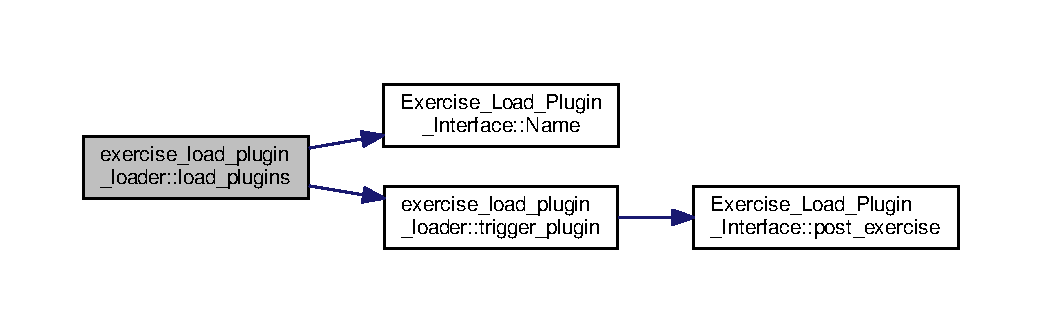
\includegraphics[width=350pt]{classexercise__load__plugin__loader_a1a388b6c581a2fb5870f16913181284e_cgraph}
\end{center}
\end{figure}
Here is the caller graph for this function\+:\nopagebreak
\begin{figure}[H]
\begin{center}
\leavevmode
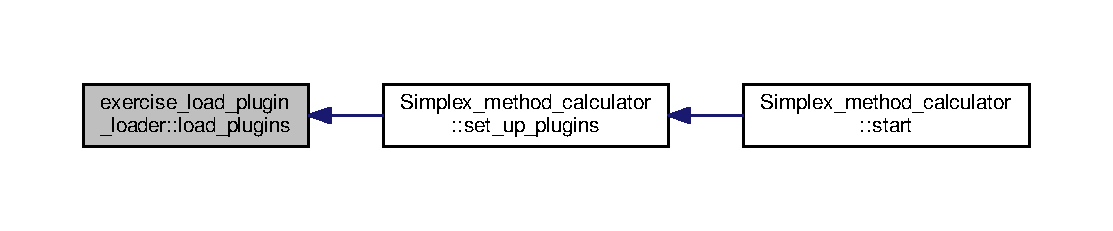
\includegraphics[width=350pt]{classexercise__load__plugin__loader_a1a388b6c581a2fb5870f16913181284e_icgraph}
\end{center}
\end{figure}
\mbox{\Hypertarget{classexercise__load__plugin__loader_a43ae5461bec5ad5a7afdb25a4ae2b021}\label{classexercise__load__plugin__loader_a43ae5461bec5ad5a7afdb25a4ae2b021}} 
\index{exercise\+\_\+load\+\_\+plugin\+\_\+loader@{exercise\+\_\+load\+\_\+plugin\+\_\+loader}!trigger\+\_\+plugin@{trigger\+\_\+plugin}}
\index{trigger\+\_\+plugin@{trigger\+\_\+plugin}!exercise\+\_\+load\+\_\+plugin\+\_\+loader@{exercise\+\_\+load\+\_\+plugin\+\_\+loader}}
\subsubsection{\texorpdfstring{trigger\+\_\+plugin}{trigger\_plugin}}
{\footnotesize\ttfamily void exercise\+\_\+load\+\_\+plugin\+\_\+loader\+::trigger\+\_\+plugin (\begin{DoxyParamCaption}\item[{Q\+Action $\ast$}]{menu\+\_\+action }\end{DoxyParamCaption})\hspace{0.3cm}{\ttfamily [slot]}}



Definition at line 36 of file exercise\+\_\+load\+\_\+plugin\+\_\+loader.\+cpp.

Here is the call graph for this function\+:\nopagebreak
\begin{figure}[H]
\begin{center}
\leavevmode
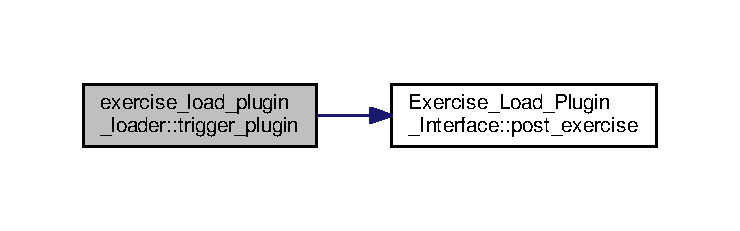
\includegraphics[width=350pt]{classexercise__load__plugin__loader_a43ae5461bec5ad5a7afdb25a4ae2b021_cgraph}
\end{center}
\end{figure}
Here is the caller graph for this function\+:\nopagebreak
\begin{figure}[H]
\begin{center}
\leavevmode
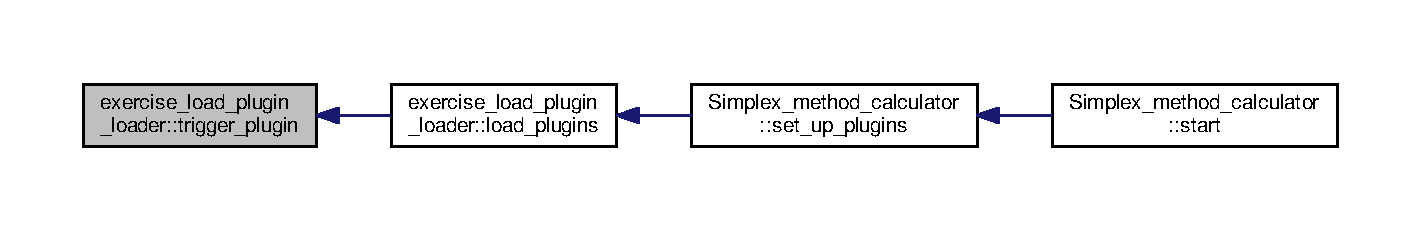
\includegraphics[width=350pt]{classexercise__load__plugin__loader_a43ae5461bec5ad5a7afdb25a4ae2b021_icgraph}
\end{center}
\end{figure}


\subsection{Member Data Documentation}
\mbox{\Hypertarget{classexercise__load__plugin__loader_a94b804f5276c83ac1877a161d012df6d}\label{classexercise__load__plugin__loader_a94b804f5276c83ac1877a161d012df6d}} 
\index{exercise\+\_\+load\+\_\+plugin\+\_\+loader@{exercise\+\_\+load\+\_\+plugin\+\_\+loader}!main\+\_\+window@{main\+\_\+window}}
\index{main\+\_\+window@{main\+\_\+window}!exercise\+\_\+load\+\_\+plugin\+\_\+loader@{exercise\+\_\+load\+\_\+plugin\+\_\+loader}}
\subsubsection{\texorpdfstring{main\+\_\+window}{main\_window}}
{\footnotesize\ttfamily \hyperlink{classMainWindow}{Main\+Window}$\ast$ exercise\+\_\+load\+\_\+plugin\+\_\+loader\+::main\+\_\+window\hspace{0.3cm}{\ttfamily [private]}}



Definition at line 23 of file exercise\+\_\+load\+\_\+plugin\+\_\+loader.\+h.

\mbox{\Hypertarget{classexercise__load__plugin__loader_adba0ee3eb5d4ed08e25b302a0cd33afa}\label{classexercise__load__plugin__loader_adba0ee3eb5d4ed08e25b302a0cd33afa}} 
\index{exercise\+\_\+load\+\_\+plugin\+\_\+loader@{exercise\+\_\+load\+\_\+plugin\+\_\+loader}!parent\+\_\+@{parent\+\_\+}}
\index{parent\+\_\+@{parent\+\_\+}!exercise\+\_\+load\+\_\+plugin\+\_\+loader@{exercise\+\_\+load\+\_\+plugin\+\_\+loader}}
\subsubsection{\texorpdfstring{parent\+\_\+}{parent\_}}
{\footnotesize\ttfamily Q\+Object$\ast$ exercise\+\_\+load\+\_\+plugin\+\_\+loader\+::parent\+\_\+\hspace{0.3cm}{\ttfamily [private]}}



Definition at line 22 of file exercise\+\_\+load\+\_\+plugin\+\_\+loader.\+h.



The documentation for this class was generated from the following files\+:\begin{DoxyCompactItemize}
\item 
simplex\+\_\+app/\hyperlink{exercise__load__plugin__loader_8h}{exercise\+\_\+load\+\_\+plugin\+\_\+loader.\+h}\item 
simplex\+\_\+app/\hyperlink{exercise__load__plugin__loader_8cpp}{exercise\+\_\+load\+\_\+plugin\+\_\+loader.\+cpp}\end{DoxyCompactItemize}

\hypertarget{classgui__plugin__loader}{}\section{gui\+\_\+plugin\+\_\+loader Class Reference}
\label{classgui__plugin__loader}\index{gui\+\_\+plugin\+\_\+loader@{gui\+\_\+plugin\+\_\+loader}}


{\ttfamily \#include $<$gui\+\_\+plugin\+\_\+loader.\+h$>$}



Inherits Q\+Object.



Collaboration diagram for gui\+\_\+plugin\+\_\+loader\+:\nopagebreak
\begin{figure}[H]
\begin{center}
\leavevmode
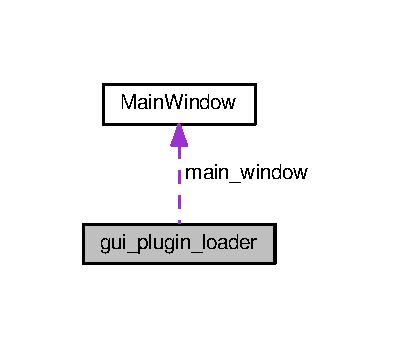
\includegraphics[width=189pt]{classgui__plugin__loader__coll__graph}
\end{center}
\end{figure}
\subsection*{Public Slots}
\begin{DoxyCompactItemize}
\item 
void \hyperlink{classgui__plugin__loader_a0d2c0ab3d2eefbc2b6dcc246ea58d43b}{set\+\_\+gui} (Q\+Action $\ast$menuitem)
\end{DoxyCompactItemize}
\subsection*{Public Member Functions}
\begin{DoxyCompactItemize}
\item 
\hyperlink{classgui__plugin__loader_a06e6c9395877425822e5f178804962f3}{gui\+\_\+plugin\+\_\+loader} (Q\+Object $\ast$parent=nullptr, \hyperlink{classMainWindow}{Main\+Window} $\ast$w=nullptr)
\item 
void \hyperlink{classgui__plugin__loader_afaea2c8da605ce9ee8e2995449a67eda}{load\+\_\+plugins} (Q\+Dir root\+\_\+dir)
\end{DoxyCompactItemize}
\subsection*{Private Member Functions}
\begin{DoxyCompactItemize}
\item 
void \hyperlink{classgui__plugin__loader_a41f08e87c06edd90551177c9d26e20b6}{emit\+\_\+signals\+\_\+to\+\_\+set\+\_\+models\+\_\+of\+\_\+views} ()
\item 
void \hyperlink{classgui__plugin__loader_a1aa2e332cd05954fcb9bbf506450c290}{emit\+\_\+signals\+\_\+to\+\_\+set\+\_\+delegates} ()
\end{DoxyCompactItemize}
\subsection*{Private Attributes}
\begin{DoxyCompactItemize}
\item 
Q\+Object $\ast$ \hyperlink{classgui__plugin__loader_a6bf4626d341c427f2c72a8b504dd2086}{parent\+\_\+}
\item 
\hyperlink{classMainWindow}{Main\+Window} $\ast$ \hyperlink{classgui__plugin__loader_a1ff765127327eec72360c355a6255642}{main\+\_\+window}
\end{DoxyCompactItemize}
\subsection*{Friends}
\begin{DoxyCompactItemize}
\item 
class \hyperlink{classgui__plugin__loader_aa57bcac61e09f9c999a2f048dc923409}{Simplex\+\_\+method\+\_\+calculator}
\end{DoxyCompactItemize}


\subsection{Detailed Description}


Definition at line 14 of file gui\+\_\+plugin\+\_\+loader.\+h.



\subsection{Constructor \& Destructor Documentation}
\mbox{\Hypertarget{classgui__plugin__loader_a06e6c9395877425822e5f178804962f3}\label{classgui__plugin__loader_a06e6c9395877425822e5f178804962f3}} 
\index{gui\+\_\+plugin\+\_\+loader@{gui\+\_\+plugin\+\_\+loader}!gui\+\_\+plugin\+\_\+loader@{gui\+\_\+plugin\+\_\+loader}}
\index{gui\+\_\+plugin\+\_\+loader@{gui\+\_\+plugin\+\_\+loader}!gui\+\_\+plugin\+\_\+loader@{gui\+\_\+plugin\+\_\+loader}}
\subsubsection{\texorpdfstring{gui\+\_\+plugin\+\_\+loader()}{gui\_plugin\_loader()}}
{\footnotesize\ttfamily gui\+\_\+plugin\+\_\+loader\+::gui\+\_\+plugin\+\_\+loader (\begin{DoxyParamCaption}\item[{Q\+Object $\ast$}]{parent = {\ttfamily nullptr},  }\item[{\hyperlink{classMainWindow}{Main\+Window} $\ast$}]{w = {\ttfamily nullptr} }\end{DoxyParamCaption})\hspace{0.3cm}{\ttfamily [explicit]}}



Definition at line 9 of file gui\+\_\+plugin\+\_\+loader.\+cpp.



\subsection{Member Function Documentation}
\mbox{\Hypertarget{classgui__plugin__loader_a1aa2e332cd05954fcb9bbf506450c290}\label{classgui__plugin__loader_a1aa2e332cd05954fcb9bbf506450c290}} 
\index{gui\+\_\+plugin\+\_\+loader@{gui\+\_\+plugin\+\_\+loader}!emit\+\_\+signals\+\_\+to\+\_\+set\+\_\+delegates@{emit\+\_\+signals\+\_\+to\+\_\+set\+\_\+delegates}}
\index{emit\+\_\+signals\+\_\+to\+\_\+set\+\_\+delegates@{emit\+\_\+signals\+\_\+to\+\_\+set\+\_\+delegates}!gui\+\_\+plugin\+\_\+loader@{gui\+\_\+plugin\+\_\+loader}}
\subsubsection{\texorpdfstring{emit\+\_\+signals\+\_\+to\+\_\+set\+\_\+delegates()}{emit\_signals\_to\_set\_delegates()}}
{\footnotesize\ttfamily void gui\+\_\+plugin\+\_\+loader\+::emit\+\_\+signals\+\_\+to\+\_\+set\+\_\+delegates (\begin{DoxyParamCaption}{ }\end{DoxyParamCaption})\hspace{0.3cm}{\ttfamily [private]}}



Definition at line 95 of file gui\+\_\+plugin\+\_\+loader.\+cpp.

Here is the caller graph for this function\+:\nopagebreak
\begin{figure}[H]
\begin{center}
\leavevmode
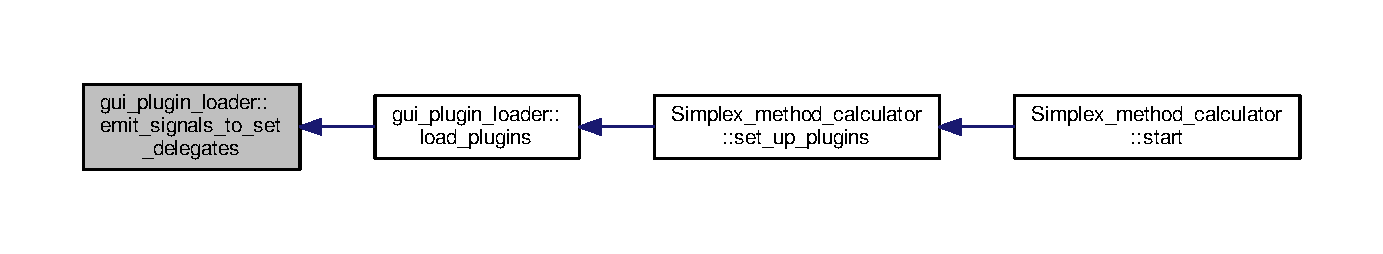
\includegraphics[width=350pt]{classgui__plugin__loader_a1aa2e332cd05954fcb9bbf506450c290_icgraph}
\end{center}
\end{figure}
\mbox{\Hypertarget{classgui__plugin__loader_a41f08e87c06edd90551177c9d26e20b6}\label{classgui__plugin__loader_a41f08e87c06edd90551177c9d26e20b6}} 
\index{gui\+\_\+plugin\+\_\+loader@{gui\+\_\+plugin\+\_\+loader}!emit\+\_\+signals\+\_\+to\+\_\+set\+\_\+models\+\_\+of\+\_\+views@{emit\+\_\+signals\+\_\+to\+\_\+set\+\_\+models\+\_\+of\+\_\+views}}
\index{emit\+\_\+signals\+\_\+to\+\_\+set\+\_\+models\+\_\+of\+\_\+views@{emit\+\_\+signals\+\_\+to\+\_\+set\+\_\+models\+\_\+of\+\_\+views}!gui\+\_\+plugin\+\_\+loader@{gui\+\_\+plugin\+\_\+loader}}
\subsubsection{\texorpdfstring{emit\+\_\+signals\+\_\+to\+\_\+set\+\_\+models\+\_\+of\+\_\+views()}{emit\_signals\_to\_set\_models\_of\_views()}}
{\footnotesize\ttfamily void gui\+\_\+plugin\+\_\+loader\+::emit\+\_\+signals\+\_\+to\+\_\+set\+\_\+models\+\_\+of\+\_\+views (\begin{DoxyParamCaption}{ }\end{DoxyParamCaption})\hspace{0.3cm}{\ttfamily [private]}}



Definition at line 85 of file gui\+\_\+plugin\+\_\+loader.\+cpp.

Here is the caller graph for this function\+:\nopagebreak
\begin{figure}[H]
\begin{center}
\leavevmode
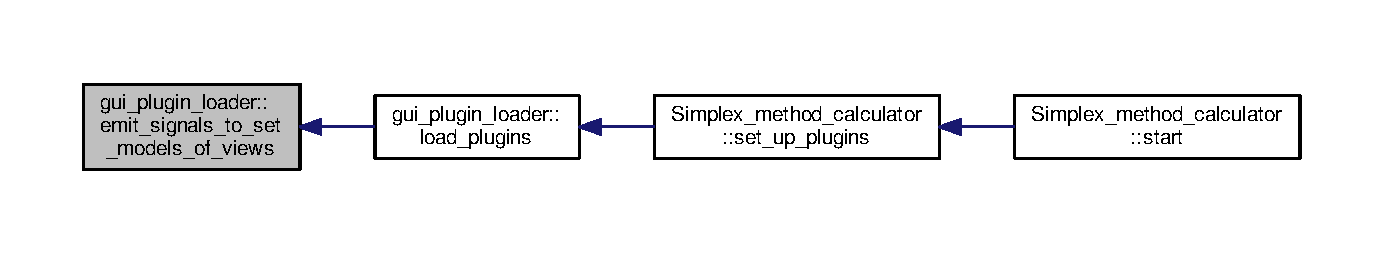
\includegraphics[width=350pt]{classgui__plugin__loader_a41f08e87c06edd90551177c9d26e20b6_icgraph}
\end{center}
\end{figure}
\mbox{\Hypertarget{classgui__plugin__loader_afaea2c8da605ce9ee8e2995449a67eda}\label{classgui__plugin__loader_afaea2c8da605ce9ee8e2995449a67eda}} 
\index{gui\+\_\+plugin\+\_\+loader@{gui\+\_\+plugin\+\_\+loader}!load\+\_\+plugins@{load\+\_\+plugins}}
\index{load\+\_\+plugins@{load\+\_\+plugins}!gui\+\_\+plugin\+\_\+loader@{gui\+\_\+plugin\+\_\+loader}}
\subsubsection{\texorpdfstring{load\+\_\+plugins()}{load\_plugins()}}
{\footnotesize\ttfamily void gui\+\_\+plugin\+\_\+loader\+::load\+\_\+plugins (\begin{DoxyParamCaption}\item[{Q\+Dir}]{root\+\_\+dir }\end{DoxyParamCaption})}



Definition at line 15 of file gui\+\_\+plugin\+\_\+loader.\+cpp.

Here is the call graph for this function\+:\nopagebreak
\begin{figure}[H]
\begin{center}
\leavevmode
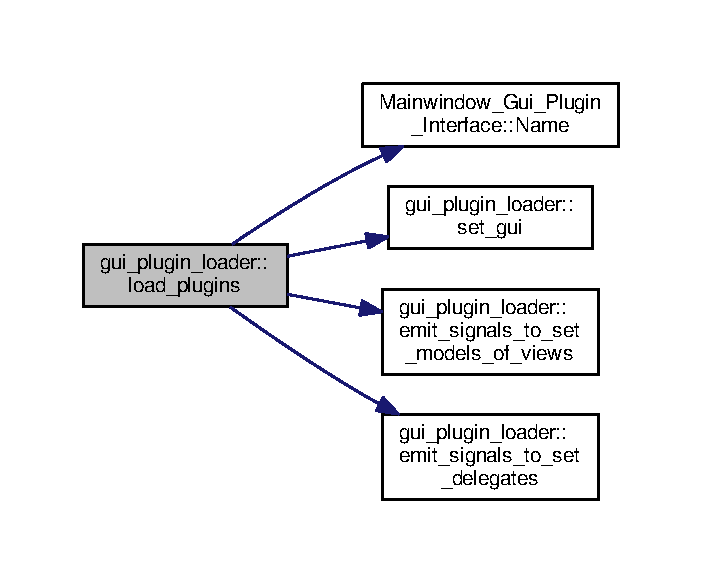
\includegraphics[width=337pt]{classgui__plugin__loader_afaea2c8da605ce9ee8e2995449a67eda_cgraph}
\end{center}
\end{figure}
Here is the caller graph for this function\+:\nopagebreak
\begin{figure}[H]
\begin{center}
\leavevmode
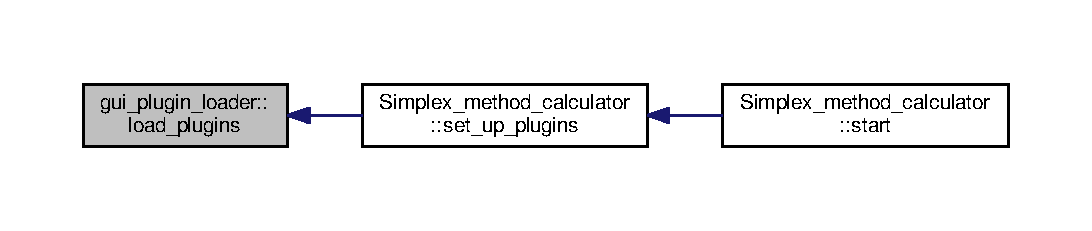
\includegraphics[width=350pt]{classgui__plugin__loader_afaea2c8da605ce9ee8e2995449a67eda_icgraph}
\end{center}
\end{figure}
\mbox{\Hypertarget{classgui__plugin__loader_a0d2c0ab3d2eefbc2b6dcc246ea58d43b}\label{classgui__plugin__loader_a0d2c0ab3d2eefbc2b6dcc246ea58d43b}} 
\index{gui\+\_\+plugin\+\_\+loader@{gui\+\_\+plugin\+\_\+loader}!set\+\_\+gui@{set\+\_\+gui}}
\index{set\+\_\+gui@{set\+\_\+gui}!gui\+\_\+plugin\+\_\+loader@{gui\+\_\+plugin\+\_\+loader}}
\subsubsection{\texorpdfstring{set\+\_\+gui}{set\_gui}}
{\footnotesize\ttfamily void gui\+\_\+plugin\+\_\+loader\+::set\+\_\+gui (\begin{DoxyParamCaption}\item[{Q\+Action $\ast$}]{menuitem }\end{DoxyParamCaption})\hspace{0.3cm}{\ttfamily [slot]}}



Definition at line 78 of file gui\+\_\+plugin\+\_\+loader.\+cpp.

Here is the caller graph for this function\+:\nopagebreak
\begin{figure}[H]
\begin{center}
\leavevmode
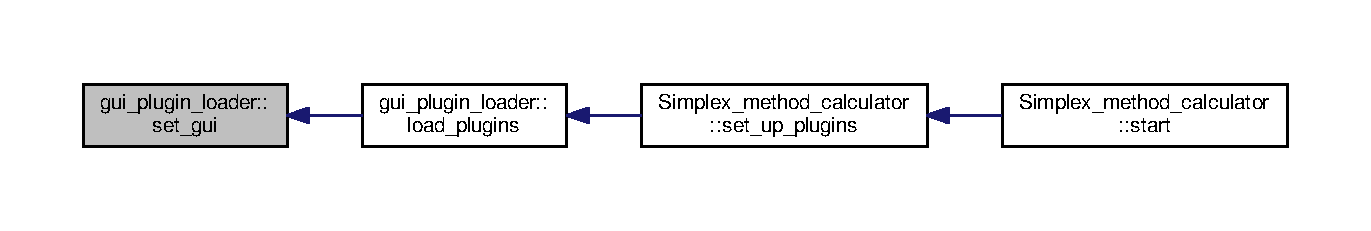
\includegraphics[width=350pt]{classgui__plugin__loader_a0d2c0ab3d2eefbc2b6dcc246ea58d43b_icgraph}
\end{center}
\end{figure}


\subsection{Friends And Related Function Documentation}
\mbox{\Hypertarget{classgui__plugin__loader_aa57bcac61e09f9c999a2f048dc923409}\label{classgui__plugin__loader_aa57bcac61e09f9c999a2f048dc923409}} 
\index{gui\+\_\+plugin\+\_\+loader@{gui\+\_\+plugin\+\_\+loader}!Simplex\+\_\+method\+\_\+calculator@{Simplex\+\_\+method\+\_\+calculator}}
\index{Simplex\+\_\+method\+\_\+calculator@{Simplex\+\_\+method\+\_\+calculator}!gui\+\_\+plugin\+\_\+loader@{gui\+\_\+plugin\+\_\+loader}}
\subsubsection{\texorpdfstring{Simplex\+\_\+method\+\_\+calculator}{Simplex\_method\_calculator}}
{\footnotesize\ttfamily friend class \hyperlink{classSimplex__method__calculator}{Simplex\+\_\+method\+\_\+calculator}\hspace{0.3cm}{\ttfamily [friend]}}



Definition at line 17 of file gui\+\_\+plugin\+\_\+loader.\+h.



\subsection{Member Data Documentation}
\mbox{\Hypertarget{classgui__plugin__loader_a1ff765127327eec72360c355a6255642}\label{classgui__plugin__loader_a1ff765127327eec72360c355a6255642}} 
\index{gui\+\_\+plugin\+\_\+loader@{gui\+\_\+plugin\+\_\+loader}!main\+\_\+window@{main\+\_\+window}}
\index{main\+\_\+window@{main\+\_\+window}!gui\+\_\+plugin\+\_\+loader@{gui\+\_\+plugin\+\_\+loader}}
\subsubsection{\texorpdfstring{main\+\_\+window}{main\_window}}
{\footnotesize\ttfamily \hyperlink{classMainWindow}{Main\+Window}$\ast$ gui\+\_\+plugin\+\_\+loader\+::main\+\_\+window\hspace{0.3cm}{\ttfamily [private]}}



Definition at line 33 of file gui\+\_\+plugin\+\_\+loader.\+h.

\mbox{\Hypertarget{classgui__plugin__loader_a6bf4626d341c427f2c72a8b504dd2086}\label{classgui__plugin__loader_a6bf4626d341c427f2c72a8b504dd2086}} 
\index{gui\+\_\+plugin\+\_\+loader@{gui\+\_\+plugin\+\_\+loader}!parent\+\_\+@{parent\+\_\+}}
\index{parent\+\_\+@{parent\+\_\+}!gui\+\_\+plugin\+\_\+loader@{gui\+\_\+plugin\+\_\+loader}}
\subsubsection{\texorpdfstring{parent\+\_\+}{parent\_}}
{\footnotesize\ttfamily Q\+Object$\ast$ gui\+\_\+plugin\+\_\+loader\+::parent\+\_\+\hspace{0.3cm}{\ttfamily [private]}}



Definition at line 32 of file gui\+\_\+plugin\+\_\+loader.\+h.



The documentation for this class was generated from the following files\+:\begin{DoxyCompactItemize}
\item 
simplex\+\_\+app/\hyperlink{gui__plugin__loader_8h}{gui\+\_\+plugin\+\_\+loader.\+h}\item 
simplex\+\_\+app/\hyperlink{gui__plugin__loader_8cpp}{gui\+\_\+plugin\+\_\+loader.\+cpp}\end{DoxyCompactItemize}

\hypertarget{classMainvindow__gui__plugin}{}\section{Mainvindow\+\_\+gui\+\_\+plugin Class Reference}
\label{classMainvindow__gui__plugin}\index{Mainvindow\+\_\+gui\+\_\+plugin@{Mainvindow\+\_\+gui\+\_\+plugin}}


{\ttfamily \#include $<$mainvindow\+\_\+gui\+\_\+plugin.\+h$>$}



Inheritance diagram for Mainvindow\+\_\+gui\+\_\+plugin\+:\nopagebreak
\begin{figure}[H]
\begin{center}
\leavevmode
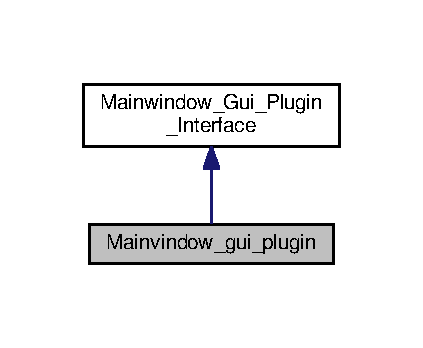
\includegraphics[width=203pt]{classMainvindow__gui__plugin__inherit__graph}
\end{center}
\end{figure}


Collaboration diagram for Mainvindow\+\_\+gui\+\_\+plugin\+:\nopagebreak
\begin{figure}[H]
\begin{center}
\leavevmode
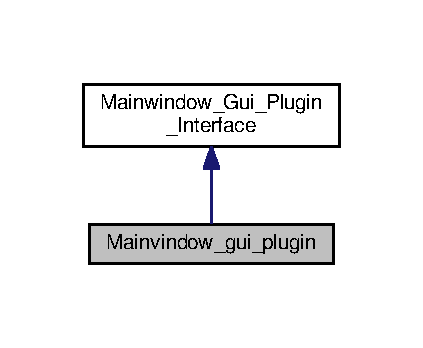
\includegraphics[width=203pt]{classMainvindow__gui__plugin__coll__graph}
\end{center}
\end{figure}
\subsection*{Public Slots}
\begin{DoxyCompactItemize}
\item 
void \hyperlink{classMainvindow__gui__plugin_a51be893d4ce6d2f88269b7c5de29dee1}{do\+\_\+set\+\_\+indulo\+\_\+model\+\_\+view} (Q\+Standard\+Item\+Model $\ast$) Q\+\_\+\+D\+E\+C\+L\+\_\+\+O\+V\+E\+R\+R\+I\+DE
\item 
void \hyperlink{classMainvindow__gui__plugin_a57e149b56d9cb9f0084c859fe4dfbc4b}{do\+\_\+set\+\_\+kanonikus\+\_\+alak\+\_\+model\+\_\+view} (Q\+Standard\+Item\+Model $\ast$) Q\+\_\+\+D\+E\+C\+L\+\_\+\+O\+V\+E\+R\+R\+I\+DE
\item 
void \hyperlink{classMainvindow__gui__plugin_a4be633148117ee9541d59733cd591dd7}{do\+\_\+set\+\_\+indulo\+\_\+matrix\+\_\+model\+\_\+view} (Q\+Standard\+Item\+Model $\ast$) Q\+\_\+\+D\+E\+C\+L\+\_\+\+O\+V\+E\+R\+R\+I\+DE
\item 
void \hyperlink{classMainvindow__gui__plugin_ad86b393bdcb1266fc78ad579c4fb22f8}{do\+\_\+set\+\_\+utolso\+\_\+elotti\+\_\+allapot\+\_\+model\+\_\+view} (Q\+Standard\+Item\+Model $\ast$) Q\+\_\+\+D\+E\+C\+L\+\_\+\+O\+V\+E\+R\+R\+I\+DE
\item 
void \hyperlink{classMainvindow__gui__plugin_a501eff78dd74f522383650aa90612d74}{do\+\_\+set\+\_\+utolso\+\_\+allapot\+\_\+model\+\_\+view} (Q\+Standard\+Item\+Model $\ast$) Q\+\_\+\+D\+E\+C\+L\+\_\+\+O\+V\+E\+R\+R\+I\+DE
\item 
void \hyperlink{classMainvindow__gui__plugin_ade84b9f3aabf1a82847eccc5ca868e15}{do\+\_\+when\+\_\+indulo\+\_\+feladat\+\_\+changed} () Q\+\_\+\+D\+E\+C\+L\+\_\+\+O\+V\+E\+R\+R\+I\+DE
\item 
void \hyperlink{classMainvindow__gui__plugin_a2c147430a48369193b3ac08128aca977}{do\+\_\+when\+\_\+vegigszamol\+\_\+changed} (bool checked) Q\+\_\+\+D\+E\+C\+L\+\_\+\+O\+V\+E\+R\+R\+I\+DE
\item 
void \hyperlink{classMainvindow__gui__plugin_a4ad9ff7c5361c013b272505503c21acb}{do\+\_\+when\+\_\+external\+\_\+exercise\+\_\+loaded} (int termtenyezo, int korl\+\_\+felt) Q\+\_\+\+D\+E\+C\+L\+\_\+\+O\+V\+E\+R\+R\+I\+DE
\item 
void \hyperlink{classMainvindow__gui__plugin_a144bcf420ee4a90d79eac642ffd66c54}{do\+\_\+when\+\_\+got\+\_\+kanonikus\+\_\+clicked} () Q\+\_\+\+D\+E\+C\+L\+\_\+\+O\+V\+E\+R\+R\+I\+DE
\item 
void \hyperlink{classMainvindow__gui__plugin_a1b835b4de00749d30479b17c58452c13}{do\+\_\+when\+\_\+got\+\_\+indulo\+\_\+matrix\+\_\+clicked} () Q\+\_\+\+D\+E\+C\+L\+\_\+\+O\+V\+E\+R\+R\+I\+DE
\item 
void \hyperlink{classMainvindow__gui__plugin_aaf24d376b70a136b52e8dae5dfc3ad15}{do\+\_\+set\+\_\+delegate\+\_\+for\+\_\+numbers} (Q\+Styled\+Item\+Delegate $\ast$delegate) Q\+\_\+\+D\+E\+C\+L\+\_\+\+O\+V\+E\+R\+R\+I\+DE
\begin{DoxyCompactList}\small\item\em A fő program altal biztosított numerikus delegátor beállítása. \end{DoxyCompactList}\item 
void \hyperlink{classMainvindow__gui__plugin_a7f8f250d9d8b2adc3ee04b768f9b3ee8}{do\+\_\+set\+\_\+non\+\_\+numeric\+\_\+delegate} (Q\+Item\+Delegate $\ast$delegate) Q\+\_\+\+D\+E\+C\+L\+\_\+\+O\+V\+E\+R\+R\+I\+DE
\begin{DoxyCompactList}\small\item\em A fő program altal biztosított nem-\/numerikus delegátor beállítása. \end{DoxyCompactList}\item 
void \hyperlink{classMainvindow__gui__plugin_a8134d2856b60ba95754aa899c39bbabe}{do\+\_\+when\+\_\+button\+\_\+kezd\+\_\+clicked} (int termteny, int korlfelt) Q\+\_\+\+D\+E\+C\+L\+\_\+\+O\+V\+E\+R\+R\+I\+DE
\end{DoxyCompactItemize}
\subsection*{Signals}
\begin{DoxyCompactItemize}
\item 
void \hyperlink{classMainvindow__gui__plugin_adb6c0d468163f8192f2138b15a6c43e9}{sor\+\_\+oszlop\+\_\+db} (int, int) Q\+\_\+\+D\+E\+C\+L\+\_\+\+F\+I\+N\+AL
\item 
void \hyperlink{classMainvindow__gui__plugin_ab72edb0176103371d01ede7a001746a4}{make\+\_\+kanonikus} () Q\+\_\+\+D\+E\+C\+L\+\_\+\+F\+I\+N\+AL
\item 
void \hyperlink{classMainvindow__gui__plugin_ae1b472871fd6e98296a968a1f6dee653}{make\+\_\+indulo\+\_\+matrix} () Q\+\_\+\+D\+E\+C\+L\+\_\+\+F\+I\+N\+AL
\item 
void \hyperlink{classMainvindow__gui__plugin_ae7b7382ef0b52b1116426d3fc9c78caa}{szamol} () Q\+\_\+\+D\+E\+C\+L\+\_\+\+F\+I\+N\+AL
\item 
void \hyperlink{classMainvindow__gui__plugin_a2fe7a4a60ee4e4f61579ccc717e8258d}{vegigszamol} (bool vegigszamolando) Q\+\_\+\+D\+E\+C\+L\+\_\+\+F\+I\+N\+AL
\item 
void \hyperlink{classMainvindow__gui__plugin_aacc5de871594914c5d4c8edcec6576a8}{kanonikus\+\_\+clicked} () Q\+\_\+\+D\+E\+C\+L\+\_\+\+F\+I\+N\+AL
\item 
void \hyperlink{classMainvindow__gui__plugin_a9f1289a2d061b153834961a41e442a35}{indulo\+\_\+matrix\+\_\+clicked} () Q\+\_\+\+D\+E\+C\+L\+\_\+\+F\+I\+N\+AL
\end{DoxyCompactItemize}
\subsection*{Public Member Functions}
\begin{DoxyCompactItemize}
\item 
\hyperlink{classMainvindow__gui__plugin_afed5eb76ea21523ae97a36ed11d82b3f}{Mainvindow\+\_\+gui\+\_\+plugin} (Q\+Widget $\ast$parent=nullptr)
\item 
\hyperlink{classMainvindow__gui__plugin_a17a7101b7163acaa42f8026292d0a672}{$\sim$\+Mainvindow\+\_\+gui\+\_\+plugin} () override
\item 
Q\+String \hyperlink{classMainvindow__gui__plugin_affd8ce27d7e94a2adac287bc8dd835e0}{Name} () const override
\end{DoxyCompactItemize}
\subsection*{Private Slots}
\begin{DoxyCompactItemize}
\item 
void \hyperlink{classMainvindow__gui__plugin_af96459b75bff1299029ed450753b7c62}{on\+\_\+button\+\_\+szamol\+\_\+clicked} ()
\item 
void \hyperlink{classMainvindow__gui__plugin_a5d703f8eb1cc3a327861f0bc4f2e3439}{on\+\_\+button\+\_\+indulo\+\_\+matrix\+\_\+clicked} ()
\item 
void \hyperlink{classMainvindow__gui__plugin_a5c3a19e9e7e6cbe8a6f6fc16c88e16b4}{on\+\_\+button\+\_\+kezd\+\_\+clicked} ()
\item 
void \hyperlink{classMainvindow__gui__plugin_aa6705f09c4288a6bc9f5a08a995d3789}{on\+\_\+button\+\_\+kanonikus\+\_\+clicked} ()
\item 
void \hyperlink{classMainvindow__gui__plugin_a2dd76229829de1230f2f12928131d397}{on\+\_\+radio\+Button\+\_\+2\+\_\+toggled} (bool checked)
\item 
void \hyperlink{classMainvindow__gui__plugin_a7e06d5ee7068a413da91bb8125ad4a7d}{on\+\_\+radio\+Button\+\_\+toggled} (bool checked)
\end{DoxyCompactItemize}
\subsection*{Private Attributes}
\begin{DoxyCompactItemize}
\item 
Ui\+::\+Mainvindow\+\_\+gui\+\_\+plugin $\ast$ \hyperlink{classMainvindow__gui__plugin_a86399ba5cca2bb2ab811afc6dd47ccc8}{ui}
\item 
Q\+Styled\+Item\+Delegate $\ast$ \hyperlink{classMainvindow__gui__plugin_a1ae497c20498fc8347d6d8c7691a4220}{number\+\_\+delegator}
\item 
Q\+Item\+Delegate $\ast$ \hyperlink{classMainvindow__gui__plugin_adabe60e85b8b8dedc41da660506595a1}{non\+\_\+numeric\+\_\+delegate}
\end{DoxyCompactItemize}


\subsection{Detailed Description}


Definition at line 16 of file mainvindow\+\_\+gui\+\_\+plugin.\+h.



\subsection{Constructor \& Destructor Documentation}
\mbox{\Hypertarget{classMainvindow__gui__plugin_afed5eb76ea21523ae97a36ed11d82b3f}\label{classMainvindow__gui__plugin_afed5eb76ea21523ae97a36ed11d82b3f}} 
\index{Mainvindow\+\_\+gui\+\_\+plugin@{Mainvindow\+\_\+gui\+\_\+plugin}!Mainvindow\+\_\+gui\+\_\+plugin@{Mainvindow\+\_\+gui\+\_\+plugin}}
\index{Mainvindow\+\_\+gui\+\_\+plugin@{Mainvindow\+\_\+gui\+\_\+plugin}!Mainvindow\+\_\+gui\+\_\+plugin@{Mainvindow\+\_\+gui\+\_\+plugin}}
\subsubsection{\texorpdfstring{Mainvindow\+\_\+gui\+\_\+plugin()}{Mainvindow\_gui\_plugin()}}
{\footnotesize\ttfamily Mainvindow\+\_\+gui\+\_\+plugin\+::\+Mainvindow\+\_\+gui\+\_\+plugin (\begin{DoxyParamCaption}\item[{Q\+Widget $\ast$}]{parent = {\ttfamily nullptr} }\end{DoxyParamCaption})\hspace{0.3cm}{\ttfamily [explicit]}}



Definition at line 4 of file mainvindow\+\_\+gui\+\_\+plugin.\+cpp.

\mbox{\Hypertarget{classMainvindow__gui__plugin_a17a7101b7163acaa42f8026292d0a672}\label{classMainvindow__gui__plugin_a17a7101b7163acaa42f8026292d0a672}} 
\index{Mainvindow\+\_\+gui\+\_\+plugin@{Mainvindow\+\_\+gui\+\_\+plugin}!````~Mainvindow\+\_\+gui\+\_\+plugin@{$\sim$\+Mainvindow\+\_\+gui\+\_\+plugin}}
\index{````~Mainvindow\+\_\+gui\+\_\+plugin@{$\sim$\+Mainvindow\+\_\+gui\+\_\+plugin}!Mainvindow\+\_\+gui\+\_\+plugin@{Mainvindow\+\_\+gui\+\_\+plugin}}
\subsubsection{\texorpdfstring{$\sim$\+Mainvindow\+\_\+gui\+\_\+plugin()}{~Mainvindow\_gui\_plugin()}}
{\footnotesize\ttfamily Mainvindow\+\_\+gui\+\_\+plugin\+::$\sim$\+Mainvindow\+\_\+gui\+\_\+plugin (\begin{DoxyParamCaption}{ }\end{DoxyParamCaption})\hspace{0.3cm}{\ttfamily [override]}}



Definition at line 20 of file mainvindow\+\_\+gui\+\_\+plugin.\+cpp.



\subsection{Member Function Documentation}
\mbox{\Hypertarget{classMainvindow__gui__plugin_aaf24d376b70a136b52e8dae5dfc3ad15}\label{classMainvindow__gui__plugin_aaf24d376b70a136b52e8dae5dfc3ad15}} 
\index{Mainvindow\+\_\+gui\+\_\+plugin@{Mainvindow\+\_\+gui\+\_\+plugin}!do\+\_\+set\+\_\+delegate\+\_\+for\+\_\+numbers@{do\+\_\+set\+\_\+delegate\+\_\+for\+\_\+numbers}}
\index{do\+\_\+set\+\_\+delegate\+\_\+for\+\_\+numbers@{do\+\_\+set\+\_\+delegate\+\_\+for\+\_\+numbers}!Mainvindow\+\_\+gui\+\_\+plugin@{Mainvindow\+\_\+gui\+\_\+plugin}}
\subsubsection{\texorpdfstring{do\+\_\+set\+\_\+delegate\+\_\+for\+\_\+numbers}{do\_set\_delegate\_for\_numbers}}
{\footnotesize\ttfamily void Mainvindow\+\_\+gui\+\_\+plugin\+::do\+\_\+set\+\_\+delegate\+\_\+for\+\_\+numbers (\begin{DoxyParamCaption}\item[{Q\+Styled\+Item\+Delegate $\ast$}]{delegate }\end{DoxyParamCaption})\hspace{0.3cm}{\ttfamily [slot]}}



A fő program altal biztosított numerikus delegátor beállítása. 

A fő program biztosít agy alap delegátort a numerikus adatoknak. Ebben az osztályban ezt használjuk numerikus delegátornak.


\begin{DoxyParams}{Parameters}
{\em delegate} & A főprogram által biztosított numerikus delegátorra mutató pointer. \\
\hline
\end{DoxyParams}


Definition at line 173 of file mainvindow\+\_\+gui\+\_\+plugin.\+cpp.

\mbox{\Hypertarget{classMainvindow__gui__plugin_a4be633148117ee9541d59733cd591dd7}\label{classMainvindow__gui__plugin_a4be633148117ee9541d59733cd591dd7}} 
\index{Mainvindow\+\_\+gui\+\_\+plugin@{Mainvindow\+\_\+gui\+\_\+plugin}!do\+\_\+set\+\_\+indulo\+\_\+matrix\+\_\+model\+\_\+view@{do\+\_\+set\+\_\+indulo\+\_\+matrix\+\_\+model\+\_\+view}}
\index{do\+\_\+set\+\_\+indulo\+\_\+matrix\+\_\+model\+\_\+view@{do\+\_\+set\+\_\+indulo\+\_\+matrix\+\_\+model\+\_\+view}!Mainvindow\+\_\+gui\+\_\+plugin@{Mainvindow\+\_\+gui\+\_\+plugin}}
\subsubsection{\texorpdfstring{do\+\_\+set\+\_\+indulo\+\_\+matrix\+\_\+model\+\_\+view}{do\_set\_indulo\_matrix\_model\_view}}
{\footnotesize\ttfamily void Mainvindow\+\_\+gui\+\_\+plugin\+::do\+\_\+set\+\_\+indulo\+\_\+matrix\+\_\+model\+\_\+view (\begin{DoxyParamCaption}\item[{Q\+Standard\+Item\+Model $\ast$}]{model }\end{DoxyParamCaption})\hspace{0.3cm}{\ttfamily [slot]}}



Definition at line 35 of file mainvindow\+\_\+gui\+\_\+plugin.\+cpp.

\mbox{\Hypertarget{classMainvindow__gui__plugin_a51be893d4ce6d2f88269b7c5de29dee1}\label{classMainvindow__gui__plugin_a51be893d4ce6d2f88269b7c5de29dee1}} 
\index{Mainvindow\+\_\+gui\+\_\+plugin@{Mainvindow\+\_\+gui\+\_\+plugin}!do\+\_\+set\+\_\+indulo\+\_\+model\+\_\+view@{do\+\_\+set\+\_\+indulo\+\_\+model\+\_\+view}}
\index{do\+\_\+set\+\_\+indulo\+\_\+model\+\_\+view@{do\+\_\+set\+\_\+indulo\+\_\+model\+\_\+view}!Mainvindow\+\_\+gui\+\_\+plugin@{Mainvindow\+\_\+gui\+\_\+plugin}}
\subsubsection{\texorpdfstring{do\+\_\+set\+\_\+indulo\+\_\+model\+\_\+view}{do\_set\_indulo\_model\_view}}
{\footnotesize\ttfamily void Mainvindow\+\_\+gui\+\_\+plugin\+::do\+\_\+set\+\_\+indulo\+\_\+model\+\_\+view (\begin{DoxyParamCaption}\item[{Q\+Standard\+Item\+Model $\ast$}]{model }\end{DoxyParamCaption})\hspace{0.3cm}{\ttfamily [slot]}}



Definition at line 24 of file mainvindow\+\_\+gui\+\_\+plugin.\+cpp.

\mbox{\Hypertarget{classMainvindow__gui__plugin_a57e149b56d9cb9f0084c859fe4dfbc4b}\label{classMainvindow__gui__plugin_a57e149b56d9cb9f0084c859fe4dfbc4b}} 
\index{Mainvindow\+\_\+gui\+\_\+plugin@{Mainvindow\+\_\+gui\+\_\+plugin}!do\+\_\+set\+\_\+kanonikus\+\_\+alak\+\_\+model\+\_\+view@{do\+\_\+set\+\_\+kanonikus\+\_\+alak\+\_\+model\+\_\+view}}
\index{do\+\_\+set\+\_\+kanonikus\+\_\+alak\+\_\+model\+\_\+view@{do\+\_\+set\+\_\+kanonikus\+\_\+alak\+\_\+model\+\_\+view}!Mainvindow\+\_\+gui\+\_\+plugin@{Mainvindow\+\_\+gui\+\_\+plugin}}
\subsubsection{\texorpdfstring{do\+\_\+set\+\_\+kanonikus\+\_\+alak\+\_\+model\+\_\+view}{do\_set\_kanonikus\_alak\_model\_view}}
{\footnotesize\ttfamily void Mainvindow\+\_\+gui\+\_\+plugin\+::do\+\_\+set\+\_\+kanonikus\+\_\+alak\+\_\+model\+\_\+view (\begin{DoxyParamCaption}\item[{Q\+Standard\+Item\+Model $\ast$}]{model }\end{DoxyParamCaption})\hspace{0.3cm}{\ttfamily [slot]}}



Definition at line 31 of file mainvindow\+\_\+gui\+\_\+plugin.\+cpp.

\mbox{\Hypertarget{classMainvindow__gui__plugin_a7f8f250d9d8b2adc3ee04b768f9b3ee8}\label{classMainvindow__gui__plugin_a7f8f250d9d8b2adc3ee04b768f9b3ee8}} 
\index{Mainvindow\+\_\+gui\+\_\+plugin@{Mainvindow\+\_\+gui\+\_\+plugin}!do\+\_\+set\+\_\+non\+\_\+numeric\+\_\+delegate@{do\+\_\+set\+\_\+non\+\_\+numeric\+\_\+delegate}}
\index{do\+\_\+set\+\_\+non\+\_\+numeric\+\_\+delegate@{do\+\_\+set\+\_\+non\+\_\+numeric\+\_\+delegate}!Mainvindow\+\_\+gui\+\_\+plugin@{Mainvindow\+\_\+gui\+\_\+plugin}}
\subsubsection{\texorpdfstring{do\+\_\+set\+\_\+non\+\_\+numeric\+\_\+delegate}{do\_set\_non\_numeric\_delegate}}
{\footnotesize\ttfamily void Mainvindow\+\_\+gui\+\_\+plugin\+::do\+\_\+set\+\_\+non\+\_\+numeric\+\_\+delegate (\begin{DoxyParamCaption}\item[{Q\+Item\+Delegate $\ast$}]{delegate }\end{DoxyParamCaption})\hspace{0.3cm}{\ttfamily [slot]}}



A fő program altal biztosított nem-\/numerikus delegátor beállítása. 

A fő program biztosít agy alap delegátort a nem-\/numerikus adatoknak. Ebben az osztályban ezt használjuk nem-\/numerikus delegátornak.


\begin{DoxyParams}{Parameters}
{\em delegate} & A főprogram által biztosított nem-\/numerikus delegátorra mutató pointer. \\
\hline
\end{DoxyParams}


Definition at line 188 of file mainvindow\+\_\+gui\+\_\+plugin.\+cpp.

\mbox{\Hypertarget{classMainvindow__gui__plugin_a501eff78dd74f522383650aa90612d74}\label{classMainvindow__gui__plugin_a501eff78dd74f522383650aa90612d74}} 
\index{Mainvindow\+\_\+gui\+\_\+plugin@{Mainvindow\+\_\+gui\+\_\+plugin}!do\+\_\+set\+\_\+utolso\+\_\+allapot\+\_\+model\+\_\+view@{do\+\_\+set\+\_\+utolso\+\_\+allapot\+\_\+model\+\_\+view}}
\index{do\+\_\+set\+\_\+utolso\+\_\+allapot\+\_\+model\+\_\+view@{do\+\_\+set\+\_\+utolso\+\_\+allapot\+\_\+model\+\_\+view}!Mainvindow\+\_\+gui\+\_\+plugin@{Mainvindow\+\_\+gui\+\_\+plugin}}
\subsubsection{\texorpdfstring{do\+\_\+set\+\_\+utolso\+\_\+allapot\+\_\+model\+\_\+view}{do\_set\_utolso\_allapot\_model\_view}}
{\footnotesize\ttfamily void Mainvindow\+\_\+gui\+\_\+plugin\+::do\+\_\+set\+\_\+utolso\+\_\+allapot\+\_\+model\+\_\+view (\begin{DoxyParamCaption}\item[{Q\+Standard\+Item\+Model $\ast$}]{model }\end{DoxyParamCaption})\hspace{0.3cm}{\ttfamily [slot]}}



Definition at line 49 of file mainvindow\+\_\+gui\+\_\+plugin.\+cpp.

\mbox{\Hypertarget{classMainvindow__gui__plugin_ad86b393bdcb1266fc78ad579c4fb22f8}\label{classMainvindow__gui__plugin_ad86b393bdcb1266fc78ad579c4fb22f8}} 
\index{Mainvindow\+\_\+gui\+\_\+plugin@{Mainvindow\+\_\+gui\+\_\+plugin}!do\+\_\+set\+\_\+utolso\+\_\+elotti\+\_\+allapot\+\_\+model\+\_\+view@{do\+\_\+set\+\_\+utolso\+\_\+elotti\+\_\+allapot\+\_\+model\+\_\+view}}
\index{do\+\_\+set\+\_\+utolso\+\_\+elotti\+\_\+allapot\+\_\+model\+\_\+view@{do\+\_\+set\+\_\+utolso\+\_\+elotti\+\_\+allapot\+\_\+model\+\_\+view}!Mainvindow\+\_\+gui\+\_\+plugin@{Mainvindow\+\_\+gui\+\_\+plugin}}
\subsubsection{\texorpdfstring{do\+\_\+set\+\_\+utolso\+\_\+elotti\+\_\+allapot\+\_\+model\+\_\+view}{do\_set\_utolso\_elotti\_allapot\_model\_view}}
{\footnotesize\ttfamily void Mainvindow\+\_\+gui\+\_\+plugin\+::do\+\_\+set\+\_\+utolso\+\_\+elotti\+\_\+allapot\+\_\+model\+\_\+view (\begin{DoxyParamCaption}\item[{Q\+Standard\+Item\+Model $\ast$}]{model }\end{DoxyParamCaption})\hspace{0.3cm}{\ttfamily [slot]}}



Definition at line 42 of file mainvindow\+\_\+gui\+\_\+plugin.\+cpp.

\mbox{\Hypertarget{classMainvindow__gui__plugin_a8134d2856b60ba95754aa899c39bbabe}\label{classMainvindow__gui__plugin_a8134d2856b60ba95754aa899c39bbabe}} 
\index{Mainvindow\+\_\+gui\+\_\+plugin@{Mainvindow\+\_\+gui\+\_\+plugin}!do\+\_\+when\+\_\+button\+\_\+kezd\+\_\+clicked@{do\+\_\+when\+\_\+button\+\_\+kezd\+\_\+clicked}}
\index{do\+\_\+when\+\_\+button\+\_\+kezd\+\_\+clicked@{do\+\_\+when\+\_\+button\+\_\+kezd\+\_\+clicked}!Mainvindow\+\_\+gui\+\_\+plugin@{Mainvindow\+\_\+gui\+\_\+plugin}}
\subsubsection{\texorpdfstring{do\+\_\+when\+\_\+button\+\_\+kezd\+\_\+clicked}{do\_when\_button\_kezd\_clicked}}
{\footnotesize\ttfamily void Mainvindow\+\_\+gui\+\_\+plugin\+::do\+\_\+when\+\_\+button\+\_\+kezd\+\_\+clicked (\begin{DoxyParamCaption}\item[{int}]{termteny,  }\item[{int}]{korlfelt }\end{DoxyParamCaption})\hspace{0.3cm}{\ttfamily [slot]}}



Definition at line 90 of file mainvindow\+\_\+gui\+\_\+plugin.\+cpp.

\mbox{\Hypertarget{classMainvindow__gui__plugin_a4ad9ff7c5361c013b272505503c21acb}\label{classMainvindow__gui__plugin_a4ad9ff7c5361c013b272505503c21acb}} 
\index{Mainvindow\+\_\+gui\+\_\+plugin@{Mainvindow\+\_\+gui\+\_\+plugin}!do\+\_\+when\+\_\+external\+\_\+exercise\+\_\+loaded@{do\+\_\+when\+\_\+external\+\_\+exercise\+\_\+loaded}}
\index{do\+\_\+when\+\_\+external\+\_\+exercise\+\_\+loaded@{do\+\_\+when\+\_\+external\+\_\+exercise\+\_\+loaded}!Mainvindow\+\_\+gui\+\_\+plugin@{Mainvindow\+\_\+gui\+\_\+plugin}}
\subsubsection{\texorpdfstring{do\+\_\+when\+\_\+external\+\_\+exercise\+\_\+loaded}{do\_when\_external\_exercise\_loaded}}
{\footnotesize\ttfamily void Mainvindow\+\_\+gui\+\_\+plugin\+::do\+\_\+when\+\_\+external\+\_\+exercise\+\_\+loaded (\begin{DoxyParamCaption}\item[{int}]{termtenyezo,  }\item[{int}]{korl\+\_\+felt }\end{DoxyParamCaption})\hspace{0.3cm}{\ttfamily [slot]}}



Definition at line 147 of file mainvindow\+\_\+gui\+\_\+plugin.\+cpp.

\mbox{\Hypertarget{classMainvindow__gui__plugin_a1b835b4de00749d30479b17c58452c13}\label{classMainvindow__gui__plugin_a1b835b4de00749d30479b17c58452c13}} 
\index{Mainvindow\+\_\+gui\+\_\+plugin@{Mainvindow\+\_\+gui\+\_\+plugin}!do\+\_\+when\+\_\+got\+\_\+indulo\+\_\+matrix\+\_\+clicked@{do\+\_\+when\+\_\+got\+\_\+indulo\+\_\+matrix\+\_\+clicked}}
\index{do\+\_\+when\+\_\+got\+\_\+indulo\+\_\+matrix\+\_\+clicked@{do\+\_\+when\+\_\+got\+\_\+indulo\+\_\+matrix\+\_\+clicked}!Mainvindow\+\_\+gui\+\_\+plugin@{Mainvindow\+\_\+gui\+\_\+plugin}}
\subsubsection{\texorpdfstring{do\+\_\+when\+\_\+got\+\_\+indulo\+\_\+matrix\+\_\+clicked}{do\_when\_got\_indulo\_matrix\_clicked}}
{\footnotesize\ttfamily void Mainvindow\+\_\+gui\+\_\+plugin\+::do\+\_\+when\+\_\+got\+\_\+indulo\+\_\+matrix\+\_\+clicked (\begin{DoxyParamCaption}{ }\end{DoxyParamCaption})\hspace{0.3cm}{\ttfamily [slot]}}



Definition at line 76 of file mainvindow\+\_\+gui\+\_\+plugin.\+cpp.

\mbox{\Hypertarget{classMainvindow__gui__plugin_a144bcf420ee4a90d79eac642ffd66c54}\label{classMainvindow__gui__plugin_a144bcf420ee4a90d79eac642ffd66c54}} 
\index{Mainvindow\+\_\+gui\+\_\+plugin@{Mainvindow\+\_\+gui\+\_\+plugin}!do\+\_\+when\+\_\+got\+\_\+kanonikus\+\_\+clicked@{do\+\_\+when\+\_\+got\+\_\+kanonikus\+\_\+clicked}}
\index{do\+\_\+when\+\_\+got\+\_\+kanonikus\+\_\+clicked@{do\+\_\+when\+\_\+got\+\_\+kanonikus\+\_\+clicked}!Mainvindow\+\_\+gui\+\_\+plugin@{Mainvindow\+\_\+gui\+\_\+plugin}}
\subsubsection{\texorpdfstring{do\+\_\+when\+\_\+got\+\_\+kanonikus\+\_\+clicked}{do\_when\_got\_kanonikus\_clicked}}
{\footnotesize\ttfamily void Mainvindow\+\_\+gui\+\_\+plugin\+::do\+\_\+when\+\_\+got\+\_\+kanonikus\+\_\+clicked (\begin{DoxyParamCaption}{ }\end{DoxyParamCaption})\hspace{0.3cm}{\ttfamily [slot]}}



Definition at line 114 of file mainvindow\+\_\+gui\+\_\+plugin.\+cpp.

\mbox{\Hypertarget{classMainvindow__gui__plugin_ade84b9f3aabf1a82847eccc5ca868e15}\label{classMainvindow__gui__plugin_ade84b9f3aabf1a82847eccc5ca868e15}} 
\index{Mainvindow\+\_\+gui\+\_\+plugin@{Mainvindow\+\_\+gui\+\_\+plugin}!do\+\_\+when\+\_\+indulo\+\_\+feladat\+\_\+changed@{do\+\_\+when\+\_\+indulo\+\_\+feladat\+\_\+changed}}
\index{do\+\_\+when\+\_\+indulo\+\_\+feladat\+\_\+changed@{do\+\_\+when\+\_\+indulo\+\_\+feladat\+\_\+changed}!Mainvindow\+\_\+gui\+\_\+plugin@{Mainvindow\+\_\+gui\+\_\+plugin}}
\subsubsection{\texorpdfstring{do\+\_\+when\+\_\+indulo\+\_\+feladat\+\_\+changed}{do\_when\_indulo\_feladat\_changed}}
{\footnotesize\ttfamily void Mainvindow\+\_\+gui\+\_\+plugin\+::do\+\_\+when\+\_\+indulo\+\_\+feladat\+\_\+changed (\begin{DoxyParamCaption}{ }\end{DoxyParamCaption})\hspace{0.3cm}{\ttfamily [slot]}}



Definition at line 124 of file mainvindow\+\_\+gui\+\_\+plugin.\+cpp.

\mbox{\Hypertarget{classMainvindow__gui__plugin_a2c147430a48369193b3ac08128aca977}\label{classMainvindow__gui__plugin_a2c147430a48369193b3ac08128aca977}} 
\index{Mainvindow\+\_\+gui\+\_\+plugin@{Mainvindow\+\_\+gui\+\_\+plugin}!do\+\_\+when\+\_\+vegigszamol\+\_\+changed@{do\+\_\+when\+\_\+vegigszamol\+\_\+changed}}
\index{do\+\_\+when\+\_\+vegigszamol\+\_\+changed@{do\+\_\+when\+\_\+vegigszamol\+\_\+changed}!Mainvindow\+\_\+gui\+\_\+plugin@{Mainvindow\+\_\+gui\+\_\+plugin}}
\subsubsection{\texorpdfstring{do\+\_\+when\+\_\+vegigszamol\+\_\+changed}{do\_when\_vegigszamol\_changed}}
{\footnotesize\ttfamily void Mainvindow\+\_\+gui\+\_\+plugin\+::do\+\_\+when\+\_\+vegigszamol\+\_\+changed (\begin{DoxyParamCaption}\item[{bool}]{checked }\end{DoxyParamCaption})\hspace{0.3cm}{\ttfamily [slot]}}



Definition at line 136 of file mainvindow\+\_\+gui\+\_\+plugin.\+cpp.

\mbox{\Hypertarget{classMainvindow__gui__plugin_a9f1289a2d061b153834961a41e442a35}\label{classMainvindow__gui__plugin_a9f1289a2d061b153834961a41e442a35}} 
\index{Mainvindow\+\_\+gui\+\_\+plugin@{Mainvindow\+\_\+gui\+\_\+plugin}!indulo\+\_\+matrix\+\_\+clicked@{indulo\+\_\+matrix\+\_\+clicked}}
\index{indulo\+\_\+matrix\+\_\+clicked@{indulo\+\_\+matrix\+\_\+clicked}!Mainvindow\+\_\+gui\+\_\+plugin@{Mainvindow\+\_\+gui\+\_\+plugin}}
\subsubsection{\texorpdfstring{indulo\+\_\+matrix\+\_\+clicked}{indulo\_matrix\_clicked}}
{\footnotesize\ttfamily void Mainvindow\+\_\+gui\+\_\+plugin\+::indulo\+\_\+matrix\+\_\+clicked (\begin{DoxyParamCaption}{ }\end{DoxyParamCaption})\hspace{0.3cm}{\ttfamily [signal]}}

Here is the caller graph for this function\+:\nopagebreak
\begin{figure}[H]
\begin{center}
\leavevmode
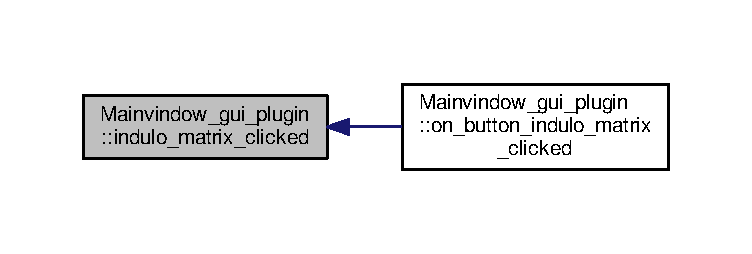
\includegraphics[width=350pt]{classMainvindow__gui__plugin_a9f1289a2d061b153834961a41e442a35_icgraph}
\end{center}
\end{figure}
\mbox{\Hypertarget{classMainvindow__gui__plugin_aacc5de871594914c5d4c8edcec6576a8}\label{classMainvindow__gui__plugin_aacc5de871594914c5d4c8edcec6576a8}} 
\index{Mainvindow\+\_\+gui\+\_\+plugin@{Mainvindow\+\_\+gui\+\_\+plugin}!kanonikus\+\_\+clicked@{kanonikus\+\_\+clicked}}
\index{kanonikus\+\_\+clicked@{kanonikus\+\_\+clicked}!Mainvindow\+\_\+gui\+\_\+plugin@{Mainvindow\+\_\+gui\+\_\+plugin}}
\subsubsection{\texorpdfstring{kanonikus\+\_\+clicked}{kanonikus\_clicked}}
{\footnotesize\ttfamily void Mainvindow\+\_\+gui\+\_\+plugin\+::kanonikus\+\_\+clicked (\begin{DoxyParamCaption}{ }\end{DoxyParamCaption})\hspace{0.3cm}{\ttfamily [signal]}}

Here is the caller graph for this function\+:\nopagebreak
\begin{figure}[H]
\begin{center}
\leavevmode
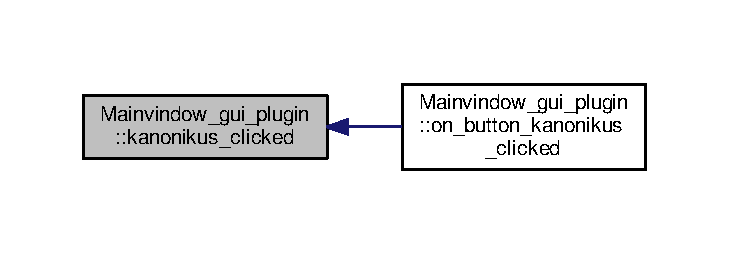
\includegraphics[width=350pt]{classMainvindow__gui__plugin_aacc5de871594914c5d4c8edcec6576a8_icgraph}
\end{center}
\end{figure}
\mbox{\Hypertarget{classMainvindow__gui__plugin_ae1b472871fd6e98296a968a1f6dee653}\label{classMainvindow__gui__plugin_ae1b472871fd6e98296a968a1f6dee653}} 
\index{Mainvindow\+\_\+gui\+\_\+plugin@{Mainvindow\+\_\+gui\+\_\+plugin}!make\+\_\+indulo\+\_\+matrix@{make\+\_\+indulo\+\_\+matrix}}
\index{make\+\_\+indulo\+\_\+matrix@{make\+\_\+indulo\+\_\+matrix}!Mainvindow\+\_\+gui\+\_\+plugin@{Mainvindow\+\_\+gui\+\_\+plugin}}
\subsubsection{\texorpdfstring{make\+\_\+indulo\+\_\+matrix}{make\_indulo\_matrix}}
{\footnotesize\ttfamily void Mainvindow\+\_\+gui\+\_\+plugin\+::make\+\_\+indulo\+\_\+matrix (\begin{DoxyParamCaption}{ }\end{DoxyParamCaption})\hspace{0.3cm}{\ttfamily [signal]}}

Here is the caller graph for this function\+:\nopagebreak
\begin{figure}[H]
\begin{center}
\leavevmode
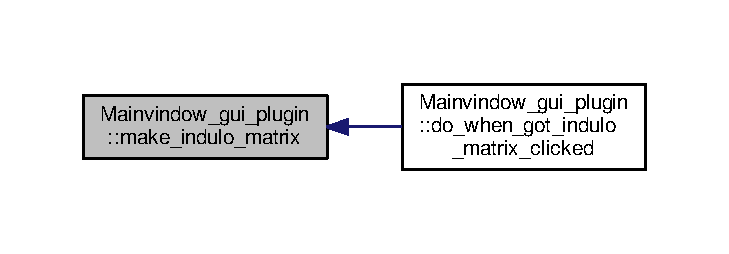
\includegraphics[width=350pt]{classMainvindow__gui__plugin_ae1b472871fd6e98296a968a1f6dee653_icgraph}
\end{center}
\end{figure}
\mbox{\Hypertarget{classMainvindow__gui__plugin_ab72edb0176103371d01ede7a001746a4}\label{classMainvindow__gui__plugin_ab72edb0176103371d01ede7a001746a4}} 
\index{Mainvindow\+\_\+gui\+\_\+plugin@{Mainvindow\+\_\+gui\+\_\+plugin}!make\+\_\+kanonikus@{make\+\_\+kanonikus}}
\index{make\+\_\+kanonikus@{make\+\_\+kanonikus}!Mainvindow\+\_\+gui\+\_\+plugin@{Mainvindow\+\_\+gui\+\_\+plugin}}
\subsubsection{\texorpdfstring{make\+\_\+kanonikus}{make\_kanonikus}}
{\footnotesize\ttfamily void Mainvindow\+\_\+gui\+\_\+plugin\+::make\+\_\+kanonikus (\begin{DoxyParamCaption}{ }\end{DoxyParamCaption})\hspace{0.3cm}{\ttfamily [signal]}}

Here is the caller graph for this function\+:\nopagebreak
\begin{figure}[H]
\begin{center}
\leavevmode
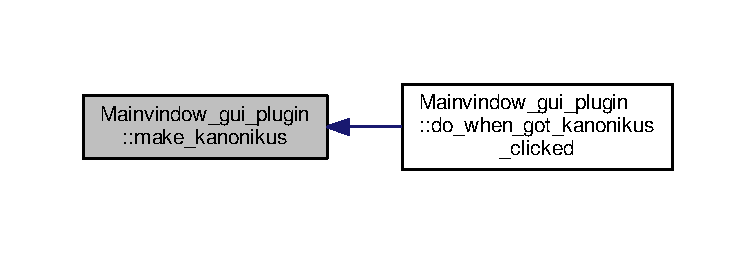
\includegraphics[width=350pt]{classMainvindow__gui__plugin_ab72edb0176103371d01ede7a001746a4_icgraph}
\end{center}
\end{figure}
\mbox{\Hypertarget{classMainvindow__gui__plugin_affd8ce27d7e94a2adac287bc8dd835e0}\label{classMainvindow__gui__plugin_affd8ce27d7e94a2adac287bc8dd835e0}} 
\index{Mainvindow\+\_\+gui\+\_\+plugin@{Mainvindow\+\_\+gui\+\_\+plugin}!Name@{Name}}
\index{Name@{Name}!Mainvindow\+\_\+gui\+\_\+plugin@{Mainvindow\+\_\+gui\+\_\+plugin}}
\subsubsection{\texorpdfstring{Name()}{Name()}}
{\footnotesize\ttfamily Q\+String Mainvindow\+\_\+gui\+\_\+plugin\+::\+Name (\begin{DoxyParamCaption}{ }\end{DoxyParamCaption}) const\hspace{0.3cm}{\ttfamily [override]}, {\ttfamily [virtual]}}



Implements \hyperlink{classMainwindow__Gui__Plugin__Interface_a5cbc7bb0e3bb477472b91f65e916db8e}{Mainwindow\+\_\+\+Gui\+\_\+\+Plugin\+\_\+\+Interface}.



Definition at line 56 of file mainvindow\+\_\+gui\+\_\+plugin.\+cpp.

\mbox{\Hypertarget{classMainvindow__gui__plugin_a5d703f8eb1cc3a327861f0bc4f2e3439}\label{classMainvindow__gui__plugin_a5d703f8eb1cc3a327861f0bc4f2e3439}} 
\index{Mainvindow\+\_\+gui\+\_\+plugin@{Mainvindow\+\_\+gui\+\_\+plugin}!on\+\_\+button\+\_\+indulo\+\_\+matrix\+\_\+clicked@{on\+\_\+button\+\_\+indulo\+\_\+matrix\+\_\+clicked}}
\index{on\+\_\+button\+\_\+indulo\+\_\+matrix\+\_\+clicked@{on\+\_\+button\+\_\+indulo\+\_\+matrix\+\_\+clicked}!Mainvindow\+\_\+gui\+\_\+plugin@{Mainvindow\+\_\+gui\+\_\+plugin}}
\subsubsection{\texorpdfstring{on\+\_\+button\+\_\+indulo\+\_\+matrix\+\_\+clicked}{on\_button\_indulo\_matrix\_clicked}}
{\footnotesize\ttfamily void Mainvindow\+\_\+gui\+\_\+plugin\+::on\+\_\+button\+\_\+indulo\+\_\+matrix\+\_\+clicked (\begin{DoxyParamCaption}{ }\end{DoxyParamCaption})\hspace{0.3cm}{\ttfamily [private]}, {\ttfamily [slot]}}



Definition at line 70 of file mainvindow\+\_\+gui\+\_\+plugin.\+cpp.

\mbox{\Hypertarget{classMainvindow__gui__plugin_aa6705f09c4288a6bc9f5a08a995d3789}\label{classMainvindow__gui__plugin_aa6705f09c4288a6bc9f5a08a995d3789}} 
\index{Mainvindow\+\_\+gui\+\_\+plugin@{Mainvindow\+\_\+gui\+\_\+plugin}!on\+\_\+button\+\_\+kanonikus\+\_\+clicked@{on\+\_\+button\+\_\+kanonikus\+\_\+clicked}}
\index{on\+\_\+button\+\_\+kanonikus\+\_\+clicked@{on\+\_\+button\+\_\+kanonikus\+\_\+clicked}!Mainvindow\+\_\+gui\+\_\+plugin@{Mainvindow\+\_\+gui\+\_\+plugin}}
\subsubsection{\texorpdfstring{on\+\_\+button\+\_\+kanonikus\+\_\+clicked}{on\_button\_kanonikus\_clicked}}
{\footnotesize\ttfamily void Mainvindow\+\_\+gui\+\_\+plugin\+::on\+\_\+button\+\_\+kanonikus\+\_\+clicked (\begin{DoxyParamCaption}{ }\end{DoxyParamCaption})\hspace{0.3cm}{\ttfamily [private]}, {\ttfamily [slot]}}



Definition at line 109 of file mainvindow\+\_\+gui\+\_\+plugin.\+cpp.

\mbox{\Hypertarget{classMainvindow__gui__plugin_a5c3a19e9e7e6cbe8a6f6fc16c88e16b4}\label{classMainvindow__gui__plugin_a5c3a19e9e7e6cbe8a6f6fc16c88e16b4}} 
\index{Mainvindow\+\_\+gui\+\_\+plugin@{Mainvindow\+\_\+gui\+\_\+plugin}!on\+\_\+button\+\_\+kezd\+\_\+clicked@{on\+\_\+button\+\_\+kezd\+\_\+clicked}}
\index{on\+\_\+button\+\_\+kezd\+\_\+clicked@{on\+\_\+button\+\_\+kezd\+\_\+clicked}!Mainvindow\+\_\+gui\+\_\+plugin@{Mainvindow\+\_\+gui\+\_\+plugin}}
\subsubsection{\texorpdfstring{on\+\_\+button\+\_\+kezd\+\_\+clicked}{on\_button\_kezd\_clicked}}
{\footnotesize\ttfamily void Mainvindow\+\_\+gui\+\_\+plugin\+::on\+\_\+button\+\_\+kezd\+\_\+clicked (\begin{DoxyParamCaption}{ }\end{DoxyParamCaption})\hspace{0.3cm}{\ttfamily [private]}, {\ttfamily [slot]}}



Definition at line 83 of file mainvindow\+\_\+gui\+\_\+plugin.\+cpp.

\mbox{\Hypertarget{classMainvindow__gui__plugin_af96459b75bff1299029ed450753b7c62}\label{classMainvindow__gui__plugin_af96459b75bff1299029ed450753b7c62}} 
\index{Mainvindow\+\_\+gui\+\_\+plugin@{Mainvindow\+\_\+gui\+\_\+plugin}!on\+\_\+button\+\_\+szamol\+\_\+clicked@{on\+\_\+button\+\_\+szamol\+\_\+clicked}}
\index{on\+\_\+button\+\_\+szamol\+\_\+clicked@{on\+\_\+button\+\_\+szamol\+\_\+clicked}!Mainvindow\+\_\+gui\+\_\+plugin@{Mainvindow\+\_\+gui\+\_\+plugin}}
\subsubsection{\texorpdfstring{on\+\_\+button\+\_\+szamol\+\_\+clicked}{on\_button\_szamol\_clicked}}
{\footnotesize\ttfamily void Mainvindow\+\_\+gui\+\_\+plugin\+::on\+\_\+button\+\_\+szamol\+\_\+clicked (\begin{DoxyParamCaption}{ }\end{DoxyParamCaption})\hspace{0.3cm}{\ttfamily [private]}, {\ttfamily [slot]}}



Definition at line 62 of file mainvindow\+\_\+gui\+\_\+plugin.\+cpp.

\mbox{\Hypertarget{classMainvindow__gui__plugin_a2dd76229829de1230f2f12928131d397}\label{classMainvindow__gui__plugin_a2dd76229829de1230f2f12928131d397}} 
\index{Mainvindow\+\_\+gui\+\_\+plugin@{Mainvindow\+\_\+gui\+\_\+plugin}!on\+\_\+radio\+Button\+\_\+2\+\_\+toggled@{on\+\_\+radio\+Button\+\_\+2\+\_\+toggled}}
\index{on\+\_\+radio\+Button\+\_\+2\+\_\+toggled@{on\+\_\+radio\+Button\+\_\+2\+\_\+toggled}!Mainvindow\+\_\+gui\+\_\+plugin@{Mainvindow\+\_\+gui\+\_\+plugin}}
\subsubsection{\texorpdfstring{on\+\_\+radio\+Button\+\_\+2\+\_\+toggled}{on\_radioButton\_2\_toggled}}
{\footnotesize\ttfamily void Mainvindow\+\_\+gui\+\_\+plugin\+::on\+\_\+radio\+Button\+\_\+2\+\_\+toggled (\begin{DoxyParamCaption}\item[{bool}]{checked }\end{DoxyParamCaption})\hspace{0.3cm}{\ttfamily [private]}, {\ttfamily [slot]}}



Definition at line 132 of file mainvindow\+\_\+gui\+\_\+plugin.\+cpp.

\mbox{\Hypertarget{classMainvindow__gui__plugin_a7e06d5ee7068a413da91bb8125ad4a7d}\label{classMainvindow__gui__plugin_a7e06d5ee7068a413da91bb8125ad4a7d}} 
\index{Mainvindow\+\_\+gui\+\_\+plugin@{Mainvindow\+\_\+gui\+\_\+plugin}!on\+\_\+radio\+Button\+\_\+toggled@{on\+\_\+radio\+Button\+\_\+toggled}}
\index{on\+\_\+radio\+Button\+\_\+toggled@{on\+\_\+radio\+Button\+\_\+toggled}!Mainvindow\+\_\+gui\+\_\+plugin@{Mainvindow\+\_\+gui\+\_\+plugin}}
\subsubsection{\texorpdfstring{on\+\_\+radio\+Button\+\_\+toggled}{on\_radioButton\_toggled}}
{\footnotesize\ttfamily void Mainvindow\+\_\+gui\+\_\+plugin\+::on\+\_\+radio\+Button\+\_\+toggled (\begin{DoxyParamCaption}\item[{bool}]{checked }\end{DoxyParamCaption})\hspace{0.3cm}{\ttfamily [private]}, {\ttfamily [slot]}}



Definition at line 143 of file mainvindow\+\_\+gui\+\_\+plugin.\+cpp.

\mbox{\Hypertarget{classMainvindow__gui__plugin_adb6c0d468163f8192f2138b15a6c43e9}\label{classMainvindow__gui__plugin_adb6c0d468163f8192f2138b15a6c43e9}} 
\index{Mainvindow\+\_\+gui\+\_\+plugin@{Mainvindow\+\_\+gui\+\_\+plugin}!sor\+\_\+oszlop\+\_\+db@{sor\+\_\+oszlop\+\_\+db}}
\index{sor\+\_\+oszlop\+\_\+db@{sor\+\_\+oszlop\+\_\+db}!Mainvindow\+\_\+gui\+\_\+plugin@{Mainvindow\+\_\+gui\+\_\+plugin}}
\subsubsection{\texorpdfstring{sor\+\_\+oszlop\+\_\+db}{sor\_oszlop\_db}}
{\footnotesize\ttfamily void Mainvindow\+\_\+gui\+\_\+plugin\+::sor\+\_\+oszlop\+\_\+db (\begin{DoxyParamCaption}\item[{int}]{,  }\item[{int}]{ }\end{DoxyParamCaption})\hspace{0.3cm}{\ttfamily [signal]}}

Here is the caller graph for this function\+:\nopagebreak
\begin{figure}[H]
\begin{center}
\leavevmode
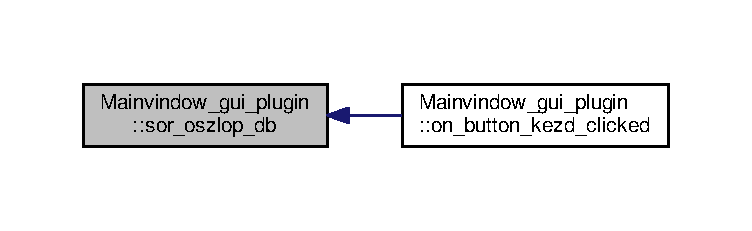
\includegraphics[width=350pt]{classMainvindow__gui__plugin_adb6c0d468163f8192f2138b15a6c43e9_icgraph}
\end{center}
\end{figure}
\mbox{\Hypertarget{classMainvindow__gui__plugin_ae7b7382ef0b52b1116426d3fc9c78caa}\label{classMainvindow__gui__plugin_ae7b7382ef0b52b1116426d3fc9c78caa}} 
\index{Mainvindow\+\_\+gui\+\_\+plugin@{Mainvindow\+\_\+gui\+\_\+plugin}!szamol@{szamol}}
\index{szamol@{szamol}!Mainvindow\+\_\+gui\+\_\+plugin@{Mainvindow\+\_\+gui\+\_\+plugin}}
\subsubsection{\texorpdfstring{szamol}{szamol}}
{\footnotesize\ttfamily void Mainvindow\+\_\+gui\+\_\+plugin\+::szamol (\begin{DoxyParamCaption}{ }\end{DoxyParamCaption})\hspace{0.3cm}{\ttfamily [signal]}}

Here is the caller graph for this function\+:\nopagebreak
\begin{figure}[H]
\begin{center}
\leavevmode
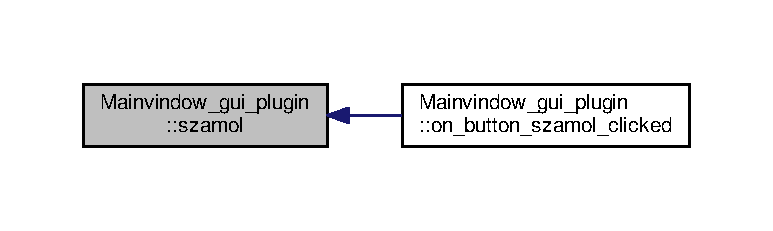
\includegraphics[width=350pt]{classMainvindow__gui__plugin_ae7b7382ef0b52b1116426d3fc9c78caa_icgraph}
\end{center}
\end{figure}
\mbox{\Hypertarget{classMainvindow__gui__plugin_a2fe7a4a60ee4e4f61579ccc717e8258d}\label{classMainvindow__gui__plugin_a2fe7a4a60ee4e4f61579ccc717e8258d}} 
\index{Mainvindow\+\_\+gui\+\_\+plugin@{Mainvindow\+\_\+gui\+\_\+plugin}!vegigszamol@{vegigszamol}}
\index{vegigszamol@{vegigszamol}!Mainvindow\+\_\+gui\+\_\+plugin@{Mainvindow\+\_\+gui\+\_\+plugin}}
\subsubsection{\texorpdfstring{vegigszamol}{vegigszamol}}
{\footnotesize\ttfamily void Mainvindow\+\_\+gui\+\_\+plugin\+::vegigszamol (\begin{DoxyParamCaption}\item[{bool}]{vegigszamolando }\end{DoxyParamCaption})\hspace{0.3cm}{\ttfamily [signal]}}

Here is the caller graph for this function\+:\nopagebreak
\begin{figure}[H]
\begin{center}
\leavevmode
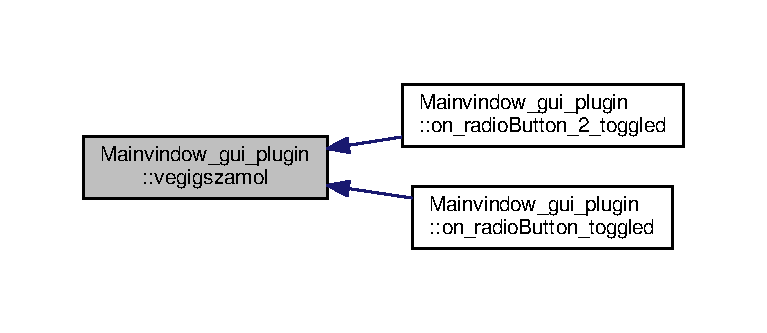
\includegraphics[width=350pt]{classMainvindow__gui__plugin_a2fe7a4a60ee4e4f61579ccc717e8258d_icgraph}
\end{center}
\end{figure}


\subsection{Member Data Documentation}
\mbox{\Hypertarget{classMainvindow__gui__plugin_adabe60e85b8b8dedc41da660506595a1}\label{classMainvindow__gui__plugin_adabe60e85b8b8dedc41da660506595a1}} 
\index{Mainvindow\+\_\+gui\+\_\+plugin@{Mainvindow\+\_\+gui\+\_\+plugin}!non\+\_\+numeric\+\_\+delegate@{non\+\_\+numeric\+\_\+delegate}}
\index{non\+\_\+numeric\+\_\+delegate@{non\+\_\+numeric\+\_\+delegate}!Mainvindow\+\_\+gui\+\_\+plugin@{Mainvindow\+\_\+gui\+\_\+plugin}}
\subsubsection{\texorpdfstring{non\+\_\+numeric\+\_\+delegate}{non\_numeric\_delegate}}
{\footnotesize\ttfamily Q\+Item\+Delegate$\ast$ Mainvindow\+\_\+gui\+\_\+plugin\+::non\+\_\+numeric\+\_\+delegate\hspace{0.3cm}{\ttfamily [private]}}



Definition at line 72 of file mainvindow\+\_\+gui\+\_\+plugin.\+h.

\mbox{\Hypertarget{classMainvindow__gui__plugin_a1ae497c20498fc8347d6d8c7691a4220}\label{classMainvindow__gui__plugin_a1ae497c20498fc8347d6d8c7691a4220}} 
\index{Mainvindow\+\_\+gui\+\_\+plugin@{Mainvindow\+\_\+gui\+\_\+plugin}!number\+\_\+delegator@{number\+\_\+delegator}}
\index{number\+\_\+delegator@{number\+\_\+delegator}!Mainvindow\+\_\+gui\+\_\+plugin@{Mainvindow\+\_\+gui\+\_\+plugin}}
\subsubsection{\texorpdfstring{number\+\_\+delegator}{number\_delegator}}
{\footnotesize\ttfamily Q\+Styled\+Item\+Delegate$\ast$ Mainvindow\+\_\+gui\+\_\+plugin\+::number\+\_\+delegator\hspace{0.3cm}{\ttfamily [private]}}



Definition at line 71 of file mainvindow\+\_\+gui\+\_\+plugin.\+h.

\mbox{\Hypertarget{classMainvindow__gui__plugin_a86399ba5cca2bb2ab811afc6dd47ccc8}\label{classMainvindow__gui__plugin_a86399ba5cca2bb2ab811afc6dd47ccc8}} 
\index{Mainvindow\+\_\+gui\+\_\+plugin@{Mainvindow\+\_\+gui\+\_\+plugin}!ui@{ui}}
\index{ui@{ui}!Mainvindow\+\_\+gui\+\_\+plugin@{Mainvindow\+\_\+gui\+\_\+plugin}}
\subsubsection{\texorpdfstring{ui}{ui}}
{\footnotesize\ttfamily Ui\+::\+Mainvindow\+\_\+gui\+\_\+plugin$\ast$ Mainvindow\+\_\+gui\+\_\+plugin\+::ui\hspace{0.3cm}{\ttfamily [private]}}



Definition at line 70 of file mainvindow\+\_\+gui\+\_\+plugin.\+h.



The documentation for this class was generated from the following files\+:\begin{DoxyCompactItemize}
\item 
Korcsolya/\hyperlink{mainvindow__gui__plugin_8h}{mainvindow\+\_\+gui\+\_\+plugin.\+h}\item 
Korcsolya/\hyperlink{mainvindow__gui__plugin_8cpp}{mainvindow\+\_\+gui\+\_\+plugin.\+cpp}\end{DoxyCompactItemize}

\hypertarget{classMainvindow__gui__plugin__for__fules}{}\section{Mainvindow\+\_\+gui\+\_\+plugin\+\_\+for\+\_\+fules Class Reference}
\label{classMainvindow__gui__plugin__for__fules}\index{Mainvindow\+\_\+gui\+\_\+plugin\+\_\+for\+\_\+fules@{Mainvindow\+\_\+gui\+\_\+plugin\+\_\+for\+\_\+fules}}


{\ttfamily \#include $<$mainvindow\+\_\+gui\+\_\+plugin\+\_\+for\+\_\+fules.\+h$>$}



Inheritance diagram for Mainvindow\+\_\+gui\+\_\+plugin\+\_\+for\+\_\+fules\+:\nopagebreak
\begin{figure}[H]
\begin{center}
\leavevmode
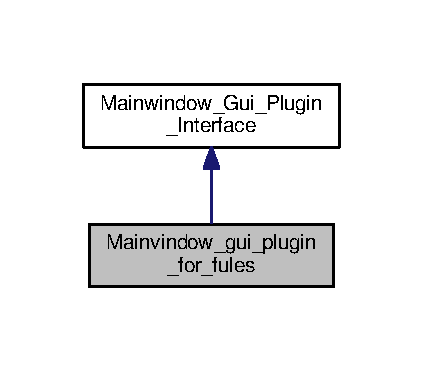
\includegraphics[width=203pt]{classMainvindow__gui__plugin__for__fules__inherit__graph}
\end{center}
\end{figure}


Collaboration diagram for Mainvindow\+\_\+gui\+\_\+plugin\+\_\+for\+\_\+fules\+:\nopagebreak
\begin{figure}[H]
\begin{center}
\leavevmode
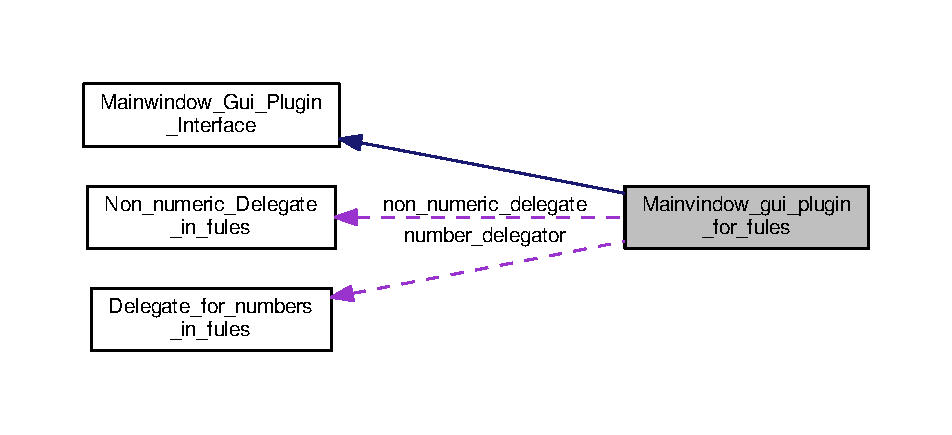
\includegraphics[width=350pt]{classMainvindow__gui__plugin__for__fules__coll__graph}
\end{center}
\end{figure}
\subsection*{Public Slots}
\begin{DoxyCompactItemize}
\item 
void \hyperlink{classMainvindow__gui__plugin__for__fules_a2429e357367c099081691f8012abdd84}{do\+\_\+set\+\_\+indulo\+\_\+model\+\_\+view} (Q\+Standard\+Item\+Model $\ast$model) Q\+\_\+\+D\+E\+C\+L\+\_\+\+O\+V\+E\+R\+R\+I\+DE
\item 
void \hyperlink{classMainvindow__gui__plugin__for__fules_af0223c6b7e5a8ab1a2c835811e61968e}{do\+\_\+set\+\_\+kanonikus\+\_\+alak\+\_\+model\+\_\+view} (Q\+Standard\+Item\+Model $\ast$model) Q\+\_\+\+D\+E\+C\+L\+\_\+\+O\+V\+E\+R\+R\+I\+DE
\item 
void \hyperlink{classMainvindow__gui__plugin__for__fules_a92ccf25dd20d9cd95bac846cee83b7f8}{do\+\_\+set\+\_\+indulo\+\_\+matrix\+\_\+model\+\_\+view} (Q\+Standard\+Item\+Model $\ast$model) Q\+\_\+\+D\+E\+C\+L\+\_\+\+O\+V\+E\+R\+R\+I\+DE
\item 
void \hyperlink{classMainvindow__gui__plugin__for__fules_a0199dc13ee862373b381eaf57716a943}{do\+\_\+set\+\_\+utolso\+\_\+elotti\+\_\+allapot\+\_\+model\+\_\+view} (Q\+Standard\+Item\+Model $\ast$model) Q\+\_\+\+D\+E\+C\+L\+\_\+\+O\+V\+E\+R\+R\+I\+DE
\item 
void \hyperlink{classMainvindow__gui__plugin__for__fules_ad441ae70c4b54bef9291ddf02d55619d}{do\+\_\+set\+\_\+utolso\+\_\+allapot\+\_\+model\+\_\+view} (Q\+Standard\+Item\+Model $\ast$model) Q\+\_\+\+D\+E\+C\+L\+\_\+\+O\+V\+E\+R\+R\+I\+DE
\item 
void \hyperlink{classMainvindow__gui__plugin__for__fules_a192a63d8fd779c87d88d8dde9626b59a}{do\+\_\+when\+\_\+indulo\+\_\+feladat\+\_\+changed} () Q\+\_\+\+D\+E\+C\+L\+\_\+\+O\+V\+E\+R\+R\+I\+DE
\item 
void \hyperlink{classMainvindow__gui__plugin__for__fules_aaab6c53ad37973164d334745ab2fbec5}{do\+\_\+when\+\_\+vegigszamol\+\_\+changed} (bool checked) Q\+\_\+\+D\+E\+C\+L\+\_\+\+O\+V\+E\+R\+R\+I\+DE
\item 
void \hyperlink{classMainvindow__gui__plugin__for__fules_a32904586a5f9f8512fb9d3bdd8b92f4b}{do\+\_\+when\+\_\+external\+\_\+exercise\+\_\+loaded} (int termtenyezo, int korl\+\_\+felt) Q\+\_\+\+D\+E\+C\+L\+\_\+\+O\+V\+E\+R\+R\+I\+DE
\item 
void \hyperlink{classMainvindow__gui__plugin__for__fules_ab18bc74a0030c8cc05853074589c1b77}{do\+\_\+when\+\_\+got\+\_\+kanonikus\+\_\+clicked} () Q\+\_\+\+D\+E\+C\+L\+\_\+\+O\+V\+E\+R\+R\+I\+DE
\item 
void \hyperlink{classMainvindow__gui__plugin__for__fules_a79f10558ac2aaba9cee238b3fde817ae}{do\+\_\+when\+\_\+got\+\_\+indulo\+\_\+matrix\+\_\+clicked} () Q\+\_\+\+D\+E\+C\+L\+\_\+\+O\+V\+E\+R\+R\+I\+DE
\item 
void \hyperlink{classMainvindow__gui__plugin__for__fules_a7a76e31c7008ec8a41db6dc0ebbe20ee}{do\+\_\+set\+\_\+delegate\+\_\+for\+\_\+numbers} (Q\+Styled\+Item\+Delegate $\ast$delegate) Q\+\_\+\+D\+E\+C\+L\+\_\+\+O\+V\+E\+R\+R\+I\+DE
\begin{DoxyCompactList}\small\item\em A fő program altal biztosított numerikus delegátor beállítása. \end{DoxyCompactList}\item 
void \hyperlink{classMainvindow__gui__plugin__for__fules_a260b143aa4bf25e3f8fa6d2de08aca3d}{do\+\_\+set\+\_\+non\+\_\+numeric\+\_\+delegate} (Q\+Item\+Delegate $\ast$delegate) Q\+\_\+\+D\+E\+C\+L\+\_\+\+O\+V\+E\+R\+R\+I\+DE
\begin{DoxyCompactList}\small\item\em A fő program altal biztosított nem-\/numerikus delegátor beállítása. \end{DoxyCompactList}\item 
void \hyperlink{classMainvindow__gui__plugin__for__fules_ab655a7eceb4371004b43ae4e29cc4244}{do\+\_\+when\+\_\+button\+\_\+kezd\+\_\+clicked} (int termteny, int korlfelt) Q\+\_\+\+D\+E\+C\+L\+\_\+\+O\+V\+E\+R\+R\+I\+DE
\end{DoxyCompactItemize}
\subsection*{Signals}
\begin{DoxyCompactItemize}
\item 
void \hyperlink{classMainvindow__gui__plugin__for__fules_a04e1668bac22f62c014954222d19f2ac}{sor\+\_\+oszlop\+\_\+db} (int, int) Q\+\_\+\+D\+E\+C\+L\+\_\+\+F\+I\+N\+AL
\item 
void \hyperlink{classMainvindow__gui__plugin__for__fules_ad57320bcd6e0f8353254601919b980b9}{make\+\_\+kanonikus} () Q\+\_\+\+D\+E\+C\+L\+\_\+\+F\+I\+N\+AL
\item 
void \hyperlink{classMainvindow__gui__plugin__for__fules_a69be0da66c49005cb7178c140b53dccb}{make\+\_\+indulo\+\_\+matrix} () Q\+\_\+\+D\+E\+C\+L\+\_\+\+F\+I\+N\+AL
\item 
void \hyperlink{classMainvindow__gui__plugin__for__fules_ab44bcc45064b346477fef5df26a119cc}{szamol} () Q\+\_\+\+D\+E\+C\+L\+\_\+\+F\+I\+N\+AL
\item 
void \hyperlink{classMainvindow__gui__plugin__for__fules_a080c54bd4e8e65ffcaacad58e900248a}{vegigszamol} (bool vegigszamolando) Q\+\_\+\+D\+E\+C\+L\+\_\+\+F\+I\+N\+AL
\item 
void \hyperlink{classMainvindow__gui__plugin__for__fules_a4ca08e417e9b4784db455ed9016870cc}{kanonikus\+\_\+clicked} () Q\+\_\+\+D\+E\+C\+L\+\_\+\+F\+I\+N\+AL
\item 
void \hyperlink{classMainvindow__gui__plugin__for__fules_a1b7701944f9234161efae2663b5c660f}{indulo\+\_\+matrix\+\_\+clicked} () Q\+\_\+\+D\+E\+C\+L\+\_\+\+F\+I\+N\+AL
\end{DoxyCompactItemize}
\subsection*{Public Member Functions}
\begin{DoxyCompactItemize}
\item 
\hyperlink{classMainvindow__gui__plugin__for__fules_aeb68fbca198b45e19deee3af31e550e5}{Mainvindow\+\_\+gui\+\_\+plugin\+\_\+for\+\_\+fules} (Q\+Widget $\ast$parent=nullptr)
\item 
\hyperlink{classMainvindow__gui__plugin__for__fules_a202c933c2c305081247fb1c334e1a020}{$\sim$\+Mainvindow\+\_\+gui\+\_\+plugin\+\_\+for\+\_\+fules} () override
\item 
Q\+String \hyperlink{classMainvindow__gui__plugin__for__fules_abfd45e12e05f78b189c4ad00f7fb6930}{Name} () const override
\end{DoxyCompactItemize}
\subsection*{Private Slots}
\begin{DoxyCompactItemize}
\item 
void \hyperlink{classMainvindow__gui__plugin__for__fules_ae30db934e0e08f96cebd31c051fc43c5}{on\+\_\+button\+\_\+szamol\+\_\+clicked} ()
\item 
void \hyperlink{classMainvindow__gui__plugin__for__fules_aea9911335d30ac911adf04aa5ccfd8ee}{on\+\_\+button\+\_\+indulo\+\_\+matrix\+\_\+clicked} ()
\item 
void \hyperlink{classMainvindow__gui__plugin__for__fules_ae833c3ac5845928744df35c255c80a76}{on\+\_\+button\+\_\+kezd\+\_\+clicked} ()
\item 
void \hyperlink{classMainvindow__gui__plugin__for__fules_adc6ad081195bda78f2d2c93736aba030}{on\+\_\+button\+\_\+kanonikus\+\_\+clicked} ()
\item 
void \hyperlink{classMainvindow__gui__plugin__for__fules_a40fb3f212d108731599d9a3e106ad65b}{on\+\_\+radio\+Button\+\_\+2\+\_\+toggled} (bool checked)
\item 
void \hyperlink{classMainvindow__gui__plugin__for__fules_a8c33c824b142bea8995e3dd12f081f21}{on\+\_\+radio\+Button\+\_\+toggled} (bool checked)
\end{DoxyCompactItemize}
\subsection*{Private Attributes}
\begin{DoxyCompactItemize}
\item 
Ui\+::\+Mainvindow\+\_\+gui\+\_\+plugin\+\_\+for\+\_\+fules $\ast$ \hyperlink{classMainvindow__gui__plugin__for__fules_acdd8ed5ce96f1565bc722f1965faca67}{ui}
\item 
\hyperlink{classDelegate__for__numbers__in__fules}{Delegate\+\_\+for\+\_\+numbers\+\_\+in\+\_\+fules} $\ast$ \hyperlink{classMainvindow__gui__plugin__for__fules_a6b1f4a0fae34535113840411223ccfa6}{number\+\_\+delegator}
\item 
\hyperlink{classNon__numeric__Delegate__in__fules}{Non\+\_\+numeric\+\_\+\+Delegate\+\_\+in\+\_\+fules} $\ast$ \hyperlink{classMainvindow__gui__plugin__for__fules_aea0a3b7f00e651f970723dab3338240d}{non\+\_\+numeric\+\_\+delegate}
\end{DoxyCompactItemize}


\subsection{Detailed Description}


Definition at line 13 of file mainvindow\+\_\+gui\+\_\+plugin\+\_\+for\+\_\+fules.\+h.



\subsection{Constructor \& Destructor Documentation}
\mbox{\Hypertarget{classMainvindow__gui__plugin__for__fules_aeb68fbca198b45e19deee3af31e550e5}\label{classMainvindow__gui__plugin__for__fules_aeb68fbca198b45e19deee3af31e550e5}} 
\index{Mainvindow\+\_\+gui\+\_\+plugin\+\_\+for\+\_\+fules@{Mainvindow\+\_\+gui\+\_\+plugin\+\_\+for\+\_\+fules}!Mainvindow\+\_\+gui\+\_\+plugin\+\_\+for\+\_\+fules@{Mainvindow\+\_\+gui\+\_\+plugin\+\_\+for\+\_\+fules}}
\index{Mainvindow\+\_\+gui\+\_\+plugin\+\_\+for\+\_\+fules@{Mainvindow\+\_\+gui\+\_\+plugin\+\_\+for\+\_\+fules}!Mainvindow\+\_\+gui\+\_\+plugin\+\_\+for\+\_\+fules@{Mainvindow\+\_\+gui\+\_\+plugin\+\_\+for\+\_\+fules}}
\subsubsection{\texorpdfstring{Mainvindow\+\_\+gui\+\_\+plugin\+\_\+for\+\_\+fules()}{Mainvindow\_gui\_plugin\_for\_fules()}}
{\footnotesize\ttfamily Mainvindow\+\_\+gui\+\_\+plugin\+\_\+for\+\_\+fules\+::\+Mainvindow\+\_\+gui\+\_\+plugin\+\_\+for\+\_\+fules (\begin{DoxyParamCaption}\item[{Q\+Widget $\ast$}]{parent = {\ttfamily nullptr} }\end{DoxyParamCaption})\hspace{0.3cm}{\ttfamily [explicit]}}



Definition at line 4 of file mainvindow\+\_\+gui\+\_\+plugin\+\_\+for\+\_\+fules.\+cpp.

\mbox{\Hypertarget{classMainvindow__gui__plugin__for__fules_a202c933c2c305081247fb1c334e1a020}\label{classMainvindow__gui__plugin__for__fules_a202c933c2c305081247fb1c334e1a020}} 
\index{Mainvindow\+\_\+gui\+\_\+plugin\+\_\+for\+\_\+fules@{Mainvindow\+\_\+gui\+\_\+plugin\+\_\+for\+\_\+fules}!````~Mainvindow\+\_\+gui\+\_\+plugin\+\_\+for\+\_\+fules@{$\sim$\+Mainvindow\+\_\+gui\+\_\+plugin\+\_\+for\+\_\+fules}}
\index{````~Mainvindow\+\_\+gui\+\_\+plugin\+\_\+for\+\_\+fules@{$\sim$\+Mainvindow\+\_\+gui\+\_\+plugin\+\_\+for\+\_\+fules}!Mainvindow\+\_\+gui\+\_\+plugin\+\_\+for\+\_\+fules@{Mainvindow\+\_\+gui\+\_\+plugin\+\_\+for\+\_\+fules}}
\subsubsection{\texorpdfstring{$\sim$\+Mainvindow\+\_\+gui\+\_\+plugin\+\_\+for\+\_\+fules()}{~Mainvindow\_gui\_plugin\_for\_fules()}}
{\footnotesize\ttfamily Mainvindow\+\_\+gui\+\_\+plugin\+\_\+for\+\_\+fules\+::$\sim$\+Mainvindow\+\_\+gui\+\_\+plugin\+\_\+for\+\_\+fules (\begin{DoxyParamCaption}{ }\end{DoxyParamCaption})\hspace{0.3cm}{\ttfamily [override]}}



Definition at line 20 of file mainvindow\+\_\+gui\+\_\+plugin\+\_\+for\+\_\+fules.\+cpp.



\subsection{Member Function Documentation}
\mbox{\Hypertarget{classMainvindow__gui__plugin__for__fules_a7a76e31c7008ec8a41db6dc0ebbe20ee}\label{classMainvindow__gui__plugin__for__fules_a7a76e31c7008ec8a41db6dc0ebbe20ee}} 
\index{Mainvindow\+\_\+gui\+\_\+plugin\+\_\+for\+\_\+fules@{Mainvindow\+\_\+gui\+\_\+plugin\+\_\+for\+\_\+fules}!do\+\_\+set\+\_\+delegate\+\_\+for\+\_\+numbers@{do\+\_\+set\+\_\+delegate\+\_\+for\+\_\+numbers}}
\index{do\+\_\+set\+\_\+delegate\+\_\+for\+\_\+numbers@{do\+\_\+set\+\_\+delegate\+\_\+for\+\_\+numbers}!Mainvindow\+\_\+gui\+\_\+plugin\+\_\+for\+\_\+fules@{Mainvindow\+\_\+gui\+\_\+plugin\+\_\+for\+\_\+fules}}
\subsubsection{\texorpdfstring{do\+\_\+set\+\_\+delegate\+\_\+for\+\_\+numbers}{do\_set\_delegate\_for\_numbers}}
{\footnotesize\ttfamily void Mainvindow\+\_\+gui\+\_\+plugin\+\_\+for\+\_\+fules\+::do\+\_\+set\+\_\+delegate\+\_\+for\+\_\+numbers (\begin{DoxyParamCaption}\item[{Q\+Styled\+Item\+Delegate $\ast$}]{delegate }\end{DoxyParamCaption})\hspace{0.3cm}{\ttfamily [slot]}}



A fő program altal biztosított numerikus delegátor beállítása. 

A fő program biztosít agy alap delegátort a numerikus adatoknak. Itt azonban -\/mivel ez az osztály saját delegátorát hazsnálja-\/ üres.


\begin{DoxyParams}{Parameters}
{\em delegate} & A főprogram által biztosított numerikus delegátorra mutató pointer. \\
\hline
\end{DoxyParams}


Definition at line 178 of file mainvindow\+\_\+gui\+\_\+plugin\+\_\+for\+\_\+fules.\+cpp.

\mbox{\Hypertarget{classMainvindow__gui__plugin__for__fules_a92ccf25dd20d9cd95bac846cee83b7f8}\label{classMainvindow__gui__plugin__for__fules_a92ccf25dd20d9cd95bac846cee83b7f8}} 
\index{Mainvindow\+\_\+gui\+\_\+plugin\+\_\+for\+\_\+fules@{Mainvindow\+\_\+gui\+\_\+plugin\+\_\+for\+\_\+fules}!do\+\_\+set\+\_\+indulo\+\_\+matrix\+\_\+model\+\_\+view@{do\+\_\+set\+\_\+indulo\+\_\+matrix\+\_\+model\+\_\+view}}
\index{do\+\_\+set\+\_\+indulo\+\_\+matrix\+\_\+model\+\_\+view@{do\+\_\+set\+\_\+indulo\+\_\+matrix\+\_\+model\+\_\+view}!Mainvindow\+\_\+gui\+\_\+plugin\+\_\+for\+\_\+fules@{Mainvindow\+\_\+gui\+\_\+plugin\+\_\+for\+\_\+fules}}
\subsubsection{\texorpdfstring{do\+\_\+set\+\_\+indulo\+\_\+matrix\+\_\+model\+\_\+view}{do\_set\_indulo\_matrix\_model\_view}}
{\footnotesize\ttfamily void Mainvindow\+\_\+gui\+\_\+plugin\+\_\+for\+\_\+fules\+::do\+\_\+set\+\_\+indulo\+\_\+matrix\+\_\+model\+\_\+view (\begin{DoxyParamCaption}\item[{Q\+Standard\+Item\+Model $\ast$}]{model }\end{DoxyParamCaption})\hspace{0.3cm}{\ttfamily [slot]}}



Definition at line 35 of file mainvindow\+\_\+gui\+\_\+plugin\+\_\+for\+\_\+fules.\+cpp.

\mbox{\Hypertarget{classMainvindow__gui__plugin__for__fules_a2429e357367c099081691f8012abdd84}\label{classMainvindow__gui__plugin__for__fules_a2429e357367c099081691f8012abdd84}} 
\index{Mainvindow\+\_\+gui\+\_\+plugin\+\_\+for\+\_\+fules@{Mainvindow\+\_\+gui\+\_\+plugin\+\_\+for\+\_\+fules}!do\+\_\+set\+\_\+indulo\+\_\+model\+\_\+view@{do\+\_\+set\+\_\+indulo\+\_\+model\+\_\+view}}
\index{do\+\_\+set\+\_\+indulo\+\_\+model\+\_\+view@{do\+\_\+set\+\_\+indulo\+\_\+model\+\_\+view}!Mainvindow\+\_\+gui\+\_\+plugin\+\_\+for\+\_\+fules@{Mainvindow\+\_\+gui\+\_\+plugin\+\_\+for\+\_\+fules}}
\subsubsection{\texorpdfstring{do\+\_\+set\+\_\+indulo\+\_\+model\+\_\+view}{do\_set\_indulo\_model\_view}}
{\footnotesize\ttfamily void Mainvindow\+\_\+gui\+\_\+plugin\+\_\+for\+\_\+fules\+::do\+\_\+set\+\_\+indulo\+\_\+model\+\_\+view (\begin{DoxyParamCaption}\item[{Q\+Standard\+Item\+Model $\ast$}]{model }\end{DoxyParamCaption})\hspace{0.3cm}{\ttfamily [slot]}}



Definition at line 24 of file mainvindow\+\_\+gui\+\_\+plugin\+\_\+for\+\_\+fules.\+cpp.

\mbox{\Hypertarget{classMainvindow__gui__plugin__for__fules_af0223c6b7e5a8ab1a2c835811e61968e}\label{classMainvindow__gui__plugin__for__fules_af0223c6b7e5a8ab1a2c835811e61968e}} 
\index{Mainvindow\+\_\+gui\+\_\+plugin\+\_\+for\+\_\+fules@{Mainvindow\+\_\+gui\+\_\+plugin\+\_\+for\+\_\+fules}!do\+\_\+set\+\_\+kanonikus\+\_\+alak\+\_\+model\+\_\+view@{do\+\_\+set\+\_\+kanonikus\+\_\+alak\+\_\+model\+\_\+view}}
\index{do\+\_\+set\+\_\+kanonikus\+\_\+alak\+\_\+model\+\_\+view@{do\+\_\+set\+\_\+kanonikus\+\_\+alak\+\_\+model\+\_\+view}!Mainvindow\+\_\+gui\+\_\+plugin\+\_\+for\+\_\+fules@{Mainvindow\+\_\+gui\+\_\+plugin\+\_\+for\+\_\+fules}}
\subsubsection{\texorpdfstring{do\+\_\+set\+\_\+kanonikus\+\_\+alak\+\_\+model\+\_\+view}{do\_set\_kanonikus\_alak\_model\_view}}
{\footnotesize\ttfamily void Mainvindow\+\_\+gui\+\_\+plugin\+\_\+for\+\_\+fules\+::do\+\_\+set\+\_\+kanonikus\+\_\+alak\+\_\+model\+\_\+view (\begin{DoxyParamCaption}\item[{Q\+Standard\+Item\+Model $\ast$}]{model }\end{DoxyParamCaption})\hspace{0.3cm}{\ttfamily [slot]}}



Definition at line 31 of file mainvindow\+\_\+gui\+\_\+plugin\+\_\+for\+\_\+fules.\+cpp.

\mbox{\Hypertarget{classMainvindow__gui__plugin__for__fules_a260b143aa4bf25e3f8fa6d2de08aca3d}\label{classMainvindow__gui__plugin__for__fules_a260b143aa4bf25e3f8fa6d2de08aca3d}} 
\index{Mainvindow\+\_\+gui\+\_\+plugin\+\_\+for\+\_\+fules@{Mainvindow\+\_\+gui\+\_\+plugin\+\_\+for\+\_\+fules}!do\+\_\+set\+\_\+non\+\_\+numeric\+\_\+delegate@{do\+\_\+set\+\_\+non\+\_\+numeric\+\_\+delegate}}
\index{do\+\_\+set\+\_\+non\+\_\+numeric\+\_\+delegate@{do\+\_\+set\+\_\+non\+\_\+numeric\+\_\+delegate}!Mainvindow\+\_\+gui\+\_\+plugin\+\_\+for\+\_\+fules@{Mainvindow\+\_\+gui\+\_\+plugin\+\_\+for\+\_\+fules}}
\subsubsection{\texorpdfstring{do\+\_\+set\+\_\+non\+\_\+numeric\+\_\+delegate}{do\_set\_non\_numeric\_delegate}}
{\footnotesize\ttfamily void Mainvindow\+\_\+gui\+\_\+plugin\+\_\+for\+\_\+fules\+::do\+\_\+set\+\_\+non\+\_\+numeric\+\_\+delegate (\begin{DoxyParamCaption}\item[{Q\+Item\+Delegate $\ast$}]{delegate }\end{DoxyParamCaption})\hspace{0.3cm}{\ttfamily [slot]}}



A fő program altal biztosított nem-\/numerikus delegátor beállítása. 

A fő program biztosít agy alap delegátort a nem-\/numerikus adatoknak. Itt azonban -\/mivel ez az osztály saját delegátorát hazsnálja-\/ üres.


\begin{DoxyParams}{Parameters}
{\em delegate} & A főprogram által biztosított nem-\/numerikus delegátorra mutató pointer. \\
\hline
\end{DoxyParams}


Definition at line 193 of file mainvindow\+\_\+gui\+\_\+plugin\+\_\+for\+\_\+fules.\+cpp.

\mbox{\Hypertarget{classMainvindow__gui__plugin__for__fules_ad441ae70c4b54bef9291ddf02d55619d}\label{classMainvindow__gui__plugin__for__fules_ad441ae70c4b54bef9291ddf02d55619d}} 
\index{Mainvindow\+\_\+gui\+\_\+plugin\+\_\+for\+\_\+fules@{Mainvindow\+\_\+gui\+\_\+plugin\+\_\+for\+\_\+fules}!do\+\_\+set\+\_\+utolso\+\_\+allapot\+\_\+model\+\_\+view@{do\+\_\+set\+\_\+utolso\+\_\+allapot\+\_\+model\+\_\+view}}
\index{do\+\_\+set\+\_\+utolso\+\_\+allapot\+\_\+model\+\_\+view@{do\+\_\+set\+\_\+utolso\+\_\+allapot\+\_\+model\+\_\+view}!Mainvindow\+\_\+gui\+\_\+plugin\+\_\+for\+\_\+fules@{Mainvindow\+\_\+gui\+\_\+plugin\+\_\+for\+\_\+fules}}
\subsubsection{\texorpdfstring{do\+\_\+set\+\_\+utolso\+\_\+allapot\+\_\+model\+\_\+view}{do\_set\_utolso\_allapot\_model\_view}}
{\footnotesize\ttfamily void Mainvindow\+\_\+gui\+\_\+plugin\+\_\+for\+\_\+fules\+::do\+\_\+set\+\_\+utolso\+\_\+allapot\+\_\+model\+\_\+view (\begin{DoxyParamCaption}\item[{Q\+Standard\+Item\+Model $\ast$}]{model }\end{DoxyParamCaption})\hspace{0.3cm}{\ttfamily [slot]}}



Definition at line 49 of file mainvindow\+\_\+gui\+\_\+plugin\+\_\+for\+\_\+fules.\+cpp.

\mbox{\Hypertarget{classMainvindow__gui__plugin__for__fules_a0199dc13ee862373b381eaf57716a943}\label{classMainvindow__gui__plugin__for__fules_a0199dc13ee862373b381eaf57716a943}} 
\index{Mainvindow\+\_\+gui\+\_\+plugin\+\_\+for\+\_\+fules@{Mainvindow\+\_\+gui\+\_\+plugin\+\_\+for\+\_\+fules}!do\+\_\+set\+\_\+utolso\+\_\+elotti\+\_\+allapot\+\_\+model\+\_\+view@{do\+\_\+set\+\_\+utolso\+\_\+elotti\+\_\+allapot\+\_\+model\+\_\+view}}
\index{do\+\_\+set\+\_\+utolso\+\_\+elotti\+\_\+allapot\+\_\+model\+\_\+view@{do\+\_\+set\+\_\+utolso\+\_\+elotti\+\_\+allapot\+\_\+model\+\_\+view}!Mainvindow\+\_\+gui\+\_\+plugin\+\_\+for\+\_\+fules@{Mainvindow\+\_\+gui\+\_\+plugin\+\_\+for\+\_\+fules}}
\subsubsection{\texorpdfstring{do\+\_\+set\+\_\+utolso\+\_\+elotti\+\_\+allapot\+\_\+model\+\_\+view}{do\_set\_utolso\_elotti\_allapot\_model\_view}}
{\footnotesize\ttfamily void Mainvindow\+\_\+gui\+\_\+plugin\+\_\+for\+\_\+fules\+::do\+\_\+set\+\_\+utolso\+\_\+elotti\+\_\+allapot\+\_\+model\+\_\+view (\begin{DoxyParamCaption}\item[{Q\+Standard\+Item\+Model $\ast$}]{model }\end{DoxyParamCaption})\hspace{0.3cm}{\ttfamily [slot]}}



Definition at line 42 of file mainvindow\+\_\+gui\+\_\+plugin\+\_\+for\+\_\+fules.\+cpp.

\mbox{\Hypertarget{classMainvindow__gui__plugin__for__fules_ab655a7eceb4371004b43ae4e29cc4244}\label{classMainvindow__gui__plugin__for__fules_ab655a7eceb4371004b43ae4e29cc4244}} 
\index{Mainvindow\+\_\+gui\+\_\+plugin\+\_\+for\+\_\+fules@{Mainvindow\+\_\+gui\+\_\+plugin\+\_\+for\+\_\+fules}!do\+\_\+when\+\_\+button\+\_\+kezd\+\_\+clicked@{do\+\_\+when\+\_\+button\+\_\+kezd\+\_\+clicked}}
\index{do\+\_\+when\+\_\+button\+\_\+kezd\+\_\+clicked@{do\+\_\+when\+\_\+button\+\_\+kezd\+\_\+clicked}!Mainvindow\+\_\+gui\+\_\+plugin\+\_\+for\+\_\+fules@{Mainvindow\+\_\+gui\+\_\+plugin\+\_\+for\+\_\+fules}}
\subsubsection{\texorpdfstring{do\+\_\+when\+\_\+button\+\_\+kezd\+\_\+clicked}{do\_when\_button\_kezd\_clicked}}
{\footnotesize\ttfamily void Mainvindow\+\_\+gui\+\_\+plugin\+\_\+for\+\_\+fules\+::do\+\_\+when\+\_\+button\+\_\+kezd\+\_\+clicked (\begin{DoxyParamCaption}\item[{int}]{termteny,  }\item[{int}]{korlfelt }\end{DoxyParamCaption})\hspace{0.3cm}{\ttfamily [slot]}}



Definition at line 91 of file mainvindow\+\_\+gui\+\_\+plugin\+\_\+for\+\_\+fules.\+cpp.

\mbox{\Hypertarget{classMainvindow__gui__plugin__for__fules_a32904586a5f9f8512fb9d3bdd8b92f4b}\label{classMainvindow__gui__plugin__for__fules_a32904586a5f9f8512fb9d3bdd8b92f4b}} 
\index{Mainvindow\+\_\+gui\+\_\+plugin\+\_\+for\+\_\+fules@{Mainvindow\+\_\+gui\+\_\+plugin\+\_\+for\+\_\+fules}!do\+\_\+when\+\_\+external\+\_\+exercise\+\_\+loaded@{do\+\_\+when\+\_\+external\+\_\+exercise\+\_\+loaded}}
\index{do\+\_\+when\+\_\+external\+\_\+exercise\+\_\+loaded@{do\+\_\+when\+\_\+external\+\_\+exercise\+\_\+loaded}!Mainvindow\+\_\+gui\+\_\+plugin\+\_\+for\+\_\+fules@{Mainvindow\+\_\+gui\+\_\+plugin\+\_\+for\+\_\+fules}}
\subsubsection{\texorpdfstring{do\+\_\+when\+\_\+external\+\_\+exercise\+\_\+loaded}{do\_when\_external\_exercise\_loaded}}
{\footnotesize\ttfamily void Mainvindow\+\_\+gui\+\_\+plugin\+\_\+for\+\_\+fules\+::do\+\_\+when\+\_\+external\+\_\+exercise\+\_\+loaded (\begin{DoxyParamCaption}\item[{int}]{termtenyezo,  }\item[{int}]{korl\+\_\+felt }\end{DoxyParamCaption})\hspace{0.3cm}{\ttfamily [slot]}}



Definition at line 152 of file mainvindow\+\_\+gui\+\_\+plugin\+\_\+for\+\_\+fules.\+cpp.

\mbox{\Hypertarget{classMainvindow__gui__plugin__for__fules_a79f10558ac2aaba9cee238b3fde817ae}\label{classMainvindow__gui__plugin__for__fules_a79f10558ac2aaba9cee238b3fde817ae}} 
\index{Mainvindow\+\_\+gui\+\_\+plugin\+\_\+for\+\_\+fules@{Mainvindow\+\_\+gui\+\_\+plugin\+\_\+for\+\_\+fules}!do\+\_\+when\+\_\+got\+\_\+indulo\+\_\+matrix\+\_\+clicked@{do\+\_\+when\+\_\+got\+\_\+indulo\+\_\+matrix\+\_\+clicked}}
\index{do\+\_\+when\+\_\+got\+\_\+indulo\+\_\+matrix\+\_\+clicked@{do\+\_\+when\+\_\+got\+\_\+indulo\+\_\+matrix\+\_\+clicked}!Mainvindow\+\_\+gui\+\_\+plugin\+\_\+for\+\_\+fules@{Mainvindow\+\_\+gui\+\_\+plugin\+\_\+for\+\_\+fules}}
\subsubsection{\texorpdfstring{do\+\_\+when\+\_\+got\+\_\+indulo\+\_\+matrix\+\_\+clicked}{do\_when\_got\_indulo\_matrix\_clicked}}
{\footnotesize\ttfamily void Mainvindow\+\_\+gui\+\_\+plugin\+\_\+for\+\_\+fules\+::do\+\_\+when\+\_\+got\+\_\+indulo\+\_\+matrix\+\_\+clicked (\begin{DoxyParamCaption}{ }\end{DoxyParamCaption})\hspace{0.3cm}{\ttfamily [slot]}}



Definition at line 77 of file mainvindow\+\_\+gui\+\_\+plugin\+\_\+for\+\_\+fules.\+cpp.

\mbox{\Hypertarget{classMainvindow__gui__plugin__for__fules_ab18bc74a0030c8cc05853074589c1b77}\label{classMainvindow__gui__plugin__for__fules_ab18bc74a0030c8cc05853074589c1b77}} 
\index{Mainvindow\+\_\+gui\+\_\+plugin\+\_\+for\+\_\+fules@{Mainvindow\+\_\+gui\+\_\+plugin\+\_\+for\+\_\+fules}!do\+\_\+when\+\_\+got\+\_\+kanonikus\+\_\+clicked@{do\+\_\+when\+\_\+got\+\_\+kanonikus\+\_\+clicked}}
\index{do\+\_\+when\+\_\+got\+\_\+kanonikus\+\_\+clicked@{do\+\_\+when\+\_\+got\+\_\+kanonikus\+\_\+clicked}!Mainvindow\+\_\+gui\+\_\+plugin\+\_\+for\+\_\+fules@{Mainvindow\+\_\+gui\+\_\+plugin\+\_\+for\+\_\+fules}}
\subsubsection{\texorpdfstring{do\+\_\+when\+\_\+got\+\_\+kanonikus\+\_\+clicked}{do\_when\_got\_kanonikus\_clicked}}
{\footnotesize\ttfamily void Mainvindow\+\_\+gui\+\_\+plugin\+\_\+for\+\_\+fules\+::do\+\_\+when\+\_\+got\+\_\+kanonikus\+\_\+clicked (\begin{DoxyParamCaption}{ }\end{DoxyParamCaption})\hspace{0.3cm}{\ttfamily [slot]}}



Definition at line 115 of file mainvindow\+\_\+gui\+\_\+plugin\+\_\+for\+\_\+fules.\+cpp.

\mbox{\Hypertarget{classMainvindow__gui__plugin__for__fules_a192a63d8fd779c87d88d8dde9626b59a}\label{classMainvindow__gui__plugin__for__fules_a192a63d8fd779c87d88d8dde9626b59a}} 
\index{Mainvindow\+\_\+gui\+\_\+plugin\+\_\+for\+\_\+fules@{Mainvindow\+\_\+gui\+\_\+plugin\+\_\+for\+\_\+fules}!do\+\_\+when\+\_\+indulo\+\_\+feladat\+\_\+changed@{do\+\_\+when\+\_\+indulo\+\_\+feladat\+\_\+changed}}
\index{do\+\_\+when\+\_\+indulo\+\_\+feladat\+\_\+changed@{do\+\_\+when\+\_\+indulo\+\_\+feladat\+\_\+changed}!Mainvindow\+\_\+gui\+\_\+plugin\+\_\+for\+\_\+fules@{Mainvindow\+\_\+gui\+\_\+plugin\+\_\+for\+\_\+fules}}
\subsubsection{\texorpdfstring{do\+\_\+when\+\_\+indulo\+\_\+feladat\+\_\+changed}{do\_when\_indulo\_feladat\_changed}}
{\footnotesize\ttfamily void Mainvindow\+\_\+gui\+\_\+plugin\+\_\+for\+\_\+fules\+::do\+\_\+when\+\_\+indulo\+\_\+feladat\+\_\+changed (\begin{DoxyParamCaption}{ }\end{DoxyParamCaption})\hspace{0.3cm}{\ttfamily [slot]}}



Definition at line 125 of file mainvindow\+\_\+gui\+\_\+plugin\+\_\+for\+\_\+fules.\+cpp.

\mbox{\Hypertarget{classMainvindow__gui__plugin__for__fules_aaab6c53ad37973164d334745ab2fbec5}\label{classMainvindow__gui__plugin__for__fules_aaab6c53ad37973164d334745ab2fbec5}} 
\index{Mainvindow\+\_\+gui\+\_\+plugin\+\_\+for\+\_\+fules@{Mainvindow\+\_\+gui\+\_\+plugin\+\_\+for\+\_\+fules}!do\+\_\+when\+\_\+vegigszamol\+\_\+changed@{do\+\_\+when\+\_\+vegigszamol\+\_\+changed}}
\index{do\+\_\+when\+\_\+vegigszamol\+\_\+changed@{do\+\_\+when\+\_\+vegigszamol\+\_\+changed}!Mainvindow\+\_\+gui\+\_\+plugin\+\_\+for\+\_\+fules@{Mainvindow\+\_\+gui\+\_\+plugin\+\_\+for\+\_\+fules}}
\subsubsection{\texorpdfstring{do\+\_\+when\+\_\+vegigszamol\+\_\+changed}{do\_when\_vegigszamol\_changed}}
{\footnotesize\ttfamily void Mainvindow\+\_\+gui\+\_\+plugin\+\_\+for\+\_\+fules\+::do\+\_\+when\+\_\+vegigszamol\+\_\+changed (\begin{DoxyParamCaption}\item[{bool}]{checked }\end{DoxyParamCaption})\hspace{0.3cm}{\ttfamily [slot]}}



Definition at line 141 of file mainvindow\+\_\+gui\+\_\+plugin\+\_\+for\+\_\+fules.\+cpp.

\mbox{\Hypertarget{classMainvindow__gui__plugin__for__fules_a1b7701944f9234161efae2663b5c660f}\label{classMainvindow__gui__plugin__for__fules_a1b7701944f9234161efae2663b5c660f}} 
\index{Mainvindow\+\_\+gui\+\_\+plugin\+\_\+for\+\_\+fules@{Mainvindow\+\_\+gui\+\_\+plugin\+\_\+for\+\_\+fules}!indulo\+\_\+matrix\+\_\+clicked@{indulo\+\_\+matrix\+\_\+clicked}}
\index{indulo\+\_\+matrix\+\_\+clicked@{indulo\+\_\+matrix\+\_\+clicked}!Mainvindow\+\_\+gui\+\_\+plugin\+\_\+for\+\_\+fules@{Mainvindow\+\_\+gui\+\_\+plugin\+\_\+for\+\_\+fules}}
\subsubsection{\texorpdfstring{indulo\+\_\+matrix\+\_\+clicked}{indulo\_matrix\_clicked}}
{\footnotesize\ttfamily void Mainvindow\+\_\+gui\+\_\+plugin\+\_\+for\+\_\+fules\+::indulo\+\_\+matrix\+\_\+clicked (\begin{DoxyParamCaption}{ }\end{DoxyParamCaption})\hspace{0.3cm}{\ttfamily [signal]}}

Here is the caller graph for this function\+:\nopagebreak
\begin{figure}[H]
\begin{center}
\leavevmode
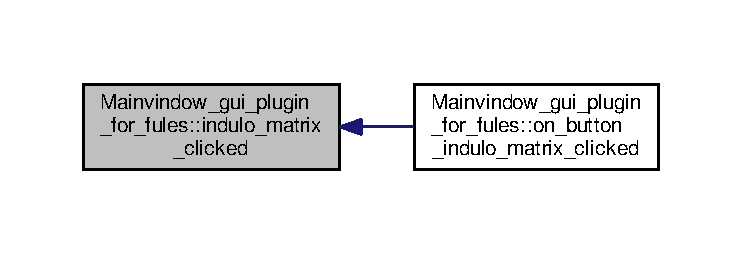
\includegraphics[width=350pt]{classMainvindow__gui__plugin__for__fules_a1b7701944f9234161efae2663b5c660f_icgraph}
\end{center}
\end{figure}
\mbox{\Hypertarget{classMainvindow__gui__plugin__for__fules_a4ca08e417e9b4784db455ed9016870cc}\label{classMainvindow__gui__plugin__for__fules_a4ca08e417e9b4784db455ed9016870cc}} 
\index{Mainvindow\+\_\+gui\+\_\+plugin\+\_\+for\+\_\+fules@{Mainvindow\+\_\+gui\+\_\+plugin\+\_\+for\+\_\+fules}!kanonikus\+\_\+clicked@{kanonikus\+\_\+clicked}}
\index{kanonikus\+\_\+clicked@{kanonikus\+\_\+clicked}!Mainvindow\+\_\+gui\+\_\+plugin\+\_\+for\+\_\+fules@{Mainvindow\+\_\+gui\+\_\+plugin\+\_\+for\+\_\+fules}}
\subsubsection{\texorpdfstring{kanonikus\+\_\+clicked}{kanonikus\_clicked}}
{\footnotesize\ttfamily void Mainvindow\+\_\+gui\+\_\+plugin\+\_\+for\+\_\+fules\+::kanonikus\+\_\+clicked (\begin{DoxyParamCaption}{ }\end{DoxyParamCaption})\hspace{0.3cm}{\ttfamily [signal]}}

Here is the caller graph for this function\+:\nopagebreak
\begin{figure}[H]
\begin{center}
\leavevmode
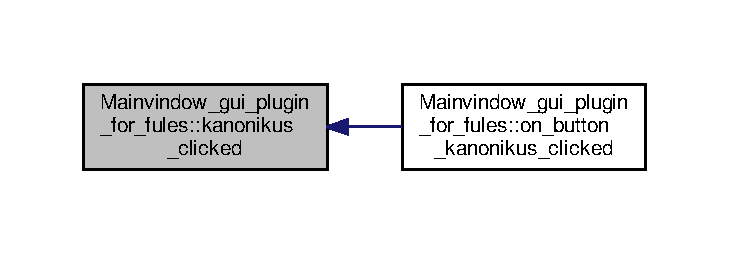
\includegraphics[width=350pt]{classMainvindow__gui__plugin__for__fules_a4ca08e417e9b4784db455ed9016870cc_icgraph}
\end{center}
\end{figure}
\mbox{\Hypertarget{classMainvindow__gui__plugin__for__fules_a69be0da66c49005cb7178c140b53dccb}\label{classMainvindow__gui__plugin__for__fules_a69be0da66c49005cb7178c140b53dccb}} 
\index{Mainvindow\+\_\+gui\+\_\+plugin\+\_\+for\+\_\+fules@{Mainvindow\+\_\+gui\+\_\+plugin\+\_\+for\+\_\+fules}!make\+\_\+indulo\+\_\+matrix@{make\+\_\+indulo\+\_\+matrix}}
\index{make\+\_\+indulo\+\_\+matrix@{make\+\_\+indulo\+\_\+matrix}!Mainvindow\+\_\+gui\+\_\+plugin\+\_\+for\+\_\+fules@{Mainvindow\+\_\+gui\+\_\+plugin\+\_\+for\+\_\+fules}}
\subsubsection{\texorpdfstring{make\+\_\+indulo\+\_\+matrix}{make\_indulo\_matrix}}
{\footnotesize\ttfamily void Mainvindow\+\_\+gui\+\_\+plugin\+\_\+for\+\_\+fules\+::make\+\_\+indulo\+\_\+matrix (\begin{DoxyParamCaption}{ }\end{DoxyParamCaption})\hspace{0.3cm}{\ttfamily [signal]}}

Here is the caller graph for this function\+:\nopagebreak
\begin{figure}[H]
\begin{center}
\leavevmode
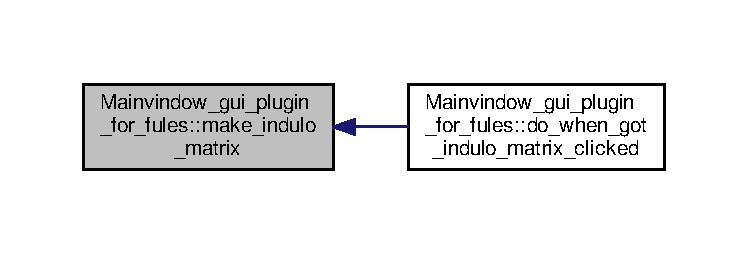
\includegraphics[width=350pt]{classMainvindow__gui__plugin__for__fules_a69be0da66c49005cb7178c140b53dccb_icgraph}
\end{center}
\end{figure}
\mbox{\Hypertarget{classMainvindow__gui__plugin__for__fules_ad57320bcd6e0f8353254601919b980b9}\label{classMainvindow__gui__plugin__for__fules_ad57320bcd6e0f8353254601919b980b9}} 
\index{Mainvindow\+\_\+gui\+\_\+plugin\+\_\+for\+\_\+fules@{Mainvindow\+\_\+gui\+\_\+plugin\+\_\+for\+\_\+fules}!make\+\_\+kanonikus@{make\+\_\+kanonikus}}
\index{make\+\_\+kanonikus@{make\+\_\+kanonikus}!Mainvindow\+\_\+gui\+\_\+plugin\+\_\+for\+\_\+fules@{Mainvindow\+\_\+gui\+\_\+plugin\+\_\+for\+\_\+fules}}
\subsubsection{\texorpdfstring{make\+\_\+kanonikus}{make\_kanonikus}}
{\footnotesize\ttfamily void Mainvindow\+\_\+gui\+\_\+plugin\+\_\+for\+\_\+fules\+::make\+\_\+kanonikus (\begin{DoxyParamCaption}{ }\end{DoxyParamCaption})\hspace{0.3cm}{\ttfamily [signal]}}

Here is the caller graph for this function\+:\nopagebreak
\begin{figure}[H]
\begin{center}
\leavevmode
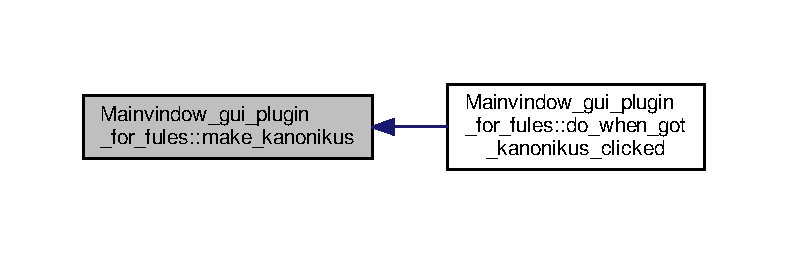
\includegraphics[width=350pt]{classMainvindow__gui__plugin__for__fules_ad57320bcd6e0f8353254601919b980b9_icgraph}
\end{center}
\end{figure}
\mbox{\Hypertarget{classMainvindow__gui__plugin__for__fules_abfd45e12e05f78b189c4ad00f7fb6930}\label{classMainvindow__gui__plugin__for__fules_abfd45e12e05f78b189c4ad00f7fb6930}} 
\index{Mainvindow\+\_\+gui\+\_\+plugin\+\_\+for\+\_\+fules@{Mainvindow\+\_\+gui\+\_\+plugin\+\_\+for\+\_\+fules}!Name@{Name}}
\index{Name@{Name}!Mainvindow\+\_\+gui\+\_\+plugin\+\_\+for\+\_\+fules@{Mainvindow\+\_\+gui\+\_\+plugin\+\_\+for\+\_\+fules}}
\subsubsection{\texorpdfstring{Name()}{Name()}}
{\footnotesize\ttfamily Q\+String Mainvindow\+\_\+gui\+\_\+plugin\+\_\+for\+\_\+fules\+::\+Name (\begin{DoxyParamCaption}{ }\end{DoxyParamCaption}) const\hspace{0.3cm}{\ttfamily [override]}, {\ttfamily [virtual]}}



Implements \hyperlink{classMainwindow__Gui__Plugin__Interface_a5cbc7bb0e3bb477472b91f65e916db8e}{Mainwindow\+\_\+\+Gui\+\_\+\+Plugin\+\_\+\+Interface}.



Definition at line 56 of file mainvindow\+\_\+gui\+\_\+plugin\+\_\+for\+\_\+fules.\+cpp.

\mbox{\Hypertarget{classMainvindow__gui__plugin__for__fules_aea9911335d30ac911adf04aa5ccfd8ee}\label{classMainvindow__gui__plugin__for__fules_aea9911335d30ac911adf04aa5ccfd8ee}} 
\index{Mainvindow\+\_\+gui\+\_\+plugin\+\_\+for\+\_\+fules@{Mainvindow\+\_\+gui\+\_\+plugin\+\_\+for\+\_\+fules}!on\+\_\+button\+\_\+indulo\+\_\+matrix\+\_\+clicked@{on\+\_\+button\+\_\+indulo\+\_\+matrix\+\_\+clicked}}
\index{on\+\_\+button\+\_\+indulo\+\_\+matrix\+\_\+clicked@{on\+\_\+button\+\_\+indulo\+\_\+matrix\+\_\+clicked}!Mainvindow\+\_\+gui\+\_\+plugin\+\_\+for\+\_\+fules@{Mainvindow\+\_\+gui\+\_\+plugin\+\_\+for\+\_\+fules}}
\subsubsection{\texorpdfstring{on\+\_\+button\+\_\+indulo\+\_\+matrix\+\_\+clicked}{on\_button\_indulo\_matrix\_clicked}}
{\footnotesize\ttfamily void Mainvindow\+\_\+gui\+\_\+plugin\+\_\+for\+\_\+fules\+::on\+\_\+button\+\_\+indulo\+\_\+matrix\+\_\+clicked (\begin{DoxyParamCaption}{ }\end{DoxyParamCaption})\hspace{0.3cm}{\ttfamily [private]}, {\ttfamily [slot]}}



Definition at line 71 of file mainvindow\+\_\+gui\+\_\+plugin\+\_\+for\+\_\+fules.\+cpp.

\mbox{\Hypertarget{classMainvindow__gui__plugin__for__fules_adc6ad081195bda78f2d2c93736aba030}\label{classMainvindow__gui__plugin__for__fules_adc6ad081195bda78f2d2c93736aba030}} 
\index{Mainvindow\+\_\+gui\+\_\+plugin\+\_\+for\+\_\+fules@{Mainvindow\+\_\+gui\+\_\+plugin\+\_\+for\+\_\+fules}!on\+\_\+button\+\_\+kanonikus\+\_\+clicked@{on\+\_\+button\+\_\+kanonikus\+\_\+clicked}}
\index{on\+\_\+button\+\_\+kanonikus\+\_\+clicked@{on\+\_\+button\+\_\+kanonikus\+\_\+clicked}!Mainvindow\+\_\+gui\+\_\+plugin\+\_\+for\+\_\+fules@{Mainvindow\+\_\+gui\+\_\+plugin\+\_\+for\+\_\+fules}}
\subsubsection{\texorpdfstring{on\+\_\+button\+\_\+kanonikus\+\_\+clicked}{on\_button\_kanonikus\_clicked}}
{\footnotesize\ttfamily void Mainvindow\+\_\+gui\+\_\+plugin\+\_\+for\+\_\+fules\+::on\+\_\+button\+\_\+kanonikus\+\_\+clicked (\begin{DoxyParamCaption}{ }\end{DoxyParamCaption})\hspace{0.3cm}{\ttfamily [private]}, {\ttfamily [slot]}}



Definition at line 110 of file mainvindow\+\_\+gui\+\_\+plugin\+\_\+for\+\_\+fules.\+cpp.

\mbox{\Hypertarget{classMainvindow__gui__plugin__for__fules_ae833c3ac5845928744df35c255c80a76}\label{classMainvindow__gui__plugin__for__fules_ae833c3ac5845928744df35c255c80a76}} 
\index{Mainvindow\+\_\+gui\+\_\+plugin\+\_\+for\+\_\+fules@{Mainvindow\+\_\+gui\+\_\+plugin\+\_\+for\+\_\+fules}!on\+\_\+button\+\_\+kezd\+\_\+clicked@{on\+\_\+button\+\_\+kezd\+\_\+clicked}}
\index{on\+\_\+button\+\_\+kezd\+\_\+clicked@{on\+\_\+button\+\_\+kezd\+\_\+clicked}!Mainvindow\+\_\+gui\+\_\+plugin\+\_\+for\+\_\+fules@{Mainvindow\+\_\+gui\+\_\+plugin\+\_\+for\+\_\+fules}}
\subsubsection{\texorpdfstring{on\+\_\+button\+\_\+kezd\+\_\+clicked}{on\_button\_kezd\_clicked}}
{\footnotesize\ttfamily void Mainvindow\+\_\+gui\+\_\+plugin\+\_\+for\+\_\+fules\+::on\+\_\+button\+\_\+kezd\+\_\+clicked (\begin{DoxyParamCaption}{ }\end{DoxyParamCaption})\hspace{0.3cm}{\ttfamily [private]}, {\ttfamily [slot]}}



Definition at line 84 of file mainvindow\+\_\+gui\+\_\+plugin\+\_\+for\+\_\+fules.\+cpp.

\mbox{\Hypertarget{classMainvindow__gui__plugin__for__fules_ae30db934e0e08f96cebd31c051fc43c5}\label{classMainvindow__gui__plugin__for__fules_ae30db934e0e08f96cebd31c051fc43c5}} 
\index{Mainvindow\+\_\+gui\+\_\+plugin\+\_\+for\+\_\+fules@{Mainvindow\+\_\+gui\+\_\+plugin\+\_\+for\+\_\+fules}!on\+\_\+button\+\_\+szamol\+\_\+clicked@{on\+\_\+button\+\_\+szamol\+\_\+clicked}}
\index{on\+\_\+button\+\_\+szamol\+\_\+clicked@{on\+\_\+button\+\_\+szamol\+\_\+clicked}!Mainvindow\+\_\+gui\+\_\+plugin\+\_\+for\+\_\+fules@{Mainvindow\+\_\+gui\+\_\+plugin\+\_\+for\+\_\+fules}}
\subsubsection{\texorpdfstring{on\+\_\+button\+\_\+szamol\+\_\+clicked}{on\_button\_szamol\_clicked}}
{\footnotesize\ttfamily void Mainvindow\+\_\+gui\+\_\+plugin\+\_\+for\+\_\+fules\+::on\+\_\+button\+\_\+szamol\+\_\+clicked (\begin{DoxyParamCaption}{ }\end{DoxyParamCaption})\hspace{0.3cm}{\ttfamily [private]}, {\ttfamily [slot]}}



Definition at line 63 of file mainvindow\+\_\+gui\+\_\+plugin\+\_\+for\+\_\+fules.\+cpp.

\mbox{\Hypertarget{classMainvindow__gui__plugin__for__fules_a40fb3f212d108731599d9a3e106ad65b}\label{classMainvindow__gui__plugin__for__fules_a40fb3f212d108731599d9a3e106ad65b}} 
\index{Mainvindow\+\_\+gui\+\_\+plugin\+\_\+for\+\_\+fules@{Mainvindow\+\_\+gui\+\_\+plugin\+\_\+for\+\_\+fules}!on\+\_\+radio\+Button\+\_\+2\+\_\+toggled@{on\+\_\+radio\+Button\+\_\+2\+\_\+toggled}}
\index{on\+\_\+radio\+Button\+\_\+2\+\_\+toggled@{on\+\_\+radio\+Button\+\_\+2\+\_\+toggled}!Mainvindow\+\_\+gui\+\_\+plugin\+\_\+for\+\_\+fules@{Mainvindow\+\_\+gui\+\_\+plugin\+\_\+for\+\_\+fules}}
\subsubsection{\texorpdfstring{on\+\_\+radio\+Button\+\_\+2\+\_\+toggled}{on\_radioButton\_2\_toggled}}
{\footnotesize\ttfamily void Mainvindow\+\_\+gui\+\_\+plugin\+\_\+for\+\_\+fules\+::on\+\_\+radio\+Button\+\_\+2\+\_\+toggled (\begin{DoxyParamCaption}\item[{bool}]{checked }\end{DoxyParamCaption})\hspace{0.3cm}{\ttfamily [private]}, {\ttfamily [slot]}}



Definition at line 137 of file mainvindow\+\_\+gui\+\_\+plugin\+\_\+for\+\_\+fules.\+cpp.

\mbox{\Hypertarget{classMainvindow__gui__plugin__for__fules_a8c33c824b142bea8995e3dd12f081f21}\label{classMainvindow__gui__plugin__for__fules_a8c33c824b142bea8995e3dd12f081f21}} 
\index{Mainvindow\+\_\+gui\+\_\+plugin\+\_\+for\+\_\+fules@{Mainvindow\+\_\+gui\+\_\+plugin\+\_\+for\+\_\+fules}!on\+\_\+radio\+Button\+\_\+toggled@{on\+\_\+radio\+Button\+\_\+toggled}}
\index{on\+\_\+radio\+Button\+\_\+toggled@{on\+\_\+radio\+Button\+\_\+toggled}!Mainvindow\+\_\+gui\+\_\+plugin\+\_\+for\+\_\+fules@{Mainvindow\+\_\+gui\+\_\+plugin\+\_\+for\+\_\+fules}}
\subsubsection{\texorpdfstring{on\+\_\+radio\+Button\+\_\+toggled}{on\_radioButton\_toggled}}
{\footnotesize\ttfamily void Mainvindow\+\_\+gui\+\_\+plugin\+\_\+for\+\_\+fules\+::on\+\_\+radio\+Button\+\_\+toggled (\begin{DoxyParamCaption}\item[{bool}]{checked }\end{DoxyParamCaption})\hspace{0.3cm}{\ttfamily [private]}, {\ttfamily [slot]}}



Definition at line 148 of file mainvindow\+\_\+gui\+\_\+plugin\+\_\+for\+\_\+fules.\+cpp.

\mbox{\Hypertarget{classMainvindow__gui__plugin__for__fules_a04e1668bac22f62c014954222d19f2ac}\label{classMainvindow__gui__plugin__for__fules_a04e1668bac22f62c014954222d19f2ac}} 
\index{Mainvindow\+\_\+gui\+\_\+plugin\+\_\+for\+\_\+fules@{Mainvindow\+\_\+gui\+\_\+plugin\+\_\+for\+\_\+fules}!sor\+\_\+oszlop\+\_\+db@{sor\+\_\+oszlop\+\_\+db}}
\index{sor\+\_\+oszlop\+\_\+db@{sor\+\_\+oszlop\+\_\+db}!Mainvindow\+\_\+gui\+\_\+plugin\+\_\+for\+\_\+fules@{Mainvindow\+\_\+gui\+\_\+plugin\+\_\+for\+\_\+fules}}
\subsubsection{\texorpdfstring{sor\+\_\+oszlop\+\_\+db}{sor\_oszlop\_db}}
{\footnotesize\ttfamily void Mainvindow\+\_\+gui\+\_\+plugin\+\_\+for\+\_\+fules\+::sor\+\_\+oszlop\+\_\+db (\begin{DoxyParamCaption}\item[{int}]{,  }\item[{int}]{ }\end{DoxyParamCaption})\hspace{0.3cm}{\ttfamily [signal]}}

Here is the caller graph for this function\+:\nopagebreak
\begin{figure}[H]
\begin{center}
\leavevmode
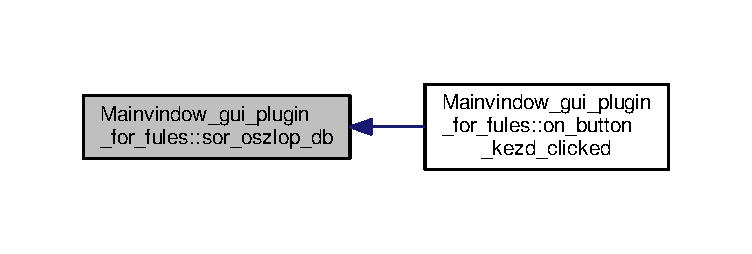
\includegraphics[width=350pt]{classMainvindow__gui__plugin__for__fules_a04e1668bac22f62c014954222d19f2ac_icgraph}
\end{center}
\end{figure}
\mbox{\Hypertarget{classMainvindow__gui__plugin__for__fules_ab44bcc45064b346477fef5df26a119cc}\label{classMainvindow__gui__plugin__for__fules_ab44bcc45064b346477fef5df26a119cc}} 
\index{Mainvindow\+\_\+gui\+\_\+plugin\+\_\+for\+\_\+fules@{Mainvindow\+\_\+gui\+\_\+plugin\+\_\+for\+\_\+fules}!szamol@{szamol}}
\index{szamol@{szamol}!Mainvindow\+\_\+gui\+\_\+plugin\+\_\+for\+\_\+fules@{Mainvindow\+\_\+gui\+\_\+plugin\+\_\+for\+\_\+fules}}
\subsubsection{\texorpdfstring{szamol}{szamol}}
{\footnotesize\ttfamily void Mainvindow\+\_\+gui\+\_\+plugin\+\_\+for\+\_\+fules\+::szamol (\begin{DoxyParamCaption}{ }\end{DoxyParamCaption})\hspace{0.3cm}{\ttfamily [signal]}}

Here is the caller graph for this function\+:\nopagebreak
\begin{figure}[H]
\begin{center}
\leavevmode
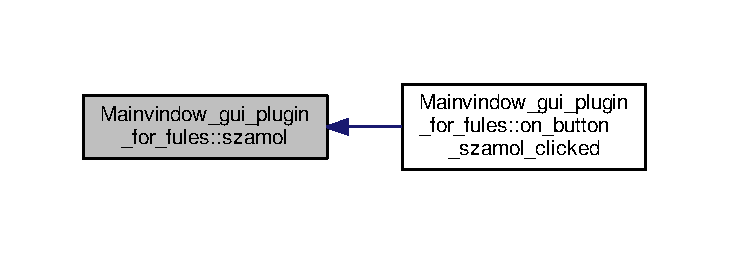
\includegraphics[width=350pt]{classMainvindow__gui__plugin__for__fules_ab44bcc45064b346477fef5df26a119cc_icgraph}
\end{center}
\end{figure}
\mbox{\Hypertarget{classMainvindow__gui__plugin__for__fules_a080c54bd4e8e65ffcaacad58e900248a}\label{classMainvindow__gui__plugin__for__fules_a080c54bd4e8e65ffcaacad58e900248a}} 
\index{Mainvindow\+\_\+gui\+\_\+plugin\+\_\+for\+\_\+fules@{Mainvindow\+\_\+gui\+\_\+plugin\+\_\+for\+\_\+fules}!vegigszamol@{vegigszamol}}
\index{vegigszamol@{vegigszamol}!Mainvindow\+\_\+gui\+\_\+plugin\+\_\+for\+\_\+fules@{Mainvindow\+\_\+gui\+\_\+plugin\+\_\+for\+\_\+fules}}
\subsubsection{\texorpdfstring{vegigszamol}{vegigszamol}}
{\footnotesize\ttfamily void Mainvindow\+\_\+gui\+\_\+plugin\+\_\+for\+\_\+fules\+::vegigszamol (\begin{DoxyParamCaption}\item[{bool}]{vegigszamolando }\end{DoxyParamCaption})\hspace{0.3cm}{\ttfamily [signal]}}

Here is the caller graph for this function\+:\nopagebreak
\begin{figure}[H]
\begin{center}
\leavevmode
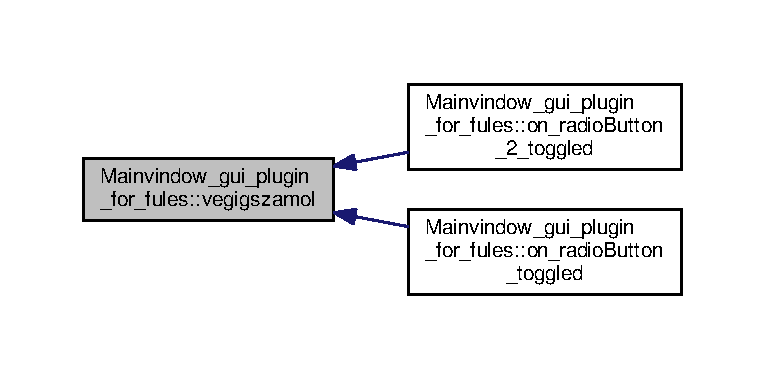
\includegraphics[width=350pt]{classMainvindow__gui__plugin__for__fules_a080c54bd4e8e65ffcaacad58e900248a_icgraph}
\end{center}
\end{figure}


\subsection{Member Data Documentation}
\mbox{\Hypertarget{classMainvindow__gui__plugin__for__fules_aea0a3b7f00e651f970723dab3338240d}\label{classMainvindow__gui__plugin__for__fules_aea0a3b7f00e651f970723dab3338240d}} 
\index{Mainvindow\+\_\+gui\+\_\+plugin\+\_\+for\+\_\+fules@{Mainvindow\+\_\+gui\+\_\+plugin\+\_\+for\+\_\+fules}!non\+\_\+numeric\+\_\+delegate@{non\+\_\+numeric\+\_\+delegate}}
\index{non\+\_\+numeric\+\_\+delegate@{non\+\_\+numeric\+\_\+delegate}!Mainvindow\+\_\+gui\+\_\+plugin\+\_\+for\+\_\+fules@{Mainvindow\+\_\+gui\+\_\+plugin\+\_\+for\+\_\+fules}}
\subsubsection{\texorpdfstring{non\+\_\+numeric\+\_\+delegate}{non\_numeric\_delegate}}
{\footnotesize\ttfamily \hyperlink{classNon__numeric__Delegate__in__fules}{Non\+\_\+numeric\+\_\+\+Delegate\+\_\+in\+\_\+fules}$\ast$ Mainvindow\+\_\+gui\+\_\+plugin\+\_\+for\+\_\+fules\+::non\+\_\+numeric\+\_\+delegate\hspace{0.3cm}{\ttfamily [private]}}



Definition at line 66 of file mainvindow\+\_\+gui\+\_\+plugin\+\_\+for\+\_\+fules.\+h.

\mbox{\Hypertarget{classMainvindow__gui__plugin__for__fules_a6b1f4a0fae34535113840411223ccfa6}\label{classMainvindow__gui__plugin__for__fules_a6b1f4a0fae34535113840411223ccfa6}} 
\index{Mainvindow\+\_\+gui\+\_\+plugin\+\_\+for\+\_\+fules@{Mainvindow\+\_\+gui\+\_\+plugin\+\_\+for\+\_\+fules}!number\+\_\+delegator@{number\+\_\+delegator}}
\index{number\+\_\+delegator@{number\+\_\+delegator}!Mainvindow\+\_\+gui\+\_\+plugin\+\_\+for\+\_\+fules@{Mainvindow\+\_\+gui\+\_\+plugin\+\_\+for\+\_\+fules}}
\subsubsection{\texorpdfstring{number\+\_\+delegator}{number\_delegator}}
{\footnotesize\ttfamily \hyperlink{classDelegate__for__numbers__in__fules}{Delegate\+\_\+for\+\_\+numbers\+\_\+in\+\_\+fules}$\ast$ Mainvindow\+\_\+gui\+\_\+plugin\+\_\+for\+\_\+fules\+::number\+\_\+delegator\hspace{0.3cm}{\ttfamily [private]}}



Definition at line 65 of file mainvindow\+\_\+gui\+\_\+plugin\+\_\+for\+\_\+fules.\+h.

\mbox{\Hypertarget{classMainvindow__gui__plugin__for__fules_acdd8ed5ce96f1565bc722f1965faca67}\label{classMainvindow__gui__plugin__for__fules_acdd8ed5ce96f1565bc722f1965faca67}} 
\index{Mainvindow\+\_\+gui\+\_\+plugin\+\_\+for\+\_\+fules@{Mainvindow\+\_\+gui\+\_\+plugin\+\_\+for\+\_\+fules}!ui@{ui}}
\index{ui@{ui}!Mainvindow\+\_\+gui\+\_\+plugin\+\_\+for\+\_\+fules@{Mainvindow\+\_\+gui\+\_\+plugin\+\_\+for\+\_\+fules}}
\subsubsection{\texorpdfstring{ui}{ui}}
{\footnotesize\ttfamily Ui\+::\+Mainvindow\+\_\+gui\+\_\+plugin\+\_\+for\+\_\+fules$\ast$ Mainvindow\+\_\+gui\+\_\+plugin\+\_\+for\+\_\+fules\+::ui\hspace{0.3cm}{\ttfamily [private]}}



Definition at line 64 of file mainvindow\+\_\+gui\+\_\+plugin\+\_\+for\+\_\+fules.\+h.



The documentation for this class was generated from the following files\+:\begin{DoxyCompactItemize}
\item 
fules/\hyperlink{mainvindow__gui__plugin__for__fules_8h}{mainvindow\+\_\+gui\+\_\+plugin\+\_\+for\+\_\+fules.\+h}\item 
fules/\hyperlink{mainvindow__gui__plugin__for__fules_8cpp}{mainvindow\+\_\+gui\+\_\+plugin\+\_\+for\+\_\+fules.\+cpp}\end{DoxyCompactItemize}

\hypertarget{classMainWindow}{}\section{Main\+Window Class Reference}
\label{classMainWindow}\index{Main\+Window@{Main\+Window}}


{\ttfamily \#include $<$mainwindow.\+h$>$}



Inherits Q\+Main\+Window.

\subsection*{Public Member Functions}
\begin{DoxyCompactItemize}
\item 
\hyperlink{classMainWindow_a996c5a2b6f77944776856f08ec30858d}{Main\+Window} (Q\+Widget $\ast$parent=nullptr)
\item 
\hyperlink{classMainWindow_ae98d00a93bc118200eeef9f9bba1dba7}{$\sim$\+Main\+Window} ()
\end{DoxyCompactItemize}
\subsection*{Private Member Functions}
\begin{DoxyCompactItemize}
\item 
void \hyperlink{classMainWindow_a465314c6317877838dfe332838be19b2}{add\+\_\+menus} (Q\+Widget $\ast$parent\+\_\+)
\end{DoxyCompactItemize}
\subsection*{Private Attributes}
\begin{DoxyCompactItemize}
\item 
Q\+Menu $\ast$ \hyperlink{classMainWindow_a4844d3dbe9895a5e2e9dd86e44ebc68c}{gui\+\_\+plugin\+\_\+menu}
\item 
Q\+Menu $\ast$ \hyperlink{classMainWindow_a919b4e91bffc528a3a179066e764b585}{pivot\+\_\+plugin\+\_\+menu}
\item 
Q\+Menu $\ast$ \hyperlink{classMainWindow_a7e9ebcb30a5c1b52b333667d1846c39b}{result\+\_\+reporter\+\_\+plugin\+\_\+menu}
\item 
Q\+Menu $\ast$ \hyperlink{classMainWindow_a0124119ae5ce14b59e7ab9a93aae5c36}{db\+\_\+plugin\+\_\+menu}
\item 
Q\+Menu $\ast$ \hyperlink{classMainWindow_a27f95fb7021c28fafdef73ed5bddb225}{elmelet\+\_\+plugin\+\_\+menu}
\item 
Q\+Menu $\ast$ \hyperlink{classMainWindow_af9d894ce80a9a3beb435198d7c7bcb8d}{Settings\+\_\+menu}
\item 
Q\+Menu $\ast$ \hyperlink{classMainWindow_a2068ab7a73c3d08e80b4a2b2c7382388}{Help\+\_\+menu}
\item 
Q\+Stacked\+Widget $\ast$ \hyperlink{classMainWindow_a257f380476b4629d8a0b85fc3bca970e}{central\+\_\+widget}
\item 
Ui\+::\+Main\+Window $\ast$ \hyperlink{classMainWindow_a35466a70ed47252a0191168126a352a5}{ui}
\end{DoxyCompactItemize}
\subsection*{Friends}
\begin{DoxyCompactItemize}
\item 
class \hyperlink{classMainWindow_a9762517abc1c30aa1289cf8dc2560b3d}{gui\+\_\+plugin\+\_\+loader}
\item 
class \hyperlink{classMainWindow_a6ea4c13e2ee3a46ce7f59f0baaf4feca}{Pivot\+\_\+\+Selector\+\_\+\+Plugin\+\_\+\+Loader}
\item 
class \hyperlink{classMainWindow_a2ae02a3574508e653447a544639a0fe0}{exercise\+\_\+load\+\_\+plugin\+\_\+loader}
\item 
class \hyperlink{classMainWindow_acf22a6b2f20681439abffae3722aca85}{picture\+\_\+load\+\_\+plugin\+\_\+loader}
\item 
class \hyperlink{classMainWindow_a238e01801020c0ea22d30739cbfc35f1}{Result\+\_\+\+Report\+\_\+plugin\+\_\+\+Loader}
\item 
class \hyperlink{classMainWindow_aa57bcac61e09f9c999a2f048dc923409}{Simplex\+\_\+method\+\_\+calculator}
\end{DoxyCompactItemize}


\subsection{Detailed Description}


Definition at line 11 of file mainwindow.\+h.



\subsection{Constructor \& Destructor Documentation}
\mbox{\Hypertarget{classMainWindow_a996c5a2b6f77944776856f08ec30858d}\label{classMainWindow_a996c5a2b6f77944776856f08ec30858d}} 
\index{Main\+Window@{Main\+Window}!Main\+Window@{Main\+Window}}
\index{Main\+Window@{Main\+Window}!Main\+Window@{Main\+Window}}
\subsubsection{\texorpdfstring{Main\+Window()}{MainWindow()}}
{\footnotesize\ttfamily Main\+Window\+::\+Main\+Window (\begin{DoxyParamCaption}\item[{Q\+Widget $\ast$}]{parent = {\ttfamily nullptr} }\end{DoxyParamCaption})\hspace{0.3cm}{\ttfamily [explicit]}}



Definition at line 6 of file mainwindow.\+cpp.

\mbox{\Hypertarget{classMainWindow_ae98d00a93bc118200eeef9f9bba1dba7}\label{classMainWindow_ae98d00a93bc118200eeef9f9bba1dba7}} 
\index{Main\+Window@{Main\+Window}!````~Main\+Window@{$\sim$\+Main\+Window}}
\index{````~Main\+Window@{$\sim$\+Main\+Window}!Main\+Window@{Main\+Window}}
\subsubsection{\texorpdfstring{$\sim$\+Main\+Window()}{~MainWindow()}}
{\footnotesize\ttfamily Main\+Window\+::$\sim$\+Main\+Window (\begin{DoxyParamCaption}{ }\end{DoxyParamCaption})}



Definition at line 21 of file mainwindow.\+cpp.



\subsection{Member Function Documentation}
\mbox{\Hypertarget{classMainWindow_a465314c6317877838dfe332838be19b2}\label{classMainWindow_a465314c6317877838dfe332838be19b2}} 
\index{Main\+Window@{Main\+Window}!add\+\_\+menus@{add\+\_\+menus}}
\index{add\+\_\+menus@{add\+\_\+menus}!Main\+Window@{Main\+Window}}
\subsubsection{\texorpdfstring{add\+\_\+menus()}{add\_menus()}}
{\footnotesize\ttfamily void Main\+Window\+::add\+\_\+menus (\begin{DoxyParamCaption}\item[{Q\+Widget $\ast$}]{parent\+\_\+ }\end{DoxyParamCaption})\hspace{0.3cm}{\ttfamily [private]}}



Definition at line 28 of file mainwindow.\+cpp.

Here is the call graph for this function\+:\nopagebreak
\begin{figure}[H]
\begin{center}
\leavevmode
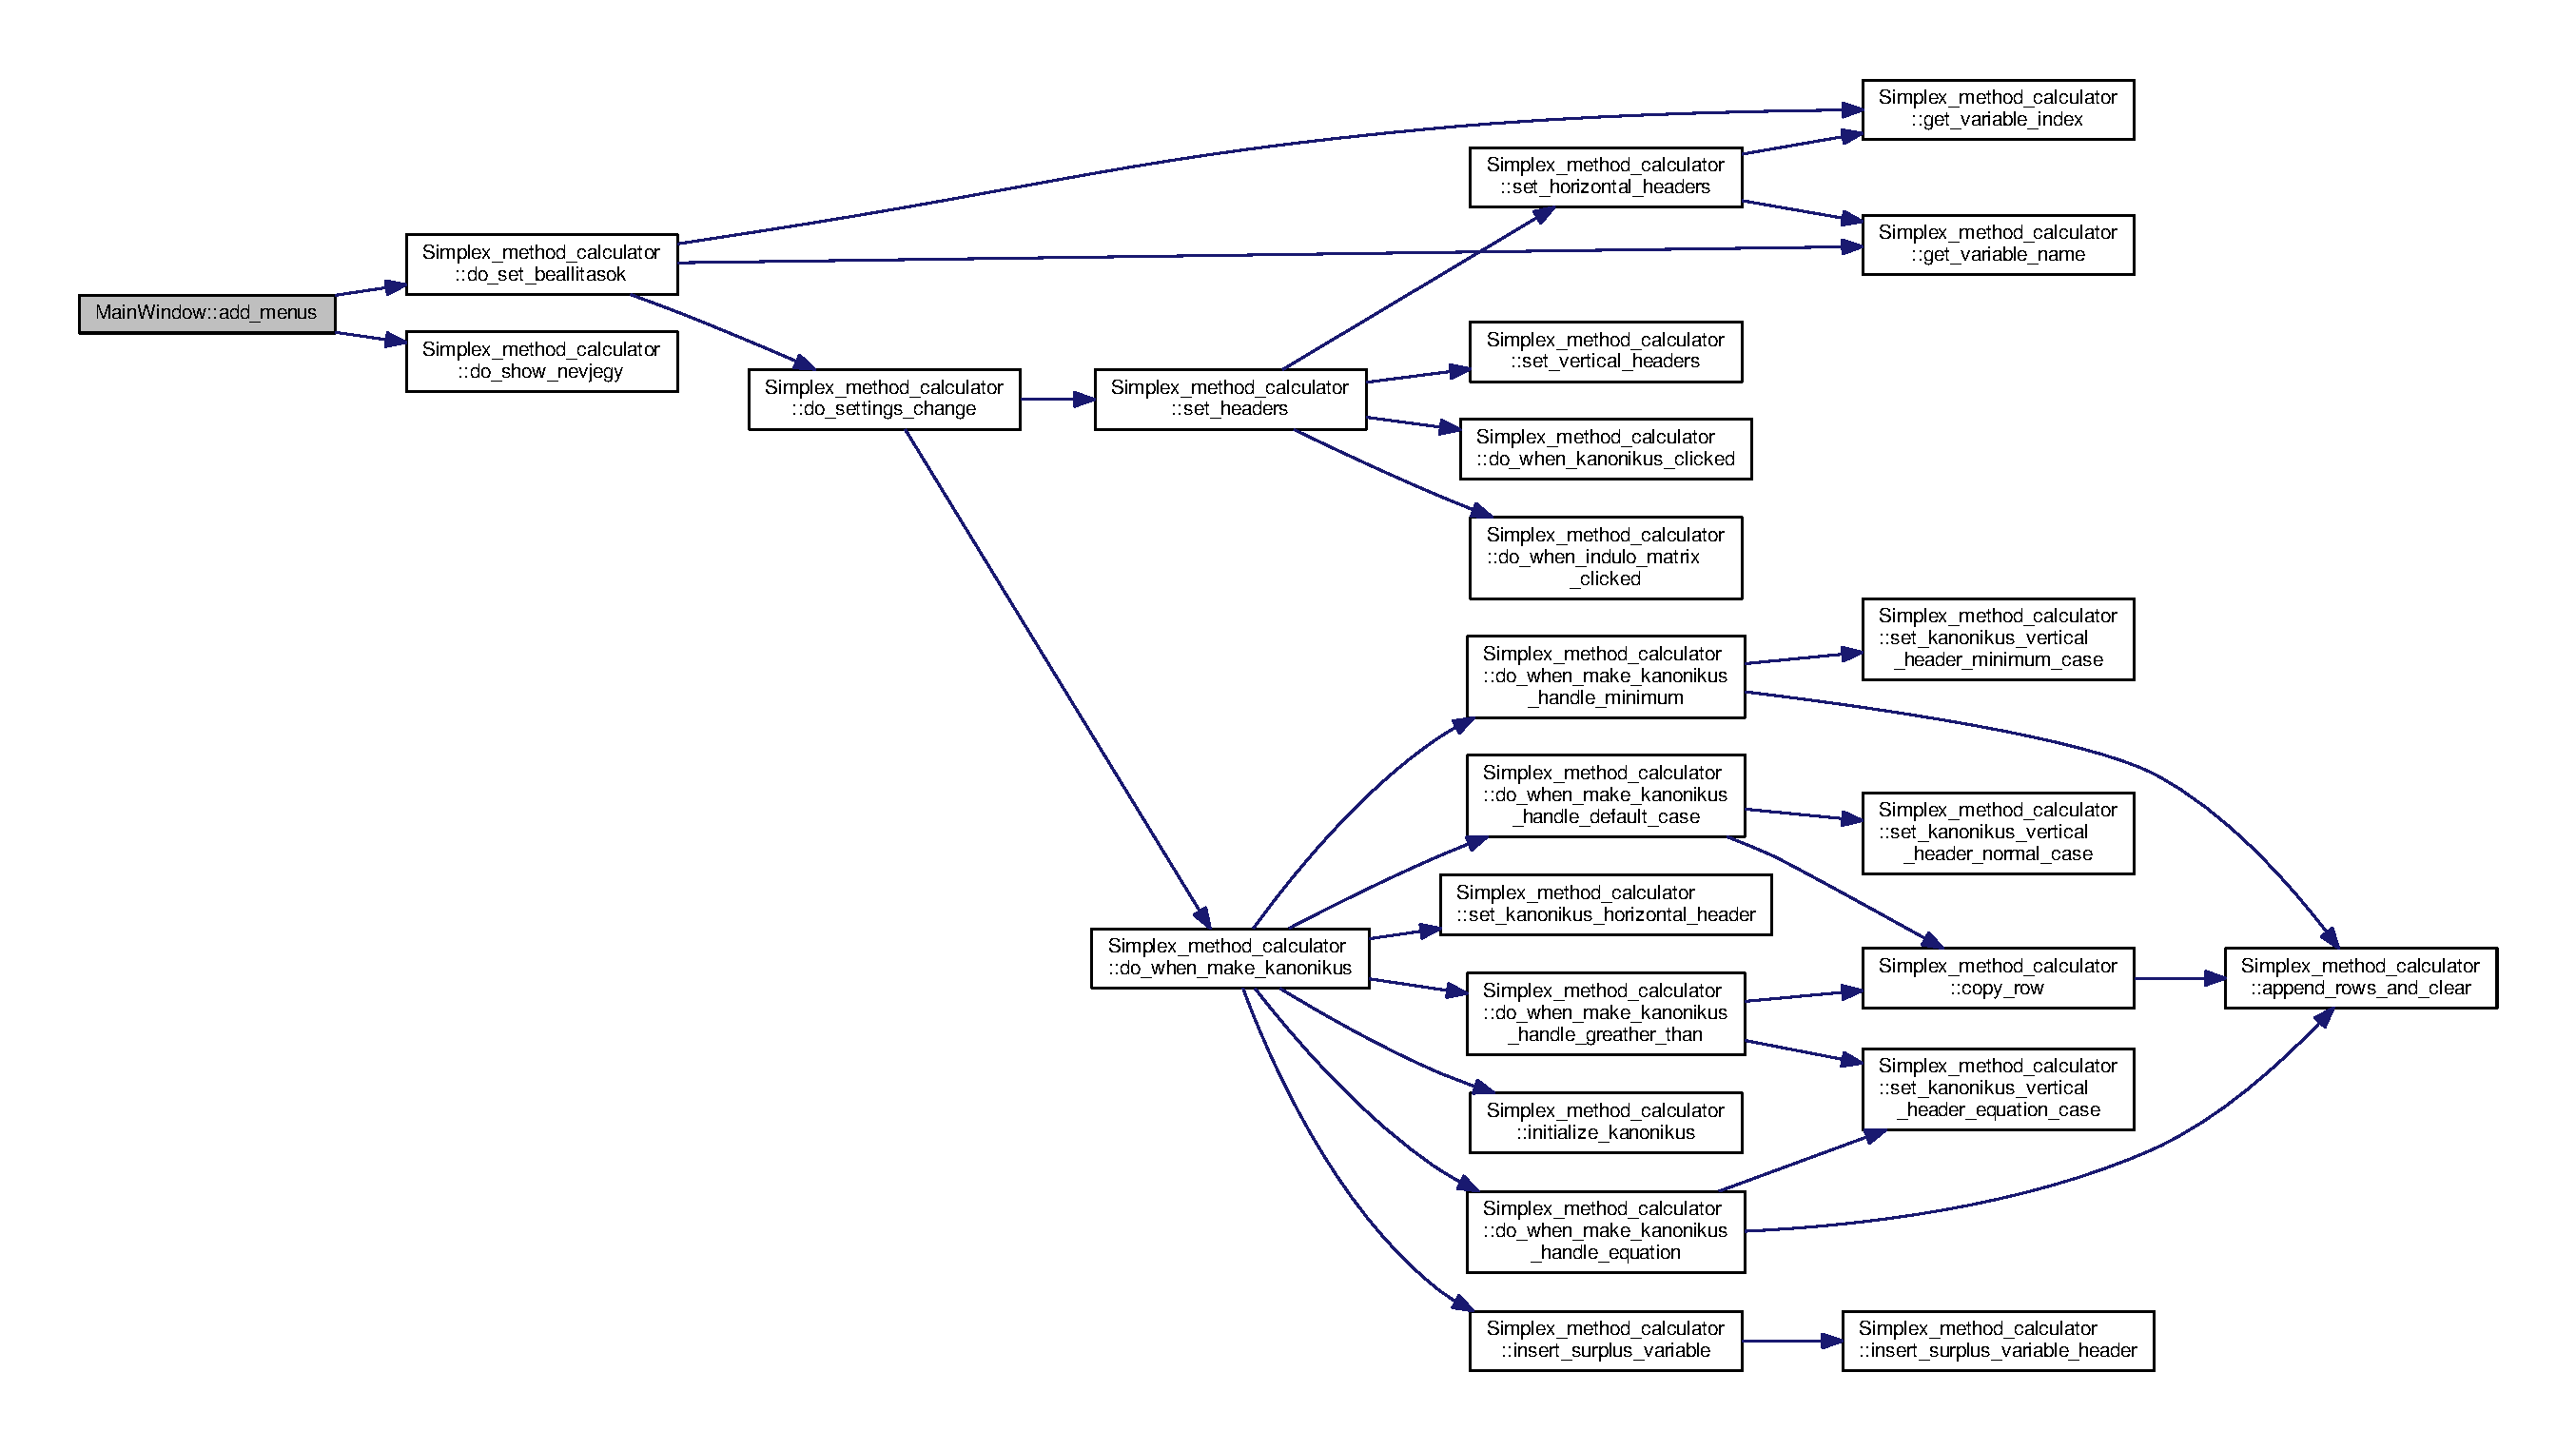
\includegraphics[width=350pt]{classMainWindow_a465314c6317877838dfe332838be19b2_cgraph}
\end{center}
\end{figure}
Here is the caller graph for this function\+:\nopagebreak
\begin{figure}[H]
\begin{center}
\leavevmode
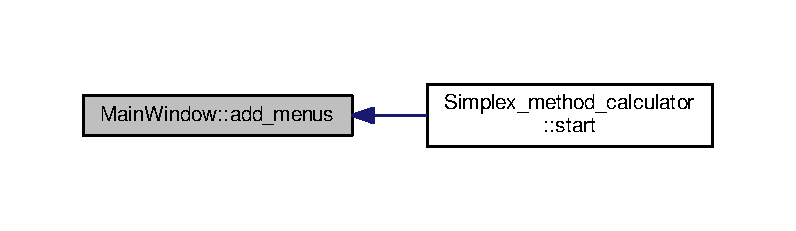
\includegraphics[width=350pt]{classMainWindow_a465314c6317877838dfe332838be19b2_icgraph}
\end{center}
\end{figure}


\subsection{Friends And Related Function Documentation}
\mbox{\Hypertarget{classMainWindow_a2ae02a3574508e653447a544639a0fe0}\label{classMainWindow_a2ae02a3574508e653447a544639a0fe0}} 
\index{Main\+Window@{Main\+Window}!exercise\+\_\+load\+\_\+plugin\+\_\+loader@{exercise\+\_\+load\+\_\+plugin\+\_\+loader}}
\index{exercise\+\_\+load\+\_\+plugin\+\_\+loader@{exercise\+\_\+load\+\_\+plugin\+\_\+loader}!Main\+Window@{Main\+Window}}
\subsubsection{\texorpdfstring{exercise\+\_\+load\+\_\+plugin\+\_\+loader}{exercise\_load\_plugin\_loader}}
{\footnotesize\ttfamily friend class \hyperlink{classexercise__load__plugin__loader}{exercise\+\_\+load\+\_\+plugin\+\_\+loader}\hspace{0.3cm}{\ttfamily [friend]}}



Definition at line 16 of file mainwindow.\+h.

\mbox{\Hypertarget{classMainWindow_a9762517abc1c30aa1289cf8dc2560b3d}\label{classMainWindow_a9762517abc1c30aa1289cf8dc2560b3d}} 
\index{Main\+Window@{Main\+Window}!gui\+\_\+plugin\+\_\+loader@{gui\+\_\+plugin\+\_\+loader}}
\index{gui\+\_\+plugin\+\_\+loader@{gui\+\_\+plugin\+\_\+loader}!Main\+Window@{Main\+Window}}
\subsubsection{\texorpdfstring{gui\+\_\+plugin\+\_\+loader}{gui\_plugin\_loader}}
{\footnotesize\ttfamily friend class \hyperlink{classgui__plugin__loader}{gui\+\_\+plugin\+\_\+loader}\hspace{0.3cm}{\ttfamily [friend]}}



Definition at line 14 of file mainwindow.\+h.

\mbox{\Hypertarget{classMainWindow_acf22a6b2f20681439abffae3722aca85}\label{classMainWindow_acf22a6b2f20681439abffae3722aca85}} 
\index{Main\+Window@{Main\+Window}!picture\+\_\+load\+\_\+plugin\+\_\+loader@{picture\+\_\+load\+\_\+plugin\+\_\+loader}}
\index{picture\+\_\+load\+\_\+plugin\+\_\+loader@{picture\+\_\+load\+\_\+plugin\+\_\+loader}!Main\+Window@{Main\+Window}}
\subsubsection{\texorpdfstring{picture\+\_\+load\+\_\+plugin\+\_\+loader}{picture\_load\_plugin\_loader}}
{\footnotesize\ttfamily friend class \hyperlink{classpicture__load__plugin__loader}{picture\+\_\+load\+\_\+plugin\+\_\+loader}\hspace{0.3cm}{\ttfamily [friend]}}



Definition at line 17 of file mainwindow.\+h.

\mbox{\Hypertarget{classMainWindow_a6ea4c13e2ee3a46ce7f59f0baaf4feca}\label{classMainWindow_a6ea4c13e2ee3a46ce7f59f0baaf4feca}} 
\index{Main\+Window@{Main\+Window}!Pivot\+\_\+\+Selector\+\_\+\+Plugin\+\_\+\+Loader@{Pivot\+\_\+\+Selector\+\_\+\+Plugin\+\_\+\+Loader}}
\index{Pivot\+\_\+\+Selector\+\_\+\+Plugin\+\_\+\+Loader@{Pivot\+\_\+\+Selector\+\_\+\+Plugin\+\_\+\+Loader}!Main\+Window@{Main\+Window}}
\subsubsection{\texorpdfstring{Pivot\+\_\+\+Selector\+\_\+\+Plugin\+\_\+\+Loader}{Pivot\_Selector\_Plugin\_Loader}}
{\footnotesize\ttfamily friend class \hyperlink{classPivot__Selector__Plugin__Loader}{Pivot\+\_\+\+Selector\+\_\+\+Plugin\+\_\+\+Loader}\hspace{0.3cm}{\ttfamily [friend]}}



Definition at line 15 of file mainwindow.\+h.

\mbox{\Hypertarget{classMainWindow_a238e01801020c0ea22d30739cbfc35f1}\label{classMainWindow_a238e01801020c0ea22d30739cbfc35f1}} 
\index{Main\+Window@{Main\+Window}!Result\+\_\+\+Report\+\_\+plugin\+\_\+\+Loader@{Result\+\_\+\+Report\+\_\+plugin\+\_\+\+Loader}}
\index{Result\+\_\+\+Report\+\_\+plugin\+\_\+\+Loader@{Result\+\_\+\+Report\+\_\+plugin\+\_\+\+Loader}!Main\+Window@{Main\+Window}}
\subsubsection{\texorpdfstring{Result\+\_\+\+Report\+\_\+plugin\+\_\+\+Loader}{Result\_Report\_plugin\_Loader}}
{\footnotesize\ttfamily friend class \hyperlink{classResult__Report__plugin__Loader}{Result\+\_\+\+Report\+\_\+plugin\+\_\+\+Loader}\hspace{0.3cm}{\ttfamily [friend]}}



Definition at line 18 of file mainwindow.\+h.

\mbox{\Hypertarget{classMainWindow_aa57bcac61e09f9c999a2f048dc923409}\label{classMainWindow_aa57bcac61e09f9c999a2f048dc923409}} 
\index{Main\+Window@{Main\+Window}!Simplex\+\_\+method\+\_\+calculator@{Simplex\+\_\+method\+\_\+calculator}}
\index{Simplex\+\_\+method\+\_\+calculator@{Simplex\+\_\+method\+\_\+calculator}!Main\+Window@{Main\+Window}}
\subsubsection{\texorpdfstring{Simplex\+\_\+method\+\_\+calculator}{Simplex\_method\_calculator}}
{\footnotesize\ttfamily friend class \hyperlink{classSimplex__method__calculator}{Simplex\+\_\+method\+\_\+calculator}\hspace{0.3cm}{\ttfamily [friend]}}



Definition at line 19 of file mainwindow.\+h.



\subsection{Member Data Documentation}
\mbox{\Hypertarget{classMainWindow_a257f380476b4629d8a0b85fc3bca970e}\label{classMainWindow_a257f380476b4629d8a0b85fc3bca970e}} 
\index{Main\+Window@{Main\+Window}!central\+\_\+widget@{central\+\_\+widget}}
\index{central\+\_\+widget@{central\+\_\+widget}!Main\+Window@{Main\+Window}}
\subsubsection{\texorpdfstring{central\+\_\+widget}{central\_widget}}
{\footnotesize\ttfamily Q\+Stacked\+Widget$\ast$ Main\+Window\+::central\+\_\+widget\hspace{0.3cm}{\ttfamily [private]}}



Definition at line 35 of file mainwindow.\+h.

\mbox{\Hypertarget{classMainWindow_a0124119ae5ce14b59e7ab9a93aae5c36}\label{classMainWindow_a0124119ae5ce14b59e7ab9a93aae5c36}} 
\index{Main\+Window@{Main\+Window}!db\+\_\+plugin\+\_\+menu@{db\+\_\+plugin\+\_\+menu}}
\index{db\+\_\+plugin\+\_\+menu@{db\+\_\+plugin\+\_\+menu}!Main\+Window@{Main\+Window}}
\subsubsection{\texorpdfstring{db\+\_\+plugin\+\_\+menu}{db\_plugin\_menu}}
{\footnotesize\ttfamily Q\+Menu$\ast$ Main\+Window\+::db\+\_\+plugin\+\_\+menu\hspace{0.3cm}{\ttfamily [private]}}



Definition at line 31 of file mainwindow.\+h.

\mbox{\Hypertarget{classMainWindow_a27f95fb7021c28fafdef73ed5bddb225}\label{classMainWindow_a27f95fb7021c28fafdef73ed5bddb225}} 
\index{Main\+Window@{Main\+Window}!elmelet\+\_\+plugin\+\_\+menu@{elmelet\+\_\+plugin\+\_\+menu}}
\index{elmelet\+\_\+plugin\+\_\+menu@{elmelet\+\_\+plugin\+\_\+menu}!Main\+Window@{Main\+Window}}
\subsubsection{\texorpdfstring{elmelet\+\_\+plugin\+\_\+menu}{elmelet\_plugin\_menu}}
{\footnotesize\ttfamily Q\+Menu$\ast$ Main\+Window\+::elmelet\+\_\+plugin\+\_\+menu\hspace{0.3cm}{\ttfamily [private]}}



Definition at line 32 of file mainwindow.\+h.

\mbox{\Hypertarget{classMainWindow_a4844d3dbe9895a5e2e9dd86e44ebc68c}\label{classMainWindow_a4844d3dbe9895a5e2e9dd86e44ebc68c}} 
\index{Main\+Window@{Main\+Window}!gui\+\_\+plugin\+\_\+menu@{gui\+\_\+plugin\+\_\+menu}}
\index{gui\+\_\+plugin\+\_\+menu@{gui\+\_\+plugin\+\_\+menu}!Main\+Window@{Main\+Window}}
\subsubsection{\texorpdfstring{gui\+\_\+plugin\+\_\+menu}{gui\_plugin\_menu}}
{\footnotesize\ttfamily Q\+Menu$\ast$ Main\+Window\+::gui\+\_\+plugin\+\_\+menu\hspace{0.3cm}{\ttfamily [private]}}



Definition at line 28 of file mainwindow.\+h.

\mbox{\Hypertarget{classMainWindow_a2068ab7a73c3d08e80b4a2b2c7382388}\label{classMainWindow_a2068ab7a73c3d08e80b4a2b2c7382388}} 
\index{Main\+Window@{Main\+Window}!Help\+\_\+menu@{Help\+\_\+menu}}
\index{Help\+\_\+menu@{Help\+\_\+menu}!Main\+Window@{Main\+Window}}
\subsubsection{\texorpdfstring{Help\+\_\+menu}{Help\_menu}}
{\footnotesize\ttfamily Q\+Menu$\ast$ Main\+Window\+::\+Help\+\_\+menu\hspace{0.3cm}{\ttfamily [private]}}



Definition at line 34 of file mainwindow.\+h.

\mbox{\Hypertarget{classMainWindow_a919b4e91bffc528a3a179066e764b585}\label{classMainWindow_a919b4e91bffc528a3a179066e764b585}} 
\index{Main\+Window@{Main\+Window}!pivot\+\_\+plugin\+\_\+menu@{pivot\+\_\+plugin\+\_\+menu}}
\index{pivot\+\_\+plugin\+\_\+menu@{pivot\+\_\+plugin\+\_\+menu}!Main\+Window@{Main\+Window}}
\subsubsection{\texorpdfstring{pivot\+\_\+plugin\+\_\+menu}{pivot\_plugin\_menu}}
{\footnotesize\ttfamily Q\+Menu$\ast$ Main\+Window\+::pivot\+\_\+plugin\+\_\+menu\hspace{0.3cm}{\ttfamily [private]}}



Definition at line 29 of file mainwindow.\+h.

\mbox{\Hypertarget{classMainWindow_a7e9ebcb30a5c1b52b333667d1846c39b}\label{classMainWindow_a7e9ebcb30a5c1b52b333667d1846c39b}} 
\index{Main\+Window@{Main\+Window}!result\+\_\+reporter\+\_\+plugin\+\_\+menu@{result\+\_\+reporter\+\_\+plugin\+\_\+menu}}
\index{result\+\_\+reporter\+\_\+plugin\+\_\+menu@{result\+\_\+reporter\+\_\+plugin\+\_\+menu}!Main\+Window@{Main\+Window}}
\subsubsection{\texorpdfstring{result\+\_\+reporter\+\_\+plugin\+\_\+menu}{result\_reporter\_plugin\_menu}}
{\footnotesize\ttfamily Q\+Menu$\ast$ Main\+Window\+::result\+\_\+reporter\+\_\+plugin\+\_\+menu\hspace{0.3cm}{\ttfamily [private]}}



Definition at line 30 of file mainwindow.\+h.

\mbox{\Hypertarget{classMainWindow_af9d894ce80a9a3beb435198d7c7bcb8d}\label{classMainWindow_af9d894ce80a9a3beb435198d7c7bcb8d}} 
\index{Main\+Window@{Main\+Window}!Settings\+\_\+menu@{Settings\+\_\+menu}}
\index{Settings\+\_\+menu@{Settings\+\_\+menu}!Main\+Window@{Main\+Window}}
\subsubsection{\texorpdfstring{Settings\+\_\+menu}{Settings\_menu}}
{\footnotesize\ttfamily Q\+Menu$\ast$ Main\+Window\+::\+Settings\+\_\+menu\hspace{0.3cm}{\ttfamily [private]}}



Definition at line 33 of file mainwindow.\+h.

\mbox{\Hypertarget{classMainWindow_a35466a70ed47252a0191168126a352a5}\label{classMainWindow_a35466a70ed47252a0191168126a352a5}} 
\index{Main\+Window@{Main\+Window}!ui@{ui}}
\index{ui@{ui}!Main\+Window@{Main\+Window}}
\subsubsection{\texorpdfstring{ui}{ui}}
{\footnotesize\ttfamily Ui\+::\+Main\+Window$\ast$ Main\+Window\+::ui\hspace{0.3cm}{\ttfamily [private]}}



Definition at line 43 of file mainwindow.\+h.



The documentation for this class was generated from the following files\+:\begin{DoxyCompactItemize}
\item 
simplex\+\_\+app/\hyperlink{mainwindow_8h}{mainwindow.\+h}\item 
simplex\+\_\+app/\hyperlink{mainwindow_8cpp}{mainwindow.\+cpp}\end{DoxyCompactItemize}

\hypertarget{classMainwindow__Gui__Plugin__Interface}{}\section{Mainwindow\+\_\+\+Gui\+\_\+\+Plugin\+\_\+\+Interface Class Reference}
\label{classMainwindow__Gui__Plugin__Interface}\index{Mainwindow\+\_\+\+Gui\+\_\+\+Plugin\+\_\+\+Interface@{Mainwindow\+\_\+\+Gui\+\_\+\+Plugin\+\_\+\+Interface}}


{\ttfamily \#include $<$mainwindow\+\_\+gui\+\_\+plugin\+\_\+interface.\+h$>$}



Inheritance diagram for Mainwindow\+\_\+\+Gui\+\_\+\+Plugin\+\_\+\+Interface\+:\nopagebreak
\begin{figure}[H]
\begin{center}
\leavevmode
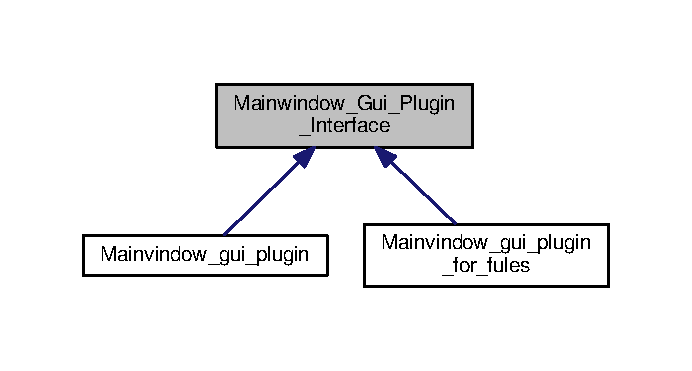
\includegraphics[width=332pt]{classMainwindow__Gui__Plugin__Interface__inherit__graph}
\end{center}
\end{figure}
\subsection*{Public Slots}
\begin{DoxyCompactItemize}
\item 
virtual void \hyperlink{classMainwindow__Gui__Plugin__Interface_a35df40a34eaf1d707d41db3f13862469}{do\+\_\+set\+\_\+indulo\+\_\+model\+\_\+view} (Q\+Standard\+Item\+Model $\ast$)=0
\item 
virtual void \hyperlink{classMainwindow__Gui__Plugin__Interface_a88a3437df47fa2957d31f487c22c5fad}{do\+\_\+set\+\_\+kanonikus\+\_\+alak\+\_\+model\+\_\+view} (Q\+Standard\+Item\+Model $\ast$)=0
\item 
virtual void \hyperlink{classMainwindow__Gui__Plugin__Interface_aeec7915d58c85d9d837c5faa50c9e567}{do\+\_\+set\+\_\+indulo\+\_\+matrix\+\_\+model\+\_\+view} (Q\+Standard\+Item\+Model $\ast$)=0
\item 
virtual void \hyperlink{classMainwindow__Gui__Plugin__Interface_aaea5fac6dda86b300c88ea75462f1d27}{do\+\_\+set\+\_\+utolso\+\_\+elotti\+\_\+allapot\+\_\+model\+\_\+view} (Q\+Standard\+Item\+Model $\ast$)=0
\item 
virtual void \hyperlink{classMainwindow__Gui__Plugin__Interface_a8e804ad75d1078c5331ce8c9a0a6e14d}{do\+\_\+set\+\_\+utolso\+\_\+allapot\+\_\+model\+\_\+view} (Q\+Standard\+Item\+Model $\ast$)=0
\item 
virtual void \hyperlink{classMainwindow__Gui__Plugin__Interface_a844f70d7abef6c8a80a29247d9156bad}{do\+\_\+when\+\_\+indulo\+\_\+feladat\+\_\+changed} ()=0
\item 
virtual void \hyperlink{classMainwindow__Gui__Plugin__Interface_a923f8d92254deadb309f933167c3da70}{do\+\_\+when\+\_\+vegigszamol\+\_\+changed} (bool vegigszamolando)=0
\item 
virtual void \hyperlink{classMainwindow__Gui__Plugin__Interface_a3e925760da906a6cfcc0d9408de19312}{do\+\_\+when\+\_\+external\+\_\+exercise\+\_\+loaded} (int, int)=0
\item 
virtual void \hyperlink{classMainwindow__Gui__Plugin__Interface_a81663cee1a75c8ed846e84c402dbc26c}{do\+\_\+when\+\_\+got\+\_\+kanonikus\+\_\+clicked} ()=0
\item 
virtual void \hyperlink{classMainwindow__Gui__Plugin__Interface_a914d476057d5060ff6cacbcb8a0e235b}{do\+\_\+when\+\_\+got\+\_\+indulo\+\_\+matrix\+\_\+clicked} ()=0
\item 
virtual void \hyperlink{classMainwindow__Gui__Plugin__Interface_a3d3bd884be00beed1591b6856c051d97}{do\+\_\+set\+\_\+delegate\+\_\+for\+\_\+numbers} (Q\+Styled\+Item\+Delegate $\ast$)=0
\item 
virtual void \hyperlink{classMainwindow__Gui__Plugin__Interface_a7fb8659febc1f411b057c218a384533d}{do\+\_\+set\+\_\+non\+\_\+numeric\+\_\+delegate} (Q\+Item\+Delegate $\ast$)=0
\item 
virtual void \hyperlink{classMainwindow__Gui__Plugin__Interface_adb2a0db1dc3a4acbbe3face497fea03d}{do\+\_\+when\+\_\+button\+\_\+kezd\+\_\+clicked} (int termteny, int korlfelt)=0
\item 
virtual void \hyperlink{classMainwindow__Gui__Plugin__Interface_a35df40a34eaf1d707d41db3f13862469}{do\+\_\+set\+\_\+indulo\+\_\+model\+\_\+view} (Q\+Standard\+Item\+Model $\ast$)=0
\item 
virtual void \hyperlink{classMainwindow__Gui__Plugin__Interface_a88a3437df47fa2957d31f487c22c5fad}{do\+\_\+set\+\_\+kanonikus\+\_\+alak\+\_\+model\+\_\+view} (Q\+Standard\+Item\+Model $\ast$)=0
\item 
virtual void \hyperlink{classMainwindow__Gui__Plugin__Interface_aeec7915d58c85d9d837c5faa50c9e567}{do\+\_\+set\+\_\+indulo\+\_\+matrix\+\_\+model\+\_\+view} (Q\+Standard\+Item\+Model $\ast$)=0
\item 
virtual void \hyperlink{classMainwindow__Gui__Plugin__Interface_aaea5fac6dda86b300c88ea75462f1d27}{do\+\_\+set\+\_\+utolso\+\_\+elotti\+\_\+allapot\+\_\+model\+\_\+view} (Q\+Standard\+Item\+Model $\ast$)=0
\item 
virtual void \hyperlink{classMainwindow__Gui__Plugin__Interface_a8e804ad75d1078c5331ce8c9a0a6e14d}{do\+\_\+set\+\_\+utolso\+\_\+allapot\+\_\+model\+\_\+view} (Q\+Standard\+Item\+Model $\ast$)=0
\item 
virtual void \hyperlink{classMainwindow__Gui__Plugin__Interface_a844f70d7abef6c8a80a29247d9156bad}{do\+\_\+when\+\_\+indulo\+\_\+feladat\+\_\+changed} ()=0
\item 
virtual void \hyperlink{classMainwindow__Gui__Plugin__Interface_a923f8d92254deadb309f933167c3da70}{do\+\_\+when\+\_\+vegigszamol\+\_\+changed} (bool vegigszamolando)=0
\item 
virtual void \hyperlink{classMainwindow__Gui__Plugin__Interface_a3e925760da906a6cfcc0d9408de19312}{do\+\_\+when\+\_\+external\+\_\+exercise\+\_\+loaded} (int, int)=0
\item 
virtual void \hyperlink{classMainwindow__Gui__Plugin__Interface_a81663cee1a75c8ed846e84c402dbc26c}{do\+\_\+when\+\_\+got\+\_\+kanonikus\+\_\+clicked} ()=0
\item 
virtual void \hyperlink{classMainwindow__Gui__Plugin__Interface_a914d476057d5060ff6cacbcb8a0e235b}{do\+\_\+when\+\_\+got\+\_\+indulo\+\_\+matrix\+\_\+clicked} ()=0
\item 
virtual void \hyperlink{classMainwindow__Gui__Plugin__Interface_a3d3bd884be00beed1591b6856c051d97}{do\+\_\+set\+\_\+delegate\+\_\+for\+\_\+numbers} (Q\+Styled\+Item\+Delegate $\ast$)=0
\item 
virtual void \hyperlink{classMainwindow__Gui__Plugin__Interface_a7fb8659febc1f411b057c218a384533d}{do\+\_\+set\+\_\+non\+\_\+numeric\+\_\+delegate} (Q\+Item\+Delegate $\ast$)=0
\item 
virtual void \hyperlink{classMainwindow__Gui__Plugin__Interface_adb2a0db1dc3a4acbbe3face497fea03d}{do\+\_\+when\+\_\+button\+\_\+kezd\+\_\+clicked} (int termteny, int korlfelt)=0
\item 
virtual void \hyperlink{classMainwindow__Gui__Plugin__Interface_abe103d1b14201821ceeb84d74d38fa44}{do\+\_\+set\+\_\+indulo\+\_\+model\+\_\+view} (Q\+Standard\+Item\+Model $\ast$model)=0
\item 
virtual void \hyperlink{classMainwindow__Gui__Plugin__Interface_a2f84462e9b23256f5c950837593e70e7}{do\+\_\+set\+\_\+kanonikus\+\_\+alak\+\_\+model\+\_\+view} (Q\+Standard\+Item\+Model $\ast$model)=0
\item 
virtual void \hyperlink{classMainwindow__Gui__Plugin__Interface_af65d38dfc3559e57881db85107d3a5d5}{do\+\_\+set\+\_\+indulo\+\_\+matrix\+\_\+model\+\_\+view} (Q\+Standard\+Item\+Model $\ast$model)=0
\item 
virtual void \hyperlink{classMainwindow__Gui__Plugin__Interface_a69a54f81814ab596db924ff3e7e905ba}{do\+\_\+set\+\_\+utolso\+\_\+elotti\+\_\+allapot\+\_\+model\+\_\+view} (Q\+Standard\+Item\+Model $\ast$model)=0
\item 
virtual void \hyperlink{classMainwindow__Gui__Plugin__Interface_a843da4811bf198d0e3a41c119f684bf2}{do\+\_\+set\+\_\+utolso\+\_\+allapot\+\_\+model\+\_\+view} (Q\+Standard\+Item\+Model $\ast$model)=0
\item 
virtual void \hyperlink{classMainwindow__Gui__Plugin__Interface_a844f70d7abef6c8a80a29247d9156bad}{do\+\_\+when\+\_\+indulo\+\_\+feladat\+\_\+changed} ()=0
\item 
virtual void \hyperlink{classMainwindow__Gui__Plugin__Interface_a923f8d92254deadb309f933167c3da70}{do\+\_\+when\+\_\+vegigszamol\+\_\+changed} (bool vegigszamolando)=0
\item 
virtual void \hyperlink{classMainwindow__Gui__Plugin__Interface_ae30876cb084cfce359428e5ffb839ef5}{do\+\_\+when\+\_\+external\+\_\+exercise\+\_\+loaded} (int termteny, int korlfelt)=0
\item 
virtual void \hyperlink{classMainwindow__Gui__Plugin__Interface_a81663cee1a75c8ed846e84c402dbc26c}{do\+\_\+when\+\_\+got\+\_\+kanonikus\+\_\+clicked} ()=0
\item 
virtual void \hyperlink{classMainwindow__Gui__Plugin__Interface_a914d476057d5060ff6cacbcb8a0e235b}{do\+\_\+when\+\_\+got\+\_\+indulo\+\_\+matrix\+\_\+clicked} ()=0
\item 
virtual void \hyperlink{classMainwindow__Gui__Plugin__Interface_a4c51240554e5ffdcf7a32adfc52a3056}{do\+\_\+set\+\_\+delegate\+\_\+for\+\_\+numbers} (Q\+Styled\+Item\+Delegate $\ast$delegate)=0
\item 
virtual void \hyperlink{classMainwindow__Gui__Plugin__Interface_ac094d5dc4a7cbb1756795edc0409787e}{do\+\_\+set\+\_\+non\+\_\+numeric\+\_\+delegate} (Q\+Item\+Delegate $\ast$delegate)=0
\item 
virtual void \hyperlink{classMainwindow__Gui__Plugin__Interface_adb2a0db1dc3a4acbbe3face497fea03d}{do\+\_\+when\+\_\+button\+\_\+kezd\+\_\+clicked} (int termteny, int korlfelt)=0
\end{DoxyCompactItemize}
\subsection*{Signals}
\begin{DoxyCompactItemize}
\item 
virtual void \hyperlink{classMainwindow__Gui__Plugin__Interface_a6f6ad76f05dee7b337e2a92e517f059f}{make\+\_\+indulo\+\_\+matrix} ()=0
\item 
virtual void \hyperlink{classMainwindow__Gui__Plugin__Interface_ac9422e891b27c71e494d8e48b85fd2dd}{sor\+\_\+oszlop\+\_\+db} (int, int)=0
\item 
virtual void \hyperlink{classMainwindow__Gui__Plugin__Interface_a001c5676bdc263a8f305bb48edfc30c4}{make\+\_\+kanonikus} ()=0
\item 
virtual void \hyperlink{classMainwindow__Gui__Plugin__Interface_aca2e7efeb264c5555dd4ae21bdba009b}{szamol} ()=0
\item 
virtual void \hyperlink{classMainwindow__Gui__Plugin__Interface_a5ef9f7b5d5befab0f74eccefe9313062}{vegigszamol} (bool vegigszamolando)=0
\item 
virtual void \hyperlink{classMainwindow__Gui__Plugin__Interface_a2899609024d5d23915810d1814dfe819}{kanonikus\+\_\+clicked} ()=0
\item 
virtual void \hyperlink{classMainwindow__Gui__Plugin__Interface_a82bc683c6515109f47d75337ff17dd53}{indulo\+\_\+matrix\+\_\+clicked} ()=0
\item 
virtual void \hyperlink{classMainwindow__Gui__Plugin__Interface_a6f6ad76f05dee7b337e2a92e517f059f}{make\+\_\+indulo\+\_\+matrix} ()=0
\item 
virtual void \hyperlink{classMainwindow__Gui__Plugin__Interface_ac9422e891b27c71e494d8e48b85fd2dd}{sor\+\_\+oszlop\+\_\+db} (int, int)=0
\item 
virtual void \hyperlink{classMainwindow__Gui__Plugin__Interface_a001c5676bdc263a8f305bb48edfc30c4}{make\+\_\+kanonikus} ()=0
\item 
virtual void \hyperlink{classMainwindow__Gui__Plugin__Interface_aca2e7efeb264c5555dd4ae21bdba009b}{szamol} ()=0
\item 
virtual void \hyperlink{classMainwindow__Gui__Plugin__Interface_a5ef9f7b5d5befab0f74eccefe9313062}{vegigszamol} (bool vegigszamolando)=0
\item 
virtual void \hyperlink{classMainwindow__Gui__Plugin__Interface_a2899609024d5d23915810d1814dfe819}{kanonikus\+\_\+clicked} ()=0
\item 
virtual void \hyperlink{classMainwindow__Gui__Plugin__Interface_a82bc683c6515109f47d75337ff17dd53}{indulo\+\_\+matrix\+\_\+clicked} ()=0
\item 
virtual void \hyperlink{classMainwindow__Gui__Plugin__Interface_a6f6ad76f05dee7b337e2a92e517f059f}{make\+\_\+indulo\+\_\+matrix} ()=0
\item 
virtual void \hyperlink{classMainwindow__Gui__Plugin__Interface_ac9422e891b27c71e494d8e48b85fd2dd}{sor\+\_\+oszlop\+\_\+db} (int, int)=0
\item 
virtual void \hyperlink{classMainwindow__Gui__Plugin__Interface_a001c5676bdc263a8f305bb48edfc30c4}{make\+\_\+kanonikus} ()=0
\item 
virtual void \hyperlink{classMainwindow__Gui__Plugin__Interface_aca2e7efeb264c5555dd4ae21bdba009b}{szamol} ()=0
\item 
virtual void \hyperlink{classMainwindow__Gui__Plugin__Interface_a5ef9f7b5d5befab0f74eccefe9313062}{vegigszamol} (bool vegigszamolando)=0
\item 
virtual void \hyperlink{classMainwindow__Gui__Plugin__Interface_a2899609024d5d23915810d1814dfe819}{kanonikus\+\_\+clicked} ()=0
\item 
virtual void \hyperlink{classMainwindow__Gui__Plugin__Interface_a82bc683c6515109f47d75337ff17dd53}{indulo\+\_\+matrix\+\_\+clicked} ()=0
\end{DoxyCompactItemize}
\subsection*{Public Member Functions}
\begin{DoxyCompactItemize}
\item 
virtual Q\+String \hyperlink{classMainwindow__Gui__Plugin__Interface_a5cbc7bb0e3bb477472b91f65e916db8e}{Name} () const =0
\item 
virtual Q\+String \hyperlink{classMainwindow__Gui__Plugin__Interface_a5cbc7bb0e3bb477472b91f65e916db8e}{Name} () const =0
\item 
virtual Q\+String \hyperlink{classMainwindow__Gui__Plugin__Interface_a5cbc7bb0e3bb477472b91f65e916db8e}{Name} () const =0
\end{DoxyCompactItemize}


\subsection{Detailed Description}


Definition at line 8 of file mainwindow\+\_\+gui\+\_\+plugin\+\_\+interface.\+h.



\subsection{Member Function Documentation}
\mbox{\Hypertarget{classMainwindow__Gui__Plugin__Interface_a4c51240554e5ffdcf7a32adfc52a3056}\label{classMainwindow__Gui__Plugin__Interface_a4c51240554e5ffdcf7a32adfc52a3056}} 
\index{Mainwindow\+\_\+\+Gui\+\_\+\+Plugin\+\_\+\+Interface@{Mainwindow\+\_\+\+Gui\+\_\+\+Plugin\+\_\+\+Interface}!do\+\_\+set\+\_\+delegate\+\_\+for\+\_\+numbers@{do\+\_\+set\+\_\+delegate\+\_\+for\+\_\+numbers}}
\index{do\+\_\+set\+\_\+delegate\+\_\+for\+\_\+numbers@{do\+\_\+set\+\_\+delegate\+\_\+for\+\_\+numbers}!Mainwindow\+\_\+\+Gui\+\_\+\+Plugin\+\_\+\+Interface@{Mainwindow\+\_\+\+Gui\+\_\+\+Plugin\+\_\+\+Interface}}
\subsubsection{\texorpdfstring{do\+\_\+set\+\_\+delegate\+\_\+for\+\_\+numbers}{do\_set\_delegate\_for\_numbers}\hspace{0.1cm}{\footnotesize\ttfamily [1/3]}}
{\footnotesize\ttfamily virtual void Mainwindow\+\_\+\+Gui\+\_\+\+Plugin\+\_\+\+Interface\+::do\+\_\+set\+\_\+delegate\+\_\+for\+\_\+numbers (\begin{DoxyParamCaption}\item[{Q\+Styled\+Item\+Delegate $\ast$}]{delegate }\end{DoxyParamCaption})\hspace{0.3cm}{\ttfamily [pure virtual]}, {\ttfamily [slot]}}

\mbox{\Hypertarget{classMainwindow__Gui__Plugin__Interface_a3d3bd884be00beed1591b6856c051d97}\label{classMainwindow__Gui__Plugin__Interface_a3d3bd884be00beed1591b6856c051d97}} 
\index{Mainwindow\+\_\+\+Gui\+\_\+\+Plugin\+\_\+\+Interface@{Mainwindow\+\_\+\+Gui\+\_\+\+Plugin\+\_\+\+Interface}!do\+\_\+set\+\_\+delegate\+\_\+for\+\_\+numbers@{do\+\_\+set\+\_\+delegate\+\_\+for\+\_\+numbers}}
\index{do\+\_\+set\+\_\+delegate\+\_\+for\+\_\+numbers@{do\+\_\+set\+\_\+delegate\+\_\+for\+\_\+numbers}!Mainwindow\+\_\+\+Gui\+\_\+\+Plugin\+\_\+\+Interface@{Mainwindow\+\_\+\+Gui\+\_\+\+Plugin\+\_\+\+Interface}}
\subsubsection{\texorpdfstring{do\+\_\+set\+\_\+delegate\+\_\+for\+\_\+numbers}{do\_set\_delegate\_for\_numbers}\hspace{0.1cm}{\footnotesize\ttfamily [2/3]}}
{\footnotesize\ttfamily virtual void Mainwindow\+\_\+\+Gui\+\_\+\+Plugin\+\_\+\+Interface\+::do\+\_\+set\+\_\+delegate\+\_\+for\+\_\+numbers (\begin{DoxyParamCaption}\item[{Q\+Styled\+Item\+Delegate $\ast$}]{ }\end{DoxyParamCaption})\hspace{0.3cm}{\ttfamily [pure virtual]}, {\ttfamily [slot]}}

\mbox{\Hypertarget{classMainwindow__Gui__Plugin__Interface_a3d3bd884be00beed1591b6856c051d97}\label{classMainwindow__Gui__Plugin__Interface_a3d3bd884be00beed1591b6856c051d97}} 
\index{Mainwindow\+\_\+\+Gui\+\_\+\+Plugin\+\_\+\+Interface@{Mainwindow\+\_\+\+Gui\+\_\+\+Plugin\+\_\+\+Interface}!do\+\_\+set\+\_\+delegate\+\_\+for\+\_\+numbers@{do\+\_\+set\+\_\+delegate\+\_\+for\+\_\+numbers}}
\index{do\+\_\+set\+\_\+delegate\+\_\+for\+\_\+numbers@{do\+\_\+set\+\_\+delegate\+\_\+for\+\_\+numbers}!Mainwindow\+\_\+\+Gui\+\_\+\+Plugin\+\_\+\+Interface@{Mainwindow\+\_\+\+Gui\+\_\+\+Plugin\+\_\+\+Interface}}
\subsubsection{\texorpdfstring{do\+\_\+set\+\_\+delegate\+\_\+for\+\_\+numbers}{do\_set\_delegate\_for\_numbers}\hspace{0.1cm}{\footnotesize\ttfamily [3/3]}}
{\footnotesize\ttfamily virtual void Mainwindow\+\_\+\+Gui\+\_\+\+Plugin\+\_\+\+Interface\+::do\+\_\+set\+\_\+delegate\+\_\+for\+\_\+numbers (\begin{DoxyParamCaption}\item[{Q\+Styled\+Item\+Delegate $\ast$}]{ }\end{DoxyParamCaption})\hspace{0.3cm}{\ttfamily [pure virtual]}, {\ttfamily [slot]}}

\mbox{\Hypertarget{classMainwindow__Gui__Plugin__Interface_af65d38dfc3559e57881db85107d3a5d5}\label{classMainwindow__Gui__Plugin__Interface_af65d38dfc3559e57881db85107d3a5d5}} 
\index{Mainwindow\+\_\+\+Gui\+\_\+\+Plugin\+\_\+\+Interface@{Mainwindow\+\_\+\+Gui\+\_\+\+Plugin\+\_\+\+Interface}!do\+\_\+set\+\_\+indulo\+\_\+matrix\+\_\+model\+\_\+view@{do\+\_\+set\+\_\+indulo\+\_\+matrix\+\_\+model\+\_\+view}}
\index{do\+\_\+set\+\_\+indulo\+\_\+matrix\+\_\+model\+\_\+view@{do\+\_\+set\+\_\+indulo\+\_\+matrix\+\_\+model\+\_\+view}!Mainwindow\+\_\+\+Gui\+\_\+\+Plugin\+\_\+\+Interface@{Mainwindow\+\_\+\+Gui\+\_\+\+Plugin\+\_\+\+Interface}}
\subsubsection{\texorpdfstring{do\+\_\+set\+\_\+indulo\+\_\+matrix\+\_\+model\+\_\+view}{do\_set\_indulo\_matrix\_model\_view}\hspace{0.1cm}{\footnotesize\ttfamily [1/3]}}
{\footnotesize\ttfamily virtual void Mainwindow\+\_\+\+Gui\+\_\+\+Plugin\+\_\+\+Interface\+::do\+\_\+set\+\_\+indulo\+\_\+matrix\+\_\+model\+\_\+view (\begin{DoxyParamCaption}\item[{Q\+Standard\+Item\+Model $\ast$}]{model }\end{DoxyParamCaption})\hspace{0.3cm}{\ttfamily [pure virtual]}, {\ttfamily [slot]}}

\mbox{\Hypertarget{classMainwindow__Gui__Plugin__Interface_aeec7915d58c85d9d837c5faa50c9e567}\label{classMainwindow__Gui__Plugin__Interface_aeec7915d58c85d9d837c5faa50c9e567}} 
\index{Mainwindow\+\_\+\+Gui\+\_\+\+Plugin\+\_\+\+Interface@{Mainwindow\+\_\+\+Gui\+\_\+\+Plugin\+\_\+\+Interface}!do\+\_\+set\+\_\+indulo\+\_\+matrix\+\_\+model\+\_\+view@{do\+\_\+set\+\_\+indulo\+\_\+matrix\+\_\+model\+\_\+view}}
\index{do\+\_\+set\+\_\+indulo\+\_\+matrix\+\_\+model\+\_\+view@{do\+\_\+set\+\_\+indulo\+\_\+matrix\+\_\+model\+\_\+view}!Mainwindow\+\_\+\+Gui\+\_\+\+Plugin\+\_\+\+Interface@{Mainwindow\+\_\+\+Gui\+\_\+\+Plugin\+\_\+\+Interface}}
\subsubsection{\texorpdfstring{do\+\_\+set\+\_\+indulo\+\_\+matrix\+\_\+model\+\_\+view}{do\_set\_indulo\_matrix\_model\_view}\hspace{0.1cm}{\footnotesize\ttfamily [2/3]}}
{\footnotesize\ttfamily virtual void Mainwindow\+\_\+\+Gui\+\_\+\+Plugin\+\_\+\+Interface\+::do\+\_\+set\+\_\+indulo\+\_\+matrix\+\_\+model\+\_\+view (\begin{DoxyParamCaption}\item[{Q\+Standard\+Item\+Model $\ast$}]{ }\end{DoxyParamCaption})\hspace{0.3cm}{\ttfamily [pure virtual]}, {\ttfamily [slot]}}

\mbox{\Hypertarget{classMainwindow__Gui__Plugin__Interface_aeec7915d58c85d9d837c5faa50c9e567}\label{classMainwindow__Gui__Plugin__Interface_aeec7915d58c85d9d837c5faa50c9e567}} 
\index{Mainwindow\+\_\+\+Gui\+\_\+\+Plugin\+\_\+\+Interface@{Mainwindow\+\_\+\+Gui\+\_\+\+Plugin\+\_\+\+Interface}!do\+\_\+set\+\_\+indulo\+\_\+matrix\+\_\+model\+\_\+view@{do\+\_\+set\+\_\+indulo\+\_\+matrix\+\_\+model\+\_\+view}}
\index{do\+\_\+set\+\_\+indulo\+\_\+matrix\+\_\+model\+\_\+view@{do\+\_\+set\+\_\+indulo\+\_\+matrix\+\_\+model\+\_\+view}!Mainwindow\+\_\+\+Gui\+\_\+\+Plugin\+\_\+\+Interface@{Mainwindow\+\_\+\+Gui\+\_\+\+Plugin\+\_\+\+Interface}}
\subsubsection{\texorpdfstring{do\+\_\+set\+\_\+indulo\+\_\+matrix\+\_\+model\+\_\+view}{do\_set\_indulo\_matrix\_model\_view}\hspace{0.1cm}{\footnotesize\ttfamily [3/3]}}
{\footnotesize\ttfamily virtual void Mainwindow\+\_\+\+Gui\+\_\+\+Plugin\+\_\+\+Interface\+::do\+\_\+set\+\_\+indulo\+\_\+matrix\+\_\+model\+\_\+view (\begin{DoxyParamCaption}\item[{Q\+Standard\+Item\+Model $\ast$}]{ }\end{DoxyParamCaption})\hspace{0.3cm}{\ttfamily [pure virtual]}, {\ttfamily [slot]}}

\mbox{\Hypertarget{classMainwindow__Gui__Plugin__Interface_abe103d1b14201821ceeb84d74d38fa44}\label{classMainwindow__Gui__Plugin__Interface_abe103d1b14201821ceeb84d74d38fa44}} 
\index{Mainwindow\+\_\+\+Gui\+\_\+\+Plugin\+\_\+\+Interface@{Mainwindow\+\_\+\+Gui\+\_\+\+Plugin\+\_\+\+Interface}!do\+\_\+set\+\_\+indulo\+\_\+model\+\_\+view@{do\+\_\+set\+\_\+indulo\+\_\+model\+\_\+view}}
\index{do\+\_\+set\+\_\+indulo\+\_\+model\+\_\+view@{do\+\_\+set\+\_\+indulo\+\_\+model\+\_\+view}!Mainwindow\+\_\+\+Gui\+\_\+\+Plugin\+\_\+\+Interface@{Mainwindow\+\_\+\+Gui\+\_\+\+Plugin\+\_\+\+Interface}}
\subsubsection{\texorpdfstring{do\+\_\+set\+\_\+indulo\+\_\+model\+\_\+view}{do\_set\_indulo\_model\_view}\hspace{0.1cm}{\footnotesize\ttfamily [1/3]}}
{\footnotesize\ttfamily virtual void Mainwindow\+\_\+\+Gui\+\_\+\+Plugin\+\_\+\+Interface\+::do\+\_\+set\+\_\+indulo\+\_\+model\+\_\+view (\begin{DoxyParamCaption}\item[{Q\+Standard\+Item\+Model $\ast$}]{model }\end{DoxyParamCaption})\hspace{0.3cm}{\ttfamily [pure virtual]}, {\ttfamily [slot]}}

\mbox{\Hypertarget{classMainwindow__Gui__Plugin__Interface_a35df40a34eaf1d707d41db3f13862469}\label{classMainwindow__Gui__Plugin__Interface_a35df40a34eaf1d707d41db3f13862469}} 
\index{Mainwindow\+\_\+\+Gui\+\_\+\+Plugin\+\_\+\+Interface@{Mainwindow\+\_\+\+Gui\+\_\+\+Plugin\+\_\+\+Interface}!do\+\_\+set\+\_\+indulo\+\_\+model\+\_\+view@{do\+\_\+set\+\_\+indulo\+\_\+model\+\_\+view}}
\index{do\+\_\+set\+\_\+indulo\+\_\+model\+\_\+view@{do\+\_\+set\+\_\+indulo\+\_\+model\+\_\+view}!Mainwindow\+\_\+\+Gui\+\_\+\+Plugin\+\_\+\+Interface@{Mainwindow\+\_\+\+Gui\+\_\+\+Plugin\+\_\+\+Interface}}
\subsubsection{\texorpdfstring{do\+\_\+set\+\_\+indulo\+\_\+model\+\_\+view}{do\_set\_indulo\_model\_view}\hspace{0.1cm}{\footnotesize\ttfamily [2/3]}}
{\footnotesize\ttfamily virtual void Mainwindow\+\_\+\+Gui\+\_\+\+Plugin\+\_\+\+Interface\+::do\+\_\+set\+\_\+indulo\+\_\+model\+\_\+view (\begin{DoxyParamCaption}\item[{Q\+Standard\+Item\+Model $\ast$}]{ }\end{DoxyParamCaption})\hspace{0.3cm}{\ttfamily [pure virtual]}, {\ttfamily [slot]}}

\mbox{\Hypertarget{classMainwindow__Gui__Plugin__Interface_a35df40a34eaf1d707d41db3f13862469}\label{classMainwindow__Gui__Plugin__Interface_a35df40a34eaf1d707d41db3f13862469}} 
\index{Mainwindow\+\_\+\+Gui\+\_\+\+Plugin\+\_\+\+Interface@{Mainwindow\+\_\+\+Gui\+\_\+\+Plugin\+\_\+\+Interface}!do\+\_\+set\+\_\+indulo\+\_\+model\+\_\+view@{do\+\_\+set\+\_\+indulo\+\_\+model\+\_\+view}}
\index{do\+\_\+set\+\_\+indulo\+\_\+model\+\_\+view@{do\+\_\+set\+\_\+indulo\+\_\+model\+\_\+view}!Mainwindow\+\_\+\+Gui\+\_\+\+Plugin\+\_\+\+Interface@{Mainwindow\+\_\+\+Gui\+\_\+\+Plugin\+\_\+\+Interface}}
\subsubsection{\texorpdfstring{do\+\_\+set\+\_\+indulo\+\_\+model\+\_\+view}{do\_set\_indulo\_model\_view}\hspace{0.1cm}{\footnotesize\ttfamily [3/3]}}
{\footnotesize\ttfamily virtual void Mainwindow\+\_\+\+Gui\+\_\+\+Plugin\+\_\+\+Interface\+::do\+\_\+set\+\_\+indulo\+\_\+model\+\_\+view (\begin{DoxyParamCaption}\item[{Q\+Standard\+Item\+Model $\ast$}]{ }\end{DoxyParamCaption})\hspace{0.3cm}{\ttfamily [pure virtual]}, {\ttfamily [slot]}}

\mbox{\Hypertarget{classMainwindow__Gui__Plugin__Interface_a2f84462e9b23256f5c950837593e70e7}\label{classMainwindow__Gui__Plugin__Interface_a2f84462e9b23256f5c950837593e70e7}} 
\index{Mainwindow\+\_\+\+Gui\+\_\+\+Plugin\+\_\+\+Interface@{Mainwindow\+\_\+\+Gui\+\_\+\+Plugin\+\_\+\+Interface}!do\+\_\+set\+\_\+kanonikus\+\_\+alak\+\_\+model\+\_\+view@{do\+\_\+set\+\_\+kanonikus\+\_\+alak\+\_\+model\+\_\+view}}
\index{do\+\_\+set\+\_\+kanonikus\+\_\+alak\+\_\+model\+\_\+view@{do\+\_\+set\+\_\+kanonikus\+\_\+alak\+\_\+model\+\_\+view}!Mainwindow\+\_\+\+Gui\+\_\+\+Plugin\+\_\+\+Interface@{Mainwindow\+\_\+\+Gui\+\_\+\+Plugin\+\_\+\+Interface}}
\subsubsection{\texorpdfstring{do\+\_\+set\+\_\+kanonikus\+\_\+alak\+\_\+model\+\_\+view}{do\_set\_kanonikus\_alak\_model\_view}\hspace{0.1cm}{\footnotesize\ttfamily [1/3]}}
{\footnotesize\ttfamily virtual void Mainwindow\+\_\+\+Gui\+\_\+\+Plugin\+\_\+\+Interface\+::do\+\_\+set\+\_\+kanonikus\+\_\+alak\+\_\+model\+\_\+view (\begin{DoxyParamCaption}\item[{Q\+Standard\+Item\+Model $\ast$}]{model }\end{DoxyParamCaption})\hspace{0.3cm}{\ttfamily [pure virtual]}, {\ttfamily [slot]}}

\mbox{\Hypertarget{classMainwindow__Gui__Plugin__Interface_a88a3437df47fa2957d31f487c22c5fad}\label{classMainwindow__Gui__Plugin__Interface_a88a3437df47fa2957d31f487c22c5fad}} 
\index{Mainwindow\+\_\+\+Gui\+\_\+\+Plugin\+\_\+\+Interface@{Mainwindow\+\_\+\+Gui\+\_\+\+Plugin\+\_\+\+Interface}!do\+\_\+set\+\_\+kanonikus\+\_\+alak\+\_\+model\+\_\+view@{do\+\_\+set\+\_\+kanonikus\+\_\+alak\+\_\+model\+\_\+view}}
\index{do\+\_\+set\+\_\+kanonikus\+\_\+alak\+\_\+model\+\_\+view@{do\+\_\+set\+\_\+kanonikus\+\_\+alak\+\_\+model\+\_\+view}!Mainwindow\+\_\+\+Gui\+\_\+\+Plugin\+\_\+\+Interface@{Mainwindow\+\_\+\+Gui\+\_\+\+Plugin\+\_\+\+Interface}}
\subsubsection{\texorpdfstring{do\+\_\+set\+\_\+kanonikus\+\_\+alak\+\_\+model\+\_\+view}{do\_set\_kanonikus\_alak\_model\_view}\hspace{0.1cm}{\footnotesize\ttfamily [2/3]}}
{\footnotesize\ttfamily virtual void Mainwindow\+\_\+\+Gui\+\_\+\+Plugin\+\_\+\+Interface\+::do\+\_\+set\+\_\+kanonikus\+\_\+alak\+\_\+model\+\_\+view (\begin{DoxyParamCaption}\item[{Q\+Standard\+Item\+Model $\ast$}]{ }\end{DoxyParamCaption})\hspace{0.3cm}{\ttfamily [pure virtual]}, {\ttfamily [slot]}}

\mbox{\Hypertarget{classMainwindow__Gui__Plugin__Interface_a88a3437df47fa2957d31f487c22c5fad}\label{classMainwindow__Gui__Plugin__Interface_a88a3437df47fa2957d31f487c22c5fad}} 
\index{Mainwindow\+\_\+\+Gui\+\_\+\+Plugin\+\_\+\+Interface@{Mainwindow\+\_\+\+Gui\+\_\+\+Plugin\+\_\+\+Interface}!do\+\_\+set\+\_\+kanonikus\+\_\+alak\+\_\+model\+\_\+view@{do\+\_\+set\+\_\+kanonikus\+\_\+alak\+\_\+model\+\_\+view}}
\index{do\+\_\+set\+\_\+kanonikus\+\_\+alak\+\_\+model\+\_\+view@{do\+\_\+set\+\_\+kanonikus\+\_\+alak\+\_\+model\+\_\+view}!Mainwindow\+\_\+\+Gui\+\_\+\+Plugin\+\_\+\+Interface@{Mainwindow\+\_\+\+Gui\+\_\+\+Plugin\+\_\+\+Interface}}
\subsubsection{\texorpdfstring{do\+\_\+set\+\_\+kanonikus\+\_\+alak\+\_\+model\+\_\+view}{do\_set\_kanonikus\_alak\_model\_view}\hspace{0.1cm}{\footnotesize\ttfamily [3/3]}}
{\footnotesize\ttfamily virtual void Mainwindow\+\_\+\+Gui\+\_\+\+Plugin\+\_\+\+Interface\+::do\+\_\+set\+\_\+kanonikus\+\_\+alak\+\_\+model\+\_\+view (\begin{DoxyParamCaption}\item[{Q\+Standard\+Item\+Model $\ast$}]{ }\end{DoxyParamCaption})\hspace{0.3cm}{\ttfamily [pure virtual]}, {\ttfamily [slot]}}

\mbox{\Hypertarget{classMainwindow__Gui__Plugin__Interface_ac094d5dc4a7cbb1756795edc0409787e}\label{classMainwindow__Gui__Plugin__Interface_ac094d5dc4a7cbb1756795edc0409787e}} 
\index{Mainwindow\+\_\+\+Gui\+\_\+\+Plugin\+\_\+\+Interface@{Mainwindow\+\_\+\+Gui\+\_\+\+Plugin\+\_\+\+Interface}!do\+\_\+set\+\_\+non\+\_\+numeric\+\_\+delegate@{do\+\_\+set\+\_\+non\+\_\+numeric\+\_\+delegate}}
\index{do\+\_\+set\+\_\+non\+\_\+numeric\+\_\+delegate@{do\+\_\+set\+\_\+non\+\_\+numeric\+\_\+delegate}!Mainwindow\+\_\+\+Gui\+\_\+\+Plugin\+\_\+\+Interface@{Mainwindow\+\_\+\+Gui\+\_\+\+Plugin\+\_\+\+Interface}}
\subsubsection{\texorpdfstring{do\+\_\+set\+\_\+non\+\_\+numeric\+\_\+delegate}{do\_set\_non\_numeric\_delegate}\hspace{0.1cm}{\footnotesize\ttfamily [1/3]}}
{\footnotesize\ttfamily virtual void Mainwindow\+\_\+\+Gui\+\_\+\+Plugin\+\_\+\+Interface\+::do\+\_\+set\+\_\+non\+\_\+numeric\+\_\+delegate (\begin{DoxyParamCaption}\item[{Q\+Item\+Delegate $\ast$}]{delegate }\end{DoxyParamCaption})\hspace{0.3cm}{\ttfamily [pure virtual]}, {\ttfamily [slot]}}

\mbox{\Hypertarget{classMainwindow__Gui__Plugin__Interface_a7fb8659febc1f411b057c218a384533d}\label{classMainwindow__Gui__Plugin__Interface_a7fb8659febc1f411b057c218a384533d}} 
\index{Mainwindow\+\_\+\+Gui\+\_\+\+Plugin\+\_\+\+Interface@{Mainwindow\+\_\+\+Gui\+\_\+\+Plugin\+\_\+\+Interface}!do\+\_\+set\+\_\+non\+\_\+numeric\+\_\+delegate@{do\+\_\+set\+\_\+non\+\_\+numeric\+\_\+delegate}}
\index{do\+\_\+set\+\_\+non\+\_\+numeric\+\_\+delegate@{do\+\_\+set\+\_\+non\+\_\+numeric\+\_\+delegate}!Mainwindow\+\_\+\+Gui\+\_\+\+Plugin\+\_\+\+Interface@{Mainwindow\+\_\+\+Gui\+\_\+\+Plugin\+\_\+\+Interface}}
\subsubsection{\texorpdfstring{do\+\_\+set\+\_\+non\+\_\+numeric\+\_\+delegate}{do\_set\_non\_numeric\_delegate}\hspace{0.1cm}{\footnotesize\ttfamily [2/3]}}
{\footnotesize\ttfamily virtual void Mainwindow\+\_\+\+Gui\+\_\+\+Plugin\+\_\+\+Interface\+::do\+\_\+set\+\_\+non\+\_\+numeric\+\_\+delegate (\begin{DoxyParamCaption}\item[{Q\+Item\+Delegate $\ast$}]{ }\end{DoxyParamCaption})\hspace{0.3cm}{\ttfamily [pure virtual]}, {\ttfamily [slot]}}

\mbox{\Hypertarget{classMainwindow__Gui__Plugin__Interface_a7fb8659febc1f411b057c218a384533d}\label{classMainwindow__Gui__Plugin__Interface_a7fb8659febc1f411b057c218a384533d}} 
\index{Mainwindow\+\_\+\+Gui\+\_\+\+Plugin\+\_\+\+Interface@{Mainwindow\+\_\+\+Gui\+\_\+\+Plugin\+\_\+\+Interface}!do\+\_\+set\+\_\+non\+\_\+numeric\+\_\+delegate@{do\+\_\+set\+\_\+non\+\_\+numeric\+\_\+delegate}}
\index{do\+\_\+set\+\_\+non\+\_\+numeric\+\_\+delegate@{do\+\_\+set\+\_\+non\+\_\+numeric\+\_\+delegate}!Mainwindow\+\_\+\+Gui\+\_\+\+Plugin\+\_\+\+Interface@{Mainwindow\+\_\+\+Gui\+\_\+\+Plugin\+\_\+\+Interface}}
\subsubsection{\texorpdfstring{do\+\_\+set\+\_\+non\+\_\+numeric\+\_\+delegate}{do\_set\_non\_numeric\_delegate}\hspace{0.1cm}{\footnotesize\ttfamily [3/3]}}
{\footnotesize\ttfamily virtual void Mainwindow\+\_\+\+Gui\+\_\+\+Plugin\+\_\+\+Interface\+::do\+\_\+set\+\_\+non\+\_\+numeric\+\_\+delegate (\begin{DoxyParamCaption}\item[{Q\+Item\+Delegate $\ast$}]{ }\end{DoxyParamCaption})\hspace{0.3cm}{\ttfamily [pure virtual]}, {\ttfamily [slot]}}

\mbox{\Hypertarget{classMainwindow__Gui__Plugin__Interface_a843da4811bf198d0e3a41c119f684bf2}\label{classMainwindow__Gui__Plugin__Interface_a843da4811bf198d0e3a41c119f684bf2}} 
\index{Mainwindow\+\_\+\+Gui\+\_\+\+Plugin\+\_\+\+Interface@{Mainwindow\+\_\+\+Gui\+\_\+\+Plugin\+\_\+\+Interface}!do\+\_\+set\+\_\+utolso\+\_\+allapot\+\_\+model\+\_\+view@{do\+\_\+set\+\_\+utolso\+\_\+allapot\+\_\+model\+\_\+view}}
\index{do\+\_\+set\+\_\+utolso\+\_\+allapot\+\_\+model\+\_\+view@{do\+\_\+set\+\_\+utolso\+\_\+allapot\+\_\+model\+\_\+view}!Mainwindow\+\_\+\+Gui\+\_\+\+Plugin\+\_\+\+Interface@{Mainwindow\+\_\+\+Gui\+\_\+\+Plugin\+\_\+\+Interface}}
\subsubsection{\texorpdfstring{do\+\_\+set\+\_\+utolso\+\_\+allapot\+\_\+model\+\_\+view}{do\_set\_utolso\_allapot\_model\_view}\hspace{0.1cm}{\footnotesize\ttfamily [1/3]}}
{\footnotesize\ttfamily virtual void Mainwindow\+\_\+\+Gui\+\_\+\+Plugin\+\_\+\+Interface\+::do\+\_\+set\+\_\+utolso\+\_\+allapot\+\_\+model\+\_\+view (\begin{DoxyParamCaption}\item[{Q\+Standard\+Item\+Model $\ast$}]{model }\end{DoxyParamCaption})\hspace{0.3cm}{\ttfamily [pure virtual]}, {\ttfamily [slot]}}

\mbox{\Hypertarget{classMainwindow__Gui__Plugin__Interface_a8e804ad75d1078c5331ce8c9a0a6e14d}\label{classMainwindow__Gui__Plugin__Interface_a8e804ad75d1078c5331ce8c9a0a6e14d}} 
\index{Mainwindow\+\_\+\+Gui\+\_\+\+Plugin\+\_\+\+Interface@{Mainwindow\+\_\+\+Gui\+\_\+\+Plugin\+\_\+\+Interface}!do\+\_\+set\+\_\+utolso\+\_\+allapot\+\_\+model\+\_\+view@{do\+\_\+set\+\_\+utolso\+\_\+allapot\+\_\+model\+\_\+view}}
\index{do\+\_\+set\+\_\+utolso\+\_\+allapot\+\_\+model\+\_\+view@{do\+\_\+set\+\_\+utolso\+\_\+allapot\+\_\+model\+\_\+view}!Mainwindow\+\_\+\+Gui\+\_\+\+Plugin\+\_\+\+Interface@{Mainwindow\+\_\+\+Gui\+\_\+\+Plugin\+\_\+\+Interface}}
\subsubsection{\texorpdfstring{do\+\_\+set\+\_\+utolso\+\_\+allapot\+\_\+model\+\_\+view}{do\_set\_utolso\_allapot\_model\_view}\hspace{0.1cm}{\footnotesize\ttfamily [2/3]}}
{\footnotesize\ttfamily virtual void Mainwindow\+\_\+\+Gui\+\_\+\+Plugin\+\_\+\+Interface\+::do\+\_\+set\+\_\+utolso\+\_\+allapot\+\_\+model\+\_\+view (\begin{DoxyParamCaption}\item[{Q\+Standard\+Item\+Model $\ast$}]{ }\end{DoxyParamCaption})\hspace{0.3cm}{\ttfamily [pure virtual]}, {\ttfamily [slot]}}

\mbox{\Hypertarget{classMainwindow__Gui__Plugin__Interface_a8e804ad75d1078c5331ce8c9a0a6e14d}\label{classMainwindow__Gui__Plugin__Interface_a8e804ad75d1078c5331ce8c9a0a6e14d}} 
\index{Mainwindow\+\_\+\+Gui\+\_\+\+Plugin\+\_\+\+Interface@{Mainwindow\+\_\+\+Gui\+\_\+\+Plugin\+\_\+\+Interface}!do\+\_\+set\+\_\+utolso\+\_\+allapot\+\_\+model\+\_\+view@{do\+\_\+set\+\_\+utolso\+\_\+allapot\+\_\+model\+\_\+view}}
\index{do\+\_\+set\+\_\+utolso\+\_\+allapot\+\_\+model\+\_\+view@{do\+\_\+set\+\_\+utolso\+\_\+allapot\+\_\+model\+\_\+view}!Mainwindow\+\_\+\+Gui\+\_\+\+Plugin\+\_\+\+Interface@{Mainwindow\+\_\+\+Gui\+\_\+\+Plugin\+\_\+\+Interface}}
\subsubsection{\texorpdfstring{do\+\_\+set\+\_\+utolso\+\_\+allapot\+\_\+model\+\_\+view}{do\_set\_utolso\_allapot\_model\_view}\hspace{0.1cm}{\footnotesize\ttfamily [3/3]}}
{\footnotesize\ttfamily virtual void Mainwindow\+\_\+\+Gui\+\_\+\+Plugin\+\_\+\+Interface\+::do\+\_\+set\+\_\+utolso\+\_\+allapot\+\_\+model\+\_\+view (\begin{DoxyParamCaption}\item[{Q\+Standard\+Item\+Model $\ast$}]{ }\end{DoxyParamCaption})\hspace{0.3cm}{\ttfamily [pure virtual]}, {\ttfamily [slot]}}

\mbox{\Hypertarget{classMainwindow__Gui__Plugin__Interface_a69a54f81814ab596db924ff3e7e905ba}\label{classMainwindow__Gui__Plugin__Interface_a69a54f81814ab596db924ff3e7e905ba}} 
\index{Mainwindow\+\_\+\+Gui\+\_\+\+Plugin\+\_\+\+Interface@{Mainwindow\+\_\+\+Gui\+\_\+\+Plugin\+\_\+\+Interface}!do\+\_\+set\+\_\+utolso\+\_\+elotti\+\_\+allapot\+\_\+model\+\_\+view@{do\+\_\+set\+\_\+utolso\+\_\+elotti\+\_\+allapot\+\_\+model\+\_\+view}}
\index{do\+\_\+set\+\_\+utolso\+\_\+elotti\+\_\+allapot\+\_\+model\+\_\+view@{do\+\_\+set\+\_\+utolso\+\_\+elotti\+\_\+allapot\+\_\+model\+\_\+view}!Mainwindow\+\_\+\+Gui\+\_\+\+Plugin\+\_\+\+Interface@{Mainwindow\+\_\+\+Gui\+\_\+\+Plugin\+\_\+\+Interface}}
\subsubsection{\texorpdfstring{do\+\_\+set\+\_\+utolso\+\_\+elotti\+\_\+allapot\+\_\+model\+\_\+view}{do\_set\_utolso\_elotti\_allapot\_model\_view}\hspace{0.1cm}{\footnotesize\ttfamily [1/3]}}
{\footnotesize\ttfamily virtual void Mainwindow\+\_\+\+Gui\+\_\+\+Plugin\+\_\+\+Interface\+::do\+\_\+set\+\_\+utolso\+\_\+elotti\+\_\+allapot\+\_\+model\+\_\+view (\begin{DoxyParamCaption}\item[{Q\+Standard\+Item\+Model $\ast$}]{model }\end{DoxyParamCaption})\hspace{0.3cm}{\ttfamily [pure virtual]}, {\ttfamily [slot]}}

\mbox{\Hypertarget{classMainwindow__Gui__Plugin__Interface_aaea5fac6dda86b300c88ea75462f1d27}\label{classMainwindow__Gui__Plugin__Interface_aaea5fac6dda86b300c88ea75462f1d27}} 
\index{Mainwindow\+\_\+\+Gui\+\_\+\+Plugin\+\_\+\+Interface@{Mainwindow\+\_\+\+Gui\+\_\+\+Plugin\+\_\+\+Interface}!do\+\_\+set\+\_\+utolso\+\_\+elotti\+\_\+allapot\+\_\+model\+\_\+view@{do\+\_\+set\+\_\+utolso\+\_\+elotti\+\_\+allapot\+\_\+model\+\_\+view}}
\index{do\+\_\+set\+\_\+utolso\+\_\+elotti\+\_\+allapot\+\_\+model\+\_\+view@{do\+\_\+set\+\_\+utolso\+\_\+elotti\+\_\+allapot\+\_\+model\+\_\+view}!Mainwindow\+\_\+\+Gui\+\_\+\+Plugin\+\_\+\+Interface@{Mainwindow\+\_\+\+Gui\+\_\+\+Plugin\+\_\+\+Interface}}
\subsubsection{\texorpdfstring{do\+\_\+set\+\_\+utolso\+\_\+elotti\+\_\+allapot\+\_\+model\+\_\+view}{do\_set\_utolso\_elotti\_allapot\_model\_view}\hspace{0.1cm}{\footnotesize\ttfamily [2/3]}}
{\footnotesize\ttfamily virtual void Mainwindow\+\_\+\+Gui\+\_\+\+Plugin\+\_\+\+Interface\+::do\+\_\+set\+\_\+utolso\+\_\+elotti\+\_\+allapot\+\_\+model\+\_\+view (\begin{DoxyParamCaption}\item[{Q\+Standard\+Item\+Model $\ast$}]{ }\end{DoxyParamCaption})\hspace{0.3cm}{\ttfamily [pure virtual]}, {\ttfamily [slot]}}

\mbox{\Hypertarget{classMainwindow__Gui__Plugin__Interface_aaea5fac6dda86b300c88ea75462f1d27}\label{classMainwindow__Gui__Plugin__Interface_aaea5fac6dda86b300c88ea75462f1d27}} 
\index{Mainwindow\+\_\+\+Gui\+\_\+\+Plugin\+\_\+\+Interface@{Mainwindow\+\_\+\+Gui\+\_\+\+Plugin\+\_\+\+Interface}!do\+\_\+set\+\_\+utolso\+\_\+elotti\+\_\+allapot\+\_\+model\+\_\+view@{do\+\_\+set\+\_\+utolso\+\_\+elotti\+\_\+allapot\+\_\+model\+\_\+view}}
\index{do\+\_\+set\+\_\+utolso\+\_\+elotti\+\_\+allapot\+\_\+model\+\_\+view@{do\+\_\+set\+\_\+utolso\+\_\+elotti\+\_\+allapot\+\_\+model\+\_\+view}!Mainwindow\+\_\+\+Gui\+\_\+\+Plugin\+\_\+\+Interface@{Mainwindow\+\_\+\+Gui\+\_\+\+Plugin\+\_\+\+Interface}}
\subsubsection{\texorpdfstring{do\+\_\+set\+\_\+utolso\+\_\+elotti\+\_\+allapot\+\_\+model\+\_\+view}{do\_set\_utolso\_elotti\_allapot\_model\_view}\hspace{0.1cm}{\footnotesize\ttfamily [3/3]}}
{\footnotesize\ttfamily virtual void Mainwindow\+\_\+\+Gui\+\_\+\+Plugin\+\_\+\+Interface\+::do\+\_\+set\+\_\+utolso\+\_\+elotti\+\_\+allapot\+\_\+model\+\_\+view (\begin{DoxyParamCaption}\item[{Q\+Standard\+Item\+Model $\ast$}]{ }\end{DoxyParamCaption})\hspace{0.3cm}{\ttfamily [pure virtual]}, {\ttfamily [slot]}}

\mbox{\Hypertarget{classMainwindow__Gui__Plugin__Interface_adb2a0db1dc3a4acbbe3face497fea03d}\label{classMainwindow__Gui__Plugin__Interface_adb2a0db1dc3a4acbbe3face497fea03d}} 
\index{Mainwindow\+\_\+\+Gui\+\_\+\+Plugin\+\_\+\+Interface@{Mainwindow\+\_\+\+Gui\+\_\+\+Plugin\+\_\+\+Interface}!do\+\_\+when\+\_\+button\+\_\+kezd\+\_\+clicked@{do\+\_\+when\+\_\+button\+\_\+kezd\+\_\+clicked}}
\index{do\+\_\+when\+\_\+button\+\_\+kezd\+\_\+clicked@{do\+\_\+when\+\_\+button\+\_\+kezd\+\_\+clicked}!Mainwindow\+\_\+\+Gui\+\_\+\+Plugin\+\_\+\+Interface@{Mainwindow\+\_\+\+Gui\+\_\+\+Plugin\+\_\+\+Interface}}
\subsubsection{\texorpdfstring{do\+\_\+when\+\_\+button\+\_\+kezd\+\_\+clicked}{do\_when\_button\_kezd\_clicked}\hspace{0.1cm}{\footnotesize\ttfamily [1/3]}}
{\footnotesize\ttfamily virtual void Mainwindow\+\_\+\+Gui\+\_\+\+Plugin\+\_\+\+Interface\+::do\+\_\+when\+\_\+button\+\_\+kezd\+\_\+clicked (\begin{DoxyParamCaption}\item[{int}]{termteny,  }\item[{int}]{korlfelt }\end{DoxyParamCaption})\hspace{0.3cm}{\ttfamily [pure virtual]}, {\ttfamily [slot]}}

\mbox{\Hypertarget{classMainwindow__Gui__Plugin__Interface_adb2a0db1dc3a4acbbe3face497fea03d}\label{classMainwindow__Gui__Plugin__Interface_adb2a0db1dc3a4acbbe3face497fea03d}} 
\index{Mainwindow\+\_\+\+Gui\+\_\+\+Plugin\+\_\+\+Interface@{Mainwindow\+\_\+\+Gui\+\_\+\+Plugin\+\_\+\+Interface}!do\+\_\+when\+\_\+button\+\_\+kezd\+\_\+clicked@{do\+\_\+when\+\_\+button\+\_\+kezd\+\_\+clicked}}
\index{do\+\_\+when\+\_\+button\+\_\+kezd\+\_\+clicked@{do\+\_\+when\+\_\+button\+\_\+kezd\+\_\+clicked}!Mainwindow\+\_\+\+Gui\+\_\+\+Plugin\+\_\+\+Interface@{Mainwindow\+\_\+\+Gui\+\_\+\+Plugin\+\_\+\+Interface}}
\subsubsection{\texorpdfstring{do\+\_\+when\+\_\+button\+\_\+kezd\+\_\+clicked}{do\_when\_button\_kezd\_clicked}\hspace{0.1cm}{\footnotesize\ttfamily [2/3]}}
{\footnotesize\ttfamily virtual void Mainwindow\+\_\+\+Gui\+\_\+\+Plugin\+\_\+\+Interface\+::do\+\_\+when\+\_\+button\+\_\+kezd\+\_\+clicked (\begin{DoxyParamCaption}\item[{int}]{termteny,  }\item[{int}]{korlfelt }\end{DoxyParamCaption})\hspace{0.3cm}{\ttfamily [pure virtual]}, {\ttfamily [slot]}}

\mbox{\Hypertarget{classMainwindow__Gui__Plugin__Interface_adb2a0db1dc3a4acbbe3face497fea03d}\label{classMainwindow__Gui__Plugin__Interface_adb2a0db1dc3a4acbbe3face497fea03d}} 
\index{Mainwindow\+\_\+\+Gui\+\_\+\+Plugin\+\_\+\+Interface@{Mainwindow\+\_\+\+Gui\+\_\+\+Plugin\+\_\+\+Interface}!do\+\_\+when\+\_\+button\+\_\+kezd\+\_\+clicked@{do\+\_\+when\+\_\+button\+\_\+kezd\+\_\+clicked}}
\index{do\+\_\+when\+\_\+button\+\_\+kezd\+\_\+clicked@{do\+\_\+when\+\_\+button\+\_\+kezd\+\_\+clicked}!Mainwindow\+\_\+\+Gui\+\_\+\+Plugin\+\_\+\+Interface@{Mainwindow\+\_\+\+Gui\+\_\+\+Plugin\+\_\+\+Interface}}
\subsubsection{\texorpdfstring{do\+\_\+when\+\_\+button\+\_\+kezd\+\_\+clicked}{do\_when\_button\_kezd\_clicked}\hspace{0.1cm}{\footnotesize\ttfamily [3/3]}}
{\footnotesize\ttfamily virtual void Mainwindow\+\_\+\+Gui\+\_\+\+Plugin\+\_\+\+Interface\+::do\+\_\+when\+\_\+button\+\_\+kezd\+\_\+clicked (\begin{DoxyParamCaption}\item[{int}]{termteny,  }\item[{int}]{korlfelt }\end{DoxyParamCaption})\hspace{0.3cm}{\ttfamily [pure virtual]}, {\ttfamily [slot]}}

\mbox{\Hypertarget{classMainwindow__Gui__Plugin__Interface_ae30876cb084cfce359428e5ffb839ef5}\label{classMainwindow__Gui__Plugin__Interface_ae30876cb084cfce359428e5ffb839ef5}} 
\index{Mainwindow\+\_\+\+Gui\+\_\+\+Plugin\+\_\+\+Interface@{Mainwindow\+\_\+\+Gui\+\_\+\+Plugin\+\_\+\+Interface}!do\+\_\+when\+\_\+external\+\_\+exercise\+\_\+loaded@{do\+\_\+when\+\_\+external\+\_\+exercise\+\_\+loaded}}
\index{do\+\_\+when\+\_\+external\+\_\+exercise\+\_\+loaded@{do\+\_\+when\+\_\+external\+\_\+exercise\+\_\+loaded}!Mainwindow\+\_\+\+Gui\+\_\+\+Plugin\+\_\+\+Interface@{Mainwindow\+\_\+\+Gui\+\_\+\+Plugin\+\_\+\+Interface}}
\subsubsection{\texorpdfstring{do\+\_\+when\+\_\+external\+\_\+exercise\+\_\+loaded}{do\_when\_external\_exercise\_loaded}\hspace{0.1cm}{\footnotesize\ttfamily [1/3]}}
{\footnotesize\ttfamily virtual void Mainwindow\+\_\+\+Gui\+\_\+\+Plugin\+\_\+\+Interface\+::do\+\_\+when\+\_\+external\+\_\+exercise\+\_\+loaded (\begin{DoxyParamCaption}\item[{int}]{termteny,  }\item[{int}]{korlfelt }\end{DoxyParamCaption})\hspace{0.3cm}{\ttfamily [pure virtual]}, {\ttfamily [slot]}}

\mbox{\Hypertarget{classMainwindow__Gui__Plugin__Interface_a3e925760da906a6cfcc0d9408de19312}\label{classMainwindow__Gui__Plugin__Interface_a3e925760da906a6cfcc0d9408de19312}} 
\index{Mainwindow\+\_\+\+Gui\+\_\+\+Plugin\+\_\+\+Interface@{Mainwindow\+\_\+\+Gui\+\_\+\+Plugin\+\_\+\+Interface}!do\+\_\+when\+\_\+external\+\_\+exercise\+\_\+loaded@{do\+\_\+when\+\_\+external\+\_\+exercise\+\_\+loaded}}
\index{do\+\_\+when\+\_\+external\+\_\+exercise\+\_\+loaded@{do\+\_\+when\+\_\+external\+\_\+exercise\+\_\+loaded}!Mainwindow\+\_\+\+Gui\+\_\+\+Plugin\+\_\+\+Interface@{Mainwindow\+\_\+\+Gui\+\_\+\+Plugin\+\_\+\+Interface}}
\subsubsection{\texorpdfstring{do\+\_\+when\+\_\+external\+\_\+exercise\+\_\+loaded}{do\_when\_external\_exercise\_loaded}\hspace{0.1cm}{\footnotesize\ttfamily [2/3]}}
{\footnotesize\ttfamily virtual void Mainwindow\+\_\+\+Gui\+\_\+\+Plugin\+\_\+\+Interface\+::do\+\_\+when\+\_\+external\+\_\+exercise\+\_\+loaded (\begin{DoxyParamCaption}\item[{int}]{,  }\item[{int}]{ }\end{DoxyParamCaption})\hspace{0.3cm}{\ttfamily [pure virtual]}, {\ttfamily [slot]}}

\mbox{\Hypertarget{classMainwindow__Gui__Plugin__Interface_a3e925760da906a6cfcc0d9408de19312}\label{classMainwindow__Gui__Plugin__Interface_a3e925760da906a6cfcc0d9408de19312}} 
\index{Mainwindow\+\_\+\+Gui\+\_\+\+Plugin\+\_\+\+Interface@{Mainwindow\+\_\+\+Gui\+\_\+\+Plugin\+\_\+\+Interface}!do\+\_\+when\+\_\+external\+\_\+exercise\+\_\+loaded@{do\+\_\+when\+\_\+external\+\_\+exercise\+\_\+loaded}}
\index{do\+\_\+when\+\_\+external\+\_\+exercise\+\_\+loaded@{do\+\_\+when\+\_\+external\+\_\+exercise\+\_\+loaded}!Mainwindow\+\_\+\+Gui\+\_\+\+Plugin\+\_\+\+Interface@{Mainwindow\+\_\+\+Gui\+\_\+\+Plugin\+\_\+\+Interface}}
\subsubsection{\texorpdfstring{do\+\_\+when\+\_\+external\+\_\+exercise\+\_\+loaded}{do\_when\_external\_exercise\_loaded}\hspace{0.1cm}{\footnotesize\ttfamily [3/3]}}
{\footnotesize\ttfamily virtual void Mainwindow\+\_\+\+Gui\+\_\+\+Plugin\+\_\+\+Interface\+::do\+\_\+when\+\_\+external\+\_\+exercise\+\_\+loaded (\begin{DoxyParamCaption}\item[{int}]{,  }\item[{int}]{ }\end{DoxyParamCaption})\hspace{0.3cm}{\ttfamily [pure virtual]}, {\ttfamily [slot]}}

\mbox{\Hypertarget{classMainwindow__Gui__Plugin__Interface_a914d476057d5060ff6cacbcb8a0e235b}\label{classMainwindow__Gui__Plugin__Interface_a914d476057d5060ff6cacbcb8a0e235b}} 
\index{Mainwindow\+\_\+\+Gui\+\_\+\+Plugin\+\_\+\+Interface@{Mainwindow\+\_\+\+Gui\+\_\+\+Plugin\+\_\+\+Interface}!do\+\_\+when\+\_\+got\+\_\+indulo\+\_\+matrix\+\_\+clicked@{do\+\_\+when\+\_\+got\+\_\+indulo\+\_\+matrix\+\_\+clicked}}
\index{do\+\_\+when\+\_\+got\+\_\+indulo\+\_\+matrix\+\_\+clicked@{do\+\_\+when\+\_\+got\+\_\+indulo\+\_\+matrix\+\_\+clicked}!Mainwindow\+\_\+\+Gui\+\_\+\+Plugin\+\_\+\+Interface@{Mainwindow\+\_\+\+Gui\+\_\+\+Plugin\+\_\+\+Interface}}
\subsubsection{\texorpdfstring{do\+\_\+when\+\_\+got\+\_\+indulo\+\_\+matrix\+\_\+clicked}{do\_when\_got\_indulo\_matrix\_clicked}\hspace{0.1cm}{\footnotesize\ttfamily [1/3]}}
{\footnotesize\ttfamily virtual void Mainwindow\+\_\+\+Gui\+\_\+\+Plugin\+\_\+\+Interface\+::do\+\_\+when\+\_\+got\+\_\+indulo\+\_\+matrix\+\_\+clicked (\begin{DoxyParamCaption}{ }\end{DoxyParamCaption})\hspace{0.3cm}{\ttfamily [pure virtual]}, {\ttfamily [slot]}}

\mbox{\Hypertarget{classMainwindow__Gui__Plugin__Interface_a914d476057d5060ff6cacbcb8a0e235b}\label{classMainwindow__Gui__Plugin__Interface_a914d476057d5060ff6cacbcb8a0e235b}} 
\index{Mainwindow\+\_\+\+Gui\+\_\+\+Plugin\+\_\+\+Interface@{Mainwindow\+\_\+\+Gui\+\_\+\+Plugin\+\_\+\+Interface}!do\+\_\+when\+\_\+got\+\_\+indulo\+\_\+matrix\+\_\+clicked@{do\+\_\+when\+\_\+got\+\_\+indulo\+\_\+matrix\+\_\+clicked}}
\index{do\+\_\+when\+\_\+got\+\_\+indulo\+\_\+matrix\+\_\+clicked@{do\+\_\+when\+\_\+got\+\_\+indulo\+\_\+matrix\+\_\+clicked}!Mainwindow\+\_\+\+Gui\+\_\+\+Plugin\+\_\+\+Interface@{Mainwindow\+\_\+\+Gui\+\_\+\+Plugin\+\_\+\+Interface}}
\subsubsection{\texorpdfstring{do\+\_\+when\+\_\+got\+\_\+indulo\+\_\+matrix\+\_\+clicked}{do\_when\_got\_indulo\_matrix\_clicked}\hspace{0.1cm}{\footnotesize\ttfamily [2/3]}}
{\footnotesize\ttfamily virtual void Mainwindow\+\_\+\+Gui\+\_\+\+Plugin\+\_\+\+Interface\+::do\+\_\+when\+\_\+got\+\_\+indulo\+\_\+matrix\+\_\+clicked (\begin{DoxyParamCaption}{ }\end{DoxyParamCaption})\hspace{0.3cm}{\ttfamily [pure virtual]}, {\ttfamily [slot]}}

\mbox{\Hypertarget{classMainwindow__Gui__Plugin__Interface_a914d476057d5060ff6cacbcb8a0e235b}\label{classMainwindow__Gui__Plugin__Interface_a914d476057d5060ff6cacbcb8a0e235b}} 
\index{Mainwindow\+\_\+\+Gui\+\_\+\+Plugin\+\_\+\+Interface@{Mainwindow\+\_\+\+Gui\+\_\+\+Plugin\+\_\+\+Interface}!do\+\_\+when\+\_\+got\+\_\+indulo\+\_\+matrix\+\_\+clicked@{do\+\_\+when\+\_\+got\+\_\+indulo\+\_\+matrix\+\_\+clicked}}
\index{do\+\_\+when\+\_\+got\+\_\+indulo\+\_\+matrix\+\_\+clicked@{do\+\_\+when\+\_\+got\+\_\+indulo\+\_\+matrix\+\_\+clicked}!Mainwindow\+\_\+\+Gui\+\_\+\+Plugin\+\_\+\+Interface@{Mainwindow\+\_\+\+Gui\+\_\+\+Plugin\+\_\+\+Interface}}
\subsubsection{\texorpdfstring{do\+\_\+when\+\_\+got\+\_\+indulo\+\_\+matrix\+\_\+clicked}{do\_when\_got\_indulo\_matrix\_clicked}\hspace{0.1cm}{\footnotesize\ttfamily [3/3]}}
{\footnotesize\ttfamily virtual void Mainwindow\+\_\+\+Gui\+\_\+\+Plugin\+\_\+\+Interface\+::do\+\_\+when\+\_\+got\+\_\+indulo\+\_\+matrix\+\_\+clicked (\begin{DoxyParamCaption}{ }\end{DoxyParamCaption})\hspace{0.3cm}{\ttfamily [pure virtual]}, {\ttfamily [slot]}}

\mbox{\Hypertarget{classMainwindow__Gui__Plugin__Interface_a81663cee1a75c8ed846e84c402dbc26c}\label{classMainwindow__Gui__Plugin__Interface_a81663cee1a75c8ed846e84c402dbc26c}} 
\index{Mainwindow\+\_\+\+Gui\+\_\+\+Plugin\+\_\+\+Interface@{Mainwindow\+\_\+\+Gui\+\_\+\+Plugin\+\_\+\+Interface}!do\+\_\+when\+\_\+got\+\_\+kanonikus\+\_\+clicked@{do\+\_\+when\+\_\+got\+\_\+kanonikus\+\_\+clicked}}
\index{do\+\_\+when\+\_\+got\+\_\+kanonikus\+\_\+clicked@{do\+\_\+when\+\_\+got\+\_\+kanonikus\+\_\+clicked}!Mainwindow\+\_\+\+Gui\+\_\+\+Plugin\+\_\+\+Interface@{Mainwindow\+\_\+\+Gui\+\_\+\+Plugin\+\_\+\+Interface}}
\subsubsection{\texorpdfstring{do\+\_\+when\+\_\+got\+\_\+kanonikus\+\_\+clicked}{do\_when\_got\_kanonikus\_clicked}\hspace{0.1cm}{\footnotesize\ttfamily [1/3]}}
{\footnotesize\ttfamily virtual void Mainwindow\+\_\+\+Gui\+\_\+\+Plugin\+\_\+\+Interface\+::do\+\_\+when\+\_\+got\+\_\+kanonikus\+\_\+clicked (\begin{DoxyParamCaption}{ }\end{DoxyParamCaption})\hspace{0.3cm}{\ttfamily [pure virtual]}, {\ttfamily [slot]}}

\mbox{\Hypertarget{classMainwindow__Gui__Plugin__Interface_a81663cee1a75c8ed846e84c402dbc26c}\label{classMainwindow__Gui__Plugin__Interface_a81663cee1a75c8ed846e84c402dbc26c}} 
\index{Mainwindow\+\_\+\+Gui\+\_\+\+Plugin\+\_\+\+Interface@{Mainwindow\+\_\+\+Gui\+\_\+\+Plugin\+\_\+\+Interface}!do\+\_\+when\+\_\+got\+\_\+kanonikus\+\_\+clicked@{do\+\_\+when\+\_\+got\+\_\+kanonikus\+\_\+clicked}}
\index{do\+\_\+when\+\_\+got\+\_\+kanonikus\+\_\+clicked@{do\+\_\+when\+\_\+got\+\_\+kanonikus\+\_\+clicked}!Mainwindow\+\_\+\+Gui\+\_\+\+Plugin\+\_\+\+Interface@{Mainwindow\+\_\+\+Gui\+\_\+\+Plugin\+\_\+\+Interface}}
\subsubsection{\texorpdfstring{do\+\_\+when\+\_\+got\+\_\+kanonikus\+\_\+clicked}{do\_when\_got\_kanonikus\_clicked}\hspace{0.1cm}{\footnotesize\ttfamily [2/3]}}
{\footnotesize\ttfamily virtual void Mainwindow\+\_\+\+Gui\+\_\+\+Plugin\+\_\+\+Interface\+::do\+\_\+when\+\_\+got\+\_\+kanonikus\+\_\+clicked (\begin{DoxyParamCaption}{ }\end{DoxyParamCaption})\hspace{0.3cm}{\ttfamily [pure virtual]}, {\ttfamily [slot]}}

\mbox{\Hypertarget{classMainwindow__Gui__Plugin__Interface_a81663cee1a75c8ed846e84c402dbc26c}\label{classMainwindow__Gui__Plugin__Interface_a81663cee1a75c8ed846e84c402dbc26c}} 
\index{Mainwindow\+\_\+\+Gui\+\_\+\+Plugin\+\_\+\+Interface@{Mainwindow\+\_\+\+Gui\+\_\+\+Plugin\+\_\+\+Interface}!do\+\_\+when\+\_\+got\+\_\+kanonikus\+\_\+clicked@{do\+\_\+when\+\_\+got\+\_\+kanonikus\+\_\+clicked}}
\index{do\+\_\+when\+\_\+got\+\_\+kanonikus\+\_\+clicked@{do\+\_\+when\+\_\+got\+\_\+kanonikus\+\_\+clicked}!Mainwindow\+\_\+\+Gui\+\_\+\+Plugin\+\_\+\+Interface@{Mainwindow\+\_\+\+Gui\+\_\+\+Plugin\+\_\+\+Interface}}
\subsubsection{\texorpdfstring{do\+\_\+when\+\_\+got\+\_\+kanonikus\+\_\+clicked}{do\_when\_got\_kanonikus\_clicked}\hspace{0.1cm}{\footnotesize\ttfamily [3/3]}}
{\footnotesize\ttfamily virtual void Mainwindow\+\_\+\+Gui\+\_\+\+Plugin\+\_\+\+Interface\+::do\+\_\+when\+\_\+got\+\_\+kanonikus\+\_\+clicked (\begin{DoxyParamCaption}{ }\end{DoxyParamCaption})\hspace{0.3cm}{\ttfamily [pure virtual]}, {\ttfamily [slot]}}

\mbox{\Hypertarget{classMainwindow__Gui__Plugin__Interface_a844f70d7abef6c8a80a29247d9156bad}\label{classMainwindow__Gui__Plugin__Interface_a844f70d7abef6c8a80a29247d9156bad}} 
\index{Mainwindow\+\_\+\+Gui\+\_\+\+Plugin\+\_\+\+Interface@{Mainwindow\+\_\+\+Gui\+\_\+\+Plugin\+\_\+\+Interface}!do\+\_\+when\+\_\+indulo\+\_\+feladat\+\_\+changed@{do\+\_\+when\+\_\+indulo\+\_\+feladat\+\_\+changed}}
\index{do\+\_\+when\+\_\+indulo\+\_\+feladat\+\_\+changed@{do\+\_\+when\+\_\+indulo\+\_\+feladat\+\_\+changed}!Mainwindow\+\_\+\+Gui\+\_\+\+Plugin\+\_\+\+Interface@{Mainwindow\+\_\+\+Gui\+\_\+\+Plugin\+\_\+\+Interface}}
\subsubsection{\texorpdfstring{do\+\_\+when\+\_\+indulo\+\_\+feladat\+\_\+changed}{do\_when\_indulo\_feladat\_changed}\hspace{0.1cm}{\footnotesize\ttfamily [1/3]}}
{\footnotesize\ttfamily virtual void Mainwindow\+\_\+\+Gui\+\_\+\+Plugin\+\_\+\+Interface\+::do\+\_\+when\+\_\+indulo\+\_\+feladat\+\_\+changed (\begin{DoxyParamCaption}{ }\end{DoxyParamCaption})\hspace{0.3cm}{\ttfamily [pure virtual]}, {\ttfamily [slot]}}

\mbox{\Hypertarget{classMainwindow__Gui__Plugin__Interface_a844f70d7abef6c8a80a29247d9156bad}\label{classMainwindow__Gui__Plugin__Interface_a844f70d7abef6c8a80a29247d9156bad}} 
\index{Mainwindow\+\_\+\+Gui\+\_\+\+Plugin\+\_\+\+Interface@{Mainwindow\+\_\+\+Gui\+\_\+\+Plugin\+\_\+\+Interface}!do\+\_\+when\+\_\+indulo\+\_\+feladat\+\_\+changed@{do\+\_\+when\+\_\+indulo\+\_\+feladat\+\_\+changed}}
\index{do\+\_\+when\+\_\+indulo\+\_\+feladat\+\_\+changed@{do\+\_\+when\+\_\+indulo\+\_\+feladat\+\_\+changed}!Mainwindow\+\_\+\+Gui\+\_\+\+Plugin\+\_\+\+Interface@{Mainwindow\+\_\+\+Gui\+\_\+\+Plugin\+\_\+\+Interface}}
\subsubsection{\texorpdfstring{do\+\_\+when\+\_\+indulo\+\_\+feladat\+\_\+changed}{do\_when\_indulo\_feladat\_changed}\hspace{0.1cm}{\footnotesize\ttfamily [2/3]}}
{\footnotesize\ttfamily virtual void Mainwindow\+\_\+\+Gui\+\_\+\+Plugin\+\_\+\+Interface\+::do\+\_\+when\+\_\+indulo\+\_\+feladat\+\_\+changed (\begin{DoxyParamCaption}{ }\end{DoxyParamCaption})\hspace{0.3cm}{\ttfamily [pure virtual]}, {\ttfamily [slot]}}

\mbox{\Hypertarget{classMainwindow__Gui__Plugin__Interface_a844f70d7abef6c8a80a29247d9156bad}\label{classMainwindow__Gui__Plugin__Interface_a844f70d7abef6c8a80a29247d9156bad}} 
\index{Mainwindow\+\_\+\+Gui\+\_\+\+Plugin\+\_\+\+Interface@{Mainwindow\+\_\+\+Gui\+\_\+\+Plugin\+\_\+\+Interface}!do\+\_\+when\+\_\+indulo\+\_\+feladat\+\_\+changed@{do\+\_\+when\+\_\+indulo\+\_\+feladat\+\_\+changed}}
\index{do\+\_\+when\+\_\+indulo\+\_\+feladat\+\_\+changed@{do\+\_\+when\+\_\+indulo\+\_\+feladat\+\_\+changed}!Mainwindow\+\_\+\+Gui\+\_\+\+Plugin\+\_\+\+Interface@{Mainwindow\+\_\+\+Gui\+\_\+\+Plugin\+\_\+\+Interface}}
\subsubsection{\texorpdfstring{do\+\_\+when\+\_\+indulo\+\_\+feladat\+\_\+changed}{do\_when\_indulo\_feladat\_changed}\hspace{0.1cm}{\footnotesize\ttfamily [3/3]}}
{\footnotesize\ttfamily virtual void Mainwindow\+\_\+\+Gui\+\_\+\+Plugin\+\_\+\+Interface\+::do\+\_\+when\+\_\+indulo\+\_\+feladat\+\_\+changed (\begin{DoxyParamCaption}{ }\end{DoxyParamCaption})\hspace{0.3cm}{\ttfamily [pure virtual]}, {\ttfamily [slot]}}

\mbox{\Hypertarget{classMainwindow__Gui__Plugin__Interface_a923f8d92254deadb309f933167c3da70}\label{classMainwindow__Gui__Plugin__Interface_a923f8d92254deadb309f933167c3da70}} 
\index{Mainwindow\+\_\+\+Gui\+\_\+\+Plugin\+\_\+\+Interface@{Mainwindow\+\_\+\+Gui\+\_\+\+Plugin\+\_\+\+Interface}!do\+\_\+when\+\_\+vegigszamol\+\_\+changed@{do\+\_\+when\+\_\+vegigszamol\+\_\+changed}}
\index{do\+\_\+when\+\_\+vegigszamol\+\_\+changed@{do\+\_\+when\+\_\+vegigszamol\+\_\+changed}!Mainwindow\+\_\+\+Gui\+\_\+\+Plugin\+\_\+\+Interface@{Mainwindow\+\_\+\+Gui\+\_\+\+Plugin\+\_\+\+Interface}}
\subsubsection{\texorpdfstring{do\+\_\+when\+\_\+vegigszamol\+\_\+changed}{do\_when\_vegigszamol\_changed}\hspace{0.1cm}{\footnotesize\ttfamily [1/3]}}
{\footnotesize\ttfamily virtual void Mainwindow\+\_\+\+Gui\+\_\+\+Plugin\+\_\+\+Interface\+::do\+\_\+when\+\_\+vegigszamol\+\_\+changed (\begin{DoxyParamCaption}\item[{bool}]{vegigszamolando }\end{DoxyParamCaption})\hspace{0.3cm}{\ttfamily [pure virtual]}, {\ttfamily [slot]}}

\mbox{\Hypertarget{classMainwindow__Gui__Plugin__Interface_a923f8d92254deadb309f933167c3da70}\label{classMainwindow__Gui__Plugin__Interface_a923f8d92254deadb309f933167c3da70}} 
\index{Mainwindow\+\_\+\+Gui\+\_\+\+Plugin\+\_\+\+Interface@{Mainwindow\+\_\+\+Gui\+\_\+\+Plugin\+\_\+\+Interface}!do\+\_\+when\+\_\+vegigszamol\+\_\+changed@{do\+\_\+when\+\_\+vegigszamol\+\_\+changed}}
\index{do\+\_\+when\+\_\+vegigszamol\+\_\+changed@{do\+\_\+when\+\_\+vegigszamol\+\_\+changed}!Mainwindow\+\_\+\+Gui\+\_\+\+Plugin\+\_\+\+Interface@{Mainwindow\+\_\+\+Gui\+\_\+\+Plugin\+\_\+\+Interface}}
\subsubsection{\texorpdfstring{do\+\_\+when\+\_\+vegigszamol\+\_\+changed}{do\_when\_vegigszamol\_changed}\hspace{0.1cm}{\footnotesize\ttfamily [2/3]}}
{\footnotesize\ttfamily virtual void Mainwindow\+\_\+\+Gui\+\_\+\+Plugin\+\_\+\+Interface\+::do\+\_\+when\+\_\+vegigszamol\+\_\+changed (\begin{DoxyParamCaption}\item[{bool}]{vegigszamolando }\end{DoxyParamCaption})\hspace{0.3cm}{\ttfamily [pure virtual]}, {\ttfamily [slot]}}

\mbox{\Hypertarget{classMainwindow__Gui__Plugin__Interface_a923f8d92254deadb309f933167c3da70}\label{classMainwindow__Gui__Plugin__Interface_a923f8d92254deadb309f933167c3da70}} 
\index{Mainwindow\+\_\+\+Gui\+\_\+\+Plugin\+\_\+\+Interface@{Mainwindow\+\_\+\+Gui\+\_\+\+Plugin\+\_\+\+Interface}!do\+\_\+when\+\_\+vegigszamol\+\_\+changed@{do\+\_\+when\+\_\+vegigszamol\+\_\+changed}}
\index{do\+\_\+when\+\_\+vegigszamol\+\_\+changed@{do\+\_\+when\+\_\+vegigszamol\+\_\+changed}!Mainwindow\+\_\+\+Gui\+\_\+\+Plugin\+\_\+\+Interface@{Mainwindow\+\_\+\+Gui\+\_\+\+Plugin\+\_\+\+Interface}}
\subsubsection{\texorpdfstring{do\+\_\+when\+\_\+vegigszamol\+\_\+changed}{do\_when\_vegigszamol\_changed}\hspace{0.1cm}{\footnotesize\ttfamily [3/3]}}
{\footnotesize\ttfamily virtual void Mainwindow\+\_\+\+Gui\+\_\+\+Plugin\+\_\+\+Interface\+::do\+\_\+when\+\_\+vegigszamol\+\_\+changed (\begin{DoxyParamCaption}\item[{bool}]{vegigszamolando }\end{DoxyParamCaption})\hspace{0.3cm}{\ttfamily [pure virtual]}, {\ttfamily [slot]}}

\mbox{\Hypertarget{classMainwindow__Gui__Plugin__Interface_a82bc683c6515109f47d75337ff17dd53}\label{classMainwindow__Gui__Plugin__Interface_a82bc683c6515109f47d75337ff17dd53}} 
\index{Mainwindow\+\_\+\+Gui\+\_\+\+Plugin\+\_\+\+Interface@{Mainwindow\+\_\+\+Gui\+\_\+\+Plugin\+\_\+\+Interface}!indulo\+\_\+matrix\+\_\+clicked@{indulo\+\_\+matrix\+\_\+clicked}}
\index{indulo\+\_\+matrix\+\_\+clicked@{indulo\+\_\+matrix\+\_\+clicked}!Mainwindow\+\_\+\+Gui\+\_\+\+Plugin\+\_\+\+Interface@{Mainwindow\+\_\+\+Gui\+\_\+\+Plugin\+\_\+\+Interface}}
\subsubsection{\texorpdfstring{indulo\+\_\+matrix\+\_\+clicked}{indulo\_matrix\_clicked}\hspace{0.1cm}{\footnotesize\ttfamily [1/3]}}
{\footnotesize\ttfamily virtual void Mainwindow\+\_\+\+Gui\+\_\+\+Plugin\+\_\+\+Interface\+::indulo\+\_\+matrix\+\_\+clicked (\begin{DoxyParamCaption}{ }\end{DoxyParamCaption})\hspace{0.3cm}{\ttfamily [pure virtual]}, {\ttfamily [signal]}}

\mbox{\Hypertarget{classMainwindow__Gui__Plugin__Interface_a82bc683c6515109f47d75337ff17dd53}\label{classMainwindow__Gui__Plugin__Interface_a82bc683c6515109f47d75337ff17dd53}} 
\index{Mainwindow\+\_\+\+Gui\+\_\+\+Plugin\+\_\+\+Interface@{Mainwindow\+\_\+\+Gui\+\_\+\+Plugin\+\_\+\+Interface}!indulo\+\_\+matrix\+\_\+clicked@{indulo\+\_\+matrix\+\_\+clicked}}
\index{indulo\+\_\+matrix\+\_\+clicked@{indulo\+\_\+matrix\+\_\+clicked}!Mainwindow\+\_\+\+Gui\+\_\+\+Plugin\+\_\+\+Interface@{Mainwindow\+\_\+\+Gui\+\_\+\+Plugin\+\_\+\+Interface}}
\subsubsection{\texorpdfstring{indulo\+\_\+matrix\+\_\+clicked}{indulo\_matrix\_clicked}\hspace{0.1cm}{\footnotesize\ttfamily [2/3]}}
{\footnotesize\ttfamily virtual void Mainwindow\+\_\+\+Gui\+\_\+\+Plugin\+\_\+\+Interface\+::indulo\+\_\+matrix\+\_\+clicked (\begin{DoxyParamCaption}{ }\end{DoxyParamCaption})\hspace{0.3cm}{\ttfamily [pure virtual]}, {\ttfamily [signal]}}

\mbox{\Hypertarget{classMainwindow__Gui__Plugin__Interface_a82bc683c6515109f47d75337ff17dd53}\label{classMainwindow__Gui__Plugin__Interface_a82bc683c6515109f47d75337ff17dd53}} 
\index{Mainwindow\+\_\+\+Gui\+\_\+\+Plugin\+\_\+\+Interface@{Mainwindow\+\_\+\+Gui\+\_\+\+Plugin\+\_\+\+Interface}!indulo\+\_\+matrix\+\_\+clicked@{indulo\+\_\+matrix\+\_\+clicked}}
\index{indulo\+\_\+matrix\+\_\+clicked@{indulo\+\_\+matrix\+\_\+clicked}!Mainwindow\+\_\+\+Gui\+\_\+\+Plugin\+\_\+\+Interface@{Mainwindow\+\_\+\+Gui\+\_\+\+Plugin\+\_\+\+Interface}}
\subsubsection{\texorpdfstring{indulo\+\_\+matrix\+\_\+clicked}{indulo\_matrix\_clicked}\hspace{0.1cm}{\footnotesize\ttfamily [3/3]}}
{\footnotesize\ttfamily virtual void Mainwindow\+\_\+\+Gui\+\_\+\+Plugin\+\_\+\+Interface\+::indulo\+\_\+matrix\+\_\+clicked (\begin{DoxyParamCaption}{ }\end{DoxyParamCaption})\hspace{0.3cm}{\ttfamily [pure virtual]}, {\ttfamily [signal]}}

\mbox{\Hypertarget{classMainwindow__Gui__Plugin__Interface_a2899609024d5d23915810d1814dfe819}\label{classMainwindow__Gui__Plugin__Interface_a2899609024d5d23915810d1814dfe819}} 
\index{Mainwindow\+\_\+\+Gui\+\_\+\+Plugin\+\_\+\+Interface@{Mainwindow\+\_\+\+Gui\+\_\+\+Plugin\+\_\+\+Interface}!kanonikus\+\_\+clicked@{kanonikus\+\_\+clicked}}
\index{kanonikus\+\_\+clicked@{kanonikus\+\_\+clicked}!Mainwindow\+\_\+\+Gui\+\_\+\+Plugin\+\_\+\+Interface@{Mainwindow\+\_\+\+Gui\+\_\+\+Plugin\+\_\+\+Interface}}
\subsubsection{\texorpdfstring{kanonikus\+\_\+clicked}{kanonikus\_clicked}\hspace{0.1cm}{\footnotesize\ttfamily [1/3]}}
{\footnotesize\ttfamily virtual void Mainwindow\+\_\+\+Gui\+\_\+\+Plugin\+\_\+\+Interface\+::kanonikus\+\_\+clicked (\begin{DoxyParamCaption}{ }\end{DoxyParamCaption})\hspace{0.3cm}{\ttfamily [pure virtual]}, {\ttfamily [signal]}}

\mbox{\Hypertarget{classMainwindow__Gui__Plugin__Interface_a2899609024d5d23915810d1814dfe819}\label{classMainwindow__Gui__Plugin__Interface_a2899609024d5d23915810d1814dfe819}} 
\index{Mainwindow\+\_\+\+Gui\+\_\+\+Plugin\+\_\+\+Interface@{Mainwindow\+\_\+\+Gui\+\_\+\+Plugin\+\_\+\+Interface}!kanonikus\+\_\+clicked@{kanonikus\+\_\+clicked}}
\index{kanonikus\+\_\+clicked@{kanonikus\+\_\+clicked}!Mainwindow\+\_\+\+Gui\+\_\+\+Plugin\+\_\+\+Interface@{Mainwindow\+\_\+\+Gui\+\_\+\+Plugin\+\_\+\+Interface}}
\subsubsection{\texorpdfstring{kanonikus\+\_\+clicked}{kanonikus\_clicked}\hspace{0.1cm}{\footnotesize\ttfamily [2/3]}}
{\footnotesize\ttfamily virtual void Mainwindow\+\_\+\+Gui\+\_\+\+Plugin\+\_\+\+Interface\+::kanonikus\+\_\+clicked (\begin{DoxyParamCaption}{ }\end{DoxyParamCaption})\hspace{0.3cm}{\ttfamily [pure virtual]}, {\ttfamily [signal]}}

\mbox{\Hypertarget{classMainwindow__Gui__Plugin__Interface_a2899609024d5d23915810d1814dfe819}\label{classMainwindow__Gui__Plugin__Interface_a2899609024d5d23915810d1814dfe819}} 
\index{Mainwindow\+\_\+\+Gui\+\_\+\+Plugin\+\_\+\+Interface@{Mainwindow\+\_\+\+Gui\+\_\+\+Plugin\+\_\+\+Interface}!kanonikus\+\_\+clicked@{kanonikus\+\_\+clicked}}
\index{kanonikus\+\_\+clicked@{kanonikus\+\_\+clicked}!Mainwindow\+\_\+\+Gui\+\_\+\+Plugin\+\_\+\+Interface@{Mainwindow\+\_\+\+Gui\+\_\+\+Plugin\+\_\+\+Interface}}
\subsubsection{\texorpdfstring{kanonikus\+\_\+clicked}{kanonikus\_clicked}\hspace{0.1cm}{\footnotesize\ttfamily [3/3]}}
{\footnotesize\ttfamily virtual void Mainwindow\+\_\+\+Gui\+\_\+\+Plugin\+\_\+\+Interface\+::kanonikus\+\_\+clicked (\begin{DoxyParamCaption}{ }\end{DoxyParamCaption})\hspace{0.3cm}{\ttfamily [pure virtual]}, {\ttfamily [signal]}}

\mbox{\Hypertarget{classMainwindow__Gui__Plugin__Interface_a6f6ad76f05dee7b337e2a92e517f059f}\label{classMainwindow__Gui__Plugin__Interface_a6f6ad76f05dee7b337e2a92e517f059f}} 
\index{Mainwindow\+\_\+\+Gui\+\_\+\+Plugin\+\_\+\+Interface@{Mainwindow\+\_\+\+Gui\+\_\+\+Plugin\+\_\+\+Interface}!make\+\_\+indulo\+\_\+matrix@{make\+\_\+indulo\+\_\+matrix}}
\index{make\+\_\+indulo\+\_\+matrix@{make\+\_\+indulo\+\_\+matrix}!Mainwindow\+\_\+\+Gui\+\_\+\+Plugin\+\_\+\+Interface@{Mainwindow\+\_\+\+Gui\+\_\+\+Plugin\+\_\+\+Interface}}
\subsubsection{\texorpdfstring{make\+\_\+indulo\+\_\+matrix}{make\_indulo\_matrix}\hspace{0.1cm}{\footnotesize\ttfamily [1/3]}}
{\footnotesize\ttfamily virtual void Mainwindow\+\_\+\+Gui\+\_\+\+Plugin\+\_\+\+Interface\+::make\+\_\+indulo\+\_\+matrix (\begin{DoxyParamCaption}{ }\end{DoxyParamCaption})\hspace{0.3cm}{\ttfamily [pure virtual]}, {\ttfamily [signal]}}

\mbox{\Hypertarget{classMainwindow__Gui__Plugin__Interface_a6f6ad76f05dee7b337e2a92e517f059f}\label{classMainwindow__Gui__Plugin__Interface_a6f6ad76f05dee7b337e2a92e517f059f}} 
\index{Mainwindow\+\_\+\+Gui\+\_\+\+Plugin\+\_\+\+Interface@{Mainwindow\+\_\+\+Gui\+\_\+\+Plugin\+\_\+\+Interface}!make\+\_\+indulo\+\_\+matrix@{make\+\_\+indulo\+\_\+matrix}}
\index{make\+\_\+indulo\+\_\+matrix@{make\+\_\+indulo\+\_\+matrix}!Mainwindow\+\_\+\+Gui\+\_\+\+Plugin\+\_\+\+Interface@{Mainwindow\+\_\+\+Gui\+\_\+\+Plugin\+\_\+\+Interface}}
\subsubsection{\texorpdfstring{make\+\_\+indulo\+\_\+matrix}{make\_indulo\_matrix}\hspace{0.1cm}{\footnotesize\ttfamily [2/3]}}
{\footnotesize\ttfamily virtual void Mainwindow\+\_\+\+Gui\+\_\+\+Plugin\+\_\+\+Interface\+::make\+\_\+indulo\+\_\+matrix (\begin{DoxyParamCaption}{ }\end{DoxyParamCaption})\hspace{0.3cm}{\ttfamily [pure virtual]}, {\ttfamily [signal]}}

\mbox{\Hypertarget{classMainwindow__Gui__Plugin__Interface_a6f6ad76f05dee7b337e2a92e517f059f}\label{classMainwindow__Gui__Plugin__Interface_a6f6ad76f05dee7b337e2a92e517f059f}} 
\index{Mainwindow\+\_\+\+Gui\+\_\+\+Plugin\+\_\+\+Interface@{Mainwindow\+\_\+\+Gui\+\_\+\+Plugin\+\_\+\+Interface}!make\+\_\+indulo\+\_\+matrix@{make\+\_\+indulo\+\_\+matrix}}
\index{make\+\_\+indulo\+\_\+matrix@{make\+\_\+indulo\+\_\+matrix}!Mainwindow\+\_\+\+Gui\+\_\+\+Plugin\+\_\+\+Interface@{Mainwindow\+\_\+\+Gui\+\_\+\+Plugin\+\_\+\+Interface}}
\subsubsection{\texorpdfstring{make\+\_\+indulo\+\_\+matrix}{make\_indulo\_matrix}\hspace{0.1cm}{\footnotesize\ttfamily [3/3]}}
{\footnotesize\ttfamily virtual void Mainwindow\+\_\+\+Gui\+\_\+\+Plugin\+\_\+\+Interface\+::make\+\_\+indulo\+\_\+matrix (\begin{DoxyParamCaption}{ }\end{DoxyParamCaption})\hspace{0.3cm}{\ttfamily [pure virtual]}, {\ttfamily [signal]}}

\mbox{\Hypertarget{classMainwindow__Gui__Plugin__Interface_a001c5676bdc263a8f305bb48edfc30c4}\label{classMainwindow__Gui__Plugin__Interface_a001c5676bdc263a8f305bb48edfc30c4}} 
\index{Mainwindow\+\_\+\+Gui\+\_\+\+Plugin\+\_\+\+Interface@{Mainwindow\+\_\+\+Gui\+\_\+\+Plugin\+\_\+\+Interface}!make\+\_\+kanonikus@{make\+\_\+kanonikus}}
\index{make\+\_\+kanonikus@{make\+\_\+kanonikus}!Mainwindow\+\_\+\+Gui\+\_\+\+Plugin\+\_\+\+Interface@{Mainwindow\+\_\+\+Gui\+\_\+\+Plugin\+\_\+\+Interface}}
\subsubsection{\texorpdfstring{make\+\_\+kanonikus}{make\_kanonikus}\hspace{0.1cm}{\footnotesize\ttfamily [1/3]}}
{\footnotesize\ttfamily virtual void Mainwindow\+\_\+\+Gui\+\_\+\+Plugin\+\_\+\+Interface\+::make\+\_\+kanonikus (\begin{DoxyParamCaption}{ }\end{DoxyParamCaption})\hspace{0.3cm}{\ttfamily [pure virtual]}, {\ttfamily [signal]}}

\mbox{\Hypertarget{classMainwindow__Gui__Plugin__Interface_a001c5676bdc263a8f305bb48edfc30c4}\label{classMainwindow__Gui__Plugin__Interface_a001c5676bdc263a8f305bb48edfc30c4}} 
\index{Mainwindow\+\_\+\+Gui\+\_\+\+Plugin\+\_\+\+Interface@{Mainwindow\+\_\+\+Gui\+\_\+\+Plugin\+\_\+\+Interface}!make\+\_\+kanonikus@{make\+\_\+kanonikus}}
\index{make\+\_\+kanonikus@{make\+\_\+kanonikus}!Mainwindow\+\_\+\+Gui\+\_\+\+Plugin\+\_\+\+Interface@{Mainwindow\+\_\+\+Gui\+\_\+\+Plugin\+\_\+\+Interface}}
\subsubsection{\texorpdfstring{make\+\_\+kanonikus}{make\_kanonikus}\hspace{0.1cm}{\footnotesize\ttfamily [2/3]}}
{\footnotesize\ttfamily virtual void Mainwindow\+\_\+\+Gui\+\_\+\+Plugin\+\_\+\+Interface\+::make\+\_\+kanonikus (\begin{DoxyParamCaption}{ }\end{DoxyParamCaption})\hspace{0.3cm}{\ttfamily [pure virtual]}, {\ttfamily [signal]}}

\mbox{\Hypertarget{classMainwindow__Gui__Plugin__Interface_a001c5676bdc263a8f305bb48edfc30c4}\label{classMainwindow__Gui__Plugin__Interface_a001c5676bdc263a8f305bb48edfc30c4}} 
\index{Mainwindow\+\_\+\+Gui\+\_\+\+Plugin\+\_\+\+Interface@{Mainwindow\+\_\+\+Gui\+\_\+\+Plugin\+\_\+\+Interface}!make\+\_\+kanonikus@{make\+\_\+kanonikus}}
\index{make\+\_\+kanonikus@{make\+\_\+kanonikus}!Mainwindow\+\_\+\+Gui\+\_\+\+Plugin\+\_\+\+Interface@{Mainwindow\+\_\+\+Gui\+\_\+\+Plugin\+\_\+\+Interface}}
\subsubsection{\texorpdfstring{make\+\_\+kanonikus}{make\_kanonikus}\hspace{0.1cm}{\footnotesize\ttfamily [3/3]}}
{\footnotesize\ttfamily virtual void Mainwindow\+\_\+\+Gui\+\_\+\+Plugin\+\_\+\+Interface\+::make\+\_\+kanonikus (\begin{DoxyParamCaption}{ }\end{DoxyParamCaption})\hspace{0.3cm}{\ttfamily [pure virtual]}, {\ttfamily [signal]}}

\mbox{\Hypertarget{classMainwindow__Gui__Plugin__Interface_a5cbc7bb0e3bb477472b91f65e916db8e}\label{classMainwindow__Gui__Plugin__Interface_a5cbc7bb0e3bb477472b91f65e916db8e}} 
\index{Mainwindow\+\_\+\+Gui\+\_\+\+Plugin\+\_\+\+Interface@{Mainwindow\+\_\+\+Gui\+\_\+\+Plugin\+\_\+\+Interface}!Name@{Name}}
\index{Name@{Name}!Mainwindow\+\_\+\+Gui\+\_\+\+Plugin\+\_\+\+Interface@{Mainwindow\+\_\+\+Gui\+\_\+\+Plugin\+\_\+\+Interface}}
\subsubsection{\texorpdfstring{Name()}{Name()}\hspace{0.1cm}{\footnotesize\ttfamily [1/3]}}
{\footnotesize\ttfamily virtual Q\+String Mainwindow\+\_\+\+Gui\+\_\+\+Plugin\+\_\+\+Interface\+::\+Name (\begin{DoxyParamCaption}{ }\end{DoxyParamCaption}) const\hspace{0.3cm}{\ttfamily [pure virtual]}}



Implemented in \hyperlink{classMainvindow__gui__plugin_affd8ce27d7e94a2adac287bc8dd835e0}{Mainvindow\+\_\+gui\+\_\+plugin}, and \hyperlink{classMainvindow__gui__plugin__for__fules_abfd45e12e05f78b189c4ad00f7fb6930}{Mainvindow\+\_\+gui\+\_\+plugin\+\_\+for\+\_\+fules}.

\mbox{\Hypertarget{classMainwindow__Gui__Plugin__Interface_a5cbc7bb0e3bb477472b91f65e916db8e}\label{classMainwindow__Gui__Plugin__Interface_a5cbc7bb0e3bb477472b91f65e916db8e}} 
\index{Mainwindow\+\_\+\+Gui\+\_\+\+Plugin\+\_\+\+Interface@{Mainwindow\+\_\+\+Gui\+\_\+\+Plugin\+\_\+\+Interface}!Name@{Name}}
\index{Name@{Name}!Mainwindow\+\_\+\+Gui\+\_\+\+Plugin\+\_\+\+Interface@{Mainwindow\+\_\+\+Gui\+\_\+\+Plugin\+\_\+\+Interface}}
\subsubsection{\texorpdfstring{Name()}{Name()}\hspace{0.1cm}{\footnotesize\ttfamily [2/3]}}
{\footnotesize\ttfamily virtual Q\+String Mainwindow\+\_\+\+Gui\+\_\+\+Plugin\+\_\+\+Interface\+::\+Name (\begin{DoxyParamCaption}{ }\end{DoxyParamCaption}) const\hspace{0.3cm}{\ttfamily [pure virtual]}}



Implemented in \hyperlink{classMainvindow__gui__plugin_affd8ce27d7e94a2adac287bc8dd835e0}{Mainvindow\+\_\+gui\+\_\+plugin}, and \hyperlink{classMainvindow__gui__plugin__for__fules_abfd45e12e05f78b189c4ad00f7fb6930}{Mainvindow\+\_\+gui\+\_\+plugin\+\_\+for\+\_\+fules}.

Here is the caller graph for this function\+:\nopagebreak
\begin{figure}[H]
\begin{center}
\leavevmode
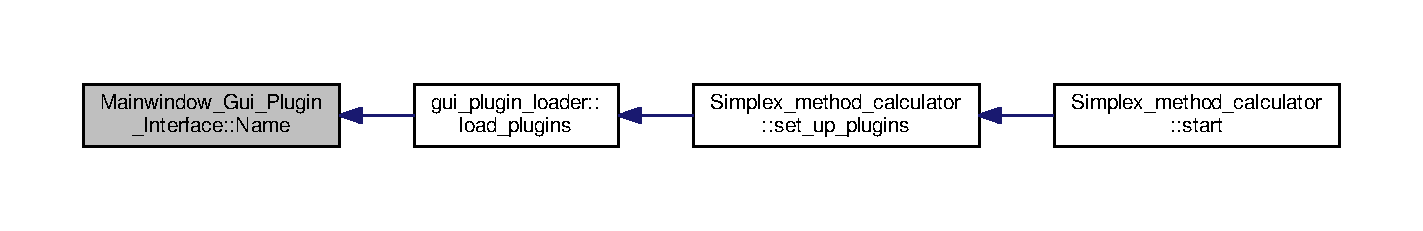
\includegraphics[width=350pt]{classMainwindow__Gui__Plugin__Interface_a5cbc7bb0e3bb477472b91f65e916db8e_icgraph}
\end{center}
\end{figure}
\mbox{\Hypertarget{classMainwindow__Gui__Plugin__Interface_a5cbc7bb0e3bb477472b91f65e916db8e}\label{classMainwindow__Gui__Plugin__Interface_a5cbc7bb0e3bb477472b91f65e916db8e}} 
\index{Mainwindow\+\_\+\+Gui\+\_\+\+Plugin\+\_\+\+Interface@{Mainwindow\+\_\+\+Gui\+\_\+\+Plugin\+\_\+\+Interface}!Name@{Name}}
\index{Name@{Name}!Mainwindow\+\_\+\+Gui\+\_\+\+Plugin\+\_\+\+Interface@{Mainwindow\+\_\+\+Gui\+\_\+\+Plugin\+\_\+\+Interface}}
\subsubsection{\texorpdfstring{Name()}{Name()}\hspace{0.1cm}{\footnotesize\ttfamily [3/3]}}
{\footnotesize\ttfamily virtual Q\+String Mainwindow\+\_\+\+Gui\+\_\+\+Plugin\+\_\+\+Interface\+::\+Name (\begin{DoxyParamCaption}{ }\end{DoxyParamCaption}) const\hspace{0.3cm}{\ttfamily [pure virtual]}}



Implemented in \hyperlink{classMainvindow__gui__plugin_affd8ce27d7e94a2adac287bc8dd835e0}{Mainvindow\+\_\+gui\+\_\+plugin}, and \hyperlink{classMainvindow__gui__plugin__for__fules_abfd45e12e05f78b189c4ad00f7fb6930}{Mainvindow\+\_\+gui\+\_\+plugin\+\_\+for\+\_\+fules}.

\mbox{\Hypertarget{classMainwindow__Gui__Plugin__Interface_ac9422e891b27c71e494d8e48b85fd2dd}\label{classMainwindow__Gui__Plugin__Interface_ac9422e891b27c71e494d8e48b85fd2dd}} 
\index{Mainwindow\+\_\+\+Gui\+\_\+\+Plugin\+\_\+\+Interface@{Mainwindow\+\_\+\+Gui\+\_\+\+Plugin\+\_\+\+Interface}!sor\+\_\+oszlop\+\_\+db@{sor\+\_\+oszlop\+\_\+db}}
\index{sor\+\_\+oszlop\+\_\+db@{sor\+\_\+oszlop\+\_\+db}!Mainwindow\+\_\+\+Gui\+\_\+\+Plugin\+\_\+\+Interface@{Mainwindow\+\_\+\+Gui\+\_\+\+Plugin\+\_\+\+Interface}}
\subsubsection{\texorpdfstring{sor\+\_\+oszlop\+\_\+db}{sor\_oszlop\_db}\hspace{0.1cm}{\footnotesize\ttfamily [1/3]}}
{\footnotesize\ttfamily virtual void Mainwindow\+\_\+\+Gui\+\_\+\+Plugin\+\_\+\+Interface\+::sor\+\_\+oszlop\+\_\+db (\begin{DoxyParamCaption}\item[{int}]{,  }\item[{int}]{ }\end{DoxyParamCaption})\hspace{0.3cm}{\ttfamily [pure virtual]}, {\ttfamily [signal]}}

\mbox{\Hypertarget{classMainwindow__Gui__Plugin__Interface_ac9422e891b27c71e494d8e48b85fd2dd}\label{classMainwindow__Gui__Plugin__Interface_ac9422e891b27c71e494d8e48b85fd2dd}} 
\index{Mainwindow\+\_\+\+Gui\+\_\+\+Plugin\+\_\+\+Interface@{Mainwindow\+\_\+\+Gui\+\_\+\+Plugin\+\_\+\+Interface}!sor\+\_\+oszlop\+\_\+db@{sor\+\_\+oszlop\+\_\+db}}
\index{sor\+\_\+oszlop\+\_\+db@{sor\+\_\+oszlop\+\_\+db}!Mainwindow\+\_\+\+Gui\+\_\+\+Plugin\+\_\+\+Interface@{Mainwindow\+\_\+\+Gui\+\_\+\+Plugin\+\_\+\+Interface}}
\subsubsection{\texorpdfstring{sor\+\_\+oszlop\+\_\+db}{sor\_oszlop\_db}\hspace{0.1cm}{\footnotesize\ttfamily [2/3]}}
{\footnotesize\ttfamily virtual void Mainwindow\+\_\+\+Gui\+\_\+\+Plugin\+\_\+\+Interface\+::sor\+\_\+oszlop\+\_\+db (\begin{DoxyParamCaption}\item[{int}]{,  }\item[{int}]{ }\end{DoxyParamCaption})\hspace{0.3cm}{\ttfamily [pure virtual]}, {\ttfamily [signal]}}

\mbox{\Hypertarget{classMainwindow__Gui__Plugin__Interface_ac9422e891b27c71e494d8e48b85fd2dd}\label{classMainwindow__Gui__Plugin__Interface_ac9422e891b27c71e494d8e48b85fd2dd}} 
\index{Mainwindow\+\_\+\+Gui\+\_\+\+Plugin\+\_\+\+Interface@{Mainwindow\+\_\+\+Gui\+\_\+\+Plugin\+\_\+\+Interface}!sor\+\_\+oszlop\+\_\+db@{sor\+\_\+oszlop\+\_\+db}}
\index{sor\+\_\+oszlop\+\_\+db@{sor\+\_\+oszlop\+\_\+db}!Mainwindow\+\_\+\+Gui\+\_\+\+Plugin\+\_\+\+Interface@{Mainwindow\+\_\+\+Gui\+\_\+\+Plugin\+\_\+\+Interface}}
\subsubsection{\texorpdfstring{sor\+\_\+oszlop\+\_\+db}{sor\_oszlop\_db}\hspace{0.1cm}{\footnotesize\ttfamily [3/3]}}
{\footnotesize\ttfamily virtual void Mainwindow\+\_\+\+Gui\+\_\+\+Plugin\+\_\+\+Interface\+::sor\+\_\+oszlop\+\_\+db (\begin{DoxyParamCaption}\item[{int}]{,  }\item[{int}]{ }\end{DoxyParamCaption})\hspace{0.3cm}{\ttfamily [pure virtual]}, {\ttfamily [signal]}}

\mbox{\Hypertarget{classMainwindow__Gui__Plugin__Interface_aca2e7efeb264c5555dd4ae21bdba009b}\label{classMainwindow__Gui__Plugin__Interface_aca2e7efeb264c5555dd4ae21bdba009b}} 
\index{Mainwindow\+\_\+\+Gui\+\_\+\+Plugin\+\_\+\+Interface@{Mainwindow\+\_\+\+Gui\+\_\+\+Plugin\+\_\+\+Interface}!szamol@{szamol}}
\index{szamol@{szamol}!Mainwindow\+\_\+\+Gui\+\_\+\+Plugin\+\_\+\+Interface@{Mainwindow\+\_\+\+Gui\+\_\+\+Plugin\+\_\+\+Interface}}
\subsubsection{\texorpdfstring{szamol}{szamol}\hspace{0.1cm}{\footnotesize\ttfamily [1/3]}}
{\footnotesize\ttfamily virtual void Mainwindow\+\_\+\+Gui\+\_\+\+Plugin\+\_\+\+Interface\+::szamol (\begin{DoxyParamCaption}{ }\end{DoxyParamCaption})\hspace{0.3cm}{\ttfamily [pure virtual]}, {\ttfamily [signal]}}

\mbox{\Hypertarget{classMainwindow__Gui__Plugin__Interface_aca2e7efeb264c5555dd4ae21bdba009b}\label{classMainwindow__Gui__Plugin__Interface_aca2e7efeb264c5555dd4ae21bdba009b}} 
\index{Mainwindow\+\_\+\+Gui\+\_\+\+Plugin\+\_\+\+Interface@{Mainwindow\+\_\+\+Gui\+\_\+\+Plugin\+\_\+\+Interface}!szamol@{szamol}}
\index{szamol@{szamol}!Mainwindow\+\_\+\+Gui\+\_\+\+Plugin\+\_\+\+Interface@{Mainwindow\+\_\+\+Gui\+\_\+\+Plugin\+\_\+\+Interface}}
\subsubsection{\texorpdfstring{szamol}{szamol}\hspace{0.1cm}{\footnotesize\ttfamily [2/3]}}
{\footnotesize\ttfamily virtual void Mainwindow\+\_\+\+Gui\+\_\+\+Plugin\+\_\+\+Interface\+::szamol (\begin{DoxyParamCaption}{ }\end{DoxyParamCaption})\hspace{0.3cm}{\ttfamily [pure virtual]}, {\ttfamily [signal]}}

\mbox{\Hypertarget{classMainwindow__Gui__Plugin__Interface_aca2e7efeb264c5555dd4ae21bdba009b}\label{classMainwindow__Gui__Plugin__Interface_aca2e7efeb264c5555dd4ae21bdba009b}} 
\index{Mainwindow\+\_\+\+Gui\+\_\+\+Plugin\+\_\+\+Interface@{Mainwindow\+\_\+\+Gui\+\_\+\+Plugin\+\_\+\+Interface}!szamol@{szamol}}
\index{szamol@{szamol}!Mainwindow\+\_\+\+Gui\+\_\+\+Plugin\+\_\+\+Interface@{Mainwindow\+\_\+\+Gui\+\_\+\+Plugin\+\_\+\+Interface}}
\subsubsection{\texorpdfstring{szamol}{szamol}\hspace{0.1cm}{\footnotesize\ttfamily [3/3]}}
{\footnotesize\ttfamily virtual void Mainwindow\+\_\+\+Gui\+\_\+\+Plugin\+\_\+\+Interface\+::szamol (\begin{DoxyParamCaption}{ }\end{DoxyParamCaption})\hspace{0.3cm}{\ttfamily [pure virtual]}, {\ttfamily [signal]}}

\mbox{\Hypertarget{classMainwindow__Gui__Plugin__Interface_a5ef9f7b5d5befab0f74eccefe9313062}\label{classMainwindow__Gui__Plugin__Interface_a5ef9f7b5d5befab0f74eccefe9313062}} 
\index{Mainwindow\+\_\+\+Gui\+\_\+\+Plugin\+\_\+\+Interface@{Mainwindow\+\_\+\+Gui\+\_\+\+Plugin\+\_\+\+Interface}!vegigszamol@{vegigszamol}}
\index{vegigszamol@{vegigszamol}!Mainwindow\+\_\+\+Gui\+\_\+\+Plugin\+\_\+\+Interface@{Mainwindow\+\_\+\+Gui\+\_\+\+Plugin\+\_\+\+Interface}}
\subsubsection{\texorpdfstring{vegigszamol}{vegigszamol}\hspace{0.1cm}{\footnotesize\ttfamily [1/3]}}
{\footnotesize\ttfamily virtual void Mainwindow\+\_\+\+Gui\+\_\+\+Plugin\+\_\+\+Interface\+::vegigszamol (\begin{DoxyParamCaption}\item[{bool}]{vegigszamolando }\end{DoxyParamCaption})\hspace{0.3cm}{\ttfamily [pure virtual]}, {\ttfamily [signal]}}

\mbox{\Hypertarget{classMainwindow__Gui__Plugin__Interface_a5ef9f7b5d5befab0f74eccefe9313062}\label{classMainwindow__Gui__Plugin__Interface_a5ef9f7b5d5befab0f74eccefe9313062}} 
\index{Mainwindow\+\_\+\+Gui\+\_\+\+Plugin\+\_\+\+Interface@{Mainwindow\+\_\+\+Gui\+\_\+\+Plugin\+\_\+\+Interface}!vegigszamol@{vegigszamol}}
\index{vegigszamol@{vegigszamol}!Mainwindow\+\_\+\+Gui\+\_\+\+Plugin\+\_\+\+Interface@{Mainwindow\+\_\+\+Gui\+\_\+\+Plugin\+\_\+\+Interface}}
\subsubsection{\texorpdfstring{vegigszamol}{vegigszamol}\hspace{0.1cm}{\footnotesize\ttfamily [2/3]}}
{\footnotesize\ttfamily virtual void Mainwindow\+\_\+\+Gui\+\_\+\+Plugin\+\_\+\+Interface\+::vegigszamol (\begin{DoxyParamCaption}\item[{bool}]{vegigszamolando }\end{DoxyParamCaption})\hspace{0.3cm}{\ttfamily [pure virtual]}, {\ttfamily [signal]}}

\mbox{\Hypertarget{classMainwindow__Gui__Plugin__Interface_a5ef9f7b5d5befab0f74eccefe9313062}\label{classMainwindow__Gui__Plugin__Interface_a5ef9f7b5d5befab0f74eccefe9313062}} 
\index{Mainwindow\+\_\+\+Gui\+\_\+\+Plugin\+\_\+\+Interface@{Mainwindow\+\_\+\+Gui\+\_\+\+Plugin\+\_\+\+Interface}!vegigszamol@{vegigszamol}}
\index{vegigszamol@{vegigszamol}!Mainwindow\+\_\+\+Gui\+\_\+\+Plugin\+\_\+\+Interface@{Mainwindow\+\_\+\+Gui\+\_\+\+Plugin\+\_\+\+Interface}}
\subsubsection{\texorpdfstring{vegigszamol}{vegigszamol}\hspace{0.1cm}{\footnotesize\ttfamily [3/3]}}
{\footnotesize\ttfamily virtual void Mainwindow\+\_\+\+Gui\+\_\+\+Plugin\+\_\+\+Interface\+::vegigszamol (\begin{DoxyParamCaption}\item[{bool}]{vegigszamolando }\end{DoxyParamCaption})\hspace{0.3cm}{\ttfamily [pure virtual]}, {\ttfamily [signal]}}



The documentation for this class was generated from the following file\+:\begin{DoxyCompactItemize}
\item 
fules/\hyperlink{fules_2mainwindow__gui__plugin__interface_8h}{mainwindow\+\_\+gui\+\_\+plugin\+\_\+interface.\+h}\end{DoxyCompactItemize}

\hypertarget{classNevjegy}{}\section{Nevjegy Class Reference}
\label{classNevjegy}\index{Nevjegy@{Nevjegy}}


{\ttfamily \#include $<$nevjegy.\+h$>$}



Inherits Q\+Dialog.

\subsection*{Public Member Functions}
\begin{DoxyCompactItemize}
\item 
\hyperlink{classNevjegy_abd3f15b023f39e48ef5d79c384bea1d1}{Nevjegy} (Q\+Widget $\ast$parent=nullptr)
\item 
\hyperlink{classNevjegy_a9521f7b858472228b5b8d39438b67432}{$\sim$\+Nevjegy} ()
\end{DoxyCompactItemize}
\subsection*{Private Attributes}
\begin{DoxyCompactItemize}
\item 
Ui\+::\+Nevjegy $\ast$ \hyperlink{classNevjegy_ad971d94faab06f49928fb7f0b844105f}{ui}
\item 
Q\+Pixmap \hyperlink{classNevjegy_a4d025918cbecfe2da5184b98e63501df}{pic1}
\end{DoxyCompactItemize}


\subsection{Detailed Description}


Definition at line 9 of file nevjegy.\+h.



\subsection{Constructor \& Destructor Documentation}
\mbox{\Hypertarget{classNevjegy_abd3f15b023f39e48ef5d79c384bea1d1}\label{classNevjegy_abd3f15b023f39e48ef5d79c384bea1d1}} 
\index{Nevjegy@{Nevjegy}!Nevjegy@{Nevjegy}}
\index{Nevjegy@{Nevjegy}!Nevjegy@{Nevjegy}}
\subsubsection{\texorpdfstring{Nevjegy()}{Nevjegy()}}
{\footnotesize\ttfamily Nevjegy\+::\+Nevjegy (\begin{DoxyParamCaption}\item[{Q\+Widget $\ast$}]{parent = {\ttfamily nullptr} }\end{DoxyParamCaption})\hspace{0.3cm}{\ttfamily [explicit]}}



Definition at line 4 of file nevjegy.\+cpp.

\mbox{\Hypertarget{classNevjegy_a9521f7b858472228b5b8d39438b67432}\label{classNevjegy_a9521f7b858472228b5b8d39438b67432}} 
\index{Nevjegy@{Nevjegy}!````~Nevjegy@{$\sim$\+Nevjegy}}
\index{````~Nevjegy@{$\sim$\+Nevjegy}!Nevjegy@{Nevjegy}}
\subsubsection{\texorpdfstring{$\sim$\+Nevjegy()}{~Nevjegy()}}
{\footnotesize\ttfamily Nevjegy\+::$\sim$\+Nevjegy (\begin{DoxyParamCaption}{ }\end{DoxyParamCaption})}



Definition at line 17 of file nevjegy.\+cpp.



\subsection{Member Data Documentation}
\mbox{\Hypertarget{classNevjegy_a4d025918cbecfe2da5184b98e63501df}\label{classNevjegy_a4d025918cbecfe2da5184b98e63501df}} 
\index{Nevjegy@{Nevjegy}!pic1@{pic1}}
\index{pic1@{pic1}!Nevjegy@{Nevjegy}}
\subsubsection{\texorpdfstring{pic1}{pic1}}
{\footnotesize\ttfamily Q\+Pixmap Nevjegy\+::pic1\hspace{0.3cm}{\ttfamily [private]}}



Definition at line 19 of file nevjegy.\+h.

\mbox{\Hypertarget{classNevjegy_ad971d94faab06f49928fb7f0b844105f}\label{classNevjegy_ad971d94faab06f49928fb7f0b844105f}} 
\index{Nevjegy@{Nevjegy}!ui@{ui}}
\index{ui@{ui}!Nevjegy@{Nevjegy}}
\subsubsection{\texorpdfstring{ui}{ui}}
{\footnotesize\ttfamily Ui\+::\+Nevjegy$\ast$ Nevjegy\+::ui\hspace{0.3cm}{\ttfamily [private]}}



Definition at line 18 of file nevjegy.\+h.



The documentation for this class was generated from the following files\+:\begin{DoxyCompactItemize}
\item 
simplex\+\_\+app/\hyperlink{nevjegy_8h}{nevjegy.\+h}\item 
simplex\+\_\+app/\hyperlink{nevjegy_8cpp}{nevjegy.\+cpp}\end{DoxyCompactItemize}

\hypertarget{classNon__numeric__Delegate}{}\section{Non\+\_\+numeric\+\_\+\+Delegate Class Reference}
\label{classNon__numeric__Delegate}\index{Non\+\_\+numeric\+\_\+\+Delegate@{Non\+\_\+numeric\+\_\+\+Delegate}}


{\ttfamily \#include $<$non\+\_\+numeric\+\_\+delegate.\+h$>$}



Inherits Q\+Item\+Delegate.

\subsection*{Public Member Functions}
\begin{DoxyCompactItemize}
\item 
\hyperlink{classNon__numeric__Delegate_ae2fb0931922c20c796bfa85921dc880f}{Non\+\_\+numeric\+\_\+\+Delegate} (Q\+Object $\ast$parent=0)
\item 
Q\+Widget $\ast$ \hyperlink{classNon__numeric__Delegate_a073f05382a36c178750c522fe82dda8d}{create\+Editor} (Q\+Widget $\ast$parent, const Q\+Style\+Option\+View\+Item \&option, const Q\+Model\+Index \&index) const
\item 
void \hyperlink{classNon__numeric__Delegate_a8d3048dc7212637a785670aa5f5c9043}{set\+Editor\+Data} (Q\+Widget $\ast$editor, const Q\+Model\+Index \&index) const
\item 
void \hyperlink{classNon__numeric__Delegate_a517cb55e57c8a6c86eee133141f7b6cb}{set\+Model\+Data} (Q\+Widget $\ast$editor, Q\+Abstract\+Item\+Model $\ast$model, const Q\+Model\+Index \&index) const
\item 
void \hyperlink{classNon__numeric__Delegate_ac5d634e38c5445a0c9220008840488b9}{update\+Editor\+Geometry} (Q\+Widget $\ast$editor, const Q\+Style\+Option\+View\+Item \&option, const Q\+Model\+Index \&index) const
\end{DoxyCompactItemize}


\subsection{Detailed Description}


Definition at line 13 of file non\+\_\+numeric\+\_\+delegate.\+h.



\subsection{Constructor \& Destructor Documentation}
\mbox{\Hypertarget{classNon__numeric__Delegate_ae2fb0931922c20c796bfa85921dc880f}\label{classNon__numeric__Delegate_ae2fb0931922c20c796bfa85921dc880f}} 
\index{Non\+\_\+numeric\+\_\+\+Delegate@{Non\+\_\+numeric\+\_\+\+Delegate}!Non\+\_\+numeric\+\_\+\+Delegate@{Non\+\_\+numeric\+\_\+\+Delegate}}
\index{Non\+\_\+numeric\+\_\+\+Delegate@{Non\+\_\+numeric\+\_\+\+Delegate}!Non\+\_\+numeric\+\_\+\+Delegate@{Non\+\_\+numeric\+\_\+\+Delegate}}
\subsubsection{\texorpdfstring{Non\+\_\+numeric\+\_\+\+Delegate()}{Non\_numeric\_Delegate()}}
{\footnotesize\ttfamily Non\+\_\+numeric\+\_\+\+Delegate\+::\+Non\+\_\+numeric\+\_\+\+Delegate (\begin{DoxyParamCaption}\item[{Q\+Object $\ast$}]{parent = {\ttfamily 0} }\end{DoxyParamCaption})}



Definition at line 6 of file non\+\_\+numeric\+\_\+delegate.\+cpp.



\subsection{Member Function Documentation}
\mbox{\Hypertarget{classNon__numeric__Delegate_a073f05382a36c178750c522fe82dda8d}\label{classNon__numeric__Delegate_a073f05382a36c178750c522fe82dda8d}} 
\index{Non\+\_\+numeric\+\_\+\+Delegate@{Non\+\_\+numeric\+\_\+\+Delegate}!create\+Editor@{create\+Editor}}
\index{create\+Editor@{create\+Editor}!Non\+\_\+numeric\+\_\+\+Delegate@{Non\+\_\+numeric\+\_\+\+Delegate}}
\subsubsection{\texorpdfstring{create\+Editor()}{createEditor()}}
{\footnotesize\ttfamily Q\+Widget $\ast$ Non\+\_\+numeric\+\_\+\+Delegate\+::create\+Editor (\begin{DoxyParamCaption}\item[{Q\+Widget $\ast$}]{parent,  }\item[{const Q\+Style\+Option\+View\+Item \&}]{option,  }\item[{const Q\+Model\+Index \&}]{index }\end{DoxyParamCaption}) const}



Definition at line 11 of file non\+\_\+numeric\+\_\+delegate.\+cpp.

\mbox{\Hypertarget{classNon__numeric__Delegate_a8d3048dc7212637a785670aa5f5c9043}\label{classNon__numeric__Delegate_a8d3048dc7212637a785670aa5f5c9043}} 
\index{Non\+\_\+numeric\+\_\+\+Delegate@{Non\+\_\+numeric\+\_\+\+Delegate}!set\+Editor\+Data@{set\+Editor\+Data}}
\index{set\+Editor\+Data@{set\+Editor\+Data}!Non\+\_\+numeric\+\_\+\+Delegate@{Non\+\_\+numeric\+\_\+\+Delegate}}
\subsubsection{\texorpdfstring{set\+Editor\+Data()}{setEditorData()}}
{\footnotesize\ttfamily void Non\+\_\+numeric\+\_\+\+Delegate\+::set\+Editor\+Data (\begin{DoxyParamCaption}\item[{Q\+Widget $\ast$}]{editor,  }\item[{const Q\+Model\+Index \&}]{index }\end{DoxyParamCaption}) const}



Definition at line 30 of file non\+\_\+numeric\+\_\+delegate.\+cpp.

\mbox{\Hypertarget{classNon__numeric__Delegate_a517cb55e57c8a6c86eee133141f7b6cb}\label{classNon__numeric__Delegate_a517cb55e57c8a6c86eee133141f7b6cb}} 
\index{Non\+\_\+numeric\+\_\+\+Delegate@{Non\+\_\+numeric\+\_\+\+Delegate}!set\+Model\+Data@{set\+Model\+Data}}
\index{set\+Model\+Data@{set\+Model\+Data}!Non\+\_\+numeric\+\_\+\+Delegate@{Non\+\_\+numeric\+\_\+\+Delegate}}
\subsubsection{\texorpdfstring{set\+Model\+Data()}{setModelData()}}
{\footnotesize\ttfamily void Non\+\_\+numeric\+\_\+\+Delegate\+::set\+Model\+Data (\begin{DoxyParamCaption}\item[{Q\+Widget $\ast$}]{editor,  }\item[{Q\+Abstract\+Item\+Model $\ast$}]{model,  }\item[{const Q\+Model\+Index \&}]{index }\end{DoxyParamCaption}) const}



Definition at line 36 of file non\+\_\+numeric\+\_\+delegate.\+cpp.

\mbox{\Hypertarget{classNon__numeric__Delegate_ac5d634e38c5445a0c9220008840488b9}\label{classNon__numeric__Delegate_ac5d634e38c5445a0c9220008840488b9}} 
\index{Non\+\_\+numeric\+\_\+\+Delegate@{Non\+\_\+numeric\+\_\+\+Delegate}!update\+Editor\+Geometry@{update\+Editor\+Geometry}}
\index{update\+Editor\+Geometry@{update\+Editor\+Geometry}!Non\+\_\+numeric\+\_\+\+Delegate@{Non\+\_\+numeric\+\_\+\+Delegate}}
\subsubsection{\texorpdfstring{update\+Editor\+Geometry()}{updateEditorGeometry()}}
{\footnotesize\ttfamily void Non\+\_\+numeric\+\_\+\+Delegate\+::update\+Editor\+Geometry (\begin{DoxyParamCaption}\item[{Q\+Widget $\ast$}]{editor,  }\item[{const Q\+Style\+Option\+View\+Item \&}]{option,  }\item[{const Q\+Model\+Index \&}]{index }\end{DoxyParamCaption}) const}



Definition at line 44 of file non\+\_\+numeric\+\_\+delegate.\+cpp.



The documentation for this class was generated from the following files\+:\begin{DoxyCompactItemize}
\item 
simplex\+\_\+app/\hyperlink{non__numeric__delegate_8h}{non\+\_\+numeric\+\_\+delegate.\+h}\item 
simplex\+\_\+app/\hyperlink{non__numeric__delegate_8cpp}{non\+\_\+numeric\+\_\+delegate.\+cpp}\end{DoxyCompactItemize}

\hypertarget{classNon__numeric__Delegate__in__fules}{}\section{Non\+\_\+numeric\+\_\+\+Delegate\+\_\+in\+\_\+fules Class Reference}
\label{classNon__numeric__Delegate__in__fules}\index{Non\+\_\+numeric\+\_\+\+Delegate\+\_\+in\+\_\+fules@{Non\+\_\+numeric\+\_\+\+Delegate\+\_\+in\+\_\+fules}}


{\ttfamily \#include $<$non\+\_\+numeric\+\_\+delegate\+\_\+in\+\_\+fules.\+h$>$}



Inherits Q\+Item\+Delegate.

\subsection*{Public Member Functions}
\begin{DoxyCompactItemize}
\item 
\hyperlink{classNon__numeric__Delegate__in__fules_a67d03bdb8f3797c80f8987c429e5d420}{Non\+\_\+numeric\+\_\+\+Delegate\+\_\+in\+\_\+fules} (Q\+Object $\ast$parent=nullptr)
\item 
Q\+Widget $\ast$ \hyperlink{classNon__numeric__Delegate__in__fules_a5deaa64416800b2b76bddc65f509e51b}{create\+Editor} (Q\+Widget $\ast$parent, const Q\+Style\+Option\+View\+Item \&option, const Q\+Model\+Index \&index) const
\item 
void \hyperlink{classNon__numeric__Delegate__in__fules_a164816b371172eb34b15233572ca32d5}{set\+Editor\+Data} (Q\+Widget $\ast$editor, const Q\+Model\+Index \&index) const
\item 
void \hyperlink{classNon__numeric__Delegate__in__fules_a31b9113d3edd7aa449f712b449ba0b08}{set\+Model\+Data} (Q\+Widget $\ast$editor, Q\+Abstract\+Item\+Model $\ast$model, const Q\+Model\+Index \&index) const
\item 
void \hyperlink{classNon__numeric__Delegate__in__fules_ac13c2aff394211c408ff1e7d504ee717}{update\+Editor\+Geometry} (Q\+Widget $\ast$editor, const Q\+Style\+Option\+View\+Item \&option, const Q\+Model\+Index \&index) const
\end{DoxyCompactItemize}


\subsection{Detailed Description}


Definition at line 13 of file non\+\_\+numeric\+\_\+delegate\+\_\+in\+\_\+fules.\+h.



\subsection{Constructor \& Destructor Documentation}
\mbox{\Hypertarget{classNon__numeric__Delegate__in__fules_a67d03bdb8f3797c80f8987c429e5d420}\label{classNon__numeric__Delegate__in__fules_a67d03bdb8f3797c80f8987c429e5d420}} 
\index{Non\+\_\+numeric\+\_\+\+Delegate\+\_\+in\+\_\+fules@{Non\+\_\+numeric\+\_\+\+Delegate\+\_\+in\+\_\+fules}!Non\+\_\+numeric\+\_\+\+Delegate\+\_\+in\+\_\+fules@{Non\+\_\+numeric\+\_\+\+Delegate\+\_\+in\+\_\+fules}}
\index{Non\+\_\+numeric\+\_\+\+Delegate\+\_\+in\+\_\+fules@{Non\+\_\+numeric\+\_\+\+Delegate\+\_\+in\+\_\+fules}!Non\+\_\+numeric\+\_\+\+Delegate\+\_\+in\+\_\+fules@{Non\+\_\+numeric\+\_\+\+Delegate\+\_\+in\+\_\+fules}}
\subsubsection{\texorpdfstring{Non\+\_\+numeric\+\_\+\+Delegate\+\_\+in\+\_\+fules()}{Non\_numeric\_Delegate\_in\_fules()}}
{\footnotesize\ttfamily Non\+\_\+numeric\+\_\+\+Delegate\+\_\+in\+\_\+fules\+::\+Non\+\_\+numeric\+\_\+\+Delegate\+\_\+in\+\_\+fules (\begin{DoxyParamCaption}\item[{Q\+Object $\ast$}]{parent = {\ttfamily nullptr} }\end{DoxyParamCaption})}



Definition at line 6 of file non\+\_\+numeric\+\_\+delegate\+\_\+in\+\_\+fules.\+cpp.



\subsection{Member Function Documentation}
\mbox{\Hypertarget{classNon__numeric__Delegate__in__fules_a5deaa64416800b2b76bddc65f509e51b}\label{classNon__numeric__Delegate__in__fules_a5deaa64416800b2b76bddc65f509e51b}} 
\index{Non\+\_\+numeric\+\_\+\+Delegate\+\_\+in\+\_\+fules@{Non\+\_\+numeric\+\_\+\+Delegate\+\_\+in\+\_\+fules}!create\+Editor@{create\+Editor}}
\index{create\+Editor@{create\+Editor}!Non\+\_\+numeric\+\_\+\+Delegate\+\_\+in\+\_\+fules@{Non\+\_\+numeric\+\_\+\+Delegate\+\_\+in\+\_\+fules}}
\subsubsection{\texorpdfstring{create\+Editor()}{createEditor()}}
{\footnotesize\ttfamily Q\+Widget $\ast$ Non\+\_\+numeric\+\_\+\+Delegate\+\_\+in\+\_\+fules\+::create\+Editor (\begin{DoxyParamCaption}\item[{Q\+Widget $\ast$}]{parent,  }\item[{const Q\+Style\+Option\+View\+Item \&}]{option,  }\item[{const Q\+Model\+Index \&}]{index }\end{DoxyParamCaption}) const}



Definition at line 11 of file non\+\_\+numeric\+\_\+delegate\+\_\+in\+\_\+fules.\+cpp.

\mbox{\Hypertarget{classNon__numeric__Delegate__in__fules_a164816b371172eb34b15233572ca32d5}\label{classNon__numeric__Delegate__in__fules_a164816b371172eb34b15233572ca32d5}} 
\index{Non\+\_\+numeric\+\_\+\+Delegate\+\_\+in\+\_\+fules@{Non\+\_\+numeric\+\_\+\+Delegate\+\_\+in\+\_\+fules}!set\+Editor\+Data@{set\+Editor\+Data}}
\index{set\+Editor\+Data@{set\+Editor\+Data}!Non\+\_\+numeric\+\_\+\+Delegate\+\_\+in\+\_\+fules@{Non\+\_\+numeric\+\_\+\+Delegate\+\_\+in\+\_\+fules}}
\subsubsection{\texorpdfstring{set\+Editor\+Data()}{setEditorData()}}
{\footnotesize\ttfamily void Non\+\_\+numeric\+\_\+\+Delegate\+\_\+in\+\_\+fules\+::set\+Editor\+Data (\begin{DoxyParamCaption}\item[{Q\+Widget $\ast$}]{editor,  }\item[{const Q\+Model\+Index \&}]{index }\end{DoxyParamCaption}) const}



Definition at line 30 of file non\+\_\+numeric\+\_\+delegate\+\_\+in\+\_\+fules.\+cpp.

\mbox{\Hypertarget{classNon__numeric__Delegate__in__fules_a31b9113d3edd7aa449f712b449ba0b08}\label{classNon__numeric__Delegate__in__fules_a31b9113d3edd7aa449f712b449ba0b08}} 
\index{Non\+\_\+numeric\+\_\+\+Delegate\+\_\+in\+\_\+fules@{Non\+\_\+numeric\+\_\+\+Delegate\+\_\+in\+\_\+fules}!set\+Model\+Data@{set\+Model\+Data}}
\index{set\+Model\+Data@{set\+Model\+Data}!Non\+\_\+numeric\+\_\+\+Delegate\+\_\+in\+\_\+fules@{Non\+\_\+numeric\+\_\+\+Delegate\+\_\+in\+\_\+fules}}
\subsubsection{\texorpdfstring{set\+Model\+Data()}{setModelData()}}
{\footnotesize\ttfamily void Non\+\_\+numeric\+\_\+\+Delegate\+\_\+in\+\_\+fules\+::set\+Model\+Data (\begin{DoxyParamCaption}\item[{Q\+Widget $\ast$}]{editor,  }\item[{Q\+Abstract\+Item\+Model $\ast$}]{model,  }\item[{const Q\+Model\+Index \&}]{index }\end{DoxyParamCaption}) const}



Definition at line 36 of file non\+\_\+numeric\+\_\+delegate\+\_\+in\+\_\+fules.\+cpp.

\mbox{\Hypertarget{classNon__numeric__Delegate__in__fules_ac13c2aff394211c408ff1e7d504ee717}\label{classNon__numeric__Delegate__in__fules_ac13c2aff394211c408ff1e7d504ee717}} 
\index{Non\+\_\+numeric\+\_\+\+Delegate\+\_\+in\+\_\+fules@{Non\+\_\+numeric\+\_\+\+Delegate\+\_\+in\+\_\+fules}!update\+Editor\+Geometry@{update\+Editor\+Geometry}}
\index{update\+Editor\+Geometry@{update\+Editor\+Geometry}!Non\+\_\+numeric\+\_\+\+Delegate\+\_\+in\+\_\+fules@{Non\+\_\+numeric\+\_\+\+Delegate\+\_\+in\+\_\+fules}}
\subsubsection{\texorpdfstring{update\+Editor\+Geometry()}{updateEditorGeometry()}}
{\footnotesize\ttfamily void Non\+\_\+numeric\+\_\+\+Delegate\+\_\+in\+\_\+fules\+::update\+Editor\+Geometry (\begin{DoxyParamCaption}\item[{Q\+Widget $\ast$}]{editor,  }\item[{const Q\+Style\+Option\+View\+Item \&}]{option,  }\item[{const Q\+Model\+Index \&}]{index }\end{DoxyParamCaption}) const}



Definition at line 44 of file non\+\_\+numeric\+\_\+delegate\+\_\+in\+\_\+fules.\+cpp.



The documentation for this class was generated from the following files\+:\begin{DoxyCompactItemize}
\item 
fules/\hyperlink{non__numeric__delegate__in__fules_8h}{non\+\_\+numeric\+\_\+delegate\+\_\+in\+\_\+fules.\+h}\item 
fules/\hyperlink{non__numeric__delegate__in__fules_8cpp}{non\+\_\+numeric\+\_\+delegate\+\_\+in\+\_\+fules.\+cpp}\end{DoxyCompactItemize}

\hypertarget{classPicture__Load__Plugin__Interface}{}\section{Picture\+\_\+\+Load\+\_\+\+Plugin\+\_\+\+Interface Class Reference}
\label{classPicture__Load__Plugin__Interface}\index{Picture\+\_\+\+Load\+\_\+\+Plugin\+\_\+\+Interface@{Picture\+\_\+\+Load\+\_\+\+Plugin\+\_\+\+Interface}}


{\ttfamily \#include $<$picture\+\_\+load\+\_\+plugin\+\_\+interface.\+h$>$}



Inheritance diagram for Picture\+\_\+\+Load\+\_\+\+Plugin\+\_\+\+Interface\+:\nopagebreak
\begin{figure}[H]
\begin{center}
\leavevmode
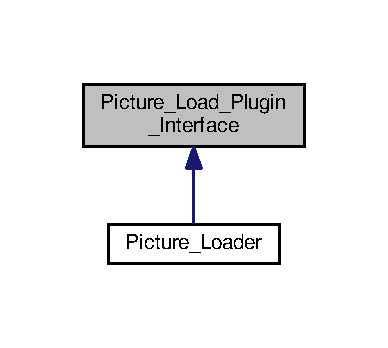
\includegraphics[width=186pt]{classPicture__Load__Plugin__Interface__inherit__graph}
\end{center}
\end{figure}
\subsection*{Public Member Functions}
\begin{DoxyCompactItemize}
\item 
virtual void \hyperlink{classPicture__Load__Plugin__Interface_a2d90e62b277854046ebcdac8ffadf0d5}{show\+\_\+picture} (Q\+Main\+Window $\ast$w)=0
\item 
virtual Q\+String \hyperlink{classPicture__Load__Plugin__Interface_a7cb4c7354f06bc7408ce1072e46db030}{Name} () const =0
\item 
virtual void \hyperlink{classPicture__Load__Plugin__Interface_a2d90e62b277854046ebcdac8ffadf0d5}{show\+\_\+picture} (Q\+Main\+Window $\ast$w)=0
\item 
virtual Q\+String \hyperlink{classPicture__Load__Plugin__Interface_a7cb4c7354f06bc7408ce1072e46db030}{Name} () const =0
\end{DoxyCompactItemize}


\subsection{Detailed Description}


Definition at line 6 of file picture\+\_\+load\+\_\+plugin\+\_\+interface.\+h.



\subsection{Member Function Documentation}
\mbox{\Hypertarget{classPicture__Load__Plugin__Interface_a7cb4c7354f06bc7408ce1072e46db030}\label{classPicture__Load__Plugin__Interface_a7cb4c7354f06bc7408ce1072e46db030}} 
\index{Picture\+\_\+\+Load\+\_\+\+Plugin\+\_\+\+Interface@{Picture\+\_\+\+Load\+\_\+\+Plugin\+\_\+\+Interface}!Name@{Name}}
\index{Name@{Name}!Picture\+\_\+\+Load\+\_\+\+Plugin\+\_\+\+Interface@{Picture\+\_\+\+Load\+\_\+\+Plugin\+\_\+\+Interface}}
\subsubsection{\texorpdfstring{Name()}{Name()}\hspace{0.1cm}{\footnotesize\ttfamily [1/2]}}
{\footnotesize\ttfamily virtual Q\+String Picture\+\_\+\+Load\+\_\+\+Plugin\+\_\+\+Interface\+::\+Name (\begin{DoxyParamCaption}{ }\end{DoxyParamCaption}) const\hspace{0.3cm}{\ttfamily [pure virtual]}}



Implemented in \hyperlink{classPicture__Loader_a043165c946b7bf29dea761463b8cb5fa}{Picture\+\_\+\+Loader}.

\mbox{\Hypertarget{classPicture__Load__Plugin__Interface_a7cb4c7354f06bc7408ce1072e46db030}\label{classPicture__Load__Plugin__Interface_a7cb4c7354f06bc7408ce1072e46db030}} 
\index{Picture\+\_\+\+Load\+\_\+\+Plugin\+\_\+\+Interface@{Picture\+\_\+\+Load\+\_\+\+Plugin\+\_\+\+Interface}!Name@{Name}}
\index{Name@{Name}!Picture\+\_\+\+Load\+\_\+\+Plugin\+\_\+\+Interface@{Picture\+\_\+\+Load\+\_\+\+Plugin\+\_\+\+Interface}}
\subsubsection{\texorpdfstring{Name()}{Name()}\hspace{0.1cm}{\footnotesize\ttfamily [2/2]}}
{\footnotesize\ttfamily virtual Q\+String Picture\+\_\+\+Load\+\_\+\+Plugin\+\_\+\+Interface\+::\+Name (\begin{DoxyParamCaption}{ }\end{DoxyParamCaption}) const\hspace{0.3cm}{\ttfamily [pure virtual]}}



Implemented in \hyperlink{classPicture__Loader_a043165c946b7bf29dea761463b8cb5fa}{Picture\+\_\+\+Loader}.

Here is the caller graph for this function\+:\nopagebreak
\begin{figure}[H]
\begin{center}
\leavevmode
\includegraphics[width=350pt]{classPicture__Load__Plugin__Interface_a7cb4c7354f06bc7408ce1072e46db030_icgraph}
\end{center}
\end{figure}
\mbox{\Hypertarget{classPicture__Load__Plugin__Interface_a2d90e62b277854046ebcdac8ffadf0d5}\label{classPicture__Load__Plugin__Interface_a2d90e62b277854046ebcdac8ffadf0d5}} 
\index{Picture\+\_\+\+Load\+\_\+\+Plugin\+\_\+\+Interface@{Picture\+\_\+\+Load\+\_\+\+Plugin\+\_\+\+Interface}!show\+\_\+picture@{show\+\_\+picture}}
\index{show\+\_\+picture@{show\+\_\+picture}!Picture\+\_\+\+Load\+\_\+\+Plugin\+\_\+\+Interface@{Picture\+\_\+\+Load\+\_\+\+Plugin\+\_\+\+Interface}}
\subsubsection{\texorpdfstring{show\+\_\+picture()}{show\_picture()}\hspace{0.1cm}{\footnotesize\ttfamily [1/2]}}
{\footnotesize\ttfamily virtual void Picture\+\_\+\+Load\+\_\+\+Plugin\+\_\+\+Interface\+::show\+\_\+picture (\begin{DoxyParamCaption}\item[{Q\+Main\+Window $\ast$}]{w }\end{DoxyParamCaption})\hspace{0.3cm}{\ttfamily [pure virtual]}}



Implemented in \hyperlink{classPicture__Loader_af4127aaea7066112b2368adda46a82b0}{Picture\+\_\+\+Loader}.

\mbox{\Hypertarget{classPicture__Load__Plugin__Interface_a2d90e62b277854046ebcdac8ffadf0d5}\label{classPicture__Load__Plugin__Interface_a2d90e62b277854046ebcdac8ffadf0d5}} 
\index{Picture\+\_\+\+Load\+\_\+\+Plugin\+\_\+\+Interface@{Picture\+\_\+\+Load\+\_\+\+Plugin\+\_\+\+Interface}!show\+\_\+picture@{show\+\_\+picture}}
\index{show\+\_\+picture@{show\+\_\+picture}!Picture\+\_\+\+Load\+\_\+\+Plugin\+\_\+\+Interface@{Picture\+\_\+\+Load\+\_\+\+Plugin\+\_\+\+Interface}}
\subsubsection{\texorpdfstring{show\+\_\+picture()}{show\_picture()}\hspace{0.1cm}{\footnotesize\ttfamily [2/2]}}
{\footnotesize\ttfamily virtual void Picture\+\_\+\+Load\+\_\+\+Plugin\+\_\+\+Interface\+::show\+\_\+picture (\begin{DoxyParamCaption}\item[{Q\+Main\+Window $\ast$}]{w }\end{DoxyParamCaption})\hspace{0.3cm}{\ttfamily [pure virtual]}}



Implemented in \hyperlink{classPicture__Loader_af4127aaea7066112b2368adda46a82b0}{Picture\+\_\+\+Loader}.

Here is the caller graph for this function\+:\nopagebreak
\begin{figure}[H]
\begin{center}
\leavevmode
\includegraphics[width=350pt]{classPicture__Load__Plugin__Interface_a2d90e62b277854046ebcdac8ffadf0d5_icgraph}
\end{center}
\end{figure}


The documentation for this class was generated from the following file\+:\begin{DoxyCompactItemize}
\item 
picture\+\_\+loader/\hyperlink{picture__loader_2picture__load__plugin__interface_8h}{picture\+\_\+load\+\_\+plugin\+\_\+interface.\+h}\end{DoxyCompactItemize}

\hypertarget{classpicture__load__plugin__loader}{}\section{picture\+\_\+load\+\_\+plugin\+\_\+loader Class Reference}
\label{classpicture__load__plugin__loader}\index{picture\+\_\+load\+\_\+plugin\+\_\+loader@{picture\+\_\+load\+\_\+plugin\+\_\+loader}}


{\ttfamily \#include $<$picture\+\_\+load\+\_\+plugin\+\_\+loader.\+h$>$}



Inherits Q\+Object.



Collaboration diagram for picture\+\_\+load\+\_\+plugin\+\_\+loader\+:\nopagebreak
\begin{figure}[H]
\begin{center}
\leavevmode
\includegraphics[width=193pt]{classpicture__load__plugin__loader__coll__graph}
\end{center}
\end{figure}
\subsection*{Public Slots}
\begin{DoxyCompactItemize}
\item 
void \hyperlink{classpicture__load__plugin__loader_a7e8827db78dabf7872b30305e1f29af0}{trigger\+\_\+plugin} (Q\+Action $\ast$menu\+\_\+action)
\end{DoxyCompactItemize}
\subsection*{Public Member Functions}
\begin{DoxyCompactItemize}
\item 
\hyperlink{classpicture__load__plugin__loader_ac548a57f4e400bc5612428a752a1d59e}{picture\+\_\+load\+\_\+plugin\+\_\+loader} (Q\+Object $\ast$parent=nullptr, \hyperlink{classMainWindow}{Main\+Window} $\ast$w=nullptr)
\item 
void \hyperlink{classpicture__load__plugin__loader_a0e59be47c219103db204896cb89f0720}{load\+\_\+plugins} (Q\+Dir root\+\_\+dir)
\end{DoxyCompactItemize}
\subsection*{Private Attributes}
\begin{DoxyCompactItemize}
\item 
Q\+Object $\ast$ \hyperlink{classpicture__load__plugin__loader_a5d0e09fbe0b7b061a785216ee57b5d3b}{parent\+\_\+}
\item 
\hyperlink{classMainWindow}{Main\+Window} $\ast$ \hyperlink{classpicture__load__plugin__loader_a6a6c98c4ff9b1506b82a6a87e2b2103b}{main\+\_\+window}
\end{DoxyCompactItemize}


\subsection{Detailed Description}


Definition at line 10 of file picture\+\_\+load\+\_\+plugin\+\_\+loader.\+h.



\subsection{Constructor \& Destructor Documentation}
\mbox{\Hypertarget{classpicture__load__plugin__loader_ac548a57f4e400bc5612428a752a1d59e}\label{classpicture__load__plugin__loader_ac548a57f4e400bc5612428a752a1d59e}} 
\index{picture\+\_\+load\+\_\+plugin\+\_\+loader@{picture\+\_\+load\+\_\+plugin\+\_\+loader}!picture\+\_\+load\+\_\+plugin\+\_\+loader@{picture\+\_\+load\+\_\+plugin\+\_\+loader}}
\index{picture\+\_\+load\+\_\+plugin\+\_\+loader@{picture\+\_\+load\+\_\+plugin\+\_\+loader}!picture\+\_\+load\+\_\+plugin\+\_\+loader@{picture\+\_\+load\+\_\+plugin\+\_\+loader}}
\subsubsection{\texorpdfstring{picture\+\_\+load\+\_\+plugin\+\_\+loader()}{picture\_load\_plugin\_loader()}}
{\footnotesize\ttfamily picture\+\_\+load\+\_\+plugin\+\_\+loader\+::picture\+\_\+load\+\_\+plugin\+\_\+loader (\begin{DoxyParamCaption}\item[{Q\+Object $\ast$}]{parent = {\ttfamily nullptr},  }\item[{\hyperlink{classMainWindow}{Main\+Window} $\ast$}]{w = {\ttfamily nullptr} }\end{DoxyParamCaption})\hspace{0.3cm}{\ttfamily [explicit]}}



Definition at line 3 of file picture\+\_\+load\+\_\+plugin\+\_\+loader.\+cpp.



\subsection{Member Function Documentation}
\mbox{\Hypertarget{classpicture__load__plugin__loader_a0e59be47c219103db204896cb89f0720}\label{classpicture__load__plugin__loader_a0e59be47c219103db204896cb89f0720}} 
\index{picture\+\_\+load\+\_\+plugin\+\_\+loader@{picture\+\_\+load\+\_\+plugin\+\_\+loader}!load\+\_\+plugins@{load\+\_\+plugins}}
\index{load\+\_\+plugins@{load\+\_\+plugins}!picture\+\_\+load\+\_\+plugin\+\_\+loader@{picture\+\_\+load\+\_\+plugin\+\_\+loader}}
\subsubsection{\texorpdfstring{load\+\_\+plugins()}{load\_plugins()}}
{\footnotesize\ttfamily void picture\+\_\+load\+\_\+plugin\+\_\+loader\+::load\+\_\+plugins (\begin{DoxyParamCaption}\item[{Q\+Dir}]{root\+\_\+dir }\end{DoxyParamCaption})}



Definition at line 8 of file picture\+\_\+load\+\_\+plugin\+\_\+loader.\+cpp.

Here is the call graph for this function\+:\nopagebreak
\begin{figure}[H]
\begin{center}
\leavevmode
\includegraphics[width=350pt]{classpicture__load__plugin__loader_a0e59be47c219103db204896cb89f0720_cgraph}
\end{center}
\end{figure}
Here is the caller graph for this function\+:\nopagebreak
\begin{figure}[H]
\begin{center}
\leavevmode
\includegraphics[width=350pt]{classpicture__load__plugin__loader_a0e59be47c219103db204896cb89f0720_icgraph}
\end{center}
\end{figure}
\mbox{\Hypertarget{classpicture__load__plugin__loader_a7e8827db78dabf7872b30305e1f29af0}\label{classpicture__load__plugin__loader_a7e8827db78dabf7872b30305e1f29af0}} 
\index{picture\+\_\+load\+\_\+plugin\+\_\+loader@{picture\+\_\+load\+\_\+plugin\+\_\+loader}!trigger\+\_\+plugin@{trigger\+\_\+plugin}}
\index{trigger\+\_\+plugin@{trigger\+\_\+plugin}!picture\+\_\+load\+\_\+plugin\+\_\+loader@{picture\+\_\+load\+\_\+plugin\+\_\+loader}}
\subsubsection{\texorpdfstring{trigger\+\_\+plugin}{trigger\_plugin}}
{\footnotesize\ttfamily void picture\+\_\+load\+\_\+plugin\+\_\+loader\+::trigger\+\_\+plugin (\begin{DoxyParamCaption}\item[{Q\+Action $\ast$}]{menu\+\_\+action }\end{DoxyParamCaption})\hspace{0.3cm}{\ttfamily [slot]}}



Definition at line 32 of file picture\+\_\+load\+\_\+plugin\+\_\+loader.\+cpp.

Here is the call graph for this function\+:\nopagebreak
\begin{figure}[H]
\begin{center}
\leavevmode
\includegraphics[width=350pt]{classpicture__load__plugin__loader_a7e8827db78dabf7872b30305e1f29af0_cgraph}
\end{center}
\end{figure}
Here is the caller graph for this function\+:\nopagebreak
\begin{figure}[H]
\begin{center}
\leavevmode
\includegraphics[width=350pt]{classpicture__load__plugin__loader_a7e8827db78dabf7872b30305e1f29af0_icgraph}
\end{center}
\end{figure}


\subsection{Member Data Documentation}
\mbox{\Hypertarget{classpicture__load__plugin__loader_a6a6c98c4ff9b1506b82a6a87e2b2103b}\label{classpicture__load__plugin__loader_a6a6c98c4ff9b1506b82a6a87e2b2103b}} 
\index{picture\+\_\+load\+\_\+plugin\+\_\+loader@{picture\+\_\+load\+\_\+plugin\+\_\+loader}!main\+\_\+window@{main\+\_\+window}}
\index{main\+\_\+window@{main\+\_\+window}!picture\+\_\+load\+\_\+plugin\+\_\+loader@{picture\+\_\+load\+\_\+plugin\+\_\+loader}}
\subsubsection{\texorpdfstring{main\+\_\+window}{main\_window}}
{\footnotesize\ttfamily \hyperlink{classMainWindow}{Main\+Window}$\ast$ picture\+\_\+load\+\_\+plugin\+\_\+loader\+::main\+\_\+window\hspace{0.3cm}{\ttfamily [private]}}



Definition at line 23 of file picture\+\_\+load\+\_\+plugin\+\_\+loader.\+h.

\mbox{\Hypertarget{classpicture__load__plugin__loader_a5d0e09fbe0b7b061a785216ee57b5d3b}\label{classpicture__load__plugin__loader_a5d0e09fbe0b7b061a785216ee57b5d3b}} 
\index{picture\+\_\+load\+\_\+plugin\+\_\+loader@{picture\+\_\+load\+\_\+plugin\+\_\+loader}!parent\+\_\+@{parent\+\_\+}}
\index{parent\+\_\+@{parent\+\_\+}!picture\+\_\+load\+\_\+plugin\+\_\+loader@{picture\+\_\+load\+\_\+plugin\+\_\+loader}}
\subsubsection{\texorpdfstring{parent\+\_\+}{parent\_}}
{\footnotesize\ttfamily Q\+Object$\ast$ picture\+\_\+load\+\_\+plugin\+\_\+loader\+::parent\+\_\+\hspace{0.3cm}{\ttfamily [private]}}



Definition at line 22 of file picture\+\_\+load\+\_\+plugin\+\_\+loader.\+h.



The documentation for this class was generated from the following files\+:\begin{DoxyCompactItemize}
\item 
simplex\+\_\+app/\hyperlink{picture__load__plugin__loader_8h}{picture\+\_\+load\+\_\+plugin\+\_\+loader.\+h}\item 
simplex\+\_\+app/\hyperlink{picture__load__plugin__loader_8cpp}{picture\+\_\+load\+\_\+plugin\+\_\+loader.\+cpp}\end{DoxyCompactItemize}

\hypertarget{classPicture__Loader}{}\section{Picture\+\_\+\+Loader Class Reference}
\label{classPicture__Loader}\index{Picture\+\_\+\+Loader@{Picture\+\_\+\+Loader}}


{\ttfamily \#include $<$picture\+\_\+loader.\+h$>$}



Inheritance diagram for Picture\+\_\+\+Loader\+:\nopagebreak
\begin{figure}[H]
\begin{center}
\leavevmode
\includegraphics[width=186pt]{classPicture__Loader__inherit__graph}
\end{center}
\end{figure}


Collaboration diagram for Picture\+\_\+\+Loader\+:\nopagebreak
\begin{figure}[H]
\begin{center}
\leavevmode
\includegraphics[width=186pt]{classPicture__Loader__coll__graph}
\end{center}
\end{figure}
\subsection*{Public Member Functions}
\begin{DoxyCompactItemize}
\item 
\hyperlink{classPicture__Loader_a632cf36df138f0b8bd94f514d61dfa95}{Picture\+\_\+\+Loader} ()
\item 
Q\+String \hyperlink{classPicture__Loader_a043165c946b7bf29dea761463b8cb5fa}{Name} () const override
\item 
void \hyperlink{classPicture__Loader_af4127aaea7066112b2368adda46a82b0}{show\+\_\+picture} (Q\+Main\+Window $\ast$w) override
\end{DoxyCompactItemize}


\subsection{Detailed Description}


Definition at line 7 of file picture\+\_\+loader.\+h.



\subsection{Constructor \& Destructor Documentation}
\mbox{\Hypertarget{classPicture__Loader_a632cf36df138f0b8bd94f514d61dfa95}\label{classPicture__Loader_a632cf36df138f0b8bd94f514d61dfa95}} 
\index{Picture\+\_\+\+Loader@{Picture\+\_\+\+Loader}!Picture\+\_\+\+Loader@{Picture\+\_\+\+Loader}}
\index{Picture\+\_\+\+Loader@{Picture\+\_\+\+Loader}!Picture\+\_\+\+Loader@{Picture\+\_\+\+Loader}}
\subsubsection{\texorpdfstring{Picture\+\_\+\+Loader()}{Picture\_Loader()}}
{\footnotesize\ttfamily Picture\+\_\+\+Loader\+::\+Picture\+\_\+\+Loader (\begin{DoxyParamCaption}{ }\end{DoxyParamCaption})\hspace{0.3cm}{\ttfamily [default]}}



\subsection{Member Function Documentation}
\mbox{\Hypertarget{classPicture__Loader_a043165c946b7bf29dea761463b8cb5fa}\label{classPicture__Loader_a043165c946b7bf29dea761463b8cb5fa}} 
\index{Picture\+\_\+\+Loader@{Picture\+\_\+\+Loader}!Name@{Name}}
\index{Name@{Name}!Picture\+\_\+\+Loader@{Picture\+\_\+\+Loader}}
\subsubsection{\texorpdfstring{Name()}{Name()}}
{\footnotesize\ttfamily Q\+String Picture\+\_\+\+Loader\+::\+Name (\begin{DoxyParamCaption}{ }\end{DoxyParamCaption}) const\hspace{0.3cm}{\ttfamily [override]}, {\ttfamily [virtual]}}



Implements \hyperlink{classPicture__Load__Plugin__Interface_a7cb4c7354f06bc7408ce1072e46db030}{Picture\+\_\+\+Load\+\_\+\+Plugin\+\_\+\+Interface}.



Definition at line 5 of file picture\+\_\+loader.\+cpp.

\mbox{\Hypertarget{classPicture__Loader_af4127aaea7066112b2368adda46a82b0}\label{classPicture__Loader_af4127aaea7066112b2368adda46a82b0}} 
\index{Picture\+\_\+\+Loader@{Picture\+\_\+\+Loader}!show\+\_\+picture@{show\+\_\+picture}}
\index{show\+\_\+picture@{show\+\_\+picture}!Picture\+\_\+\+Loader@{Picture\+\_\+\+Loader}}
\subsubsection{\texorpdfstring{show\+\_\+picture()}{show\_picture()}}
{\footnotesize\ttfamily void Picture\+\_\+\+Loader\+::show\+\_\+picture (\begin{DoxyParamCaption}\item[{Q\+Main\+Window $\ast$}]{w }\end{DoxyParamCaption})\hspace{0.3cm}{\ttfamily [override]}, {\ttfamily [virtual]}}



Implements \hyperlink{classPicture__Load__Plugin__Interface_a2d90e62b277854046ebcdac8ffadf0d5}{Picture\+\_\+\+Load\+\_\+\+Plugin\+\_\+\+Interface}.



Definition at line 11 of file picture\+\_\+loader.\+cpp.



The documentation for this class was generated from the following files\+:\begin{DoxyCompactItemize}
\item 
picture\+\_\+loader/\hyperlink{picture__loader_8h}{picture\+\_\+loader.\+h}\item 
picture\+\_\+loader/\hyperlink{picture__loader_8cpp}{picture\+\_\+loader.\+cpp}\end{DoxyCompactItemize}

\hypertarget{classpicture__loader__dialog}{}\section{picture\+\_\+loader\+\_\+dialog Class Reference}
\label{classpicture__loader__dialog}\index{picture\+\_\+loader\+\_\+dialog@{picture\+\_\+loader\+\_\+dialog}}


{\ttfamily \#include $<$picture\+\_\+loader\+\_\+dialog.\+h$>$}



Inherits Q\+Dialog.

\subsection*{Public Member Functions}
\begin{DoxyCompactItemize}
\item 
\hyperlink{classpicture__loader__dialog_a13af4fa7bc5bc01c8dbd40a9ad59de77}{picture\+\_\+loader\+\_\+dialog} (Q\+Widget $\ast$parent=0)
\item 
\hyperlink{classpicture__loader__dialog_a0d0f74bb2f6f60061b4216e8147fb227}{$\sim$picture\+\_\+loader\+\_\+dialog} ()
\end{DoxyCompactItemize}
\subsection*{Private Attributes}
\begin{DoxyCompactItemize}
\item 
Ui\+::picture\+\_\+loader\+\_\+dialog $\ast$ \hyperlink{classpicture__loader__dialog_ae91f4f9f193071a755fe6cf6ba5caa23}{ui}
\item 
Q\+Pixmap \hyperlink{classpicture__loader__dialog_a0b6814755183307c7639442c396ec625}{pic1}
\item 
Q\+Pixmap \hyperlink{classpicture__loader__dialog_a2e44ce23637092664a86ad018094c4f3}{pic2}
\end{DoxyCompactItemize}


\subsection{Detailed Description}


Definition at line 10 of file picture\+\_\+loader\+\_\+dialog.\+h.



\subsection{Constructor \& Destructor Documentation}
\mbox{\Hypertarget{classpicture__loader__dialog_a13af4fa7bc5bc01c8dbd40a9ad59de77}\label{classpicture__loader__dialog_a13af4fa7bc5bc01c8dbd40a9ad59de77}} 
\index{picture\+\_\+loader\+\_\+dialog@{picture\+\_\+loader\+\_\+dialog}!picture\+\_\+loader\+\_\+dialog@{picture\+\_\+loader\+\_\+dialog}}
\index{picture\+\_\+loader\+\_\+dialog@{picture\+\_\+loader\+\_\+dialog}!picture\+\_\+loader\+\_\+dialog@{picture\+\_\+loader\+\_\+dialog}}
\subsubsection{\texorpdfstring{picture\+\_\+loader\+\_\+dialog()}{picture\_loader\_dialog()}}
{\footnotesize\ttfamily picture\+\_\+loader\+\_\+dialog\+::picture\+\_\+loader\+\_\+dialog (\begin{DoxyParamCaption}\item[{Q\+Widget $\ast$}]{parent = {\ttfamily 0} }\end{DoxyParamCaption})\hspace{0.3cm}{\ttfamily [explicit]}}



Definition at line 4 of file picture\+\_\+loader\+\_\+dialog.\+cpp.

\mbox{\Hypertarget{classpicture__loader__dialog_a0d0f74bb2f6f60061b4216e8147fb227}\label{classpicture__loader__dialog_a0d0f74bb2f6f60061b4216e8147fb227}} 
\index{picture\+\_\+loader\+\_\+dialog@{picture\+\_\+loader\+\_\+dialog}!````~picture\+\_\+loader\+\_\+dialog@{$\sim$picture\+\_\+loader\+\_\+dialog}}
\index{````~picture\+\_\+loader\+\_\+dialog@{$\sim$picture\+\_\+loader\+\_\+dialog}!picture\+\_\+loader\+\_\+dialog@{picture\+\_\+loader\+\_\+dialog}}
\subsubsection{\texorpdfstring{$\sim$picture\+\_\+loader\+\_\+dialog()}{~picture\_loader\_dialog()}}
{\footnotesize\ttfamily picture\+\_\+loader\+\_\+dialog\+::$\sim$picture\+\_\+loader\+\_\+dialog (\begin{DoxyParamCaption}{ }\end{DoxyParamCaption})}



Definition at line 16 of file picture\+\_\+loader\+\_\+dialog.\+cpp.



\subsection{Member Data Documentation}
\mbox{\Hypertarget{classpicture__loader__dialog_a0b6814755183307c7639442c396ec625}\label{classpicture__loader__dialog_a0b6814755183307c7639442c396ec625}} 
\index{picture\+\_\+loader\+\_\+dialog@{picture\+\_\+loader\+\_\+dialog}!pic1@{pic1}}
\index{pic1@{pic1}!picture\+\_\+loader\+\_\+dialog@{picture\+\_\+loader\+\_\+dialog}}
\subsubsection{\texorpdfstring{pic1}{pic1}}
{\footnotesize\ttfamily Q\+Pixmap picture\+\_\+loader\+\_\+dialog\+::pic1\hspace{0.3cm}{\ttfamily [private]}}



Definition at line 20 of file picture\+\_\+loader\+\_\+dialog.\+h.

\mbox{\Hypertarget{classpicture__loader__dialog_a2e44ce23637092664a86ad018094c4f3}\label{classpicture__loader__dialog_a2e44ce23637092664a86ad018094c4f3}} 
\index{picture\+\_\+loader\+\_\+dialog@{picture\+\_\+loader\+\_\+dialog}!pic2@{pic2}}
\index{pic2@{pic2}!picture\+\_\+loader\+\_\+dialog@{picture\+\_\+loader\+\_\+dialog}}
\subsubsection{\texorpdfstring{pic2}{pic2}}
{\footnotesize\ttfamily Q\+Pixmap picture\+\_\+loader\+\_\+dialog\+::pic2\hspace{0.3cm}{\ttfamily [private]}}



Definition at line 21 of file picture\+\_\+loader\+\_\+dialog.\+h.

\mbox{\Hypertarget{classpicture__loader__dialog_ae91f4f9f193071a755fe6cf6ba5caa23}\label{classpicture__loader__dialog_ae91f4f9f193071a755fe6cf6ba5caa23}} 
\index{picture\+\_\+loader\+\_\+dialog@{picture\+\_\+loader\+\_\+dialog}!ui@{ui}}
\index{ui@{ui}!picture\+\_\+loader\+\_\+dialog@{picture\+\_\+loader\+\_\+dialog}}
\subsubsection{\texorpdfstring{ui}{ui}}
{\footnotesize\ttfamily Ui\+::picture\+\_\+loader\+\_\+dialog$\ast$ picture\+\_\+loader\+\_\+dialog\+::ui\hspace{0.3cm}{\ttfamily [private]}}



Definition at line 19 of file picture\+\_\+loader\+\_\+dialog.\+h.



The documentation for this class was generated from the following files\+:\begin{DoxyCompactItemize}
\item 
picture\+\_\+loader/\hyperlink{picture__loader__dialog_8h}{picture\+\_\+loader\+\_\+dialog.\+h}\item 
picture\+\_\+loader/\hyperlink{picture__loader__dialog_8cpp}{picture\+\_\+loader\+\_\+dialog.\+cpp}\end{DoxyCompactItemize}

\hypertarget{classPivot__selector__by__hand}{}\section{Pivot\+\_\+selector\+\_\+by\+\_\+hand Class Reference}
\label{classPivot__selector__by__hand}\index{Pivot\+\_\+selector\+\_\+by\+\_\+hand@{Pivot\+\_\+selector\+\_\+by\+\_\+hand}}


{\ttfamily \#include $<$pivot\+\_\+selector\+\_\+by\+\_\+hand.\+h$>$}



Inheritance diagram for Pivot\+\_\+selector\+\_\+by\+\_\+hand\+:\nopagebreak
\begin{figure}[H]
\begin{center}
\leavevmode
\includegraphics[width=201pt]{classPivot__selector__by__hand__inherit__graph}
\end{center}
\end{figure}


Collaboration diagram for Pivot\+\_\+selector\+\_\+by\+\_\+hand\+:\nopagebreak
\begin{figure}[H]
\begin{center}
\leavevmode
\includegraphics[width=201pt]{classPivot__selector__by__hand__coll__graph}
\end{center}
\end{figure}
\subsection*{Public Slots}
\begin{DoxyCompactItemize}
\item 
void \hyperlink{classPivot__selector__by__hand_a2ee01f0ccc6ad957a46e4d6ecd891645}{do\+\_\+when\+\_\+pivot\+\_\+element\+\_\+selected} (Q\+Model\+Index pivotelement)
\end{DoxyCompactItemize}
\subsection*{Signals}
\begin{DoxyCompactItemize}
\item 
void \hyperlink{classPivot__selector__by__hand_a4ea3619df38bf9d93fc0d263d4b12cdc}{post\+\_\+pivot\+\_\+element} (Q\+Model\+Index) Q\+\_\+\+D\+E\+C\+L\+\_\+\+F\+I\+N\+AL
\end{DoxyCompactItemize}
\subsection*{Public Member Functions}
\begin{DoxyCompactItemize}
\item 
\hyperlink{classPivot__selector__by__hand_a3bdb79fdbf28b8066b60e51ad9367ab7}{Pivot\+\_\+selector\+\_\+by\+\_\+hand} ()
\item 
void \hyperlink{classPivot__selector__by__hand_adbb9dac36bf6cc6807433c617c19ad32}{pivot\+\_\+element\+\_\+wanted} (Q\+Standard\+Item\+Model $\ast$model)
\end{DoxyCompactItemize}
\subsection*{Private Member Functions}
\begin{DoxyCompactItemize}
\item 
Q\+String \hyperlink{classPivot__selector__by__hand_adb03a4ea722819c478e5fd71e5e6f364}{Name} () const override
\end{DoxyCompactItemize}


\subsection{Detailed Description}


Definition at line 7 of file pivot\+\_\+selector\+\_\+by\+\_\+hand.\+h.



\subsection{Constructor \& Destructor Documentation}
\mbox{\Hypertarget{classPivot__selector__by__hand_a3bdb79fdbf28b8066b60e51ad9367ab7}\label{classPivot__selector__by__hand_a3bdb79fdbf28b8066b60e51ad9367ab7}} 
\index{Pivot\+\_\+selector\+\_\+by\+\_\+hand@{Pivot\+\_\+selector\+\_\+by\+\_\+hand}!Pivot\+\_\+selector\+\_\+by\+\_\+hand@{Pivot\+\_\+selector\+\_\+by\+\_\+hand}}
\index{Pivot\+\_\+selector\+\_\+by\+\_\+hand@{Pivot\+\_\+selector\+\_\+by\+\_\+hand}!Pivot\+\_\+selector\+\_\+by\+\_\+hand@{Pivot\+\_\+selector\+\_\+by\+\_\+hand}}
\subsubsection{\texorpdfstring{Pivot\+\_\+selector\+\_\+by\+\_\+hand()}{Pivot\_selector\_by\_hand()}}
{\footnotesize\ttfamily Pivot\+\_\+selector\+\_\+by\+\_\+hand\+::\+Pivot\+\_\+selector\+\_\+by\+\_\+hand (\begin{DoxyParamCaption}{ }\end{DoxyParamCaption})\hspace{0.3cm}{\ttfamily [default]}}



\subsection{Member Function Documentation}
\mbox{\Hypertarget{classPivot__selector__by__hand_a2ee01f0ccc6ad957a46e4d6ecd891645}\label{classPivot__selector__by__hand_a2ee01f0ccc6ad957a46e4d6ecd891645}} 
\index{Pivot\+\_\+selector\+\_\+by\+\_\+hand@{Pivot\+\_\+selector\+\_\+by\+\_\+hand}!do\+\_\+when\+\_\+pivot\+\_\+element\+\_\+selected@{do\+\_\+when\+\_\+pivot\+\_\+element\+\_\+selected}}
\index{do\+\_\+when\+\_\+pivot\+\_\+element\+\_\+selected@{do\+\_\+when\+\_\+pivot\+\_\+element\+\_\+selected}!Pivot\+\_\+selector\+\_\+by\+\_\+hand@{Pivot\+\_\+selector\+\_\+by\+\_\+hand}}
\subsubsection{\texorpdfstring{do\+\_\+when\+\_\+pivot\+\_\+element\+\_\+selected}{do\_when\_pivot\_element\_selected}}
{\footnotesize\ttfamily void Pivot\+\_\+selector\+\_\+by\+\_\+hand\+::do\+\_\+when\+\_\+pivot\+\_\+element\+\_\+selected (\begin{DoxyParamCaption}\item[{Q\+Model\+Index}]{pivotelement }\end{DoxyParamCaption})\hspace{0.3cm}{\ttfamily [slot]}}



Definition at line 22 of file pivot\+\_\+selector\+\_\+by\+\_\+hand.\+cpp.

Here is the caller graph for this function\+:\nopagebreak
\begin{figure}[H]
\begin{center}
\leavevmode
\includegraphics[width=350pt]{classPivot__selector__by__hand_a2ee01f0ccc6ad957a46e4d6ecd891645_icgraph}
\end{center}
\end{figure}
\mbox{\Hypertarget{classPivot__selector__by__hand_adb03a4ea722819c478e5fd71e5e6f364}\label{classPivot__selector__by__hand_adb03a4ea722819c478e5fd71e5e6f364}} 
\index{Pivot\+\_\+selector\+\_\+by\+\_\+hand@{Pivot\+\_\+selector\+\_\+by\+\_\+hand}!Name@{Name}}
\index{Name@{Name}!Pivot\+\_\+selector\+\_\+by\+\_\+hand@{Pivot\+\_\+selector\+\_\+by\+\_\+hand}}
\subsubsection{\texorpdfstring{Name()}{Name()}}
{\footnotesize\ttfamily Q\+String Pivot\+\_\+selector\+\_\+by\+\_\+hand\+::\+Name (\begin{DoxyParamCaption}{ }\end{DoxyParamCaption}) const\hspace{0.3cm}{\ttfamily [override]}, {\ttfamily [private]}, {\ttfamily [virtual]}}



Implements \hyperlink{classPivot__Selector__Plugin__Interface_a35b4215e27a169edc2260f2e578de184}{Pivot\+\_\+\+Selector\+\_\+\+Plugin\+\_\+\+Interface}.



Definition at line 7 of file pivot\+\_\+selector\+\_\+by\+\_\+hand.\+cpp.

\mbox{\Hypertarget{classPivot__selector__by__hand_adbb9dac36bf6cc6807433c617c19ad32}\label{classPivot__selector__by__hand_adbb9dac36bf6cc6807433c617c19ad32}} 
\index{Pivot\+\_\+selector\+\_\+by\+\_\+hand@{Pivot\+\_\+selector\+\_\+by\+\_\+hand}!pivot\+\_\+element\+\_\+wanted@{pivot\+\_\+element\+\_\+wanted}}
\index{pivot\+\_\+element\+\_\+wanted@{pivot\+\_\+element\+\_\+wanted}!Pivot\+\_\+selector\+\_\+by\+\_\+hand@{Pivot\+\_\+selector\+\_\+by\+\_\+hand}}
\subsubsection{\texorpdfstring{pivot\+\_\+element\+\_\+wanted()}{pivot\_element\_wanted()}}
{\footnotesize\ttfamily void Pivot\+\_\+selector\+\_\+by\+\_\+hand\+::pivot\+\_\+element\+\_\+wanted (\begin{DoxyParamCaption}\item[{Q\+Standard\+Item\+Model $\ast$}]{model }\end{DoxyParamCaption})\hspace{0.3cm}{\ttfamily [virtual]}}



Implements \hyperlink{classPivot__Selector__Plugin__Interface_a79edca6930746a137a95a26239f7af5e}{Pivot\+\_\+\+Selector\+\_\+\+Plugin\+\_\+\+Interface}.



Definition at line 13 of file pivot\+\_\+selector\+\_\+by\+\_\+hand.\+cpp.

Here is the call graph for this function\+:\nopagebreak
\begin{figure}[H]
\begin{center}
\leavevmode
\includegraphics[width=350pt]{classPivot__selector__by__hand_adbb9dac36bf6cc6807433c617c19ad32_cgraph}
\end{center}
\end{figure}
\mbox{\Hypertarget{classPivot__selector__by__hand_a4ea3619df38bf9d93fc0d263d4b12cdc}\label{classPivot__selector__by__hand_a4ea3619df38bf9d93fc0d263d4b12cdc}} 
\index{Pivot\+\_\+selector\+\_\+by\+\_\+hand@{Pivot\+\_\+selector\+\_\+by\+\_\+hand}!post\+\_\+pivot\+\_\+element@{post\+\_\+pivot\+\_\+element}}
\index{post\+\_\+pivot\+\_\+element@{post\+\_\+pivot\+\_\+element}!Pivot\+\_\+selector\+\_\+by\+\_\+hand@{Pivot\+\_\+selector\+\_\+by\+\_\+hand}}
\subsubsection{\texorpdfstring{post\+\_\+pivot\+\_\+element}{post\_pivot\_element}}
{\footnotesize\ttfamily void Pivot\+\_\+selector\+\_\+by\+\_\+hand\+::post\+\_\+pivot\+\_\+element (\begin{DoxyParamCaption}\item[{Q\+Model\+Index}]{ }\end{DoxyParamCaption})\hspace{0.3cm}{\ttfamily [signal]}}

Here is the caller graph for this function\+:\nopagebreak
\begin{figure}[H]
\begin{center}
\leavevmode
\includegraphics[width=350pt]{classPivot__selector__by__hand_a4ea3619df38bf9d93fc0d263d4b12cdc_icgraph}
\end{center}
\end{figure}


The documentation for this class was generated from the following files\+:\begin{DoxyCompactItemize}
\item 
pivot\+\_\+selector\+\_\+by\+\_\+hand/\hyperlink{pivot__selector__by__hand_8h}{pivot\+\_\+selector\+\_\+by\+\_\+hand.\+h}\item 
pivot\+\_\+selector\+\_\+by\+\_\+hand/\hyperlink{pivot__selector__by__hand_8cpp}{pivot\+\_\+selector\+\_\+by\+\_\+hand.\+cpp}\end{DoxyCompactItemize}

\hypertarget{classPivot__Selector__By__Hand__Dialog}{}\section{Pivot\+\_\+\+Selector\+\_\+\+By\+\_\+\+Hand\+\_\+\+Dialog Class Reference}
\label{classPivot__Selector__By__Hand__Dialog}\index{Pivot\+\_\+\+Selector\+\_\+\+By\+\_\+\+Hand\+\_\+\+Dialog@{Pivot\+\_\+\+Selector\+\_\+\+By\+\_\+\+Hand\+\_\+\+Dialog}}


{\ttfamily \#include $<$pivot\+\_\+selector\+\_\+by\+\_\+hand\+\_\+dialog.\+h$>$}



Inherits Q\+Dialog.

\subsection*{Signals}
\begin{DoxyCompactItemize}
\item 
void \hyperlink{classPivot__Selector__By__Hand__Dialog_add82981678d1a1a9e13f40437b69b454}{pivot\+\_\+selected} (Q\+Model\+Index pivotelem)
\end{DoxyCompactItemize}
\subsection*{Public Member Functions}
\begin{DoxyCompactItemize}
\item 
\hyperlink{classPivot__Selector__By__Hand__Dialog_a3bcba85b301015f7c386bf88fc5ae133}{Pivot\+\_\+\+Selector\+\_\+\+By\+\_\+\+Hand\+\_\+\+Dialog} (Q\+Standard\+Item\+Model $\ast$model, Q\+Widget $\ast$parent=nullptr)
\item 
\hyperlink{classPivot__Selector__By__Hand__Dialog_abbdf05b067ae3cad3485a28665e15f34}{$\sim$\+Pivot\+\_\+\+Selector\+\_\+\+By\+\_\+\+Hand\+\_\+\+Dialog} ()
\end{DoxyCompactItemize}
\subsection*{Private Slots}
\begin{DoxyCompactItemize}
\item 
void \hyperlink{classPivot__Selector__By__Hand__Dialog_a7b6670cc2ae59b079d844d032dc98b10}{on\+\_\+push\+Button\+\_\+clicked} ()
\item 
void \hyperlink{classPivot__Selector__By__Hand__Dialog_a1b1418059c849db9ca8522a550ba70d4}{on\+\_\+push\+Button\+\_\+2\+\_\+clicked} ()
\end{DoxyCompactItemize}
\subsection*{Private Attributes}
\begin{DoxyCompactItemize}
\item 
Ui\+::\+Pivot\+\_\+\+Selector\+\_\+\+By\+\_\+\+Hand\+\_\+\+Dialog $\ast$ \hyperlink{classPivot__Selector__By__Hand__Dialog_a0d5f15b127863ddef68e1427bc8be59e}{ui}
\end{DoxyCompactItemize}


\subsection{Detailed Description}


Definition at line 11 of file pivot\+\_\+selector\+\_\+by\+\_\+hand\+\_\+dialog.\+h.



\subsection{Constructor \& Destructor Documentation}
\mbox{\Hypertarget{classPivot__Selector__By__Hand__Dialog_a3bcba85b301015f7c386bf88fc5ae133}\label{classPivot__Selector__By__Hand__Dialog_a3bcba85b301015f7c386bf88fc5ae133}} 
\index{Pivot\+\_\+\+Selector\+\_\+\+By\+\_\+\+Hand\+\_\+\+Dialog@{Pivot\+\_\+\+Selector\+\_\+\+By\+\_\+\+Hand\+\_\+\+Dialog}!Pivot\+\_\+\+Selector\+\_\+\+By\+\_\+\+Hand\+\_\+\+Dialog@{Pivot\+\_\+\+Selector\+\_\+\+By\+\_\+\+Hand\+\_\+\+Dialog}}
\index{Pivot\+\_\+\+Selector\+\_\+\+By\+\_\+\+Hand\+\_\+\+Dialog@{Pivot\+\_\+\+Selector\+\_\+\+By\+\_\+\+Hand\+\_\+\+Dialog}!Pivot\+\_\+\+Selector\+\_\+\+By\+\_\+\+Hand\+\_\+\+Dialog@{Pivot\+\_\+\+Selector\+\_\+\+By\+\_\+\+Hand\+\_\+\+Dialog}}
\subsubsection{\texorpdfstring{Pivot\+\_\+\+Selector\+\_\+\+By\+\_\+\+Hand\+\_\+\+Dialog()}{Pivot\_Selector\_By\_Hand\_Dialog()}}
{\footnotesize\ttfamily Pivot\+\_\+\+Selector\+\_\+\+By\+\_\+\+Hand\+\_\+\+Dialog\+::\+Pivot\+\_\+\+Selector\+\_\+\+By\+\_\+\+Hand\+\_\+\+Dialog (\begin{DoxyParamCaption}\item[{Q\+Standard\+Item\+Model $\ast$}]{model,  }\item[{Q\+Widget $\ast$}]{parent = {\ttfamily nullptr} }\end{DoxyParamCaption})\hspace{0.3cm}{\ttfamily [explicit]}}



Definition at line 6 of file pivot\+\_\+selector\+\_\+by\+\_\+hand\+\_\+dialog.\+cpp.

\mbox{\Hypertarget{classPivot__Selector__By__Hand__Dialog_abbdf05b067ae3cad3485a28665e15f34}\label{classPivot__Selector__By__Hand__Dialog_abbdf05b067ae3cad3485a28665e15f34}} 
\index{Pivot\+\_\+\+Selector\+\_\+\+By\+\_\+\+Hand\+\_\+\+Dialog@{Pivot\+\_\+\+Selector\+\_\+\+By\+\_\+\+Hand\+\_\+\+Dialog}!````~Pivot\+\_\+\+Selector\+\_\+\+By\+\_\+\+Hand\+\_\+\+Dialog@{$\sim$\+Pivot\+\_\+\+Selector\+\_\+\+By\+\_\+\+Hand\+\_\+\+Dialog}}
\index{````~Pivot\+\_\+\+Selector\+\_\+\+By\+\_\+\+Hand\+\_\+\+Dialog@{$\sim$\+Pivot\+\_\+\+Selector\+\_\+\+By\+\_\+\+Hand\+\_\+\+Dialog}!Pivot\+\_\+\+Selector\+\_\+\+By\+\_\+\+Hand\+\_\+\+Dialog@{Pivot\+\_\+\+Selector\+\_\+\+By\+\_\+\+Hand\+\_\+\+Dialog}}
\subsubsection{\texorpdfstring{$\sim$\+Pivot\+\_\+\+Selector\+\_\+\+By\+\_\+\+Hand\+\_\+\+Dialog()}{~Pivot\_Selector\_By\_Hand\_Dialog()}}
{\footnotesize\ttfamily Pivot\+\_\+\+Selector\+\_\+\+By\+\_\+\+Hand\+\_\+\+Dialog\+::$\sim$\+Pivot\+\_\+\+Selector\+\_\+\+By\+\_\+\+Hand\+\_\+\+Dialog (\begin{DoxyParamCaption}{ }\end{DoxyParamCaption})}



Definition at line 15 of file pivot\+\_\+selector\+\_\+by\+\_\+hand\+\_\+dialog.\+cpp.



\subsection{Member Function Documentation}
\mbox{\Hypertarget{classPivot__Selector__By__Hand__Dialog_a1b1418059c849db9ca8522a550ba70d4}\label{classPivot__Selector__By__Hand__Dialog_a1b1418059c849db9ca8522a550ba70d4}} 
\index{Pivot\+\_\+\+Selector\+\_\+\+By\+\_\+\+Hand\+\_\+\+Dialog@{Pivot\+\_\+\+Selector\+\_\+\+By\+\_\+\+Hand\+\_\+\+Dialog}!on\+\_\+push\+Button\+\_\+2\+\_\+clicked@{on\+\_\+push\+Button\+\_\+2\+\_\+clicked}}
\index{on\+\_\+push\+Button\+\_\+2\+\_\+clicked@{on\+\_\+push\+Button\+\_\+2\+\_\+clicked}!Pivot\+\_\+\+Selector\+\_\+\+By\+\_\+\+Hand\+\_\+\+Dialog@{Pivot\+\_\+\+Selector\+\_\+\+By\+\_\+\+Hand\+\_\+\+Dialog}}
\subsubsection{\texorpdfstring{on\+\_\+push\+Button\+\_\+2\+\_\+clicked}{on\_pushButton\_2\_clicked}}
{\footnotesize\ttfamily void Pivot\+\_\+\+Selector\+\_\+\+By\+\_\+\+Hand\+\_\+\+Dialog\+::on\+\_\+push\+Button\+\_\+2\+\_\+clicked (\begin{DoxyParamCaption}{ }\end{DoxyParamCaption})\hspace{0.3cm}{\ttfamily [private]}, {\ttfamily [slot]}}



Definition at line 37 of file pivot\+\_\+selector\+\_\+by\+\_\+hand\+\_\+dialog.\+cpp.

\mbox{\Hypertarget{classPivot__Selector__By__Hand__Dialog_a7b6670cc2ae59b079d844d032dc98b10}\label{classPivot__Selector__By__Hand__Dialog_a7b6670cc2ae59b079d844d032dc98b10}} 
\index{Pivot\+\_\+\+Selector\+\_\+\+By\+\_\+\+Hand\+\_\+\+Dialog@{Pivot\+\_\+\+Selector\+\_\+\+By\+\_\+\+Hand\+\_\+\+Dialog}!on\+\_\+push\+Button\+\_\+clicked@{on\+\_\+push\+Button\+\_\+clicked}}
\index{on\+\_\+push\+Button\+\_\+clicked@{on\+\_\+push\+Button\+\_\+clicked}!Pivot\+\_\+\+Selector\+\_\+\+By\+\_\+\+Hand\+\_\+\+Dialog@{Pivot\+\_\+\+Selector\+\_\+\+By\+\_\+\+Hand\+\_\+\+Dialog}}
\subsubsection{\texorpdfstring{on\+\_\+push\+Button\+\_\+clicked}{on\_pushButton\_clicked}}
{\footnotesize\ttfamily void Pivot\+\_\+\+Selector\+\_\+\+By\+\_\+\+Hand\+\_\+\+Dialog\+::on\+\_\+push\+Button\+\_\+clicked (\begin{DoxyParamCaption}{ }\end{DoxyParamCaption})\hspace{0.3cm}{\ttfamily [private]}, {\ttfamily [slot]}}



Definition at line 20 of file pivot\+\_\+selector\+\_\+by\+\_\+hand\+\_\+dialog.\+cpp.

\mbox{\Hypertarget{classPivot__Selector__By__Hand__Dialog_add82981678d1a1a9e13f40437b69b454}\label{classPivot__Selector__By__Hand__Dialog_add82981678d1a1a9e13f40437b69b454}} 
\index{Pivot\+\_\+\+Selector\+\_\+\+By\+\_\+\+Hand\+\_\+\+Dialog@{Pivot\+\_\+\+Selector\+\_\+\+By\+\_\+\+Hand\+\_\+\+Dialog}!pivot\+\_\+selected@{pivot\+\_\+selected}}
\index{pivot\+\_\+selected@{pivot\+\_\+selected}!Pivot\+\_\+\+Selector\+\_\+\+By\+\_\+\+Hand\+\_\+\+Dialog@{Pivot\+\_\+\+Selector\+\_\+\+By\+\_\+\+Hand\+\_\+\+Dialog}}
\subsubsection{\texorpdfstring{pivot\+\_\+selected}{pivot\_selected}}
{\footnotesize\ttfamily void Pivot\+\_\+\+Selector\+\_\+\+By\+\_\+\+Hand\+\_\+\+Dialog\+::pivot\+\_\+selected (\begin{DoxyParamCaption}\item[{Q\+Model\+Index}]{pivotelem }\end{DoxyParamCaption})\hspace{0.3cm}{\ttfamily [signal]}}

Here is the caller graph for this function\+:\nopagebreak
\begin{figure}[H]
\begin{center}
\leavevmode
\includegraphics[width=350pt]{classPivot__Selector__By__Hand__Dialog_add82981678d1a1a9e13f40437b69b454_icgraph}
\end{center}
\end{figure}


\subsection{Member Data Documentation}
\mbox{\Hypertarget{classPivot__Selector__By__Hand__Dialog_a0d5f15b127863ddef68e1427bc8be59e}\label{classPivot__Selector__By__Hand__Dialog_a0d5f15b127863ddef68e1427bc8be59e}} 
\index{Pivot\+\_\+\+Selector\+\_\+\+By\+\_\+\+Hand\+\_\+\+Dialog@{Pivot\+\_\+\+Selector\+\_\+\+By\+\_\+\+Hand\+\_\+\+Dialog}!ui@{ui}}
\index{ui@{ui}!Pivot\+\_\+\+Selector\+\_\+\+By\+\_\+\+Hand\+\_\+\+Dialog@{Pivot\+\_\+\+Selector\+\_\+\+By\+\_\+\+Hand\+\_\+\+Dialog}}
\subsubsection{\texorpdfstring{ui}{ui}}
{\footnotesize\ttfamily Ui\+::\+Pivot\+\_\+\+Selector\+\_\+\+By\+\_\+\+Hand\+\_\+\+Dialog$\ast$ Pivot\+\_\+\+Selector\+\_\+\+By\+\_\+\+Hand\+\_\+\+Dialog\+::ui\hspace{0.3cm}{\ttfamily [private]}}



Definition at line 26 of file pivot\+\_\+selector\+\_\+by\+\_\+hand\+\_\+dialog.\+h.



The documentation for this class was generated from the following files\+:\begin{DoxyCompactItemize}
\item 
pivot\+\_\+selector\+\_\+by\+\_\+hand/\hyperlink{pivot__selector__by__hand__dialog_8h}{pivot\+\_\+selector\+\_\+by\+\_\+hand\+\_\+dialog.\+h}\item 
pivot\+\_\+selector\+\_\+by\+\_\+hand/\hyperlink{pivot__selector__by__hand__dialog_8cpp}{pivot\+\_\+selector\+\_\+by\+\_\+hand\+\_\+dialog.\+cpp}\end{DoxyCompactItemize}

\hypertarget{classPivot__selector__minmax}{}\section{Pivot\+\_\+selector\+\_\+minmax Class Reference}
\label{classPivot__selector__minmax}\index{Pivot\+\_\+selector\+\_\+minmax@{Pivot\+\_\+selector\+\_\+minmax}}


{\ttfamily \#include $<$pivot\+\_\+selector\+\_\+minmax.\+h$>$}



Inheritance diagram for Pivot\+\_\+selector\+\_\+minmax\+:\nopagebreak
\begin{figure}[H]
\begin{center}
\leavevmode
\includegraphics[width=199pt]{classPivot__selector__minmax__inherit__graph}
\end{center}
\end{figure}


Collaboration diagram for Pivot\+\_\+selector\+\_\+minmax\+:\nopagebreak
\begin{figure}[H]
\begin{center}
\leavevmode
\includegraphics[width=199pt]{classPivot__selector__minmax__coll__graph}
\end{center}
\end{figure}
\subsection*{Signals}
\begin{DoxyCompactItemize}
\item 
void \hyperlink{classPivot__selector__minmax_a7e91c9552fdb57e1f09c525b0071d5cc}{post\+\_\+pivot\+\_\+element} (Q\+Model\+Index) Q\+\_\+\+D\+E\+C\+L\+\_\+\+F\+I\+N\+AL
\end{DoxyCompactItemize}
\subsection*{Public Member Functions}
\begin{DoxyCompactItemize}
\item 
\hyperlink{classPivot__selector__minmax_a34445fc22cde76deaa35ccc7a6b0b487}{Pivot\+\_\+selector\+\_\+minmax} ()
\item 
void \hyperlink{classPivot__selector__minmax_ae47a96737d527fa40d1ee6608caf9bf3}{pivot\+\_\+element\+\_\+wanted} (Q\+Standard\+Item\+Model $\ast$model) Q\+\_\+\+D\+E\+C\+L\+\_\+\+O\+V\+E\+R\+R\+I\+DE
\end{DoxyCompactItemize}
\subsection*{Private Member Functions}
\begin{DoxyCompactItemize}
\item 
Q\+String \hyperlink{classPivot__selector__minmax_a9df8c5a5f3a0cf1f9c97ee8d8ad68b1b}{Name} () const override
\end{DoxyCompactItemize}


\subsection{Detailed Description}


Definition at line 7 of file pivot\+\_\+selector\+\_\+minmax.\+h.



\subsection{Constructor \& Destructor Documentation}
\mbox{\Hypertarget{classPivot__selector__minmax_a34445fc22cde76deaa35ccc7a6b0b487}\label{classPivot__selector__minmax_a34445fc22cde76deaa35ccc7a6b0b487}} 
\index{Pivot\+\_\+selector\+\_\+minmax@{Pivot\+\_\+selector\+\_\+minmax}!Pivot\+\_\+selector\+\_\+minmax@{Pivot\+\_\+selector\+\_\+minmax}}
\index{Pivot\+\_\+selector\+\_\+minmax@{Pivot\+\_\+selector\+\_\+minmax}!Pivot\+\_\+selector\+\_\+minmax@{Pivot\+\_\+selector\+\_\+minmax}}
\subsubsection{\texorpdfstring{Pivot\+\_\+selector\+\_\+minmax()}{Pivot\_selector\_minmax()}}
{\footnotesize\ttfamily Pivot\+\_\+selector\+\_\+minmax\+::\+Pivot\+\_\+selector\+\_\+minmax (\begin{DoxyParamCaption}{ }\end{DoxyParamCaption})\hspace{0.3cm}{\ttfamily [default]}}



\subsection{Member Function Documentation}
\mbox{\Hypertarget{classPivot__selector__minmax_a9df8c5a5f3a0cf1f9c97ee8d8ad68b1b}\label{classPivot__selector__minmax_a9df8c5a5f3a0cf1f9c97ee8d8ad68b1b}} 
\index{Pivot\+\_\+selector\+\_\+minmax@{Pivot\+\_\+selector\+\_\+minmax}!Name@{Name}}
\index{Name@{Name}!Pivot\+\_\+selector\+\_\+minmax@{Pivot\+\_\+selector\+\_\+minmax}}
\subsubsection{\texorpdfstring{Name()}{Name()}}
{\footnotesize\ttfamily Q\+String Pivot\+\_\+selector\+\_\+minmax\+::\+Name (\begin{DoxyParamCaption}{ }\end{DoxyParamCaption}) const\hspace{0.3cm}{\ttfamily [override]}, {\ttfamily [private]}, {\ttfamily [virtual]}}



Implements \hyperlink{classPivot__Selector__Plugin__Interface_a35b4215e27a169edc2260f2e578de184}{Pivot\+\_\+\+Selector\+\_\+\+Plugin\+\_\+\+Interface}.



Definition at line 7 of file pivot\+\_\+selector\+\_\+minmax.\+cpp.

\mbox{\Hypertarget{classPivot__selector__minmax_ae47a96737d527fa40d1ee6608caf9bf3}\label{classPivot__selector__minmax_ae47a96737d527fa40d1ee6608caf9bf3}} 
\index{Pivot\+\_\+selector\+\_\+minmax@{Pivot\+\_\+selector\+\_\+minmax}!pivot\+\_\+element\+\_\+wanted@{pivot\+\_\+element\+\_\+wanted}}
\index{pivot\+\_\+element\+\_\+wanted@{pivot\+\_\+element\+\_\+wanted}!Pivot\+\_\+selector\+\_\+minmax@{Pivot\+\_\+selector\+\_\+minmax}}
\subsubsection{\texorpdfstring{pivot\+\_\+element\+\_\+wanted()}{pivot\_element\_wanted()}}
{\footnotesize\ttfamily void Pivot\+\_\+selector\+\_\+minmax\+::pivot\+\_\+element\+\_\+wanted (\begin{DoxyParamCaption}\item[{Q\+Standard\+Item\+Model $\ast$}]{model }\end{DoxyParamCaption})\hspace{0.3cm}{\ttfamily [virtual]}}



Implements \hyperlink{classPivot__Selector__Plugin__Interface_a79edca6930746a137a95a26239f7af5e}{Pivot\+\_\+\+Selector\+\_\+\+Plugin\+\_\+\+Interface}.



Definition at line 14 of file pivot\+\_\+selector\+\_\+minmax.\+cpp.

\mbox{\Hypertarget{classPivot__selector__minmax_a7e91c9552fdb57e1f09c525b0071d5cc}\label{classPivot__selector__minmax_a7e91c9552fdb57e1f09c525b0071d5cc}} 
\index{Pivot\+\_\+selector\+\_\+minmax@{Pivot\+\_\+selector\+\_\+minmax}!post\+\_\+pivot\+\_\+element@{post\+\_\+pivot\+\_\+element}}
\index{post\+\_\+pivot\+\_\+element@{post\+\_\+pivot\+\_\+element}!Pivot\+\_\+selector\+\_\+minmax@{Pivot\+\_\+selector\+\_\+minmax}}
\subsubsection{\texorpdfstring{post\+\_\+pivot\+\_\+element}{post\_pivot\_element}}
{\footnotesize\ttfamily void Pivot\+\_\+selector\+\_\+minmax\+::post\+\_\+pivot\+\_\+element (\begin{DoxyParamCaption}\item[{Q\+Model\+Index}]{ }\end{DoxyParamCaption})\hspace{0.3cm}{\ttfamily [signal]}}

Here is the caller graph for this function\+:\nopagebreak
\begin{figure}[H]
\begin{center}
\leavevmode
\includegraphics[width=350pt]{classPivot__selector__minmax_a7e91c9552fdb57e1f09c525b0071d5cc_icgraph}
\end{center}
\end{figure}


The documentation for this class was generated from the following files\+:\begin{DoxyCompactItemize}
\item 
pivot\+\_\+selector\+\_\+minmax/\hyperlink{pivot__selector__minmax_8h}{pivot\+\_\+selector\+\_\+minmax.\+h}\item 
pivot\+\_\+selector\+\_\+minmax/\hyperlink{pivot__selector__minmax_8cpp}{pivot\+\_\+selector\+\_\+minmax.\+cpp}\end{DoxyCompactItemize}

\hypertarget{classPivot__Selector__Plugin__Interface}{}\section{Pivot\+\_\+\+Selector\+\_\+\+Plugin\+\_\+\+Interface Class Reference}
\label{classPivot__Selector__Plugin__Interface}\index{Pivot\+\_\+\+Selector\+\_\+\+Plugin\+\_\+\+Interface@{Pivot\+\_\+\+Selector\+\_\+\+Plugin\+\_\+\+Interface}}


{\ttfamily \#include $<$pivot\+\_\+selector\+\_\+plugin\+\_\+interface.\+h$>$}



Inheritance diagram for Pivot\+\_\+\+Selector\+\_\+\+Plugin\+\_\+\+Interface\+:\nopagebreak
\begin{figure}[H]
\begin{center}
\leavevmode
\includegraphics[width=350pt]{classPivot__Selector__Plugin__Interface__inherit__graph}
\end{center}
\end{figure}
\subsection*{Signals}
\begin{DoxyCompactItemize}
\item 
virtual void \hyperlink{classPivot__Selector__Plugin__Interface_ac0451363b035e9e0b5ae571ce671f667}{post\+\_\+pivot\+\_\+element} (Q\+Model\+Index)=0
\item 
virtual void \hyperlink{classPivot__Selector__Plugin__Interface_ac0451363b035e9e0b5ae571ce671f667}{post\+\_\+pivot\+\_\+element} (Q\+Model\+Index)=0
\item 
virtual void \hyperlink{classPivot__Selector__Plugin__Interface_ac0451363b035e9e0b5ae571ce671f667}{post\+\_\+pivot\+\_\+element} (Q\+Model\+Index)=0
\item 
virtual void \hyperlink{classPivot__Selector__Plugin__Interface_ac0451363b035e9e0b5ae571ce671f667}{post\+\_\+pivot\+\_\+element} (Q\+Model\+Index)=0
\end{DoxyCompactItemize}
\subsection*{Public Member Functions}
\begin{DoxyCompactItemize}
\item 
virtual Q\+String \hyperlink{classPivot__Selector__Plugin__Interface_a35b4215e27a169edc2260f2e578de184}{Name} () const =0
\item 
virtual void \hyperlink{classPivot__Selector__Plugin__Interface_a79edca6930746a137a95a26239f7af5e}{pivot\+\_\+element\+\_\+wanted} (Q\+Standard\+Item\+Model $\ast$)=0
\item 
virtual Q\+String \hyperlink{classPivot__Selector__Plugin__Interface_a35b4215e27a169edc2260f2e578de184}{Name} () const =0
\item 
virtual void \hyperlink{classPivot__Selector__Plugin__Interface_a79edca6930746a137a95a26239f7af5e}{pivot\+\_\+element\+\_\+wanted} (Q\+Standard\+Item\+Model $\ast$)=0
\item 
virtual Q\+String \hyperlink{classPivot__Selector__Plugin__Interface_a35b4215e27a169edc2260f2e578de184}{Name} () const =0
\item 
virtual void \hyperlink{classPivot__Selector__Plugin__Interface_a79edca6930746a137a95a26239f7af5e}{pivot\+\_\+element\+\_\+wanted} (Q\+Standard\+Item\+Model $\ast$)=0
\item 
virtual Q\+String \hyperlink{classPivot__Selector__Plugin__Interface_a35b4215e27a169edc2260f2e578de184}{Name} () const =0
\item 
virtual void \hyperlink{classPivot__Selector__Plugin__Interface_a79edca6930746a137a95a26239f7af5e}{pivot\+\_\+element\+\_\+wanted} (Q\+Standard\+Item\+Model $\ast$)=0
\end{DoxyCompactItemize}


\subsection{Detailed Description}


Definition at line 7 of file pivot\+\_\+selector\+\_\+plugin\+\_\+interface.\+h.



\subsection{Member Function Documentation}
\mbox{\Hypertarget{classPivot__Selector__Plugin__Interface_a35b4215e27a169edc2260f2e578de184}\label{classPivot__Selector__Plugin__Interface_a35b4215e27a169edc2260f2e578de184}} 
\index{Pivot\+\_\+\+Selector\+\_\+\+Plugin\+\_\+\+Interface@{Pivot\+\_\+\+Selector\+\_\+\+Plugin\+\_\+\+Interface}!Name@{Name}}
\index{Name@{Name}!Pivot\+\_\+\+Selector\+\_\+\+Plugin\+\_\+\+Interface@{Pivot\+\_\+\+Selector\+\_\+\+Plugin\+\_\+\+Interface}}
\subsubsection{\texorpdfstring{Name()}{Name()}\hspace{0.1cm}{\footnotesize\ttfamily [1/4]}}
{\footnotesize\ttfamily virtual Q\+String Pivot\+\_\+\+Selector\+\_\+\+Plugin\+\_\+\+Interface\+::\+Name (\begin{DoxyParamCaption}{ }\end{DoxyParamCaption}) const\hspace{0.3cm}{\ttfamily [pure virtual]}}



Implemented in \hyperlink{classPivot__selector__by__hand_adb03a4ea722819c478e5fd71e5e6f364}{Pivot\+\_\+selector\+\_\+by\+\_\+hand}, \hyperlink{classPivot__selector__sormax_a72875b6810a0f83c77ff2abde1b186a4}{Pivot\+\_\+selector\+\_\+sormax}, and \hyperlink{classPivot__selector__minmax_a9df8c5a5f3a0cf1f9c97ee8d8ad68b1b}{Pivot\+\_\+selector\+\_\+minmax}.

\mbox{\Hypertarget{classPivot__Selector__Plugin__Interface_a35b4215e27a169edc2260f2e578de184}\label{classPivot__Selector__Plugin__Interface_a35b4215e27a169edc2260f2e578de184}} 
\index{Pivot\+\_\+\+Selector\+\_\+\+Plugin\+\_\+\+Interface@{Pivot\+\_\+\+Selector\+\_\+\+Plugin\+\_\+\+Interface}!Name@{Name}}
\index{Name@{Name}!Pivot\+\_\+\+Selector\+\_\+\+Plugin\+\_\+\+Interface@{Pivot\+\_\+\+Selector\+\_\+\+Plugin\+\_\+\+Interface}}
\subsubsection{\texorpdfstring{Name()}{Name()}\hspace{0.1cm}{\footnotesize\ttfamily [2/4]}}
{\footnotesize\ttfamily virtual Q\+String Pivot\+\_\+\+Selector\+\_\+\+Plugin\+\_\+\+Interface\+::\+Name (\begin{DoxyParamCaption}{ }\end{DoxyParamCaption}) const\hspace{0.3cm}{\ttfamily [pure virtual]}}



Implemented in \hyperlink{classPivot__selector__by__hand_adb03a4ea722819c478e5fd71e5e6f364}{Pivot\+\_\+selector\+\_\+by\+\_\+hand}, \hyperlink{classPivot__selector__sormax_a72875b6810a0f83c77ff2abde1b186a4}{Pivot\+\_\+selector\+\_\+sormax}, and \hyperlink{classPivot__selector__minmax_a9df8c5a5f3a0cf1f9c97ee8d8ad68b1b}{Pivot\+\_\+selector\+\_\+minmax}.

Here is the caller graph for this function\+:\nopagebreak
\begin{figure}[H]
\begin{center}
\leavevmode
\includegraphics[width=350pt]{classPivot__Selector__Plugin__Interface_a35b4215e27a169edc2260f2e578de184_icgraph}
\end{center}
\end{figure}
\mbox{\Hypertarget{classPivot__Selector__Plugin__Interface_a35b4215e27a169edc2260f2e578de184}\label{classPivot__Selector__Plugin__Interface_a35b4215e27a169edc2260f2e578de184}} 
\index{Pivot\+\_\+\+Selector\+\_\+\+Plugin\+\_\+\+Interface@{Pivot\+\_\+\+Selector\+\_\+\+Plugin\+\_\+\+Interface}!Name@{Name}}
\index{Name@{Name}!Pivot\+\_\+\+Selector\+\_\+\+Plugin\+\_\+\+Interface@{Pivot\+\_\+\+Selector\+\_\+\+Plugin\+\_\+\+Interface}}
\subsubsection{\texorpdfstring{Name()}{Name()}\hspace{0.1cm}{\footnotesize\ttfamily [3/4]}}
{\footnotesize\ttfamily virtual Q\+String Pivot\+\_\+\+Selector\+\_\+\+Plugin\+\_\+\+Interface\+::\+Name (\begin{DoxyParamCaption}{ }\end{DoxyParamCaption}) const\hspace{0.3cm}{\ttfamily [pure virtual]}}



Implemented in \hyperlink{classPivot__selector__by__hand_adb03a4ea722819c478e5fd71e5e6f364}{Pivot\+\_\+selector\+\_\+by\+\_\+hand}, \hyperlink{classPivot__selector__sormax_a72875b6810a0f83c77ff2abde1b186a4}{Pivot\+\_\+selector\+\_\+sormax}, and \hyperlink{classPivot__selector__minmax_a9df8c5a5f3a0cf1f9c97ee8d8ad68b1b}{Pivot\+\_\+selector\+\_\+minmax}.

\mbox{\Hypertarget{classPivot__Selector__Plugin__Interface_a35b4215e27a169edc2260f2e578de184}\label{classPivot__Selector__Plugin__Interface_a35b4215e27a169edc2260f2e578de184}} 
\index{Pivot\+\_\+\+Selector\+\_\+\+Plugin\+\_\+\+Interface@{Pivot\+\_\+\+Selector\+\_\+\+Plugin\+\_\+\+Interface}!Name@{Name}}
\index{Name@{Name}!Pivot\+\_\+\+Selector\+\_\+\+Plugin\+\_\+\+Interface@{Pivot\+\_\+\+Selector\+\_\+\+Plugin\+\_\+\+Interface}}
\subsubsection{\texorpdfstring{Name()}{Name()}\hspace{0.1cm}{\footnotesize\ttfamily [4/4]}}
{\footnotesize\ttfamily virtual Q\+String Pivot\+\_\+\+Selector\+\_\+\+Plugin\+\_\+\+Interface\+::\+Name (\begin{DoxyParamCaption}{ }\end{DoxyParamCaption}) const\hspace{0.3cm}{\ttfamily [pure virtual]}}



Implemented in \hyperlink{classPivot__selector__by__hand_adb03a4ea722819c478e5fd71e5e6f364}{Pivot\+\_\+selector\+\_\+by\+\_\+hand}, \hyperlink{classPivot__selector__sormax_a72875b6810a0f83c77ff2abde1b186a4}{Pivot\+\_\+selector\+\_\+sormax}, and \hyperlink{classPivot__selector__minmax_a9df8c5a5f3a0cf1f9c97ee8d8ad68b1b}{Pivot\+\_\+selector\+\_\+minmax}.

\mbox{\Hypertarget{classPivot__Selector__Plugin__Interface_a79edca6930746a137a95a26239f7af5e}\label{classPivot__Selector__Plugin__Interface_a79edca6930746a137a95a26239f7af5e}} 
\index{Pivot\+\_\+\+Selector\+\_\+\+Plugin\+\_\+\+Interface@{Pivot\+\_\+\+Selector\+\_\+\+Plugin\+\_\+\+Interface}!pivot\+\_\+element\+\_\+wanted@{pivot\+\_\+element\+\_\+wanted}}
\index{pivot\+\_\+element\+\_\+wanted@{pivot\+\_\+element\+\_\+wanted}!Pivot\+\_\+\+Selector\+\_\+\+Plugin\+\_\+\+Interface@{Pivot\+\_\+\+Selector\+\_\+\+Plugin\+\_\+\+Interface}}
\subsubsection{\texorpdfstring{pivot\+\_\+element\+\_\+wanted()}{pivot\_element\_wanted()}\hspace{0.1cm}{\footnotesize\ttfamily [1/4]}}
{\footnotesize\ttfamily virtual void Pivot\+\_\+\+Selector\+\_\+\+Plugin\+\_\+\+Interface\+::pivot\+\_\+element\+\_\+wanted (\begin{DoxyParamCaption}\item[{Q\+Standard\+Item\+Model $\ast$}]{ }\end{DoxyParamCaption})\hspace{0.3cm}{\ttfamily [pure virtual]}}



Implemented in \hyperlink{classPivot__selector__by__hand_adbb9dac36bf6cc6807433c617c19ad32}{Pivot\+\_\+selector\+\_\+by\+\_\+hand}, \hyperlink{classPivot__selector__sormax_acfb3f057c0d2dd29b33ef23d547dfe36}{Pivot\+\_\+selector\+\_\+sormax}, and \hyperlink{classPivot__selector__minmax_ae47a96737d527fa40d1ee6608caf9bf3}{Pivot\+\_\+selector\+\_\+minmax}.

\mbox{\Hypertarget{classPivot__Selector__Plugin__Interface_a79edca6930746a137a95a26239f7af5e}\label{classPivot__Selector__Plugin__Interface_a79edca6930746a137a95a26239f7af5e}} 
\index{Pivot\+\_\+\+Selector\+\_\+\+Plugin\+\_\+\+Interface@{Pivot\+\_\+\+Selector\+\_\+\+Plugin\+\_\+\+Interface}!pivot\+\_\+element\+\_\+wanted@{pivot\+\_\+element\+\_\+wanted}}
\index{pivot\+\_\+element\+\_\+wanted@{pivot\+\_\+element\+\_\+wanted}!Pivot\+\_\+\+Selector\+\_\+\+Plugin\+\_\+\+Interface@{Pivot\+\_\+\+Selector\+\_\+\+Plugin\+\_\+\+Interface}}
\subsubsection{\texorpdfstring{pivot\+\_\+element\+\_\+wanted()}{pivot\_element\_wanted()}\hspace{0.1cm}{\footnotesize\ttfamily [2/4]}}
{\footnotesize\ttfamily virtual void Pivot\+\_\+\+Selector\+\_\+\+Plugin\+\_\+\+Interface\+::pivot\+\_\+element\+\_\+wanted (\begin{DoxyParamCaption}\item[{Q\+Standard\+Item\+Model $\ast$}]{ }\end{DoxyParamCaption})\hspace{0.3cm}{\ttfamily [pure virtual]}}



Implemented in \hyperlink{classPivot__selector__by__hand_adbb9dac36bf6cc6807433c617c19ad32}{Pivot\+\_\+selector\+\_\+by\+\_\+hand}, \hyperlink{classPivot__selector__sormax_acfb3f057c0d2dd29b33ef23d547dfe36}{Pivot\+\_\+selector\+\_\+sormax}, and \hyperlink{classPivot__selector__minmax_ae47a96737d527fa40d1ee6608caf9bf3}{Pivot\+\_\+selector\+\_\+minmax}.

Here is the caller graph for this function\+:\nopagebreak
\begin{figure}[H]
\begin{center}
\leavevmode
\includegraphics[width=350pt]{classPivot__Selector__Plugin__Interface_a79edca6930746a137a95a26239f7af5e_icgraph}
\end{center}
\end{figure}
\mbox{\Hypertarget{classPivot__Selector__Plugin__Interface_a79edca6930746a137a95a26239f7af5e}\label{classPivot__Selector__Plugin__Interface_a79edca6930746a137a95a26239f7af5e}} 
\index{Pivot\+\_\+\+Selector\+\_\+\+Plugin\+\_\+\+Interface@{Pivot\+\_\+\+Selector\+\_\+\+Plugin\+\_\+\+Interface}!pivot\+\_\+element\+\_\+wanted@{pivot\+\_\+element\+\_\+wanted}}
\index{pivot\+\_\+element\+\_\+wanted@{pivot\+\_\+element\+\_\+wanted}!Pivot\+\_\+\+Selector\+\_\+\+Plugin\+\_\+\+Interface@{Pivot\+\_\+\+Selector\+\_\+\+Plugin\+\_\+\+Interface}}
\subsubsection{\texorpdfstring{pivot\+\_\+element\+\_\+wanted()}{pivot\_element\_wanted()}\hspace{0.1cm}{\footnotesize\ttfamily [3/4]}}
{\footnotesize\ttfamily virtual void Pivot\+\_\+\+Selector\+\_\+\+Plugin\+\_\+\+Interface\+::pivot\+\_\+element\+\_\+wanted (\begin{DoxyParamCaption}\item[{Q\+Standard\+Item\+Model $\ast$}]{ }\end{DoxyParamCaption})\hspace{0.3cm}{\ttfamily [pure virtual]}}



Implemented in \hyperlink{classPivot__selector__by__hand_adbb9dac36bf6cc6807433c617c19ad32}{Pivot\+\_\+selector\+\_\+by\+\_\+hand}, \hyperlink{classPivot__selector__sormax_acfb3f057c0d2dd29b33ef23d547dfe36}{Pivot\+\_\+selector\+\_\+sormax}, and \hyperlink{classPivot__selector__minmax_ae47a96737d527fa40d1ee6608caf9bf3}{Pivot\+\_\+selector\+\_\+minmax}.

\mbox{\Hypertarget{classPivot__Selector__Plugin__Interface_a79edca6930746a137a95a26239f7af5e}\label{classPivot__Selector__Plugin__Interface_a79edca6930746a137a95a26239f7af5e}} 
\index{Pivot\+\_\+\+Selector\+\_\+\+Plugin\+\_\+\+Interface@{Pivot\+\_\+\+Selector\+\_\+\+Plugin\+\_\+\+Interface}!pivot\+\_\+element\+\_\+wanted@{pivot\+\_\+element\+\_\+wanted}}
\index{pivot\+\_\+element\+\_\+wanted@{pivot\+\_\+element\+\_\+wanted}!Pivot\+\_\+\+Selector\+\_\+\+Plugin\+\_\+\+Interface@{Pivot\+\_\+\+Selector\+\_\+\+Plugin\+\_\+\+Interface}}
\subsubsection{\texorpdfstring{pivot\+\_\+element\+\_\+wanted()}{pivot\_element\_wanted()}\hspace{0.1cm}{\footnotesize\ttfamily [4/4]}}
{\footnotesize\ttfamily virtual void Pivot\+\_\+\+Selector\+\_\+\+Plugin\+\_\+\+Interface\+::pivot\+\_\+element\+\_\+wanted (\begin{DoxyParamCaption}\item[{Q\+Standard\+Item\+Model $\ast$}]{ }\end{DoxyParamCaption})\hspace{0.3cm}{\ttfamily [pure virtual]}}



Implemented in \hyperlink{classPivot__selector__by__hand_adbb9dac36bf6cc6807433c617c19ad32}{Pivot\+\_\+selector\+\_\+by\+\_\+hand}, \hyperlink{classPivot__selector__sormax_acfb3f057c0d2dd29b33ef23d547dfe36}{Pivot\+\_\+selector\+\_\+sormax}, and \hyperlink{classPivot__selector__minmax_ae47a96737d527fa40d1ee6608caf9bf3}{Pivot\+\_\+selector\+\_\+minmax}.

\mbox{\Hypertarget{classPivot__Selector__Plugin__Interface_ac0451363b035e9e0b5ae571ce671f667}\label{classPivot__Selector__Plugin__Interface_ac0451363b035e9e0b5ae571ce671f667}} 
\index{Pivot\+\_\+\+Selector\+\_\+\+Plugin\+\_\+\+Interface@{Pivot\+\_\+\+Selector\+\_\+\+Plugin\+\_\+\+Interface}!post\+\_\+pivot\+\_\+element@{post\+\_\+pivot\+\_\+element}}
\index{post\+\_\+pivot\+\_\+element@{post\+\_\+pivot\+\_\+element}!Pivot\+\_\+\+Selector\+\_\+\+Plugin\+\_\+\+Interface@{Pivot\+\_\+\+Selector\+\_\+\+Plugin\+\_\+\+Interface}}
\subsubsection{\texorpdfstring{post\+\_\+pivot\+\_\+element}{post\_pivot\_element}\hspace{0.1cm}{\footnotesize\ttfamily [1/4]}}
{\footnotesize\ttfamily virtual void Pivot\+\_\+\+Selector\+\_\+\+Plugin\+\_\+\+Interface\+::post\+\_\+pivot\+\_\+element (\begin{DoxyParamCaption}\item[{Q\+Model\+Index}]{ }\end{DoxyParamCaption})\hspace{0.3cm}{\ttfamily [pure virtual]}, {\ttfamily [signal]}}

\mbox{\Hypertarget{classPivot__Selector__Plugin__Interface_ac0451363b035e9e0b5ae571ce671f667}\label{classPivot__Selector__Plugin__Interface_ac0451363b035e9e0b5ae571ce671f667}} 
\index{Pivot\+\_\+\+Selector\+\_\+\+Plugin\+\_\+\+Interface@{Pivot\+\_\+\+Selector\+\_\+\+Plugin\+\_\+\+Interface}!post\+\_\+pivot\+\_\+element@{post\+\_\+pivot\+\_\+element}}
\index{post\+\_\+pivot\+\_\+element@{post\+\_\+pivot\+\_\+element}!Pivot\+\_\+\+Selector\+\_\+\+Plugin\+\_\+\+Interface@{Pivot\+\_\+\+Selector\+\_\+\+Plugin\+\_\+\+Interface}}
\subsubsection{\texorpdfstring{post\+\_\+pivot\+\_\+element}{post\_pivot\_element}\hspace{0.1cm}{\footnotesize\ttfamily [2/4]}}
{\footnotesize\ttfamily virtual void Pivot\+\_\+\+Selector\+\_\+\+Plugin\+\_\+\+Interface\+::post\+\_\+pivot\+\_\+element (\begin{DoxyParamCaption}\item[{Q\+Model\+Index}]{ }\end{DoxyParamCaption})\hspace{0.3cm}{\ttfamily [pure virtual]}, {\ttfamily [signal]}}

\mbox{\Hypertarget{classPivot__Selector__Plugin__Interface_ac0451363b035e9e0b5ae571ce671f667}\label{classPivot__Selector__Plugin__Interface_ac0451363b035e9e0b5ae571ce671f667}} 
\index{Pivot\+\_\+\+Selector\+\_\+\+Plugin\+\_\+\+Interface@{Pivot\+\_\+\+Selector\+\_\+\+Plugin\+\_\+\+Interface}!post\+\_\+pivot\+\_\+element@{post\+\_\+pivot\+\_\+element}}
\index{post\+\_\+pivot\+\_\+element@{post\+\_\+pivot\+\_\+element}!Pivot\+\_\+\+Selector\+\_\+\+Plugin\+\_\+\+Interface@{Pivot\+\_\+\+Selector\+\_\+\+Plugin\+\_\+\+Interface}}
\subsubsection{\texorpdfstring{post\+\_\+pivot\+\_\+element}{post\_pivot\_element}\hspace{0.1cm}{\footnotesize\ttfamily [3/4]}}
{\footnotesize\ttfamily virtual void Pivot\+\_\+\+Selector\+\_\+\+Plugin\+\_\+\+Interface\+::post\+\_\+pivot\+\_\+element (\begin{DoxyParamCaption}\item[{Q\+Model\+Index}]{ }\end{DoxyParamCaption})\hspace{0.3cm}{\ttfamily [pure virtual]}, {\ttfamily [signal]}}

\mbox{\Hypertarget{classPivot__Selector__Plugin__Interface_ac0451363b035e9e0b5ae571ce671f667}\label{classPivot__Selector__Plugin__Interface_ac0451363b035e9e0b5ae571ce671f667}} 
\index{Pivot\+\_\+\+Selector\+\_\+\+Plugin\+\_\+\+Interface@{Pivot\+\_\+\+Selector\+\_\+\+Plugin\+\_\+\+Interface}!post\+\_\+pivot\+\_\+element@{post\+\_\+pivot\+\_\+element}}
\index{post\+\_\+pivot\+\_\+element@{post\+\_\+pivot\+\_\+element}!Pivot\+\_\+\+Selector\+\_\+\+Plugin\+\_\+\+Interface@{Pivot\+\_\+\+Selector\+\_\+\+Plugin\+\_\+\+Interface}}
\subsubsection{\texorpdfstring{post\+\_\+pivot\+\_\+element}{post\_pivot\_element}\hspace{0.1cm}{\footnotesize\ttfamily [4/4]}}
{\footnotesize\ttfamily virtual void Pivot\+\_\+\+Selector\+\_\+\+Plugin\+\_\+\+Interface\+::post\+\_\+pivot\+\_\+element (\begin{DoxyParamCaption}\item[{Q\+Model\+Index}]{ }\end{DoxyParamCaption})\hspace{0.3cm}{\ttfamily [pure virtual]}, {\ttfamily [signal]}}



The documentation for this class was generated from the following file\+:\begin{DoxyCompactItemize}
\item 
pivot\+\_\+selector\+\_\+by\+\_\+hand/\hyperlink{pivot__selector__by__hand_2pivot__selector__plugin__interface_8h}{pivot\+\_\+selector\+\_\+plugin\+\_\+interface.\+h}\end{DoxyCompactItemize}

\hypertarget{classPivot__Selector__Plugin__Loader}{}\section{Pivot\+\_\+\+Selector\+\_\+\+Plugin\+\_\+\+Loader Class Reference}
\label{classPivot__Selector__Plugin__Loader}\index{Pivot\+\_\+\+Selector\+\_\+\+Plugin\+\_\+\+Loader@{Pivot\+\_\+\+Selector\+\_\+\+Plugin\+\_\+\+Loader}}


{\ttfamily \#include $<$pivot\+\_\+selector\+\_\+plugin\+\_\+loader.\+h$>$}



Inherits Q\+Object.



Collaboration diagram for Pivot\+\_\+\+Selector\+\_\+\+Plugin\+\_\+\+Loader\+:\nopagebreak
\begin{figure}[H]
\begin{center}
\leavevmode
\includegraphics[width=308pt]{classPivot__Selector__Plugin__Loader__coll__graph}
\end{center}
\end{figure}
\subsection*{Public Slots}
\begin{DoxyCompactItemize}
\item 
void \hyperlink{classPivot__Selector__Plugin__Loader_afe4c592a460c1219be70cbde7e36155b}{set\+\_\+pivot\+\_\+selector} (Q\+Action $\ast$menu\+\_\+action)
\end{DoxyCompactItemize}
\subsection*{Public Member Functions}
\begin{DoxyCompactItemize}
\item 
\hyperlink{classPivot__Selector__Plugin__Loader_a3c3767b485a10ef690e224e2d521e375}{Pivot\+\_\+\+Selector\+\_\+\+Plugin\+\_\+\+Loader} (Q\+Object $\ast$parent=nullptr, \hyperlink{classMainWindow}{Main\+Window} $\ast$w=nullptr)
\item 
void \hyperlink{classPivot__Selector__Plugin__Loader_ad29a07fed537d3aa5f6a64c10dc3c3c5}{load\+\_\+plugins} (Q\+Dir root\+\_\+dir)
\end{DoxyCompactItemize}
\subsection*{Private Attributes}
\begin{DoxyCompactItemize}
\item 
Q\+Object $\ast$ \hyperlink{classPivot__Selector__Plugin__Loader_a90e4dfd220d96b19e4c193ba8d3b23a8}{parent\+\_\+}
\item 
\hyperlink{classMainWindow}{Main\+Window} $\ast$ \hyperlink{classPivot__Selector__Plugin__Loader_aec51e144643c6811e2785097c47d8a7a}{main\+\_\+window}
\item 
\hyperlink{classPivot__Selector__Plugin__Interface}{Pivot\+\_\+\+Selector\+\_\+\+Plugin\+\_\+\+Interface} $\ast$ \hyperlink{classPivot__Selector__Plugin__Loader_afa6ba63fab9397d588851852e236ebf7}{active\+\_\+pivot\+\_\+selector\+\_\+plugin}
\end{DoxyCompactItemize}
\subsection*{Friends}
\begin{DoxyCompactItemize}
\item 
class \hyperlink{classPivot__Selector__Plugin__Loader_aa57bcac61e09f9c999a2f048dc923409}{Simplex\+\_\+method\+\_\+calculator}
\end{DoxyCompactItemize}


\subsection{Detailed Description}


Definition at line 11 of file pivot\+\_\+selector\+\_\+plugin\+\_\+loader.\+h.



\subsection{Constructor \& Destructor Documentation}
\mbox{\Hypertarget{classPivot__Selector__Plugin__Loader_a3c3767b485a10ef690e224e2d521e375}\label{classPivot__Selector__Plugin__Loader_a3c3767b485a10ef690e224e2d521e375}} 
\index{Pivot\+\_\+\+Selector\+\_\+\+Plugin\+\_\+\+Loader@{Pivot\+\_\+\+Selector\+\_\+\+Plugin\+\_\+\+Loader}!Pivot\+\_\+\+Selector\+\_\+\+Plugin\+\_\+\+Loader@{Pivot\+\_\+\+Selector\+\_\+\+Plugin\+\_\+\+Loader}}
\index{Pivot\+\_\+\+Selector\+\_\+\+Plugin\+\_\+\+Loader@{Pivot\+\_\+\+Selector\+\_\+\+Plugin\+\_\+\+Loader}!Pivot\+\_\+\+Selector\+\_\+\+Plugin\+\_\+\+Loader@{Pivot\+\_\+\+Selector\+\_\+\+Plugin\+\_\+\+Loader}}
\subsubsection{\texorpdfstring{Pivot\+\_\+\+Selector\+\_\+\+Plugin\+\_\+\+Loader()}{Pivot\_Selector\_Plugin\_Loader()}}
{\footnotesize\ttfamily Pivot\+\_\+\+Selector\+\_\+\+Plugin\+\_\+\+Loader\+::\+Pivot\+\_\+\+Selector\+\_\+\+Plugin\+\_\+\+Loader (\begin{DoxyParamCaption}\item[{Q\+Object $\ast$}]{parent = {\ttfamily nullptr},  }\item[{\hyperlink{classMainWindow}{Main\+Window} $\ast$}]{w = {\ttfamily nullptr} }\end{DoxyParamCaption})\hspace{0.3cm}{\ttfamily [explicit]}}



Definition at line 3 of file pivot\+\_\+selector\+\_\+plugin\+\_\+loader.\+cpp.



\subsection{Member Function Documentation}
\mbox{\Hypertarget{classPivot__Selector__Plugin__Loader_ad29a07fed537d3aa5f6a64c10dc3c3c5}\label{classPivot__Selector__Plugin__Loader_ad29a07fed537d3aa5f6a64c10dc3c3c5}} 
\index{Pivot\+\_\+\+Selector\+\_\+\+Plugin\+\_\+\+Loader@{Pivot\+\_\+\+Selector\+\_\+\+Plugin\+\_\+\+Loader}!load\+\_\+plugins@{load\+\_\+plugins}}
\index{load\+\_\+plugins@{load\+\_\+plugins}!Pivot\+\_\+\+Selector\+\_\+\+Plugin\+\_\+\+Loader@{Pivot\+\_\+\+Selector\+\_\+\+Plugin\+\_\+\+Loader}}
\subsubsection{\texorpdfstring{load\+\_\+plugins()}{load\_plugins()}}
{\footnotesize\ttfamily void Pivot\+\_\+\+Selector\+\_\+\+Plugin\+\_\+\+Loader\+::load\+\_\+plugins (\begin{DoxyParamCaption}\item[{Q\+Dir}]{root\+\_\+dir }\end{DoxyParamCaption})}



Definition at line 8 of file pivot\+\_\+selector\+\_\+plugin\+\_\+loader.\+cpp.

Here is the call graph for this function\+:\nopagebreak
\begin{figure}[H]
\begin{center}
\leavevmode
\includegraphics[width=350pt]{classPivot__Selector__Plugin__Loader_ad29a07fed537d3aa5f6a64c10dc3c3c5_cgraph}
\end{center}
\end{figure}
Here is the caller graph for this function\+:\nopagebreak
\begin{figure}[H]
\begin{center}
\leavevmode
\includegraphics[width=350pt]{classPivot__Selector__Plugin__Loader_ad29a07fed537d3aa5f6a64c10dc3c3c5_icgraph}
\end{center}
\end{figure}
\mbox{\Hypertarget{classPivot__Selector__Plugin__Loader_afe4c592a460c1219be70cbde7e36155b}\label{classPivot__Selector__Plugin__Loader_afe4c592a460c1219be70cbde7e36155b}} 
\index{Pivot\+\_\+\+Selector\+\_\+\+Plugin\+\_\+\+Loader@{Pivot\+\_\+\+Selector\+\_\+\+Plugin\+\_\+\+Loader}!set\+\_\+pivot\+\_\+selector@{set\+\_\+pivot\+\_\+selector}}
\index{set\+\_\+pivot\+\_\+selector@{set\+\_\+pivot\+\_\+selector}!Pivot\+\_\+\+Selector\+\_\+\+Plugin\+\_\+\+Loader@{Pivot\+\_\+\+Selector\+\_\+\+Plugin\+\_\+\+Loader}}
\subsubsection{\texorpdfstring{set\+\_\+pivot\+\_\+selector}{set\_pivot\_selector}}
{\footnotesize\ttfamily void Pivot\+\_\+\+Selector\+\_\+\+Plugin\+\_\+\+Loader\+::set\+\_\+pivot\+\_\+selector (\begin{DoxyParamCaption}\item[{Q\+Action $\ast$}]{menu\+\_\+action }\end{DoxyParamCaption})\hspace{0.3cm}{\ttfamily [slot]}}



Definition at line 49 of file pivot\+\_\+selector\+\_\+plugin\+\_\+loader.\+cpp.

Here is the caller graph for this function\+:\nopagebreak
\begin{figure}[H]
\begin{center}
\leavevmode
\includegraphics[width=350pt]{classPivot__Selector__Plugin__Loader_afe4c592a460c1219be70cbde7e36155b_icgraph}
\end{center}
\end{figure}


\subsection{Friends And Related Function Documentation}
\mbox{\Hypertarget{classPivot__Selector__Plugin__Loader_aa57bcac61e09f9c999a2f048dc923409}\label{classPivot__Selector__Plugin__Loader_aa57bcac61e09f9c999a2f048dc923409}} 
\index{Pivot\+\_\+\+Selector\+\_\+\+Plugin\+\_\+\+Loader@{Pivot\+\_\+\+Selector\+\_\+\+Plugin\+\_\+\+Loader}!Simplex\+\_\+method\+\_\+calculator@{Simplex\+\_\+method\+\_\+calculator}}
\index{Simplex\+\_\+method\+\_\+calculator@{Simplex\+\_\+method\+\_\+calculator}!Pivot\+\_\+\+Selector\+\_\+\+Plugin\+\_\+\+Loader@{Pivot\+\_\+\+Selector\+\_\+\+Plugin\+\_\+\+Loader}}
\subsubsection{\texorpdfstring{Simplex\+\_\+method\+\_\+calculator}{Simplex\_method\_calculator}}
{\footnotesize\ttfamily friend class \hyperlink{classSimplex__method__calculator}{Simplex\+\_\+method\+\_\+calculator}\hspace{0.3cm}{\ttfamily [friend]}}



Definition at line 14 of file pivot\+\_\+selector\+\_\+plugin\+\_\+loader.\+h.



\subsection{Member Data Documentation}
\mbox{\Hypertarget{classPivot__Selector__Plugin__Loader_afa6ba63fab9397d588851852e236ebf7}\label{classPivot__Selector__Plugin__Loader_afa6ba63fab9397d588851852e236ebf7}} 
\index{Pivot\+\_\+\+Selector\+\_\+\+Plugin\+\_\+\+Loader@{Pivot\+\_\+\+Selector\+\_\+\+Plugin\+\_\+\+Loader}!active\+\_\+pivot\+\_\+selector\+\_\+plugin@{active\+\_\+pivot\+\_\+selector\+\_\+plugin}}
\index{active\+\_\+pivot\+\_\+selector\+\_\+plugin@{active\+\_\+pivot\+\_\+selector\+\_\+plugin}!Pivot\+\_\+\+Selector\+\_\+\+Plugin\+\_\+\+Loader@{Pivot\+\_\+\+Selector\+\_\+\+Plugin\+\_\+\+Loader}}
\subsubsection{\texorpdfstring{active\+\_\+pivot\+\_\+selector\+\_\+plugin}{active\_pivot\_selector\_plugin}}
{\footnotesize\ttfamily \hyperlink{classPivot__Selector__Plugin__Interface}{Pivot\+\_\+\+Selector\+\_\+\+Plugin\+\_\+\+Interface}$\ast$ Pivot\+\_\+\+Selector\+\_\+\+Plugin\+\_\+\+Loader\+::active\+\_\+pivot\+\_\+selector\+\_\+plugin\hspace{0.3cm}{\ttfamily [private]}}



Definition at line 27 of file pivot\+\_\+selector\+\_\+plugin\+\_\+loader.\+h.

\mbox{\Hypertarget{classPivot__Selector__Plugin__Loader_aec51e144643c6811e2785097c47d8a7a}\label{classPivot__Selector__Plugin__Loader_aec51e144643c6811e2785097c47d8a7a}} 
\index{Pivot\+\_\+\+Selector\+\_\+\+Plugin\+\_\+\+Loader@{Pivot\+\_\+\+Selector\+\_\+\+Plugin\+\_\+\+Loader}!main\+\_\+window@{main\+\_\+window}}
\index{main\+\_\+window@{main\+\_\+window}!Pivot\+\_\+\+Selector\+\_\+\+Plugin\+\_\+\+Loader@{Pivot\+\_\+\+Selector\+\_\+\+Plugin\+\_\+\+Loader}}
\subsubsection{\texorpdfstring{main\+\_\+window}{main\_window}}
{\footnotesize\ttfamily \hyperlink{classMainWindow}{Main\+Window}$\ast$ Pivot\+\_\+\+Selector\+\_\+\+Plugin\+\_\+\+Loader\+::main\+\_\+window\hspace{0.3cm}{\ttfamily [private]}}



Definition at line 26 of file pivot\+\_\+selector\+\_\+plugin\+\_\+loader.\+h.

\mbox{\Hypertarget{classPivot__Selector__Plugin__Loader_a90e4dfd220d96b19e4c193ba8d3b23a8}\label{classPivot__Selector__Plugin__Loader_a90e4dfd220d96b19e4c193ba8d3b23a8}} 
\index{Pivot\+\_\+\+Selector\+\_\+\+Plugin\+\_\+\+Loader@{Pivot\+\_\+\+Selector\+\_\+\+Plugin\+\_\+\+Loader}!parent\+\_\+@{parent\+\_\+}}
\index{parent\+\_\+@{parent\+\_\+}!Pivot\+\_\+\+Selector\+\_\+\+Plugin\+\_\+\+Loader@{Pivot\+\_\+\+Selector\+\_\+\+Plugin\+\_\+\+Loader}}
\subsubsection{\texorpdfstring{parent\+\_\+}{parent\_}}
{\footnotesize\ttfamily Q\+Object$\ast$ Pivot\+\_\+\+Selector\+\_\+\+Plugin\+\_\+\+Loader\+::parent\+\_\+\hspace{0.3cm}{\ttfamily [private]}}



Definition at line 25 of file pivot\+\_\+selector\+\_\+plugin\+\_\+loader.\+h.



The documentation for this class was generated from the following files\+:\begin{DoxyCompactItemize}
\item 
simplex\+\_\+app/\hyperlink{pivot__selector__plugin__loader_8h}{pivot\+\_\+selector\+\_\+plugin\+\_\+loader.\+h}\item 
simplex\+\_\+app/\hyperlink{pivot__selector__plugin__loader_8cpp}{pivot\+\_\+selector\+\_\+plugin\+\_\+loader.\+cpp}\end{DoxyCompactItemize}

\hypertarget{classPivot__selector__sormax}{}\section{Pivot\+\_\+selector\+\_\+sormax Class Reference}
\label{classPivot__selector__sormax}\index{Pivot\+\_\+selector\+\_\+sormax@{Pivot\+\_\+selector\+\_\+sormax}}


{\ttfamily \#include $<$pivot\+\_\+selector\+\_\+maxoszlop.\+h$>$}



Inheritance diagram for Pivot\+\_\+selector\+\_\+sormax\+:\nopagebreak
\begin{figure}[H]
\begin{center}
\leavevmode
\includegraphics[width=196pt]{classPivot__selector__sormax__inherit__graph}
\end{center}
\end{figure}


Collaboration diagram for Pivot\+\_\+selector\+\_\+sormax\+:\nopagebreak
\begin{figure}[H]
\begin{center}
\leavevmode
\includegraphics[width=196pt]{classPivot__selector__sormax__coll__graph}
\end{center}
\end{figure}
\subsection*{Signals}
\begin{DoxyCompactItemize}
\item 
void \hyperlink{classPivot__selector__sormax_a1f19dc653e774ae625a96695469a411c}{post\+\_\+pivot\+\_\+element} (Q\+Model\+Index) Q\+\_\+\+D\+E\+C\+L\+\_\+\+F\+I\+N\+AL
\end{DoxyCompactItemize}
\subsection*{Public Member Functions}
\begin{DoxyCompactItemize}
\item 
\hyperlink{classPivot__selector__sormax_a856531405fd1d1e2d205dd721fd507c3}{Pivot\+\_\+selector\+\_\+sormax} ()
\item 
void \hyperlink{classPivot__selector__sormax_acfb3f057c0d2dd29b33ef23d547dfe36}{pivot\+\_\+element\+\_\+wanted} (Q\+Standard\+Item\+Model $\ast$model) Q\+\_\+\+D\+E\+C\+L\+\_\+\+O\+V\+E\+R\+R\+I\+DE
\end{DoxyCompactItemize}
\subsection*{Private Member Functions}
\begin{DoxyCompactItemize}
\item 
Q\+String \hyperlink{classPivot__selector__sormax_a72875b6810a0f83c77ff2abde1b186a4}{Name} () const override
\item 
int \hyperlink{classPivot__selector__sormax_ae4cc8a14537453cb9bd890500dd72d01}{select\+\_\+max\+\_\+from\+\_\+row} (int row, Q\+Standard\+Item\+Model $\ast$model)
\end{DoxyCompactItemize}


\subsection{Detailed Description}


Definition at line 7 of file pivot\+\_\+selector\+\_\+maxoszlop.\+h.



\subsection{Constructor \& Destructor Documentation}
\mbox{\Hypertarget{classPivot__selector__sormax_a856531405fd1d1e2d205dd721fd507c3}\label{classPivot__selector__sormax_a856531405fd1d1e2d205dd721fd507c3}} 
\index{Pivot\+\_\+selector\+\_\+sormax@{Pivot\+\_\+selector\+\_\+sormax}!Pivot\+\_\+selector\+\_\+sormax@{Pivot\+\_\+selector\+\_\+sormax}}
\index{Pivot\+\_\+selector\+\_\+sormax@{Pivot\+\_\+selector\+\_\+sormax}!Pivot\+\_\+selector\+\_\+sormax@{Pivot\+\_\+selector\+\_\+sormax}}
\subsubsection{\texorpdfstring{Pivot\+\_\+selector\+\_\+sormax()}{Pivot\_selector\_sormax()}}
{\footnotesize\ttfamily Pivot\+\_\+selector\+\_\+sormax\+::\+Pivot\+\_\+selector\+\_\+sormax (\begin{DoxyParamCaption}{ }\end{DoxyParamCaption})\hspace{0.3cm}{\ttfamily [default]}}



\subsection{Member Function Documentation}
\mbox{\Hypertarget{classPivot__selector__sormax_a72875b6810a0f83c77ff2abde1b186a4}\label{classPivot__selector__sormax_a72875b6810a0f83c77ff2abde1b186a4}} 
\index{Pivot\+\_\+selector\+\_\+sormax@{Pivot\+\_\+selector\+\_\+sormax}!Name@{Name}}
\index{Name@{Name}!Pivot\+\_\+selector\+\_\+sormax@{Pivot\+\_\+selector\+\_\+sormax}}
\subsubsection{\texorpdfstring{Name()}{Name()}}
{\footnotesize\ttfamily Q\+String Pivot\+\_\+selector\+\_\+sormax\+::\+Name (\begin{DoxyParamCaption}{ }\end{DoxyParamCaption}) const\hspace{0.3cm}{\ttfamily [override]}, {\ttfamily [private]}, {\ttfamily [virtual]}}



Implements \hyperlink{classPivot__Selector__Plugin__Interface_a35b4215e27a169edc2260f2e578de184}{Pivot\+\_\+\+Selector\+\_\+\+Plugin\+\_\+\+Interface}.



Definition at line 4 of file pivot\+\_\+selector\+\_\+maxoszlop.\+cpp.

\mbox{\Hypertarget{classPivot__selector__sormax_acfb3f057c0d2dd29b33ef23d547dfe36}\label{classPivot__selector__sormax_acfb3f057c0d2dd29b33ef23d547dfe36}} 
\index{Pivot\+\_\+selector\+\_\+sormax@{Pivot\+\_\+selector\+\_\+sormax}!pivot\+\_\+element\+\_\+wanted@{pivot\+\_\+element\+\_\+wanted}}
\index{pivot\+\_\+element\+\_\+wanted@{pivot\+\_\+element\+\_\+wanted}!Pivot\+\_\+selector\+\_\+sormax@{Pivot\+\_\+selector\+\_\+sormax}}
\subsubsection{\texorpdfstring{pivot\+\_\+element\+\_\+wanted()}{pivot\_element\_wanted()}}
{\footnotesize\ttfamily void Pivot\+\_\+selector\+\_\+sormax\+::pivot\+\_\+element\+\_\+wanted (\begin{DoxyParamCaption}\item[{Q\+Standard\+Item\+Model $\ast$}]{model }\end{DoxyParamCaption})\hspace{0.3cm}{\ttfamily [virtual]}}



Implements \hyperlink{classPivot__Selector__Plugin__Interface_a79edca6930746a137a95a26239f7af5e}{Pivot\+\_\+\+Selector\+\_\+\+Plugin\+\_\+\+Interface}.



Definition at line 8 of file pivot\+\_\+selector\+\_\+maxoszlop.\+cpp.

Here is the call graph for this function\+:\nopagebreak
\begin{figure}[H]
\begin{center}
\leavevmode
\includegraphics[width=350pt]{classPivot__selector__sormax_acfb3f057c0d2dd29b33ef23d547dfe36_cgraph}
\end{center}
\end{figure}
\mbox{\Hypertarget{classPivot__selector__sormax_a1f19dc653e774ae625a96695469a411c}\label{classPivot__selector__sormax_a1f19dc653e774ae625a96695469a411c}} 
\index{Pivot\+\_\+selector\+\_\+sormax@{Pivot\+\_\+selector\+\_\+sormax}!post\+\_\+pivot\+\_\+element@{post\+\_\+pivot\+\_\+element}}
\index{post\+\_\+pivot\+\_\+element@{post\+\_\+pivot\+\_\+element}!Pivot\+\_\+selector\+\_\+sormax@{Pivot\+\_\+selector\+\_\+sormax}}
\subsubsection{\texorpdfstring{post\+\_\+pivot\+\_\+element}{post\_pivot\_element}}
{\footnotesize\ttfamily void Pivot\+\_\+selector\+\_\+sormax\+::post\+\_\+pivot\+\_\+element (\begin{DoxyParamCaption}\item[{Q\+Model\+Index}]{ }\end{DoxyParamCaption})\hspace{0.3cm}{\ttfamily [signal]}}

Here is the caller graph for this function\+:\nopagebreak
\begin{figure}[H]
\begin{center}
\leavevmode
\includegraphics[width=350pt]{classPivot__selector__sormax_a1f19dc653e774ae625a96695469a411c_icgraph}
\end{center}
\end{figure}
\mbox{\Hypertarget{classPivot__selector__sormax_ae4cc8a14537453cb9bd890500dd72d01}\label{classPivot__selector__sormax_ae4cc8a14537453cb9bd890500dd72d01}} 
\index{Pivot\+\_\+selector\+\_\+sormax@{Pivot\+\_\+selector\+\_\+sormax}!select\+\_\+max\+\_\+from\+\_\+row@{select\+\_\+max\+\_\+from\+\_\+row}}
\index{select\+\_\+max\+\_\+from\+\_\+row@{select\+\_\+max\+\_\+from\+\_\+row}!Pivot\+\_\+selector\+\_\+sormax@{Pivot\+\_\+selector\+\_\+sormax}}
\subsubsection{\texorpdfstring{select\+\_\+max\+\_\+from\+\_\+row()}{select\_max\_from\_row()}}
{\footnotesize\ttfamily int Pivot\+\_\+selector\+\_\+sormax\+::select\+\_\+max\+\_\+from\+\_\+row (\begin{DoxyParamCaption}\item[{int}]{row,  }\item[{Q\+Standard\+Item\+Model $\ast$}]{model }\end{DoxyParamCaption})\hspace{0.3cm}{\ttfamily [private]}}



Definition at line 36 of file pivot\+\_\+selector\+\_\+maxoszlop.\+cpp.

Here is the caller graph for this function\+:\nopagebreak
\begin{figure}[H]
\begin{center}
\leavevmode
\includegraphics[width=350pt]{classPivot__selector__sormax_ae4cc8a14537453cb9bd890500dd72d01_icgraph}
\end{center}
\end{figure}


The documentation for this class was generated from the following files\+:\begin{DoxyCompactItemize}
\item 
pivot\+\_\+selector\+\_\+maxoszlop/\hyperlink{pivot__selector__maxoszlop_8h}{pivot\+\_\+selector\+\_\+maxoszlop.\+h}\item 
pivot\+\_\+selector\+\_\+maxoszlop/\hyperlink{pivot__selector__maxoszlop_8cpp}{pivot\+\_\+selector\+\_\+maxoszlop.\+cpp}\end{DoxyCompactItemize}

\hypertarget{classpivoter}{}\section{pivoter Class Reference}
\label{classpivoter}\index{pivoter@{pivoter}}


{\ttfamily \#include $<$pivoter.\+h$>$}



Inherits Q\+Object.

\subsection*{Public Member Functions}
\begin{DoxyCompactItemize}
\item 
\hyperlink{classpivoter_a6cbcce9f3dd75366daaa7b2160c1c096}{pivoter} (Q\+Object $\ast$parent=nullptr)
\item 
void \hyperlink{classpivoter_a65c7ac806d2eee63243e9d7394e76394}{do\+\_\+pivot} (Q\+Standard\+Item\+Model $\ast$elotte, Q\+Standard\+Item\+Model $\ast$output, Q\+Model\+Index pivot\+\_\+element\+\_\+)
\end{DoxyCompactItemize}


\subsection{Detailed Description}


Definition at line 6 of file pivoter.\+h.



\subsection{Constructor \& Destructor Documentation}
\mbox{\Hypertarget{classpivoter_a6cbcce9f3dd75366daaa7b2160c1c096}\label{classpivoter_a6cbcce9f3dd75366daaa7b2160c1c096}} 
\index{pivoter@{pivoter}!pivoter@{pivoter}}
\index{pivoter@{pivoter}!pivoter@{pivoter}}
\subsubsection{\texorpdfstring{pivoter()}{pivoter()}}
{\footnotesize\ttfamily pivoter\+::pivoter (\begin{DoxyParamCaption}\item[{Q\+Object $\ast$}]{parent = {\ttfamily nullptr} }\end{DoxyParamCaption})}



Definition at line 3 of file pivoter.\+cpp.



\subsection{Member Function Documentation}
\mbox{\Hypertarget{classpivoter_a65c7ac806d2eee63243e9d7394e76394}\label{classpivoter_a65c7ac806d2eee63243e9d7394e76394}} 
\index{pivoter@{pivoter}!do\+\_\+pivot@{do\+\_\+pivot}}
\index{do\+\_\+pivot@{do\+\_\+pivot}!pivoter@{pivoter}}
\subsubsection{\texorpdfstring{do\+\_\+pivot()}{do\_pivot()}}
{\footnotesize\ttfamily void pivoter\+::do\+\_\+pivot (\begin{DoxyParamCaption}\item[{Q\+Standard\+Item\+Model $\ast$}]{elotte,  }\item[{Q\+Standard\+Item\+Model $\ast$}]{output,  }\item[{Q\+Model\+Index}]{pivot\+\_\+element\+\_\+ }\end{DoxyParamCaption})}



Definition at line 8 of file pivoter.\+cpp.

Here is the caller graph for this function\+:\nopagebreak
\begin{figure}[H]
\begin{center}
\leavevmode
\includegraphics[width=350pt]{classpivoter_a65c7ac806d2eee63243e9d7394e76394_icgraph}
\end{center}
\end{figure}


The documentation for this class was generated from the following files\+:\begin{DoxyCompactItemize}
\item 
simplex\+\_\+app/\hyperlink{pivoter_8h}{pivoter.\+h}\item 
simplex\+\_\+app/\hyperlink{pivoter_8cpp}{pivoter.\+cpp}\end{DoxyCompactItemize}

\hypertarget{classResult__Report__Plugin__Interface}{}\section{Result\+\_\+\+Report\+\_\+\+Plugin\+\_\+\+Interface Class Reference}
\label{classResult__Report__Plugin__Interface}\index{Result\+\_\+\+Report\+\_\+\+Plugin\+\_\+\+Interface@{Result\+\_\+\+Report\+\_\+\+Plugin\+\_\+\+Interface}}


{\ttfamily \#include $<$result\+\_\+report\+\_\+plugin\+\_\+interface.\+h$>$}



Inheritance diagram for Result\+\_\+\+Report\+\_\+\+Plugin\+\_\+\+Interface\+:\nopagebreak
\begin{figure}[H]
\begin{center}
\leavevmode
\includegraphics[width=350pt]{classResult__Report__Plugin__Interface__inherit__graph}
\end{center}
\end{figure}
\subsection*{Public Member Functions}
\begin{DoxyCompactItemize}
\item 
virtual Q\+String \hyperlink{classResult__Report__Plugin__Interface_ad86b327f9bebee3f52666abeea1ca03f}{Name} () const =0
\item 
virtual void \hyperlink{classResult__Report__Plugin__Interface_a7dc45f2c25e0f4f4f99b2d7cd1799aa0}{show\+\_\+result\+\_\+report} (Q\+Standard\+Item\+Model $\ast$indulo, Q\+Standard\+Item\+Model $\ast$result, int lsz, Q\+String pivot\+\_\+modszer, Q\+String vari\+\_\+name, Q\+Widget $\ast$parent)=0
\item 
virtual Q\+String \hyperlink{classResult__Report__Plugin__Interface_ad86b327f9bebee3f52666abeea1ca03f}{Name} () const =0
\item 
virtual void \hyperlink{classResult__Report__Plugin__Interface_a7dc45f2c25e0f4f4f99b2d7cd1799aa0}{show\+\_\+result\+\_\+report} (Q\+Standard\+Item\+Model $\ast$indulo, Q\+Standard\+Item\+Model $\ast$result, int lsz, Q\+String pivot\+\_\+modszer, Q\+String vari\+\_\+name, Q\+Widget $\ast$parent)=0
\item 
virtual Q\+String \hyperlink{classResult__Report__Plugin__Interface_ad86b327f9bebee3f52666abeea1ca03f}{Name} () const =0
\item 
virtual void \hyperlink{classResult__Report__Plugin__Interface_a7dc45f2c25e0f4f4f99b2d7cd1799aa0}{show\+\_\+result\+\_\+report} (Q\+Standard\+Item\+Model $\ast$indulo, Q\+Standard\+Item\+Model $\ast$result, int lsz, Q\+String pivot\+\_\+modszer, Q\+String vari\+\_\+name, Q\+Widget $\ast$parent)=0
\end{DoxyCompactItemize}


\subsection{Detailed Description}


Definition at line 6 of file result\+\_\+report\+\_\+plugin\+\_\+interface.\+h.



\subsection{Member Function Documentation}
\mbox{\Hypertarget{classResult__Report__Plugin__Interface_ad86b327f9bebee3f52666abeea1ca03f}\label{classResult__Report__Plugin__Interface_ad86b327f9bebee3f52666abeea1ca03f}} 
\index{Result\+\_\+\+Report\+\_\+\+Plugin\+\_\+\+Interface@{Result\+\_\+\+Report\+\_\+\+Plugin\+\_\+\+Interface}!Name@{Name}}
\index{Name@{Name}!Result\+\_\+\+Report\+\_\+\+Plugin\+\_\+\+Interface@{Result\+\_\+\+Report\+\_\+\+Plugin\+\_\+\+Interface}}
\subsubsection{\texorpdfstring{Name()}{Name()}\hspace{0.1cm}{\footnotesize\ttfamily [1/3]}}
{\footnotesize\ttfamily virtual Q\+String Result\+\_\+\+Report\+\_\+\+Plugin\+\_\+\+Interface\+::\+Name (\begin{DoxyParamCaption}{ }\end{DoxyParamCaption}) const\hspace{0.3cm}{\ttfamily [pure virtual]}}



Implemented in \hyperlink{classResult__Reporter__Default_af1794a748e246ed0113e85e1f25e2907}{Result\+\_\+\+Reporter\+\_\+\+Default}, and \hyperlink{classResult__Reporter__Minimal_ae6bd38556e2b7b724ab077574665aae5}{Result\+\_\+\+Reporter\+\_\+\+Minimal}.

\mbox{\Hypertarget{classResult__Report__Plugin__Interface_ad86b327f9bebee3f52666abeea1ca03f}\label{classResult__Report__Plugin__Interface_ad86b327f9bebee3f52666abeea1ca03f}} 
\index{Result\+\_\+\+Report\+\_\+\+Plugin\+\_\+\+Interface@{Result\+\_\+\+Report\+\_\+\+Plugin\+\_\+\+Interface}!Name@{Name}}
\index{Name@{Name}!Result\+\_\+\+Report\+\_\+\+Plugin\+\_\+\+Interface@{Result\+\_\+\+Report\+\_\+\+Plugin\+\_\+\+Interface}}
\subsubsection{\texorpdfstring{Name()}{Name()}\hspace{0.1cm}{\footnotesize\ttfamily [2/3]}}
{\footnotesize\ttfamily virtual Q\+String Result\+\_\+\+Report\+\_\+\+Plugin\+\_\+\+Interface\+::\+Name (\begin{DoxyParamCaption}{ }\end{DoxyParamCaption}) const\hspace{0.3cm}{\ttfamily [pure virtual]}}



Implemented in \hyperlink{classResult__Reporter__Default_af1794a748e246ed0113e85e1f25e2907}{Result\+\_\+\+Reporter\+\_\+\+Default}, and \hyperlink{classResult__Reporter__Minimal_ae6bd38556e2b7b724ab077574665aae5}{Result\+\_\+\+Reporter\+\_\+\+Minimal}.

Here is the caller graph for this function\+:\nopagebreak
\begin{figure}[H]
\begin{center}
\leavevmode
\includegraphics[width=350pt]{classResult__Report__Plugin__Interface_ad86b327f9bebee3f52666abeea1ca03f_icgraph}
\end{center}
\end{figure}
\mbox{\Hypertarget{classResult__Report__Plugin__Interface_ad86b327f9bebee3f52666abeea1ca03f}\label{classResult__Report__Plugin__Interface_ad86b327f9bebee3f52666abeea1ca03f}} 
\index{Result\+\_\+\+Report\+\_\+\+Plugin\+\_\+\+Interface@{Result\+\_\+\+Report\+\_\+\+Plugin\+\_\+\+Interface}!Name@{Name}}
\index{Name@{Name}!Result\+\_\+\+Report\+\_\+\+Plugin\+\_\+\+Interface@{Result\+\_\+\+Report\+\_\+\+Plugin\+\_\+\+Interface}}
\subsubsection{\texorpdfstring{Name()}{Name()}\hspace{0.1cm}{\footnotesize\ttfamily [3/3]}}
{\footnotesize\ttfamily virtual Q\+String Result\+\_\+\+Report\+\_\+\+Plugin\+\_\+\+Interface\+::\+Name (\begin{DoxyParamCaption}{ }\end{DoxyParamCaption}) const\hspace{0.3cm}{\ttfamily [pure virtual]}}



Implemented in \hyperlink{classResult__Reporter__Default_af1794a748e246ed0113e85e1f25e2907}{Result\+\_\+\+Reporter\+\_\+\+Default}, and \hyperlink{classResult__Reporter__Minimal_ae6bd38556e2b7b724ab077574665aae5}{Result\+\_\+\+Reporter\+\_\+\+Minimal}.

\mbox{\Hypertarget{classResult__Report__Plugin__Interface_a7dc45f2c25e0f4f4f99b2d7cd1799aa0}\label{classResult__Report__Plugin__Interface_a7dc45f2c25e0f4f4f99b2d7cd1799aa0}} 
\index{Result\+\_\+\+Report\+\_\+\+Plugin\+\_\+\+Interface@{Result\+\_\+\+Report\+\_\+\+Plugin\+\_\+\+Interface}!show\+\_\+result\+\_\+report@{show\+\_\+result\+\_\+report}}
\index{show\+\_\+result\+\_\+report@{show\+\_\+result\+\_\+report}!Result\+\_\+\+Report\+\_\+\+Plugin\+\_\+\+Interface@{Result\+\_\+\+Report\+\_\+\+Plugin\+\_\+\+Interface}}
\subsubsection{\texorpdfstring{show\+\_\+result\+\_\+report()}{show\_result\_report()}\hspace{0.1cm}{\footnotesize\ttfamily [1/3]}}
{\footnotesize\ttfamily virtual void Result\+\_\+\+Report\+\_\+\+Plugin\+\_\+\+Interface\+::show\+\_\+result\+\_\+report (\begin{DoxyParamCaption}\item[{Q\+Standard\+Item\+Model $\ast$}]{indulo,  }\item[{Q\+Standard\+Item\+Model $\ast$}]{result,  }\item[{int}]{lsz,  }\item[{Q\+String}]{pivot\+\_\+modszer,  }\item[{Q\+String}]{vari\+\_\+name,  }\item[{Q\+Widget $\ast$}]{parent }\end{DoxyParamCaption})\hspace{0.3cm}{\ttfamily [pure virtual]}}



Implemented in \hyperlink{classResult__Reporter__Default_a0cd7068847fcea1f0f4a6ba82441c4c6}{Result\+\_\+\+Reporter\+\_\+\+Default}, and \hyperlink{classResult__Reporter__Minimal_af40ff386283122012cf55bf9c415fa71}{Result\+\_\+\+Reporter\+\_\+\+Minimal}.

\mbox{\Hypertarget{classResult__Report__Plugin__Interface_a7dc45f2c25e0f4f4f99b2d7cd1799aa0}\label{classResult__Report__Plugin__Interface_a7dc45f2c25e0f4f4f99b2d7cd1799aa0}} 
\index{Result\+\_\+\+Report\+\_\+\+Plugin\+\_\+\+Interface@{Result\+\_\+\+Report\+\_\+\+Plugin\+\_\+\+Interface}!show\+\_\+result\+\_\+report@{show\+\_\+result\+\_\+report}}
\index{show\+\_\+result\+\_\+report@{show\+\_\+result\+\_\+report}!Result\+\_\+\+Report\+\_\+\+Plugin\+\_\+\+Interface@{Result\+\_\+\+Report\+\_\+\+Plugin\+\_\+\+Interface}}
\subsubsection{\texorpdfstring{show\+\_\+result\+\_\+report()}{show\_result\_report()}\hspace{0.1cm}{\footnotesize\ttfamily [2/3]}}
{\footnotesize\ttfamily virtual void Result\+\_\+\+Report\+\_\+\+Plugin\+\_\+\+Interface\+::show\+\_\+result\+\_\+report (\begin{DoxyParamCaption}\item[{Q\+Standard\+Item\+Model $\ast$}]{indulo,  }\item[{Q\+Standard\+Item\+Model $\ast$}]{result,  }\item[{int}]{lsz,  }\item[{Q\+String}]{pivot\+\_\+modszer,  }\item[{Q\+String}]{vari\+\_\+name,  }\item[{Q\+Widget $\ast$}]{parent }\end{DoxyParamCaption})\hspace{0.3cm}{\ttfamily [pure virtual]}}



Implemented in \hyperlink{classResult__Reporter__Default_a0cd7068847fcea1f0f4a6ba82441c4c6}{Result\+\_\+\+Reporter\+\_\+\+Default}, and \hyperlink{classResult__Reporter__Minimal_af40ff386283122012cf55bf9c415fa71}{Result\+\_\+\+Reporter\+\_\+\+Minimal}.

Here is the caller graph for this function\+:\nopagebreak
\begin{figure}[H]
\begin{center}
\leavevmode
\includegraphics[width=350pt]{classResult__Report__Plugin__Interface_a7dc45f2c25e0f4f4f99b2d7cd1799aa0_icgraph}
\end{center}
\end{figure}
\mbox{\Hypertarget{classResult__Report__Plugin__Interface_a7dc45f2c25e0f4f4f99b2d7cd1799aa0}\label{classResult__Report__Plugin__Interface_a7dc45f2c25e0f4f4f99b2d7cd1799aa0}} 
\index{Result\+\_\+\+Report\+\_\+\+Plugin\+\_\+\+Interface@{Result\+\_\+\+Report\+\_\+\+Plugin\+\_\+\+Interface}!show\+\_\+result\+\_\+report@{show\+\_\+result\+\_\+report}}
\index{show\+\_\+result\+\_\+report@{show\+\_\+result\+\_\+report}!Result\+\_\+\+Report\+\_\+\+Plugin\+\_\+\+Interface@{Result\+\_\+\+Report\+\_\+\+Plugin\+\_\+\+Interface}}
\subsubsection{\texorpdfstring{show\+\_\+result\+\_\+report()}{show\_result\_report()}\hspace{0.1cm}{\footnotesize\ttfamily [3/3]}}
{\footnotesize\ttfamily virtual void Result\+\_\+\+Report\+\_\+\+Plugin\+\_\+\+Interface\+::show\+\_\+result\+\_\+report (\begin{DoxyParamCaption}\item[{Q\+Standard\+Item\+Model $\ast$}]{indulo,  }\item[{Q\+Standard\+Item\+Model $\ast$}]{result,  }\item[{int}]{lsz,  }\item[{Q\+String}]{pivot\+\_\+modszer,  }\item[{Q\+String}]{vari\+\_\+name,  }\item[{Q\+Widget $\ast$}]{parent }\end{DoxyParamCaption})\hspace{0.3cm}{\ttfamily [pure virtual]}}



Implemented in \hyperlink{classResult__Reporter__Default_a0cd7068847fcea1f0f4a6ba82441c4c6}{Result\+\_\+\+Reporter\+\_\+\+Default}, and \hyperlink{classResult__Reporter__Minimal_af40ff386283122012cf55bf9c415fa71}{Result\+\_\+\+Reporter\+\_\+\+Minimal}.



The documentation for this class was generated from the following file\+:\begin{DoxyCompactItemize}
\item 
Result\+\_\+\+Reporter\+\_\+minimal/\hyperlink{Result__Reporter__minimal_2result__report__plugin__interface_8h}{result\+\_\+report\+\_\+plugin\+\_\+interface.\+h}\end{DoxyCompactItemize}

\hypertarget{classResult__Report__plugin__Loader}{}\section{Result\+\_\+\+Report\+\_\+plugin\+\_\+\+Loader Class Reference}
\label{classResult__Report__plugin__Loader}\index{Result\+\_\+\+Report\+\_\+plugin\+\_\+\+Loader@{Result\+\_\+\+Report\+\_\+plugin\+\_\+\+Loader}}


{\ttfamily \#include $<$result\+\_\+report\+\_\+plugin\+\_\+loader.\+h$>$}



Inherits Q\+Object.



Collaboration diagram for Result\+\_\+\+Report\+\_\+plugin\+\_\+\+Loader\+:\nopagebreak
\begin{figure}[H]
\begin{center}
\leavevmode
\includegraphics[width=309pt]{classResult__Report__plugin__Loader__coll__graph}
\end{center}
\end{figure}
\subsection*{Public Slots}
\begin{DoxyCompactItemize}
\item 
void \hyperlink{classResult__Report__plugin__Loader_a01bc8e810f4118732a39d4586730496c}{set\+\_\+result\+\_\+reporter} (Q\+Action $\ast$menu\+\_\+action)
\end{DoxyCompactItemize}
\subsection*{Public Member Functions}
\begin{DoxyCompactItemize}
\item 
\hyperlink{classResult__Report__plugin__Loader_a6276745d1351cafa6ba2a08e1909240c}{Result\+\_\+\+Report\+\_\+plugin\+\_\+\+Loader} (Q\+Object $\ast$parent=nullptr, \hyperlink{classMainWindow}{Main\+Window} $\ast$w=nullptr)
\item 
void \hyperlink{classResult__Report__plugin__Loader_a15c218e7f32052f74d70fed200922fce}{load\+\_\+plugins} (Q\+Dir root\+\_\+dir)
\end{DoxyCompactItemize}
\subsection*{Private Attributes}
\begin{DoxyCompactItemize}
\item 
Q\+Object $\ast$ \hyperlink{classResult__Report__plugin__Loader_ab0e4927a2b20aa0a8e65f15985ba1e7d}{parent\+\_\+}
\item 
\hyperlink{classMainWindow}{Main\+Window} $\ast$ \hyperlink{classResult__Report__plugin__Loader_ae667e888c4dcfb9e086a7187b6acf195}{main\+\_\+window}
\item 
\hyperlink{classResult__Report__Plugin__Interface}{Result\+\_\+\+Report\+\_\+\+Plugin\+\_\+\+Interface} $\ast$ \hyperlink{classResult__Report__plugin__Loader_aaee504ed6666a619a044ac4d397db20e}{active\+\_\+result\+\_\+reporter\+\_\+plugin}
\end{DoxyCompactItemize}
\subsection*{Friends}
\begin{DoxyCompactItemize}
\item 
class \hyperlink{classResult__Report__plugin__Loader_aa57bcac61e09f9c999a2f048dc923409}{Simplex\+\_\+method\+\_\+calculator}
\end{DoxyCompactItemize}


\subsection{Detailed Description}


Definition at line 12 of file result\+\_\+report\+\_\+plugin\+\_\+loader.\+h.



\subsection{Constructor \& Destructor Documentation}
\mbox{\Hypertarget{classResult__Report__plugin__Loader_a6276745d1351cafa6ba2a08e1909240c}\label{classResult__Report__plugin__Loader_a6276745d1351cafa6ba2a08e1909240c}} 
\index{Result\+\_\+\+Report\+\_\+plugin\+\_\+\+Loader@{Result\+\_\+\+Report\+\_\+plugin\+\_\+\+Loader}!Result\+\_\+\+Report\+\_\+plugin\+\_\+\+Loader@{Result\+\_\+\+Report\+\_\+plugin\+\_\+\+Loader}}
\index{Result\+\_\+\+Report\+\_\+plugin\+\_\+\+Loader@{Result\+\_\+\+Report\+\_\+plugin\+\_\+\+Loader}!Result\+\_\+\+Report\+\_\+plugin\+\_\+\+Loader@{Result\+\_\+\+Report\+\_\+plugin\+\_\+\+Loader}}
\subsubsection{\texorpdfstring{Result\+\_\+\+Report\+\_\+plugin\+\_\+\+Loader()}{Result\_Report\_plugin\_Loader()}}
{\footnotesize\ttfamily Result\+\_\+\+Report\+\_\+plugin\+\_\+\+Loader\+::\+Result\+\_\+\+Report\+\_\+plugin\+\_\+\+Loader (\begin{DoxyParamCaption}\item[{Q\+Object $\ast$}]{parent = {\ttfamily nullptr},  }\item[{\hyperlink{classMainWindow}{Main\+Window} $\ast$}]{w = {\ttfamily nullptr} }\end{DoxyParamCaption})\hspace{0.3cm}{\ttfamily [explicit]}}



Definition at line 3 of file result\+\_\+report\+\_\+plugin\+\_\+loader.\+cpp.



\subsection{Member Function Documentation}
\mbox{\Hypertarget{classResult__Report__plugin__Loader_a15c218e7f32052f74d70fed200922fce}\label{classResult__Report__plugin__Loader_a15c218e7f32052f74d70fed200922fce}} 
\index{Result\+\_\+\+Report\+\_\+plugin\+\_\+\+Loader@{Result\+\_\+\+Report\+\_\+plugin\+\_\+\+Loader}!load\+\_\+plugins@{load\+\_\+plugins}}
\index{load\+\_\+plugins@{load\+\_\+plugins}!Result\+\_\+\+Report\+\_\+plugin\+\_\+\+Loader@{Result\+\_\+\+Report\+\_\+plugin\+\_\+\+Loader}}
\subsubsection{\texorpdfstring{load\+\_\+plugins()}{load\_plugins()}}
{\footnotesize\ttfamily void Result\+\_\+\+Report\+\_\+plugin\+\_\+\+Loader\+::load\+\_\+plugins (\begin{DoxyParamCaption}\item[{Q\+Dir}]{root\+\_\+dir }\end{DoxyParamCaption})}



Definition at line 8 of file result\+\_\+report\+\_\+plugin\+\_\+loader.\+cpp.

Here is the call graph for this function\+:\nopagebreak
\begin{figure}[H]
\begin{center}
\leavevmode
\includegraphics[width=350pt]{classResult__Report__plugin__Loader_a15c218e7f32052f74d70fed200922fce_cgraph}
\end{center}
\end{figure}
Here is the caller graph for this function\+:\nopagebreak
\begin{figure}[H]
\begin{center}
\leavevmode
\includegraphics[width=350pt]{classResult__Report__plugin__Loader_a15c218e7f32052f74d70fed200922fce_icgraph}
\end{center}
\end{figure}
\mbox{\Hypertarget{classResult__Report__plugin__Loader_a01bc8e810f4118732a39d4586730496c}\label{classResult__Report__plugin__Loader_a01bc8e810f4118732a39d4586730496c}} 
\index{Result\+\_\+\+Report\+\_\+plugin\+\_\+\+Loader@{Result\+\_\+\+Report\+\_\+plugin\+\_\+\+Loader}!set\+\_\+result\+\_\+reporter@{set\+\_\+result\+\_\+reporter}}
\index{set\+\_\+result\+\_\+reporter@{set\+\_\+result\+\_\+reporter}!Result\+\_\+\+Report\+\_\+plugin\+\_\+\+Loader@{Result\+\_\+\+Report\+\_\+plugin\+\_\+\+Loader}}
\subsubsection{\texorpdfstring{set\+\_\+result\+\_\+reporter}{set\_result\_reporter}}
{\footnotesize\ttfamily void Result\+\_\+\+Report\+\_\+plugin\+\_\+\+Loader\+::set\+\_\+result\+\_\+reporter (\begin{DoxyParamCaption}\item[{Q\+Action $\ast$}]{menu\+\_\+action }\end{DoxyParamCaption})\hspace{0.3cm}{\ttfamily [slot]}}



Definition at line 45 of file result\+\_\+report\+\_\+plugin\+\_\+loader.\+cpp.

Here is the caller graph for this function\+:\nopagebreak
\begin{figure}[H]
\begin{center}
\leavevmode
\includegraphics[width=350pt]{classResult__Report__plugin__Loader_a01bc8e810f4118732a39d4586730496c_icgraph}
\end{center}
\end{figure}


\subsection{Friends And Related Function Documentation}
\mbox{\Hypertarget{classResult__Report__plugin__Loader_aa57bcac61e09f9c999a2f048dc923409}\label{classResult__Report__plugin__Loader_aa57bcac61e09f9c999a2f048dc923409}} 
\index{Result\+\_\+\+Report\+\_\+plugin\+\_\+\+Loader@{Result\+\_\+\+Report\+\_\+plugin\+\_\+\+Loader}!Simplex\+\_\+method\+\_\+calculator@{Simplex\+\_\+method\+\_\+calculator}}
\index{Simplex\+\_\+method\+\_\+calculator@{Simplex\+\_\+method\+\_\+calculator}!Result\+\_\+\+Report\+\_\+plugin\+\_\+\+Loader@{Result\+\_\+\+Report\+\_\+plugin\+\_\+\+Loader}}
\subsubsection{\texorpdfstring{Simplex\+\_\+method\+\_\+calculator}{Simplex\_method\_calculator}}
{\footnotesize\ttfamily friend class \hyperlink{classSimplex__method__calculator}{Simplex\+\_\+method\+\_\+calculator}\hspace{0.3cm}{\ttfamily [friend]}}



Definition at line 15 of file result\+\_\+report\+\_\+plugin\+\_\+loader.\+h.



\subsection{Member Data Documentation}
\mbox{\Hypertarget{classResult__Report__plugin__Loader_aaee504ed6666a619a044ac4d397db20e}\label{classResult__Report__plugin__Loader_aaee504ed6666a619a044ac4d397db20e}} 
\index{Result\+\_\+\+Report\+\_\+plugin\+\_\+\+Loader@{Result\+\_\+\+Report\+\_\+plugin\+\_\+\+Loader}!active\+\_\+result\+\_\+reporter\+\_\+plugin@{active\+\_\+result\+\_\+reporter\+\_\+plugin}}
\index{active\+\_\+result\+\_\+reporter\+\_\+plugin@{active\+\_\+result\+\_\+reporter\+\_\+plugin}!Result\+\_\+\+Report\+\_\+plugin\+\_\+\+Loader@{Result\+\_\+\+Report\+\_\+plugin\+\_\+\+Loader}}
\subsubsection{\texorpdfstring{active\+\_\+result\+\_\+reporter\+\_\+plugin}{active\_result\_reporter\_plugin}}
{\footnotesize\ttfamily \hyperlink{classResult__Report__Plugin__Interface}{Result\+\_\+\+Report\+\_\+\+Plugin\+\_\+\+Interface}$\ast$ Result\+\_\+\+Report\+\_\+plugin\+\_\+\+Loader\+::active\+\_\+result\+\_\+reporter\+\_\+plugin\hspace{0.3cm}{\ttfamily [private]}}



Definition at line 28 of file result\+\_\+report\+\_\+plugin\+\_\+loader.\+h.

\mbox{\Hypertarget{classResult__Report__plugin__Loader_ae667e888c4dcfb9e086a7187b6acf195}\label{classResult__Report__plugin__Loader_ae667e888c4dcfb9e086a7187b6acf195}} 
\index{Result\+\_\+\+Report\+\_\+plugin\+\_\+\+Loader@{Result\+\_\+\+Report\+\_\+plugin\+\_\+\+Loader}!main\+\_\+window@{main\+\_\+window}}
\index{main\+\_\+window@{main\+\_\+window}!Result\+\_\+\+Report\+\_\+plugin\+\_\+\+Loader@{Result\+\_\+\+Report\+\_\+plugin\+\_\+\+Loader}}
\subsubsection{\texorpdfstring{main\+\_\+window}{main\_window}}
{\footnotesize\ttfamily \hyperlink{classMainWindow}{Main\+Window}$\ast$ Result\+\_\+\+Report\+\_\+plugin\+\_\+\+Loader\+::main\+\_\+window\hspace{0.3cm}{\ttfamily [private]}}



Definition at line 27 of file result\+\_\+report\+\_\+plugin\+\_\+loader.\+h.

\mbox{\Hypertarget{classResult__Report__plugin__Loader_ab0e4927a2b20aa0a8e65f15985ba1e7d}\label{classResult__Report__plugin__Loader_ab0e4927a2b20aa0a8e65f15985ba1e7d}} 
\index{Result\+\_\+\+Report\+\_\+plugin\+\_\+\+Loader@{Result\+\_\+\+Report\+\_\+plugin\+\_\+\+Loader}!parent\+\_\+@{parent\+\_\+}}
\index{parent\+\_\+@{parent\+\_\+}!Result\+\_\+\+Report\+\_\+plugin\+\_\+\+Loader@{Result\+\_\+\+Report\+\_\+plugin\+\_\+\+Loader}}
\subsubsection{\texorpdfstring{parent\+\_\+}{parent\_}}
{\footnotesize\ttfamily Q\+Object$\ast$ Result\+\_\+\+Report\+\_\+plugin\+\_\+\+Loader\+::parent\+\_\+\hspace{0.3cm}{\ttfamily [private]}}



Definition at line 26 of file result\+\_\+report\+\_\+plugin\+\_\+loader.\+h.



The documentation for this class was generated from the following files\+:\begin{DoxyCompactItemize}
\item 
simplex\+\_\+app/\hyperlink{result__report__plugin__loader_8h}{result\+\_\+report\+\_\+plugin\+\_\+loader.\+h}\item 
simplex\+\_\+app/\hyperlink{result__report__plugin__loader_8cpp}{result\+\_\+report\+\_\+plugin\+\_\+loader.\+cpp}\end{DoxyCompactItemize}

\hypertarget{classResult__Reporter__Default}{}\section{Result\+\_\+\+Reporter\+\_\+\+Default Class Reference}
\label{classResult__Reporter__Default}\index{Result\+\_\+\+Reporter\+\_\+\+Default@{Result\+\_\+\+Reporter\+\_\+\+Default}}


{\ttfamily \#include $<$result\+\_\+reporter\+\_\+default.\+h$>$}



Inheritance diagram for Result\+\_\+\+Reporter\+\_\+\+Default\+:\nopagebreak
\begin{figure}[H]
\begin{center}
\leavevmode
\includegraphics[width=205pt]{classResult__Reporter__Default__inherit__graph}
\end{center}
\end{figure}


Collaboration diagram for Result\+\_\+\+Reporter\+\_\+\+Default\+:\nopagebreak
\begin{figure}[H]
\begin{center}
\leavevmode
\includegraphics[width=205pt]{classResult__Reporter__Default__coll__graph}
\end{center}
\end{figure}
\subsection*{Public Member Functions}
\begin{DoxyCompactItemize}
\item 
\hyperlink{classResult__Reporter__Default_a220d065072f8aa3ef351094b1710560e}{Result\+\_\+\+Reporter\+\_\+\+Default} (Q\+Widget $\ast$parent=nullptr)
\item 
Q\+String \hyperlink{classResult__Reporter__Default_af1794a748e246ed0113e85e1f25e2907}{Name} () const override
\item 
void \hyperlink{classResult__Reporter__Default_a0cd7068847fcea1f0f4a6ba82441c4c6}{show\+\_\+result\+\_\+report} (Q\+Standard\+Item\+Model $\ast$\hyperlink{classResult__Reporter__Default_a4a153e327295c0f0b94a42712bca86b8}{indulo}, Q\+Standard\+Item\+Model $\ast$\hyperlink{classResult__Reporter__Default_a654d38fe6778e3b1f29af621fb751312}{result}, int lsz, Q\+String pivot\+\_\+modszer, Q\+String vari\+\_\+name, Q\+Widget $\ast$parent=nullptr) Q\+\_\+\+D\+E\+C\+L\+\_\+\+O\+V\+E\+R\+R\+I\+DE
\end{DoxyCompactItemize}
\subsection*{Private Member Functions}
\begin{DoxyCompactItemize}
\item 
void \hyperlink{classResult__Reporter__Default_ade704443b64152780c51eb792fe42801}{copy\+\_\+model\+\_\+from\+\_\+to} (Q\+Standard\+Item\+Model $\ast$from, Q\+Standard\+Item\+Model $\ast$to)
\end{DoxyCompactItemize}
\subsection*{Private Attributes}
\begin{DoxyCompactItemize}
\item 
Q\+Standard\+Item\+Model $\ast$ \hyperlink{classResult__Reporter__Default_a4a153e327295c0f0b94a42712bca86b8}{indulo}
\item 
Q\+Standard\+Item\+Model $\ast$ \hyperlink{classResult__Reporter__Default_a654d38fe6778e3b1f29af621fb751312}{result}
\end{DoxyCompactItemize}


\subsection{Detailed Description}


Definition at line 10 of file result\+\_\+reporter\+\_\+default.\+h.



\subsection{Constructor \& Destructor Documentation}
\mbox{\Hypertarget{classResult__Reporter__Default_a220d065072f8aa3ef351094b1710560e}\label{classResult__Reporter__Default_a220d065072f8aa3ef351094b1710560e}} 
\index{Result\+\_\+\+Reporter\+\_\+\+Default@{Result\+\_\+\+Reporter\+\_\+\+Default}!Result\+\_\+\+Reporter\+\_\+\+Default@{Result\+\_\+\+Reporter\+\_\+\+Default}}
\index{Result\+\_\+\+Reporter\+\_\+\+Default@{Result\+\_\+\+Reporter\+\_\+\+Default}!Result\+\_\+\+Reporter\+\_\+\+Default@{Result\+\_\+\+Reporter\+\_\+\+Default}}
\subsubsection{\texorpdfstring{Result\+\_\+\+Reporter\+\_\+\+Default()}{Result\_Reporter\_Default()}}
{\footnotesize\ttfamily Result\+\_\+\+Reporter\+\_\+\+Default\+::\+Result\+\_\+\+Reporter\+\_\+\+Default (\begin{DoxyParamCaption}\item[{Q\+Widget $\ast$}]{parent = {\ttfamily nullptr} }\end{DoxyParamCaption})\hspace{0.3cm}{\ttfamily [explicit]}}



Definition at line 4 of file result\+\_\+reporter\+\_\+default.\+cpp.



\subsection{Member Function Documentation}
\mbox{\Hypertarget{classResult__Reporter__Default_ade704443b64152780c51eb792fe42801}\label{classResult__Reporter__Default_ade704443b64152780c51eb792fe42801}} 
\index{Result\+\_\+\+Reporter\+\_\+\+Default@{Result\+\_\+\+Reporter\+\_\+\+Default}!copy\+\_\+model\+\_\+from\+\_\+to@{copy\+\_\+model\+\_\+from\+\_\+to}}
\index{copy\+\_\+model\+\_\+from\+\_\+to@{copy\+\_\+model\+\_\+from\+\_\+to}!Result\+\_\+\+Reporter\+\_\+\+Default@{Result\+\_\+\+Reporter\+\_\+\+Default}}
\subsubsection{\texorpdfstring{copy\+\_\+model\+\_\+from\+\_\+to()}{copy\_model\_from\_to()}}
{\footnotesize\ttfamily void Result\+\_\+\+Reporter\+\_\+\+Default\+::copy\+\_\+model\+\_\+from\+\_\+to (\begin{DoxyParamCaption}\item[{Q\+Standard\+Item\+Model $\ast$}]{from,  }\item[{Q\+Standard\+Item\+Model $\ast$}]{to }\end{DoxyParamCaption})\hspace{0.3cm}{\ttfamily [private]}}



Definition at line 28 of file result\+\_\+reporter\+\_\+default.\+cpp.

\mbox{\Hypertarget{classResult__Reporter__Default_af1794a748e246ed0113e85e1f25e2907}\label{classResult__Reporter__Default_af1794a748e246ed0113e85e1f25e2907}} 
\index{Result\+\_\+\+Reporter\+\_\+\+Default@{Result\+\_\+\+Reporter\+\_\+\+Default}!Name@{Name}}
\index{Name@{Name}!Result\+\_\+\+Reporter\+\_\+\+Default@{Result\+\_\+\+Reporter\+\_\+\+Default}}
\subsubsection{\texorpdfstring{Name()}{Name()}}
{\footnotesize\ttfamily Q\+String Result\+\_\+\+Reporter\+\_\+\+Default\+::\+Name (\begin{DoxyParamCaption}{ }\end{DoxyParamCaption}) const\hspace{0.3cm}{\ttfamily [override]}, {\ttfamily [virtual]}}



Implements \hyperlink{classResult__Report__Plugin__Interface_ad86b327f9bebee3f52666abeea1ca03f}{Result\+\_\+\+Report\+\_\+\+Plugin\+\_\+\+Interface}.



Definition at line 22 of file result\+\_\+reporter\+\_\+default.\+cpp.

\mbox{\Hypertarget{classResult__Reporter__Default_a0cd7068847fcea1f0f4a6ba82441c4c6}\label{classResult__Reporter__Default_a0cd7068847fcea1f0f4a6ba82441c4c6}} 
\index{Result\+\_\+\+Reporter\+\_\+\+Default@{Result\+\_\+\+Reporter\+\_\+\+Default}!show\+\_\+result\+\_\+report@{show\+\_\+result\+\_\+report}}
\index{show\+\_\+result\+\_\+report@{show\+\_\+result\+\_\+report}!Result\+\_\+\+Reporter\+\_\+\+Default@{Result\+\_\+\+Reporter\+\_\+\+Default}}
\subsubsection{\texorpdfstring{show\+\_\+result\+\_\+report()}{show\_result\_report()}}
{\footnotesize\ttfamily void Result\+\_\+\+Reporter\+\_\+\+Default\+::show\+\_\+result\+\_\+report (\begin{DoxyParamCaption}\item[{Q\+Standard\+Item\+Model $\ast$}]{indulo,  }\item[{Q\+Standard\+Item\+Model $\ast$}]{result,  }\item[{int}]{lsz,  }\item[{Q\+String}]{pivot\+\_\+modszer,  }\item[{Q\+String}]{vari\+\_\+name,  }\item[{Q\+Widget $\ast$}]{parent = {\ttfamily nullptr} }\end{DoxyParamCaption})\hspace{0.3cm}{\ttfamily [virtual]}}



Implements \hyperlink{classResult__Report__Plugin__Interface_a7dc45f2c25e0f4f4f99b2d7cd1799aa0}{Result\+\_\+\+Report\+\_\+\+Plugin\+\_\+\+Interface}.



Definition at line 9 of file result\+\_\+reporter\+\_\+default.\+cpp.



\subsection{Member Data Documentation}
\mbox{\Hypertarget{classResult__Reporter__Default_a4a153e327295c0f0b94a42712bca86b8}\label{classResult__Reporter__Default_a4a153e327295c0f0b94a42712bca86b8}} 
\index{Result\+\_\+\+Reporter\+\_\+\+Default@{Result\+\_\+\+Reporter\+\_\+\+Default}!indulo@{indulo}}
\index{indulo@{indulo}!Result\+\_\+\+Reporter\+\_\+\+Default@{Result\+\_\+\+Reporter\+\_\+\+Default}}
\subsubsection{\texorpdfstring{indulo}{indulo}}
{\footnotesize\ttfamily Q\+Standard\+Item\+Model$\ast$ Result\+\_\+\+Reporter\+\_\+\+Default\+::indulo\hspace{0.3cm}{\ttfamily [private]}}



Definition at line 27 of file result\+\_\+reporter\+\_\+default.\+h.

\mbox{\Hypertarget{classResult__Reporter__Default_a654d38fe6778e3b1f29af621fb751312}\label{classResult__Reporter__Default_a654d38fe6778e3b1f29af621fb751312}} 
\index{Result\+\_\+\+Reporter\+\_\+\+Default@{Result\+\_\+\+Reporter\+\_\+\+Default}!result@{result}}
\index{result@{result}!Result\+\_\+\+Reporter\+\_\+\+Default@{Result\+\_\+\+Reporter\+\_\+\+Default}}
\subsubsection{\texorpdfstring{result}{result}}
{\footnotesize\ttfamily Q\+Standard\+Item\+Model$\ast$ Result\+\_\+\+Reporter\+\_\+\+Default\+::result\hspace{0.3cm}{\ttfamily [private]}}



Definition at line 28 of file result\+\_\+reporter\+\_\+default.\+h.



The documentation for this class was generated from the following files\+:\begin{DoxyCompactItemize}
\item 
Result\+\_\+\+Reporter\+\_\+no1/\hyperlink{result__reporter__default_8h}{result\+\_\+reporter\+\_\+default.\+h}\item 
Result\+\_\+\+Reporter\+\_\+no1/\hyperlink{result__reporter__default_8cpp}{result\+\_\+reporter\+\_\+default.\+cpp}\end{DoxyCompactItemize}

\hypertarget{classresult__reporter__dialog}{}\section{result\+\_\+reporter\+\_\+dialog Class Reference}
\label{classresult__reporter__dialog}\index{result\+\_\+reporter\+\_\+dialog@{result\+\_\+reporter\+\_\+dialog}}


{\ttfamily \#include $<$result\+\_\+reporter\+\_\+dialog.\+h$>$}



Inherits Q\+Dialog, and Q\+Dialog.

\subsection*{Public Member Functions}
\begin{DoxyCompactItemize}
\item 
\hyperlink{classresult__reporter__dialog_ad6b12890998c80ec5f69ee28ad28e533}{result\+\_\+reporter\+\_\+dialog} (Q\+Standard\+Item\+Model $\ast$\hyperlink{classresult__reporter__dialog_a0eb2cb5e19889d1cfac2a1d646881f4a}{indulo}, Q\+Standard\+Item\+Model $\ast$\hyperlink{classresult__reporter__dialog_abec7c912a4cada9f1468fa797891cf03}{result}, int \hyperlink{classresult__reporter__dialog_a913f9df7c2d4b76ac45c82d6540d8318}{lsz}, Q\+String \hyperlink{classresult__reporter__dialog_af5ebf610d22060e37051b13b6a830555}{pivot\+\_\+modszer}, Q\+String \hyperlink{classresult__reporter__dialog_a9e9486d712fcf04bba7dc075c884ef2d}{vari\+\_\+name}, Q\+Widget $\ast$parent=nullptr)
\item 
\hyperlink{classresult__reporter__dialog_a1d44819c105ea7c09e87d73247cf0efc}{$\sim$result\+\_\+reporter\+\_\+dialog} ()
\item 
\hyperlink{classresult__reporter__dialog_a2edb2abb1360433138892c9fc2236506}{result\+\_\+reporter\+\_\+dialog} (Q\+Standard\+Item\+Model $\ast$\hyperlink{classresult__reporter__dialog_a0eb2cb5e19889d1cfac2a1d646881f4a}{indulo}, Q\+Standard\+Item\+Model $\ast$\hyperlink{classresult__reporter__dialog_abec7c912a4cada9f1468fa797891cf03}{result}, int \hyperlink{classresult__reporter__dialog_a913f9df7c2d4b76ac45c82d6540d8318}{lsz}, const Q\+String \&\hyperlink{classresult__reporter__dialog_af5ebf610d22060e37051b13b6a830555}{pivot\+\_\+modszer}, const Q\+String \&\hyperlink{classresult__reporter__dialog_a9e9486d712fcf04bba7dc075c884ef2d}{vari\+\_\+name}, Q\+Widget $\ast$parent=nullptr)
\item 
\hyperlink{classresult__reporter__dialog_a1d44819c105ea7c09e87d73247cf0efc}{$\sim$result\+\_\+reporter\+\_\+dialog} ()
\end{DoxyCompactItemize}
\subsection*{Private Slots}
\begin{DoxyCompactItemize}
\item 
void \hyperlink{classresult__reporter__dialog_a44fa6d948ee0119ea33c9581b3047463}{on\+\_\+result\+\_\+reporter\+\_\+dialog\+\_\+finished} ()
\item 
void \hyperlink{classresult__reporter__dialog_a44fa6d948ee0119ea33c9581b3047463}{on\+\_\+result\+\_\+reporter\+\_\+dialog\+\_\+finished} ()
\end{DoxyCompactItemize}
\subsection*{Private Member Functions}
\begin{DoxyCompactItemize}
\item 
void \hyperlink{classresult__reporter__dialog_a86515b41e90e3566c244ef609237ae92}{copy\+\_\+model\+\_\+from\+\_\+to} (Q\+Standard\+Item\+Model $\ast$from, Q\+Standard\+Item\+Model $\ast$to)
\item 
bool \hyperlink{classresult__reporter__dialog_ae2edb766d3140ac31714c6bca7522177}{is\+\_\+megengedett} ()
\item 
bool \hyperlink{classresult__reporter__dialog_a8a8acd3370d0fb4a8a3233f90988edd2}{is\+\_\+optimalis} ()
\item 
bool \hyperlink{classresult__reporter__dialog_acd982d3fb89f9d533015850dfc952439}{is\+\_\+degeneralt} ()
\item 
bool \hyperlink{classresult__reporter__dialog_a81b094141eb2eac2fb683f77eb78dd75}{is\+\_\+alternative} ()
\item 
bool \hyperlink{classresult__reporter__dialog_aa01c9e3700c0ad800faaa1e1e7e27cda}{is\+\_\+kesz} ()
\item 
bool \hyperlink{classresult__reporter__dialog_a1c5c814b57242606e724258c49b8fb47}{x\+\_\+marad} ()
\item 
bool \hyperlink{classresult__reporter__dialog_a4f4f6760697c697cdeef2a3103f9a0d9}{v\+\_\+marad} ()
\item 
void \hyperlink{classresult__reporter__dialog_a86515b41e90e3566c244ef609237ae92}{copy\+\_\+model\+\_\+from\+\_\+to} (Q\+Standard\+Item\+Model $\ast$from, Q\+Standard\+Item\+Model $\ast$to)
\end{DoxyCompactItemize}
\subsection*{Private Attributes}
\begin{DoxyCompactItemize}
\item 
Q\+Standard\+Item\+Model $\ast$ \hyperlink{classresult__reporter__dialog_a0eb2cb5e19889d1cfac2a1d646881f4a}{indulo}
\item 
Q\+Standard\+Item\+Model $\ast$ \hyperlink{classresult__reporter__dialog_abec7c912a4cada9f1468fa797891cf03}{result}
\item 
Q\+Standard\+Item\+Model $\ast$ \hyperlink{classresult__reporter__dialog_a2a1877d557a819d4a2553b72938ab915}{eredmeny\+\_\+indulo}
\item 
Q\+Standard\+Item\+Model $\ast$ \hyperlink{classresult__reporter__dialog_a934fd151454fd702de318ca65acf61c9}{eredmeny\+\_\+result}
\item 
int \hyperlink{classresult__reporter__dialog_a913f9df7c2d4b76ac45c82d6540d8318}{lsz}
\item 
Q\+String \hyperlink{classresult__reporter__dialog_af5ebf610d22060e37051b13b6a830555}{pivot\+\_\+modszer}
\item 
Q\+String \hyperlink{classresult__reporter__dialog_a9e9486d712fcf04bba7dc075c884ef2d}{vari\+\_\+name}
\item 
Ui\+::result\+\_\+reporter\+\_\+dialog $\ast$ \hyperlink{classresult__reporter__dialog_a39c7aed3c9e33fecef625ef148e529c1}{ui}
\end{DoxyCompactItemize}


\subsection{Detailed Description}


Definition at line 11 of file result\+\_\+reporter\+\_\+dialog.\+h.



\subsection{Constructor \& Destructor Documentation}
\mbox{\Hypertarget{classresult__reporter__dialog_ad6b12890998c80ec5f69ee28ad28e533}\label{classresult__reporter__dialog_ad6b12890998c80ec5f69ee28ad28e533}} 
\index{result\+\_\+reporter\+\_\+dialog@{result\+\_\+reporter\+\_\+dialog}!result\+\_\+reporter\+\_\+dialog@{result\+\_\+reporter\+\_\+dialog}}
\index{result\+\_\+reporter\+\_\+dialog@{result\+\_\+reporter\+\_\+dialog}!result\+\_\+reporter\+\_\+dialog@{result\+\_\+reporter\+\_\+dialog}}
\subsubsection{\texorpdfstring{result\+\_\+reporter\+\_\+dialog()}{result\_reporter\_dialog()}\hspace{0.1cm}{\footnotesize\ttfamily [1/2]}}
{\footnotesize\ttfamily result\+\_\+reporter\+\_\+dialog\+::result\+\_\+reporter\+\_\+dialog (\begin{DoxyParamCaption}\item[{Q\+Standard\+Item\+Model $\ast$}]{indulo,  }\item[{Q\+Standard\+Item\+Model $\ast$}]{result,  }\item[{int}]{lsz,  }\item[{Q\+String}]{pivot\+\_\+modszer,  }\item[{Q\+String}]{vari\+\_\+name,  }\item[{Q\+Widget $\ast$}]{parent = {\ttfamily nullptr} }\end{DoxyParamCaption})\hspace{0.3cm}{\ttfamily [explicit]}}



Definition at line 5 of file result\+\_\+reporter\+\_\+dialog.\+cpp.

Here is the call graph for this function\+:\nopagebreak
\begin{figure}[H]
\begin{center}
\leavevmode
\includegraphics[width=345pt]{classresult__reporter__dialog_ad6b12890998c80ec5f69ee28ad28e533_cgraph}
\end{center}
\end{figure}
\mbox{\Hypertarget{classresult__reporter__dialog_a1d44819c105ea7c09e87d73247cf0efc}\label{classresult__reporter__dialog_a1d44819c105ea7c09e87d73247cf0efc}} 
\index{result\+\_\+reporter\+\_\+dialog@{result\+\_\+reporter\+\_\+dialog}!````~result\+\_\+reporter\+\_\+dialog@{$\sim$result\+\_\+reporter\+\_\+dialog}}
\index{````~result\+\_\+reporter\+\_\+dialog@{$\sim$result\+\_\+reporter\+\_\+dialog}!result\+\_\+reporter\+\_\+dialog@{result\+\_\+reporter\+\_\+dialog}}
\subsubsection{\texorpdfstring{$\sim$result\+\_\+reporter\+\_\+dialog()}{~result\_reporter\_dialog()}\hspace{0.1cm}{\footnotesize\ttfamily [1/2]}}
{\footnotesize\ttfamily result\+\_\+reporter\+\_\+dialog\+::$\sim$result\+\_\+reporter\+\_\+dialog (\begin{DoxyParamCaption}{ }\end{DoxyParamCaption})}



Definition at line 40 of file result\+\_\+reporter\+\_\+dialog.\+cpp.

Here is the caller graph for this function\+:\nopagebreak
\begin{figure}[H]
\begin{center}
\leavevmode
\includegraphics[width=350pt]{classresult__reporter__dialog_a1d44819c105ea7c09e87d73247cf0efc_icgraph}
\end{center}
\end{figure}
\mbox{\Hypertarget{classresult__reporter__dialog_a2edb2abb1360433138892c9fc2236506}\label{classresult__reporter__dialog_a2edb2abb1360433138892c9fc2236506}} 
\index{result\+\_\+reporter\+\_\+dialog@{result\+\_\+reporter\+\_\+dialog}!result\+\_\+reporter\+\_\+dialog@{result\+\_\+reporter\+\_\+dialog}}
\index{result\+\_\+reporter\+\_\+dialog@{result\+\_\+reporter\+\_\+dialog}!result\+\_\+reporter\+\_\+dialog@{result\+\_\+reporter\+\_\+dialog}}
\subsubsection{\texorpdfstring{result\+\_\+reporter\+\_\+dialog()}{result\_reporter\_dialog()}\hspace{0.1cm}{\footnotesize\ttfamily [2/2]}}
{\footnotesize\ttfamily result\+\_\+reporter\+\_\+dialog\+::result\+\_\+reporter\+\_\+dialog (\begin{DoxyParamCaption}\item[{Q\+Standard\+Item\+Model $\ast$}]{indulo,  }\item[{Q\+Standard\+Item\+Model $\ast$}]{result,  }\item[{int}]{lsz,  }\item[{const Q\+String \&}]{pivot\+\_\+modszer,  }\item[{const Q\+String \&}]{vari\+\_\+name,  }\item[{Q\+Widget $\ast$}]{parent = {\ttfamily nullptr} }\end{DoxyParamCaption})\hspace{0.3cm}{\ttfamily [explicit]}}



Definition at line 4 of file result\+\_\+reporter\+\_\+dialog.\+cpp.

Here is the call graph for this function\+:\nopagebreak
\begin{figure}[H]
\begin{center}
\leavevmode
\includegraphics[width=350pt]{classresult__reporter__dialog_a2edb2abb1360433138892c9fc2236506_cgraph}
\end{center}
\end{figure}
\mbox{\Hypertarget{classresult__reporter__dialog_a1d44819c105ea7c09e87d73247cf0efc}\label{classresult__reporter__dialog_a1d44819c105ea7c09e87d73247cf0efc}} 
\index{result\+\_\+reporter\+\_\+dialog@{result\+\_\+reporter\+\_\+dialog}!````~result\+\_\+reporter\+\_\+dialog@{$\sim$result\+\_\+reporter\+\_\+dialog}}
\index{````~result\+\_\+reporter\+\_\+dialog@{$\sim$result\+\_\+reporter\+\_\+dialog}!result\+\_\+reporter\+\_\+dialog@{result\+\_\+reporter\+\_\+dialog}}
\subsubsection{\texorpdfstring{$\sim$result\+\_\+reporter\+\_\+dialog()}{~result\_reporter\_dialog()}\hspace{0.1cm}{\footnotesize\ttfamily [2/2]}}
{\footnotesize\ttfamily result\+\_\+reporter\+\_\+dialog\+::$\sim$result\+\_\+reporter\+\_\+dialog (\begin{DoxyParamCaption}{ }\end{DoxyParamCaption})}



\subsection{Member Function Documentation}
\mbox{\Hypertarget{classresult__reporter__dialog_a86515b41e90e3566c244ef609237ae92}\label{classresult__reporter__dialog_a86515b41e90e3566c244ef609237ae92}} 
\index{result\+\_\+reporter\+\_\+dialog@{result\+\_\+reporter\+\_\+dialog}!copy\+\_\+model\+\_\+from\+\_\+to@{copy\+\_\+model\+\_\+from\+\_\+to}}
\index{copy\+\_\+model\+\_\+from\+\_\+to@{copy\+\_\+model\+\_\+from\+\_\+to}!result\+\_\+reporter\+\_\+dialog@{result\+\_\+reporter\+\_\+dialog}}
\subsubsection{\texorpdfstring{copy\+\_\+model\+\_\+from\+\_\+to()}{copy\_model\_from\_to()}\hspace{0.1cm}{\footnotesize\ttfamily [1/2]}}
{\footnotesize\ttfamily void result\+\_\+reporter\+\_\+dialog\+::copy\+\_\+model\+\_\+from\+\_\+to (\begin{DoxyParamCaption}\item[{Q\+Standard\+Item\+Model $\ast$}]{from,  }\item[{Q\+Standard\+Item\+Model $\ast$}]{to }\end{DoxyParamCaption})\hspace{0.3cm}{\ttfamily [private]}}



Definition at line 50 of file result\+\_\+reporter\+\_\+dialog.\+cpp.

Here is the caller graph for this function\+:\nopagebreak
\begin{figure}[H]
\begin{center}
\leavevmode
\includegraphics[width=345pt]{classresult__reporter__dialog_a86515b41e90e3566c244ef609237ae92_icgraph}
\end{center}
\end{figure}
\mbox{\Hypertarget{classresult__reporter__dialog_a86515b41e90e3566c244ef609237ae92}\label{classresult__reporter__dialog_a86515b41e90e3566c244ef609237ae92}} 
\index{result\+\_\+reporter\+\_\+dialog@{result\+\_\+reporter\+\_\+dialog}!copy\+\_\+model\+\_\+from\+\_\+to@{copy\+\_\+model\+\_\+from\+\_\+to}}
\index{copy\+\_\+model\+\_\+from\+\_\+to@{copy\+\_\+model\+\_\+from\+\_\+to}!result\+\_\+reporter\+\_\+dialog@{result\+\_\+reporter\+\_\+dialog}}
\subsubsection{\texorpdfstring{copy\+\_\+model\+\_\+from\+\_\+to()}{copy\_model\_from\_to()}\hspace{0.1cm}{\footnotesize\ttfamily [2/2]}}
{\footnotesize\ttfamily void result\+\_\+reporter\+\_\+dialog\+::copy\+\_\+model\+\_\+from\+\_\+to (\begin{DoxyParamCaption}\item[{Q\+Standard\+Item\+Model $\ast$}]{from,  }\item[{Q\+Standard\+Item\+Model $\ast$}]{to }\end{DoxyParamCaption})\hspace{0.3cm}{\ttfamily [private]}}

\mbox{\Hypertarget{classresult__reporter__dialog_a81b094141eb2eac2fb683f77eb78dd75}\label{classresult__reporter__dialog_a81b094141eb2eac2fb683f77eb78dd75}} 
\index{result\+\_\+reporter\+\_\+dialog@{result\+\_\+reporter\+\_\+dialog}!is\+\_\+alternative@{is\+\_\+alternative}}
\index{is\+\_\+alternative@{is\+\_\+alternative}!result\+\_\+reporter\+\_\+dialog@{result\+\_\+reporter\+\_\+dialog}}
\subsubsection{\texorpdfstring{is\+\_\+alternative()}{is\_alternative()}}
{\footnotesize\ttfamily bool result\+\_\+reporter\+\_\+dialog\+::is\+\_\+alternative (\begin{DoxyParamCaption}{ }\end{DoxyParamCaption})\hspace{0.3cm}{\ttfamily [private]}}



Definition at line 164 of file result\+\_\+reporter\+\_\+dialog.\+cpp.

Here is the caller graph for this function\+:\nopagebreak
\begin{figure}[H]
\begin{center}
\leavevmode
\includegraphics[width=342pt]{classresult__reporter__dialog_a81b094141eb2eac2fb683f77eb78dd75_icgraph}
\end{center}
\end{figure}
\mbox{\Hypertarget{classresult__reporter__dialog_acd982d3fb89f9d533015850dfc952439}\label{classresult__reporter__dialog_acd982d3fb89f9d533015850dfc952439}} 
\index{result\+\_\+reporter\+\_\+dialog@{result\+\_\+reporter\+\_\+dialog}!is\+\_\+degeneralt@{is\+\_\+degeneralt}}
\index{is\+\_\+degeneralt@{is\+\_\+degeneralt}!result\+\_\+reporter\+\_\+dialog@{result\+\_\+reporter\+\_\+dialog}}
\subsubsection{\texorpdfstring{is\+\_\+degeneralt()}{is\_degeneralt()}}
{\footnotesize\ttfamily bool result\+\_\+reporter\+\_\+dialog\+::is\+\_\+degeneralt (\begin{DoxyParamCaption}{ }\end{DoxyParamCaption})\hspace{0.3cm}{\ttfamily [private]}}



Definition at line 177 of file result\+\_\+reporter\+\_\+dialog.\+cpp.

Here is the caller graph for this function\+:\nopagebreak
\begin{figure}[H]
\begin{center}
\leavevmode
\includegraphics[width=342pt]{classresult__reporter__dialog_acd982d3fb89f9d533015850dfc952439_icgraph}
\end{center}
\end{figure}
\mbox{\Hypertarget{classresult__reporter__dialog_aa01c9e3700c0ad800faaa1e1e7e27cda}\label{classresult__reporter__dialog_aa01c9e3700c0ad800faaa1e1e7e27cda}} 
\index{result\+\_\+reporter\+\_\+dialog@{result\+\_\+reporter\+\_\+dialog}!is\+\_\+kesz@{is\+\_\+kesz}}
\index{is\+\_\+kesz@{is\+\_\+kesz}!result\+\_\+reporter\+\_\+dialog@{result\+\_\+reporter\+\_\+dialog}}
\subsubsection{\texorpdfstring{is\+\_\+kesz()}{is\_kesz()}}
{\footnotesize\ttfamily bool result\+\_\+reporter\+\_\+dialog\+::is\+\_\+kesz (\begin{DoxyParamCaption}{ }\end{DoxyParamCaption})\hspace{0.3cm}{\ttfamily [private]}}



Definition at line 214 of file result\+\_\+reporter\+\_\+dialog.\+cpp.

Here is the caller graph for this function\+:\nopagebreak
\begin{figure}[H]
\begin{center}
\leavevmode
\includegraphics[width=342pt]{classresult__reporter__dialog_aa01c9e3700c0ad800faaa1e1e7e27cda_icgraph}
\end{center}
\end{figure}
\mbox{\Hypertarget{classresult__reporter__dialog_ae2edb766d3140ac31714c6bca7522177}\label{classresult__reporter__dialog_ae2edb766d3140ac31714c6bca7522177}} 
\index{result\+\_\+reporter\+\_\+dialog@{result\+\_\+reporter\+\_\+dialog}!is\+\_\+megengedett@{is\+\_\+megengedett}}
\index{is\+\_\+megengedett@{is\+\_\+megengedett}!result\+\_\+reporter\+\_\+dialog@{result\+\_\+reporter\+\_\+dialog}}
\subsubsection{\texorpdfstring{is\+\_\+megengedett()}{is\_megengedett()}}
{\footnotesize\ttfamily bool result\+\_\+reporter\+\_\+dialog\+::is\+\_\+megengedett (\begin{DoxyParamCaption}{ }\end{DoxyParamCaption})\hspace{0.3cm}{\ttfamily [private]}}



Definition at line 137 of file result\+\_\+reporter\+\_\+dialog.\+cpp.

Here is the caller graph for this function\+:\nopagebreak
\begin{figure}[H]
\begin{center}
\leavevmode
\includegraphics[width=342pt]{classresult__reporter__dialog_ae2edb766d3140ac31714c6bca7522177_icgraph}
\end{center}
\end{figure}
\mbox{\Hypertarget{classresult__reporter__dialog_a8a8acd3370d0fb4a8a3233f90988edd2}\label{classresult__reporter__dialog_a8a8acd3370d0fb4a8a3233f90988edd2}} 
\index{result\+\_\+reporter\+\_\+dialog@{result\+\_\+reporter\+\_\+dialog}!is\+\_\+optimalis@{is\+\_\+optimalis}}
\index{is\+\_\+optimalis@{is\+\_\+optimalis}!result\+\_\+reporter\+\_\+dialog@{result\+\_\+reporter\+\_\+dialog}}
\subsubsection{\texorpdfstring{is\+\_\+optimalis()}{is\_optimalis()}}
{\footnotesize\ttfamily bool result\+\_\+reporter\+\_\+dialog\+::is\+\_\+optimalis (\begin{DoxyParamCaption}{ }\end{DoxyParamCaption})\hspace{0.3cm}{\ttfamily [private]}}



Definition at line 151 of file result\+\_\+reporter\+\_\+dialog.\+cpp.

Here is the caller graph for this function\+:\nopagebreak
\begin{figure}[H]
\begin{center}
\leavevmode
\includegraphics[width=342pt]{classresult__reporter__dialog_a8a8acd3370d0fb4a8a3233f90988edd2_icgraph}
\end{center}
\end{figure}
\mbox{\Hypertarget{classresult__reporter__dialog_a44fa6d948ee0119ea33c9581b3047463}\label{classresult__reporter__dialog_a44fa6d948ee0119ea33c9581b3047463}} 
\index{result\+\_\+reporter\+\_\+dialog@{result\+\_\+reporter\+\_\+dialog}!on\+\_\+result\+\_\+reporter\+\_\+dialog\+\_\+finished@{on\+\_\+result\+\_\+reporter\+\_\+dialog\+\_\+finished}}
\index{on\+\_\+result\+\_\+reporter\+\_\+dialog\+\_\+finished@{on\+\_\+result\+\_\+reporter\+\_\+dialog\+\_\+finished}!result\+\_\+reporter\+\_\+dialog@{result\+\_\+reporter\+\_\+dialog}}
\subsubsection{\texorpdfstring{on\+\_\+result\+\_\+reporter\+\_\+dialog\+\_\+finished}{on\_result\_reporter\_dialog\_finished}\hspace{0.1cm}{\footnotesize\ttfamily [1/2]}}
{\footnotesize\ttfamily void result\+\_\+reporter\+\_\+dialog\+::on\+\_\+result\+\_\+reporter\+\_\+dialog\+\_\+finished (\begin{DoxyParamCaption}{ }\end{DoxyParamCaption})\hspace{0.3cm}{\ttfamily [private]}, {\ttfamily [slot]}}



Definition at line 45 of file result\+\_\+reporter\+\_\+dialog.\+cpp.

Here is the caller graph for this function\+:\nopagebreak
\begin{figure}[H]
\begin{center}
\leavevmode
\includegraphics[width=350pt]{classresult__reporter__dialog_a44fa6d948ee0119ea33c9581b3047463_icgraph}
\end{center}
\end{figure}
\mbox{\Hypertarget{classresult__reporter__dialog_a44fa6d948ee0119ea33c9581b3047463}\label{classresult__reporter__dialog_a44fa6d948ee0119ea33c9581b3047463}} 
\index{result\+\_\+reporter\+\_\+dialog@{result\+\_\+reporter\+\_\+dialog}!on\+\_\+result\+\_\+reporter\+\_\+dialog\+\_\+finished@{on\+\_\+result\+\_\+reporter\+\_\+dialog\+\_\+finished}}
\index{on\+\_\+result\+\_\+reporter\+\_\+dialog\+\_\+finished@{on\+\_\+result\+\_\+reporter\+\_\+dialog\+\_\+finished}!result\+\_\+reporter\+\_\+dialog@{result\+\_\+reporter\+\_\+dialog}}
\subsubsection{\texorpdfstring{on\+\_\+result\+\_\+reporter\+\_\+dialog\+\_\+finished}{on\_result\_reporter\_dialog\_finished}\hspace{0.1cm}{\footnotesize\ttfamily [2/2]}}
{\footnotesize\ttfamily void result\+\_\+reporter\+\_\+dialog\+::on\+\_\+result\+\_\+reporter\+\_\+dialog\+\_\+finished (\begin{DoxyParamCaption}{ }\end{DoxyParamCaption})\hspace{0.3cm}{\ttfamily [private]}, {\ttfamily [slot]}}

\mbox{\Hypertarget{classresult__reporter__dialog_a4f4f6760697c697cdeef2a3103f9a0d9}\label{classresult__reporter__dialog_a4f4f6760697c697cdeef2a3103f9a0d9}} 
\index{result\+\_\+reporter\+\_\+dialog@{result\+\_\+reporter\+\_\+dialog}!v\+\_\+marad@{v\+\_\+marad}}
\index{v\+\_\+marad@{v\+\_\+marad}!result\+\_\+reporter\+\_\+dialog@{result\+\_\+reporter\+\_\+dialog}}
\subsubsection{\texorpdfstring{v\+\_\+marad()}{v\_marad()}}
{\footnotesize\ttfamily bool result\+\_\+reporter\+\_\+dialog\+::v\+\_\+marad (\begin{DoxyParamCaption}{ }\end{DoxyParamCaption})\hspace{0.3cm}{\ttfamily [private]}}



Definition at line 202 of file result\+\_\+reporter\+\_\+dialog.\+cpp.

Here is the caller graph for this function\+:\nopagebreak
\begin{figure}[H]
\begin{center}
\leavevmode
\includegraphics[width=342pt]{classresult__reporter__dialog_a4f4f6760697c697cdeef2a3103f9a0d9_icgraph}
\end{center}
\end{figure}
\mbox{\Hypertarget{classresult__reporter__dialog_a1c5c814b57242606e724258c49b8fb47}\label{classresult__reporter__dialog_a1c5c814b57242606e724258c49b8fb47}} 
\index{result\+\_\+reporter\+\_\+dialog@{result\+\_\+reporter\+\_\+dialog}!x\+\_\+marad@{x\+\_\+marad}}
\index{x\+\_\+marad@{x\+\_\+marad}!result\+\_\+reporter\+\_\+dialog@{result\+\_\+reporter\+\_\+dialog}}
\subsubsection{\texorpdfstring{x\+\_\+marad()}{x\_marad()}}
{\footnotesize\ttfamily bool result\+\_\+reporter\+\_\+dialog\+::x\+\_\+marad (\begin{DoxyParamCaption}{ }\end{DoxyParamCaption})\hspace{0.3cm}{\ttfamily [private]}}



Definition at line 189 of file result\+\_\+reporter\+\_\+dialog.\+cpp.

Here is the caller graph for this function\+:\nopagebreak
\begin{figure}[H]
\begin{center}
\leavevmode
\includegraphics[width=342pt]{classresult__reporter__dialog_a1c5c814b57242606e724258c49b8fb47_icgraph}
\end{center}
\end{figure}


\subsection{Member Data Documentation}
\mbox{\Hypertarget{classresult__reporter__dialog_a2a1877d557a819d4a2553b72938ab915}\label{classresult__reporter__dialog_a2a1877d557a819d4a2553b72938ab915}} 
\index{result\+\_\+reporter\+\_\+dialog@{result\+\_\+reporter\+\_\+dialog}!eredmeny\+\_\+indulo@{eredmeny\+\_\+indulo}}
\index{eredmeny\+\_\+indulo@{eredmeny\+\_\+indulo}!result\+\_\+reporter\+\_\+dialog@{result\+\_\+reporter\+\_\+dialog}}
\subsubsection{\texorpdfstring{eredmeny\+\_\+indulo}{eredmeny\_indulo}}
{\footnotesize\ttfamily Q\+Standard\+Item\+Model $\ast$ result\+\_\+reporter\+\_\+dialog\+::eredmeny\+\_\+indulo\hspace{0.3cm}{\ttfamily [private]}}



Definition at line 26 of file result\+\_\+reporter\+\_\+dialog.\+h.

\mbox{\Hypertarget{classresult__reporter__dialog_a934fd151454fd702de318ca65acf61c9}\label{classresult__reporter__dialog_a934fd151454fd702de318ca65acf61c9}} 
\index{result\+\_\+reporter\+\_\+dialog@{result\+\_\+reporter\+\_\+dialog}!eredmeny\+\_\+result@{eredmeny\+\_\+result}}
\index{eredmeny\+\_\+result@{eredmeny\+\_\+result}!result\+\_\+reporter\+\_\+dialog@{result\+\_\+reporter\+\_\+dialog}}
\subsubsection{\texorpdfstring{eredmeny\+\_\+result}{eredmeny\_result}}
{\footnotesize\ttfamily Q\+Standard\+Item\+Model $\ast$ result\+\_\+reporter\+\_\+dialog\+::eredmeny\+\_\+result\hspace{0.3cm}{\ttfamily [private]}}



Definition at line 27 of file result\+\_\+reporter\+\_\+dialog.\+h.

\mbox{\Hypertarget{classresult__reporter__dialog_a0eb2cb5e19889d1cfac2a1d646881f4a}\label{classresult__reporter__dialog_a0eb2cb5e19889d1cfac2a1d646881f4a}} 
\index{result\+\_\+reporter\+\_\+dialog@{result\+\_\+reporter\+\_\+dialog}!indulo@{indulo}}
\index{indulo@{indulo}!result\+\_\+reporter\+\_\+dialog@{result\+\_\+reporter\+\_\+dialog}}
\subsubsection{\texorpdfstring{indulo}{indulo}}
{\footnotesize\ttfamily Q\+Standard\+Item\+Model $\ast$ result\+\_\+reporter\+\_\+dialog\+::indulo\hspace{0.3cm}{\ttfamily [private]}}



Definition at line 24 of file result\+\_\+reporter\+\_\+dialog.\+h.

\mbox{\Hypertarget{classresult__reporter__dialog_a913f9df7c2d4b76ac45c82d6540d8318}\label{classresult__reporter__dialog_a913f9df7c2d4b76ac45c82d6540d8318}} 
\index{result\+\_\+reporter\+\_\+dialog@{result\+\_\+reporter\+\_\+dialog}!lsz@{lsz}}
\index{lsz@{lsz}!result\+\_\+reporter\+\_\+dialog@{result\+\_\+reporter\+\_\+dialog}}
\subsubsection{\texorpdfstring{lsz}{lsz}}
{\footnotesize\ttfamily int result\+\_\+reporter\+\_\+dialog\+::lsz\hspace{0.3cm}{\ttfamily [private]}}



Definition at line 29 of file result\+\_\+reporter\+\_\+dialog.\+h.

\mbox{\Hypertarget{classresult__reporter__dialog_af5ebf610d22060e37051b13b6a830555}\label{classresult__reporter__dialog_af5ebf610d22060e37051b13b6a830555}} 
\index{result\+\_\+reporter\+\_\+dialog@{result\+\_\+reporter\+\_\+dialog}!pivot\+\_\+modszer@{pivot\+\_\+modszer}}
\index{pivot\+\_\+modszer@{pivot\+\_\+modszer}!result\+\_\+reporter\+\_\+dialog@{result\+\_\+reporter\+\_\+dialog}}
\subsubsection{\texorpdfstring{pivot\+\_\+modszer}{pivot\_modszer}}
{\footnotesize\ttfamily Q\+String result\+\_\+reporter\+\_\+dialog\+::pivot\+\_\+modszer\hspace{0.3cm}{\ttfamily [private]}}



Definition at line 30 of file result\+\_\+reporter\+\_\+dialog.\+h.

\mbox{\Hypertarget{classresult__reporter__dialog_abec7c912a4cada9f1468fa797891cf03}\label{classresult__reporter__dialog_abec7c912a4cada9f1468fa797891cf03}} 
\index{result\+\_\+reporter\+\_\+dialog@{result\+\_\+reporter\+\_\+dialog}!result@{result}}
\index{result@{result}!result\+\_\+reporter\+\_\+dialog@{result\+\_\+reporter\+\_\+dialog}}
\subsubsection{\texorpdfstring{result}{result}}
{\footnotesize\ttfamily Q\+Standard\+Item\+Model $\ast$ result\+\_\+reporter\+\_\+dialog\+::result\hspace{0.3cm}{\ttfamily [private]}}



Definition at line 25 of file result\+\_\+reporter\+\_\+dialog.\+h.

\mbox{\Hypertarget{classresult__reporter__dialog_a39c7aed3c9e33fecef625ef148e529c1}\label{classresult__reporter__dialog_a39c7aed3c9e33fecef625ef148e529c1}} 
\index{result\+\_\+reporter\+\_\+dialog@{result\+\_\+reporter\+\_\+dialog}!ui@{ui}}
\index{ui@{ui}!result\+\_\+reporter\+\_\+dialog@{result\+\_\+reporter\+\_\+dialog}}
\subsubsection{\texorpdfstring{ui}{ui}}
{\footnotesize\ttfamily Ui\+::result\+\_\+reporter\+\_\+dialog $\ast$ result\+\_\+reporter\+\_\+dialog\+::ui\hspace{0.3cm}{\ttfamily [private]}}



Definition at line 32 of file result\+\_\+reporter\+\_\+dialog.\+h.

\mbox{\Hypertarget{classresult__reporter__dialog_a9e9486d712fcf04bba7dc075c884ef2d}\label{classresult__reporter__dialog_a9e9486d712fcf04bba7dc075c884ef2d}} 
\index{result\+\_\+reporter\+\_\+dialog@{result\+\_\+reporter\+\_\+dialog}!vari\+\_\+name@{vari\+\_\+name}}
\index{vari\+\_\+name@{vari\+\_\+name}!result\+\_\+reporter\+\_\+dialog@{result\+\_\+reporter\+\_\+dialog}}
\subsubsection{\texorpdfstring{vari\+\_\+name}{vari\_name}}
{\footnotesize\ttfamily Q\+String result\+\_\+reporter\+\_\+dialog\+::vari\+\_\+name\hspace{0.3cm}{\ttfamily [private]}}



Definition at line 31 of file result\+\_\+reporter\+\_\+dialog.\+h.



The documentation for this class was generated from the following files\+:\begin{DoxyCompactItemize}
\item 
Result\+\_\+\+Reporter\+\_\+minimal/\hyperlink{Result__Reporter__minimal_2result__reporter__dialog_8h}{result\+\_\+reporter\+\_\+dialog.\+h}\item 
Result\+\_\+\+Reporter\+\_\+minimal/\hyperlink{Result__Reporter__minimal_2result__reporter__dialog_8cpp}{result\+\_\+reporter\+\_\+dialog.\+cpp}\end{DoxyCompactItemize}

\hypertarget{classResult__Reporter__Minimal}{}\section{Result\+\_\+\+Reporter\+\_\+\+Minimal Class Reference}
\label{classResult__Reporter__Minimal}\index{Result\+\_\+\+Reporter\+\_\+\+Minimal@{Result\+\_\+\+Reporter\+\_\+\+Minimal}}


{\ttfamily \#include $<$result\+\_\+reporter\+\_\+minimal.\+h$>$}



Inheritance diagram for Result\+\_\+\+Reporter\+\_\+\+Minimal\+:\nopagebreak
\begin{figure}[H]
\begin{center}
\leavevmode
\includegraphics[width=207pt]{classResult__Reporter__Minimal__inherit__graph}
\end{center}
\end{figure}


Collaboration diagram for Result\+\_\+\+Reporter\+\_\+\+Minimal\+:\nopagebreak
\begin{figure}[H]
\begin{center}
\leavevmode
\includegraphics[width=207pt]{classResult__Reporter__Minimal__coll__graph}
\end{center}
\end{figure}
\subsection*{Public Member Functions}
\begin{DoxyCompactItemize}
\item 
\hyperlink{classResult__Reporter__Minimal_ac8df5caefa98c8a146bb5cf667febb73}{Result\+\_\+\+Reporter\+\_\+\+Minimal} (Q\+Widget $\ast$parent=nullptr)
\item 
Q\+String \hyperlink{classResult__Reporter__Minimal_ae6bd38556e2b7b724ab077574665aae5}{Name} () const override
\item 
void \hyperlink{classResult__Reporter__Minimal_af40ff386283122012cf55bf9c415fa71}{show\+\_\+result\+\_\+report} (Q\+Standard\+Item\+Model $\ast$\hyperlink{classResult__Reporter__Minimal_a30391e0ed51c95c0904a4f11810d3a8b}{indulo}, Q\+Standard\+Item\+Model $\ast$\hyperlink{classResult__Reporter__Minimal_aed1a497f319d5bf551f37d576a197da7}{result}, int lsz, Q\+String pivot\+\_\+modszer, Q\+String vari\+\_\+name, Q\+Widget $\ast$parent=nullptr) Q\+\_\+\+D\+E\+C\+L\+\_\+\+O\+V\+E\+R\+R\+I\+DE
\end{DoxyCompactItemize}
\subsection*{Private Member Functions}
\begin{DoxyCompactItemize}
\item 
void \hyperlink{classResult__Reporter__Minimal_a78e7fa3f0888cac081fb3e362fe9bb87}{copy\+\_\+model\+\_\+from\+\_\+to} (Q\+Standard\+Item\+Model $\ast$from, Q\+Standard\+Item\+Model $\ast$to)
\end{DoxyCompactItemize}
\subsection*{Private Attributes}
\begin{DoxyCompactItemize}
\item 
Q\+Standard\+Item\+Model $\ast$ \hyperlink{classResult__Reporter__Minimal_a30391e0ed51c95c0904a4f11810d3a8b}{indulo}
\item 
Q\+Standard\+Item\+Model $\ast$ \hyperlink{classResult__Reporter__Minimal_aed1a497f319d5bf551f37d576a197da7}{result}
\end{DoxyCompactItemize}


\subsection{Detailed Description}


Definition at line 9 of file result\+\_\+reporter\+\_\+minimal.\+h.



\subsection{Constructor \& Destructor Documentation}
\mbox{\Hypertarget{classResult__Reporter__Minimal_ac8df5caefa98c8a146bb5cf667febb73}\label{classResult__Reporter__Minimal_ac8df5caefa98c8a146bb5cf667febb73}} 
\index{Result\+\_\+\+Reporter\+\_\+\+Minimal@{Result\+\_\+\+Reporter\+\_\+\+Minimal}!Result\+\_\+\+Reporter\+\_\+\+Minimal@{Result\+\_\+\+Reporter\+\_\+\+Minimal}}
\index{Result\+\_\+\+Reporter\+\_\+\+Minimal@{Result\+\_\+\+Reporter\+\_\+\+Minimal}!Result\+\_\+\+Reporter\+\_\+\+Minimal@{Result\+\_\+\+Reporter\+\_\+\+Minimal}}
\subsubsection{\texorpdfstring{Result\+\_\+\+Reporter\+\_\+\+Minimal()}{Result\_Reporter\_Minimal()}}
{\footnotesize\ttfamily Result\+\_\+\+Reporter\+\_\+\+Minimal\+::\+Result\+\_\+\+Reporter\+\_\+\+Minimal (\begin{DoxyParamCaption}\item[{Q\+Widget $\ast$}]{parent = {\ttfamily nullptr} }\end{DoxyParamCaption})\hspace{0.3cm}{\ttfamily [explicit]}}



Definition at line 4 of file result\+\_\+reporter\+\_\+minimal.\+cpp.



\subsection{Member Function Documentation}
\mbox{\Hypertarget{classResult__Reporter__Minimal_a78e7fa3f0888cac081fb3e362fe9bb87}\label{classResult__Reporter__Minimal_a78e7fa3f0888cac081fb3e362fe9bb87}} 
\index{Result\+\_\+\+Reporter\+\_\+\+Minimal@{Result\+\_\+\+Reporter\+\_\+\+Minimal}!copy\+\_\+model\+\_\+from\+\_\+to@{copy\+\_\+model\+\_\+from\+\_\+to}}
\index{copy\+\_\+model\+\_\+from\+\_\+to@{copy\+\_\+model\+\_\+from\+\_\+to}!Result\+\_\+\+Reporter\+\_\+\+Minimal@{Result\+\_\+\+Reporter\+\_\+\+Minimal}}
\subsubsection{\texorpdfstring{copy\+\_\+model\+\_\+from\+\_\+to()}{copy\_model\_from\_to()}}
{\footnotesize\ttfamily void Result\+\_\+\+Reporter\+\_\+\+Minimal\+::copy\+\_\+model\+\_\+from\+\_\+to (\begin{DoxyParamCaption}\item[{Q\+Standard\+Item\+Model $\ast$}]{from,  }\item[{Q\+Standard\+Item\+Model $\ast$}]{to }\end{DoxyParamCaption})\hspace{0.3cm}{\ttfamily [private]}}



Definition at line 28 of file result\+\_\+reporter\+\_\+minimal.\+cpp.

\mbox{\Hypertarget{classResult__Reporter__Minimal_ae6bd38556e2b7b724ab077574665aae5}\label{classResult__Reporter__Minimal_ae6bd38556e2b7b724ab077574665aae5}} 
\index{Result\+\_\+\+Reporter\+\_\+\+Minimal@{Result\+\_\+\+Reporter\+\_\+\+Minimal}!Name@{Name}}
\index{Name@{Name}!Result\+\_\+\+Reporter\+\_\+\+Minimal@{Result\+\_\+\+Reporter\+\_\+\+Minimal}}
\subsubsection{\texorpdfstring{Name()}{Name()}}
{\footnotesize\ttfamily Q\+String Result\+\_\+\+Reporter\+\_\+\+Minimal\+::\+Name (\begin{DoxyParamCaption}{ }\end{DoxyParamCaption}) const\hspace{0.3cm}{\ttfamily [override]}, {\ttfamily [virtual]}}



Implements \hyperlink{classResult__Report__Plugin__Interface_ad86b327f9bebee3f52666abeea1ca03f}{Result\+\_\+\+Report\+\_\+\+Plugin\+\_\+\+Interface}.



Definition at line 22 of file result\+\_\+reporter\+\_\+minimal.\+cpp.

\mbox{\Hypertarget{classResult__Reporter__Minimal_af40ff386283122012cf55bf9c415fa71}\label{classResult__Reporter__Minimal_af40ff386283122012cf55bf9c415fa71}} 
\index{Result\+\_\+\+Reporter\+\_\+\+Minimal@{Result\+\_\+\+Reporter\+\_\+\+Minimal}!show\+\_\+result\+\_\+report@{show\+\_\+result\+\_\+report}}
\index{show\+\_\+result\+\_\+report@{show\+\_\+result\+\_\+report}!Result\+\_\+\+Reporter\+\_\+\+Minimal@{Result\+\_\+\+Reporter\+\_\+\+Minimal}}
\subsubsection{\texorpdfstring{show\+\_\+result\+\_\+report()}{show\_result\_report()}}
{\footnotesize\ttfamily void Result\+\_\+\+Reporter\+\_\+\+Minimal\+::show\+\_\+result\+\_\+report (\begin{DoxyParamCaption}\item[{Q\+Standard\+Item\+Model $\ast$}]{indulo,  }\item[{Q\+Standard\+Item\+Model $\ast$}]{result,  }\item[{int}]{lsz,  }\item[{Q\+String}]{pivot\+\_\+modszer,  }\item[{Q\+String}]{vari\+\_\+name,  }\item[{Q\+Widget $\ast$}]{parent = {\ttfamily nullptr} }\end{DoxyParamCaption})\hspace{0.3cm}{\ttfamily [virtual]}}



Implements \hyperlink{classResult__Report__Plugin__Interface_a7dc45f2c25e0f4f4f99b2d7cd1799aa0}{Result\+\_\+\+Report\+\_\+\+Plugin\+\_\+\+Interface}.



Definition at line 9 of file result\+\_\+reporter\+\_\+minimal.\+cpp.



\subsection{Member Data Documentation}
\mbox{\Hypertarget{classResult__Reporter__Minimal_a30391e0ed51c95c0904a4f11810d3a8b}\label{classResult__Reporter__Minimal_a30391e0ed51c95c0904a4f11810d3a8b}} 
\index{Result\+\_\+\+Reporter\+\_\+\+Minimal@{Result\+\_\+\+Reporter\+\_\+\+Minimal}!indulo@{indulo}}
\index{indulo@{indulo}!Result\+\_\+\+Reporter\+\_\+\+Minimal@{Result\+\_\+\+Reporter\+\_\+\+Minimal}}
\subsubsection{\texorpdfstring{indulo}{indulo}}
{\footnotesize\ttfamily Q\+Standard\+Item\+Model$\ast$ Result\+\_\+\+Reporter\+\_\+\+Minimal\+::indulo\hspace{0.3cm}{\ttfamily [private]}}



Definition at line 26 of file result\+\_\+reporter\+\_\+minimal.\+h.

\mbox{\Hypertarget{classResult__Reporter__Minimal_aed1a497f319d5bf551f37d576a197da7}\label{classResult__Reporter__Minimal_aed1a497f319d5bf551f37d576a197da7}} 
\index{Result\+\_\+\+Reporter\+\_\+\+Minimal@{Result\+\_\+\+Reporter\+\_\+\+Minimal}!result@{result}}
\index{result@{result}!Result\+\_\+\+Reporter\+\_\+\+Minimal@{Result\+\_\+\+Reporter\+\_\+\+Minimal}}
\subsubsection{\texorpdfstring{result}{result}}
{\footnotesize\ttfamily Q\+Standard\+Item\+Model$\ast$ Result\+\_\+\+Reporter\+\_\+\+Minimal\+::result\hspace{0.3cm}{\ttfamily [private]}}



Definition at line 27 of file result\+\_\+reporter\+\_\+minimal.\+h.



The documentation for this class was generated from the following files\+:\begin{DoxyCompactItemize}
\item 
Result\+\_\+\+Reporter\+\_\+minimal/\hyperlink{result__reporter__minimal_8h}{result\+\_\+reporter\+\_\+minimal.\+h}\item 
Result\+\_\+\+Reporter\+\_\+minimal/\hyperlink{result__reporter__minimal_8cpp}{result\+\_\+reporter\+\_\+minimal.\+cpp}\end{DoxyCompactItemize}

\hypertarget{classSettings}{}\section{Settings Class Reference}
\label{classSettings}\index{Settings@{Settings}}


{\ttfamily \#include $<$settings.\+h$>$}



Inherits Q\+Dialog.

\subsection*{Signals}
\begin{DoxyCompactItemize}
\item 
void \hyperlink{classSettings_addd8f1efb702a387115ec3523e462e13}{settings\+\_\+changed} (int variable\+\_\+index, Q\+String variable\+\_\+name)
\end{DoxyCompactItemize}
\subsection*{Public Member Functions}
\begin{DoxyCompactItemize}
\item 
\hyperlink{classSettings_a80f4b466d49dd6e7b730700ff8eb97e0}{Settings} (Q\+Widget $\ast$parent=nullptr, int variable\+\_\+index=0, const Q\+String \&variable\+\_\+name=\char`\"{}x\char`\"{})
\item 
\hyperlink{classSettings_afbd1735d66d180763e00dc167919e368}{Settings} (int variable\+\_\+index=0, const Q\+String \&variable\+\_\+name=\char`\"{}x\char`\"{})
\item 
Q\+String \hyperlink{classSettings_aaf4aa310f5064682edccc29425d0eb76}{get\+\_\+variable\+\_\+name} ()
\item 
\hyperlink{classSettings_a4a65be5921dfc9fddc476e5320541d89}{$\sim$\+Settings} ()
\end{DoxyCompactItemize}
\subsection*{Private Slots}
\begin{DoxyCompactItemize}
\item 
void \hyperlink{classSettings_af7f46206f9d5bb9bdac97321214e4560}{on\+\_\+\+O\+K\+\_\+\+Button\+\_\+clicked} ()
\item 
void \hyperlink{classSettings_ac80f93735f4f55c8bed92dadb4ed4a65}{on\+\_\+\+Cancel\+\_\+clicked} ()
\end{DoxyCompactItemize}
\subsection*{Private Attributes}
\begin{DoxyCompactItemize}
\item 
Ui\+::\+Settings $\ast$ \hyperlink{classSettings_a98680be421d0ae7c34a57f2a159eacd4}{ui}
\end{DoxyCompactItemize}


\subsection{Detailed Description}


Definition at line 10 of file settings.\+h.



\subsection{Constructor \& Destructor Documentation}
\mbox{\Hypertarget{classSettings_a80f4b466d49dd6e7b730700ff8eb97e0}\label{classSettings_a80f4b466d49dd6e7b730700ff8eb97e0}} 
\index{Settings@{Settings}!Settings@{Settings}}
\index{Settings@{Settings}!Settings@{Settings}}
\subsubsection{\texorpdfstring{Settings()}{Settings()}\hspace{0.1cm}{\footnotesize\ttfamily [1/2]}}
{\footnotesize\ttfamily Settings\+::\+Settings (\begin{DoxyParamCaption}\item[{Q\+Widget $\ast$}]{parent = {\ttfamily nullptr},  }\item[{int}]{variable\+\_\+index = {\ttfamily 0},  }\item[{const Q\+String \&}]{variable\+\_\+name = {\ttfamily \char`\"{}x\char`\"{}} }\end{DoxyParamCaption})\hspace{0.3cm}{\ttfamily [explicit]}}



Definition at line 4 of file settings.\+cpp.

\mbox{\Hypertarget{classSettings_afbd1735d66d180763e00dc167919e368}\label{classSettings_afbd1735d66d180763e00dc167919e368}} 
\index{Settings@{Settings}!Settings@{Settings}}
\index{Settings@{Settings}!Settings@{Settings}}
\subsubsection{\texorpdfstring{Settings()}{Settings()}\hspace{0.1cm}{\footnotesize\ttfamily [2/2]}}
{\footnotesize\ttfamily Settings\+::\+Settings (\begin{DoxyParamCaption}\item[{int}]{variable\+\_\+index = {\ttfamily 0},  }\item[{const Q\+String \&}]{variable\+\_\+name = {\ttfamily \char`\"{}x\char`\"{}} }\end{DoxyParamCaption})\hspace{0.3cm}{\ttfamily [explicit]}}



Definition at line 12 of file settings.\+cpp.

\mbox{\Hypertarget{classSettings_a4a65be5921dfc9fddc476e5320541d89}\label{classSettings_a4a65be5921dfc9fddc476e5320541d89}} 
\index{Settings@{Settings}!````~Settings@{$\sim$\+Settings}}
\index{````~Settings@{$\sim$\+Settings}!Settings@{Settings}}
\subsubsection{\texorpdfstring{$\sim$\+Settings()}{~Settings()}}
{\footnotesize\ttfamily Settings\+::$\sim$\+Settings (\begin{DoxyParamCaption}{ }\end{DoxyParamCaption})}



Definition at line 21 of file settings.\+cpp.



\subsection{Member Function Documentation}
\mbox{\Hypertarget{classSettings_aaf4aa310f5064682edccc29425d0eb76}\label{classSettings_aaf4aa310f5064682edccc29425d0eb76}} 
\index{Settings@{Settings}!get\+\_\+variable\+\_\+name@{get\+\_\+variable\+\_\+name}}
\index{get\+\_\+variable\+\_\+name@{get\+\_\+variable\+\_\+name}!Settings@{Settings}}
\subsubsection{\texorpdfstring{get\+\_\+variable\+\_\+name()}{get\_variable\_name()}}
{\footnotesize\ttfamily Q\+String Settings\+::get\+\_\+variable\+\_\+name (\begin{DoxyParamCaption}{ }\end{DoxyParamCaption})}

\mbox{\Hypertarget{classSettings_ac80f93735f4f55c8bed92dadb4ed4a65}\label{classSettings_ac80f93735f4f55c8bed92dadb4ed4a65}} 
\index{Settings@{Settings}!on\+\_\+\+Cancel\+\_\+clicked@{on\+\_\+\+Cancel\+\_\+clicked}}
\index{on\+\_\+\+Cancel\+\_\+clicked@{on\+\_\+\+Cancel\+\_\+clicked}!Settings@{Settings}}
\subsubsection{\texorpdfstring{on\+\_\+\+Cancel\+\_\+clicked}{on\_Cancel\_clicked}}
{\footnotesize\ttfamily void Settings\+::on\+\_\+\+Cancel\+\_\+clicked (\begin{DoxyParamCaption}{ }\end{DoxyParamCaption})\hspace{0.3cm}{\ttfamily [private]}, {\ttfamily [slot]}}



Definition at line 38 of file settings.\+cpp.

\mbox{\Hypertarget{classSettings_af7f46206f9d5bb9bdac97321214e4560}\label{classSettings_af7f46206f9d5bb9bdac97321214e4560}} 
\index{Settings@{Settings}!on\+\_\+\+O\+K\+\_\+\+Button\+\_\+clicked@{on\+\_\+\+O\+K\+\_\+\+Button\+\_\+clicked}}
\index{on\+\_\+\+O\+K\+\_\+\+Button\+\_\+clicked@{on\+\_\+\+O\+K\+\_\+\+Button\+\_\+clicked}!Settings@{Settings}}
\subsubsection{\texorpdfstring{on\+\_\+\+O\+K\+\_\+\+Button\+\_\+clicked}{on\_OK\_Button\_clicked}}
{\footnotesize\ttfamily void Settings\+::on\+\_\+\+O\+K\+\_\+\+Button\+\_\+clicked (\begin{DoxyParamCaption}{ }\end{DoxyParamCaption})\hspace{0.3cm}{\ttfamily [private]}, {\ttfamily [slot]}}



Definition at line 25 of file settings.\+cpp.

\mbox{\Hypertarget{classSettings_addd8f1efb702a387115ec3523e462e13}\label{classSettings_addd8f1efb702a387115ec3523e462e13}} 
\index{Settings@{Settings}!settings\+\_\+changed@{settings\+\_\+changed}}
\index{settings\+\_\+changed@{settings\+\_\+changed}!Settings@{Settings}}
\subsubsection{\texorpdfstring{settings\+\_\+changed}{settings\_changed}}
{\footnotesize\ttfamily void Settings\+::settings\+\_\+changed (\begin{DoxyParamCaption}\item[{int}]{variable\+\_\+index,  }\item[{Q\+String}]{variable\+\_\+name }\end{DoxyParamCaption})\hspace{0.3cm}{\ttfamily [signal]}}

Here is the caller graph for this function\+:\nopagebreak
\begin{figure}[H]
\begin{center}
\leavevmode
\includegraphics[width=331pt]{classSettings_addd8f1efb702a387115ec3523e462e13_icgraph}
\end{center}
\end{figure}


\subsection{Member Data Documentation}
\mbox{\Hypertarget{classSettings_a98680be421d0ae7c34a57f2a159eacd4}\label{classSettings_a98680be421d0ae7c34a57f2a159eacd4}} 
\index{Settings@{Settings}!ui@{ui}}
\index{ui@{ui}!Settings@{Settings}}
\subsubsection{\texorpdfstring{ui}{ui}}
{\footnotesize\ttfamily Ui\+::\+Settings$\ast$ Settings\+::ui\hspace{0.3cm}{\ttfamily [private]}}



Definition at line 30 of file settings.\+h.



The documentation for this class was generated from the following files\+:\begin{DoxyCompactItemize}
\item 
simplex\+\_\+app/\hyperlink{settings_8h}{settings.\+h}\item 
simplex\+\_\+app/\hyperlink{settings_8cpp}{settings.\+cpp}\end{DoxyCompactItemize}

\hypertarget{classSimplex__method__calculator}{}\section{Simplex\+\_\+method\+\_\+calculator Class Reference}
\label{classSimplex__method__calculator}\index{Simplex\+\_\+method\+\_\+calculator@{Simplex\+\_\+method\+\_\+calculator}}


{\ttfamily \#include $<$simplex\+\_\+method\+\_\+calculator.\+h$>$}



Inherits Q\+Widget.



Collaboration diagram for Simplex\+\_\+method\+\_\+calculator\+:\nopagebreak
\begin{figure}[H]
\begin{center}
\leavevmode
\includegraphics[width=350pt]{classSimplex__method__calculator__coll__graph}
\end{center}
\end{figure}
\subsection*{Public Slots}
\begin{DoxyCompactItemize}
\item 
void \hyperlink{classSimplex__method__calculator_ae8f41cf2c4b813322d238b3f0ed5d415}{variable\+\_\+numbers\+\_\+defined} (int, int)
\item 
void \hyperlink{classSimplex__method__calculator_a3f71df14afb7d06f4ed6c1d403d44fcd}{do\+\_\+settings\+\_\+change} (int, Q\+String)
\item 
void \hyperlink{classSimplex__method__calculator_a1a29425a6f5d789cfd1f2f752e017a17}{do\+\_\+set\+\_\+beallitasok} ()
\item 
void \hyperlink{classSimplex__method__calculator_a8455d20c883cc45b0c536da0dbe42405}{do\+\_\+when\+\_\+make\+\_\+kanonikus} ()
\item 
void \hyperlink{classSimplex__method__calculator_a1382f7059e04318ab470943eafc9ea91}{do\+\_\+when\+\_\+make\+\_\+indulo\+\_\+matrix} ()
\item 
void \hyperlink{classSimplex__method__calculator_aac8e0f77b94815c04834b226637b0d6a}{do\+\_\+when\+\_\+szamol\+\_\+clicked} ()
\item 
void \hyperlink{classSimplex__method__calculator_aea11e77d951c1d5f5e09d366d0d0a556}{do\+\_\+when\+\_\+post\+\_\+pivot\+\_\+element} (Q\+Model\+Index index)
\item 
void \hyperlink{classSimplex__method__calculator_a706085a8cbc9e0a452da0cd2807c5ea4}{do\+\_\+when\+\_\+indulo\+\_\+feladat\+\_\+changed} (Q\+Model\+Index i, Q\+Model\+Index i2, const Q\+Vector$<$ int $>$ \&j)
\item 
void \hyperlink{classSimplex__method__calculator_a60dca1c8d54ea44325bbefad572d01a2}{do\+\_\+when\+\_\+exercise\+\_\+loaded} (Q\+Standard\+Item\+Model $\ast$)
\item 
void \hyperlink{classSimplex__method__calculator_a249c2881a8b5853cdc8b53d74dbae50d}{do\+\_\+when\+\_\+kanonikus\+\_\+clicked} ()
\item 
void \hyperlink{classSimplex__method__calculator_ae675adcf3b8b5104430cb65f2e13f729}{do\+\_\+when\+\_\+indulo\+\_\+matrix\+\_\+clicked} ()
\item 
void \hyperlink{classSimplex__method__calculator_a6c4492e8a18bc5abefba6f0f9eb2ecba}{do\+\_\+show\+\_\+nevjegy} ()
\item 
void \hyperlink{classSimplex__method__calculator_aa87a06777c60b6c3b9b78df37da2b648}{do\+\_\+when\+\_\+vegigszamol} (bool vegig)
\end{DoxyCompactItemize}
\subsection*{Signals}
\begin{DoxyCompactItemize}
\item 
void \hyperlink{classSimplex__method__calculator_a7a891278c81b5abf08534e8e977cc5da}{set\+\_\+indulo\+\_\+feladat\+\_\+model\+\_\+view} (Q\+Standard\+Item\+Model $\ast$model)
\item 
void \hyperlink{classSimplex__method__calculator_ab650c082dc6d77daeb71a8484a937b3c}{set\+\_\+kanonikus\+\_\+alak\+\_\+model\+\_\+view} (Q\+Standard\+Item\+Model $\ast$model)
\item 
void \hyperlink{classSimplex__method__calculator_a414ab50c10e3038948ada77e03eb6818}{set\+\_\+indulo\+\_\+matrix\+\_\+model\+\_\+view} (Q\+Standard\+Item\+Model $\ast$model)
\item 
void \hyperlink{classSimplex__method__calculator_ada5d63842a5aa2e704909edf585688f9}{set\+\_\+utolso\+\_\+elotti\+\_\+allapot\+\_\+model\+\_\+view} (Q\+Standard\+Item\+Model $\ast$model)
\item 
void \hyperlink{classSimplex__method__calculator_ae5df4e3026a10daf4206aa64d678bbed}{set\+\_\+utolso\+\_\+allapot\+\_\+model\+\_\+view} (Q\+Standard\+Item\+Model $\ast$model)
\item 
void \hyperlink{classSimplex__method__calculator_a7100231e1d6a4da05a79f5aaeeb2a693}{set\+\_\+delegate\+\_\+for\+\_\+numbers} (Q\+Styled\+Item\+Delegate $\ast$model)
\item 
void \hyperlink{classSimplex__method__calculator_a71ee0dcab8e7d2b4df8daeb9345abf86}{set\+\_\+non\+\_\+numeric\+\_\+delegate} (Q\+Item\+Delegate $\ast$model)
\item 
void \hyperlink{classSimplex__method__calculator_a987270e992fc3f7cdb122579d4f8a400}{indulo\+\_\+feladat\+\_\+changed} ()
\item 
void \hyperlink{classSimplex__method__calculator_a47a8a303560fb07d57db24412971c72b}{external\+\_\+exercise\+\_\+loaded} (int termteny, int korlfelt)
\item 
void \hyperlink{classSimplex__method__calculator_a078f1874b0679d00afb935543b2c7da7}{got\+\_\+kanonikus\+\_\+clicked} ()
\item 
void \hyperlink{classSimplex__method__calculator_a4b3ebd66ccdae0e7750932c3d0538a5c}{got\+\_\+indulo\+\_\+matrix\+\_\+clicked} ()
\item 
void \hyperlink{classSimplex__method__calculator_a613397cef68d30591bd601226e292594}{button\+\_\+kezd\+\_\+clicked} (int termteny, int korlfelt)
\item 
void \hyperlink{classSimplex__method__calculator_a144e4f03c601f1eec42738dfe555f23e}{szamoldvegig} (bool vegig)
\end{DoxyCompactItemize}
\subsection*{Public Member Functions}
\begin{DoxyCompactItemize}
\item 
\hyperlink{classSimplex__method__calculator_acf752aa35f11c00914e09e66818e178c}{Simplex\+\_\+method\+\_\+calculator} ()
\item 
void \hyperlink{classSimplex__method__calculator_acad83ff8660c546cad0f097a500a21fb}{start} (const Q\+Dir \&plugins\+\_\+dir)
\end{DoxyCompactItemize}
\subsection*{Private Member Functions}
\begin{DoxyCompactItemize}
\item 
void \hyperlink{classSimplex__method__calculator_a18e84030946336020d9656ac4baf96d9}{set\+\_\+up\+\_\+plugins} (const Q\+Dir \&root\+\_\+dir)
\item 
void \hyperlink{classSimplex__method__calculator_ae0549eb7fe58a527a68e78a8df8d5343}{set\+\_\+variable\+\_\+index} (int \hyperlink{classSimplex__method__calculator_a74047e24272272857106e1598c275b7c}{variable\+\_\+index})
\item 
void \hyperlink{classSimplex__method__calculator_a8b18de0aa2b1040e0e023f40b14d1655}{set\+\_\+variable\+\_\+name} (Q\+String \hyperlink{classSimplex__method__calculator_ab223955f9cf2afc3a32ff6bd13a3f5a4}{variable\+\_\+name})
\item 
int \hyperlink{classSimplex__method__calculator_a551cf0e83837a64c4757d8c090d6926f}{get\+\_\+variable\+\_\+index} ()
\item 
Q\+String \hyperlink{classSimplex__method__calculator_a192807b33ce7bb45bc724eb0542ffa33}{get\+\_\+variable\+\_\+name} ()
\item 
void \hyperlink{classSimplex__method__calculator_a9a139d8cdb7be97eff44c7143a8b915c}{initialize\+\_\+indulo\+\_\+feladat} (int term\+\_\+tenyezok, int korl\+\_\+feltetelek)
\item 
void \hyperlink{classSimplex__method__calculator_afcff0009b07937efe20f3d64ea10d550}{set\+\_\+cell\+\_\+to\+\_\+null} (int row, int col)
\item 
void \hyperlink{classSimplex__method__calculator_ae6ef812805cc9013c137cd6f833c6017}{set\+\_\+relation\+\_\+signs} (int row, int col)
\item 
void \hyperlink{classSimplex__method__calculator_a49ee6c7aaf6f7429b2d7bb3110ead22f}{set\+\_\+headers} (int term\+\_\+tenyezok, int korl\+\_\+feltetelek)
\item 
void \hyperlink{classSimplex__method__calculator_a56de11e5f19d4c81ee0554196834b54e}{set\+\_\+horizontal\+\_\+headers} (int term\+\_\+tenyezok)
\item 
void \hyperlink{classSimplex__method__calculator_a2c2f21414c20d27ac7ddb8249a2d852c}{set\+\_\+vertical\+\_\+headers} (int korl\+\_\+feltetelek)
\item 
void \hyperlink{classSimplex__method__calculator_abd739936d71ced59dd0f76c100fbad48}{append\+\_\+rows\+\_\+and\+\_\+clear} (Q\+List$<$ Q\+Standard\+Item $\ast$$>$ items)
\item 
void \hyperlink{classSimplex__method__calculator_abb2932fa0eddff8f3a3737513cad8ece}{initialize\+\_\+kanonikus} ()
\item 
void \hyperlink{classSimplex__method__calculator_ae0e222fe5b32041564b8202f0d6c33a1}{copy\+\_\+row} (int row, Q\+List$<$ Q\+Standard\+Item $\ast$$>$ items)
\item 
void \hyperlink{classSimplex__method__calculator_a8bd16d16283497488f78652ac559802d}{do\+\_\+when\+\_\+make\+\_\+kanonikus\+\_\+handle\+\_\+default\+\_\+case} (int row, Q\+List$<$ Q\+Standard\+Item $\ast$$>$ items)
\item 
void \hyperlink{classSimplex__method__calculator_a16746b6df53ded540cfaba37be7e16dd}{set\+\_\+kanonikus\+\_\+vertical\+\_\+header\+\_\+normal\+\_\+case} (int row)
\item 
void \hyperlink{classSimplex__method__calculator_abe265923af8974d3e865d22bcae47b7b}{do\+\_\+when\+\_\+make\+\_\+kanonikus\+\_\+handle\+\_\+greather\+\_\+than} (int row, Q\+List$<$ Q\+Standard\+Item $\ast$$>$ items)
\item 
void \hyperlink{classSimplex__method__calculator_a6a697c5e4aff9902f3aea4cf773a7bca}{do\+\_\+when\+\_\+make\+\_\+kanonikus\+\_\+handle\+\_\+equation} (int row, Q\+List$<$ Q\+Standard\+Item $\ast$$>$ items)
\item 
void \hyperlink{classSimplex__method__calculator_aedb2cce0ee5d4b4154e96ca54ce790f8}{set\+\_\+kanonikus\+\_\+vertical\+\_\+header\+\_\+equation\+\_\+case} (int row)
\item 
void \hyperlink{classSimplex__method__calculator_a61d301b932d1206f967048888c292d4b}{do\+\_\+when\+\_\+make\+\_\+kanonikus\+\_\+handle\+\_\+minimum} (int row, Q\+List$<$ Q\+Standard\+Item $\ast$$>$ items)
\item 
void \hyperlink{classSimplex__method__calculator_a45683e3dca718442d5495e03c47fc942}{set\+\_\+kanonikus\+\_\+vertical\+\_\+header\+\_\+minimum\+\_\+case} ()
\item 
void \hyperlink{classSimplex__method__calculator_a76ad67cd8b8dbba932a14f17fc8a4790}{set\+\_\+kanonikus\+\_\+horizontal\+\_\+header} ()
\item 
void \hyperlink{classSimplex__method__calculator_a4e034d789bea086efc896fee4d15682b}{insert\+\_\+surplus\+\_\+variable} (Q\+List$<$ Q\+Standard\+Item $\ast$$>$items)
\item 
void \hyperlink{classSimplex__method__calculator_a4e959dd505b0924ac592326c21c7d0cf}{insert\+\_\+surplus\+\_\+variable\+\_\+header} (int row, int z)
\item 
void \hyperlink{classSimplex__method__calculator_a7a90111baf326f1146e85b009b6ef304}{copy\+\_\+model\+\_\+from\+\_\+to} (Q\+Standard\+Item\+Model $\ast$from, Q\+Standard\+Item\+Model $\ast$to)
\item 
bool \hyperlink{classSimplex__method__calculator_ada7c9fda10b113b93cc80d77c57727da}{is\+\_\+two\+\_\+phase} (Q\+Standard\+Item\+Model $\ast$model)
\item 
bool \hyperlink{classSimplex__method__calculator_a7e8682e4e121b5b171b34cd0b127fb3e}{is\+\_\+first\+\_\+phase\+\_\+ready} (Q\+Standard\+Item\+Model $\ast$model)
\item 
void \hyperlink{classSimplex__method__calculator_ab5bb8261a97db63956fad14a0c1f0f05}{remove\+\_\+surplus\+\_\+from\+\_\+column} (Q\+Standard\+Item\+Model $\ast$model)
\item 
void \hyperlink{classSimplex__method__calculator_a9423cd0eeed431e7f969b4ef1b222925}{copy\+\_\+model\+\_\+data\+\_\+from\+\_\+to} (Q\+Standard\+Item\+Model $\ast$from, Q\+Standard\+Item\+Model $\ast$to)
\end{DoxyCompactItemize}
\subsection*{Private Attributes}
\begin{DoxyCompactItemize}
\item 
Q\+Standard\+Item\+Model $\ast$ \hyperlink{classSimplex__method__calculator_acf8bb431b64fcf2908a15545e99f03d1}{indulo\+\_\+feladat}
\item 
Q\+Standard\+Item\+Model $\ast$ \hyperlink{classSimplex__method__calculator_a87e217fe6af8195f818ab26f998323fd}{kanonikus\+\_\+alak}
\item 
Q\+Standard\+Item\+Model $\ast$ \hyperlink{classSimplex__method__calculator_a556a57d97d6b71895a398dac9a8e9604}{indulo\+\_\+matrix}
\item 
Q\+Standard\+Item\+Model $\ast$ \hyperlink{classSimplex__method__calculator_a264578487fd7b250e5992770e334fe14}{utolso\+\_\+elotti\+\_\+allapot}
\item 
Q\+Standard\+Item\+Model $\ast$ \hyperlink{classSimplex__method__calculator_a69d9bbe0b61b92761fd045fcc21ec781}{utolso\+\_\+allapot}
\item 
Q\+String\+List $\ast$ \hyperlink{classSimplex__method__calculator_ab2a94f903380f24d68c0b2f7cfdbc37f}{horizontal\+\_\+header}
\item 
Q\+String\+List $\ast$ \hyperlink{classSimplex__method__calculator_a55815e72c04855ae4ad91ec9f95c1db8}{vertical\+\_\+header}
\item 
Q\+Standard\+Item\+Model $\ast$ \hyperlink{classSimplex__method__calculator_ac629d64f415e95c1ec0822148d1a0b0c}{temp\+\_\+for\+\_\+exercise\+\_\+load}
\item 
\hyperlink{classgui__plugin__loader}{gui\+\_\+plugin\+\_\+loader} $\ast$ \hyperlink{classSimplex__method__calculator_a367575287ffad43436910a2f3c694fb7}{gui\+\_\+plugin\+\_\+loader\+\_\+}
\item 
\hyperlink{classPivot__Selector__Plugin__Loader}{Pivot\+\_\+\+Selector\+\_\+\+Plugin\+\_\+\+Loader} $\ast$ \hyperlink{classSimplex__method__calculator_ac62043d7b1e90037ec44ff4a6264d7d4}{pivot\+\_\+selector\+\_\+plugin\+\_\+loader\+\_\+}
\item 
\hyperlink{classexercise__load__plugin__loader}{exercise\+\_\+load\+\_\+plugin\+\_\+loader} $\ast$ \hyperlink{classSimplex__method__calculator_aa7b7c8bc63683b8168fb3e5d13ae3bb3}{exercise\+\_\+load\+\_\+plugin\+\_\+loader\+\_\+}
\item 
\hyperlink{classResult__Report__plugin__Loader}{Result\+\_\+\+Report\+\_\+plugin\+\_\+\+Loader} $\ast$ \hyperlink{classSimplex__method__calculator_aea86692b8031fcf12410327c32af1cf9}{result\+\_\+reporter\+\_\+plugin\+\_\+loader\+\_\+}
\item 
\hyperlink{classpicture__load__plugin__loader}{picture\+\_\+load\+\_\+plugin\+\_\+loader} $\ast$ \hyperlink{classSimplex__method__calculator_aa08d5d3af46371e2f284787d812cc13d}{picture\+\_\+load\+\_\+plugin\+\_\+loader\+\_\+}
\item 
\hyperlink{classDelegate__for__numbers}{Delegate\+\_\+for\+\_\+numbers} $\ast$ \hyperlink{classSimplex__method__calculator_af2cc4c4cdfd39757c6dc2214bccdd304}{delegate\+\_\+for\+\_\+numbers}
\item 
\hyperlink{classNon__numeric__Delegate}{Non\+\_\+numeric\+\_\+\+Delegate} $\ast$ \hyperlink{classSimplex__method__calculator_a96ae2b3ac3eb65dba75b64e9b9224de6}{non\+\_\+numeric\+\_\+delegate}
\item 
\hyperlink{classMainWindow}{Main\+Window} $\ast$ \hyperlink{classSimplex__method__calculator_ac37e43d93e0b32219606ece1b8fa82f9}{w}
\item 
Q\+String \hyperlink{classSimplex__method__calculator_ab223955f9cf2afc3a32ff6bd13a3f5a4}{variable\+\_\+name}
\item 
\hyperlink{classpivoter}{pivoter} $\ast$ \hyperlink{classSimplex__method__calculator_af0c3d43b92c27818898e683f011c3551}{pivoter\+\_\+}
\item 
int \hyperlink{classSimplex__method__calculator_a74047e24272272857106e1598c275b7c}{variable\+\_\+index}
\item 
int \hyperlink{classSimplex__method__calculator_a7ea9c59977f472e59f4a796a1d6adc3d}{lepesszam}
\item 
Q\+String \hyperlink{classSimplex__method__calculator_a842364a5813bbc932781f059dd948fd0}{pivot\+\_\+modszer}
\item 
bool \hyperlink{classSimplex__method__calculator_a387257570c09a5459a9edfe37d9dd002}{vegigszamolom} =false
\end{DoxyCompactItemize}
\subsection*{Friends}
\begin{DoxyCompactItemize}
\item 
class \hyperlink{classSimplex__method__calculator_a9762517abc1c30aa1289cf8dc2560b3d}{gui\+\_\+plugin\+\_\+loader}
\item 
class \hyperlink{classSimplex__method__calculator_a6ea4c13e2ee3a46ce7f59f0baaf4feca}{Pivot\+\_\+\+Selector\+\_\+\+Plugin\+\_\+\+Loader}
\item 
class \hyperlink{classSimplex__method__calculator_a2ae02a3574508e653447a544639a0fe0}{exercise\+\_\+load\+\_\+plugin\+\_\+loader}
\end{DoxyCompactItemize}


\subsection{Detailed Description}


Definition at line 21 of file simplex\+\_\+method\+\_\+calculator.\+h.



\subsection{Constructor \& Destructor Documentation}
\mbox{\Hypertarget{classSimplex__method__calculator_acf752aa35f11c00914e09e66818e178c}\label{classSimplex__method__calculator_acf752aa35f11c00914e09e66818e178c}} 
\index{Simplex\+\_\+method\+\_\+calculator@{Simplex\+\_\+method\+\_\+calculator}!Simplex\+\_\+method\+\_\+calculator@{Simplex\+\_\+method\+\_\+calculator}}
\index{Simplex\+\_\+method\+\_\+calculator@{Simplex\+\_\+method\+\_\+calculator}!Simplex\+\_\+method\+\_\+calculator@{Simplex\+\_\+method\+\_\+calculator}}
\subsubsection{\texorpdfstring{Simplex\+\_\+method\+\_\+calculator()}{Simplex\_method\_calculator()}}
{\footnotesize\ttfamily Simplex\+\_\+method\+\_\+calculator\+::\+Simplex\+\_\+method\+\_\+calculator (\begin{DoxyParamCaption}{ }\end{DoxyParamCaption})}



Definition at line 12 of file simplex\+\_\+method\+\_\+calculator.\+cpp.



\subsection{Member Function Documentation}
\mbox{\Hypertarget{classSimplex__method__calculator_abd739936d71ced59dd0f76c100fbad48}\label{classSimplex__method__calculator_abd739936d71ced59dd0f76c100fbad48}} 
\index{Simplex\+\_\+method\+\_\+calculator@{Simplex\+\_\+method\+\_\+calculator}!append\+\_\+rows\+\_\+and\+\_\+clear@{append\+\_\+rows\+\_\+and\+\_\+clear}}
\index{append\+\_\+rows\+\_\+and\+\_\+clear@{append\+\_\+rows\+\_\+and\+\_\+clear}!Simplex\+\_\+method\+\_\+calculator@{Simplex\+\_\+method\+\_\+calculator}}
\subsubsection{\texorpdfstring{append\+\_\+rows\+\_\+and\+\_\+clear()}{append\_rows\_and\_clear()}}
{\footnotesize\ttfamily void Simplex\+\_\+method\+\_\+calculator\+::append\+\_\+rows\+\_\+and\+\_\+clear (\begin{DoxyParamCaption}\item[{Q\+List$<$ Q\+Standard\+Item $\ast$$>$}]{items }\end{DoxyParamCaption})\hspace{0.3cm}{\ttfamily [private]}}



Definition at line 194 of file simplex\+\_\+method\+\_\+calculator.\+cpp.

Here is the caller graph for this function\+:\nopagebreak
\begin{figure}[H]
\begin{center}
\leavevmode
\includegraphics[width=350pt]{classSimplex__method__calculator_abd739936d71ced59dd0f76c100fbad48_icgraph}
\end{center}
\end{figure}
\mbox{\Hypertarget{classSimplex__method__calculator_a613397cef68d30591bd601226e292594}\label{classSimplex__method__calculator_a613397cef68d30591bd601226e292594}} 
\index{Simplex\+\_\+method\+\_\+calculator@{Simplex\+\_\+method\+\_\+calculator}!button\+\_\+kezd\+\_\+clicked@{button\+\_\+kezd\+\_\+clicked}}
\index{button\+\_\+kezd\+\_\+clicked@{button\+\_\+kezd\+\_\+clicked}!Simplex\+\_\+method\+\_\+calculator@{Simplex\+\_\+method\+\_\+calculator}}
\subsubsection{\texorpdfstring{button\+\_\+kezd\+\_\+clicked}{button\_kezd\_clicked}}
{\footnotesize\ttfamily void Simplex\+\_\+method\+\_\+calculator\+::button\+\_\+kezd\+\_\+clicked (\begin{DoxyParamCaption}\item[{int}]{termteny,  }\item[{int}]{korlfelt }\end{DoxyParamCaption})\hspace{0.3cm}{\ttfamily [signal]}}

Here is the caller graph for this function\+:\nopagebreak
\begin{figure}[H]
\begin{center}
\leavevmode
\includegraphics[width=350pt]{classSimplex__method__calculator_a613397cef68d30591bd601226e292594_icgraph}
\end{center}
\end{figure}
\mbox{\Hypertarget{classSimplex__method__calculator_a9423cd0eeed431e7f969b4ef1b222925}\label{classSimplex__method__calculator_a9423cd0eeed431e7f969b4ef1b222925}} 
\index{Simplex\+\_\+method\+\_\+calculator@{Simplex\+\_\+method\+\_\+calculator}!copy\+\_\+model\+\_\+data\+\_\+from\+\_\+to@{copy\+\_\+model\+\_\+data\+\_\+from\+\_\+to}}
\index{copy\+\_\+model\+\_\+data\+\_\+from\+\_\+to@{copy\+\_\+model\+\_\+data\+\_\+from\+\_\+to}!Simplex\+\_\+method\+\_\+calculator@{Simplex\+\_\+method\+\_\+calculator}}
\subsubsection{\texorpdfstring{copy\+\_\+model\+\_\+data\+\_\+from\+\_\+to()}{copy\_model\_data\_from\_to()}}
{\footnotesize\ttfamily void Simplex\+\_\+method\+\_\+calculator\+::copy\+\_\+model\+\_\+data\+\_\+from\+\_\+to (\begin{DoxyParamCaption}\item[{Q\+Standard\+Item\+Model $\ast$}]{from,  }\item[{Q\+Standard\+Item\+Model $\ast$}]{to }\end{DoxyParamCaption})\hspace{0.3cm}{\ttfamily [private]}}



Definition at line 497 of file simplex\+\_\+method\+\_\+calculator.\+cpp.

Here is the caller graph for this function\+:\nopagebreak
\begin{figure}[H]
\begin{center}
\leavevmode
\includegraphics[width=350pt]{classSimplex__method__calculator_a9423cd0eeed431e7f969b4ef1b222925_icgraph}
\end{center}
\end{figure}
\mbox{\Hypertarget{classSimplex__method__calculator_a7a90111baf326f1146e85b009b6ef304}\label{classSimplex__method__calculator_a7a90111baf326f1146e85b009b6ef304}} 
\index{Simplex\+\_\+method\+\_\+calculator@{Simplex\+\_\+method\+\_\+calculator}!copy\+\_\+model\+\_\+from\+\_\+to@{copy\+\_\+model\+\_\+from\+\_\+to}}
\index{copy\+\_\+model\+\_\+from\+\_\+to@{copy\+\_\+model\+\_\+from\+\_\+to}!Simplex\+\_\+method\+\_\+calculator@{Simplex\+\_\+method\+\_\+calculator}}
\subsubsection{\texorpdfstring{copy\+\_\+model\+\_\+from\+\_\+to()}{copy\_model\_from\_to()}}
{\footnotesize\ttfamily void Simplex\+\_\+method\+\_\+calculator\+::copy\+\_\+model\+\_\+from\+\_\+to (\begin{DoxyParamCaption}\item[{Q\+Standard\+Item\+Model $\ast$}]{from,  }\item[{Q\+Standard\+Item\+Model $\ast$}]{to }\end{DoxyParamCaption})\hspace{0.3cm}{\ttfamily [private]}}



Definition at line 485 of file simplex\+\_\+method\+\_\+calculator.\+cpp.

Here is the call graph for this function\+:\nopagebreak
\begin{figure}[H]
\begin{center}
\leavevmode
\includegraphics[width=350pt]{classSimplex__method__calculator_a7a90111baf326f1146e85b009b6ef304_cgraph}
\end{center}
\end{figure}
Here is the caller graph for this function\+:\nopagebreak
\begin{figure}[H]
\begin{center}
\leavevmode
\includegraphics[width=350pt]{classSimplex__method__calculator_a7a90111baf326f1146e85b009b6ef304_icgraph}
\end{center}
\end{figure}
\mbox{\Hypertarget{classSimplex__method__calculator_ae0e222fe5b32041564b8202f0d6c33a1}\label{classSimplex__method__calculator_ae0e222fe5b32041564b8202f0d6c33a1}} 
\index{Simplex\+\_\+method\+\_\+calculator@{Simplex\+\_\+method\+\_\+calculator}!copy\+\_\+row@{copy\+\_\+row}}
\index{copy\+\_\+row@{copy\+\_\+row}!Simplex\+\_\+method\+\_\+calculator@{Simplex\+\_\+method\+\_\+calculator}}
\subsubsection{\texorpdfstring{copy\+\_\+row()}{copy\_row()}}
{\footnotesize\ttfamily void Simplex\+\_\+method\+\_\+calculator\+::copy\+\_\+row (\begin{DoxyParamCaption}\item[{int}]{row,  }\item[{Q\+List$<$ Q\+Standard\+Item $\ast$$>$}]{items }\end{DoxyParamCaption})\hspace{0.3cm}{\ttfamily [private]}}



Definition at line 212 of file simplex\+\_\+method\+\_\+calculator.\+cpp.

Here is the call graph for this function\+:\nopagebreak
\begin{figure}[H]
\begin{center}
\leavevmode
\includegraphics[width=350pt]{classSimplex__method__calculator_ae0e222fe5b32041564b8202f0d6c33a1_cgraph}
\end{center}
\end{figure}
Here is the caller graph for this function\+:\nopagebreak
\begin{figure}[H]
\begin{center}
\leavevmode
\includegraphics[width=350pt]{classSimplex__method__calculator_ae0e222fe5b32041564b8202f0d6c33a1_icgraph}
\end{center}
\end{figure}
\mbox{\Hypertarget{classSimplex__method__calculator_a1a29425a6f5d789cfd1f2f752e017a17}\label{classSimplex__method__calculator_a1a29425a6f5d789cfd1f2f752e017a17}} 
\index{Simplex\+\_\+method\+\_\+calculator@{Simplex\+\_\+method\+\_\+calculator}!do\+\_\+set\+\_\+beallitasok@{do\+\_\+set\+\_\+beallitasok}}
\index{do\+\_\+set\+\_\+beallitasok@{do\+\_\+set\+\_\+beallitasok}!Simplex\+\_\+method\+\_\+calculator@{Simplex\+\_\+method\+\_\+calculator}}
\subsubsection{\texorpdfstring{do\+\_\+set\+\_\+beallitasok}{do\_set\_beallitasok}}
{\footnotesize\ttfamily void Simplex\+\_\+method\+\_\+calculator\+::do\+\_\+set\+\_\+beallitasok (\begin{DoxyParamCaption}{ }\end{DoxyParamCaption})\hspace{0.3cm}{\ttfamily [slot]}}



Definition at line 609 of file simplex\+\_\+method\+\_\+calculator.\+cpp.

Here is the call graph for this function\+:\nopagebreak
\begin{figure}[H]
\begin{center}
\leavevmode
\includegraphics[width=350pt]{classSimplex__method__calculator_a1a29425a6f5d789cfd1f2f752e017a17_cgraph}
\end{center}
\end{figure}
Here is the caller graph for this function\+:\nopagebreak
\begin{figure}[H]
\begin{center}
\leavevmode
\includegraphics[width=350pt]{classSimplex__method__calculator_a1a29425a6f5d789cfd1f2f752e017a17_icgraph}
\end{center}
\end{figure}
\mbox{\Hypertarget{classSimplex__method__calculator_a3f71df14afb7d06f4ed6c1d403d44fcd}\label{classSimplex__method__calculator_a3f71df14afb7d06f4ed6c1d403d44fcd}} 
\index{Simplex\+\_\+method\+\_\+calculator@{Simplex\+\_\+method\+\_\+calculator}!do\+\_\+settings\+\_\+change@{do\+\_\+settings\+\_\+change}}
\index{do\+\_\+settings\+\_\+change@{do\+\_\+settings\+\_\+change}!Simplex\+\_\+method\+\_\+calculator@{Simplex\+\_\+method\+\_\+calculator}}
\subsubsection{\texorpdfstring{do\+\_\+settings\+\_\+change}{do\_settings\_change}}
{\footnotesize\ttfamily void Simplex\+\_\+method\+\_\+calculator\+::do\+\_\+settings\+\_\+change (\begin{DoxyParamCaption}\item[{int}]{var\+\_\+index,  }\item[{Q\+String}]{var\+\_\+name }\end{DoxyParamCaption})\hspace{0.3cm}{\ttfamily [slot]}}



Definition at line 40 of file simplex\+\_\+method\+\_\+calculator.\+cpp.

Here is the call graph for this function\+:\nopagebreak
\begin{figure}[H]
\begin{center}
\leavevmode
\includegraphics[width=350pt]{classSimplex__method__calculator_a3f71df14afb7d06f4ed6c1d403d44fcd_cgraph}
\end{center}
\end{figure}
Here is the caller graph for this function\+:\nopagebreak
\begin{figure}[H]
\begin{center}
\leavevmode
\includegraphics[width=350pt]{classSimplex__method__calculator_a3f71df14afb7d06f4ed6c1d403d44fcd_icgraph}
\end{center}
\end{figure}
\mbox{\Hypertarget{classSimplex__method__calculator_a6c4492e8a18bc5abefba6f0f9eb2ecba}\label{classSimplex__method__calculator_a6c4492e8a18bc5abefba6f0f9eb2ecba}} 
\index{Simplex\+\_\+method\+\_\+calculator@{Simplex\+\_\+method\+\_\+calculator}!do\+\_\+show\+\_\+nevjegy@{do\+\_\+show\+\_\+nevjegy}}
\index{do\+\_\+show\+\_\+nevjegy@{do\+\_\+show\+\_\+nevjegy}!Simplex\+\_\+method\+\_\+calculator@{Simplex\+\_\+method\+\_\+calculator}}
\subsubsection{\texorpdfstring{do\+\_\+show\+\_\+nevjegy}{do\_show\_nevjegy}}
{\footnotesize\ttfamily void Simplex\+\_\+method\+\_\+calculator\+::do\+\_\+show\+\_\+nevjegy (\begin{DoxyParamCaption}{ }\end{DoxyParamCaption})\hspace{0.3cm}{\ttfamily [slot]}}



Definition at line 646 of file simplex\+\_\+method\+\_\+calculator.\+cpp.

Here is the caller graph for this function\+:\nopagebreak
\begin{figure}[H]
\begin{center}
\leavevmode
\includegraphics[width=350pt]{classSimplex__method__calculator_a6c4492e8a18bc5abefba6f0f9eb2ecba_icgraph}
\end{center}
\end{figure}
\mbox{\Hypertarget{classSimplex__method__calculator_a60dca1c8d54ea44325bbefad572d01a2}\label{classSimplex__method__calculator_a60dca1c8d54ea44325bbefad572d01a2}} 
\index{Simplex\+\_\+method\+\_\+calculator@{Simplex\+\_\+method\+\_\+calculator}!do\+\_\+when\+\_\+exercise\+\_\+loaded@{do\+\_\+when\+\_\+exercise\+\_\+loaded}}
\index{do\+\_\+when\+\_\+exercise\+\_\+loaded@{do\+\_\+when\+\_\+exercise\+\_\+loaded}!Simplex\+\_\+method\+\_\+calculator@{Simplex\+\_\+method\+\_\+calculator}}
\subsubsection{\texorpdfstring{do\+\_\+when\+\_\+exercise\+\_\+loaded}{do\_when\_exercise\_loaded}}
{\footnotesize\ttfamily void Simplex\+\_\+method\+\_\+calculator\+::do\+\_\+when\+\_\+exercise\+\_\+loaded (\begin{DoxyParamCaption}\item[{Q\+Standard\+Item\+Model $\ast$}]{temp }\end{DoxyParamCaption})\hspace{0.3cm}{\ttfamily [slot]}}



Definition at line 594 of file simplex\+\_\+method\+\_\+calculator.\+cpp.

Here is the call graph for this function\+:\nopagebreak
\begin{figure}[H]
\begin{center}
\leavevmode
\includegraphics[width=350pt]{classSimplex__method__calculator_a60dca1c8d54ea44325bbefad572d01a2_cgraph}
\end{center}
\end{figure}
\mbox{\Hypertarget{classSimplex__method__calculator_a706085a8cbc9e0a452da0cd2807c5ea4}\label{classSimplex__method__calculator_a706085a8cbc9e0a452da0cd2807c5ea4}} 
\index{Simplex\+\_\+method\+\_\+calculator@{Simplex\+\_\+method\+\_\+calculator}!do\+\_\+when\+\_\+indulo\+\_\+feladat\+\_\+changed@{do\+\_\+when\+\_\+indulo\+\_\+feladat\+\_\+changed}}
\index{do\+\_\+when\+\_\+indulo\+\_\+feladat\+\_\+changed@{do\+\_\+when\+\_\+indulo\+\_\+feladat\+\_\+changed}!Simplex\+\_\+method\+\_\+calculator@{Simplex\+\_\+method\+\_\+calculator}}
\subsubsection{\texorpdfstring{do\+\_\+when\+\_\+indulo\+\_\+feladat\+\_\+changed}{do\_when\_indulo\_feladat\_changed}}
{\footnotesize\ttfamily void Simplex\+\_\+method\+\_\+calculator\+::do\+\_\+when\+\_\+indulo\+\_\+feladat\+\_\+changed (\begin{DoxyParamCaption}\item[{Q\+Model\+Index}]{i,  }\item[{Q\+Model\+Index}]{i2,  }\item[{const Q\+Vector$<$ int $>$ \&}]{j }\end{DoxyParamCaption})\hspace{0.3cm}{\ttfamily [slot]}}



Definition at line 584 of file simplex\+\_\+method\+\_\+calculator.\+cpp.

Here is the caller graph for this function\+:\nopagebreak
\begin{figure}[H]
\begin{center}
\leavevmode
\includegraphics[width=350pt]{classSimplex__method__calculator_a706085a8cbc9e0a452da0cd2807c5ea4_icgraph}
\end{center}
\end{figure}
\mbox{\Hypertarget{classSimplex__method__calculator_ae675adcf3b8b5104430cb65f2e13f729}\label{classSimplex__method__calculator_ae675adcf3b8b5104430cb65f2e13f729}} 
\index{Simplex\+\_\+method\+\_\+calculator@{Simplex\+\_\+method\+\_\+calculator}!do\+\_\+when\+\_\+indulo\+\_\+matrix\+\_\+clicked@{do\+\_\+when\+\_\+indulo\+\_\+matrix\+\_\+clicked}}
\index{do\+\_\+when\+\_\+indulo\+\_\+matrix\+\_\+clicked@{do\+\_\+when\+\_\+indulo\+\_\+matrix\+\_\+clicked}!Simplex\+\_\+method\+\_\+calculator@{Simplex\+\_\+method\+\_\+calculator}}
\subsubsection{\texorpdfstring{do\+\_\+when\+\_\+indulo\+\_\+matrix\+\_\+clicked}{do\_when\_indulo\_matrix\_clicked}}
{\footnotesize\ttfamily void Simplex\+\_\+method\+\_\+calculator\+::do\+\_\+when\+\_\+indulo\+\_\+matrix\+\_\+clicked (\begin{DoxyParamCaption}{ }\end{DoxyParamCaption})\hspace{0.3cm}{\ttfamily [slot]}}



Definition at line 642 of file simplex\+\_\+method\+\_\+calculator.\+cpp.

Here is the caller graph for this function\+:\nopagebreak
\begin{figure}[H]
\begin{center}
\leavevmode
\includegraphics[width=350pt]{classSimplex__method__calculator_ae675adcf3b8b5104430cb65f2e13f729_icgraph}
\end{center}
\end{figure}
\mbox{\Hypertarget{classSimplex__method__calculator_a249c2881a8b5853cdc8b53d74dbae50d}\label{classSimplex__method__calculator_a249c2881a8b5853cdc8b53d74dbae50d}} 
\index{Simplex\+\_\+method\+\_\+calculator@{Simplex\+\_\+method\+\_\+calculator}!do\+\_\+when\+\_\+kanonikus\+\_\+clicked@{do\+\_\+when\+\_\+kanonikus\+\_\+clicked}}
\index{do\+\_\+when\+\_\+kanonikus\+\_\+clicked@{do\+\_\+when\+\_\+kanonikus\+\_\+clicked}!Simplex\+\_\+method\+\_\+calculator@{Simplex\+\_\+method\+\_\+calculator}}
\subsubsection{\texorpdfstring{do\+\_\+when\+\_\+kanonikus\+\_\+clicked}{do\_when\_kanonikus\_clicked}}
{\footnotesize\ttfamily void Simplex\+\_\+method\+\_\+calculator\+::do\+\_\+when\+\_\+kanonikus\+\_\+clicked (\begin{DoxyParamCaption}{ }\end{DoxyParamCaption})\hspace{0.3cm}{\ttfamily [slot]}}



Definition at line 638 of file simplex\+\_\+method\+\_\+calculator.\+cpp.

Here is the caller graph for this function\+:\nopagebreak
\begin{figure}[H]
\begin{center}
\leavevmode
\includegraphics[width=350pt]{classSimplex__method__calculator_a249c2881a8b5853cdc8b53d74dbae50d_icgraph}
\end{center}
\end{figure}
\mbox{\Hypertarget{classSimplex__method__calculator_a1382f7059e04318ab470943eafc9ea91}\label{classSimplex__method__calculator_a1382f7059e04318ab470943eafc9ea91}} 
\index{Simplex\+\_\+method\+\_\+calculator@{Simplex\+\_\+method\+\_\+calculator}!do\+\_\+when\+\_\+make\+\_\+indulo\+\_\+matrix@{do\+\_\+when\+\_\+make\+\_\+indulo\+\_\+matrix}}
\index{do\+\_\+when\+\_\+make\+\_\+indulo\+\_\+matrix@{do\+\_\+when\+\_\+make\+\_\+indulo\+\_\+matrix}!Simplex\+\_\+method\+\_\+calculator@{Simplex\+\_\+method\+\_\+calculator}}
\subsubsection{\texorpdfstring{do\+\_\+when\+\_\+make\+\_\+indulo\+\_\+matrix}{do\_when\_make\_indulo\_matrix}}
{\footnotesize\ttfamily void Simplex\+\_\+method\+\_\+calculator\+::do\+\_\+when\+\_\+make\+\_\+indulo\+\_\+matrix (\begin{DoxyParamCaption}{ }\end{DoxyParamCaption})\hspace{0.3cm}{\ttfamily [slot]}}



Definition at line 372 of file simplex\+\_\+method\+\_\+calculator.\+cpp.

\mbox{\Hypertarget{classSimplex__method__calculator_a8455d20c883cc45b0c536da0dbe42405}\label{classSimplex__method__calculator_a8455d20c883cc45b0c536da0dbe42405}} 
\index{Simplex\+\_\+method\+\_\+calculator@{Simplex\+\_\+method\+\_\+calculator}!do\+\_\+when\+\_\+make\+\_\+kanonikus@{do\+\_\+when\+\_\+make\+\_\+kanonikus}}
\index{do\+\_\+when\+\_\+make\+\_\+kanonikus@{do\+\_\+when\+\_\+make\+\_\+kanonikus}!Simplex\+\_\+method\+\_\+calculator@{Simplex\+\_\+method\+\_\+calculator}}
\subsubsection{\texorpdfstring{do\+\_\+when\+\_\+make\+\_\+kanonikus}{do\_when\_make\_kanonikus}}
{\footnotesize\ttfamily void Simplex\+\_\+method\+\_\+calculator\+::do\+\_\+when\+\_\+make\+\_\+kanonikus (\begin{DoxyParamCaption}{ }\end{DoxyParamCaption})\hspace{0.3cm}{\ttfamily [slot]}}



Definition at line 336 of file simplex\+\_\+method\+\_\+calculator.\+cpp.

Here is the call graph for this function\+:\nopagebreak
\begin{figure}[H]
\begin{center}
\leavevmode
\includegraphics[width=350pt]{classSimplex__method__calculator_a8455d20c883cc45b0c536da0dbe42405_cgraph}
\end{center}
\end{figure}
Here is the caller graph for this function\+:\nopagebreak
\begin{figure}[H]
\begin{center}
\leavevmode
\includegraphics[width=350pt]{classSimplex__method__calculator_a8455d20c883cc45b0c536da0dbe42405_icgraph}
\end{center}
\end{figure}
\mbox{\Hypertarget{classSimplex__method__calculator_a8bd16d16283497488f78652ac559802d}\label{classSimplex__method__calculator_a8bd16d16283497488f78652ac559802d}} 
\index{Simplex\+\_\+method\+\_\+calculator@{Simplex\+\_\+method\+\_\+calculator}!do\+\_\+when\+\_\+make\+\_\+kanonikus\+\_\+handle\+\_\+default\+\_\+case@{do\+\_\+when\+\_\+make\+\_\+kanonikus\+\_\+handle\+\_\+default\+\_\+case}}
\index{do\+\_\+when\+\_\+make\+\_\+kanonikus\+\_\+handle\+\_\+default\+\_\+case@{do\+\_\+when\+\_\+make\+\_\+kanonikus\+\_\+handle\+\_\+default\+\_\+case}!Simplex\+\_\+method\+\_\+calculator@{Simplex\+\_\+method\+\_\+calculator}}
\subsubsection{\texorpdfstring{do\+\_\+when\+\_\+make\+\_\+kanonikus\+\_\+handle\+\_\+default\+\_\+case()}{do\_when\_make\_kanonikus\_handle\_default\_case()}}
{\footnotesize\ttfamily void Simplex\+\_\+method\+\_\+calculator\+::do\+\_\+when\+\_\+make\+\_\+kanonikus\+\_\+handle\+\_\+default\+\_\+case (\begin{DoxyParamCaption}\item[{int}]{row,  }\item[{Q\+List$<$ Q\+Standard\+Item $\ast$$>$}]{items }\end{DoxyParamCaption})\hspace{0.3cm}{\ttfamily [private]}}



Definition at line 228 of file simplex\+\_\+method\+\_\+calculator.\+cpp.

Here is the call graph for this function\+:\nopagebreak
\begin{figure}[H]
\begin{center}
\leavevmode
\includegraphics[width=350pt]{classSimplex__method__calculator_a8bd16d16283497488f78652ac559802d_cgraph}
\end{center}
\end{figure}
Here is the caller graph for this function\+:\nopagebreak
\begin{figure}[H]
\begin{center}
\leavevmode
\includegraphics[width=350pt]{classSimplex__method__calculator_a8bd16d16283497488f78652ac559802d_icgraph}
\end{center}
\end{figure}
\mbox{\Hypertarget{classSimplex__method__calculator_a6a697c5e4aff9902f3aea4cf773a7bca}\label{classSimplex__method__calculator_a6a697c5e4aff9902f3aea4cf773a7bca}} 
\index{Simplex\+\_\+method\+\_\+calculator@{Simplex\+\_\+method\+\_\+calculator}!do\+\_\+when\+\_\+make\+\_\+kanonikus\+\_\+handle\+\_\+equation@{do\+\_\+when\+\_\+make\+\_\+kanonikus\+\_\+handle\+\_\+equation}}
\index{do\+\_\+when\+\_\+make\+\_\+kanonikus\+\_\+handle\+\_\+equation@{do\+\_\+when\+\_\+make\+\_\+kanonikus\+\_\+handle\+\_\+equation}!Simplex\+\_\+method\+\_\+calculator@{Simplex\+\_\+method\+\_\+calculator}}
\subsubsection{\texorpdfstring{do\+\_\+when\+\_\+make\+\_\+kanonikus\+\_\+handle\+\_\+equation()}{do\_when\_make\_kanonikus\_handle\_equation()}}
{\footnotesize\ttfamily void Simplex\+\_\+method\+\_\+calculator\+::do\+\_\+when\+\_\+make\+\_\+kanonikus\+\_\+handle\+\_\+equation (\begin{DoxyParamCaption}\item[{int}]{row,  }\item[{Q\+List$<$ Q\+Standard\+Item $\ast$$>$}]{items }\end{DoxyParamCaption})\hspace{0.3cm}{\ttfamily [private]}}



Definition at line 254 of file simplex\+\_\+method\+\_\+calculator.\+cpp.

Here is the call graph for this function\+:\nopagebreak
\begin{figure}[H]
\begin{center}
\leavevmode
\includegraphics[width=350pt]{classSimplex__method__calculator_a6a697c5e4aff9902f3aea4cf773a7bca_cgraph}
\end{center}
\end{figure}
Here is the caller graph for this function\+:\nopagebreak
\begin{figure}[H]
\begin{center}
\leavevmode
\includegraphics[width=350pt]{classSimplex__method__calculator_a6a697c5e4aff9902f3aea4cf773a7bca_icgraph}
\end{center}
\end{figure}
\mbox{\Hypertarget{classSimplex__method__calculator_abe265923af8974d3e865d22bcae47b7b}\label{classSimplex__method__calculator_abe265923af8974d3e865d22bcae47b7b}} 
\index{Simplex\+\_\+method\+\_\+calculator@{Simplex\+\_\+method\+\_\+calculator}!do\+\_\+when\+\_\+make\+\_\+kanonikus\+\_\+handle\+\_\+greather\+\_\+than@{do\+\_\+when\+\_\+make\+\_\+kanonikus\+\_\+handle\+\_\+greather\+\_\+than}}
\index{do\+\_\+when\+\_\+make\+\_\+kanonikus\+\_\+handle\+\_\+greather\+\_\+than@{do\+\_\+when\+\_\+make\+\_\+kanonikus\+\_\+handle\+\_\+greather\+\_\+than}!Simplex\+\_\+method\+\_\+calculator@{Simplex\+\_\+method\+\_\+calculator}}
\subsubsection{\texorpdfstring{do\+\_\+when\+\_\+make\+\_\+kanonikus\+\_\+handle\+\_\+greather\+\_\+than()}{do\_when\_make\_kanonikus\_handle\_greather\_than()}}
{\footnotesize\ttfamily void Simplex\+\_\+method\+\_\+calculator\+::do\+\_\+when\+\_\+make\+\_\+kanonikus\+\_\+handle\+\_\+greather\+\_\+than (\begin{DoxyParamCaption}\item[{int}]{row,  }\item[{Q\+List$<$ Q\+Standard\+Item $\ast$$>$}]{items }\end{DoxyParamCaption})\hspace{0.3cm}{\ttfamily [private]}}



Definition at line 235 of file simplex\+\_\+method\+\_\+calculator.\+cpp.

Here is the call graph for this function\+:\nopagebreak
\begin{figure}[H]
\begin{center}
\leavevmode
\includegraphics[width=350pt]{classSimplex__method__calculator_abe265923af8974d3e865d22bcae47b7b_cgraph}
\end{center}
\end{figure}
Here is the caller graph for this function\+:\nopagebreak
\begin{figure}[H]
\begin{center}
\leavevmode
\includegraphics[width=350pt]{classSimplex__method__calculator_abe265923af8974d3e865d22bcae47b7b_icgraph}
\end{center}
\end{figure}
\mbox{\Hypertarget{classSimplex__method__calculator_a61d301b932d1206f967048888c292d4b}\label{classSimplex__method__calculator_a61d301b932d1206f967048888c292d4b}} 
\index{Simplex\+\_\+method\+\_\+calculator@{Simplex\+\_\+method\+\_\+calculator}!do\+\_\+when\+\_\+make\+\_\+kanonikus\+\_\+handle\+\_\+minimum@{do\+\_\+when\+\_\+make\+\_\+kanonikus\+\_\+handle\+\_\+minimum}}
\index{do\+\_\+when\+\_\+make\+\_\+kanonikus\+\_\+handle\+\_\+minimum@{do\+\_\+when\+\_\+make\+\_\+kanonikus\+\_\+handle\+\_\+minimum}!Simplex\+\_\+method\+\_\+calculator@{Simplex\+\_\+method\+\_\+calculator}}
\subsubsection{\texorpdfstring{do\+\_\+when\+\_\+make\+\_\+kanonikus\+\_\+handle\+\_\+minimum()}{do\_when\_make\_kanonikus\_handle\_minimum()}}
{\footnotesize\ttfamily void Simplex\+\_\+method\+\_\+calculator\+::do\+\_\+when\+\_\+make\+\_\+kanonikus\+\_\+handle\+\_\+minimum (\begin{DoxyParamCaption}\item[{int}]{row,  }\item[{Q\+List$<$ Q\+Standard\+Item $\ast$$>$}]{items }\end{DoxyParamCaption})\hspace{0.3cm}{\ttfamily [private]}}



Definition at line 276 of file simplex\+\_\+method\+\_\+calculator.\+cpp.

Here is the call graph for this function\+:\nopagebreak
\begin{figure}[H]
\begin{center}
\leavevmode
\includegraphics[width=350pt]{classSimplex__method__calculator_a61d301b932d1206f967048888c292d4b_cgraph}
\end{center}
\end{figure}
Here is the caller graph for this function\+:\nopagebreak
\begin{figure}[H]
\begin{center}
\leavevmode
\includegraphics[width=350pt]{classSimplex__method__calculator_a61d301b932d1206f967048888c292d4b_icgraph}
\end{center}
\end{figure}
\mbox{\Hypertarget{classSimplex__method__calculator_aea11e77d951c1d5f5e09d366d0d0a556}\label{classSimplex__method__calculator_aea11e77d951c1d5f5e09d366d0d0a556}} 
\index{Simplex\+\_\+method\+\_\+calculator@{Simplex\+\_\+method\+\_\+calculator}!do\+\_\+when\+\_\+post\+\_\+pivot\+\_\+element@{do\+\_\+when\+\_\+post\+\_\+pivot\+\_\+element}}
\index{do\+\_\+when\+\_\+post\+\_\+pivot\+\_\+element@{do\+\_\+when\+\_\+post\+\_\+pivot\+\_\+element}!Simplex\+\_\+method\+\_\+calculator@{Simplex\+\_\+method\+\_\+calculator}}
\subsubsection{\texorpdfstring{do\+\_\+when\+\_\+post\+\_\+pivot\+\_\+element}{do\_when\_post\_pivot\_element}}
{\footnotesize\ttfamily void Simplex\+\_\+method\+\_\+calculator\+::do\+\_\+when\+\_\+post\+\_\+pivot\+\_\+element (\begin{DoxyParamCaption}\item[{Q\+Model\+Index}]{index }\end{DoxyParamCaption})\hspace{0.3cm}{\ttfamily [slot]}}



Definition at line 514 of file simplex\+\_\+method\+\_\+calculator.\+cpp.

Here is the call graph for this function\+:\nopagebreak
\begin{figure}[H]
\begin{center}
\leavevmode
\includegraphics[width=350pt]{classSimplex__method__calculator_aea11e77d951c1d5f5e09d366d0d0a556_cgraph}
\end{center}
\end{figure}
\mbox{\Hypertarget{classSimplex__method__calculator_aac8e0f77b94815c04834b226637b0d6a}\label{classSimplex__method__calculator_aac8e0f77b94815c04834b226637b0d6a}} 
\index{Simplex\+\_\+method\+\_\+calculator@{Simplex\+\_\+method\+\_\+calculator}!do\+\_\+when\+\_\+szamol\+\_\+clicked@{do\+\_\+when\+\_\+szamol\+\_\+clicked}}
\index{do\+\_\+when\+\_\+szamol\+\_\+clicked@{do\+\_\+when\+\_\+szamol\+\_\+clicked}!Simplex\+\_\+method\+\_\+calculator@{Simplex\+\_\+method\+\_\+calculator}}
\subsubsection{\texorpdfstring{do\+\_\+when\+\_\+szamol\+\_\+clicked}{do\_when\_szamol\_clicked}}
{\footnotesize\ttfamily void Simplex\+\_\+method\+\_\+calculator\+::do\+\_\+when\+\_\+szamol\+\_\+clicked (\begin{DoxyParamCaption}{ }\end{DoxyParamCaption})\hspace{0.3cm}{\ttfamily [slot]}}



Definition at line 569 of file simplex\+\_\+method\+\_\+calculator.\+cpp.

Here is the call graph for this function\+:\nopagebreak
\begin{figure}[H]
\begin{center}
\leavevmode
\includegraphics[width=350pt]{classSimplex__method__calculator_aac8e0f77b94815c04834b226637b0d6a_cgraph}
\end{center}
\end{figure}
Here is the caller graph for this function\+:\nopagebreak
\begin{figure}[H]
\begin{center}
\leavevmode
\includegraphics[width=350pt]{classSimplex__method__calculator_aac8e0f77b94815c04834b226637b0d6a_icgraph}
\end{center}
\end{figure}
\mbox{\Hypertarget{classSimplex__method__calculator_aa87a06777c60b6c3b9b78df37da2b648}\label{classSimplex__method__calculator_aa87a06777c60b6c3b9b78df37da2b648}} 
\index{Simplex\+\_\+method\+\_\+calculator@{Simplex\+\_\+method\+\_\+calculator}!do\+\_\+when\+\_\+vegigszamol@{do\+\_\+when\+\_\+vegigszamol}}
\index{do\+\_\+when\+\_\+vegigszamol@{do\+\_\+when\+\_\+vegigszamol}!Simplex\+\_\+method\+\_\+calculator@{Simplex\+\_\+method\+\_\+calculator}}
\subsubsection{\texorpdfstring{do\+\_\+when\+\_\+vegigszamol}{do\_when\_vegigszamol}}
{\footnotesize\ttfamily void Simplex\+\_\+method\+\_\+calculator\+::do\+\_\+when\+\_\+vegigszamol (\begin{DoxyParamCaption}\item[{bool}]{vegig }\end{DoxyParamCaption})\hspace{0.3cm}{\ttfamily [slot]}}



Definition at line 653 of file simplex\+\_\+method\+\_\+calculator.\+cpp.

\mbox{\Hypertarget{classSimplex__method__calculator_a47a8a303560fb07d57db24412971c72b}\label{classSimplex__method__calculator_a47a8a303560fb07d57db24412971c72b}} 
\index{Simplex\+\_\+method\+\_\+calculator@{Simplex\+\_\+method\+\_\+calculator}!external\+\_\+exercise\+\_\+loaded@{external\+\_\+exercise\+\_\+loaded}}
\index{external\+\_\+exercise\+\_\+loaded@{external\+\_\+exercise\+\_\+loaded}!Simplex\+\_\+method\+\_\+calculator@{Simplex\+\_\+method\+\_\+calculator}}
\subsubsection{\texorpdfstring{external\+\_\+exercise\+\_\+loaded}{external\_exercise\_loaded}}
{\footnotesize\ttfamily void Simplex\+\_\+method\+\_\+calculator\+::external\+\_\+exercise\+\_\+loaded (\begin{DoxyParamCaption}\item[{int}]{termteny,  }\item[{int}]{korlfelt }\end{DoxyParamCaption})\hspace{0.3cm}{\ttfamily [signal]}}

Here is the caller graph for this function\+:\nopagebreak
\begin{figure}[H]
\begin{center}
\leavevmode
\includegraphics[width=350pt]{classSimplex__method__calculator_a47a8a303560fb07d57db24412971c72b_icgraph}
\end{center}
\end{figure}
\mbox{\Hypertarget{classSimplex__method__calculator_a551cf0e83837a64c4757d8c090d6926f}\label{classSimplex__method__calculator_a551cf0e83837a64c4757d8c090d6926f}} 
\index{Simplex\+\_\+method\+\_\+calculator@{Simplex\+\_\+method\+\_\+calculator}!get\+\_\+variable\+\_\+index@{get\+\_\+variable\+\_\+index}}
\index{get\+\_\+variable\+\_\+index@{get\+\_\+variable\+\_\+index}!Simplex\+\_\+method\+\_\+calculator@{Simplex\+\_\+method\+\_\+calculator}}
\subsubsection{\texorpdfstring{get\+\_\+variable\+\_\+index()}{get\_variable\_index()}}
{\footnotesize\ttfamily int Simplex\+\_\+method\+\_\+calculator\+::get\+\_\+variable\+\_\+index (\begin{DoxyParamCaption}{ }\end{DoxyParamCaption})\hspace{0.3cm}{\ttfamily [private]}}



Definition at line 60 of file simplex\+\_\+method\+\_\+calculator.\+cpp.

Here is the caller graph for this function\+:\nopagebreak
\begin{figure}[H]
\begin{center}
\leavevmode
\includegraphics[width=350pt]{classSimplex__method__calculator_a551cf0e83837a64c4757d8c090d6926f_icgraph}
\end{center}
\end{figure}
\mbox{\Hypertarget{classSimplex__method__calculator_a192807b33ce7bb45bc724eb0542ffa33}\label{classSimplex__method__calculator_a192807b33ce7bb45bc724eb0542ffa33}} 
\index{Simplex\+\_\+method\+\_\+calculator@{Simplex\+\_\+method\+\_\+calculator}!get\+\_\+variable\+\_\+name@{get\+\_\+variable\+\_\+name}}
\index{get\+\_\+variable\+\_\+name@{get\+\_\+variable\+\_\+name}!Simplex\+\_\+method\+\_\+calculator@{Simplex\+\_\+method\+\_\+calculator}}
\subsubsection{\texorpdfstring{get\+\_\+variable\+\_\+name()}{get\_variable\_name()}}
{\footnotesize\ttfamily Q\+String Simplex\+\_\+method\+\_\+calculator\+::get\+\_\+variable\+\_\+name (\begin{DoxyParamCaption}{ }\end{DoxyParamCaption})\hspace{0.3cm}{\ttfamily [private]}}



Definition at line 64 of file simplex\+\_\+method\+\_\+calculator.\+cpp.

Here is the caller graph for this function\+:\nopagebreak
\begin{figure}[H]
\begin{center}
\leavevmode
\includegraphics[width=350pt]{classSimplex__method__calculator_a192807b33ce7bb45bc724eb0542ffa33_icgraph}
\end{center}
\end{figure}
\mbox{\Hypertarget{classSimplex__method__calculator_a4b3ebd66ccdae0e7750932c3d0538a5c}\label{classSimplex__method__calculator_a4b3ebd66ccdae0e7750932c3d0538a5c}} 
\index{Simplex\+\_\+method\+\_\+calculator@{Simplex\+\_\+method\+\_\+calculator}!got\+\_\+indulo\+\_\+matrix\+\_\+clicked@{got\+\_\+indulo\+\_\+matrix\+\_\+clicked}}
\index{got\+\_\+indulo\+\_\+matrix\+\_\+clicked@{got\+\_\+indulo\+\_\+matrix\+\_\+clicked}!Simplex\+\_\+method\+\_\+calculator@{Simplex\+\_\+method\+\_\+calculator}}
\subsubsection{\texorpdfstring{got\+\_\+indulo\+\_\+matrix\+\_\+clicked}{got\_indulo\_matrix\_clicked}}
{\footnotesize\ttfamily void Simplex\+\_\+method\+\_\+calculator\+::got\+\_\+indulo\+\_\+matrix\+\_\+clicked (\begin{DoxyParamCaption}{ }\end{DoxyParamCaption})\hspace{0.3cm}{\ttfamily [signal]}}

Here is the caller graph for this function\+:\nopagebreak
\begin{figure}[H]
\begin{center}
\leavevmode
\includegraphics[width=350pt]{classSimplex__method__calculator_a4b3ebd66ccdae0e7750932c3d0538a5c_icgraph}
\end{center}
\end{figure}
\mbox{\Hypertarget{classSimplex__method__calculator_a078f1874b0679d00afb935543b2c7da7}\label{classSimplex__method__calculator_a078f1874b0679d00afb935543b2c7da7}} 
\index{Simplex\+\_\+method\+\_\+calculator@{Simplex\+\_\+method\+\_\+calculator}!got\+\_\+kanonikus\+\_\+clicked@{got\+\_\+kanonikus\+\_\+clicked}}
\index{got\+\_\+kanonikus\+\_\+clicked@{got\+\_\+kanonikus\+\_\+clicked}!Simplex\+\_\+method\+\_\+calculator@{Simplex\+\_\+method\+\_\+calculator}}
\subsubsection{\texorpdfstring{got\+\_\+kanonikus\+\_\+clicked}{got\_kanonikus\_clicked}}
{\footnotesize\ttfamily void Simplex\+\_\+method\+\_\+calculator\+::got\+\_\+kanonikus\+\_\+clicked (\begin{DoxyParamCaption}{ }\end{DoxyParamCaption})\hspace{0.3cm}{\ttfamily [signal]}}

Here is the caller graph for this function\+:\nopagebreak
\begin{figure}[H]
\begin{center}
\leavevmode
\includegraphics[width=350pt]{classSimplex__method__calculator_a078f1874b0679d00afb935543b2c7da7_icgraph}
\end{center}
\end{figure}
\mbox{\Hypertarget{classSimplex__method__calculator_a987270e992fc3f7cdb122579d4f8a400}\label{classSimplex__method__calculator_a987270e992fc3f7cdb122579d4f8a400}} 
\index{Simplex\+\_\+method\+\_\+calculator@{Simplex\+\_\+method\+\_\+calculator}!indulo\+\_\+feladat\+\_\+changed@{indulo\+\_\+feladat\+\_\+changed}}
\index{indulo\+\_\+feladat\+\_\+changed@{indulo\+\_\+feladat\+\_\+changed}!Simplex\+\_\+method\+\_\+calculator@{Simplex\+\_\+method\+\_\+calculator}}
\subsubsection{\texorpdfstring{indulo\+\_\+feladat\+\_\+changed}{indulo\_feladat\_changed}}
{\footnotesize\ttfamily void Simplex\+\_\+method\+\_\+calculator\+::indulo\+\_\+feladat\+\_\+changed (\begin{DoxyParamCaption}{ }\end{DoxyParamCaption})\hspace{0.3cm}{\ttfamily [signal]}}

Here is the caller graph for this function\+:\nopagebreak
\begin{figure}[H]
\begin{center}
\leavevmode
\includegraphics[width=350pt]{classSimplex__method__calculator_a987270e992fc3f7cdb122579d4f8a400_icgraph}
\end{center}
\end{figure}
\mbox{\Hypertarget{classSimplex__method__calculator_a9a139d8cdb7be97eff44c7143a8b915c}\label{classSimplex__method__calculator_a9a139d8cdb7be97eff44c7143a8b915c}} 
\index{Simplex\+\_\+method\+\_\+calculator@{Simplex\+\_\+method\+\_\+calculator}!initialize\+\_\+indulo\+\_\+feladat@{initialize\+\_\+indulo\+\_\+feladat}}
\index{initialize\+\_\+indulo\+\_\+feladat@{initialize\+\_\+indulo\+\_\+feladat}!Simplex\+\_\+method\+\_\+calculator@{Simplex\+\_\+method\+\_\+calculator}}
\subsubsection{\texorpdfstring{initialize\+\_\+indulo\+\_\+feladat()}{initialize\_indulo\_feladat()}}
{\footnotesize\ttfamily void Simplex\+\_\+method\+\_\+calculator\+::initialize\+\_\+indulo\+\_\+feladat (\begin{DoxyParamCaption}\item[{int}]{term\+\_\+tenyezok,  }\item[{int}]{korl\+\_\+feltetelek }\end{DoxyParamCaption})\hspace{0.3cm}{\ttfamily [private]}}



Definition at line 68 of file simplex\+\_\+method\+\_\+calculator.\+cpp.

Here is the caller graph for this function\+:\nopagebreak
\begin{figure}[H]
\begin{center}
\leavevmode
\includegraphics[width=350pt]{classSimplex__method__calculator_a9a139d8cdb7be97eff44c7143a8b915c_icgraph}
\end{center}
\end{figure}
\mbox{\Hypertarget{classSimplex__method__calculator_abb2932fa0eddff8f3a3737513cad8ece}\label{classSimplex__method__calculator_abb2932fa0eddff8f3a3737513cad8ece}} 
\index{Simplex\+\_\+method\+\_\+calculator@{Simplex\+\_\+method\+\_\+calculator}!initialize\+\_\+kanonikus@{initialize\+\_\+kanonikus}}
\index{initialize\+\_\+kanonikus@{initialize\+\_\+kanonikus}!Simplex\+\_\+method\+\_\+calculator@{Simplex\+\_\+method\+\_\+calculator}}
\subsubsection{\texorpdfstring{initialize\+\_\+kanonikus()}{initialize\_kanonikus()}}
{\footnotesize\ttfamily void Simplex\+\_\+method\+\_\+calculator\+::initialize\+\_\+kanonikus (\begin{DoxyParamCaption}{ }\end{DoxyParamCaption})\hspace{0.3cm}{\ttfamily [private]}}



Definition at line 185 of file simplex\+\_\+method\+\_\+calculator.\+cpp.

Here is the caller graph for this function\+:\nopagebreak
\begin{figure}[H]
\begin{center}
\leavevmode
\includegraphics[width=350pt]{classSimplex__method__calculator_abb2932fa0eddff8f3a3737513cad8ece_icgraph}
\end{center}
\end{figure}
\mbox{\Hypertarget{classSimplex__method__calculator_a4e034d789bea086efc896fee4d15682b}\label{classSimplex__method__calculator_a4e034d789bea086efc896fee4d15682b}} 
\index{Simplex\+\_\+method\+\_\+calculator@{Simplex\+\_\+method\+\_\+calculator}!insert\+\_\+surplus\+\_\+variable@{insert\+\_\+surplus\+\_\+variable}}
\index{insert\+\_\+surplus\+\_\+variable@{insert\+\_\+surplus\+\_\+variable}!Simplex\+\_\+method\+\_\+calculator@{Simplex\+\_\+method\+\_\+calculator}}
\subsubsection{\texorpdfstring{insert\+\_\+surplus\+\_\+variable()}{insert\_surplus\_variable()}}
{\footnotesize\ttfamily void Simplex\+\_\+method\+\_\+calculator\+::insert\+\_\+surplus\+\_\+variable (\begin{DoxyParamCaption}\item[{Q\+List$<$ Q\+Standard\+Item $\ast$$>$}]{items }\end{DoxyParamCaption})\hspace{0.3cm}{\ttfamily [private]}}



Definition at line 307 of file simplex\+\_\+method\+\_\+calculator.\+cpp.

Here is the call graph for this function\+:\nopagebreak
\begin{figure}[H]
\begin{center}
\leavevmode
\includegraphics[width=350pt]{classSimplex__method__calculator_a4e034d789bea086efc896fee4d15682b_cgraph}
\end{center}
\end{figure}
Here is the caller graph for this function\+:\nopagebreak
\begin{figure}[H]
\begin{center}
\leavevmode
\includegraphics[width=350pt]{classSimplex__method__calculator_a4e034d789bea086efc896fee4d15682b_icgraph}
\end{center}
\end{figure}
\mbox{\Hypertarget{classSimplex__method__calculator_a4e959dd505b0924ac592326c21c7d0cf}\label{classSimplex__method__calculator_a4e959dd505b0924ac592326c21c7d0cf}} 
\index{Simplex\+\_\+method\+\_\+calculator@{Simplex\+\_\+method\+\_\+calculator}!insert\+\_\+surplus\+\_\+variable\+\_\+header@{insert\+\_\+surplus\+\_\+variable\+\_\+header}}
\index{insert\+\_\+surplus\+\_\+variable\+\_\+header@{insert\+\_\+surplus\+\_\+variable\+\_\+header}!Simplex\+\_\+method\+\_\+calculator@{Simplex\+\_\+method\+\_\+calculator}}
\subsubsection{\texorpdfstring{insert\+\_\+surplus\+\_\+variable\+\_\+header()}{insert\_surplus\_variable\_header()}}
{\footnotesize\ttfamily void Simplex\+\_\+method\+\_\+calculator\+::insert\+\_\+surplus\+\_\+variable\+\_\+header (\begin{DoxyParamCaption}\item[{int}]{row,  }\item[{int}]{z }\end{DoxyParamCaption})\hspace{0.3cm}{\ttfamily [private]}}



Definition at line 302 of file simplex\+\_\+method\+\_\+calculator.\+cpp.

Here is the caller graph for this function\+:\nopagebreak
\begin{figure}[H]
\begin{center}
\leavevmode
\includegraphics[width=350pt]{classSimplex__method__calculator_a4e959dd505b0924ac592326c21c7d0cf_icgraph}
\end{center}
\end{figure}
\mbox{\Hypertarget{classSimplex__method__calculator_a7e8682e4e121b5b171b34cd0b127fb3e}\label{classSimplex__method__calculator_a7e8682e4e121b5b171b34cd0b127fb3e}} 
\index{Simplex\+\_\+method\+\_\+calculator@{Simplex\+\_\+method\+\_\+calculator}!is\+\_\+first\+\_\+phase\+\_\+ready@{is\+\_\+first\+\_\+phase\+\_\+ready}}
\index{is\+\_\+first\+\_\+phase\+\_\+ready@{is\+\_\+first\+\_\+phase\+\_\+ready}!Simplex\+\_\+method\+\_\+calculator@{Simplex\+\_\+method\+\_\+calculator}}
\subsubsection{\texorpdfstring{is\+\_\+first\+\_\+phase\+\_\+ready()}{is\_first\_phase\_ready()}}
{\footnotesize\ttfamily bool Simplex\+\_\+method\+\_\+calculator\+::is\+\_\+first\+\_\+phase\+\_\+ready (\begin{DoxyParamCaption}\item[{Q\+Standard\+Item\+Model $\ast$}]{model }\end{DoxyParamCaption})\hspace{0.3cm}{\ttfamily [private]}}



Definition at line 546 of file simplex\+\_\+method\+\_\+calculator.\+cpp.

Here is the caller graph for this function\+:\nopagebreak
\begin{figure}[H]
\begin{center}
\leavevmode
\includegraphics[width=350pt]{classSimplex__method__calculator_a7e8682e4e121b5b171b34cd0b127fb3e_icgraph}
\end{center}
\end{figure}
\mbox{\Hypertarget{classSimplex__method__calculator_ada7c9fda10b113b93cc80d77c57727da}\label{classSimplex__method__calculator_ada7c9fda10b113b93cc80d77c57727da}} 
\index{Simplex\+\_\+method\+\_\+calculator@{Simplex\+\_\+method\+\_\+calculator}!is\+\_\+two\+\_\+phase@{is\+\_\+two\+\_\+phase}}
\index{is\+\_\+two\+\_\+phase@{is\+\_\+two\+\_\+phase}!Simplex\+\_\+method\+\_\+calculator@{Simplex\+\_\+method\+\_\+calculator}}
\subsubsection{\texorpdfstring{is\+\_\+two\+\_\+phase()}{is\_two\_phase()}}
{\footnotesize\ttfamily bool Simplex\+\_\+method\+\_\+calculator\+::is\+\_\+two\+\_\+phase (\begin{DoxyParamCaption}\item[{Q\+Standard\+Item\+Model $\ast$}]{model }\end{DoxyParamCaption})\hspace{0.3cm}{\ttfamily [private]}}



Definition at line 538 of file simplex\+\_\+method\+\_\+calculator.\+cpp.

Here is the caller graph for this function\+:\nopagebreak
\begin{figure}[H]
\begin{center}
\leavevmode
\includegraphics[width=350pt]{classSimplex__method__calculator_ada7c9fda10b113b93cc80d77c57727da_icgraph}
\end{center}
\end{figure}
\mbox{\Hypertarget{classSimplex__method__calculator_ab5bb8261a97db63956fad14a0c1f0f05}\label{classSimplex__method__calculator_ab5bb8261a97db63956fad14a0c1f0f05}} 
\index{Simplex\+\_\+method\+\_\+calculator@{Simplex\+\_\+method\+\_\+calculator}!remove\+\_\+surplus\+\_\+from\+\_\+column@{remove\+\_\+surplus\+\_\+from\+\_\+column}}
\index{remove\+\_\+surplus\+\_\+from\+\_\+column@{remove\+\_\+surplus\+\_\+from\+\_\+column}!Simplex\+\_\+method\+\_\+calculator@{Simplex\+\_\+method\+\_\+calculator}}
\subsubsection{\texorpdfstring{remove\+\_\+surplus\+\_\+from\+\_\+column()}{remove\_surplus\_from\_column()}}
{\footnotesize\ttfamily void Simplex\+\_\+method\+\_\+calculator\+::remove\+\_\+surplus\+\_\+from\+\_\+column (\begin{DoxyParamCaption}\item[{Q\+Standard\+Item\+Model $\ast$}]{model }\end{DoxyParamCaption})\hspace{0.3cm}{\ttfamily [private]}}



Definition at line 557 of file simplex\+\_\+method\+\_\+calculator.\+cpp.

Here is the caller graph for this function\+:\nopagebreak
\begin{figure}[H]
\begin{center}
\leavevmode
\includegraphics[width=350pt]{classSimplex__method__calculator_ab5bb8261a97db63956fad14a0c1f0f05_icgraph}
\end{center}
\end{figure}
\mbox{\Hypertarget{classSimplex__method__calculator_afcff0009b07937efe20f3d64ea10d550}\label{classSimplex__method__calculator_afcff0009b07937efe20f3d64ea10d550}} 
\index{Simplex\+\_\+method\+\_\+calculator@{Simplex\+\_\+method\+\_\+calculator}!set\+\_\+cell\+\_\+to\+\_\+null@{set\+\_\+cell\+\_\+to\+\_\+null}}
\index{set\+\_\+cell\+\_\+to\+\_\+null@{set\+\_\+cell\+\_\+to\+\_\+null}!Simplex\+\_\+method\+\_\+calculator@{Simplex\+\_\+method\+\_\+calculator}}
\subsubsection{\texorpdfstring{set\+\_\+cell\+\_\+to\+\_\+null()}{set\_cell\_to\_null()}}
{\footnotesize\ttfamily void Simplex\+\_\+method\+\_\+calculator\+::set\+\_\+cell\+\_\+to\+\_\+null (\begin{DoxyParamCaption}\item[{int}]{row,  }\item[{int}]{col }\end{DoxyParamCaption})\hspace{0.3cm}{\ttfamily [private]}}



Definition at line 88 of file simplex\+\_\+method\+\_\+calculator.\+cpp.

Here is the caller graph for this function\+:\nopagebreak
\begin{figure}[H]
\begin{center}
\leavevmode
\includegraphics[width=350pt]{classSimplex__method__calculator_afcff0009b07937efe20f3d64ea10d550_icgraph}
\end{center}
\end{figure}
\mbox{\Hypertarget{classSimplex__method__calculator_a7100231e1d6a4da05a79f5aaeeb2a693}\label{classSimplex__method__calculator_a7100231e1d6a4da05a79f5aaeeb2a693}} 
\index{Simplex\+\_\+method\+\_\+calculator@{Simplex\+\_\+method\+\_\+calculator}!set\+\_\+delegate\+\_\+for\+\_\+numbers@{set\+\_\+delegate\+\_\+for\+\_\+numbers}}
\index{set\+\_\+delegate\+\_\+for\+\_\+numbers@{set\+\_\+delegate\+\_\+for\+\_\+numbers}!Simplex\+\_\+method\+\_\+calculator@{Simplex\+\_\+method\+\_\+calculator}}
\subsubsection{\texorpdfstring{set\+\_\+delegate\+\_\+for\+\_\+numbers}{set\_delegate\_for\_numbers}}
{\footnotesize\ttfamily void Simplex\+\_\+method\+\_\+calculator\+::set\+\_\+delegate\+\_\+for\+\_\+numbers (\begin{DoxyParamCaption}\item[{Q\+Styled\+Item\+Delegate $\ast$}]{model }\end{DoxyParamCaption})\hspace{0.3cm}{\ttfamily [signal]}}

Here is the caller graph for this function\+:\nopagebreak
\begin{figure}[H]
\begin{center}
\leavevmode
\includegraphics[width=350pt]{classSimplex__method__calculator_a7100231e1d6a4da05a79f5aaeeb2a693_icgraph}
\end{center}
\end{figure}
\mbox{\Hypertarget{classSimplex__method__calculator_a49ee6c7aaf6f7429b2d7bb3110ead22f}\label{classSimplex__method__calculator_a49ee6c7aaf6f7429b2d7bb3110ead22f}} 
\index{Simplex\+\_\+method\+\_\+calculator@{Simplex\+\_\+method\+\_\+calculator}!set\+\_\+headers@{set\+\_\+headers}}
\index{set\+\_\+headers@{set\+\_\+headers}!Simplex\+\_\+method\+\_\+calculator@{Simplex\+\_\+method\+\_\+calculator}}
\subsubsection{\texorpdfstring{set\+\_\+headers()}{set\_headers()}}
{\footnotesize\ttfamily void Simplex\+\_\+method\+\_\+calculator\+::set\+\_\+headers (\begin{DoxyParamCaption}\item[{int}]{term\+\_\+tenyezok,  }\item[{int}]{korl\+\_\+feltetelek }\end{DoxyParamCaption})\hspace{0.3cm}{\ttfamily [private]}}



Definition at line 133 of file simplex\+\_\+method\+\_\+calculator.\+cpp.

Here is the call graph for this function\+:\nopagebreak
\begin{figure}[H]
\begin{center}
\leavevmode
\includegraphics[width=350pt]{classSimplex__method__calculator_a49ee6c7aaf6f7429b2d7bb3110ead22f_cgraph}
\end{center}
\end{figure}
Here is the caller graph for this function\+:\nopagebreak
\begin{figure}[H]
\begin{center}
\leavevmode
\includegraphics[width=350pt]{classSimplex__method__calculator_a49ee6c7aaf6f7429b2d7bb3110ead22f_icgraph}
\end{center}
\end{figure}
\mbox{\Hypertarget{classSimplex__method__calculator_a56de11e5f19d4c81ee0554196834b54e}\label{classSimplex__method__calculator_a56de11e5f19d4c81ee0554196834b54e}} 
\index{Simplex\+\_\+method\+\_\+calculator@{Simplex\+\_\+method\+\_\+calculator}!set\+\_\+horizontal\+\_\+headers@{set\+\_\+horizontal\+\_\+headers}}
\index{set\+\_\+horizontal\+\_\+headers@{set\+\_\+horizontal\+\_\+headers}!Simplex\+\_\+method\+\_\+calculator@{Simplex\+\_\+method\+\_\+calculator}}
\subsubsection{\texorpdfstring{set\+\_\+horizontal\+\_\+headers()}{set\_horizontal\_headers()}}
{\footnotesize\ttfamily void Simplex\+\_\+method\+\_\+calculator\+::set\+\_\+horizontal\+\_\+headers (\begin{DoxyParamCaption}\item[{int}]{term\+\_\+tenyezok }\end{DoxyParamCaption})\hspace{0.3cm}{\ttfamily [private]}}



Definition at line 110 of file simplex\+\_\+method\+\_\+calculator.\+cpp.

Here is the call graph for this function\+:\nopagebreak
\begin{figure}[H]
\begin{center}
\leavevmode
\includegraphics[width=350pt]{classSimplex__method__calculator_a56de11e5f19d4c81ee0554196834b54e_cgraph}
\end{center}
\end{figure}
Here is the caller graph for this function\+:\nopagebreak
\begin{figure}[H]
\begin{center}
\leavevmode
\includegraphics[width=350pt]{classSimplex__method__calculator_a56de11e5f19d4c81ee0554196834b54e_icgraph}
\end{center}
\end{figure}
\mbox{\Hypertarget{classSimplex__method__calculator_a7a891278c81b5abf08534e8e977cc5da}\label{classSimplex__method__calculator_a7a891278c81b5abf08534e8e977cc5da}} 
\index{Simplex\+\_\+method\+\_\+calculator@{Simplex\+\_\+method\+\_\+calculator}!set\+\_\+indulo\+\_\+feladat\+\_\+model\+\_\+view@{set\+\_\+indulo\+\_\+feladat\+\_\+model\+\_\+view}}
\index{set\+\_\+indulo\+\_\+feladat\+\_\+model\+\_\+view@{set\+\_\+indulo\+\_\+feladat\+\_\+model\+\_\+view}!Simplex\+\_\+method\+\_\+calculator@{Simplex\+\_\+method\+\_\+calculator}}
\subsubsection{\texorpdfstring{set\+\_\+indulo\+\_\+feladat\+\_\+model\+\_\+view}{set\_indulo\_feladat\_model\_view}}
{\footnotesize\ttfamily void Simplex\+\_\+method\+\_\+calculator\+::set\+\_\+indulo\+\_\+feladat\+\_\+model\+\_\+view (\begin{DoxyParamCaption}\item[{Q\+Standard\+Item\+Model $\ast$}]{model }\end{DoxyParamCaption})\hspace{0.3cm}{\ttfamily [signal]}}

\mbox{\Hypertarget{classSimplex__method__calculator_a414ab50c10e3038948ada77e03eb6818}\label{classSimplex__method__calculator_a414ab50c10e3038948ada77e03eb6818}} 
\index{Simplex\+\_\+method\+\_\+calculator@{Simplex\+\_\+method\+\_\+calculator}!set\+\_\+indulo\+\_\+matrix\+\_\+model\+\_\+view@{set\+\_\+indulo\+\_\+matrix\+\_\+model\+\_\+view}}
\index{set\+\_\+indulo\+\_\+matrix\+\_\+model\+\_\+view@{set\+\_\+indulo\+\_\+matrix\+\_\+model\+\_\+view}!Simplex\+\_\+method\+\_\+calculator@{Simplex\+\_\+method\+\_\+calculator}}
\subsubsection{\texorpdfstring{set\+\_\+indulo\+\_\+matrix\+\_\+model\+\_\+view}{set\_indulo\_matrix\_model\_view}}
{\footnotesize\ttfamily void Simplex\+\_\+method\+\_\+calculator\+::set\+\_\+indulo\+\_\+matrix\+\_\+model\+\_\+view (\begin{DoxyParamCaption}\item[{Q\+Standard\+Item\+Model $\ast$}]{model }\end{DoxyParamCaption})\hspace{0.3cm}{\ttfamily [signal]}}

\mbox{\Hypertarget{classSimplex__method__calculator_ab650c082dc6d77daeb71a8484a937b3c}\label{classSimplex__method__calculator_ab650c082dc6d77daeb71a8484a937b3c}} 
\index{Simplex\+\_\+method\+\_\+calculator@{Simplex\+\_\+method\+\_\+calculator}!set\+\_\+kanonikus\+\_\+alak\+\_\+model\+\_\+view@{set\+\_\+kanonikus\+\_\+alak\+\_\+model\+\_\+view}}
\index{set\+\_\+kanonikus\+\_\+alak\+\_\+model\+\_\+view@{set\+\_\+kanonikus\+\_\+alak\+\_\+model\+\_\+view}!Simplex\+\_\+method\+\_\+calculator@{Simplex\+\_\+method\+\_\+calculator}}
\subsubsection{\texorpdfstring{set\+\_\+kanonikus\+\_\+alak\+\_\+model\+\_\+view}{set\_kanonikus\_alak\_model\_view}}
{\footnotesize\ttfamily void Simplex\+\_\+method\+\_\+calculator\+::set\+\_\+kanonikus\+\_\+alak\+\_\+model\+\_\+view (\begin{DoxyParamCaption}\item[{Q\+Standard\+Item\+Model $\ast$}]{model }\end{DoxyParamCaption})\hspace{0.3cm}{\ttfamily [signal]}}

\mbox{\Hypertarget{classSimplex__method__calculator_a76ad67cd8b8dbba932a14f17fc8a4790}\label{classSimplex__method__calculator_a76ad67cd8b8dbba932a14f17fc8a4790}} 
\index{Simplex\+\_\+method\+\_\+calculator@{Simplex\+\_\+method\+\_\+calculator}!set\+\_\+kanonikus\+\_\+horizontal\+\_\+header@{set\+\_\+kanonikus\+\_\+horizontal\+\_\+header}}
\index{set\+\_\+kanonikus\+\_\+horizontal\+\_\+header@{set\+\_\+kanonikus\+\_\+horizontal\+\_\+header}!Simplex\+\_\+method\+\_\+calculator@{Simplex\+\_\+method\+\_\+calculator}}
\subsubsection{\texorpdfstring{set\+\_\+kanonikus\+\_\+horizontal\+\_\+header()}{set\_kanonikus\_horizontal\_header()}}
{\footnotesize\ttfamily void Simplex\+\_\+method\+\_\+calculator\+::set\+\_\+kanonikus\+\_\+horizontal\+\_\+header (\begin{DoxyParamCaption}{ }\end{DoxyParamCaption})\hspace{0.3cm}{\ttfamily [private]}}



Definition at line 290 of file simplex\+\_\+method\+\_\+calculator.\+cpp.

Here is the caller graph for this function\+:\nopagebreak
\begin{figure}[H]
\begin{center}
\leavevmode
\includegraphics[width=350pt]{classSimplex__method__calculator_a76ad67cd8b8dbba932a14f17fc8a4790_icgraph}
\end{center}
\end{figure}
\mbox{\Hypertarget{classSimplex__method__calculator_aedb2cce0ee5d4b4154e96ca54ce790f8}\label{classSimplex__method__calculator_aedb2cce0ee5d4b4154e96ca54ce790f8}} 
\index{Simplex\+\_\+method\+\_\+calculator@{Simplex\+\_\+method\+\_\+calculator}!set\+\_\+kanonikus\+\_\+vertical\+\_\+header\+\_\+equation\+\_\+case@{set\+\_\+kanonikus\+\_\+vertical\+\_\+header\+\_\+equation\+\_\+case}}
\index{set\+\_\+kanonikus\+\_\+vertical\+\_\+header\+\_\+equation\+\_\+case@{set\+\_\+kanonikus\+\_\+vertical\+\_\+header\+\_\+equation\+\_\+case}!Simplex\+\_\+method\+\_\+calculator@{Simplex\+\_\+method\+\_\+calculator}}
\subsubsection{\texorpdfstring{set\+\_\+kanonikus\+\_\+vertical\+\_\+header\+\_\+equation\+\_\+case()}{set\_kanonikus\_vertical\_header\_equation\_case()}}
{\footnotesize\ttfamily void Simplex\+\_\+method\+\_\+calculator\+::set\+\_\+kanonikus\+\_\+vertical\+\_\+header\+\_\+equation\+\_\+case (\begin{DoxyParamCaption}\item[{int}]{row }\end{DoxyParamCaption})\hspace{0.3cm}{\ttfamily [private]}}



Definition at line 242 of file simplex\+\_\+method\+\_\+calculator.\+cpp.

Here is the caller graph for this function\+:\nopagebreak
\begin{figure}[H]
\begin{center}
\leavevmode
\includegraphics[width=350pt]{classSimplex__method__calculator_aedb2cce0ee5d4b4154e96ca54ce790f8_icgraph}
\end{center}
\end{figure}
\mbox{\Hypertarget{classSimplex__method__calculator_a45683e3dca718442d5495e03c47fc942}\label{classSimplex__method__calculator_a45683e3dca718442d5495e03c47fc942}} 
\index{Simplex\+\_\+method\+\_\+calculator@{Simplex\+\_\+method\+\_\+calculator}!set\+\_\+kanonikus\+\_\+vertical\+\_\+header\+\_\+minimum\+\_\+case@{set\+\_\+kanonikus\+\_\+vertical\+\_\+header\+\_\+minimum\+\_\+case}}
\index{set\+\_\+kanonikus\+\_\+vertical\+\_\+header\+\_\+minimum\+\_\+case@{set\+\_\+kanonikus\+\_\+vertical\+\_\+header\+\_\+minimum\+\_\+case}!Simplex\+\_\+method\+\_\+calculator@{Simplex\+\_\+method\+\_\+calculator}}
\subsubsection{\texorpdfstring{set\+\_\+kanonikus\+\_\+vertical\+\_\+header\+\_\+minimum\+\_\+case()}{set\_kanonikus\_vertical\_header\_minimum\_case()}}
{\footnotesize\ttfamily void Simplex\+\_\+method\+\_\+calculator\+::set\+\_\+kanonikus\+\_\+vertical\+\_\+header\+\_\+minimum\+\_\+case (\begin{DoxyParamCaption}{ }\end{DoxyParamCaption})\hspace{0.3cm}{\ttfamily [private]}}



Definition at line 271 of file simplex\+\_\+method\+\_\+calculator.\+cpp.

Here is the caller graph for this function\+:\nopagebreak
\begin{figure}[H]
\begin{center}
\leavevmode
\includegraphics[width=350pt]{classSimplex__method__calculator_a45683e3dca718442d5495e03c47fc942_icgraph}
\end{center}
\end{figure}
\mbox{\Hypertarget{classSimplex__method__calculator_a16746b6df53ded540cfaba37be7e16dd}\label{classSimplex__method__calculator_a16746b6df53ded540cfaba37be7e16dd}} 
\index{Simplex\+\_\+method\+\_\+calculator@{Simplex\+\_\+method\+\_\+calculator}!set\+\_\+kanonikus\+\_\+vertical\+\_\+header\+\_\+normal\+\_\+case@{set\+\_\+kanonikus\+\_\+vertical\+\_\+header\+\_\+normal\+\_\+case}}
\index{set\+\_\+kanonikus\+\_\+vertical\+\_\+header\+\_\+normal\+\_\+case@{set\+\_\+kanonikus\+\_\+vertical\+\_\+header\+\_\+normal\+\_\+case}!Simplex\+\_\+method\+\_\+calculator@{Simplex\+\_\+method\+\_\+calculator}}
\subsubsection{\texorpdfstring{set\+\_\+kanonikus\+\_\+vertical\+\_\+header\+\_\+normal\+\_\+case()}{set\_kanonikus\_vertical\_header\_normal\_case()}}
{\footnotesize\ttfamily void Simplex\+\_\+method\+\_\+calculator\+::set\+\_\+kanonikus\+\_\+vertical\+\_\+header\+\_\+normal\+\_\+case (\begin{DoxyParamCaption}\item[{int}]{row }\end{DoxyParamCaption})\hspace{0.3cm}{\ttfamily [private]}}



Definition at line 200 of file simplex\+\_\+method\+\_\+calculator.\+cpp.

Here is the caller graph for this function\+:\nopagebreak
\begin{figure}[H]
\begin{center}
\leavevmode
\includegraphics[width=350pt]{classSimplex__method__calculator_a16746b6df53ded540cfaba37be7e16dd_icgraph}
\end{center}
\end{figure}
\mbox{\Hypertarget{classSimplex__method__calculator_a71ee0dcab8e7d2b4df8daeb9345abf86}\label{classSimplex__method__calculator_a71ee0dcab8e7d2b4df8daeb9345abf86}} 
\index{Simplex\+\_\+method\+\_\+calculator@{Simplex\+\_\+method\+\_\+calculator}!set\+\_\+non\+\_\+numeric\+\_\+delegate@{set\+\_\+non\+\_\+numeric\+\_\+delegate}}
\index{set\+\_\+non\+\_\+numeric\+\_\+delegate@{set\+\_\+non\+\_\+numeric\+\_\+delegate}!Simplex\+\_\+method\+\_\+calculator@{Simplex\+\_\+method\+\_\+calculator}}
\subsubsection{\texorpdfstring{set\+\_\+non\+\_\+numeric\+\_\+delegate}{set\_non\_numeric\_delegate}}
{\footnotesize\ttfamily void Simplex\+\_\+method\+\_\+calculator\+::set\+\_\+non\+\_\+numeric\+\_\+delegate (\begin{DoxyParamCaption}\item[{Q\+Item\+Delegate $\ast$}]{model }\end{DoxyParamCaption})\hspace{0.3cm}{\ttfamily [signal]}}

Here is the caller graph for this function\+:\nopagebreak
\begin{figure}[H]
\begin{center}
\leavevmode
\includegraphics[width=350pt]{classSimplex__method__calculator_a71ee0dcab8e7d2b4df8daeb9345abf86_icgraph}
\end{center}
\end{figure}
\mbox{\Hypertarget{classSimplex__method__calculator_ae6ef812805cc9013c137cd6f833c6017}\label{classSimplex__method__calculator_ae6ef812805cc9013c137cd6f833c6017}} 
\index{Simplex\+\_\+method\+\_\+calculator@{Simplex\+\_\+method\+\_\+calculator}!set\+\_\+relation\+\_\+signs@{set\+\_\+relation\+\_\+signs}}
\index{set\+\_\+relation\+\_\+signs@{set\+\_\+relation\+\_\+signs}!Simplex\+\_\+method\+\_\+calculator@{Simplex\+\_\+method\+\_\+calculator}}
\subsubsection{\texorpdfstring{set\+\_\+relation\+\_\+signs()}{set\_relation\_signs()}}
{\footnotesize\ttfamily void Simplex\+\_\+method\+\_\+calculator\+::set\+\_\+relation\+\_\+signs (\begin{DoxyParamCaption}\item[{int}]{row,  }\item[{int}]{col }\end{DoxyParamCaption})\hspace{0.3cm}{\ttfamily [private]}}



Definition at line 95 of file simplex\+\_\+method\+\_\+calculator.\+cpp.

Here is the caller graph for this function\+:\nopagebreak
\begin{figure}[H]
\begin{center}
\leavevmode
\includegraphics[width=350pt]{classSimplex__method__calculator_ae6ef812805cc9013c137cd6f833c6017_icgraph}
\end{center}
\end{figure}
\mbox{\Hypertarget{classSimplex__method__calculator_a18e84030946336020d9656ac4baf96d9}\label{classSimplex__method__calculator_a18e84030946336020d9656ac4baf96d9}} 
\index{Simplex\+\_\+method\+\_\+calculator@{Simplex\+\_\+method\+\_\+calculator}!set\+\_\+up\+\_\+plugins@{set\+\_\+up\+\_\+plugins}}
\index{set\+\_\+up\+\_\+plugins@{set\+\_\+up\+\_\+plugins}!Simplex\+\_\+method\+\_\+calculator@{Simplex\+\_\+method\+\_\+calculator}}
\subsubsection{\texorpdfstring{set\+\_\+up\+\_\+plugins()}{set\_up\_plugins()}}
{\footnotesize\ttfamily void Simplex\+\_\+method\+\_\+calculator\+::set\+\_\+up\+\_\+plugins (\begin{DoxyParamCaption}\item[{const Q\+Dir \&}]{root\+\_\+dir }\end{DoxyParamCaption})\hspace{0.3cm}{\ttfamily [private]}}



Definition at line 620 of file simplex\+\_\+method\+\_\+calculator.\+cpp.

Here is the call graph for this function\+:\nopagebreak
\begin{figure}[H]
\begin{center}
\leavevmode
\includegraphics[width=350pt]{classSimplex__method__calculator_a18e84030946336020d9656ac4baf96d9_cgraph}
\end{center}
\end{figure}
Here is the caller graph for this function\+:\nopagebreak
\begin{figure}[H]
\begin{center}
\leavevmode
\includegraphics[width=350pt]{classSimplex__method__calculator_a18e84030946336020d9656ac4baf96d9_icgraph}
\end{center}
\end{figure}
\mbox{\Hypertarget{classSimplex__method__calculator_ae5df4e3026a10daf4206aa64d678bbed}\label{classSimplex__method__calculator_ae5df4e3026a10daf4206aa64d678bbed}} 
\index{Simplex\+\_\+method\+\_\+calculator@{Simplex\+\_\+method\+\_\+calculator}!set\+\_\+utolso\+\_\+allapot\+\_\+model\+\_\+view@{set\+\_\+utolso\+\_\+allapot\+\_\+model\+\_\+view}}
\index{set\+\_\+utolso\+\_\+allapot\+\_\+model\+\_\+view@{set\+\_\+utolso\+\_\+allapot\+\_\+model\+\_\+view}!Simplex\+\_\+method\+\_\+calculator@{Simplex\+\_\+method\+\_\+calculator}}
\subsubsection{\texorpdfstring{set\+\_\+utolso\+\_\+allapot\+\_\+model\+\_\+view}{set\_utolso\_allapot\_model\_view}}
{\footnotesize\ttfamily void Simplex\+\_\+method\+\_\+calculator\+::set\+\_\+utolso\+\_\+allapot\+\_\+model\+\_\+view (\begin{DoxyParamCaption}\item[{Q\+Standard\+Item\+Model $\ast$}]{model }\end{DoxyParamCaption})\hspace{0.3cm}{\ttfamily [signal]}}

\mbox{\Hypertarget{classSimplex__method__calculator_ada5d63842a5aa2e704909edf585688f9}\label{classSimplex__method__calculator_ada5d63842a5aa2e704909edf585688f9}} 
\index{Simplex\+\_\+method\+\_\+calculator@{Simplex\+\_\+method\+\_\+calculator}!set\+\_\+utolso\+\_\+elotti\+\_\+allapot\+\_\+model\+\_\+view@{set\+\_\+utolso\+\_\+elotti\+\_\+allapot\+\_\+model\+\_\+view}}
\index{set\+\_\+utolso\+\_\+elotti\+\_\+allapot\+\_\+model\+\_\+view@{set\+\_\+utolso\+\_\+elotti\+\_\+allapot\+\_\+model\+\_\+view}!Simplex\+\_\+method\+\_\+calculator@{Simplex\+\_\+method\+\_\+calculator}}
\subsubsection{\texorpdfstring{set\+\_\+utolso\+\_\+elotti\+\_\+allapot\+\_\+model\+\_\+view}{set\_utolso\_elotti\_allapot\_model\_view}}
{\footnotesize\ttfamily void Simplex\+\_\+method\+\_\+calculator\+::set\+\_\+utolso\+\_\+elotti\+\_\+allapot\+\_\+model\+\_\+view (\begin{DoxyParamCaption}\item[{Q\+Standard\+Item\+Model $\ast$}]{model }\end{DoxyParamCaption})\hspace{0.3cm}{\ttfamily [signal]}}

\mbox{\Hypertarget{classSimplex__method__calculator_ae0549eb7fe58a527a68e78a8df8d5343}\label{classSimplex__method__calculator_ae0549eb7fe58a527a68e78a8df8d5343}} 
\index{Simplex\+\_\+method\+\_\+calculator@{Simplex\+\_\+method\+\_\+calculator}!set\+\_\+variable\+\_\+index@{set\+\_\+variable\+\_\+index}}
\index{set\+\_\+variable\+\_\+index@{set\+\_\+variable\+\_\+index}!Simplex\+\_\+method\+\_\+calculator@{Simplex\+\_\+method\+\_\+calculator}}
\subsubsection{\texorpdfstring{set\+\_\+variable\+\_\+index()}{set\_variable\_index()}}
{\footnotesize\ttfamily void Simplex\+\_\+method\+\_\+calculator\+::set\+\_\+variable\+\_\+index (\begin{DoxyParamCaption}\item[{int}]{variable\+\_\+index }\end{DoxyParamCaption})\hspace{0.3cm}{\ttfamily [private]}}



Definition at line 52 of file simplex\+\_\+method\+\_\+calculator.\+cpp.

\mbox{\Hypertarget{classSimplex__method__calculator_a8b18de0aa2b1040e0e023f40b14d1655}\label{classSimplex__method__calculator_a8b18de0aa2b1040e0e023f40b14d1655}} 
\index{Simplex\+\_\+method\+\_\+calculator@{Simplex\+\_\+method\+\_\+calculator}!set\+\_\+variable\+\_\+name@{set\+\_\+variable\+\_\+name}}
\index{set\+\_\+variable\+\_\+name@{set\+\_\+variable\+\_\+name}!Simplex\+\_\+method\+\_\+calculator@{Simplex\+\_\+method\+\_\+calculator}}
\subsubsection{\texorpdfstring{set\+\_\+variable\+\_\+name()}{set\_variable\_name()}}
{\footnotesize\ttfamily void Simplex\+\_\+method\+\_\+calculator\+::set\+\_\+variable\+\_\+name (\begin{DoxyParamCaption}\item[{Q\+String}]{variable\+\_\+name }\end{DoxyParamCaption})\hspace{0.3cm}{\ttfamily [private]}}



Definition at line 56 of file simplex\+\_\+method\+\_\+calculator.\+cpp.

\mbox{\Hypertarget{classSimplex__method__calculator_a2c2f21414c20d27ac7ddb8249a2d852c}\label{classSimplex__method__calculator_a2c2f21414c20d27ac7ddb8249a2d852c}} 
\index{Simplex\+\_\+method\+\_\+calculator@{Simplex\+\_\+method\+\_\+calculator}!set\+\_\+vertical\+\_\+headers@{set\+\_\+vertical\+\_\+headers}}
\index{set\+\_\+vertical\+\_\+headers@{set\+\_\+vertical\+\_\+headers}!Simplex\+\_\+method\+\_\+calculator@{Simplex\+\_\+method\+\_\+calculator}}
\subsubsection{\texorpdfstring{set\+\_\+vertical\+\_\+headers()}{set\_vertical\_headers()}}
{\footnotesize\ttfamily void Simplex\+\_\+method\+\_\+calculator\+::set\+\_\+vertical\+\_\+headers (\begin{DoxyParamCaption}\item[{int}]{korl\+\_\+feltetelek }\end{DoxyParamCaption})\hspace{0.3cm}{\ttfamily [private]}}



Definition at line 122 of file simplex\+\_\+method\+\_\+calculator.\+cpp.

Here is the caller graph for this function\+:\nopagebreak
\begin{figure}[H]
\begin{center}
\leavevmode
\includegraphics[width=350pt]{classSimplex__method__calculator_a2c2f21414c20d27ac7ddb8249a2d852c_icgraph}
\end{center}
\end{figure}
\mbox{\Hypertarget{classSimplex__method__calculator_acad83ff8660c546cad0f097a500a21fb}\label{classSimplex__method__calculator_acad83ff8660c546cad0f097a500a21fb}} 
\index{Simplex\+\_\+method\+\_\+calculator@{Simplex\+\_\+method\+\_\+calculator}!start@{start}}
\index{start@{start}!Simplex\+\_\+method\+\_\+calculator@{Simplex\+\_\+method\+\_\+calculator}}
\subsubsection{\texorpdfstring{start()}{start()}}
{\footnotesize\ttfamily void Simplex\+\_\+method\+\_\+calculator\+::start (\begin{DoxyParamCaption}\item[{const Q\+Dir \&}]{plugins\+\_\+dir }\end{DoxyParamCaption})}



Definition at line 28 of file simplex\+\_\+method\+\_\+calculator.\+cpp.

Here is the call graph for this function\+:\nopagebreak
\begin{figure}[H]
\begin{center}
\leavevmode
\includegraphics[width=350pt]{classSimplex__method__calculator_acad83ff8660c546cad0f097a500a21fb_cgraph}
\end{center}
\end{figure}
\mbox{\Hypertarget{classSimplex__method__calculator_a144e4f03c601f1eec42738dfe555f23e}\label{classSimplex__method__calculator_a144e4f03c601f1eec42738dfe555f23e}} 
\index{Simplex\+\_\+method\+\_\+calculator@{Simplex\+\_\+method\+\_\+calculator}!szamoldvegig@{szamoldvegig}}
\index{szamoldvegig@{szamoldvegig}!Simplex\+\_\+method\+\_\+calculator@{Simplex\+\_\+method\+\_\+calculator}}
\subsubsection{\texorpdfstring{szamoldvegig}{szamoldvegig}}
{\footnotesize\ttfamily void Simplex\+\_\+method\+\_\+calculator\+::szamoldvegig (\begin{DoxyParamCaption}\item[{bool}]{vegig }\end{DoxyParamCaption})\hspace{0.3cm}{\ttfamily [signal]}}

Here is the caller graph for this function\+:\nopagebreak
\begin{figure}[H]
\begin{center}
\leavevmode
\includegraphics[width=350pt]{classSimplex__method__calculator_a144e4f03c601f1eec42738dfe555f23e_icgraph}
\end{center}
\end{figure}
\mbox{\Hypertarget{classSimplex__method__calculator_ae8f41cf2c4b813322d238b3f0ed5d415}\label{classSimplex__method__calculator_ae8f41cf2c4b813322d238b3f0ed5d415}} 
\index{Simplex\+\_\+method\+\_\+calculator@{Simplex\+\_\+method\+\_\+calculator}!variable\+\_\+numbers\+\_\+defined@{variable\+\_\+numbers\+\_\+defined}}
\index{variable\+\_\+numbers\+\_\+defined@{variable\+\_\+numbers\+\_\+defined}!Simplex\+\_\+method\+\_\+calculator@{Simplex\+\_\+method\+\_\+calculator}}
\subsubsection{\texorpdfstring{variable\+\_\+numbers\+\_\+defined}{variable\_numbers\_defined}}
{\footnotesize\ttfamily void Simplex\+\_\+method\+\_\+calculator\+::variable\+\_\+numbers\+\_\+defined (\begin{DoxyParamCaption}\item[{int}]{term\+\_\+tenyezok,  }\item[{int}]{korl\+\_\+feltetelek }\end{DoxyParamCaption})\hspace{0.3cm}{\ttfamily [slot]}}



Definition at line 168 of file simplex\+\_\+method\+\_\+calculator.\+cpp.

Here is the call graph for this function\+:\nopagebreak
\begin{figure}[H]
\begin{center}
\leavevmode
\includegraphics[width=350pt]{classSimplex__method__calculator_ae8f41cf2c4b813322d238b3f0ed5d415_cgraph}
\end{center}
\end{figure}


\subsection{Friends And Related Function Documentation}
\mbox{\Hypertarget{classSimplex__method__calculator_a2ae02a3574508e653447a544639a0fe0}\label{classSimplex__method__calculator_a2ae02a3574508e653447a544639a0fe0}} 
\index{Simplex\+\_\+method\+\_\+calculator@{Simplex\+\_\+method\+\_\+calculator}!exercise\+\_\+load\+\_\+plugin\+\_\+loader@{exercise\+\_\+load\+\_\+plugin\+\_\+loader}}
\index{exercise\+\_\+load\+\_\+plugin\+\_\+loader@{exercise\+\_\+load\+\_\+plugin\+\_\+loader}!Simplex\+\_\+method\+\_\+calculator@{Simplex\+\_\+method\+\_\+calculator}}
\subsubsection{\texorpdfstring{exercise\+\_\+load\+\_\+plugin\+\_\+loader}{exercise\_load\_plugin\_loader}}
{\footnotesize\ttfamily friend class \hyperlink{classexercise__load__plugin__loader}{exercise\+\_\+load\+\_\+plugin\+\_\+loader}\hspace{0.3cm}{\ttfamily [friend]}}



Definition at line 26 of file simplex\+\_\+method\+\_\+calculator.\+h.

\mbox{\Hypertarget{classSimplex__method__calculator_a9762517abc1c30aa1289cf8dc2560b3d}\label{classSimplex__method__calculator_a9762517abc1c30aa1289cf8dc2560b3d}} 
\index{Simplex\+\_\+method\+\_\+calculator@{Simplex\+\_\+method\+\_\+calculator}!gui\+\_\+plugin\+\_\+loader@{gui\+\_\+plugin\+\_\+loader}}
\index{gui\+\_\+plugin\+\_\+loader@{gui\+\_\+plugin\+\_\+loader}!Simplex\+\_\+method\+\_\+calculator@{Simplex\+\_\+method\+\_\+calculator}}
\subsubsection{\texorpdfstring{gui\+\_\+plugin\+\_\+loader}{gui\_plugin\_loader}}
{\footnotesize\ttfamily friend class \hyperlink{classgui__plugin__loader}{gui\+\_\+plugin\+\_\+loader}\hspace{0.3cm}{\ttfamily [friend]}}



Definition at line 24 of file simplex\+\_\+method\+\_\+calculator.\+h.

\mbox{\Hypertarget{classSimplex__method__calculator_a6ea4c13e2ee3a46ce7f59f0baaf4feca}\label{classSimplex__method__calculator_a6ea4c13e2ee3a46ce7f59f0baaf4feca}} 
\index{Simplex\+\_\+method\+\_\+calculator@{Simplex\+\_\+method\+\_\+calculator}!Pivot\+\_\+\+Selector\+\_\+\+Plugin\+\_\+\+Loader@{Pivot\+\_\+\+Selector\+\_\+\+Plugin\+\_\+\+Loader}}
\index{Pivot\+\_\+\+Selector\+\_\+\+Plugin\+\_\+\+Loader@{Pivot\+\_\+\+Selector\+\_\+\+Plugin\+\_\+\+Loader}!Simplex\+\_\+method\+\_\+calculator@{Simplex\+\_\+method\+\_\+calculator}}
\subsubsection{\texorpdfstring{Pivot\+\_\+\+Selector\+\_\+\+Plugin\+\_\+\+Loader}{Pivot\_Selector\_Plugin\_Loader}}
{\footnotesize\ttfamily friend class \hyperlink{classPivot__Selector__Plugin__Loader}{Pivot\+\_\+\+Selector\+\_\+\+Plugin\+\_\+\+Loader}\hspace{0.3cm}{\ttfamily [friend]}}



Definition at line 25 of file simplex\+\_\+method\+\_\+calculator.\+h.



\subsection{Member Data Documentation}
\mbox{\Hypertarget{classSimplex__method__calculator_af2cc4c4cdfd39757c6dc2214bccdd304}\label{classSimplex__method__calculator_af2cc4c4cdfd39757c6dc2214bccdd304}} 
\index{Simplex\+\_\+method\+\_\+calculator@{Simplex\+\_\+method\+\_\+calculator}!delegate\+\_\+for\+\_\+numbers@{delegate\+\_\+for\+\_\+numbers}}
\index{delegate\+\_\+for\+\_\+numbers@{delegate\+\_\+for\+\_\+numbers}!Simplex\+\_\+method\+\_\+calculator@{Simplex\+\_\+method\+\_\+calculator}}
\subsubsection{\texorpdfstring{delegate\+\_\+for\+\_\+numbers}{delegate\_for\_numbers}}
{\footnotesize\ttfamily \hyperlink{classDelegate__for__numbers}{Delegate\+\_\+for\+\_\+numbers}$\ast$ Simplex\+\_\+method\+\_\+calculator\+::delegate\+\_\+for\+\_\+numbers\hspace{0.3cm}{\ttfamily [private]}}



Definition at line 47 of file simplex\+\_\+method\+\_\+calculator.\+h.

\mbox{\Hypertarget{classSimplex__method__calculator_aa7b7c8bc63683b8168fb3e5d13ae3bb3}\label{classSimplex__method__calculator_aa7b7c8bc63683b8168fb3e5d13ae3bb3}} 
\index{Simplex\+\_\+method\+\_\+calculator@{Simplex\+\_\+method\+\_\+calculator}!exercise\+\_\+load\+\_\+plugin\+\_\+loader\+\_\+@{exercise\+\_\+load\+\_\+plugin\+\_\+loader\+\_\+}}
\index{exercise\+\_\+load\+\_\+plugin\+\_\+loader\+\_\+@{exercise\+\_\+load\+\_\+plugin\+\_\+loader\+\_\+}!Simplex\+\_\+method\+\_\+calculator@{Simplex\+\_\+method\+\_\+calculator}}
\subsubsection{\texorpdfstring{exercise\+\_\+load\+\_\+plugin\+\_\+loader\+\_\+}{exercise\_load\_plugin\_loader\_}}
{\footnotesize\ttfamily \hyperlink{classexercise__load__plugin__loader}{exercise\+\_\+load\+\_\+plugin\+\_\+loader}$\ast$ Simplex\+\_\+method\+\_\+calculator\+::exercise\+\_\+load\+\_\+plugin\+\_\+loader\+\_\+\hspace{0.3cm}{\ttfamily [private]}}



Definition at line 43 of file simplex\+\_\+method\+\_\+calculator.\+h.

\mbox{\Hypertarget{classSimplex__method__calculator_a367575287ffad43436910a2f3c694fb7}\label{classSimplex__method__calculator_a367575287ffad43436910a2f3c694fb7}} 
\index{Simplex\+\_\+method\+\_\+calculator@{Simplex\+\_\+method\+\_\+calculator}!gui\+\_\+plugin\+\_\+loader\+\_\+@{gui\+\_\+plugin\+\_\+loader\+\_\+}}
\index{gui\+\_\+plugin\+\_\+loader\+\_\+@{gui\+\_\+plugin\+\_\+loader\+\_\+}!Simplex\+\_\+method\+\_\+calculator@{Simplex\+\_\+method\+\_\+calculator}}
\subsubsection{\texorpdfstring{gui\+\_\+plugin\+\_\+loader\+\_\+}{gui\_plugin\_loader\_}}
{\footnotesize\ttfamily \hyperlink{classgui__plugin__loader}{gui\+\_\+plugin\+\_\+loader}$\ast$ Simplex\+\_\+method\+\_\+calculator\+::gui\+\_\+plugin\+\_\+loader\+\_\+\hspace{0.3cm}{\ttfamily [private]}}



Definition at line 41 of file simplex\+\_\+method\+\_\+calculator.\+h.

\mbox{\Hypertarget{classSimplex__method__calculator_ab2a94f903380f24d68c0b2f7cfdbc37f}\label{classSimplex__method__calculator_ab2a94f903380f24d68c0b2f7cfdbc37f}} 
\index{Simplex\+\_\+method\+\_\+calculator@{Simplex\+\_\+method\+\_\+calculator}!horizontal\+\_\+header@{horizontal\+\_\+header}}
\index{horizontal\+\_\+header@{horizontal\+\_\+header}!Simplex\+\_\+method\+\_\+calculator@{Simplex\+\_\+method\+\_\+calculator}}
\subsubsection{\texorpdfstring{horizontal\+\_\+header}{horizontal\_header}}
{\footnotesize\ttfamily Q\+String\+List$\ast$ Simplex\+\_\+method\+\_\+calculator\+::horizontal\+\_\+header\hspace{0.3cm}{\ttfamily [private]}}



Definition at line 38 of file simplex\+\_\+method\+\_\+calculator.\+h.

\mbox{\Hypertarget{classSimplex__method__calculator_acf8bb431b64fcf2908a15545e99f03d1}\label{classSimplex__method__calculator_acf8bb431b64fcf2908a15545e99f03d1}} 
\index{Simplex\+\_\+method\+\_\+calculator@{Simplex\+\_\+method\+\_\+calculator}!indulo\+\_\+feladat@{indulo\+\_\+feladat}}
\index{indulo\+\_\+feladat@{indulo\+\_\+feladat}!Simplex\+\_\+method\+\_\+calculator@{Simplex\+\_\+method\+\_\+calculator}}
\subsubsection{\texorpdfstring{indulo\+\_\+feladat}{indulo\_feladat}}
{\footnotesize\ttfamily Q\+Standard\+Item\+Model$\ast$ Simplex\+\_\+method\+\_\+calculator\+::indulo\+\_\+feladat\hspace{0.3cm}{\ttfamily [private]}}



Definition at line 33 of file simplex\+\_\+method\+\_\+calculator.\+h.

\mbox{\Hypertarget{classSimplex__method__calculator_a556a57d97d6b71895a398dac9a8e9604}\label{classSimplex__method__calculator_a556a57d97d6b71895a398dac9a8e9604}} 
\index{Simplex\+\_\+method\+\_\+calculator@{Simplex\+\_\+method\+\_\+calculator}!indulo\+\_\+matrix@{indulo\+\_\+matrix}}
\index{indulo\+\_\+matrix@{indulo\+\_\+matrix}!Simplex\+\_\+method\+\_\+calculator@{Simplex\+\_\+method\+\_\+calculator}}
\subsubsection{\texorpdfstring{indulo\+\_\+matrix}{indulo\_matrix}}
{\footnotesize\ttfamily Q\+Standard\+Item\+Model$\ast$ Simplex\+\_\+method\+\_\+calculator\+::indulo\+\_\+matrix\hspace{0.3cm}{\ttfamily [private]}}



Definition at line 35 of file simplex\+\_\+method\+\_\+calculator.\+h.

\mbox{\Hypertarget{classSimplex__method__calculator_a87e217fe6af8195f818ab26f998323fd}\label{classSimplex__method__calculator_a87e217fe6af8195f818ab26f998323fd}} 
\index{Simplex\+\_\+method\+\_\+calculator@{Simplex\+\_\+method\+\_\+calculator}!kanonikus\+\_\+alak@{kanonikus\+\_\+alak}}
\index{kanonikus\+\_\+alak@{kanonikus\+\_\+alak}!Simplex\+\_\+method\+\_\+calculator@{Simplex\+\_\+method\+\_\+calculator}}
\subsubsection{\texorpdfstring{kanonikus\+\_\+alak}{kanonikus\_alak}}
{\footnotesize\ttfamily Q\+Standard\+Item\+Model$\ast$ Simplex\+\_\+method\+\_\+calculator\+::kanonikus\+\_\+alak\hspace{0.3cm}{\ttfamily [private]}}



Definition at line 34 of file simplex\+\_\+method\+\_\+calculator.\+h.

\mbox{\Hypertarget{classSimplex__method__calculator_a7ea9c59977f472e59f4a796a1d6adc3d}\label{classSimplex__method__calculator_a7ea9c59977f472e59f4a796a1d6adc3d}} 
\index{Simplex\+\_\+method\+\_\+calculator@{Simplex\+\_\+method\+\_\+calculator}!lepesszam@{lepesszam}}
\index{lepesszam@{lepesszam}!Simplex\+\_\+method\+\_\+calculator@{Simplex\+\_\+method\+\_\+calculator}}
\subsubsection{\texorpdfstring{lepesszam}{lepesszam}}
{\footnotesize\ttfamily int Simplex\+\_\+method\+\_\+calculator\+::lepesszam\hspace{0.3cm}{\ttfamily [private]}}



Definition at line 55 of file simplex\+\_\+method\+\_\+calculator.\+h.

\mbox{\Hypertarget{classSimplex__method__calculator_a96ae2b3ac3eb65dba75b64e9b9224de6}\label{classSimplex__method__calculator_a96ae2b3ac3eb65dba75b64e9b9224de6}} 
\index{Simplex\+\_\+method\+\_\+calculator@{Simplex\+\_\+method\+\_\+calculator}!non\+\_\+numeric\+\_\+delegate@{non\+\_\+numeric\+\_\+delegate}}
\index{non\+\_\+numeric\+\_\+delegate@{non\+\_\+numeric\+\_\+delegate}!Simplex\+\_\+method\+\_\+calculator@{Simplex\+\_\+method\+\_\+calculator}}
\subsubsection{\texorpdfstring{non\+\_\+numeric\+\_\+delegate}{non\_numeric\_delegate}}
{\footnotesize\ttfamily \hyperlink{classNon__numeric__Delegate}{Non\+\_\+numeric\+\_\+\+Delegate}$\ast$ Simplex\+\_\+method\+\_\+calculator\+::non\+\_\+numeric\+\_\+delegate\hspace{0.3cm}{\ttfamily [private]}}



Definition at line 48 of file simplex\+\_\+method\+\_\+calculator.\+h.

\mbox{\Hypertarget{classSimplex__method__calculator_aa08d5d3af46371e2f284787d812cc13d}\label{classSimplex__method__calculator_aa08d5d3af46371e2f284787d812cc13d}} 
\index{Simplex\+\_\+method\+\_\+calculator@{Simplex\+\_\+method\+\_\+calculator}!picture\+\_\+load\+\_\+plugin\+\_\+loader\+\_\+@{picture\+\_\+load\+\_\+plugin\+\_\+loader\+\_\+}}
\index{picture\+\_\+load\+\_\+plugin\+\_\+loader\+\_\+@{picture\+\_\+load\+\_\+plugin\+\_\+loader\+\_\+}!Simplex\+\_\+method\+\_\+calculator@{Simplex\+\_\+method\+\_\+calculator}}
\subsubsection{\texorpdfstring{picture\+\_\+load\+\_\+plugin\+\_\+loader\+\_\+}{picture\_load\_plugin\_loader\_}}
{\footnotesize\ttfamily \hyperlink{classpicture__load__plugin__loader}{picture\+\_\+load\+\_\+plugin\+\_\+loader}$\ast$ Simplex\+\_\+method\+\_\+calculator\+::picture\+\_\+load\+\_\+plugin\+\_\+loader\+\_\+\hspace{0.3cm}{\ttfamily [private]}}



Definition at line 45 of file simplex\+\_\+method\+\_\+calculator.\+h.

\mbox{\Hypertarget{classSimplex__method__calculator_a842364a5813bbc932781f059dd948fd0}\label{classSimplex__method__calculator_a842364a5813bbc932781f059dd948fd0}} 
\index{Simplex\+\_\+method\+\_\+calculator@{Simplex\+\_\+method\+\_\+calculator}!pivot\+\_\+modszer@{pivot\+\_\+modszer}}
\index{pivot\+\_\+modszer@{pivot\+\_\+modszer}!Simplex\+\_\+method\+\_\+calculator@{Simplex\+\_\+method\+\_\+calculator}}
\subsubsection{\texorpdfstring{pivot\+\_\+modszer}{pivot\_modszer}}
{\footnotesize\ttfamily Q\+String Simplex\+\_\+method\+\_\+calculator\+::pivot\+\_\+modszer\hspace{0.3cm}{\ttfamily [private]}}



Definition at line 56 of file simplex\+\_\+method\+\_\+calculator.\+h.

\mbox{\Hypertarget{classSimplex__method__calculator_ac62043d7b1e90037ec44ff4a6264d7d4}\label{classSimplex__method__calculator_ac62043d7b1e90037ec44ff4a6264d7d4}} 
\index{Simplex\+\_\+method\+\_\+calculator@{Simplex\+\_\+method\+\_\+calculator}!pivot\+\_\+selector\+\_\+plugin\+\_\+loader\+\_\+@{pivot\+\_\+selector\+\_\+plugin\+\_\+loader\+\_\+}}
\index{pivot\+\_\+selector\+\_\+plugin\+\_\+loader\+\_\+@{pivot\+\_\+selector\+\_\+plugin\+\_\+loader\+\_\+}!Simplex\+\_\+method\+\_\+calculator@{Simplex\+\_\+method\+\_\+calculator}}
\subsubsection{\texorpdfstring{pivot\+\_\+selector\+\_\+plugin\+\_\+loader\+\_\+}{pivot\_selector\_plugin\_loader\_}}
{\footnotesize\ttfamily \hyperlink{classPivot__Selector__Plugin__Loader}{Pivot\+\_\+\+Selector\+\_\+\+Plugin\+\_\+\+Loader}$\ast$ Simplex\+\_\+method\+\_\+calculator\+::pivot\+\_\+selector\+\_\+plugin\+\_\+loader\+\_\+\hspace{0.3cm}{\ttfamily [private]}}



Definition at line 42 of file simplex\+\_\+method\+\_\+calculator.\+h.

\mbox{\Hypertarget{classSimplex__method__calculator_af0c3d43b92c27818898e683f011c3551}\label{classSimplex__method__calculator_af0c3d43b92c27818898e683f011c3551}} 
\index{Simplex\+\_\+method\+\_\+calculator@{Simplex\+\_\+method\+\_\+calculator}!pivoter\+\_\+@{pivoter\+\_\+}}
\index{pivoter\+\_\+@{pivoter\+\_\+}!Simplex\+\_\+method\+\_\+calculator@{Simplex\+\_\+method\+\_\+calculator}}
\subsubsection{\texorpdfstring{pivoter\+\_\+}{pivoter\_}}
{\footnotesize\ttfamily \hyperlink{classpivoter}{pivoter}$\ast$ Simplex\+\_\+method\+\_\+calculator\+::pivoter\+\_\+\hspace{0.3cm}{\ttfamily [private]}}



Definition at line 53 of file simplex\+\_\+method\+\_\+calculator.\+h.

\mbox{\Hypertarget{classSimplex__method__calculator_aea86692b8031fcf12410327c32af1cf9}\label{classSimplex__method__calculator_aea86692b8031fcf12410327c32af1cf9}} 
\index{Simplex\+\_\+method\+\_\+calculator@{Simplex\+\_\+method\+\_\+calculator}!result\+\_\+reporter\+\_\+plugin\+\_\+loader\+\_\+@{result\+\_\+reporter\+\_\+plugin\+\_\+loader\+\_\+}}
\index{result\+\_\+reporter\+\_\+plugin\+\_\+loader\+\_\+@{result\+\_\+reporter\+\_\+plugin\+\_\+loader\+\_\+}!Simplex\+\_\+method\+\_\+calculator@{Simplex\+\_\+method\+\_\+calculator}}
\subsubsection{\texorpdfstring{result\+\_\+reporter\+\_\+plugin\+\_\+loader\+\_\+}{result\_reporter\_plugin\_loader\_}}
{\footnotesize\ttfamily \hyperlink{classResult__Report__plugin__Loader}{Result\+\_\+\+Report\+\_\+plugin\+\_\+\+Loader}$\ast$ Simplex\+\_\+method\+\_\+calculator\+::result\+\_\+reporter\+\_\+plugin\+\_\+loader\+\_\+\hspace{0.3cm}{\ttfamily [private]}}



Definition at line 44 of file simplex\+\_\+method\+\_\+calculator.\+h.

\mbox{\Hypertarget{classSimplex__method__calculator_ac629d64f415e95c1ec0822148d1a0b0c}\label{classSimplex__method__calculator_ac629d64f415e95c1ec0822148d1a0b0c}} 
\index{Simplex\+\_\+method\+\_\+calculator@{Simplex\+\_\+method\+\_\+calculator}!temp\+\_\+for\+\_\+exercise\+\_\+load@{temp\+\_\+for\+\_\+exercise\+\_\+load}}
\index{temp\+\_\+for\+\_\+exercise\+\_\+load@{temp\+\_\+for\+\_\+exercise\+\_\+load}!Simplex\+\_\+method\+\_\+calculator@{Simplex\+\_\+method\+\_\+calculator}}
\subsubsection{\texorpdfstring{temp\+\_\+for\+\_\+exercise\+\_\+load}{temp\_for\_exercise\_load}}
{\footnotesize\ttfamily Q\+Standard\+Item\+Model$\ast$ Simplex\+\_\+method\+\_\+calculator\+::temp\+\_\+for\+\_\+exercise\+\_\+load\hspace{0.3cm}{\ttfamily [private]}}



Definition at line 40 of file simplex\+\_\+method\+\_\+calculator.\+h.

\mbox{\Hypertarget{classSimplex__method__calculator_a69d9bbe0b61b92761fd045fcc21ec781}\label{classSimplex__method__calculator_a69d9bbe0b61b92761fd045fcc21ec781}} 
\index{Simplex\+\_\+method\+\_\+calculator@{Simplex\+\_\+method\+\_\+calculator}!utolso\+\_\+allapot@{utolso\+\_\+allapot}}
\index{utolso\+\_\+allapot@{utolso\+\_\+allapot}!Simplex\+\_\+method\+\_\+calculator@{Simplex\+\_\+method\+\_\+calculator}}
\subsubsection{\texorpdfstring{utolso\+\_\+allapot}{utolso\_allapot}}
{\footnotesize\ttfamily Q\+Standard\+Item\+Model$\ast$ Simplex\+\_\+method\+\_\+calculator\+::utolso\+\_\+allapot\hspace{0.3cm}{\ttfamily [private]}}



Definition at line 37 of file simplex\+\_\+method\+\_\+calculator.\+h.

\mbox{\Hypertarget{classSimplex__method__calculator_a264578487fd7b250e5992770e334fe14}\label{classSimplex__method__calculator_a264578487fd7b250e5992770e334fe14}} 
\index{Simplex\+\_\+method\+\_\+calculator@{Simplex\+\_\+method\+\_\+calculator}!utolso\+\_\+elotti\+\_\+allapot@{utolso\+\_\+elotti\+\_\+allapot}}
\index{utolso\+\_\+elotti\+\_\+allapot@{utolso\+\_\+elotti\+\_\+allapot}!Simplex\+\_\+method\+\_\+calculator@{Simplex\+\_\+method\+\_\+calculator}}
\subsubsection{\texorpdfstring{utolso\+\_\+elotti\+\_\+allapot}{utolso\_elotti\_allapot}}
{\footnotesize\ttfamily Q\+Standard\+Item\+Model$\ast$ Simplex\+\_\+method\+\_\+calculator\+::utolso\+\_\+elotti\+\_\+allapot\hspace{0.3cm}{\ttfamily [private]}}



Definition at line 36 of file simplex\+\_\+method\+\_\+calculator.\+h.

\mbox{\Hypertarget{classSimplex__method__calculator_a74047e24272272857106e1598c275b7c}\label{classSimplex__method__calculator_a74047e24272272857106e1598c275b7c}} 
\index{Simplex\+\_\+method\+\_\+calculator@{Simplex\+\_\+method\+\_\+calculator}!variable\+\_\+index@{variable\+\_\+index}}
\index{variable\+\_\+index@{variable\+\_\+index}!Simplex\+\_\+method\+\_\+calculator@{Simplex\+\_\+method\+\_\+calculator}}
\subsubsection{\texorpdfstring{variable\+\_\+index}{variable\_index}}
{\footnotesize\ttfamily int Simplex\+\_\+method\+\_\+calculator\+::variable\+\_\+index\hspace{0.3cm}{\ttfamily [private]}}



Definition at line 54 of file simplex\+\_\+method\+\_\+calculator.\+h.

\mbox{\Hypertarget{classSimplex__method__calculator_ab223955f9cf2afc3a32ff6bd13a3f5a4}\label{classSimplex__method__calculator_ab223955f9cf2afc3a32ff6bd13a3f5a4}} 
\index{Simplex\+\_\+method\+\_\+calculator@{Simplex\+\_\+method\+\_\+calculator}!variable\+\_\+name@{variable\+\_\+name}}
\index{variable\+\_\+name@{variable\+\_\+name}!Simplex\+\_\+method\+\_\+calculator@{Simplex\+\_\+method\+\_\+calculator}}
\subsubsection{\texorpdfstring{variable\+\_\+name}{variable\_name}}
{\footnotesize\ttfamily Q\+String Simplex\+\_\+method\+\_\+calculator\+::variable\+\_\+name\hspace{0.3cm}{\ttfamily [private]}}



Definition at line 52 of file simplex\+\_\+method\+\_\+calculator.\+h.

\mbox{\Hypertarget{classSimplex__method__calculator_a387257570c09a5459a9edfe37d9dd002}\label{classSimplex__method__calculator_a387257570c09a5459a9edfe37d9dd002}} 
\index{Simplex\+\_\+method\+\_\+calculator@{Simplex\+\_\+method\+\_\+calculator}!vegigszamolom@{vegigszamolom}}
\index{vegigszamolom@{vegigszamolom}!Simplex\+\_\+method\+\_\+calculator@{Simplex\+\_\+method\+\_\+calculator}}
\subsubsection{\texorpdfstring{vegigszamolom}{vegigszamolom}}
{\footnotesize\ttfamily bool Simplex\+\_\+method\+\_\+calculator\+::vegigszamolom =false\hspace{0.3cm}{\ttfamily [private]}}



Definition at line 57 of file simplex\+\_\+method\+\_\+calculator.\+h.

\mbox{\Hypertarget{classSimplex__method__calculator_a55815e72c04855ae4ad91ec9f95c1db8}\label{classSimplex__method__calculator_a55815e72c04855ae4ad91ec9f95c1db8}} 
\index{Simplex\+\_\+method\+\_\+calculator@{Simplex\+\_\+method\+\_\+calculator}!vertical\+\_\+header@{vertical\+\_\+header}}
\index{vertical\+\_\+header@{vertical\+\_\+header}!Simplex\+\_\+method\+\_\+calculator@{Simplex\+\_\+method\+\_\+calculator}}
\subsubsection{\texorpdfstring{vertical\+\_\+header}{vertical\_header}}
{\footnotesize\ttfamily Q\+String\+List$\ast$ Simplex\+\_\+method\+\_\+calculator\+::vertical\+\_\+header\hspace{0.3cm}{\ttfamily [private]}}



Definition at line 39 of file simplex\+\_\+method\+\_\+calculator.\+h.

\mbox{\Hypertarget{classSimplex__method__calculator_ac37e43d93e0b32219606ece1b8fa82f9}\label{classSimplex__method__calculator_ac37e43d93e0b32219606ece1b8fa82f9}} 
\index{Simplex\+\_\+method\+\_\+calculator@{Simplex\+\_\+method\+\_\+calculator}!w@{w}}
\index{w@{w}!Simplex\+\_\+method\+\_\+calculator@{Simplex\+\_\+method\+\_\+calculator}}
\subsubsection{\texorpdfstring{w}{w}}
{\footnotesize\ttfamily \hyperlink{classMainWindow}{Main\+Window}$\ast$ Simplex\+\_\+method\+\_\+calculator\+::w\hspace{0.3cm}{\ttfamily [private]}}



Definition at line 51 of file simplex\+\_\+method\+\_\+calculator.\+h.



The documentation for this class was generated from the following files\+:\begin{DoxyCompactItemize}
\item 
simplex\+\_\+app/\hyperlink{simplex__method__calculator_8h}{simplex\+\_\+method\+\_\+calculator.\+h}\item 
simplex\+\_\+app/\hyperlink{simplex__method__calculator_8cpp}{simplex\+\_\+method\+\_\+calculator.\+cpp}\end{DoxyCompactItemize}

\hypertarget{classStartApp}{}\section{Start\+App Class Reference}
\label{classStartApp}\index{Start\+App@{Start\+App}}


Starter class of applicaton.  




{\ttfamily \#include $<$startapp.\+h$>$}



Inherits Q\+Object.



Collaboration diagram for Start\+App\+:\nopagebreak
\begin{figure}[H]
\begin{center}
\leavevmode
\includegraphics[width=350pt]{classStartApp__coll__graph}
\end{center}
\end{figure}
\subsection*{Public Member Functions}
\begin{DoxyCompactItemize}
\item 
int \hyperlink{classStartApp_ac70f07e04b8f7766858ce67d75c3b636}{start\+\_\+\+Application} ()
\begin{DoxyCompactList}\small\item\em Starts the applicaton. \end{DoxyCompactList}\end{DoxyCompactItemize}
\subsection*{Private Attributes}
\begin{DoxyCompactItemize}
\item 
\hyperlink{classSimplex__method__calculator}{Simplex\+\_\+method\+\_\+calculator} $\ast$ \hyperlink{classStartApp_aa3f067219fde69ecd40738af7b179780}{simplex\+\_\+method\+\_\+calculator}
\item 
Q\+Dir \hyperlink{classStartApp_aec43484cd57a1722eb328aef4f86f719}{root\+\_\+dir}
\end{DoxyCompactItemize}


\subsection{Detailed Description}
Starter class of applicaton. 

A Q\+Application cannot be created in \hyperlink{main_8cpp_ae66f6b31b5ad750f1fe042a706a4e3d4}{main()}, because it has to inherite from Q\+Object. 

Definition at line 9 of file startapp.\+h.



\subsection{Member Function Documentation}
\mbox{\Hypertarget{classStartApp_ac70f07e04b8f7766858ce67d75c3b636}\label{classStartApp_ac70f07e04b8f7766858ce67d75c3b636}} 
\index{Start\+App@{Start\+App}!start\+\_\+\+Application@{start\+\_\+\+Application}}
\index{start\+\_\+\+Application@{start\+\_\+\+Application}!Start\+App@{Start\+App}}
\subsubsection{\texorpdfstring{start\+\_\+\+Application()}{start\_Application()}}
{\footnotesize\ttfamily int Start\+App\+::start\+\_\+\+Application (\begin{DoxyParamCaption}{ }\end{DoxyParamCaption})}



Starts the applicaton. 

Practically this method starts the application ~\newline
~\newline
 This method
\begin{DoxyItemize}
\item creates the Q\+Application
\item instansize a Q\+Dir, whitc is the abbsolute path of the application. Used to generate the plugins dir
\item instansize a \hyperlink{classSimplex__method__calculator}{Simplex\+\_\+method\+\_\+calculator}, which is the main class of the application
\end{DoxyItemize}

\begin{DoxyReturn}{Returns}
Enters the main event loop and waits until exit() is called, then returns the value that was set to exit() (which is 0 if exit() is called via quit()). It is necessary to call this function to start event handling. The main event loop receives events from the window system and dispatches these to the application widgets. 
\end{DoxyReturn}


Definition at line 16 of file startapp.\+cpp.

Here is the caller graph for this function\+:\nopagebreak
\begin{figure}[H]
\begin{center}
\leavevmode
\includegraphics[width=288pt]{classStartApp_ac70f07e04b8f7766858ce67d75c3b636_icgraph}
\end{center}
\end{figure}


\subsection{Member Data Documentation}
\mbox{\Hypertarget{classStartApp_aec43484cd57a1722eb328aef4f86f719}\label{classStartApp_aec43484cd57a1722eb328aef4f86f719}} 
\index{Start\+App@{Start\+App}!root\+\_\+dir@{root\+\_\+dir}}
\index{root\+\_\+dir@{root\+\_\+dir}!Start\+App@{Start\+App}}
\subsubsection{\texorpdfstring{root\+\_\+dir}{root\_dir}}
{\footnotesize\ttfamily Q\+Dir Start\+App\+::root\+\_\+dir\hspace{0.3cm}{\ttfamily [private]}}

The directory from which the application was started 

Definition at line 20 of file startapp.\+h.

\mbox{\Hypertarget{classStartApp_aa3f067219fde69ecd40738af7b179780}\label{classStartApp_aa3f067219fde69ecd40738af7b179780}} 
\index{Start\+App@{Start\+App}!simplex\+\_\+method\+\_\+calculator@{simplex\+\_\+method\+\_\+calculator}}
\index{simplex\+\_\+method\+\_\+calculator@{simplex\+\_\+method\+\_\+calculator}!Start\+App@{Start\+App}}
\subsubsection{\texorpdfstring{simplex\+\_\+method\+\_\+calculator}{simplex\_method\_calculator}}
{\footnotesize\ttfamily \hyperlink{classSimplex__method__calculator}{Simplex\+\_\+method\+\_\+calculator}$\ast$ Start\+App\+::simplex\+\_\+method\+\_\+calculator\hspace{0.3cm}{\ttfamily [private]}}

A pointer to the main class of the application 

Definition at line 19 of file startapp.\+h.



The documentation for this class was generated from the following files\+:\begin{DoxyCompactItemize}
\item 
simplex\+\_\+app/\hyperlink{startapp_8h}{startapp.\+h}\item 
simplex\+\_\+app/\hyperlink{startapp_8cpp}{startapp.\+cpp}\end{DoxyCompactItemize}

\chapter{File Documentation}
\hypertarget{Exercise__Load__Plugin_2comboboxitem_8cpp}{}\section{Exercise\+\_\+\+Load\+\_\+\+Plugin/comboboxitem.cpp File Reference}
\label{Exercise__Load__Plugin_2comboboxitem_8cpp}\index{Exercise\+\_\+\+Load\+\_\+\+Plugin/comboboxitem.\+cpp@{Exercise\+\_\+\+Load\+\_\+\+Plugin/comboboxitem.\+cpp}}
{\ttfamily \#include \char`\"{}comboboxitem.\+h\char`\"{}}\newline
{\ttfamily \#include $<$utility$>$}\newline
Include dependency graph for comboboxitem.\+cpp\+:\nopagebreak
\begin{figure}[H]
\begin{center}
\leavevmode
\includegraphics[width=245pt]{Exercise__Load__Plugin_2comboboxitem_8cpp__incl}
\end{center}
\end{figure}

\hypertarget{simplex__app_2comboboxitem_8cpp}{}\section{simplex\+\_\+app/comboboxitem.cpp File Reference}
\label{simplex__app_2comboboxitem_8cpp}\index{simplex\+\_\+app/comboboxitem.\+cpp@{simplex\+\_\+app/comboboxitem.\+cpp}}
{\ttfamily \#include \char`\"{}comboboxitem.\+h\char`\"{}}\newline
Include dependency graph for comboboxitem.\+cpp\+:\nopagebreak
\begin{figure}[H]
\begin{center}
\leavevmode
\includegraphics[width=237pt]{simplex__app_2comboboxitem_8cpp__incl}
\end{center}
\end{figure}

\hypertarget{Exercise__Load__Plugin_2comboboxitem_8h}{}\section{Exercise\+\_\+\+Load\+\_\+\+Plugin/comboboxitem.h File Reference}
\label{Exercise__Load__Plugin_2comboboxitem_8h}\index{Exercise\+\_\+\+Load\+\_\+\+Plugin/comboboxitem.\+h@{Exercise\+\_\+\+Load\+\_\+\+Plugin/comboboxitem.\+h}}
{\ttfamily \#include $<$Q\+Object$>$}\newline
{\ttfamily \#include $<$Q\+String$>$}\newline
Include dependency graph for comboboxitem.\+h\+:\nopagebreak
\begin{figure}[H]
\begin{center}
\leavevmode
\includegraphics[width=202pt]{Exercise__Load__Plugin_2comboboxitem_8h__incl}
\end{center}
\end{figure}
This graph shows which files directly or indirectly include this file\+:\nopagebreak
\begin{figure}[H]
\begin{center}
\leavevmode
\includegraphics[width=324pt]{Exercise__Load__Plugin_2comboboxitem_8h__dep__incl}
\end{center}
\end{figure}
\subsection*{Classes}
\begin{DoxyCompactItemize}
\item 
class \hyperlink{classComboboxItem}{Combobox\+Item}
\end{DoxyCompactItemize}

\hypertarget{simplex__app_2comboboxitem_8h}{}\section{simplex\+\_\+app/comboboxitem.h File Reference}
\label{simplex__app_2comboboxitem_8h}\index{simplex\+\_\+app/comboboxitem.\+h@{simplex\+\_\+app/comboboxitem.\+h}}
{\ttfamily \#include $<$Q\+Object$>$}\newline
{\ttfamily \#include $<$Q\+String$>$}\newline
Include dependency graph for comboboxitem.\+h\+:\nopagebreak
\begin{figure}[H]
\begin{center}
\leavevmode
\includegraphics[width=226pt]{simplex__app_2comboboxitem_8h__incl}
\end{center}
\end{figure}
This graph shows which files directly or indirectly include this file\+:\nopagebreak
\begin{figure}[H]
\begin{center}
\leavevmode
\includegraphics[width=237pt]{simplex__app_2comboboxitem_8h__dep__incl}
\end{center}
\end{figure}
\subsection*{Classes}
\begin{DoxyCompactItemize}
\item 
class \hyperlink{classComboboxItem}{Combobox\+Item}
\end{DoxyCompactItemize}

\hypertarget{db__loader_8cpp}{}\section{Exercise\+\_\+\+Load\+\_\+\+Plugin/db\+\_\+loader.cpp File Reference}
\label{db__loader_8cpp}\index{Exercise\+\_\+\+Load\+\_\+\+Plugin/db\+\_\+loader.\+cpp@{Exercise\+\_\+\+Load\+\_\+\+Plugin/db\+\_\+loader.\+cpp}}
{\ttfamily \#include \char`\"{}db\+\_\+loader.\+h\char`\"{}}\newline
{\ttfamily \#include \char`\"{}ui\+\_\+db\+\_\+loader.\+h\char`\"{}}\newline
{\ttfamily \#include \char`\"{}exercise\+\_\+load\+\_\+plugin.\+h\char`\"{}}\newline
{\ttfamily \#include $<$Qt\+Network$>$}\newline
{\ttfamily \#include $<$Q\+Url$>$}\newline
{\ttfamily \#include $<$Q\+Json\+Document$>$}\newline
{\ttfamily \#include $<$Q\+Message\+Box$>$}\newline
{\ttfamily \#include \char`\"{}comboboxitem.\+h\char`\"{}}\newline
{\ttfamily \#include $<$Q\+Shared\+Data\+Pointer$>$}\newline
{\ttfamily \#include $<$Q\+String\+Ref$>$}\newline
{\ttfamily \#include $<$Q\+Push\+Button$>$}\newline
Include dependency graph for db\+\_\+loader.\+cpp\+:\nopagebreak
\begin{figure}[H]
\begin{center}
\leavevmode
\includegraphics[width=350pt]{db__loader_8cpp__incl}
\end{center}
\end{figure}

\hypertarget{db__loader_8h}{}\section{Exercise\+\_\+\+Load\+\_\+\+Plugin/db\+\_\+loader.h File Reference}
\label{db__loader_8h}\index{Exercise\+\_\+\+Load\+\_\+\+Plugin/db\+\_\+loader.\+h@{Exercise\+\_\+\+Load\+\_\+\+Plugin/db\+\_\+loader.\+h}}
{\ttfamily \#include $<$Q\+Dialog$>$}\newline
{\ttfamily \#include $<$Q\+Standard\+Item\+Model$>$}\newline
{\ttfamily \#include $<$Qt\+Network$>$}\newline
{\ttfamily \#include $<$Q\+Url$>$}\newline
Include dependency graph for db\+\_\+loader.\+h\+:\nopagebreak
\begin{figure}[H]
\begin{center}
\leavevmode
\includegraphics[width=350pt]{db__loader_8h__incl}
\end{center}
\end{figure}
This graph shows which files directly or indirectly include this file\+:\nopagebreak
\begin{figure}[H]
\begin{center}
\leavevmode
\includegraphics[width=340pt]{db__loader_8h__dep__incl}
\end{center}
\end{figure}
\subsection*{Classes}
\begin{DoxyCompactItemize}
\item 
class \hyperlink{classDb__loader}{Db\+\_\+loader}
\end{DoxyCompactItemize}
\subsection*{Namespaces}
\begin{DoxyCompactItemize}
\item 
 \hyperlink{namespaceUi}{Ui}
\end{DoxyCompactItemize}

\hypertarget{Exercise__Load__Plugin_2excercise__load__plugin__interface_8h}{}\section{Exercise\+\_\+\+Load\+\_\+\+Plugin/excercise\+\_\+load\+\_\+plugin\+\_\+interface.h File Reference}
\label{Exercise__Load__Plugin_2excercise__load__plugin__interface_8h}\index{Exercise\+\_\+\+Load\+\_\+\+Plugin/excercise\+\_\+load\+\_\+plugin\+\_\+interface.\+h@{Exercise\+\_\+\+Load\+\_\+\+Plugin/excercise\+\_\+load\+\_\+plugin\+\_\+interface.\+h}}
{\ttfamily \#include $<$Q\+String$>$}\newline
{\ttfamily \#include $<$Q\+Widget$>$}\newline
{\ttfamily \#include $<$Q\+Standard\+Item\+Model$>$}\newline
Include dependency graph for excercise\+\_\+load\+\_\+plugin\+\_\+interface.\+h\+:\nopagebreak
\begin{figure}[H]
\begin{center}
\leavevmode
\includegraphics[width=331pt]{Exercise__Load__Plugin_2excercise__load__plugin__interface_8h__incl}
\end{center}
\end{figure}
This graph shows which files directly or indirectly include this file\+:\nopagebreak
\begin{figure}[H]
\begin{center}
\leavevmode
\includegraphics[width=340pt]{Exercise__Load__Plugin_2excercise__load__plugin__interface_8h__dep__incl}
\end{center}
\end{figure}
\subsection*{Classes}
\begin{DoxyCompactItemize}
\item 
class \hyperlink{classExercise__Load__Plugin__Interface}{Exercise\+\_\+\+Load\+\_\+\+Plugin\+\_\+\+Interface}
\end{DoxyCompactItemize}

\hypertarget{simplex__app_2excercise__load__plugin__interface_8h}{}\section{simplex\+\_\+app/excercise\+\_\+load\+\_\+plugin\+\_\+interface.h File Reference}
\label{simplex__app_2excercise__load__plugin__interface_8h}\index{simplex\+\_\+app/excercise\+\_\+load\+\_\+plugin\+\_\+interface.\+h@{simplex\+\_\+app/excercise\+\_\+load\+\_\+plugin\+\_\+interface.\+h}}
{\ttfamily \#include $<$Q\+String$>$}\newline
{\ttfamily \#include $<$Q\+Widget$>$}\newline
{\ttfamily \#include $<$Q\+Standard\+Item\+Model$>$}\newline
Include dependency graph for excercise\+\_\+load\+\_\+plugin\+\_\+interface.\+h\+:\nopagebreak
\begin{figure}[H]
\begin{center}
\leavevmode
\includegraphics[width=331pt]{simplex__app_2excercise__load__plugin__interface_8h__incl}
\end{center}
\end{figure}
This graph shows which files directly or indirectly include this file\+:\nopagebreak
\begin{figure}[H]
\begin{center}
\leavevmode
\includegraphics[width=350pt]{simplex__app_2excercise__load__plugin__interface_8h__dep__incl}
\end{center}
\end{figure}
\subsection*{Classes}
\begin{DoxyCompactItemize}
\item 
class \hyperlink{classExercise__Load__Plugin__Interface}{Exercise\+\_\+\+Load\+\_\+\+Plugin\+\_\+\+Interface}
\end{DoxyCompactItemize}

\hypertarget{exercise__load__plugin_8cpp}{}\section{Exercise\+\_\+\+Load\+\_\+\+Plugin/exercise\+\_\+load\+\_\+plugin.cpp File Reference}
\label{exercise__load__plugin_8cpp}\index{Exercise\+\_\+\+Load\+\_\+\+Plugin/exercise\+\_\+load\+\_\+plugin.\+cpp@{Exercise\+\_\+\+Load\+\_\+\+Plugin/exercise\+\_\+load\+\_\+plugin.\+cpp}}
{\ttfamily \#include \char`\"{}exercise\+\_\+load\+\_\+plugin.\+h\char`\"{}}\newline
{\ttfamily \#include \char`\"{}db\+\_\+loader.\+h\char`\"{}}\newline
Include dependency graph for exercise\+\_\+load\+\_\+plugin.\+cpp\+:\nopagebreak
\begin{figure}[H]
\begin{center}
\leavevmode
\includegraphics[width=350pt]{exercise__load__plugin_8cpp__incl}
\end{center}
\end{figure}

\hypertarget{exercise__load__plugin_8h}{}\section{Exercise\+\_\+\+Load\+\_\+\+Plugin/exercise\+\_\+load\+\_\+plugin.h File Reference}
\label{exercise__load__plugin_8h}\index{Exercise\+\_\+\+Load\+\_\+\+Plugin/exercise\+\_\+load\+\_\+plugin.\+h@{Exercise\+\_\+\+Load\+\_\+\+Plugin/exercise\+\_\+load\+\_\+plugin.\+h}}
{\ttfamily \#include \char`\"{}excercise\+\_\+load\+\_\+plugin\+\_\+interface.\+h\char`\"{}}\newline
{\ttfamily \#include $<$Q\+Dialog$>$}\newline
{\ttfamily \#include $<$Q\+Network\+Proxy$>$}\newline
{\ttfamily \#include $<$Q\+String$>$}\newline
Include dependency graph for exercise\+\_\+load\+\_\+plugin.\+h\+:\nopagebreak
\begin{figure}[H]
\begin{center}
\leavevmode
\includegraphics[width=350pt]{exercise__load__plugin_8h__incl}
\end{center}
\end{figure}
This graph shows which files directly or indirectly include this file\+:\nopagebreak
\begin{figure}[H]
\begin{center}
\leavevmode
\includegraphics[width=340pt]{exercise__load__plugin_8h__dep__incl}
\end{center}
\end{figure}
\subsection*{Classes}
\begin{DoxyCompactItemize}
\item 
class \hyperlink{classExercise__Load__Plugin}{Exercise\+\_\+\+Load\+\_\+\+Plugin}
\end{DoxyCompactItemize}

\hypertarget{delegate__for__numbers__in__fules_8cpp}{}\section{fules/delegate\+\_\+for\+\_\+numbers\+\_\+in\+\_\+fules.cpp File Reference}
\label{delegate__for__numbers__in__fules_8cpp}\index{fules/delegate\+\_\+for\+\_\+numbers\+\_\+in\+\_\+fules.\+cpp@{fules/delegate\+\_\+for\+\_\+numbers\+\_\+in\+\_\+fules.\+cpp}}
{\ttfamily \#include \char`\"{}delegate\+\_\+for\+\_\+numbers\+\_\+in\+\_\+fules.\+h\char`\"{}}\newline
{\ttfamily \#include $<$Q\+Double\+Spin\+Box$>$}\newline
Include dependency graph for delegate\+\_\+for\+\_\+numbers\+\_\+in\+\_\+fules.\+cpp\+:\nopagebreak
\begin{figure}[H]
\begin{center}
\leavevmode
\includegraphics[width=304pt]{delegate__for__numbers__in__fules_8cpp__incl}
\end{center}
\end{figure}

\hypertarget{delegate__for__numbers__in__fules_8h}{}\section{fules/delegate\+\_\+for\+\_\+numbers\+\_\+in\+\_\+fules.h File Reference}
\label{delegate__for__numbers__in__fules_8h}\index{fules/delegate\+\_\+for\+\_\+numbers\+\_\+in\+\_\+fules.\+h@{fules/delegate\+\_\+for\+\_\+numbers\+\_\+in\+\_\+fules.\+h}}
{\ttfamily \#include $<$Q\+Styled\+Item\+Delegate$>$}\newline
Include dependency graph for delegate\+\_\+for\+\_\+numbers\+\_\+in\+\_\+fules.\+h\+:\nopagebreak
\begin{figure}[H]
\begin{center}
\leavevmode
\includegraphics[width=190pt]{delegate__for__numbers__in__fules_8h__incl}
\end{center}
\end{figure}
This graph shows which files directly or indirectly include this file\+:\nopagebreak
\begin{figure}[H]
\begin{center}
\leavevmode
\includegraphics[width=326pt]{delegate__for__numbers__in__fules_8h__dep__incl}
\end{center}
\end{figure}
\subsection*{Classes}
\begin{DoxyCompactItemize}
\item 
class \hyperlink{classDelegate__for__numbers__in__fules}{Delegate\+\_\+for\+\_\+numbers\+\_\+in\+\_\+fules}
\end{DoxyCompactItemize}

\hypertarget{mainvindow__gui__plugin__for__fules_8cpp}{}\section{fules/mainvindow\+\_\+gui\+\_\+plugin\+\_\+for\+\_\+fules.cpp File Reference}
\label{mainvindow__gui__plugin__for__fules_8cpp}\index{fules/mainvindow\+\_\+gui\+\_\+plugin\+\_\+for\+\_\+fules.\+cpp@{fules/mainvindow\+\_\+gui\+\_\+plugin\+\_\+for\+\_\+fules.\+cpp}}
{\ttfamily \#include \char`\"{}mainvindow\+\_\+gui\+\_\+plugin\+\_\+for\+\_\+fules.\+h\char`\"{}}\newline
{\ttfamily \#include \char`\"{}ui\+\_\+mainvindow\+\_\+gui\+\_\+plugin.\+h\char`\"{}}\newline
Include dependency graph for mainvindow\+\_\+gui\+\_\+plugin\+\_\+for\+\_\+fules.\+cpp\+:\nopagebreak
\begin{figure}[H]
\begin{center}
\leavevmode
\includegraphics[width=350pt]{mainvindow__gui__plugin__for__fules_8cpp__incl}
\end{center}
\end{figure}

\hypertarget{mainvindow__gui__plugin__for__fules_8h}{}\section{fules/mainvindow\+\_\+gui\+\_\+plugin\+\_\+for\+\_\+fules.h File Reference}
\label{mainvindow__gui__plugin__for__fules_8h}\index{fules/mainvindow\+\_\+gui\+\_\+plugin\+\_\+for\+\_\+fules.\+h@{fules/mainvindow\+\_\+gui\+\_\+plugin\+\_\+for\+\_\+fules.\+h}}
{\ttfamily \#include $<$Q\+Widget$>$}\newline
{\ttfamily \#include $<$Q\+Standard\+Item\+Model$>$}\newline
{\ttfamily \#include $<$Q\+Debug$>$}\newline
{\ttfamily \#include $<$Qt\+Plugin$>$}\newline
{\ttfamily \#include \char`\"{}mainwindow\+\_\+gui\+\_\+plugin\+\_\+interface.\+h\char`\"{}}\newline
{\ttfamily \#include \char`\"{}delegate\+\_\+for\+\_\+numbers\+\_\+in\+\_\+fules.\+h\char`\"{}}\newline
{\ttfamily \#include \char`\"{}non\+\_\+numeric\+\_\+delegate\+\_\+in\+\_\+fules.\+h\char`\"{}}\newline
Include dependency graph for mainvindow\+\_\+gui\+\_\+plugin\+\_\+for\+\_\+fules.\+h\+:\nopagebreak
\begin{figure}[H]
\begin{center}
\leavevmode
\includegraphics[width=350pt]{mainvindow__gui__plugin__for__fules_8h__incl}
\end{center}
\end{figure}
This graph shows which files directly or indirectly include this file\+:\nopagebreak
\begin{figure}[H]
\begin{center}
\leavevmode
\includegraphics[width=190pt]{mainvindow__gui__plugin__for__fules_8h__dep__incl}
\end{center}
\end{figure}
\subsection*{Classes}
\begin{DoxyCompactItemize}
\item 
class \hyperlink{classMainvindow__gui__plugin__for__fules}{Mainvindow\+\_\+gui\+\_\+plugin\+\_\+for\+\_\+fules}
\end{DoxyCompactItemize}
\subsection*{Namespaces}
\begin{DoxyCompactItemize}
\item 
 \hyperlink{namespaceUi}{Ui}
\end{DoxyCompactItemize}

\hypertarget{fules_2mainwindow__gui__plugin__interface_8h}{}\section{fules/mainwindow\+\_\+gui\+\_\+plugin\+\_\+interface.h File Reference}
\label{fules_2mainwindow__gui__plugin__interface_8h}\index{fules/mainwindow\+\_\+gui\+\_\+plugin\+\_\+interface.\+h@{fules/mainwindow\+\_\+gui\+\_\+plugin\+\_\+interface.\+h}}
{\ttfamily \#include $<$Q\+String$>$}\newline
{\ttfamily \#include $<$Q\+Widget$>$}\newline
{\ttfamily \#include $<$Q\+Standard\+Item\+Model$>$}\newline
{\ttfamily \#include $<$Q\+Item\+Delegate$>$}\newline
{\ttfamily \#include $<$Q\+Styled\+Item\+Delegate$>$}\newline
Include dependency graph for mainwindow\+\_\+gui\+\_\+plugin\+\_\+interface.\+h\+:\nopagebreak
\begin{figure}[H]
\begin{center}
\leavevmode
\includegraphics[width=350pt]{fules_2mainwindow__gui__plugin__interface_8h__incl}
\end{center}
\end{figure}
This graph shows which files directly or indirectly include this file\+:\nopagebreak
\begin{figure}[H]
\begin{center}
\leavevmode
\includegraphics[width=193pt]{fules_2mainwindow__gui__plugin__interface_8h__dep__incl}
\end{center}
\end{figure}
\subsection*{Classes}
\begin{DoxyCompactItemize}
\item 
class \hyperlink{classMainwindow__Gui__Plugin__Interface}{Mainwindow\+\_\+\+Gui\+\_\+\+Plugin\+\_\+\+Interface}
\end{DoxyCompactItemize}

\hypertarget{Korcsolya_2mainwindow__gui__plugin__interface_8h}{}\section{Korcsolya/mainwindow\+\_\+gui\+\_\+plugin\+\_\+interface.h File Reference}
\label{Korcsolya_2mainwindow__gui__plugin__interface_8h}\index{Korcsolya/mainwindow\+\_\+gui\+\_\+plugin\+\_\+interface.\+h@{Korcsolya/mainwindow\+\_\+gui\+\_\+plugin\+\_\+interface.\+h}}
{\ttfamily \#include $<$Q\+String$>$}\newline
{\ttfamily \#include $<$Q\+Widget$>$}\newline
{\ttfamily \#include $<$Q\+Standard\+Item\+Model$>$}\newline
{\ttfamily \#include $<$Q\+Item\+Delegate$>$}\newline
{\ttfamily \#include $<$Q\+Styled\+Item\+Delegate$>$}\newline
Include dependency graph for mainwindow\+\_\+gui\+\_\+plugin\+\_\+interface.\+h\+:\nopagebreak
\begin{figure}[H]
\begin{center}
\leavevmode
\includegraphics[width=350pt]{Korcsolya_2mainwindow__gui__plugin__interface_8h__incl}
\end{center}
\end{figure}
This graph shows which files directly or indirectly include this file\+:\nopagebreak
\begin{figure}[H]
\begin{center}
\leavevmode
\includegraphics[width=197pt]{Korcsolya_2mainwindow__gui__plugin__interface_8h__dep__incl}
\end{center}
\end{figure}
\subsection*{Classes}
\begin{DoxyCompactItemize}
\item 
class \hyperlink{classMainwindow__Gui__Plugin__Interface}{Mainwindow\+\_\+\+Gui\+\_\+\+Plugin\+\_\+\+Interface}
\end{DoxyCompactItemize}

\hypertarget{simplex__app_2mainwindow__gui__plugin__interface_8h}{}\section{simplex\+\_\+app/mainwindow\+\_\+gui\+\_\+plugin\+\_\+interface.h File Reference}
\label{simplex__app_2mainwindow__gui__plugin__interface_8h}\index{simplex\+\_\+app/mainwindow\+\_\+gui\+\_\+plugin\+\_\+interface.\+h@{simplex\+\_\+app/mainwindow\+\_\+gui\+\_\+plugin\+\_\+interface.\+h}}
{\ttfamily \#include $<$Q\+String$>$}\newline
{\ttfamily \#include $<$Q\+Widget$>$}\newline
{\ttfamily \#include $<$Q\+Standard\+Item\+Model$>$}\newline
{\ttfamily \#include $<$Q\+Item\+Delegate$>$}\newline
{\ttfamily \#include $<$Q\+Styled\+Item\+Delegate$>$}\newline
Include dependency graph for mainwindow\+\_\+gui\+\_\+plugin\+\_\+interface.\+h\+:\nopagebreak
\begin{figure}[H]
\begin{center}
\leavevmode
\includegraphics[width=350pt]{simplex__app_2mainwindow__gui__plugin__interface_8h__incl}
\end{center}
\end{figure}
This graph shows which files directly or indirectly include this file\+:\nopagebreak
\begin{figure}[H]
\begin{center}
\leavevmode
\includegraphics[width=350pt]{simplex__app_2mainwindow__gui__plugin__interface_8h__dep__incl}
\end{center}
\end{figure}
\subsection*{Classes}
\begin{DoxyCompactItemize}
\item 
class \hyperlink{classMainwindow__Gui__Plugin__Interface}{Mainwindow\+\_\+\+Gui\+\_\+\+Plugin\+\_\+\+Interface}
\end{DoxyCompactItemize}

\hypertarget{non__numeric__delegate__in__fules_8cpp}{}\section{fules/non\+\_\+numeric\+\_\+delegate\+\_\+in\+\_\+fules.cpp File Reference}
\label{non__numeric__delegate__in__fules_8cpp}\index{fules/non\+\_\+numeric\+\_\+delegate\+\_\+in\+\_\+fules.\+cpp@{fules/non\+\_\+numeric\+\_\+delegate\+\_\+in\+\_\+fules.\+cpp}}
{\ttfamily \#include \char`\"{}non\+\_\+numeric\+\_\+delegate\+\_\+in\+\_\+fules.\+h\char`\"{}}\newline
{\ttfamily \#include $<$Q\+Combo\+Box$>$}\newline
{\ttfamily \#include $<$Q\+Widget$>$}\newline
{\ttfamily \#include $<$Q\+Model\+Index$>$}\newline
{\ttfamily \#include $<$Q\+String$>$}\newline
Include dependency graph for non\+\_\+numeric\+\_\+delegate\+\_\+in\+\_\+fules.\+cpp\+:\nopagebreak
\begin{figure}[H]
\begin{center}
\leavevmode
\includegraphics[width=350pt]{non__numeric__delegate__in__fules_8cpp__incl}
\end{center}
\end{figure}

\hypertarget{non__numeric__delegate__in__fules_8h}{}\section{fules/non\+\_\+numeric\+\_\+delegate\+\_\+in\+\_\+fules.h File Reference}
\label{non__numeric__delegate__in__fules_8h}\index{fules/non\+\_\+numeric\+\_\+delegate\+\_\+in\+\_\+fules.\+h@{fules/non\+\_\+numeric\+\_\+delegate\+\_\+in\+\_\+fules.\+h}}
{\ttfamily \#include $<$Q\+Widget$>$}\newline
{\ttfamily \#include $<$Q\+Object$>$}\newline
{\ttfamily \#include $<$Q\+Item\+Delegate$>$}\newline
{\ttfamily \#include $<$Q\+Model\+Index$>$}\newline
{\ttfamily \#include $<$Q\+Size$>$}\newline
{\ttfamily \#include $<$Q\+Combo\+Box$>$}\newline
Include dependency graph for non\+\_\+numeric\+\_\+delegate\+\_\+in\+\_\+fules.\+h\+:\nopagebreak
\begin{figure}[H]
\begin{center}
\leavevmode
\includegraphics[width=350pt]{non__numeric__delegate__in__fules_8h__incl}
\end{center}
\end{figure}
This graph shows which files directly or indirectly include this file\+:\nopagebreak
\begin{figure}[H]
\begin{center}
\leavevmode
\includegraphics[width=346pt]{non__numeric__delegate__in__fules_8h__dep__incl}
\end{center}
\end{figure}
\subsection*{Classes}
\begin{DoxyCompactItemize}
\item 
class \hyperlink{classNon__numeric__Delegate__in__fules}{Non\+\_\+numeric\+\_\+\+Delegate\+\_\+in\+\_\+fules}
\end{DoxyCompactItemize}

\hypertarget{mainvindow__gui__plugin_8cpp}{}\section{Korcsolya/mainvindow\+\_\+gui\+\_\+plugin.cpp File Reference}
\label{mainvindow__gui__plugin_8cpp}\index{Korcsolya/mainvindow\+\_\+gui\+\_\+plugin.\+cpp@{Korcsolya/mainvindow\+\_\+gui\+\_\+plugin.\+cpp}}
{\ttfamily \#include \char`\"{}mainvindow\+\_\+gui\+\_\+plugin.\+h\char`\"{}}\newline
{\ttfamily \#include \char`\"{}ui\+\_\+mainvindow\+\_\+gui\+\_\+plugin.\+h\char`\"{}}\newline
Include dependency graph for mainvindow\+\_\+gui\+\_\+plugin.\+cpp\+:\nopagebreak
\begin{figure}[H]
\begin{center}
\leavevmode
\includegraphics[width=350pt]{mainvindow__gui__plugin_8cpp__incl}
\end{center}
\end{figure}

\hypertarget{mainvindow__gui__plugin_8h}{}\section{Korcsolya/mainvindow\+\_\+gui\+\_\+plugin.h File Reference}
\label{mainvindow__gui__plugin_8h}\index{Korcsolya/mainvindow\+\_\+gui\+\_\+plugin.\+h@{Korcsolya/mainvindow\+\_\+gui\+\_\+plugin.\+h}}
{\ttfamily \#include $<$Q\+Widget$>$}\newline
{\ttfamily \#include $<$Q\+Standard\+Item\+Model$>$}\newline
{\ttfamily \#include $<$Q\+Debug$>$}\newline
{\ttfamily \#include $<$Qt\+Plugin$>$}\newline
{\ttfamily \#include $<$Q\+Styled\+Item\+Delegate$>$}\newline
{\ttfamily \#include $<$Q\+Item\+Delegate$>$}\newline
{\ttfamily \#include \char`\"{}mainwindow\+\_\+gui\+\_\+plugin\+\_\+interface.\+h\char`\"{}}\newline
Include dependency graph for mainvindow\+\_\+gui\+\_\+plugin.\+h\+:\nopagebreak
\begin{figure}[H]
\begin{center}
\leavevmode
\includegraphics[width=350pt]{mainvindow__gui__plugin_8h__incl}
\end{center}
\end{figure}
This graph shows which files directly or indirectly include this file\+:\nopagebreak
\begin{figure}[H]
\begin{center}
\leavevmode
\includegraphics[width=195pt]{mainvindow__gui__plugin_8h__dep__incl}
\end{center}
\end{figure}
\subsection*{Classes}
\begin{DoxyCompactItemize}
\item 
class \hyperlink{classMainvindow__gui__plugin}{Mainvindow\+\_\+gui\+\_\+plugin}
\end{DoxyCompactItemize}
\subsection*{Namespaces}
\begin{DoxyCompactItemize}
\item 
 \hyperlink{namespaceUi}{Ui}
\end{DoxyCompactItemize}

\hypertarget{picture__loader_2picture__load__plugin__interface_8h}{}\section{picture\+\_\+loader/picture\+\_\+load\+\_\+plugin\+\_\+interface.h File Reference}
\label{picture__loader_2picture__load__plugin__interface_8h}\index{picture\+\_\+loader/picture\+\_\+load\+\_\+plugin\+\_\+interface.\+h@{picture\+\_\+loader/picture\+\_\+load\+\_\+plugin\+\_\+interface.\+h}}
{\ttfamily \#include $<$Q\+String$>$}\newline
{\ttfamily \#include $<$Q\+Widget$>$}\newline
{\ttfamily \#include $<$Q\+Main\+Window$>$}\newline
Include dependency graph for picture\+\_\+load\+\_\+plugin\+\_\+interface.\+h\+:\nopagebreak
\begin{figure}[H]
\begin{center}
\leavevmode
\includegraphics[width=302pt]{picture__loader_2picture__load__plugin__interface_8h__incl}
\end{center}
\end{figure}
This graph shows which files directly or indirectly include this file\+:\nopagebreak
\begin{figure}[H]
\begin{center}
\leavevmode
\includegraphics[width=202pt]{picture__loader_2picture__load__plugin__interface_8h__dep__incl}
\end{center}
\end{figure}
\subsection*{Classes}
\begin{DoxyCompactItemize}
\item 
class \hyperlink{classPicture__Load__Plugin__Interface}{Picture\+\_\+\+Load\+\_\+\+Plugin\+\_\+\+Interface}
\end{DoxyCompactItemize}

\hypertarget{simplex__app_2picture__load__plugin__interface_8h}{}\section{simplex\+\_\+app/picture\+\_\+load\+\_\+plugin\+\_\+interface.h File Reference}
\label{simplex__app_2picture__load__plugin__interface_8h}\index{simplex\+\_\+app/picture\+\_\+load\+\_\+plugin\+\_\+interface.\+h@{simplex\+\_\+app/picture\+\_\+load\+\_\+plugin\+\_\+interface.\+h}}
{\ttfamily \#include $<$Q\+String$>$}\newline
{\ttfamily \#include $<$Q\+Widget$>$}\newline
{\ttfamily \#include $<$Q\+Main\+Window$>$}\newline
Include dependency graph for picture\+\_\+load\+\_\+plugin\+\_\+interface.\+h\+:\nopagebreak
\begin{figure}[H]
\begin{center}
\leavevmode
\includegraphics[width=302pt]{simplex__app_2picture__load__plugin__interface_8h__incl}
\end{center}
\end{figure}
This graph shows which files directly or indirectly include this file\+:\nopagebreak
\begin{figure}[H]
\begin{center}
\leavevmode
\includegraphics[width=350pt]{simplex__app_2picture__load__plugin__interface_8h__dep__incl}
\end{center}
\end{figure}
\subsection*{Classes}
\begin{DoxyCompactItemize}
\item 
class \hyperlink{classPicture__Load__Plugin__Interface}{Picture\+\_\+\+Load\+\_\+\+Plugin\+\_\+\+Interface}
\end{DoxyCompactItemize}

\hypertarget{picture__loader_8cpp}{}\section{picture\+\_\+loader/picture\+\_\+loader.cpp File Reference}
\label{picture__loader_8cpp}\index{picture\+\_\+loader/picture\+\_\+loader.\+cpp@{picture\+\_\+loader/picture\+\_\+loader.\+cpp}}
{\ttfamily \#include \char`\"{}picture\+\_\+loader.\+h\char`\"{}}\newline
Include dependency graph for picture\+\_\+loader.\+cpp\+:\nopagebreak
\begin{figure}[H]
\begin{center}
\leavevmode
\includegraphics[width=350pt]{picture__loader_8cpp__incl}
\end{center}
\end{figure}

\hypertarget{picture__loader_8h}{}\section{picture\+\_\+loader/picture\+\_\+loader.h File Reference}
\label{picture__loader_8h}\index{picture\+\_\+loader/picture\+\_\+loader.\+h@{picture\+\_\+loader/picture\+\_\+loader.\+h}}
{\ttfamily \#include $<$Q\+Widget$>$}\newline
{\ttfamily \#include $<$Qt\+Plugin$>$}\newline
{\ttfamily \#include \char`\"{}picture\+\_\+load\+\_\+plugin\+\_\+interface.\+h\char`\"{}}\newline
{\ttfamily \#include \char`\"{}picture\+\_\+loader\+\_\+dialog.\+h\char`\"{}}\newline
Include dependency graph for picture\+\_\+loader.\+h\+:\nopagebreak
\begin{figure}[H]
\begin{center}
\leavevmode
\includegraphics[width=350pt]{picture__loader_8h__incl}
\end{center}
\end{figure}
This graph shows which files directly or indirectly include this file\+:\nopagebreak
\begin{figure}[H]
\begin{center}
\leavevmode
\includegraphics[width=190pt]{picture__loader_8h__dep__incl}
\end{center}
\end{figure}
\subsection*{Classes}
\begin{DoxyCompactItemize}
\item 
class \hyperlink{classPicture__Loader}{Picture\+\_\+\+Loader}
\end{DoxyCompactItemize}

\hypertarget{picture__loader__dialog_8cpp}{}\section{picture\+\_\+loader/picture\+\_\+loader\+\_\+dialog.cpp File Reference}
\label{picture__loader__dialog_8cpp}\index{picture\+\_\+loader/picture\+\_\+loader\+\_\+dialog.\+cpp@{picture\+\_\+loader/picture\+\_\+loader\+\_\+dialog.\+cpp}}
{\ttfamily \#include \char`\"{}picture\+\_\+loader\+\_\+dialog.\+h\char`\"{}}\newline
{\ttfamily \#include \char`\"{}ui\+\_\+picture\+\_\+loader\+\_\+dialog.\+h\char`\"{}}\newline
Include dependency graph for picture\+\_\+loader\+\_\+dialog.\+cpp\+:\nopagebreak
\begin{figure}[H]
\begin{center}
\leavevmode
\includegraphics[width=350pt]{picture__loader__dialog_8cpp__incl}
\end{center}
\end{figure}

\hypertarget{picture__loader__dialog_8h}{}\section{picture\+\_\+loader/picture\+\_\+loader\+\_\+dialog.h File Reference}
\label{picture__loader__dialog_8h}\index{picture\+\_\+loader/picture\+\_\+loader\+\_\+dialog.\+h@{picture\+\_\+loader/picture\+\_\+loader\+\_\+dialog.\+h}}
{\ttfamily \#include $<$Q\+Pixmap$>$}\newline
{\ttfamily \#include $<$Q\+Dialog$>$}\newline
Include dependency graph for picture\+\_\+loader\+\_\+dialog.\+h\+:\nopagebreak
\begin{figure}[H]
\begin{center}
\leavevmode
\includegraphics[width=208pt]{picture__loader__dialog_8h__incl}
\end{center}
\end{figure}
This graph shows which files directly or indirectly include this file\+:\nopagebreak
\begin{figure}[H]
\begin{center}
\leavevmode
\includegraphics[width=318pt]{picture__loader__dialog_8h__dep__incl}
\end{center}
\end{figure}
\subsection*{Classes}
\begin{DoxyCompactItemize}
\item 
class \hyperlink{classpicture__loader__dialog}{picture\+\_\+loader\+\_\+dialog}
\end{DoxyCompactItemize}
\subsection*{Namespaces}
\begin{DoxyCompactItemize}
\item 
 \hyperlink{namespaceUi}{Ui}
\end{DoxyCompactItemize}

\hypertarget{pivot__selector__by__hand_8cpp}{}\section{pivot\+\_\+selector\+\_\+by\+\_\+hand/pivot\+\_\+selector\+\_\+by\+\_\+hand.cpp File Reference}
\label{pivot__selector__by__hand_8cpp}\index{pivot\+\_\+selector\+\_\+by\+\_\+hand/pivot\+\_\+selector\+\_\+by\+\_\+hand.\+cpp@{pivot\+\_\+selector\+\_\+by\+\_\+hand/pivot\+\_\+selector\+\_\+by\+\_\+hand.\+cpp}}
{\ttfamily \#include \char`\"{}pivot\+\_\+selector\+\_\+by\+\_\+hand.\+h\char`\"{}}\newline
{\ttfamily \#include \char`\"{}pivot\+\_\+selector\+\_\+by\+\_\+hand\+\_\+dialog.\+h\char`\"{}}\newline
{\ttfamily \#include $<$Q\+Debug$>$}\newline
Include dependency graph for pivot\+\_\+selector\+\_\+by\+\_\+hand.\+cpp\+:\nopagebreak
\begin{figure}[H]
\begin{center}
\leavevmode
\includegraphics[width=350pt]{pivot__selector__by__hand_8cpp__incl}
\end{center}
\end{figure}

\hypertarget{pivot__selector__by__hand_8h}{}\section{pivot\+\_\+selector\+\_\+by\+\_\+hand/pivot\+\_\+selector\+\_\+by\+\_\+hand.h File Reference}
\label{pivot__selector__by__hand_8h}\index{pivot\+\_\+selector\+\_\+by\+\_\+hand/pivot\+\_\+selector\+\_\+by\+\_\+hand.\+h@{pivot\+\_\+selector\+\_\+by\+\_\+hand/pivot\+\_\+selector\+\_\+by\+\_\+hand.\+h}}
{\ttfamily \#include $<$Q\+Widget$>$}\newline
{\ttfamily \#include $<$Qt\+Plugin$>$}\newline
{\ttfamily \#include \char`\"{}pivot\+\_\+selector\+\_\+plugin\+\_\+interface.\+h\char`\"{}}\newline
Include dependency graph for pivot\+\_\+selector\+\_\+by\+\_\+hand.\+h\+:\nopagebreak
\begin{figure}[H]
\begin{center}
\leavevmode
\includegraphics[width=350pt]{pivot__selector__by__hand_8h__incl}
\end{center}
\end{figure}
This graph shows which files directly or indirectly include this file\+:\nopagebreak
\begin{figure}[H]
\begin{center}
\leavevmode
\includegraphics[width=350pt]{pivot__selector__by__hand_8h__dep__incl}
\end{center}
\end{figure}
\subsection*{Classes}
\begin{DoxyCompactItemize}
\item 
class \hyperlink{classPivot__selector__by__hand}{Pivot\+\_\+selector\+\_\+by\+\_\+hand}
\end{DoxyCompactItemize}

\hypertarget{pivot__selector__by__hand__dialog_8cpp}{}\section{pivot\+\_\+selector\+\_\+by\+\_\+hand/pivot\+\_\+selector\+\_\+by\+\_\+hand\+\_\+dialog.cpp File Reference}
\label{pivot__selector__by__hand__dialog_8cpp}\index{pivot\+\_\+selector\+\_\+by\+\_\+hand/pivot\+\_\+selector\+\_\+by\+\_\+hand\+\_\+dialog.\+cpp@{pivot\+\_\+selector\+\_\+by\+\_\+hand/pivot\+\_\+selector\+\_\+by\+\_\+hand\+\_\+dialog.\+cpp}}
{\ttfamily \#include \char`\"{}pivot\+\_\+selector\+\_\+by\+\_\+hand\+\_\+dialog.\+h\char`\"{}}\newline
{\ttfamily \#include \char`\"{}ui\+\_\+pivot\+\_\+selector\+\_\+by\+\_\+hand\+\_\+dialog.\+h\char`\"{}}\newline
{\ttfamily \#include $<$Q\+Debug$>$}\newline
{\ttfamily \#include $<$Q\+Standard\+Item\+Model$>$}\newline
{\ttfamily \#include $<$Q\+Message\+Box$>$}\newline
Include dependency graph for pivot\+\_\+selector\+\_\+by\+\_\+hand\+\_\+dialog.\+cpp\+:\nopagebreak
\begin{figure}[H]
\begin{center}
\leavevmode
\includegraphics[width=350pt]{pivot__selector__by__hand__dialog_8cpp__incl}
\end{center}
\end{figure}

\hypertarget{pivot__selector__by__hand__dialog_8h}{}\section{pivot\+\_\+selector\+\_\+by\+\_\+hand/pivot\+\_\+selector\+\_\+by\+\_\+hand\+\_\+dialog.h File Reference}
\label{pivot__selector__by__hand__dialog_8h}\index{pivot\+\_\+selector\+\_\+by\+\_\+hand/pivot\+\_\+selector\+\_\+by\+\_\+hand\+\_\+dialog.\+h@{pivot\+\_\+selector\+\_\+by\+\_\+hand/pivot\+\_\+selector\+\_\+by\+\_\+hand\+\_\+dialog.\+h}}
{\ttfamily \#include $<$Q\+Dialog$>$}\newline
{\ttfamily \#include $<$Q\+Standard\+Item\+Model$>$}\newline
{\ttfamily \#include \char`\"{}pivot\+\_\+selector\+\_\+by\+\_\+hand.\+h\char`\"{}}\newline
Include dependency graph for pivot\+\_\+selector\+\_\+by\+\_\+hand\+\_\+dialog.\+h\+:\nopagebreak
\begin{figure}[H]
\begin{center}
\leavevmode
\includegraphics[width=350pt]{pivot__selector__by__hand__dialog_8h__incl}
\end{center}
\end{figure}
This graph shows which files directly or indirectly include this file\+:\nopagebreak
\begin{figure}[H]
\begin{center}
\leavevmode
\includegraphics[width=350pt]{pivot__selector__by__hand__dialog_8h__dep__incl}
\end{center}
\end{figure}
\subsection*{Classes}
\begin{DoxyCompactItemize}
\item 
class \hyperlink{classPivot__Selector__By__Hand__Dialog}{Pivot\+\_\+\+Selector\+\_\+\+By\+\_\+\+Hand\+\_\+\+Dialog}
\end{DoxyCompactItemize}
\subsection*{Namespaces}
\begin{DoxyCompactItemize}
\item 
 \hyperlink{namespaceUi}{Ui}
\end{DoxyCompactItemize}

\hypertarget{pivot__selector__by__hand_2pivot__selector__plugin__interface_8h}{}\section{pivot\+\_\+selector\+\_\+by\+\_\+hand/pivot\+\_\+selector\+\_\+plugin\+\_\+interface.h File Reference}
\label{pivot__selector__by__hand_2pivot__selector__plugin__interface_8h}\index{pivot\+\_\+selector\+\_\+by\+\_\+hand/pivot\+\_\+selector\+\_\+plugin\+\_\+interface.\+h@{pivot\+\_\+selector\+\_\+by\+\_\+hand/pivot\+\_\+selector\+\_\+plugin\+\_\+interface.\+h}}
{\ttfamily \#include $<$Q\+String$>$}\newline
{\ttfamily \#include $<$Q\+Widget$>$}\newline
{\ttfamily \#include $<$Q\+Standard\+Item\+Model$>$}\newline
Include dependency graph for pivot\+\_\+selector\+\_\+plugin\+\_\+interface.\+h\+:\nopagebreak
\begin{figure}[H]
\begin{center}
\leavevmode
\includegraphics[width=331pt]{pivot__selector__by__hand_2pivot__selector__plugin__interface_8h__incl}
\end{center}
\end{figure}
This graph shows which files directly or indirectly include this file\+:\nopagebreak
\begin{figure}[H]
\begin{center}
\leavevmode
\includegraphics[width=350pt]{pivot__selector__by__hand_2pivot__selector__plugin__interface_8h__dep__incl}
\end{center}
\end{figure}
\subsection*{Classes}
\begin{DoxyCompactItemize}
\item 
class \hyperlink{classPivot__Selector__Plugin__Interface}{Pivot\+\_\+\+Selector\+\_\+\+Plugin\+\_\+\+Interface}
\end{DoxyCompactItemize}

\hypertarget{pivot__selector__maxoszlop_2pivot__selector__plugin__interface_8h}{}\section{pivot\+\_\+selector\+\_\+maxoszlop/pivot\+\_\+selector\+\_\+plugin\+\_\+interface.h File Reference}
\label{pivot__selector__maxoszlop_2pivot__selector__plugin__interface_8h}\index{pivot\+\_\+selector\+\_\+maxoszlop/pivot\+\_\+selector\+\_\+plugin\+\_\+interface.\+h@{pivot\+\_\+selector\+\_\+maxoszlop/pivot\+\_\+selector\+\_\+plugin\+\_\+interface.\+h}}
{\ttfamily \#include $<$Q\+String$>$}\newline
{\ttfamily \#include $<$Q\+Widget$>$}\newline
{\ttfamily \#include $<$Q\+Standard\+Item\+Model$>$}\newline
Include dependency graph for pivot\+\_\+selector\+\_\+plugin\+\_\+interface.\+h\+:\nopagebreak
\begin{figure}[H]
\begin{center}
\leavevmode
\includegraphics[width=331pt]{pivot__selector__maxoszlop_2pivot__selector__plugin__interface_8h__incl}
\end{center}
\end{figure}
This graph shows which files directly or indirectly include this file\+:\nopagebreak
\begin{figure}[H]
\begin{center}
\leavevmode
\includegraphics[width=232pt]{pivot__selector__maxoszlop_2pivot__selector__plugin__interface_8h__dep__incl}
\end{center}
\end{figure}
\subsection*{Classes}
\begin{DoxyCompactItemize}
\item 
class \hyperlink{classPivot__Selector__Plugin__Interface}{Pivot\+\_\+\+Selector\+\_\+\+Plugin\+\_\+\+Interface}
\end{DoxyCompactItemize}

\hypertarget{pivot__selector__minmax_2pivot__selector__plugin__interface_8h}{}\section{pivot\+\_\+selector\+\_\+minmax/pivot\+\_\+selector\+\_\+plugin\+\_\+interface.h File Reference}
\label{pivot__selector__minmax_2pivot__selector__plugin__interface_8h}\index{pivot\+\_\+selector\+\_\+minmax/pivot\+\_\+selector\+\_\+plugin\+\_\+interface.\+h@{pivot\+\_\+selector\+\_\+minmax/pivot\+\_\+selector\+\_\+plugin\+\_\+interface.\+h}}
{\ttfamily \#include $<$Q\+String$>$}\newline
{\ttfamily \#include $<$Q\+Widget$>$}\newline
{\ttfamily \#include $<$Q\+Standard\+Item\+Model$>$}\newline
Include dependency graph for pivot\+\_\+selector\+\_\+plugin\+\_\+interface.\+h\+:\nopagebreak
\begin{figure}[H]
\begin{center}
\leavevmode
\includegraphics[width=331pt]{pivot__selector__minmax_2pivot__selector__plugin__interface_8h__incl}
\end{center}
\end{figure}
This graph shows which files directly or indirectly include this file\+:\nopagebreak
\begin{figure}[H]
\begin{center}
\leavevmode
\includegraphics[width=219pt]{pivot__selector__minmax_2pivot__selector__plugin__interface_8h__dep__incl}
\end{center}
\end{figure}
\subsection*{Classes}
\begin{DoxyCompactItemize}
\item 
class \hyperlink{classPivot__Selector__Plugin__Interface}{Pivot\+\_\+\+Selector\+\_\+\+Plugin\+\_\+\+Interface}
\end{DoxyCompactItemize}

\hypertarget{simplex__app_2pivot__selector__plugin__interface_8h}{}\section{simplex\+\_\+app/pivot\+\_\+selector\+\_\+plugin\+\_\+interface.h File Reference}
\label{simplex__app_2pivot__selector__plugin__interface_8h}\index{simplex\+\_\+app/pivot\+\_\+selector\+\_\+plugin\+\_\+interface.\+h@{simplex\+\_\+app/pivot\+\_\+selector\+\_\+plugin\+\_\+interface.\+h}}
{\ttfamily \#include $<$Q\+String$>$}\newline
{\ttfamily \#include $<$Q\+Widget$>$}\newline
{\ttfamily \#include $<$Q\+Standard\+Item\+Model$>$}\newline
Include dependency graph for pivot\+\_\+selector\+\_\+plugin\+\_\+interface.\+h\+:\nopagebreak
\begin{figure}[H]
\begin{center}
\leavevmode
\includegraphics[width=331pt]{simplex__app_2pivot__selector__plugin__interface_8h__incl}
\end{center}
\end{figure}
This graph shows which files directly or indirectly include this file\+:\nopagebreak
\begin{figure}[H]
\begin{center}
\leavevmode
\includegraphics[width=350pt]{simplex__app_2pivot__selector__plugin__interface_8h__dep__incl}
\end{center}
\end{figure}
\subsection*{Classes}
\begin{DoxyCompactItemize}
\item 
class \hyperlink{classPivot__Selector__Plugin__Interface}{Pivot\+\_\+\+Selector\+\_\+\+Plugin\+\_\+\+Interface}
\end{DoxyCompactItemize}

\hypertarget{pivot__selector__maxoszlop_8cpp}{}\section{pivot\+\_\+selector\+\_\+maxoszlop/pivot\+\_\+selector\+\_\+maxoszlop.cpp File Reference}
\label{pivot__selector__maxoszlop_8cpp}\index{pivot\+\_\+selector\+\_\+maxoszlop/pivot\+\_\+selector\+\_\+maxoszlop.\+cpp@{pivot\+\_\+selector\+\_\+maxoszlop/pivot\+\_\+selector\+\_\+maxoszlop.\+cpp}}
{\ttfamily \#include \char`\"{}pivot\+\_\+selector\+\_\+maxoszlop.\+h\char`\"{}}\newline
Include dependency graph for pivot\+\_\+selector\+\_\+maxoszlop.\+cpp\+:\nopagebreak
\begin{figure}[H]
\begin{center}
\leavevmode
\includegraphics[width=350pt]{pivot__selector__maxoszlop_8cpp__incl}
\end{center}
\end{figure}

\hypertarget{pivot__selector__maxoszlop_8h}{}\section{pivot\+\_\+selector\+\_\+maxoszlop/pivot\+\_\+selector\+\_\+maxoszlop.h File Reference}
\label{pivot__selector__maxoszlop_8h}\index{pivot\+\_\+selector\+\_\+maxoszlop/pivot\+\_\+selector\+\_\+maxoszlop.\+h@{pivot\+\_\+selector\+\_\+maxoszlop/pivot\+\_\+selector\+\_\+maxoszlop.\+h}}
{\ttfamily \#include $<$Q\+Object$>$}\newline
{\ttfamily \#include $<$Qt\+Plugin$>$}\newline
{\ttfamily \#include \char`\"{}pivot\+\_\+selector\+\_\+plugin\+\_\+interface.\+h\char`\"{}}\newline
Include dependency graph for pivot\+\_\+selector\+\_\+maxoszlop.\+h\+:\nopagebreak
\begin{figure}[H]
\begin{center}
\leavevmode
\includegraphics[width=350pt]{pivot__selector__maxoszlop_8h__incl}
\end{center}
\end{figure}
This graph shows which files directly or indirectly include this file\+:\nopagebreak
\begin{figure}[H]
\begin{center}
\leavevmode
\includegraphics[width=232pt]{pivot__selector__maxoszlop_8h__dep__incl}
\end{center}
\end{figure}
\subsection*{Classes}
\begin{DoxyCompactItemize}
\item 
class \hyperlink{classPivot__selector__sormax}{Pivot\+\_\+selector\+\_\+sormax}
\end{DoxyCompactItemize}

\hypertarget{pivot__selector__minmax_8cpp}{}\section{pivot\+\_\+selector\+\_\+minmax/pivot\+\_\+selector\+\_\+minmax.cpp File Reference}
\label{pivot__selector__minmax_8cpp}\index{pivot\+\_\+selector\+\_\+minmax/pivot\+\_\+selector\+\_\+minmax.\+cpp@{pivot\+\_\+selector\+\_\+minmax/pivot\+\_\+selector\+\_\+minmax.\+cpp}}
{\ttfamily \#include \char`\"{}pivot\+\_\+selector\+\_\+minmax.\+h\char`\"{}}\newline
{\ttfamily \#include $<$Q\+Debug$>$}\newline
Include dependency graph for pivot\+\_\+selector\+\_\+minmax.\+cpp\+:\nopagebreak
\begin{figure}[H]
\begin{center}
\leavevmode
\includegraphics[width=350pt]{pivot__selector__minmax_8cpp__incl}
\end{center}
\end{figure}

\hypertarget{pivot__selector__minmax_8h}{}\section{pivot\+\_\+selector\+\_\+minmax/pivot\+\_\+selector\+\_\+minmax.h File Reference}
\label{pivot__selector__minmax_8h}\index{pivot\+\_\+selector\+\_\+minmax/pivot\+\_\+selector\+\_\+minmax.\+h@{pivot\+\_\+selector\+\_\+minmax/pivot\+\_\+selector\+\_\+minmax.\+h}}
{\ttfamily \#include $<$Q\+Object$>$}\newline
{\ttfamily \#include $<$Qt\+Plugin$>$}\newline
{\ttfamily \#include \char`\"{}pivot\+\_\+selector\+\_\+plugin\+\_\+interface.\+h\char`\"{}}\newline
Include dependency graph for pivot\+\_\+selector\+\_\+minmax.\+h\+:\nopagebreak
\begin{figure}[H]
\begin{center}
\leavevmode
\includegraphics[width=350pt]{pivot__selector__minmax_8h__incl}
\end{center}
\end{figure}
This graph shows which files directly or indirectly include this file\+:\nopagebreak
\begin{figure}[H]
\begin{center}
\leavevmode
\includegraphics[width=219pt]{pivot__selector__minmax_8h__dep__incl}
\end{center}
\end{figure}
\subsection*{Classes}
\begin{DoxyCompactItemize}
\item 
class \hyperlink{classPivot__selector__minmax}{Pivot\+\_\+selector\+\_\+minmax}
\end{DoxyCompactItemize}

\hypertarget{Result__Reporter__minimal_2result__report__plugin__interface_8h}{}\section{Result\+\_\+\+Reporter\+\_\+minimal/result\+\_\+report\+\_\+plugin\+\_\+interface.h File Reference}
\label{Result__Reporter__minimal_2result__report__plugin__interface_8h}\index{Result\+\_\+\+Reporter\+\_\+minimal/result\+\_\+report\+\_\+plugin\+\_\+interface.\+h@{Result\+\_\+\+Reporter\+\_\+minimal/result\+\_\+report\+\_\+plugin\+\_\+interface.\+h}}
{\ttfamily \#include $<$Q\+String$>$}\newline
{\ttfamily \#include $<$Q\+Dialog$>$}\newline
{\ttfamily \#include $<$Q\+Standard\+Item\+Model$>$}\newline
Include dependency graph for result\+\_\+report\+\_\+plugin\+\_\+interface.\+h\+:\nopagebreak
\begin{figure}[H]
\begin{center}
\leavevmode
\includegraphics[width=328pt]{Result__Reporter__minimal_2result__report__plugin__interface_8h__incl}
\end{center}
\end{figure}
This graph shows which files directly or indirectly include this file\+:\nopagebreak
\begin{figure}[H]
\begin{center}
\leavevmode
\includegraphics[width=220pt]{Result__Reporter__minimal_2result__report__plugin__interface_8h__dep__incl}
\end{center}
\end{figure}
\subsection*{Classes}
\begin{DoxyCompactItemize}
\item 
class \hyperlink{classResult__Report__Plugin__Interface}{Result\+\_\+\+Report\+\_\+\+Plugin\+\_\+\+Interface}
\end{DoxyCompactItemize}

\hypertarget{Result__Reporter__no1_2result__report__plugin__interface_8h}{}\section{Result\+\_\+\+Reporter\+\_\+no1/result\+\_\+report\+\_\+plugin\+\_\+interface.h File Reference}
\label{Result__Reporter__no1_2result__report__plugin__interface_8h}\index{Result\+\_\+\+Reporter\+\_\+no1/result\+\_\+report\+\_\+plugin\+\_\+interface.\+h@{Result\+\_\+\+Reporter\+\_\+no1/result\+\_\+report\+\_\+plugin\+\_\+interface.\+h}}
{\ttfamily \#include $<$Q\+String$>$}\newline
{\ttfamily \#include $<$Q\+Dialog$>$}\newline
{\ttfamily \#include $<$Q\+Standard\+Item\+Model$>$}\newline
Include dependency graph for result\+\_\+report\+\_\+plugin\+\_\+interface.\+h\+:\nopagebreak
\begin{figure}[H]
\begin{center}
\leavevmode
\includegraphics[width=328pt]{Result__Reporter__no1_2result__report__plugin__interface_8h__incl}
\end{center}
\end{figure}
This graph shows which files directly or indirectly include this file\+:\nopagebreak
\begin{figure}[H]
\begin{center}
\leavevmode
\includegraphics[width=215pt]{Result__Reporter__no1_2result__report__plugin__interface_8h__dep__incl}
\end{center}
\end{figure}
\subsection*{Classes}
\begin{DoxyCompactItemize}
\item 
class \hyperlink{classResult__Report__Plugin__Interface}{Result\+\_\+\+Report\+\_\+\+Plugin\+\_\+\+Interface}
\end{DoxyCompactItemize}

\hypertarget{simplex__app_2result__report__plugin__interface_8h}{}\section{simplex\+\_\+app/result\+\_\+report\+\_\+plugin\+\_\+interface.h File Reference}
\label{simplex__app_2result__report__plugin__interface_8h}\index{simplex\+\_\+app/result\+\_\+report\+\_\+plugin\+\_\+interface.\+h@{simplex\+\_\+app/result\+\_\+report\+\_\+plugin\+\_\+interface.\+h}}
{\ttfamily \#include $<$Q\+String$>$}\newline
{\ttfamily \#include $<$Q\+Dialog$>$}\newline
{\ttfamily \#include $<$Q\+Standard\+Item\+Model$>$}\newline
Include dependency graph for result\+\_\+report\+\_\+plugin\+\_\+interface.\+h\+:\nopagebreak
\begin{figure}[H]
\begin{center}
\leavevmode
\includegraphics[width=328pt]{simplex__app_2result__report__plugin__interface_8h__incl}
\end{center}
\end{figure}
This graph shows which files directly or indirectly include this file\+:\nopagebreak
\begin{figure}[H]
\begin{center}
\leavevmode
\includegraphics[width=350pt]{simplex__app_2result__report__plugin__interface_8h__dep__incl}
\end{center}
\end{figure}
\subsection*{Classes}
\begin{DoxyCompactItemize}
\item 
class \hyperlink{classResult__Report__Plugin__Interface}{Result\+\_\+\+Report\+\_\+\+Plugin\+\_\+\+Interface}
\end{DoxyCompactItemize}

\hypertarget{Result__Reporter__minimal_2result__reporter__dialog_8cpp}{}\section{Result\+\_\+\+Reporter\+\_\+minimal/result\+\_\+reporter\+\_\+dialog.cpp File Reference}
\label{Result__Reporter__minimal_2result__reporter__dialog_8cpp}\index{Result\+\_\+\+Reporter\+\_\+minimal/result\+\_\+reporter\+\_\+dialog.\+cpp@{Result\+\_\+\+Reporter\+\_\+minimal/result\+\_\+reporter\+\_\+dialog.\+cpp}}
{\ttfamily \#include \char`\"{}result\+\_\+reporter\+\_\+dialog.\+h\char`\"{}}\newline
{\ttfamily \#include \char`\"{}ui\+\_\+result\+\_\+reporter\+\_\+dialog.\+h\char`\"{}}\newline
{\ttfamily \#include $<$Q\+Debug$>$}\newline
{\ttfamily \#include $<$utility$>$}\newline
Include dependency graph for result\+\_\+reporter\+\_\+dialog.\+cpp\+:\nopagebreak
\begin{figure}[H]
\begin{center}
\leavevmode
\includegraphics[width=350pt]{Result__Reporter__minimal_2result__reporter__dialog_8cpp__incl}
\end{center}
\end{figure}

\hypertarget{Result__Reporter__no1_2result__reporter__dialog_8cpp}{}\section{Result\+\_\+\+Reporter\+\_\+no1/result\+\_\+reporter\+\_\+dialog.cpp File Reference}
\label{Result__Reporter__no1_2result__reporter__dialog_8cpp}\index{Result\+\_\+\+Reporter\+\_\+no1/result\+\_\+reporter\+\_\+dialog.\+cpp@{Result\+\_\+\+Reporter\+\_\+no1/result\+\_\+reporter\+\_\+dialog.\+cpp}}
{\ttfamily \#include \char`\"{}result\+\_\+reporter\+\_\+dialog.\+h\char`\"{}}\newline
{\ttfamily \#include \char`\"{}ui\+\_\+result\+\_\+reporter\+\_\+dialog.\+h\char`\"{}}\newline
{\ttfamily \#include $<$Q\+Debug$>$}\newline
Include dependency graph for result\+\_\+reporter\+\_\+dialog.\+cpp\+:\nopagebreak
\begin{figure}[H]
\begin{center}
\leavevmode
\includegraphics[width=350pt]{Result__Reporter__no1_2result__reporter__dialog_8cpp__incl}
\end{center}
\end{figure}

\hypertarget{Result__Reporter__minimal_2result__reporter__dialog_8h}{}\section{Result\+\_\+\+Reporter\+\_\+minimal/result\+\_\+reporter\+\_\+dialog.h File Reference}
\label{Result__Reporter__minimal_2result__reporter__dialog_8h}\index{Result\+\_\+\+Reporter\+\_\+minimal/result\+\_\+reporter\+\_\+dialog.\+h@{Result\+\_\+\+Reporter\+\_\+minimal/result\+\_\+reporter\+\_\+dialog.\+h}}
{\ttfamily \#include $<$Q\+Standard\+Item\+Model$>$}\newline
{\ttfamily \#include $<$Q\+String$>$}\newline
{\ttfamily \#include $<$Q\+Dialog$>$}\newline
Include dependency graph for result\+\_\+reporter\+\_\+dialog.\+h\+:\nopagebreak
\begin{figure}[H]
\begin{center}
\leavevmode
\includegraphics[width=328pt]{Result__Reporter__minimal_2result__reporter__dialog_8h__incl}
\end{center}
\end{figure}
This graph shows which files directly or indirectly include this file\+:\nopagebreak
\begin{figure}[H]
\begin{center}
\leavevmode
\includegraphics[width=350pt]{Result__Reporter__minimal_2result__reporter__dialog_8h__dep__incl}
\end{center}
\end{figure}
\subsection*{Classes}
\begin{DoxyCompactItemize}
\item 
class \hyperlink{classresult__reporter__dialog}{result\+\_\+reporter\+\_\+dialog}
\end{DoxyCompactItemize}
\subsection*{Namespaces}
\begin{DoxyCompactItemize}
\item 
 \hyperlink{namespaceUi}{Ui}
\end{DoxyCompactItemize}

\hypertarget{Result__Reporter__no1_2result__reporter__dialog_8h}{}\section{Result\+\_\+\+Reporter\+\_\+no1/result\+\_\+reporter\+\_\+dialog.h File Reference}
\label{Result__Reporter__no1_2result__reporter__dialog_8h}\index{Result\+\_\+\+Reporter\+\_\+no1/result\+\_\+reporter\+\_\+dialog.\+h@{Result\+\_\+\+Reporter\+\_\+no1/result\+\_\+reporter\+\_\+dialog.\+h}}
{\ttfamily \#include $<$Q\+Standard\+Item\+Model$>$}\newline
{\ttfamily \#include $<$Q\+String$>$}\newline
{\ttfamily \#include $<$Q\+Dialog$>$}\newline
Include dependency graph for result\+\_\+reporter\+\_\+dialog.\+h\+:\nopagebreak
\begin{figure}[H]
\begin{center}
\leavevmode
\includegraphics[width=328pt]{Result__Reporter__no1_2result__reporter__dialog_8h__incl}
\end{center}
\end{figure}
This graph shows which files directly or indirectly include this file\+:\nopagebreak
\begin{figure}[H]
\begin{center}
\leavevmode
\includegraphics[width=350pt]{Result__Reporter__no1_2result__reporter__dialog_8h__dep__incl}
\end{center}
\end{figure}
\subsection*{Classes}
\begin{DoxyCompactItemize}
\item 
class \hyperlink{classresult__reporter__dialog}{result\+\_\+reporter\+\_\+dialog}
\end{DoxyCompactItemize}
\subsection*{Namespaces}
\begin{DoxyCompactItemize}
\item 
 \hyperlink{namespaceUi}{Ui}
\end{DoxyCompactItemize}

\hypertarget{result__reporter__minimal_8cpp}{}\section{Result\+\_\+\+Reporter\+\_\+minimal/result\+\_\+reporter\+\_\+minimal.cpp File Reference}
\label{result__reporter__minimal_8cpp}\index{Result\+\_\+\+Reporter\+\_\+minimal/result\+\_\+reporter\+\_\+minimal.\+cpp@{Result\+\_\+\+Reporter\+\_\+minimal/result\+\_\+reporter\+\_\+minimal.\+cpp}}
{\ttfamily \#include \char`\"{}result\+\_\+reporter\+\_\+minimal.\+h\char`\"{}}\newline
{\ttfamily \#include \char`\"{}result\+\_\+reporter\+\_\+dialog.\+h\char`\"{}}\newline
{\ttfamily \#include $<$Q\+Debug$>$}\newline
Include dependency graph for result\+\_\+reporter\+\_\+minimal.\+cpp\+:\nopagebreak
\begin{figure}[H]
\begin{center}
\leavevmode
\includegraphics[width=350pt]{result__reporter__minimal_8cpp__incl}
\end{center}
\end{figure}

\hypertarget{result__reporter__minimal_8h}{}\section{Result\+\_\+\+Reporter\+\_\+minimal/result\+\_\+reporter\+\_\+minimal.h File Reference}
\label{result__reporter__minimal_8h}\index{Result\+\_\+\+Reporter\+\_\+minimal/result\+\_\+reporter\+\_\+minimal.\+h@{Result\+\_\+\+Reporter\+\_\+minimal/result\+\_\+reporter\+\_\+minimal.\+h}}
{\ttfamily \#include \char`\"{}result\+\_\+report\+\_\+plugin\+\_\+interface.\+h\char`\"{}}\newline
{\ttfamily \#include $<$Q\+Dialog$>$}\newline
Include dependency graph for result\+\_\+reporter\+\_\+minimal.\+h\+:\nopagebreak
\begin{figure}[H]
\begin{center}
\leavevmode
\includegraphics[width=328pt]{result__reporter__minimal_8h__incl}
\end{center}
\end{figure}
This graph shows which files directly or indirectly include this file\+:\nopagebreak
\begin{figure}[H]
\begin{center}
\leavevmode
\includegraphics[width=220pt]{result__reporter__minimal_8h__dep__incl}
\end{center}
\end{figure}
\subsection*{Classes}
\begin{DoxyCompactItemize}
\item 
class \hyperlink{classResult__Reporter__Minimal}{Result\+\_\+\+Reporter\+\_\+\+Minimal}
\end{DoxyCompactItemize}

\hypertarget{result__reporter__default_8cpp}{}\section{Result\+\_\+\+Reporter\+\_\+no1/result\+\_\+reporter\+\_\+default.cpp File Reference}
\label{result__reporter__default_8cpp}\index{Result\+\_\+\+Reporter\+\_\+no1/result\+\_\+reporter\+\_\+default.\+cpp@{Result\+\_\+\+Reporter\+\_\+no1/result\+\_\+reporter\+\_\+default.\+cpp}}
{\ttfamily \#include \char`\"{}result\+\_\+reporter\+\_\+default.\+h\char`\"{}}\newline
{\ttfamily \#include \char`\"{}result\+\_\+reporter\+\_\+dialog.\+h\char`\"{}}\newline
{\ttfamily \#include $<$Q\+Debug$>$}\newline
Include dependency graph for result\+\_\+reporter\+\_\+default.\+cpp\+:\nopagebreak
\begin{figure}[H]
\begin{center}
\leavevmode
\includegraphics[width=350pt]{result__reporter__default_8cpp__incl}
\end{center}
\end{figure}

\hypertarget{result__reporter__default_8h}{}\section{Result\+\_\+\+Reporter\+\_\+no1/result\+\_\+reporter\+\_\+default.h File Reference}
\label{result__reporter__default_8h}\index{Result\+\_\+\+Reporter\+\_\+no1/result\+\_\+reporter\+\_\+default.\+h@{Result\+\_\+\+Reporter\+\_\+no1/result\+\_\+reporter\+\_\+default.\+h}}
{\ttfamily \#include \char`\"{}result\+\_\+report\+\_\+plugin\+\_\+interface.\+h\char`\"{}}\newline
{\ttfamily \#include $<$Q\+Dialog$>$}\newline
Include dependency graph for result\+\_\+reporter\+\_\+default.\+h\+:\nopagebreak
\begin{figure}[H]
\begin{center}
\leavevmode
\includegraphics[width=328pt]{result__reporter__default_8h__incl}
\end{center}
\end{figure}
This graph shows which files directly or indirectly include this file\+:\nopagebreak
\begin{figure}[H]
\begin{center}
\leavevmode
\includegraphics[width=215pt]{result__reporter__default_8h__dep__incl}
\end{center}
\end{figure}
\subsection*{Classes}
\begin{DoxyCompactItemize}
\item 
class \hyperlink{classResult__Reporter__Default}{Result\+\_\+\+Reporter\+\_\+\+Default}
\end{DoxyCompactItemize}

\hypertarget{delegate__for__numbers_8cpp}{}\section{simplex\+\_\+app/delegate\+\_\+for\+\_\+numbers.cpp File Reference}
\label{delegate__for__numbers_8cpp}\index{simplex\+\_\+app/delegate\+\_\+for\+\_\+numbers.\+cpp@{simplex\+\_\+app/delegate\+\_\+for\+\_\+numbers.\+cpp}}
{\ttfamily \#include \char`\"{}delegate\+\_\+for\+\_\+numbers.\+h\char`\"{}}\newline
{\ttfamily \#include $<$Q\+Double\+Spin\+Box$>$}\newline
Include dependency graph for delegate\+\_\+for\+\_\+numbers.\+cpp\+:\nopagebreak
\begin{figure}[H]
\begin{center}
\leavevmode
\includegraphics[width=312pt]{delegate__for__numbers_8cpp__incl}
\end{center}
\end{figure}

\hypertarget{delegate__for__numbers_8h}{}\section{simplex\+\_\+app/delegate\+\_\+for\+\_\+numbers.h File Reference}
\label{delegate__for__numbers_8h}\index{simplex\+\_\+app/delegate\+\_\+for\+\_\+numbers.\+h@{simplex\+\_\+app/delegate\+\_\+for\+\_\+numbers.\+h}}
{\ttfamily \#include $<$Q\+Styled\+Item\+Delegate$>$}\newline
Include dependency graph for delegate\+\_\+for\+\_\+numbers.\+h\+:\nopagebreak
\begin{figure}[H]
\begin{center}
\leavevmode
\includegraphics[width=191pt]{delegate__for__numbers_8h__incl}
\end{center}
\end{figure}
This graph shows which files directly or indirectly include this file\+:\nopagebreak
\begin{figure}[H]
\begin{center}
\leavevmode
\includegraphics[width=350pt]{delegate__for__numbers_8h__dep__incl}
\end{center}
\end{figure}
\subsection*{Classes}
\begin{DoxyCompactItemize}
\item 
class \hyperlink{classDelegate__for__numbers}{Delegate\+\_\+for\+\_\+numbers}
\end{DoxyCompactItemize}

\hypertarget{exercise__load__plugin__loader_8cpp}{}\section{simplex\+\_\+app/exercise\+\_\+load\+\_\+plugin\+\_\+loader.cpp File Reference}
\label{exercise__load__plugin__loader_8cpp}\index{simplex\+\_\+app/exercise\+\_\+load\+\_\+plugin\+\_\+loader.\+cpp@{simplex\+\_\+app/exercise\+\_\+load\+\_\+plugin\+\_\+loader.\+cpp}}
{\ttfamily \#include \char`\"{}exercise\+\_\+load\+\_\+plugin\+\_\+loader.\+h\char`\"{}}\newline
{\ttfamily \#include $<$Q\+Debug$>$}\newline
Include dependency graph for exercise\+\_\+load\+\_\+plugin\+\_\+loader.\+cpp\+:\nopagebreak
\begin{figure}[H]
\begin{center}
\leavevmode
\includegraphics[width=350pt]{exercise__load__plugin__loader_8cpp__incl}
\end{center}
\end{figure}

\hypertarget{exercise__load__plugin__loader_8h}{}\section{simplex\+\_\+app/exercise\+\_\+load\+\_\+plugin\+\_\+loader.h File Reference}
\label{exercise__load__plugin__loader_8h}\index{simplex\+\_\+app/exercise\+\_\+load\+\_\+plugin\+\_\+loader.\+h@{simplex\+\_\+app/exercise\+\_\+load\+\_\+plugin\+\_\+loader.\+h}}
{\ttfamily \#include $<$Q\+Widget$>$}\newline
{\ttfamily \#include $<$Q\+Main\+Window$>$}\newline
{\ttfamily \#include $<$Q\+String$>$}\newline
{\ttfamily \#include $<$Q\+Dir$>$}\newline
{\ttfamily \#include $<$Q\+Action\+Group$>$}\newline
{\ttfamily \#include $<$Q\+Debug$>$}\newline
{\ttfamily \#include $<$Q\+Menu$>$}\newline
{\ttfamily \#include $<$Q\+Menu\+Bar$>$}\newline
{\ttfamily \#include $<$Q\+Plugin\+Loader$>$}\newline
{\ttfamily \#include \char`\"{}excercise\+\_\+load\+\_\+plugin\+\_\+interface.\+h\char`\"{}}\newline
{\ttfamily \#include \char`\"{}simplex\+\_\+method\+\_\+calculator.\+h\char`\"{}}\newline
Include dependency graph for exercise\+\_\+load\+\_\+plugin\+\_\+loader.\+h\+:\nopagebreak
\begin{figure}[H]
\begin{center}
\leavevmode
\includegraphics[width=350pt]{exercise__load__plugin__loader_8h__incl}
\end{center}
\end{figure}
This graph shows which files directly or indirectly include this file\+:\nopagebreak
\begin{figure}[H]
\begin{center}
\leavevmode
\includegraphics[width=350pt]{exercise__load__plugin__loader_8h__dep__incl}
\end{center}
\end{figure}
\subsection*{Classes}
\begin{DoxyCompactItemize}
\item 
class \hyperlink{classexercise__load__plugin__loader}{exercise\+\_\+load\+\_\+plugin\+\_\+loader}
\end{DoxyCompactItemize}

\hypertarget{gui__plugin__loader_8cpp}{}\section{simplex\+\_\+app/gui\+\_\+plugin\+\_\+loader.cpp File Reference}
\label{gui__plugin__loader_8cpp}\index{simplex\+\_\+app/gui\+\_\+plugin\+\_\+loader.\+cpp@{simplex\+\_\+app/gui\+\_\+plugin\+\_\+loader.\+cpp}}
{\ttfamily \#include \char`\"{}gui\+\_\+plugin\+\_\+loader.\+h\char`\"{}}\newline
{\ttfamily \#include $<$Q\+Dir$>$}\newline
{\ttfamily \#include $<$Q\+Action\+Group$>$}\newline
{\ttfamily \#include $<$Q\+Debug$>$}\newline
{\ttfamily \#include $<$Q\+Menu$>$}\newline
{\ttfamily \#include $<$Q\+Menu\+Bar$>$}\newline
{\ttfamily \#include $<$Q\+Plugin\+Loader$>$}\newline
Include dependency graph for gui\+\_\+plugin\+\_\+loader.\+cpp\+:\nopagebreak
\begin{figure}[H]
\begin{center}
\leavevmode
\includegraphics[width=350pt]{gui__plugin__loader_8cpp__incl}
\end{center}
\end{figure}

\hypertarget{gui__plugin__loader_8h}{}\section{simplex\+\_\+app/gui\+\_\+plugin\+\_\+loader.h File Reference}
\label{gui__plugin__loader_8h}\index{simplex\+\_\+app/gui\+\_\+plugin\+\_\+loader.\+h@{simplex\+\_\+app/gui\+\_\+plugin\+\_\+loader.\+h}}
{\ttfamily \#include $<$Q\+Widget$>$}\newline
{\ttfamily \#include $<$Q\+Main\+Window$>$}\newline
{\ttfamily \#include $<$Q\+String$>$}\newline
{\ttfamily \#include $<$Q\+Dir$>$}\newline
{\ttfamily \#include $<$Q\+Action\+Group$>$}\newline
{\ttfamily \#include $<$Q\+Debug$>$}\newline
{\ttfamily \#include $<$Q\+Menu$>$}\newline
{\ttfamily \#include $<$Q\+Menu\+Bar$>$}\newline
{\ttfamily \#include $<$Q\+Plugin\+Loader$>$}\newline
{\ttfamily \#include \char`\"{}mainwindow\+\_\+gui\+\_\+plugin\+\_\+interface.\+h\char`\"{}}\newline
{\ttfamily \#include \char`\"{}simplex\+\_\+method\+\_\+calculator.\+h\char`\"{}}\newline
Include dependency graph for gui\+\_\+plugin\+\_\+loader.\+h\+:\nopagebreak
\begin{figure}[H]
\begin{center}
\leavevmode
\includegraphics[width=350pt]{gui__plugin__loader_8h__incl}
\end{center}
\end{figure}
This graph shows which files directly or indirectly include this file\+:\nopagebreak
\begin{figure}[H]
\begin{center}
\leavevmode
\includegraphics[width=350pt]{gui__plugin__loader_8h__dep__incl}
\end{center}
\end{figure}
\subsection*{Classes}
\begin{DoxyCompactItemize}
\item 
class \hyperlink{classgui__plugin__loader}{gui\+\_\+plugin\+\_\+loader}
\end{DoxyCompactItemize}

\hypertarget{main_8cpp}{}\section{simplex\+\_\+app/main.cpp File Reference}
\label{main_8cpp}\index{simplex\+\_\+app/main.\+cpp@{simplex\+\_\+app/main.\+cpp}}
{\ttfamily \#include \char`\"{}startapp.\+h\char`\"{}}\newline
Include dependency graph for main.\+cpp\+:\nopagebreak
\begin{figure}[H]
\begin{center}
\leavevmode
\includegraphics[width=350pt]{main_8cpp__incl}
\end{center}
\end{figure}
\subsection*{Functions}
\begin{DoxyCompactItemize}
\item 
int \hyperlink{main_8cpp_ae66f6b31b5ad750f1fe042a706a4e3d4}{main} ()
\end{DoxyCompactItemize}


\subsection{Function Documentation}
\mbox{\Hypertarget{main_8cpp_ae66f6b31b5ad750f1fe042a706a4e3d4}\label{main_8cpp_ae66f6b31b5ad750f1fe042a706a4e3d4}} 
\index{main.\+cpp@{main.\+cpp}!main@{main}}
\index{main@{main}!main.\+cpp@{main.\+cpp}}
\subsubsection{\texorpdfstring{main()}{main()}}
{\footnotesize\ttfamily int main (\begin{DoxyParamCaption}{ }\end{DoxyParamCaption})}



Definition at line 98 of file main.\+cpp.

Here is the call graph for this function\+:\nopagebreak
\begin{figure}[H]
\begin{center}
\leavevmode
\includegraphics[width=288pt]{main_8cpp_ae66f6b31b5ad750f1fe042a706a4e3d4_cgraph}
\end{center}
\end{figure}

\hypertarget{mainwindow_8cpp}{}\section{simplex\+\_\+app/mainwindow.cpp File Reference}
\label{mainwindow_8cpp}\index{simplex\+\_\+app/mainwindow.\+cpp@{simplex\+\_\+app/mainwindow.\+cpp}}
{\ttfamily \#include \char`\"{}mainwindow.\+h\char`\"{}}\newline
{\ttfamily \#include \char`\"{}ui\+\_\+mainwindow.\+h\char`\"{}}\newline
{\ttfamily \#include $<$Q\+Debug$>$}\newline
{\ttfamily \#include \char`\"{}settings.\+h\char`\"{}}\newline
Include dependency graph for mainwindow.\+cpp\+:\nopagebreak
\begin{figure}[H]
\begin{center}
\leavevmode
\includegraphics[width=350pt]{mainwindow_8cpp__incl}
\end{center}
\end{figure}

\hypertarget{mainwindow_8h}{}\section{simplex\+\_\+app/mainwindow.h File Reference}
\label{mainwindow_8h}\index{simplex\+\_\+app/mainwindow.\+h@{simplex\+\_\+app/mainwindow.\+h}}
{\ttfamily \#include $<$Q\+Standard\+Item\+Model$>$}\newline
{\ttfamily \#include $<$Q\+Main\+Window$>$}\newline
{\ttfamily \#include $<$Q\+Stacked\+Layout$>$}\newline
{\ttfamily \#include $<$Q\+Stacked\+Widget$>$}\newline
Include dependency graph for mainwindow.\+h\+:\nopagebreak
\begin{figure}[H]
\begin{center}
\leavevmode
\includegraphics[width=350pt]{mainwindow_8h__incl}
\end{center}
\end{figure}
This graph shows which files directly or indirectly include this file\+:\nopagebreak
\begin{figure}[H]
\begin{center}
\leavevmode
\includegraphics[width=350pt]{mainwindow_8h__dep__incl}
\end{center}
\end{figure}
\subsection*{Classes}
\begin{DoxyCompactItemize}
\item 
class \hyperlink{classMainWindow}{Main\+Window}
\end{DoxyCompactItemize}
\subsection*{Namespaces}
\begin{DoxyCompactItemize}
\item 
 \hyperlink{namespaceUi}{Ui}
\end{DoxyCompactItemize}

\hypertarget{nevjegy_8cpp}{}\section{simplex\+\_\+app/nevjegy.cpp File Reference}
\label{nevjegy_8cpp}\index{simplex\+\_\+app/nevjegy.\+cpp@{simplex\+\_\+app/nevjegy.\+cpp}}
{\ttfamily \#include \char`\"{}nevjegy.\+h\char`\"{}}\newline
{\ttfamily \#include \char`\"{}ui\+\_\+nevjegy.\+h\char`\"{}}\newline
{\ttfamily \#include $<$Q\+Debug$>$}\newline
Include dependency graph for nevjegy.\+cpp\+:\nopagebreak
\begin{figure}[H]
\begin{center}
\leavevmode
\includegraphics[width=299pt]{nevjegy_8cpp__incl}
\end{center}
\end{figure}

\hypertarget{nevjegy_8h}{}\section{simplex\+\_\+app/nevjegy.h File Reference}
\label{nevjegy_8h}\index{simplex\+\_\+app/nevjegy.\+h@{simplex\+\_\+app/nevjegy.\+h}}
{\ttfamily \#include $<$Q\+Dialog$>$}\newline
Include dependency graph for nevjegy.\+h\+:\nopagebreak
\begin{figure}[H]
\begin{center}
\leavevmode
\includegraphics[width=196pt]{nevjegy_8h__incl}
\end{center}
\end{figure}
This graph shows which files directly or indirectly include this file\+:\nopagebreak
\begin{figure}[H]
\begin{center}
\leavevmode
\includegraphics[width=346pt]{nevjegy_8h__dep__incl}
\end{center}
\end{figure}
\subsection*{Classes}
\begin{DoxyCompactItemize}
\item 
class \hyperlink{classNevjegy}{Nevjegy}
\end{DoxyCompactItemize}
\subsection*{Namespaces}
\begin{DoxyCompactItemize}
\item 
 \hyperlink{namespaceUi}{Ui}
\end{DoxyCompactItemize}

\hypertarget{non__numeric__delegate_8cpp}{}\section{simplex\+\_\+app/non\+\_\+numeric\+\_\+delegate.cpp File Reference}
\label{non__numeric__delegate_8cpp}\index{simplex\+\_\+app/non\+\_\+numeric\+\_\+delegate.\+cpp@{simplex\+\_\+app/non\+\_\+numeric\+\_\+delegate.\+cpp}}
{\ttfamily \#include \char`\"{}non\+\_\+numeric\+\_\+delegate.\+h\char`\"{}}\newline
{\ttfamily \#include $<$Q\+Combo\+Box$>$}\newline
{\ttfamily \#include $<$Q\+Widget$>$}\newline
{\ttfamily \#include $<$Q\+Model\+Index$>$}\newline
{\ttfamily \#include $<$Q\+String$>$}\newline
Include dependency graph for non\+\_\+numeric\+\_\+delegate.\+cpp\+:\nopagebreak
\begin{figure}[H]
\begin{center}
\leavevmode
\includegraphics[width=350pt]{non__numeric__delegate_8cpp__incl}
\end{center}
\end{figure}

\hypertarget{non__numeric__delegate_8h}{}\section{simplex\+\_\+app/non\+\_\+numeric\+\_\+delegate.h File Reference}
\label{non__numeric__delegate_8h}\index{simplex\+\_\+app/non\+\_\+numeric\+\_\+delegate.\+h@{simplex\+\_\+app/non\+\_\+numeric\+\_\+delegate.\+h}}
{\ttfamily \#include $<$Q\+Widget$>$}\newline
{\ttfamily \#include $<$Q\+Object$>$}\newline
{\ttfamily \#include $<$Q\+Item\+Delegate$>$}\newline
{\ttfamily \#include $<$Q\+Model\+Index$>$}\newline
{\ttfamily \#include $<$Q\+Size$>$}\newline
{\ttfamily \#include $<$Q\+Combo\+Box$>$}\newline
Include dependency graph for non\+\_\+numeric\+\_\+delegate.\+h\+:\nopagebreak
\begin{figure}[H]
\begin{center}
\leavevmode
\includegraphics[width=350pt]{non__numeric__delegate_8h__incl}
\end{center}
\end{figure}
This graph shows which files directly or indirectly include this file\+:\nopagebreak
\begin{figure}[H]
\begin{center}
\leavevmode
\includegraphics[width=350pt]{non__numeric__delegate_8h__dep__incl}
\end{center}
\end{figure}
\subsection*{Classes}
\begin{DoxyCompactItemize}
\item 
class \hyperlink{classNon__numeric__Delegate}{Non\+\_\+numeric\+\_\+\+Delegate}
\end{DoxyCompactItemize}

\hypertarget{picture__load__plugin__loader_8cpp}{}\section{simplex\+\_\+app/picture\+\_\+load\+\_\+plugin\+\_\+loader.cpp File Reference}
\label{picture__load__plugin__loader_8cpp}\index{simplex\+\_\+app/picture\+\_\+load\+\_\+plugin\+\_\+loader.\+cpp@{simplex\+\_\+app/picture\+\_\+load\+\_\+plugin\+\_\+loader.\+cpp}}
{\ttfamily \#include \char`\"{}picture\+\_\+load\+\_\+plugin\+\_\+loader.\+h\char`\"{}}\newline
Include dependency graph for picture\+\_\+load\+\_\+plugin\+\_\+loader.\+cpp\+:\nopagebreak
\begin{figure}[H]
\begin{center}
\leavevmode
\includegraphics[width=350pt]{picture__load__plugin__loader_8cpp__incl}
\end{center}
\end{figure}

\hypertarget{picture__load__plugin__loader_8h}{}\section{simplex\+\_\+app/picture\+\_\+load\+\_\+plugin\+\_\+loader.h File Reference}
\label{picture__load__plugin__loader_8h}\index{simplex\+\_\+app/picture\+\_\+load\+\_\+plugin\+\_\+loader.\+h@{simplex\+\_\+app/picture\+\_\+load\+\_\+plugin\+\_\+loader.\+h}}
{\ttfamily \#include \char`\"{}picture\+\_\+load\+\_\+plugin\+\_\+interface.\+h\char`\"{}}\newline
{\ttfamily \#include \char`\"{}simplex\+\_\+method\+\_\+calculator.\+h\char`\"{}}\newline
{\ttfamily \#include $<$Q\+Main\+Window$>$}\newline
{\ttfamily \#include $<$Q\+String$>$}\newline
{\ttfamily \#include $<$Q\+Plugin\+Loader$>$}\newline
{\ttfamily \#include $<$Q\+Object$>$}\newline
{\ttfamily \#include $<$Q\+Dir$>$}\newline
Include dependency graph for picture\+\_\+load\+\_\+plugin\+\_\+loader.\+h\+:\nopagebreak
\begin{figure}[H]
\begin{center}
\leavevmode
\includegraphics[width=350pt]{picture__load__plugin__loader_8h__incl}
\end{center}
\end{figure}
This graph shows which files directly or indirectly include this file\+:\nopagebreak
\begin{figure}[H]
\begin{center}
\leavevmode
\includegraphics[width=350pt]{picture__load__plugin__loader_8h__dep__incl}
\end{center}
\end{figure}
\subsection*{Classes}
\begin{DoxyCompactItemize}
\item 
class \hyperlink{classpicture__load__plugin__loader}{picture\+\_\+load\+\_\+plugin\+\_\+loader}
\end{DoxyCompactItemize}

\hypertarget{pivot__selector__plugin__loader_8cpp}{}\section{simplex\+\_\+app/pivot\+\_\+selector\+\_\+plugin\+\_\+loader.cpp File Reference}
\label{pivot__selector__plugin__loader_8cpp}\index{simplex\+\_\+app/pivot\+\_\+selector\+\_\+plugin\+\_\+loader.\+cpp@{simplex\+\_\+app/pivot\+\_\+selector\+\_\+plugin\+\_\+loader.\+cpp}}
{\ttfamily \#include \char`\"{}pivot\+\_\+selector\+\_\+plugin\+\_\+loader.\+h\char`\"{}}\newline
Include dependency graph for pivot\+\_\+selector\+\_\+plugin\+\_\+loader.\+cpp\+:\nopagebreak
\begin{figure}[H]
\begin{center}
\leavevmode
\includegraphics[width=350pt]{pivot__selector__plugin__loader_8cpp__incl}
\end{center}
\end{figure}

\hypertarget{pivot__selector__plugin__loader_8h}{}\section{simplex\+\_\+app/pivot\+\_\+selector\+\_\+plugin\+\_\+loader.h File Reference}
\label{pivot__selector__plugin__loader_8h}\index{simplex\+\_\+app/pivot\+\_\+selector\+\_\+plugin\+\_\+loader.\+h@{simplex\+\_\+app/pivot\+\_\+selector\+\_\+plugin\+\_\+loader.\+h}}
{\ttfamily \#include $<$Q\+Object$>$}\newline
{\ttfamily \#include $<$Q\+Plugin\+Loader$>$}\newline
{\ttfamily \#include $<$Q\+String$>$}\newline
{\ttfamily \#include $<$Q\+Dir$>$}\newline
{\ttfamily \#include $<$Q\+Main\+Window$>$}\newline
{\ttfamily \#include \char`\"{}pivot\+\_\+selector\+\_\+plugin\+\_\+interface.\+h\char`\"{}}\newline
{\ttfamily \#include \char`\"{}simplex\+\_\+method\+\_\+calculator.\+h\char`\"{}}\newline
Include dependency graph for pivot\+\_\+selector\+\_\+plugin\+\_\+loader.\+h\+:\nopagebreak
\begin{figure}[H]
\begin{center}
\leavevmode
\includegraphics[width=350pt]{pivot__selector__plugin__loader_8h__incl}
\end{center}
\end{figure}
This graph shows which files directly or indirectly include this file\+:\nopagebreak
\begin{figure}[H]
\begin{center}
\leavevmode
\includegraphics[width=350pt]{pivot__selector__plugin__loader_8h__dep__incl}
\end{center}
\end{figure}
\subsection*{Classes}
\begin{DoxyCompactItemize}
\item 
class \hyperlink{classPivot__Selector__Plugin__Loader}{Pivot\+\_\+\+Selector\+\_\+\+Plugin\+\_\+\+Loader}
\end{DoxyCompactItemize}

\hypertarget{pivoter_8cpp}{}\section{simplex\+\_\+app/pivoter.cpp File Reference}
\label{pivoter_8cpp}\index{simplex\+\_\+app/pivoter.\+cpp@{simplex\+\_\+app/pivoter.\+cpp}}
{\ttfamily \#include \char`\"{}pivoter.\+h\char`\"{}}\newline
Include dependency graph for pivoter.\+cpp\+:\nopagebreak
\begin{figure}[H]
\begin{center}
\leavevmode
\includegraphics[width=333pt]{pivoter_8cpp__incl}
\end{center}
\end{figure}

\hypertarget{pivoter_8h}{}\section{simplex\+\_\+app/pivoter.h File Reference}
\label{pivoter_8h}\index{simplex\+\_\+app/pivoter.\+h@{simplex\+\_\+app/pivoter.\+h}}
{\ttfamily \#include $<$Q\+Object$>$}\newline
{\ttfamily \#include $<$Q\+Widget$>$}\newline
{\ttfamily \#include $<$Q\+Standard\+Item\+Model$>$}\newline
Include dependency graph for pivoter.\+h\+:\nopagebreak
\begin{figure}[H]
\begin{center}
\leavevmode
\includegraphics[width=333pt]{pivoter_8h__incl}
\end{center}
\end{figure}
This graph shows which files directly or indirectly include this file\+:\nopagebreak
\begin{figure}[H]
\begin{center}
\leavevmode
\includegraphics[width=350pt]{pivoter_8h__dep__incl}
\end{center}
\end{figure}
\subsection*{Classes}
\begin{DoxyCompactItemize}
\item 
class \hyperlink{classpivoter}{pivoter}
\end{DoxyCompactItemize}

\hypertarget{result__report__plugin__loader_8cpp}{}\section{simplex\+\_\+app/result\+\_\+report\+\_\+plugin\+\_\+loader.cpp File Reference}
\label{result__report__plugin__loader_8cpp}\index{simplex\+\_\+app/result\+\_\+report\+\_\+plugin\+\_\+loader.\+cpp@{simplex\+\_\+app/result\+\_\+report\+\_\+plugin\+\_\+loader.\+cpp}}
{\ttfamily \#include \char`\"{}result\+\_\+report\+\_\+plugin\+\_\+loader.\+h\char`\"{}}\newline
Include dependency graph for result\+\_\+report\+\_\+plugin\+\_\+loader.\+cpp\+:\nopagebreak
\begin{figure}[H]
\begin{center}
\leavevmode
\includegraphics[width=350pt]{result__report__plugin__loader_8cpp__incl}
\end{center}
\end{figure}

\hypertarget{result__report__plugin__loader_8h}{}\section{simplex\+\_\+app/result\+\_\+report\+\_\+plugin\+\_\+loader.h File Reference}
\label{result__report__plugin__loader_8h}\index{simplex\+\_\+app/result\+\_\+report\+\_\+plugin\+\_\+loader.\+h@{simplex\+\_\+app/result\+\_\+report\+\_\+plugin\+\_\+loader.\+h}}
{\ttfamily \#include $<$Q\+Object$>$}\newline
{\ttfamily \#include $<$Q\+Plugin\+Loader$>$}\newline
{\ttfamily \#include $<$Q\+String$>$}\newline
{\ttfamily \#include $<$Q\+Dir$>$}\newline
{\ttfamily \#include $<$Q\+Debug$>$}\newline
{\ttfamily \#include $<$Q\+Action$>$}\newline
{\ttfamily \#include \char`\"{}result\+\_\+report\+\_\+plugin\+\_\+interface.\+h\char`\"{}}\newline
{\ttfamily \#include \char`\"{}simplex\+\_\+method\+\_\+calculator.\+h\char`\"{}}\newline
Include dependency graph for result\+\_\+report\+\_\+plugin\+\_\+loader.\+h\+:\nopagebreak
\begin{figure}[H]
\begin{center}
\leavevmode
\includegraphics[width=350pt]{result__report__plugin__loader_8h__incl}
\end{center}
\end{figure}
This graph shows which files directly or indirectly include this file\+:\nopagebreak
\begin{figure}[H]
\begin{center}
\leavevmode
\includegraphics[width=350pt]{result__report__plugin__loader_8h__dep__incl}
\end{center}
\end{figure}
\subsection*{Classes}
\begin{DoxyCompactItemize}
\item 
class \hyperlink{classResult__Report__plugin__Loader}{Result\+\_\+\+Report\+\_\+plugin\+\_\+\+Loader}
\end{DoxyCompactItemize}

\hypertarget{settings_8cpp}{}\section{simplex\+\_\+app/settings.cpp File Reference}
\label{settings_8cpp}\index{simplex\+\_\+app/settings.\+cpp@{simplex\+\_\+app/settings.\+cpp}}
{\ttfamily \#include \char`\"{}settings.\+h\char`\"{}}\newline
{\ttfamily \#include \char`\"{}ui\+\_\+settings.\+h\char`\"{}}\newline
{\ttfamily \#include $<$Q\+Message\+Box$>$}\newline
Include dependency graph for settings.\+cpp\+:\nopagebreak
\begin{figure}[H]
\begin{center}
\leavevmode
\includegraphics[width=350pt]{settings_8cpp__incl}
\end{center}
\end{figure}

\hypertarget{settings_8h}{}\section{simplex\+\_\+app/settings.h File Reference}
\label{settings_8h}\index{simplex\+\_\+app/settings.\+h@{simplex\+\_\+app/settings.\+h}}
{\ttfamily \#include $<$Q\+Dialog$>$}\newline
{\ttfamily \#include $<$Q\+String$>$}\newline
Include dependency graph for settings.\+h\+:\nopagebreak
\begin{figure}[H]
\begin{center}
\leavevmode
\includegraphics[width=200pt]{settings_8h__incl}
\end{center}
\end{figure}
This graph shows which files directly or indirectly include this file\+:\nopagebreak
\begin{figure}[H]
\begin{center}
\leavevmode
\includegraphics[width=350pt]{settings_8h__dep__incl}
\end{center}
\end{figure}
\subsection*{Classes}
\begin{DoxyCompactItemize}
\item 
class \hyperlink{classSettings}{Settings}
\end{DoxyCompactItemize}
\subsection*{Namespaces}
\begin{DoxyCompactItemize}
\item 
 \hyperlink{namespaceUi}{Ui}
\end{DoxyCompactItemize}

\hypertarget{simplex__method__calculator_8cpp}{}\section{simplex\+\_\+app/simplex\+\_\+method\+\_\+calculator.cpp File Reference}
\label{simplex__method__calculator_8cpp}\index{simplex\+\_\+app/simplex\+\_\+method\+\_\+calculator.\+cpp@{simplex\+\_\+app/simplex\+\_\+method\+\_\+calculator.\+cpp}}
{\ttfamily \#include \char`\"{}simplex\+\_\+method\+\_\+calculator.\+h\char`\"{}}\newline
{\ttfamily \#include $<$Q\+Scoped\+Pointer$>$}\newline
{\ttfamily \#include \char`\"{}settings.\+h\char`\"{}}\newline
{\ttfamily \#include \char`\"{}nevjegy.\+h\char`\"{}}\newline
{\ttfamily \#include $<$Q\+Message\+Box$>$}\newline
{\ttfamily \#include $<$Q\+Dir$>$}\newline
Include dependency graph for simplex\+\_\+method\+\_\+calculator.\+cpp\+:\nopagebreak
\begin{figure}[H]
\begin{center}
\leavevmode
\includegraphics[width=350pt]{simplex__method__calculator_8cpp__incl}
\end{center}
\end{figure}

\hypertarget{simplex__method__calculator_8h}{}\section{simplex\+\_\+app/simplex\+\_\+method\+\_\+calculator.h File Reference}
\label{simplex__method__calculator_8h}\index{simplex\+\_\+app/simplex\+\_\+method\+\_\+calculator.\+h@{simplex\+\_\+app/simplex\+\_\+method\+\_\+calculator.\+h}}
{\ttfamily \#include \char`\"{}mainwindow.\+h\char`\"{}}\newline
{\ttfamily \#include \char`\"{}pivoter.\+h\char`\"{}}\newline
{\ttfamily \#include $<$Q\+Standard\+Item\+Model$>$}\newline
{\ttfamily \#include $<$Q\+Object$>$}\newline
{\ttfamily \#include $<$Q\+Widget$>$}\newline
{\ttfamily \#include $<$Q\+String$>$}\newline
{\ttfamily \#include \char`\"{}settings.\+h\char`\"{}}\newline
{\ttfamily \#include \char`\"{}gui\+\_\+plugin\+\_\+loader.\+h\char`\"{}}\newline
{\ttfamily \#include \char`\"{}pivot\+\_\+selector\+\_\+plugin\+\_\+loader.\+h\char`\"{}}\newline
{\ttfamily \#include \char`\"{}result\+\_\+report\+\_\+plugin\+\_\+loader.\+h\char`\"{}}\newline
{\ttfamily \#include \char`\"{}exercise\+\_\+load\+\_\+plugin\+\_\+loader.\+h\char`\"{}}\newline
{\ttfamily \#include \char`\"{}picture\+\_\+load\+\_\+plugin\+\_\+loader.\+h\char`\"{}}\newline
{\ttfamily \#include \char`\"{}delegate\+\_\+for\+\_\+numbers.\+h\char`\"{}}\newline
{\ttfamily \#include \char`\"{}non\+\_\+numeric\+\_\+delegate.\+h\char`\"{}}\newline
Include dependency graph for simplex\+\_\+method\+\_\+calculator.\+h\+:\nopagebreak
\begin{figure}[H]
\begin{center}
\leavevmode
\includegraphics[width=350pt]{simplex__method__calculator_8h__incl}
\end{center}
\end{figure}
This graph shows which files directly or indirectly include this file\+:\nopagebreak
\begin{figure}[H]
\begin{center}
\leavevmode
\includegraphics[width=350pt]{simplex__method__calculator_8h__dep__incl}
\end{center}
\end{figure}
\subsection*{Classes}
\begin{DoxyCompactItemize}
\item 
class \hyperlink{classSimplex__method__calculator}{Simplex\+\_\+method\+\_\+calculator}
\end{DoxyCompactItemize}

\hypertarget{startapp_8cpp}{}\section{simplex\+\_\+app/startapp.cpp File Reference}
\label{startapp_8cpp}\index{simplex\+\_\+app/startapp.\+cpp@{simplex\+\_\+app/startapp.\+cpp}}
{\ttfamily \#include \char`\"{}startapp.\+h\char`\"{}}\newline
{\ttfamily \#include $<$Q\+Application$>$}\newline
{\ttfamily \#include $<$Q\+Dir$>$}\newline
Include dependency graph for startapp.\+cpp\+:\nopagebreak
\begin{figure}[H]
\begin{center}
\leavevmode
\includegraphics[width=350pt]{startapp_8cpp__incl}
\end{center}
\end{figure}

\hypertarget{startapp_8h}{}\section{simplex\+\_\+app/startapp.h File Reference}
\label{startapp_8h}\index{simplex\+\_\+app/startapp.\+h@{simplex\+\_\+app/startapp.\+h}}
{\ttfamily \#include \char`\"{}simplex\+\_\+method\+\_\+calculator.\+h\char`\"{}}\newline
{\ttfamily \#include $<$Q\+Object$>$}\newline
Include dependency graph for startapp.\+h\+:\nopagebreak
\begin{figure}[H]
\begin{center}
\leavevmode
\includegraphics[width=350pt]{startapp_8h__incl}
\end{center}
\end{figure}
This graph shows which files directly or indirectly include this file\+:\nopagebreak
\begin{figure}[H]
\begin{center}
\leavevmode
\includegraphics[width=340pt]{startapp_8h__dep__incl}
\end{center}
\end{figure}
\subsection*{Classes}
\begin{DoxyCompactItemize}
\item 
class \hyperlink{classStartApp}{Start\+App}
\begin{DoxyCompactList}\small\item\em Starter class of applicaton. \end{DoxyCompactList}\end{DoxyCompactItemize}

%--- End generated contents ---

% Index
\backmatter
\newpage
\phantomsection
\clearemptydoublepage
\addcontentsline{toc}{chapter}{Index}
\printindex

\end{document}
